\documentclass[11pt]{My_preprint}

%%%%%%%%%%%%%%%%%%%%%%%%%%%%%%%%%%%%%%%%%%%%%%%%%%%%%%%%%%%%%%%%%%%%%%%%%%%%%%%

%%%%%%%%%%%%%%%%%%%%%%%%%%%%%%% Title & Author %%%%%%%%%%%%%%%%%%%%%%%%%%%%%%%%


%\title{The hybrid model for arbitrary dispersed multiphase flows with surface properties}
\title{Averaged equations for disperse multiphase flows}

\author[1,2]{Nicolas Fintzi}
\author[1]{Jean-Lou Pierson}
% \author[2]{Stephane Popinet}
\author[2]{Daniel Lhuillier}
\affil[1]{IFP Energies Nouvelles, Rond-point de l’changeur de Solaize, 69360 Solaize}
\affil[2]{Sorbonne Université, Institut Jean le Rond ∂’Alembert, 4 place Jussieu, 75252 PARIS CEDEX 05, France}

\renewcommand{\JL}[1]{}

\begin{document}

\maketitle

\begin{abstract}
    This article presents a comprehensive study of the averaged equations for dispersed multiphase flows.
    We present a systematic derivation of a general averaged hybrid model that incorporates the influence of internal properties and surface properties of arbitrary particles dispersed in a continuous phase.
    The dispersed phase averaged equations are derived using two distinct formalism :
    the particle-average or Lagrangian formalism proposed by \citet{zhang1994ensemble,jackson1997locally};
    and the phase-average method, which is also employed for the continuous phase based on the approach of \citet{drew1983mathematical}. 
    The particle-phase averaged formalism yields the conventional linear conservation equations, as well as the less familiar moments' conservation equations.
    The primary contribution is the demonstration of the equivalence between the particle-averaged and phase-averaged equations. 
    We show that the phase-averaged equation of the dispersed phase, is in fact a series expansion of the so-called particle-averaged moments equations. 
    The second contribution of this work is the global derivation of linear and moments equations of the particle phase in their most generalized form, the link to the continuous phase is also made. 
    We expose the mass, momentum and energy equations for both phases and investigate where does the contribution of the particle inner and surface stresses impact these equations. 
    % We demonstrate where does the stress and surface tension stresses plays a role in the particles balance equations. 
    % Consequently, as first stated by \citet{zhang1997momentum} and \citet{lhuillier2000bilan}, we proved that by incorporating an arbitrary number of moment equations, we can achieve an arbitrary order of accuracy in the modeling of the dispersed phase.
    Additionally, it is shown how energy transfer take place across scales and phases within a dispersed model, correcting a misconception regarding the diffusive fluxes. 
    To illustrate that we choose two specific example : a suspension of cylinders where we focus on the modeling of the rotational motion and averaged inertia martix transport. 
    The second case is the case of spherical rising droplets were we point out the impact of the internal motion on the pseudo turbulent equation. 
    % Finally, to provide a practical application and enhance the understanding of the first-moments conservation laws, we propose to study various examples.
    % In particular, we demonstrate how to derive a hybrid model capable to predict the distribution of surfactant over the interface of bubbles in contaminated rising bubbly flows.
    The closure problem isn't solved here. 
    Instead, the ambition of the manuscript is to provide a set of equation adaptable to any flow kind and discuss the various form it can takes depending on the particle nature. 
    Overall we provide a clear dispersed two-phase flow hybrid models for arbitrary particles. 
\end{abstract}




\section{Introduction}

%Dispersed multiphase flows are ubiquitous in chemical engineering processes. 
%Examples include gas-solid flows in fluidized bed reactors, liquid-liquid flows in liquid-liquid extractors, and bubbly flows in flotation processes. 
%Developing a versatile model capable of capturing the various nature of the dispersed multiphase flow is therefore essential.
%In this work we aim to bridge the existing gaps in current models by providing a unified and adaptable framework for any kind of dispersed multiphase flow problems including interfaccial transport equation.

Dispersed multiphase flows are encountered across a wide range of chemical engineering applications. 
These include gas-solid interactions in fluidized bed reactors , liquid-liquid flows in extractors, and gas-liquid bubbly flows in flotation processes. 
These systems exhibit a wide range of scales, from the size of individual inclusions (as small as a few micrometers) to the size of the reactor (often exceeding one meter), making fully resolved simulations computationally impractical. 
As a result, the current engineering practice relies on averaged equations of motion for both the dispersed and continuous phases. 
Therefore, developing a robust set of averaged equations that accurately captures the complexities of dispersed multiphase flows is essential. 
In this study, we aim to overcome the limitations of existing models by proposing a comprehensive set of averaged equations that can be applied to various types of dispersed multiphase flows, including interfacial transport processes.

%Due to the two many scales encountered in this process ranging from the particle size (from let'say 10 micrometer) to the reactor size (larger thant one meter) it appears to be unfeasible to model the process into play using fully resolved simulations.
%The current engineering practice is to relay on averaged set of equation of motion for both the dipsersed and continuous phase equation.
%Therefore, it is essential to develop a rigorous set of averaged equations that can accurately represent the diverse behaviors of dispersed multiphase flows. 
%In this study, our goal is to address the limitations of existing models by proposing a comprehensive averaged set of equations that can be applied to various kind of dispersed multiphase flow, including interfacial transport equations. %framework 

%Most of the averaged two-fluid models relies on the framework proposed by \citep{drew1983mathematical} where both dispersed and continuous phase are treated in a similar fashion (see \citet{hu2021cfd} for instance).
%Despite its very versatility (this framarwork may be used for non dispersed flows such as stratified or slug flow), the phisical meaning of the closure terms are difficult to obtain \citep{drew1983mathematical} and the mathematical well posdeness of the whole system is sill a matter of debate \citep{panicker2018hyperbolicity,lhuillier2013}.
%Another treatment of the dispersed phase is possible and by treating properly the dispersed phase in a lagrangian framework.
%This framework takes it root from the kinetic theory of gases in which the motion of the particles is described by the single-particle distribution function which obeys Botlzmann equation \citep{chapman1990mathematical}. 
%This approach have been very succesfull in predicting the motion of dry granlaur material \citep{rao2008introduction} or gas-solid flows \citep{simonin1996}.
%The main problematic of this framework is that the fluid phase and the dispersed phase are treated using two disting formalism: phase averaged for the fluid phase and lagrangian averaging for the particle average.
%In a pioneering study \citet{buyevich1979flow} demonstrated that both averaging formalism can be linked, by performing a Taylor expansion of the closure terms around the center of mass of the particle.
%Then, this framework was revisited by \citet{lhuillier1992} and \citet{zhang1994averaged,zhang1994ensemble}. 
%The latter provided closures in the inviscid flow limit for the mass and momentum transport equation.
%Numerous example of averaged dispersed two-phase flows model have been proposed this last two decades.
%After that \citet{jackson1997locally,zhang1997momentum} derive the averaged conservation equations for a solid spherical particle suspension.
%They provided the closure in the stokes flow limits.  
%As started by \citep{zhang1994averaged,zhang1994ensemble} where they study spherical bubbles suspension.
 
The majority of averaged two-fluid models are based on the framework proposed by \citet{drew1983mathematical}, where both the dispersed and continuous phases are treated similarly (see, for example, \citet{hu2021cfd}). 
Despite its versatility-allowing applications beyond dispersed flows, such as stratified or slug flow-the physical interpretation of the closure terms remains difficult \citep{drew1983mathematical}, and the mathematical well-posedness of the entire system is still a matter of debate \citep{panicker2018hyperbolicity, lhuillier2013}.
An alternative approach treats the dispersed phase using a Lagrangian framework. 
This approach originates from kinetic theory of gases, where the motion of particles is described by a single-particle distribution function governed by the Boltzmann equation \citep{chapman1990mathematical}. 
It has proven particularly successful in predicting the dynamics of dry granular materials \citep{rao2008introduction} and gas-solid flows \citep{simonin1996}. 
However, the fluid phase and the dispersed phase are handled through two distinct formalisms: phase averaging for the fluid and Lagrangian averaging for the dispersed phase.
In a pioneering study, \citet{buyevich1979flow} demonstrated that these two averaging methods could be connected by performing a Taylor expansion of the closure terms around the particle’s center of mass. 
This "hybrid" formalism was later revisited by \citet{lhuillier1992ensemble}, and by \citet{zhang1994averaged, zhang1994ensemble}. The latter provided closures for the momentum transport equations in the inviscid flow limit. 
Subsequently, \citet{jackson1997locally} derived averaged conservation equations for a suspension of spherical solid particles, providing closures for the Stokes flow regime.

%Most of the previous authors working on the "hybrid" formalism considered solid particles \citet{buyevich1979flow,jackson1997locally}. 
%A notable exception is the work of \citet{zhang1994ensemble} who considered spherical bubble with time dependent radii and \citet{zhang1997momentum} who considered spherical drops.  %They all derived Lagrangian based equations for the dispersed phase considering point of mass spherical particles.
%But then how to account for different inclusion shapes, fluid internal motion and transport equations on the surface within these Lagrangian models ?
%Indeed, to the best of our knowledge, the surface properties such as surface tension and chemical concentration of surfactant over the surface, have not been taken into account into such averaged hybrid model. 
%While it is of major importance to predict the hydrodynamics bubbly flows.
%Although the lagrangian form of surface transport equations is well known \citet{lhuillier2000bilan} is application to define a general lagrangian quantities remains unknown.
%Therefore, a whole in one, hybrid model that encapsulate all the physics, meaning, surface properties, particles of arbitrary shape, higher moments equations is needed. 

Many previous studies that used the "hybrid" formalism have focused on solid particles \citep{buyevich1979flow,jackson1997locally}. 
Notable exceptions include \citet{zhang1994ensemble}, who investigated spherical bubbles with time-varying radii, and \citet{zhang1997momentum}, who examined spherical droplets. 
Despite these advancements, the question remains: how can different inclusion shapes, internal fluid motion, and surface transport equations be incorporated into such Lagrangian models? 
To the best of our knowledge, important surface properties-such as surface tension and the distribution of surfactants-have yet to be integrated into these averaged hybrid models. 
While the Lagrangian formulation of interfacial area equation is well established \citep{lhuillier2000bilan}, its application to define general Lagrangian quantities for a dispersed phase is still not fully explored. 
Thus, there is a need for a comprehensive hybrid model that encompasses all relevant physical aspects, including surface properties, arbitrarily shaped particles.%, and higher-order moment equations.


%Even though these hybrid models for fluid particles were already quite sophisticated it still misses some major points. 

% Additionally, a proper and general derivation of these models must be established in the most general case possible, i.e. for any kind particles and conservation laws. 



%Some author tried to model fluid particle within a Lagrangian approach and already answered part of these questions.  
%Among them \citet{lhuillier2000bilan} and \citet{morel2015mathematical,zaepffel2012multisize} applied the Lagrangian framework equations for fluid particle with mass transfer. 
%These model consist in establishing the conservation equation of an integrated Eulerian quantity $f$, within the volume of a particle denoted by $\Omega_\alpha$, namely  $\int_{\Omega_\alpha} f d\Omega$. 
% Likewise, the so-called first moments of a quantity $f$ is defined by $\int_{\Omega_\alpha} \textbf{r} f_k d\Omega$ with \textbf{r} the position from the center of mass to any point in the volume of the particle. 
% These integrals can be derived within time and yield the moments conservation equitation for any Lagrangian moment, , of the particle $\alpha$. 

Several authors have addressed the question of equivalence between Lagrangian (or particle-averaged) and phase-averaged equations in various contexts \citep{zhang1997momentum,lhuillier2000bilan,nott2011suspension}. 
In \citet[Appendix A]{zhang1997momentum}, the authors demonstrated that these two frameworks are equivalent for spherical inclusions when only considering the firt order moments. 
Later, \citet[Appendix A]{nott2011suspension} extended the proof of \citet{zhang1997momentum}, showing that the Lagrangian and phase-averaged equations are strictly equivalent for suspensions of solid spherical particles by considering an infinite number of higher-order terms. 
In addition, \citet{lhuillier2010multiphase} argued that the phase-averaged equations applied to the dispersed phase are, in fact, a Taylor series expansion of the particle-averaged moment equations.
Similarly, in the context of interfacial area balance equations, \citet{lhuillier2000bilan} reached a comparable conclusion when comparing the phase-averaged and particle-averaged area density equations for spherical particles. 
These studies focus on monodisperse suspensions of spherical particles and all arrive at the same conclusion: the particle-averaged equation is rigorously equivalent to the phase-averaged equation for the dispersed phase.
In this work, we extend these results by providing a general proof of the equivalence between the phase-averaged and particle-averaged frameworks for inclusions of arbitrary shapes, including interfacial transport effects.




%Another question that has been addressed by several authors \citep{zhang1997momentum,lhuillier2000bilan,nott2011suspension} is the one of the equivalence between Lagrangian or particle-averaged and phase-averaged equations. 
%In \citet[Appendix A]{zhang1997momentum} they provided a demonstration that both formalism are equivalent at first order of tthe Taylor expansion for spherical inclusions.%for the momentum equation of tspherical . 
%In a different context of nterfacial area balance equation \cite{lhuillier2000bilan}  reached a similar conclusion when comparing the phase-averaged area density and particle-averaged area density equations for spherical particles. 
%Next, \citet[Appendix A]{nott2011suspension} provided the proof that  Lagrangian or particle-averaged and phase-averaged equations were strictly equivalent for suspension of solid spherical particles even considering an infinite number of higher order terms. 
%In \citet{lhuillier2010multiphase} they state that the phase-averaged equation applied on the dispersed phase is in fact a Taylor series expansion of the particular-averaged moments equations. 
%In all these studies they focus  mono-disperse spherical particle suspension and all reached the same conclusion, i.e. the particular-averaged linear momentum equation is rigorously equivalent to the phase-averaged momentum equation for the dispersed phase. 
%Here, we provide a general proof of the equivalence between phase-averaged framework and particle-averaged framework for an arbitrary shaped inclusion with interfacal tarnsport. 
%\citet[Appendix A]{zhang1997momentum} provided evidences that the particle-averaged momentum equation is as legitimate as the phase-averaged momentum equation, which is consistent with \ref{eq:proof2}. 
%Additionally, \citet[Appendix A]{nott2011suspension} derived a similar expression than \ref{eq:proof2}, also in the case of the averaged momentum equation for suspension of solid spherical particles.
%This demonstration has been derived for the area density concentration of spherical particles. 
%however, they reach a compatible but different conclusion. 

% Finally, to gives a more specific insight of the use of such a model in the practical cases, we take the example the contaminated rising bubbly flow. 
% In particular, we demonstrate how to derive a model to predict the distribution of surfactant over the interface of bubbles, as it is of major importance to predict mass transfer and drag force correlation \citep{kentheswaran2022direct}.
% Additionally, we also show how to derive the orientation tensor equation in fibrous media. 

%In this article we derive the a general hybrid model for disperse two phase flow with interfacial transport. 
%We start in \ref{sec:two-fluid} to expose the two-fluid formulation and the distributional form of the interfcaial transport equation. 
%Then, in \ref{sec:Lagrangian} we propose a Lagrangian-based model to describe each inclusion fluid particles with arbitrary shapes and surface properties.
%In \ref{sec:averaged_eq} we provide a demonstration that the particle-averaged equation is rigorously equivalent to the phase-averaged equation for any kind of dispersed multiphase flow and conservation law. 
%From this demonstration we present the hybrid set of conservation equations consisting of one equation for the fluid phase and an arbitrary number of equations for the dispersed phase repereseting the conservation of moments.
%The findings obtained in the course of the investigation are discussed in \ref{sec:conclusion}.
In \ref{sec:two-fluid}, we begin by presenting the two-fluid formulation and the distributional form of the interfacial transport equation. 
Next, in \ref{sec:Lagrangian}, we introduce a Lagrangian-based model that describes individual fluid particles with arbitrary shapes and surface properties. 
In \ref{sec:averaged_eq}, we demonstrate that the particle-averaged equation is rigorously equivalent to the phase-averaged equation for any type of dispersed inclusions. 
Building on this demonstration, we introduce a hybrid set of conservation equations, consisting of one equation for the fluid phase and multiple equations for the dispersed phase, representing the conservation of moments. 
Finally, we discuss the findings of this investigation in \ref{sec:conclusion}.
%based on the local conservation laws presented 
%Then we present the Lagrangian balance on an arbitrary particle.  
%conclude that the particle-averaged equations are sufficient to describe every aspect of the flow since they compose the phase-averaged equation.%, which confirm the affirmation of \citet[Appendix A]{zhang1997momentum}. 
%With the use of this general framework we are now able to identify in which circumstance the specific properties of the particles such as, internal velocities, shape, and surface tension forces, come into play in the averaged model. 
%The organization of this manuscript is as follows. 
%It is then demonstrated how to perform an average onto these equations to obtain the classical two-fluid formulation of two phase flows. 
%By deriving these time varying integrated properties along with applying an averaging procedure on these equations, we are able to derive a Lagrangian model for fluid particles. 

\JL{TO DO.
\begin{itemize}
    \item faire une derniere passe en faisant attention aux notations (par exemple $\text q_\alpha$ qui ne doit pas etre en italique), à l'anglais, aux coquilles de tout type
    \item je n'ai pas relu ni l'annexe C ni l'annexe D. Mais dans ces dernieres il faudrait specifier ce que veut dire le signe $[]$ ou le remplacer par une notation plus usuelle.
\end{itemize}

}



%\section{The two-fluid model}
% \section{Eulerian equation of motion}
\section{The two-fluid model}
\label{sec:two-fluid}

\label{sec:two-fluid}

We consider a system made of two phases, $\Omega_1(t)$ and $\Omega_2(t)$, separated by a sharp interface $\Sigma$(t), that fill the considered domain $\Omega \subset \mathbb{R}^3$, in such a way that $\Omega = \Sigma(t) \cup \Omega_1(t) \cup \Omega_2(t)$ (see \ref{fig:Scheme}). 
These domains obey the same mathematical constrains as defined in \cite{bothe2022sharp}. 
To track the position of the phases we define the Phase Indicator Function (PIF), 
\begin{equation}
    \chi_k(\textbf{y},t) =  \left\{
      \begin{tabular}{cc}
        $1 \;\text{if} \;\textbf{y} \in \Omega_k(t)$\\
        $0 \;\text{if} \;\textbf{y} \notin \Omega_k(t)$
      \end{tabular}
      \right.
      \text{for $k \in 1,2$}
      \label{eq:PIF}
\end{equation}
\begin{figure}[h!]
    \centering
    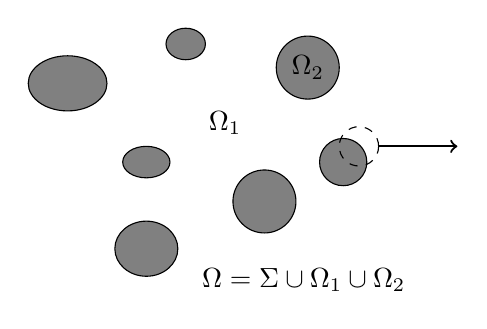
\begin{tikzpicture}
        \foreach \x/\y/\ra/\r in {
        1/3/0.2/0.25,
        2.55/2.7/0.4/0.4,
        0.5/0.4/0.35/0.4,
        2/1/0.4/0.4,
        3/1.5/0.3/0.3,
        0.5/1.5/0.2/0.3,
        -0.5/2.5/0.35/0.5}{
            \draw[fill=gray](\x,\y) ellipse(\r cm and \ra cm);
        }
        \draw[dashed](3.2,1.7)circle(0.25);
        % \draw[thick,->](3.2,1.7)++(0.1767,0.1767)--++(0.4,0.4)--++(1,0);
        \draw[thick,->](3.2,1.7)++(0.25,0)--++(1,0);
        \draw(2.55,2.7)node{$\Omega_2$};
        \draw(1.5,2)node{$\Omega_1$};
        \draw(2.5,0)node{$\Omega = \Sigma \cup \Omega_1 \cup \Omega_2$};
        % \draw(2.5,-1)node{$\Sigma = \sum_\alpha \Sigma_\alpha$};
        % \draw(2.5,-0.5)node{$\Omega_2 = \sum_\alpha \Omega_\alpha$};
    \end{tikzpicture}
    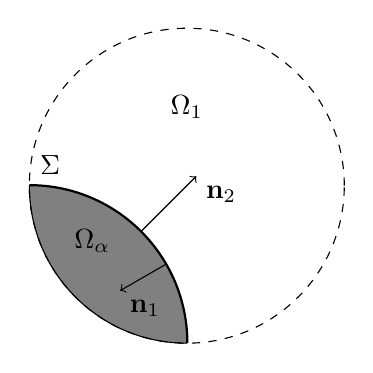
\begin{tikzpicture}%[scale = 0.9]
        \draw[very thick](0:2)arc(0:90:2)node[above right]{$\Sigma$};
        \draw[fill=gray](0:2)arc(0:90:2)arc(180:270:2);
        \draw[dashed](2,2)circle(2);
        \draw[->](1.42,1.42)--++(0.7,0.7)node[below right]{$\textbf{n}_2$};
        \draw[->](1.73,1)--++(-0.577,-0.333)node[below right]{$\textbf{n}_1$};
        \draw(2,3)node{$\Omega_1$};
        \draw(0.8,1.3)node{$\Omega_\alpha$};
    \end{tikzpicture}
    \caption{Scheme of the topology of dispersed two phase flows.}
    \label{fig:Scheme}
\end{figure}
From now on the $k$ indies will refer to either the phase $1$ or $2$, and we drop the time and position arguments in each functions. 
Then, the transport equation of $\chi_k$ can be written as \citep{drew1983mathematical,kataoka1986local,morel2015mathematical},
\begin{equation}
    \pddt \chi_k
    + \textbf{u}_I \cdot \nablabh \chi_k
    = 0,
    \label{eq:dt_chi_k}
\end{equation}
where $\textbf{u}_I$ is the velocity of $\Sigma(t)$.
Besides, it can be shown \citep{tryggvason2011direct,drew1983mathematical,kataoka1986local,bothe2022sharp} that,
\begin{equation}
    \nablabh \chi_k
    = - \delta_I \textbf{n}_k
    \label{eq:grad_chi_k}
\end{equation}
where we have introduced the Interface Indicator Function (IIF) defined as $\delta(\textbf{y}-\textbf{y}_I)$, with $\delta$ being the Dirac-delta function and $\textbf{y}_I$ the position vectors lying on the domain $\Sigma(t)$.
We also define $\textbf{n}_k$ as the outward normal vector of the domain $\Omega_k$.
Taking the gradient of \ref{eq:dt_chi_k} yields the IIF transport equation namely,
\begin{equation}
    \pddt \delta_I
    + \nablabh \cdot \left[(\textbf{u}_I\cdot\textbf{n})\textbf{n} \delta_I\right]
    = \delta_I (\textbf{u}_I\cdot\textbf{n})(\nablabh \cdot\textbf{n})
\end{equation}
As pointed out by \citet{morel2007surface}, it is more convenient to rewrite this equation under the following form,
\begin{equation}
    \pddt \delta_I
    + \nablabh \cdot (\delta_I \textbf{u}_I)
    = \delta_I \nablabhI \cdot \textbf{u}_I.
    \label{eq:dt_delta_I}
\end{equation}
where we introduced the surface divergence operator defined as $\nablabhI \cdot ()= (\textbf{I}-\textbf{nn})\cdot \nablabh \cdot ()$.
Likewise, we can derive an expression for the gradient of $\delta_I$ by taking the gradient of \ref{eq:grad_delta_I} yielding,
\begin{equation}
    % &
    \nablabh\delta_I 
    = \textbf{n} \cdot \nablabh (\textbf{n} \delta_I),
    % &
    % \pddt\delta_I 
    % = - \textbf{n} \cdot \nablabh (\textbf{u}_I  \cdot \textbf{n} \delta_I)
    \label{eq:grad_delta_I}
\end{equation}


Let $f_k(\textbf{y})$ being a volumetric property of the flow solely defined in $\Omega_k(t)$.
Likewise, let $f_I(\textbf{y})$ be an arbitrary surface property defined on $\Sigma(t)$.
Then it is possible to derive the local conservation equations for volumetric and surface quantities \citep{bothe2022sharp,morel2015mathematical,tignol1986modelisation}, using Reynolds transport theorem  and divergence theorem on an arbitrary control volume.
These conservation laws read as, 
\begin{align}
    \label{eq:dt_f_k}
    \pddt f_k
    &= \nablabh \cdot \left(
        \bm{\Phi}_k
        - f_k\textbf{u}_k
        \right)
    + \textbf{S}_k
    & \text{ in } \Omega_k,&\\
    \pddt f_I  
    &= 
    \nablabhI \cdot (\mathbf{\Phi}_{I||} - f_I \textbf{u}_I)
    + \textbf{S}_I
    - \Jump{
        f_k (\textbf{u}_I - \textbf{u}_k)
        + \mathbf{\Phi}_k
     } 
    & \text{ on } \Sigma&
    \label{eq:dt_f_I}
\end{align}
for respectively the volumetric and surface properties.
In \ref{eq:dt_f_I} we introduced the notation $\Jump{\ldots}$ to indicate the sum over both phases, i.e. $\sum_{k=1}^2 [\ldots] \cdot \textbf{n}_k$. 
Where we introduced $\bm{\Phi}_k$ and $\bm{\Phi}_I$ as the non-conservative flux tensor corresponding to $f_k$ and $f_I$. 
The non-conservative flux is often expressed through a constitutive equation depending on the nature of the flow such as the stress tensor for the momentum.
$\textbf{S}_k$ and $\textbf{S}_I$ is defined as the volumetric source term of respectively the phase $k$ and at the interface $\Sigma$.
It is important to notice that \ref{eq:dt_f_k} and \ref{eq:dt_f_I} are solely defined in respectively $\Omega_k$ and $\Sigma$, therefore these equations are referred as local conservation equations.

To generalize these equations over the domain $\Omega$ we follow the formalism of \citet{drew1983mathematical,marle1982macroscopic} and \citet{kataoka1986local} for the volumetric quantities.
Indeed, to any local quantities $f_k$ defined in $\Omega_k$, we assign the field $\chi_k f_k$ which is defined in $\Omega$. 
Similarly, for any local surface quantities $f_I$ defined on $\Sigma$ we assign the field quantity $\delta_I f_I$ defined on $\Omega$. 
Then, multiplying \ref{eq:dt_f_k} and \ref{eq:dt_f_I} by respectively $\chi_k$ and $\delta_I$, and making use of \ref{eq:dt_chi_k} and \ref{eq:dt_delta_I} gives, 
\begin{align}
    \pddt (\chi_k f_k)
    &= \nablabh \cdot (\chi_k \bm{\Phi}_k - \chi_k f_k \textbf{u}_k)
    + \chi_k \textbf{S}_k
    + \delta_I\left[
        \bm{\Phi}_k
        + f_k
        \left(
            \textbf{u}_I
            - \textbf{u}_k
        \right)
    \right]
    \cdot \textbf{n}_k ,
    % & \forall \textbf{y} \in \Omega&
    \label{eq:dt_chi_k_f_k}\\
    \pddt (\delta_If_I)  
    &= 
    \nablabh \cdot (\delta_I \mathbf{\Phi}_{I||} - \delta_I f_I \textbf{u}_I)
    +\delta_I\textbf{S}_I 
    - \delta_I \Jump{
    f_k (\textbf{u}_I - \textbf{u}_k)
    + \mathbf{\Phi}_k
    }.
    \label{eq:dt_delta_I_f_I}
\end{align}
We obtained $k$'s equations defined over the domain $\Omega$ for the bulk quantities, and third global equations for the surface quantities also valid over $\Omega$. 
The transformation of these equations from local to global conservation makes appear a term on the RHS of \ref{eq:dt_chi_k_f_k} representing the interfacial transfer of $f_k$ and $\mathbf{\Phi}_k$, while the surface transport equation did not change fundamentally. 
The set of equations formed by \ref{eq:dt_chi_k_f_k} for $k =1,2$ is commonly known as the \textit{two-fluid} formulation of multiphase flows, to which we add the \textit{jump condition} across the phase given by \ref{eq:dt_delta_I_f_I} \citep{morel2015mathematical,tryggvason2011direct,drew1983mathematical,kataoka1986local}. 
In this work, we prefer to think of those equations as a set of three equations, formed by \ref{eq:dt_chi_k_f_k} for the volumetric conservation equations and \ref{eq:dt_delta_I_f_I} for the surface conservation equations. 

Now that we properly defined the volumetric and surface conservation laws over $\Omega$, let's derive of two phase flows.
We now define any bulk quantity $f$ as $f = \sum_k \chi_k f_k + \delta_I f_I$.
Then adding \ref{eq:dt_chi_k_f_k} for $k=1,2$ and \ref{eq:dt_delta_I_f_I} give the commonly known as the \textit{single-fluid} formulation,
\begin{equation}
    \pddt f
    = \nablabh \cdot (\bm{\Phi} - f \textbf{u})
    + \textbf{S}.
    \label{eq:dt_f}
\end{equation}
Actually, it is more common in the literature to define the bulk quantities as $f = \sum_k \chi_k f_k$ and consider the interfacial terms as source terms as it is often neglected \citep{morel2015mathematical,tryggvason2011direct}. 
Nevertheless, in this work we consider a general case without approximation therefore it is more convenient to think of the bulk quantities as a sum of three phase quantities. 

\subsection{The averaged conservation equations}
\label{sec:avg_def}
In this study, we employ the ensemble average technique to establish the averaged conservation equations. 
This method is just one of several averaging approaches, including the volume average method \citep{jackson1997locally} and time averaging \citep{ishii2010thermo}. 
Despite their differences, all these techniques yield the same set of averaged equations \citep{jackson1997locally,zhang1997momentum}.
In the following we recall some properties of the ensemble average operator. 
Let, $P(\FF)$ be the probability density function that describes the probability of finding the flow in the configuration $\FF$. 
We note $d\PP = P(\FF) d\FF$ the probable number of flows located in the incremental region of the phase space $d\FF$ around the point $\FF$. 
It follows from this definition, that the ensemble average of an arbitrary local property $f^0(\textbf{x},t;\FF)$ defined on the whole space $\Omega$, is,
\begin{equation}
    f(\textbf{x},t)
    = \avg{f^0}(\textbf{x},t)
    =\int f^0(\textbf{x},t;\FF) d\mathscr{P}. 
    \label{eq:avg}
\end{equation}  
Note that we dropped the super script $^0$ on $f(\textbf{x},t)$ to indicate that this is an averaged quantity. 
The macroscopic variables are averaged over all $\FF$, and therefore depend only on $\textbf{x}$ and $t$.
Thus, we omit the arguments of the averaged fields, as this notation eliminates any potential ambiguity. 
The ensemble average quantities are assumed to satisfy the following properties \citep{drew1983mathematical}
\begin{align}
    \label{eq:avg_properties}
    \avg{f^0+h^0} &= f+h, \\ 
    \avg{\avg{f^0}h^0} &= fh, \\
    \avg{\pddt f^0} 
    &= \pddt f, \\ 
    \avg{\grad f^0}
    &= \grad f. 
\end{align}
were $f$ and $h$ are two arbitrary Eulerian fields. 
The first two relations are called the Reynolds' rules, the third one is the Leibniz' rule and the last one, is the Gauss' rule \citep{drew1983mathematical}.
Additionally, for any phase quantity defined in $\Omega_k$ we introduce the definition, 
\begin{equation}
    \phi_k f_k (\textbf{x},t) = \avg{\chi_k f_k^0},
    \label{eq:1_avg}
\end{equation}
where $\phi_k(\textbf{x},t) = \avg{\chi_k}$ is the volume fraction of the phase $k$.
And $f_k$ is the average of the field $f_k^0$ conditioned on the presence of the phase $k$ in the configuration $\FF$ at $\textbf{x}$ and time $t$.
Equally, for interface quantities we have 
\begin{equation}
    \phi_I f_I (\textbf{x},t) = \avg{\delta_I f_I^0},
\end{equation}
with $\phi_I = \avg{\delta_I}$ the interfacial area concentration function. 
Here, $f_I$ is the average of $f^0_I$ conditioned on the presence of an interface in the configuration $\FF$ at $\textbf{x}$ and time $t$. 
Additionally, we define the field of fluctuation of a given quantity around its mean as,
\begin{align}
    f'(\textbf{x},t,\FF) = f^0(\textbf{x},t,\FF) - f(\textbf{x},t).
    \label{eq:def_fluctu}
\end{align}
This relation applies to phase averaged quantities such that $f'_k = f^0_k - f_k$ and $f'_I = f^0_I - f_I$. 


Applying the ensemble average on \ref{eq:dt_chi_k_f_k} and \ref{eq:dt_delta_I_f_I} and considering the properties from \ref{eq:avg_properties} to \ref{eq:def_fluctu}, yields the general form of the averaged equations of multiphase flows, namely,
\begin{align}
    \pddt (\phi_k f_k)
    +\div (\phi_k f_k \textbf{u}_k - \mathbf{\Phi}_k^\text{eq})
    &= 
    \phi_k s_k
    + \avg{\delta_I\left[
        \mathbf{\Phi}_k^0
        + f_k^0
        \left(
            \textbf{u}_I^0
            - \textbf{u}_k^0
        \right)
    \right]
    \cdot \textbf{n}_k} ,
    \label{eq:avg_dt_chi_f}\\
    \pddt (\phi_I f_I)
    +\div (\phi_I f_I \textbf{u}_I- \mathbf{\Phi}_{I}^\text{eq})
    &= 
    \phi_I s_I
    - \avg{\delta_I 
    \Jump{
    f_k^0 (\textbf{u}_I^0 - \textbf{u}_k^0)
    + \mathbf{\Phi}_k^0
    } 
     },
    \label{eq:avg_dt_delta_f}
\end{align}
with, 
\begin{align*}
    \mathbf{\Phi}_k^\text{eq}
    = \avg{\chi_k f_k' \textbf{u}_k'}
    - \phi_k \bm\Phi_k,
    &&
    \mathbf{\Phi}_{I}^\text{eq}
    = \avg{\delta_I f_I' \textbf{u}_I'}
    - \phi_I \bm\Phi_I. 
\end{align*}
These equations are to be solved for the averaged field $\phi_k,\phi_I,f_k$ and $f_I$ with a complementary equation of volume conservation, i.e. $\phi_f+\phi_d+\phi_I = 1$.
The main differences between these equations and their microscale counterparts (\ref{eq:dt_f_k} and \ref{eq:dt_f_I}) are:
(1) The unknowns are now averaged quantities,
(2) Factors $\phi_k$ and $\phi_I$ are introduced in front of all the terms, and
(3) The additional terms $\avg{\chi_k f_k' \textbf{u}_k'}$ and $\avg{\delta_I f_I' \textbf{u}_I'}$ appear, representing the covariance between the conserved quantity ($f_k$ or $f_I$) and the local velocities.  
For a complete understanding, we derived the mass, momentum, and energy averaged equations in \ref{ap:two-fluid_model}. 
These are derived considering the simplifying hypothesis exposed in \ref{ap:hypothesis}. 
In addition, \ref{ap:two-fluid_model} presents how to derive the secondary averaged equations of the averaged energy $E_k$, i.e. the equation for the mean internal energy $e_k$, the pseudo turbulent energy $k_k = \frac{1}{2\phi_k}\avg{\chi_k (u'_k)^2}$, and the averaged kinetic energy $(u_k)^2/2$.  


It is important to highlight that the two-fluid model fails to adequately distinguish between the two phases, as evidenced by the \textit{symmetry} $k = 1$ and $2$ in the aforementioned equations. This symmetry does not hold physically because the dispersed phase possesses a distinct topological nature compared to the continuous phase. 
More importantly, in a dispersed two-phase flow system the closure terms are expressed as a function of the Lagrangian properties of the particles whereas this system of equation provides us with continuously averaged quantities. 
Specifically, the mean drag force or torque term in the averaged momentum equation is expressed as a function of the center of mass linear and angular velocity  of the particles. 
Whereas this system of equation provides us with the phase averaged velocity of the whole phase not with no consideration for the particles properties.  
Therefore, in the subsequent section, we will introduce a kinetic model specifically devoted to the dispersed phase. 
As illustrated below, the equations governing the dispersed phase are more comprehensive as they bear a resemblance to the equations governing a single particle.



\section{Lagrangian equations for the dispersed phase}
\label{sec:Lagrangian}

In this section, we present a Lagrangian-based model capable of describing the dispersed phase with an arbitrary order of accuracy.

\subsection{Fundamental properties}

At this stage, we define some fundamental properties associated to each particle labeled $\alpha$.
Following the strategy of \citet{lhuillier2009rheology,lhuillier1992volume,zaepffel2011modelisation} and \citet[Chapter 2]{morel2015mathematical}
we define the mass $m_\alpha$, position of center of mass $\mathbf{x}_\alpha$, and the momentum $\textbf{p}_\alpha$ of the particle $\alpha$, as
\begin{align}
    m_\alpha(t,\FF)
    = \intO{ \rho_d  }, 
    &&
    \textbf{x}_\alpha(t,\FF)
    = \frac{1}{m_\alpha(t,\FF) }\intO{ \rho_d \textbf{x} }, 
    &&\textbf{p}_\alpha(t,\FF) 
    = \intO{ \rho_d \textbf{u}_d^0 }.
    \label{eq:mass_pos}
    % \label{eq:momentum_energy}
\end{align}
$\Omega_\alpha(t,\FF)$ is the time-dependent domain occupied by the particle $\alpha$ (see \ref{fig:Scheme}). 
Subsequently, we define the velocity of the particle center of mass as
\begin{equation*}
\textbf{u}_\alpha = \frac{d \textbf{x}_\alpha}{dt}.
\end{equation*}
Replacing $\textbf{x}_\alpha$ by its definition (\ref{eq:mass_pos}) we obtain
\begin{equation*}
    \textbf{u}_\alpha = \frac{1}{m_\alpha}
    \frac{d}{dt} 
    \left(
        \intO{ \rho_d \textbf{x} }
    \right)
    - \frac{1}{m_\alpha^2} \frac{d}{dt} \left(\intO{ \rho_d } \right)
    \intO{ \rho_d \textbf{x} }.
\end{equation*}
%\tb{ A finaliser
Using the Reynolds transport theorem (\ref{eq:reynolds_transport}) for both terms in parentheses and making use of the conservation of mass (\ref{eq:dt_rho}) and the definition of $\textbf{x}_\alpha(t,\FF)$ in the last term, gives
\begin{equation}
    \textbf{u}_\alpha = 
    \frac{1}{m_\alpha}\intO{ \left[
        \pddt (\textbf{x}\rho_d ) + \div\left(\textbf{u}_d \textbf{x} \rho_d\right) 
    \right]} \\
    + \frac{1}{m_\alpha}\intS{ \textbf{x} \rho_d(\textbf{u}_I   - \textbf{u}_d) \cdot \textbf{n}_d }
    -  \frac{\textbf{x}_\alpha}{m_\alpha}    \intS{ \rho_d(\textbf{u}_I   - \textbf{u}_d) \cdot \textbf{n}_d }
\end{equation}
Then by considering the mass conservation for the first term and noticing that $\grad \textbf{x} = \bm\delta$, for the second term gives, 
\begin{equation}
    \textbf{u}_\alpha(t,\FF) = \frac{1}{m_\alpha(t,\FF)} \left(
        \textbf{p}_\alpha(t,\FF)
        +  \intS{\rho_d \textbf{r} (\textbf{u}_I^0 - \textbf{u}_d^0)\cdot \textbf{n}_d }
        \right),
        \label{eq:dt_y_alpha}
\end{equation}
where $\textbf{r}(\textbf{x},t) = \textbf{x} - \textbf{x}_\alpha(t)$. 
In \ref{eq:dt_y_alpha}, it can be observed that the first component of the velocity represents the linear momentum divided by the mass of the particle. 
This corresponds to the mass-averaged velocity over the volume of the particle.
The second term in \ref{eq:dt_y_alpha} arises from the contribution of anisotropic mass transfer across the surface of the particle. 
This mass transfer leads to the motion of the particle's center of mass, thereby contributing to the total velocity.
To illustrate this concept, let us consider a fixed drop with no momentum lying over a very hot plate.
In this scenario, we assume that the plate is sufficiently hot to induce evaporation, specifically on the bottom portion of the drop.
Hence, under the effect of an anisotropic evaporation flux one may expect the second term to be non-negligible.
Consequently, the center of mass of the drop has a non-zero velocity in the opposite direction of the plate, even though the momentum is assumed to be zero.
Note that \ref{eq:dt_y_alpha} generalized usual expression of the center of mass velocity whom neglect the second term.
In the following, for the sake of brevity we discard the dependency on $t$ and $\FF$ on the notations for all Lagrangian quantities denoted by the subscript $_\alpha$ and in particular $\Gamma_\alpha$ and $\Omega_\alpha$.
Nevertheless, the reader must understand that all Lagrangian quantities and integration domains subscribed by $_\alpha$ are time and configuration-dependent. 

The particle's internal relative motions or the \textit{inner velocity} is given by $\textbf{w}_d^0 = \textbf{u}_d^0 - \textbf{u}_\alpha$. 
Substituting the inner velocity in the momentum definition (\ref{eq:mass_pos}) yields
\begin{equation}
    \label{eq:momentum_definition_1}
    \textbf{p}_\alpha
    = m_\alpha \textbf{u}_\alpha
    + \int_{\Omega_\alpha} \rho_d \textbf{w}_d^0 d\Omega.
\end{equation}
Alternatively, from \eqref{eq:dt_y_alpha}, we obtain,
\begin{equation}
    \textbf{p}_\alpha
    =  m_\alpha \textbf{u}_\alpha
    - \int_{\Gamma_\alpha} \rho_d\textbf{r}(\textbf{u}_I^0 - \textbf{u}_d^0)\cdot \textbf{n}_d d\Sigma
    \label{eq:momentum_definition}
\end{equation}
Therefore, the momentum of a particle can be seen as a sum of the mean velocity plus the integral of the fluctuation (\ref{eq:momentum_definition_1}), with the latter being equivalent to minus the first moment of mass transfer term (\ref{eq:momentum_definition}).
Indeed, by identification we obtain : $\intO{ \rho_d \textbf{w}_d^0 } = - \intS{  \rho_d\textbf{r} (\textbf{u}_I^0 - \textbf{u}_d^0)\cdot \textbf{n}_d }$. 
Hence, the internal velocity fluctuations within a fluid particle do not contribute to the total linear momentum $\textbf{p}_\alpha$, as long as the anisotropic mass transfer is negligible.  
Only within this simplified context we can consider the classic relation $\textbf{p}_\alpha = m_\alpha \textbf{u}_\alpha$. 

\subsection{Conservation laws}

We assign to a particle indexed, $\alpha$, occupying the domain $\Omega_\alpha$ (see \ref{fig:Scheme}) an arbitrary Lagrangian property $q_\alpha$ defined by $q_\alpha  = \intO{ f_d^0}$.
Similarly, we define $q_{I\alpha} = \intS{ f_I^0}$ as an integrated surface property of the particle $\alpha$.

\subsubsection{Inside the volume}
To describe the evolution of any arbitrary Lagrangian quantity $q_\alpha$, we need to establish its time derivative.
Since $q_\alpha$ is an integral quantity with a time-dependent domain of integration, we apply the general Reynolds transport theorem for volume integral which gives for material domains (here the droplet volume),
\begin{equation}
    \ddt  \intO{f_d^0}
    = \intO{\left[ \pddt f_d^0 + \div\left(f_d^0\textbf{u}_d^0\right) \right]}\\
    + \intS{ f_d^0 (\textbf{u}_I^0-\textbf{u}_d^0)\cdot \textbf{n}_d }.
    \label{eq:reynolds_transport}
\end{equation}
By substituting the integrand of the first integral on the right-hand side (RHS) with \ref{eq:dt_f_k} we obtain the conservation law of the quantity $q_\alpha$, namely,  
\begin{equation}
    \ddt{q_\alpha}
    = \intO{ s_d^0 }
    + \intS{ \left[
        f_d^0 (\textbf{u}_I^0-\textbf{u}_d^0) 
        + \mathbf{\Phi}_d^0 
        \right] \cdot \textbf{n}_d }.
    \label{eq:dt_q_alpha}
\end{equation}
In \ref{eq:dt_q_alpha} we used the Gauss divergence theorem to show that
\begin{equation}
    \intO{\div \mathbf{\Phi}_d^0} = \intS{\mathbf{\Phi}_d^0 \cdot \textbf{n}_d}.
\end{equation}
The first term on the right-hand side of \ref{eq:dt_q_alpha} accounts for the total contribution of the source term $s_d^0$ to the particle $\alpha$,
while the second term is the surface integration of the exchange terms, which includes the phase transfer flux $f_d^0 (\textbf{u}_I^0-\textbf{u}_d^0)$ and the diffusive flux $\mathbf{\Phi}_d^0$. 


Let us consider the specific case of the momentum balance, i.e. $q_\alpha = \textbf{p}_\alpha$.
In this situation, \ref{eq:dt_q_alpha} reads
\begin{equation}
    \ddt  \textbf{p}_\alpha
    = \intO{ \rho_d\textbf{g} }
    + \intS{ 
        \left[
        f_d^0 (\textbf{u}_I^0-\textbf{u}_d^0)
         + \bm{\sigma}_d^0%\cdot\textbf{n}_d  
        %+ \mathbf{\Phi}_d^0 
        \right] 
        \cdot \textbf{n}_d },
\end{equation}
% first term reads as $\intO{ \rho_d\textbf{g} }$ 
The first term on the right-hand side represents the total weight acting on the particle $\alpha$, 
the second term represents the total source of momentum due to phase transfer, and it is expressed as, $\intS{ \rho_d \textbf{u}_d^0 (\textbf{u}_I^0-\textbf{u}_d^0)\cdot\textbf{n}_d }$,
and the last term $\intS{ \bm{\sigma}_d^0\cdot\textbf{n}_d }$, represents the resultant of the hydrodynamic forces acting on the surface of the particle.
It is important to notice that under this form, the exchange terms are expressed as integrals of dispersed phase fields denoted by the subscript $_d$.
Nevertheless, depending on the nature of the dispersed phase, these fields may not always be defined.
For rigid particles the stress within the particle $\bm{\sigma}_d^0$ is indeterminate \citep{guazzelli2011}.  
Hence, our objective is to express these exchange terms, in terms of the continuous phase field quantities instead of the dispersed phase fields, i.e. in terms of $\mathbf{\Phi}_f^0$ and $\textbf{u}_f^0$ rather than $\mathbf{\Phi}_d^0$ and $\textbf{u}_d^0$. 

\subsubsection{On the interfaces}
To address this issue in a general manner, let us derive the conservation equation for the integrated surface property $q_{I\alpha} = \intS{f_I^0}$.
To differentiate time-varying surface integrals within time, we make use of the general Leibniz rule, which states that for an arbitrary function $f_I^0$ defined on $\Gamma(t)$ we have the relation \citep{nadim1996concise}
\begin{equation}
    \ddt  \intS{f_I^0 }
    = \intS{ \left[
        \pddt f_I^0
        +   \gradI \cdot (\textbf{u}_I^0f_I^0)
    \right]}.
    \label{eq:surface_derivative}
\end{equation}
Substituting the right-hand side terms of \ref{eq:surface_derivative} with \ref{eq:dt_f_I}, gives,
\begin{equation}
    \ddt  q_{I\alpha}
    = \intS{ 
        s_I^0
    }
    - \intS{
 \Jump{
        f_k^0 (\textbf{u}_I^0 - \textbf{u}_k^0)
        + \mathbf{\Phi}_k^0
    }
    }.
    \label{eq:dt_q_I_alpha}
\end{equation}
We have used the surface divergence theorem applied to closed surfaces \citep{nadim1996concise}, it reads
\begin{equation}
    \intS{\gradI F}
    = 
    \intS{ F \textbf{n} (\div \textbf{n})},
    \label{eq:gauss_surface}
\end{equation} 
where $F$ is an arbitrary field.
This theorem demonstrates that any surface property parallel to the tangential plane of $\Gamma$, such as $\bm\Phi_{I||}$, satisfies the relation $\intS{\divI \bm\Phi_{I||}^0}
= 0$.
This explains why $\bm\Phi_{I||}$ does not appear in \ref{eq:dt_q_I_alpha}. 
\ref{eq:surface_derivative} can be interpreted as the conservation equation for the integrated surface property $f_I^0$, or as the jump condition of the $f^0_k$ integrated on the droplet surface. 
As discussed above we wish to get rid of $\mathbf{\Phi}_d^0$ in \ref{eq:dt_q_alpha}. 
To achieve this, we treat the particle's volume and surface as a unified entity and derive a conservation equation for $q_\alpha^\text{tot} = q_\alpha + q_{I\alpha}$. 
By summing \ref{eq:dt_q_alpha} and \ref{eq:dt_q_I_alpha} we directly obtain 
\begin{equation}
    \ddt  q_\alpha^\text{tot}
    = 
    \intO{ s_d^0 }
    + \intS{ s_I^0 }
    + \intS{ \left[
        f_f^0 (\textbf{u}_I^0-\textbf{u}_f^0) 
        + \mathbf{\Phi}_f^0 
        \right] \cdot \textbf{n}_d }. 
    \label{eq:dt_q_alpha_tot}
\end{equation}
This equation is the general form of the linear conservation law for the quantity $q_\alpha^\text{tot}$.
It applies to any particle immersed into a continuous phase following the local conservation, \ref{eq:dt_f_k} and \ref{eq:dt_f_I}.
We refer to this equation as the zeroth-order conservation equation or the linear conservation law for the particle $\alpha$.

We would like to highlight that due to the consideration of closed surface, the diffusive flux $\mathbf{\Phi}_{I||}^0$, plays no role at all in \ref{eq:dt_q_alpha_tot}.
Therefore, in the case of the linear momentum conservation law, the contribution of the momentum diffusive flux $\bm\sigma_{I||}^0$ exposed in \ref{eq:dt_rhoIu_I}, will not contribute to the momentum balance of a particle, and we obtain the relation 
\begin{equation}
    \ddt  \textbf{p}_\alpha^\text{tot}
    = 
    \intO{ \rho_d^0\textbf{g} }
    + \intS{ \rho_I^0\textbf{g} }
    + \intS{ 
        \left[
        f_d^0 (\textbf{u}_I^0-\textbf{u}_f^0)
        + \bm{\sigma}_f^0
        \right] 
        \cdot \textbf{n}_d }. 
\end{equation}
In this case, note that $\textbf{p}_\alpha^\text{tot} = \intO{\rho^0_d \textbf{u}_d^0}+\intS{\rho^0_I \textbf{u}_I^0}$ is the momentum of the particle's volume and surface. 
The latter might be negligible if the interface has a negligible weight. 
As a consequence, even in the presence of local Marangoni forces or surface viscous stresses (see \ref{eq:surface_fluxes}), the resultant of the surface diffusive fluxes would still cancel out in the linear momentum balance.
This fact has already been demonstrated by \citet{hesla1993note} who showed that the surface tension force does not contribute to the linear and angular momentum balance. 
Here, we have provided the general proof that the interfacial diffusive flux $\mathbf{\Phi}_{I||}^0$, which is present at the local scale according to \ref{eq:dt_f_I}, does not contribute to the zeroth-order conservation law of a particle with a closed surface.

For completeness, we exposed in \ref{ap:particles_eq} a clear derivation of the mass, momentum and total energy equations for a single particle.
The derivation takes place using the same hypothesis as it is exposed in \ref{ap:hypothesis}.
Especially, it is shown that the integration of the kinetic energy jump condition corresponds to the Lagrangian derivative of the particle surface, see \ref{eq:int_u_I2}. 

\subsection{Higher moment equations}

Because $f_d^0$ and $f_I^0$ are not always constant over the volumes and surfaces of the particles, it is interesting to introduce in the first place, the first moment of the quantities $f_d^0$ and $f_I^0$. 
They are defined as
\begin{align}
    &\textbf{Q}_\alpha 
    = \intO{ \textbf{r} f_d^0 },
    &\text{and}&
    &\textbf{Q}_{I\alpha}
    = \intS{ \textbf{r} f_I^0 },
    \label{eq:first_moment_definition}
\end{align}
where we recall that $\textbf{r} = \textbf{x} - \textbf{x}_\alpha$ is the distance between any point inside $\Omega_\alpha$ or $\Gamma_\alpha$, to the center of mass of the particle $\alpha$.
It is then possible to differentiate these moments with respect to time to obtain their conservation laws.
We use the Reynolds transport theorem (\ref{eq:reynolds_transport}) to describe the evolution of $\textbf{Q}_\alpha$ within time. 
It gives, 
\begin{equation*}
    \frac{d}{dt} \textbf{Q}_\alpha
      =  \intO{\left[
        \pddt(  f_d^0\textbf{r})
        + \div \left(  f_d^0 \textbf{r}\textbf{u}_d^0\right)
    \right]} 
    + \intS{  f_d^0 \textbf{r}  (\textbf{u}_I^0-\textbf{u}_d^0)\cdot \textbf{n}_d}
\end{equation*}
The first term on the right-hand side may be rewritten as
\begin{equation*}
\intO{ \left[
        \pddt(\textbf{r}  f_d^0)+ \div \left( \textbf{u}_d^0 \textbf{r} f^0_d\right) 
    \right]}
    = \intO{\textbf{r}\left[
        \pddt f_d^0
        + \div \left(f_d^0 \textbf{u}_d^0\right)
    \right] }
    + \intO{ f_d^0 \left[
        \pddt \textbf{r}
        +(\textbf{u}_d^0 \cdot \grad) \textbf{r}
    \right]}
\end{equation*}
Using \ref{eq:dt_f_k} for the first integral on the right-hand side, and considering the relation,
$  \pddt \textbf{r}
+ (\textbf{u}_d^0 \cdot \grad) \textbf{r}
= - \frac{d}{dt} \textbf{y}_\alpha  + \textbf{u}_d^0 
= \textbf{w}_d^0$,
for the second integral yields 
\begin{align}
    \frac{d}{dt} \textbf{Q}_\alpha
    % &= \intO{\textbf{r} \left[
    %      s_d^0  +  \div \bm\Phi_d^0
    % \right]}
    % +\intO{f_d^0  \textbf{w}_d }
    % + \int_{\Gamma_\alpha} \textbf{r}  f_d^0 (\textbf{u}_I^0-\textbf{u}_d^0)\cdot \textbf{n}_d  d\Sigma,\\
    = \intO{\left( 
        \textbf{r} s_d^0  
        + f_d^0  \textbf{w}_d 
        - \bm\Phi_d^0
    \right) }
    + \int_{\Gamma_\alpha} \textbf{r} \left[
        \bm\Phi_d^0
        + f_d^0 (\textbf{u}_I^0-\textbf{u}_d^0)
    \right]\cdot \textbf{n}_d  d\Sigma.
    \label{eq:dt_Q_alpha}
\end{align}
Where we have used the relation $\intO{\textbf{r}  \div \bm\Phi_d^0 }
= \intS{ \textbf{r} \bm\Phi_d^0 \cdot \textbf{n}_d }
- \intO{ \bm\Phi_d^0 }$. 
\ref{eq:dt_Q_alpha} is the first order moment conservation equation for the particle $\alpha$. 
Following the same procedure, and making use of \ref{eq:surface_derivative}, \ref{eq:gauss_surface} and \ref{eq:dt_f_I}, one can equally show that 
\begin{align}
    \ddt {\textbf{Q}_{I\alpha}}
    &= \intS{ \left(
        \textbf{r}s_I^0
        + f_I^0 \textbf{w}_I^0
        - \mathbf{\Phi}_{I||}^0
    \right) }
    - \intS{\textbf{r} 
    \Jump{\mathbf{\Phi}_k^0
        + f_k^0 (\textbf{u}_I^0 - \textbf{u}_k^0)
    }
    },
    \label{eq:dt_Q_I_alpha}
\end{align}
where $\textbf{w}_I^0 = \textbf{u}_{I||}^0 - \textbf{u}_\alpha$.
In \ref{eq:dt_Q_alpha}, we recognize the first moment of the source term $s_d^0$, the first moment of the diffusive flux term $\bm\Phi_d^0\cdot\textbf{n}_d$ and the first moment of phase exchange term, $f_d^0 (\textbf{u}_I^0-\textbf{u}_d^0)\cdot\textbf{n}_d$. 
Additionally, two supplementary terms appear in \ref{eq:dt_Q_alpha}, namely: the integral of the diffusive flux $\bm\Phi_d^0$, and a term related to the fluctuation of the internal velocity $f_d^0 \textbf{w}_d^0$.
Similar observations can be made for the first moment of surface equation \ref{eq:dt_Q_I_alpha}, as it shares similarities with \ref{eq:dt_Q_alpha}. 
In particular, it is worth noting the presence of the surface diffusive flux $\mathbf{\Phi}_{I||}^0$ in \ref{eq:dt_Q_I_alpha}.
This term will be further discussed in the following. 

For similar reason than the linear conservation equations, we sum \ref{eq:dt_Q_alpha} and \ref{eq:dt_Q_I_alpha} to expresses the conservation equation of the total first moment $\textbf{Q}_\alpha^\text{tot} = \textbf{Q}_\alpha + \textbf{Q}_{I\alpha}$, this yields 
\begin{multline}
    \ddt {\textbf{Q}_\alpha^\text{tot}}
    = \intO{ \left(
        \textbf{r} s_d^0         
        + f_d^0  \textbf{w}_d^0 
        - \mathbf{\Phi}_d^0
    \right) }
    + \intS{ \left(
        \textbf{r}s_I^0
        + f_I^0 \textbf{w}_I^0
        - \mathbf{\Phi}_{I||}^0
    \right) }
    + \intS{ \textbf{r} \left[
        \mathbf{\Phi}_f^0
        + f_f^0 (\textbf{u}_I^0-\textbf{u}_f^0)
    \right]\cdot \textbf{n}_d  }. 
    \label{eq:dt_Q_alpha_tot}
\end{multline}
Likewise, conservation laws can be derived for the $n^{th}$ order moments of volume and surface, i.e. for
\begin{align}
    \textbf{Q}_{\alpha n}
    = \intO{
         \underbrace{\textbf{rr}\ldots \textbf{rr}}_{n\text{ times}}
        f_d^0 },
        && \text{and} &&
    \textbf{Q}_{I\alpha n}
    = \intS{
         \underbrace{\textbf{rr}\ldots \textbf{rr}}_{n\text{ times}}
    f_I^0 },
    \label{eq:Q_n_definition}
\end{align} 
respectively. 
It can be shown that the derivative with time of $\textbf{Q}_{\alpha n}$ and $\textbf{Q}_{I\alpha n}$ do not involve any additional terms than in \ref{eq:dt_Q_alpha} and \ref{eq:dt_Q_I_alpha}, but rather just the $n^{th}$ order moments of the already presented terms.
We provide the full derivation of $\ddt{ \textbf{Q}_{\alpha n}}$ in \ref{ap:Moments_equations}.
In short, these higher order moments describe the distributions of the local quantities $f_d^0$ and $f_I^0$ inside the domain $\Omega_\alpha$ and $\Gamma_\alpha$, respectively.
Consequently, an infinite number of moments would be theoretically necessary to recover the fields $f_d^0$ and $f_I^0$ within $\Omega_\alpha$ and $\Gamma_\alpha$. 
Thus, one can reach an arbitrary order of accuracy upon the knowledge of an arbitrary number of moments for a given quantity.  

\subsection{Discussion}

To gain physical insight into the meaning of the first and higher moment equations, we now consider the case of mass and momentum conservation laws for a particle of arbitrary shape. 
For ease of understanding, we adopt the simplifying hypotheses presented in \ref{ap:hypothesis}. 
This implies that we consider no mass transfer across phases and no surface properties except for surface tension forces.

Following \ref{eq:Q_n_definition} we define the second-order moment of mass and the first-order moment of momentum as respectively,
\begin{equation}
    \textbf{M}_\alpha 
    = \intO{ \rho_d \textbf{r} \textbf{r} }
    \;\;\;\text{and}\;\;\;
    \textbf{P}_\alpha 
    = \intO{ \rho_d \textbf{r} \textbf{u}_d^0 }.
    \label{eq:first_moment_of_momentum_def}
\end{equation}
Note that $\textbf{M}_\alpha$ is analogous to the inertia tensor $\textbf{I}_\alpha$ in solid mechanics, both are related through the expression $\textbf{I}_\alpha = \bm\delta : \textbf{M}_\alpha - \textbf{M}_\alpha$.
For a constant density, the tensor $\textbf{M}_\alpha$ describes the second moment of the volume distribution around the particle center of mass.
Likewise, the tensor $\textbf{P}_\alpha$ describes the first moment of the velocity distribution within the particle volume. 
To provide a clearer physical interpretation of the moment of momentum tensor, we decompose $\textbf{P}_\alpha$ into two distinct parts. 
Namely, 
$\textbf{P}_\alpha = \textbf{S}_\alpha+\textbf{T}_\alpha$, where $\textbf{S}_\alpha$ represents the symmetric part and $\textbf{T}_\alpha$ is the antisymmetric part of $\textbf{P}_\alpha$.
Then, the tensors $\textbf{S}_\alpha$ and $\textbf{T}_\alpha$ correspond respectively to the stretching and angular momentum of the particle $\alpha$. 
The tensor $\textbf{S}_\alpha$ quantifies how fast and in which direction the particle gets elongated or flattened, in other words it represents the mean rate of deformation experienced by the particle.
The tensor $\textbf{T}_\alpha$ is related to the angular momentum of the particle denoted by the pseudo vector $\bm\mu_\alpha = \intO{ \rho_d \textbf{r} \times \textbf{u}_d^0 }$. 
Indeed, both  $\textbf{T}_\alpha$ and $\bm{\mu}_\alpha$ represent the angular momentum and are related through $(\bm{\mu}_\alpha)_i = \epsilon_{ijk} (\textbf{P}_\alpha)_{jk}= \epsilon_{ijk} (\textbf{T}_\alpha)_{jk}$, where $\bm\epsilon$ is the third order alternating unit tensor or Levi-Cita tensor. 
Lastly, we also introduce the scalar $M_\alpha =\frac{1}{3}\bm\delta : \textbf{P}_\alpha = \frac{1}{3}\intO{ \rho_d \textbf{r} \cdot \textbf{u}_d^0 }.$, which quantifies the rate at which the particle is being compressed or expanded.
To better explain the implication of these quantities on the particle kinematics we provide in \ref{eq:scheme}, three schemes representing possible inner velocity fields with their corresponding value of the moment of momentum tensor.
Note that in \ref{eq:scheme} we explicit
\begin{figure}[h!]
    \centering
    \hfill
    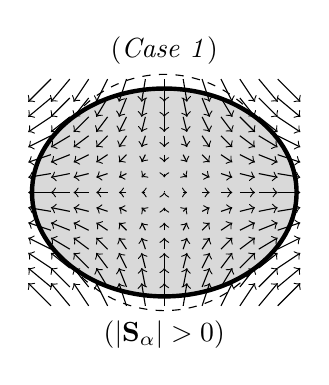
\begin{tikzpicture}[ultra thick,scale=0.6]
        \def\nRows{6}
        \def\nCols{6}
        \draw[dashed,thin] (0,0)circle(2.5);
        \draw[fill=gray!30] (0,0)ellipse(2.8 and 2.2);
        \foreach \x in {-\nRows,...,\nRows} {
            \foreach \y in {-\nCols,...,\nCols} {
                \pgfmathsetmacro\distance{veclen(\x*0.4, \y*0.4)};
                \pgfmathparse{\distance < 2.45 ? "blue" : "white"}
                \edef\colour{\pgfmathresult};
                \ifthenelse{\equal{\colour}{blue}}{                    
                    \draw[thin,->](\x*0.4,\y*0.4)--++(0.08*\x,-0.08*\y);
                }
            }
        }
        \node (txt) at (0,3){(\textit{Case 1})};
        \node (txt) at (0,-3){($|\textbf{S}_\alpha| > 0$)};
    \end{tikzpicture}
     \hfill
    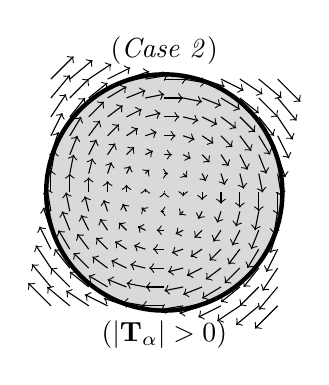
\begin{tikzpicture}[ultra thick,scale=0.6]
        \def\nRows{6}
        \def\nCols{6}
        \draw[fill=gray!30] (0,0)circle(2.5);
        \foreach \x in {-\nRows,...,\nRows} {
            \foreach \y in {-\nCols,...,\nCols} {
                \pgfmathsetmacro\distance{veclen(\x*0.4, \y*0.4)};
                \pgfmathparse{\distance < 2.5 ? "blue" : "white"}
                \edef\colour{\pgfmathresult};
                \ifthenelse{\equal{\colour}{blue}}{                    
                    \draw[thin,->](\x*0.4,\y*0.4)--++(0.08*\y,-0.08*\x);
                }
            }
        }
        \node (txt) at (0,3){(\textit{Case 2})};
        \node (txt) at (0,-3){($|\textbf{T}_\alpha| > 0$)};
    \end{tikzpicture}
    \hfill
    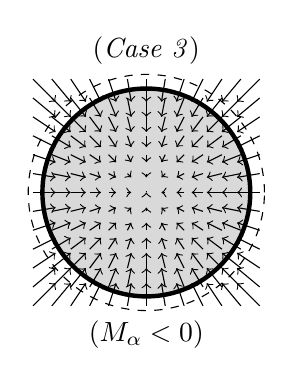
\begin{tikzpicture}[ultra thick,scale=0.6]
        \def\nRows{6}
        \def\nCols{6}
        \draw[dashed,thin] (0,0)circle(2.5);
        \draw[fill=gray!30] (0,0)circle(2.2);
        \foreach \x in {-\nRows,...,\nRows} {
            \foreach \y in {-\nCols,...,\nCols} {
                \pgfmathsetmacro\distance{veclen(\x*0.4, \y*0.4)};
                \pgfmathparse{\distance < 2.3 ? "blue" : "white"}
                \edef\colour{\pgfmathresult};
                \ifthenelse{\equal{\colour}{blue}}{                    
                    \draw[thin,->](\x*0.4,\y*0.4)--++(-0.08*\x,-0.08*\y);
                }
            }
        }
        \node (txt) at (0,3){(\textit{Case 3})};
        \node (txt) at (0,-3){($M_\alpha < 0$)};
    \end{tikzpicture}
    \hfill
    \caption{Graphical representation of the inner kinematics of an arbitrary particle under three scenarios. 
        The arrows represent the velocity field inside the particle, $\textbf{w}_d^0$, with the corresponding value of the moment of momentum tensor indicated below. 
        The operator $|\ldots|$ refers to the norm of the tensors. 
        According to the inner velocity field:
        (\textit{Case 1}) The particle experiences a mean rate of deformation, resulting in non-zero stretching of momentum along the principal axis of deformation;
        (\textit{Case 2}) The particle is rotating, leading to a non-zero angular momentum vector in the direction of rotation;
        (\textit{Case 3}) The particle undergoes compression, resulting in a negative trace of the moment of momentum.
    }
    \label{eq:scheme}
\end{figure}

Injecting, $f_d^0 = \rho_d$ in the second-order moment equation (derived in \ref{ap:Moments_equations}) we obtain :
\begin{equation}
    \ddt {\textbf{M}_\alpha}=2\textbf{S}_\alpha. 
    \label{eq:dt_M_alpha}
\end{equation}
which is the second-order moment of mass conservation equation. 
From \ref{eq:dt_M_alpha} we deduce that the evolution of the distribution of mass of a particle is solely motivated by the stretching of momentum $\textbf{S}_\alpha$. 
This implies that the angular momentum (not to be confused with the angular velocity) plays no role in the evolution of the second moment of mass. 
This is due to the symmetry of the tensor $\textbf{M}_\alpha$, which must be preserved after differentiation with respect to time.
Note that if the particle has a constant $\textbf{M}_\alpha$ under change of reference frame, such as for spherical particles where we can write $\textbf{M}_\alpha= \frac{a^2 m_\alpha}{5} \bm\delta$, then $\textbf{S}_\alpha=0$ since $\ddt \textbf{M}_\alpha = 0$ in this situation.
This argument has no restriction on the internal particle motions, thus it is also true for fluid particles with possible inner motion. 
Additionally, applying the trace operator on both sides of \ref{eq:dt_M_alpha}, yields the interesting relation $\ddt {M_\alpha}=\frac{2}{3}\bm\delta : \textbf{S}_\alpha$.
We can state that $M_\alpha = \lambda^\alpha_1(t)+\lambda^\alpha_d(t)+\lambda^\alpha_3(t)$, with $\lambda_i^\alpha$ for $i=1,2,3$, the eigenvalues of $\textbf{M}_\alpha$, as it is a symmetric tensor and thus always diagonalizable.
For undeformable particles, it is evident that the eigenvalues are not functions of time, implying $\ddt M_\alpha = 0$.  
Consequently, $\bm\delta : \textbf{S}_\alpha$ possesses the notable property of being zero whenever the particle shape remains constant, regardless of the orientation.

Now that we have described the kinematics of the particle shape, let us proceed to derive an equation for the dynamics of the particle shape, i.e. an equation for the moment of momentum. 
This equation is derived injecting $\textbf{Q}_\alpha = \textbf{P}_\alpha$ in \ref{eq:dt_Q_alpha_tot}, it reads, 
\begin{equation}
    \ddt {\textbf{P}_\alpha}
    - \intO{ \rho_d  \textbf{w}_d^0 \textbf{w}_d^0 }
    = 
    - \intO{\bm{\sigma}_d^0}
    - \intS{ 
        \gamma (\bm\delta - \textbf{nn})
    }
    + \intS{ \textbf{r}\bm{\sigma}_f^0\cdot \textbf{n}_d}.
    \label{eq:dt_P_alpha}
\end{equation}
On the left-hands side of \ref{eq:dt_P_alpha} we identify two inertial terms, i.e. the derivative of $\textbf{P}_\alpha$ and the internal velocity term $\intO{\rho_d\textbf{w}_d^0\textbf{w}_d^0 }$.
The inertia of the particle is then balanced by the terms on the right-hand side of the equation, namely: 
the integral of the particle internal stress $\intO{ \bm{\sigma}_d^0}$; 
the integral of the surface tension stress $\intS{ \gamma (\bm\delta- \textbf{nn}) }$; 
and the first moment of the hydrodynamic stress tensor, $\intS{\textbf{r}\bm\sigma_f^0\cdot \textbf{n}}$.
A discussion regarding the physical implications of this equation is provided below. 

The conservation equation of the angular momentum $\bm{\mu}_\alpha$ is obtained by taking the double contracted product of \ref{eq:dt_P_alpha} with $\bm\epsilon$, which gives 
\begin{equation}
    \ddt\bm{\mu}_\alpha
    =  
    % \textbf{t}_\alpha.
    \intS{ \textbf{r} \times \bm{\sigma}_f^0\cdot \textbf{n}_d }
    \label{eq:dt_mu_alpha}
\end{equation}
Notice that every term on the right-hand side of \ref{eq:dt_P_alpha} vanished due to their symmetric nature apart from the shew-symmetric part of the hydrodynamic stress, which is the hydrodynamic torque applied on the particle $\alpha$.
Particularly, the surface tension terms do not appear in the angular momentum balance since $\bm\sigma_I^0 = \gamma (\bm\delta-\textbf{nn})$ is symmetric, which is consistent with the findings of \citet{hesla1993note}. 
As a consequence, the surface tension does not affect the angular momentum regardless of the particle's shape. 
In the literature, it is common to include the torque due to inter-particular interactions in the angular momentum balance, as is done in \citet{jackson1997locally} and \citet{zhang1997momentum}.
In our case note that $\bm{\sigma}_f^0$ contains also short-range interaction forces which can be assimilated to the particle-particle interaction forces.

Taking the double contracted product of \ref{eq:dt_P_alpha} with the tensor $\bm\delta$ and using \ref{eq:dt_M_alpha}, yields directly  
% \begin{equation}
%     \frac{1}{2}\ddt^2 {M_\alpha}
%     - \frac{1}{3}\intO{ \rho_d \textbf{w}_d^0 \cdot \textbf{w}_d^0}
%     = 
%     \intO{p_d^0} 
%     % - \frac{1}{3}\intS{p_f^0 \textbf{r}\cdot \textbf{n}}
%     - \frac{2}{3} \gamma s_\alpha
%     - \frac{1}{3}\intS{p_f^0 \textbf{r}\cdot \textbf{n}}
%     + \frac{1}{3}\intS{\textbf{r}\cdot\bm\tau_f^0\cdot \textbf{n}},
%     \label{eq:dt_D_alpha}
% \end{equation}
\begin{equation}
    \frac{3}{2}\frac{d^2 M_\alpha}{dt^2}
    - \intO{ \rho_d \textbf{w}_d^0 \cdot \textbf{w}_d^0}
    = 
    - \intO{\bm\sigma_d^0:\bm\delta} 
    % - \frac{1}{3}\intS{p_f^0 \textbf{r}\cdot \textbf{n}}
    - \gamma 2 \intS{}
    % - \frac{1}{3}\intS{p_f^0 \textbf{r}\cdot \textbf{n}}
    + \intS{\textbf{r}\cdot\bm\sigma_f^0\cdot \textbf{n}}.
    \label{eq:dt_D_alpha}
\end{equation}
\ref{eq:dt_D_alpha}, corresponds to the isotropic work balance over the volume and surface of the particle. 
According to \ref{eq:dt_D_alpha}, the rate of compression of a particle, denoted by the second derivative of $M_\alpha$ evolves according to : 
the internal inertial term, $\intO{\rho_d \textbf{w}_d^0 \cdot \textbf{w}_d^0 }$;
the particle internal pressure $\intO{\bm\sigma_d^0:\bm\delta}$; 
the surface energy $\gamma\intS{  }$; 
and the trace of the hydrodynamic first moment $\intS{\textbf{r}\cdot\bm\sigma_f^0\cdot \textbf{n}}$.
If one considers spherical particles composed of compressible fluid, \ref{eq:dt_D_alpha} transforms into the Rayleigh-Lamb-Plesset equation. 
In the steady-state regime, this reduces to the Young-Laplace equation, as indicated by the presence of the first three terms on the right-hand side of \ref{eq:dt_D_alpha}. 

\tb{
    As an example we now consider the \textit{Rayleigh-Lamb-Plesset} equation for spherical bubbles with radius $a_\alpha(t)$. 
    As the droplets remain spherical while keeping a constant mass the moment of momentum and inner velocity field can be expressed, 
    \begin{align*}
        M_\alpha
        = \frac{m_\alpha}{5} a^2_\alpha(t),
        && 
        \textbf{w}_d^0
        = \frac{d a_\alpha}{dt}\frac{\textbf{r}}{a_\alpha(t)},
        \label{eq:expr1}
    \end{align*}
    where it is empathized that the radius $a_\alpha(t)$ is time-dependent. 
    The stress inside the bubbles might be expressed as compressible Newtonian fluids with no resistance to shear such that 
    \begin{equation}
        \bm\sigma_d^0 
        = 
        - p_d^0 \bm\delta
        - \lambda_d (\div \textbf{u}_d^0) \bm\delta
        % + \mu_d \left[\grad \textbf{u}_d^0 + (\grad \textbf{u}_d^0)^\dagger\right]
        = 
        - p_d^0 \bm\delta
        - \frac{3 \lambda_d}{a_\alpha} \frac{d a_\alpha}{dt}  \bm\delta
        % + \mu_d \left[\grad \textbf{u}_d^0 + (\grad \textbf{u}_d^0)^\dagger\right]
        \label{eq:StressBubbles}
    \end{equation}
    where $\lambda_d^0$ is the volume viscosity of the dispersed phase. 
    Assuming incompressible Newtonian fluid for the continuous phase and injecting the expressions \ref{eq:StressBubbles} and \ref{eq:expr1} into \ref{eq:dt_D_alpha} yields, 
    \begin{equation}
        \frac{1}{5} \rho_d^0 a_\alpha \frac{d^2 a_\alpha}{dt^2} 
        - 
        \frac{1}{a_\alpha} \frac{d a_\alpha}{dt} 
        \left(
            3 \lambda_d
            + 2 \mu_f 
        \right)
        = 
        +  \frac{1}{v_\alpha}\intO{p_d^0}
        -  \frac{1}{s_\alpha}\intS{p_f^0}
        - \gamma 2 \frac{3}{a}
    \end{equation}
    By expressing the fluid pressure on the surface in terms of the far field pressure (see daniel) one obtain the \textit{Rayleigh-Lamb-Plesset} equation. 
}

Taking the symmetric part of \ref{eq:dt_P_alpha}, and making use of \ref{eq:dt_M_alpha}, yields a dynamical balance equation for $\textbf{M}_\alpha$, namely
% \begin{multline}    
%     \frac{1}{2}\ddt^2{\textbf{M}_\alpha^\text{dev}}
%     - \intO{\left(
%         \rho_d\textbf{w}_d^0 \textbf{w}_d^0
%         - \rho_d\frac{1}{3}(\textbf{w}_d^0 \cdot \textbf{w}_d^0)\bm\delta\right)}
%     =  
%         - \mu_d \intO{\textbf{e}_d^0}
%         - \intS{\gamma\left(\frac{1}{3}\bm\delta-\textbf{nn}\right)}\\
%         + \frac{1}{2}\intS{\left(\textbf{r}\bm\sigma_f^0+ \bm\sigma_f^0\textbf{r} - \frac{2}{3}(\bm\sigma_f^0\cdot \textbf{r})\bm\delta\right)\cdot \textbf{n}}
%     \label{eq:dt_S_alpha}
% \end{multline}
\begin{equation}    
    \frac{1}{2}\frac{d^2 \textbf{M}_\alpha}{dt^2}
    - \intO{ \rho_d  \textbf{w}_d^0 \textbf{w}_d^0 }
    = 
    - \intO{\bm{\sigma}_d^0}
    - \intS{\gamma (\bm\delta - \textbf{nn})}
    + \intS{(\textbf{r}\bm{\sigma}_f^0+\bm{\sigma}_f^0 \textbf{r})\cdot \textbf{n}_d}.
    \label{eq:dt_S_alpha}
\end{equation}
On the left-hand side of \ref{eq:dt_S_alpha}, we recover the symmetric part of the inertial contributions. 
Especially, in opposition to \ref{eq:dt_P_alpha} we could substitute $\textbf{P}_\alpha+\textbf{P}_\alpha^\dagger$ by $\ddt \textbf{M}_\alpha$. 
Consequently, \ref{eq:dt_S_alpha} is a dynamical equation for the droplet mean deformation. 
In our case, only the external contribution $\frac{1}{2}\intS{\textbf{r}\bm\sigma_f^0\cdot \textbf{n}}$ is responsible for the generation of angular momentum, see \ref{eq:dt_mu_alpha}.
Taking the symmetric part of this tensor ultimately removes this contribution. 
Thus, on the right-hand side of \ref{eq:dt_S_alpha}, we identify the terms responsible for the droplet deformation exclusively.
Therefore, \ref{eq:dt_S_alpha} must be interpreted as an equation for the shape of the particle, represented by the tensor $\textbf{M}_\alpha$.

One might immediately recognize that this equation is in fact an extension of Batchelor’s famous result, 
\begin{equation}
    \intO{\bm{\sigma}_d^0}
    + \intS{\gamma(\bm\delta - \textbf{nn})}
    = \frac{1}{2}\intS{(\textbf{r}\bm\sigma_f^0+\bm\sigma_f^0\textbf{r})\cdot \textbf{n}},
    \label{eq:Batchelor}
\end{equation}
but with the consideration of the inertia of the particle.
\ref{eq:Batchelor} is particularly useful to express the unknown internal stress within solid particles (in which case $\gamma = 0$), in terms of surface integral, i.e. the stresslet $\intS{(\textbf{r}\bm\sigma_d^0+ \bm\sigma_d^0\textbf{r})\cdot \textbf{n}}$.
This relation is the main tool used to express the bulk stress of a suspension, it eventually leads to the computation of the famous Einstein equivalent viscosity, upon having a closed expression for the average of $\intS{(\textbf{r}\bm\sigma_d^0+ \bm\sigma_d^0\textbf{r})\cdot \textbf{n}}$ \citep{guazzelli2011}. 
In the inertial case, due to the limited degree of freedom of solid particles, the tensors $\textbf{M}_\alpha$ and the inner velocity field $\textbf{w}_d^0$ are fully determined by \ref{eq:dt_M_alpha} and \ref{eq:dt_mu_alpha}, indicating that $\textbf{M}_\alpha$ and $\textbf{w}_d^0$ can be utilized in \ref{eq:dt_S_alpha} not as unknowns but as source terms. 
Consequently, for solid particles, \ref{eq:dt_S_alpha} must be interpreted as a generalized equation for the undefined stress $\bm\sigma_d^0$ integrated on the volume of the particles.
Whether it is solid or fluid particles \ref{eq:dt_S_alpha} becomes particularly relevant for expressing the averaged stress within an inertial suspension in terms of Lagrangian properties, as discussed in section \ref{sec:averaged_eq}.

It is now clear that if the surface tension forces play no role in the linear and angular momentum equation, it does impact the moment of momentum $\textbf{P}_\alpha$ or more specifically its symmetric part $\textbf{S}_\alpha$.
Thus, the surface tension force impacts the hydrodynamic behavior of a particle solely through its action on $\textbf{S}_\alpha$, which is related to the shape of a particle represented by $\textbf{M}_\alpha$, through \ref{eq:dt_M_alpha}.
In \ref{ap:Moments_equations} we show how to derive the higher-order moment of momentum equations, which can also be viewed as formulas for the higher moments of the internal particle stress distribution. 
It is interesting to mention that in a recent study of \citet{dolata2021faxen} and \citet{zhou2020lamb} they use energy methods and recover the first two moments of momentum equations hidden into another but equivalent form, valid in the Stokes flow regime. 

Hence, the moment of momentum emerges as a quantity of utmost importance for all types of particles with variable shape or volume. In general, the first moments $\textbf{Q}_{\alpha}$ and $\textbf{Q}_{I\alpha}$ hold significant importance when considering particles with high internal gradients, i.e. when $\grad f_d^0$ or $\gradI f_I^0$ are non-negligible at the scale of one particle. 


% 
\subsection{Spheroidal fluid particles}

Many studies have been conducted to determine the influence of the droplets' deformation on suspension Rheology \citet{goddard1967nonlinear,lhuillier1987phenomenology,maffettone1998equation}.
Most of the authors considered the Rheology of such an emulsion for neutrally buoyant droplets in shearing flow. 
In this work we would to present a first glimps  of the form Rheology of deformable droplets or bubbles with relative motion. 
As a first step to describe the rheology we are interested in the kinematic and dynamic of a single deformable drop. 
In \ref{sec:Exemples} we study the case of 

\subsubsection*{The drop shape}

In this study we consider spheroidal particles described by a conformation tensor that we note $\textbf{C}_\alpha(t)$.  
This tensor is defined such that its eigenvalues are the dimensionless square length of the semi-axis of the spheroid minus one, such that $\textbf{C}_\alpha = (a_1^2/a^2 - 1) \textbf{pp} + (a_2^2 /a^2 - 1) (\textbf{I}-\textbf{pp})$ where $r$ is the radius of the sphere of same volume and \textbf{p} the orientation vector of the particle (see Figure \ref{fig:scheme2}).  
In this way $\textbf{C}_\alpha = 0$ when the particle is spherical and  $\textbf{C}_\alpha + \textbf{I}$ is equivalent to the Cauchy strain tensor well-defined in solid mechanics \citet{mwasame2017macroscopic}. 
In a general coordinate system the point on the surface of the spheroid verify the relation, 
\begin{equation*}
    \textbf{r}\cdot(\textbf{C}_\alpha + \textbf{I})^{-1}\cdot\textbf{r} = a^2,
\end{equation*}
\tb{is it really usefull to define this traceless matrix instead of the actual ellipse}
where $^{-1}$ is the inverse operator.  
One can verify that the second order moment of mass of the particles is related to the conformation tensor through, $\textbf{M}_\alpha = \frac{m_\alpha  a^2}{5} (\textbf{C}_\alpha + \textbf{I})$. 
The last property of the of this tensor is that it the constant volume conservation can be obtained by ensuring that $\text{det}(\textbf{C}_\alpha +\textbf{I}) = (a_1a_2^2)^2 /(a^6) = 1$. 
\begin{figure}[h!]
    \centering
    \hfill
    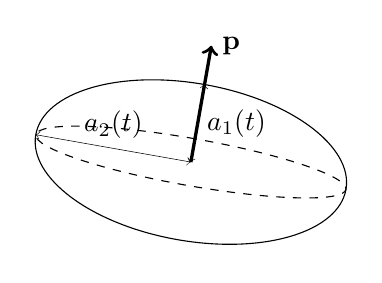
\begin{tikzpicture}[rotate=80]
        \draw(0,0) ellipse (1 cm and 2 cm);
        \draw[dashed](0,0) ellipse (0.3 cm and 2 cm);
        \draw[<->,very thin](0,0) --++ (1,0)node[midway,right]{$a_1(t)$};
        \draw[->,very thick](0,0) --++ (1.5,0)node[right]{$\textbf{p}$};
        \draw[<->,very thin](0,0) --++ (0,2)node[midway,above]{$a_2(t)$};
    \end{tikzpicture}
    \hfill
    \caption{Scheme of an  oblate spheroid oriented along the unit vector \textbf{p} with $a_1(t)$ and $a_2(t)$ the length of the semi axes of the spheroid.}
\end{figure}


\subsubsection*{The droplet internal velocity}

The internal velocity of a solid elastic particle following a homogeneous linear deformation can be described such as $\textbf{w}_2^0 = \bm\Gamma_\alpha \cdot \textbf{r}$ where we have introduced, $\bm\Gamma_\alpha$, the mean velocity gradient inside the particle, which symmetric part : $\textbf{E}_\alpha$, represents the rate of strain, and skew symmetric part : $\bm\Omega_\alpha$, represents the angular velocity. 
Even through the velocity fields $\textbf{w}_2^0 = \bm\Gamma_\alpha \cdot \textbf{r}$  can apply for liquid deforming droplet, an additional flow is present. 
Indeed, from the solution of the stokes equations we can predict the flow within a spherical isolated drop immersed in an unbounded fluid. 
Especially, we know that an solated droplet in translation exhibit internal motion known as Hill vortexes, see \ref{fig:flowlines} (b). 
For a drop immersed in an unbounded linear flow we can also derive an analytical solution such that $\textbf{w}_2^0 \sim \textbf{rrr}$, see \ref{fig:flowlines} (a). 
Therefore, the droplet's internal velocity fields is constituted with a component accounting for the complex internal motions that does not alter the shape of the drop, and another component that account for the linear deformation of the drop.  
\begin{figure*}
    \centering
    \begin{tikzpicture}
        \node (img3) at (0.6\textwidth,0) {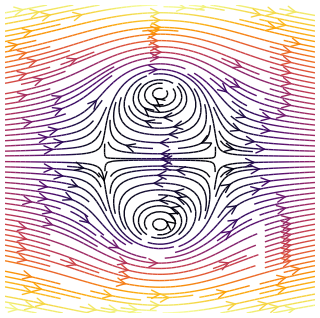
\includegraphics[width=0.3\textwidth,angle=270]{image/Rising_def_Stokes.png}};
        \node (img2) at (0.3\textwidth,0) {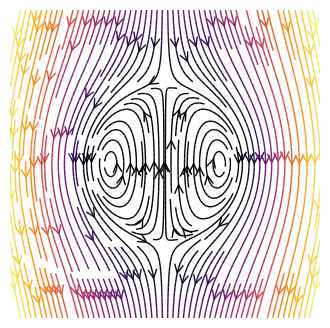
\includegraphics[width=0.3\textwidth]{image/Rising_Stokes.png}};
        % \draw (0.45\textwidth,0)node{$\rightarrow$};
        % \draw (0.45\textwidth,0.4cm)node{$\bm\Gamma_\alpha\cdot \textbf{r}$};
        \node (img1) at (0.0\textwidth,0) {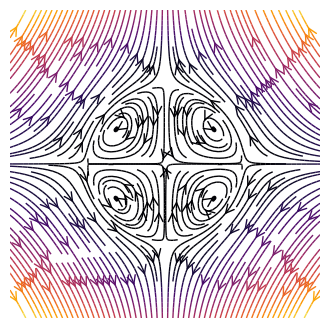
\includegraphics[width=0.3\textwidth]{image/Shear_Stokes.png}};
        \draw (img3.south)node{(c)};
        \draw (img2.south)node{(b)};
        \draw (img1.south)node{(a)};
    \end{tikzpicture}
    \caption{Three examples of steady state flow lines plots of an isolated droplet immersed into a viscous fluid. 
    (a) Rising sphere in uniform stokes flow (analytical solution in \ref{ap:Translating_sphere}). 
    (b) Fixed droplet in extensional flow (analytical solution in \ref{ap:Translating_sphere}).
    (c) Deformed droplet in rising motion (analytical solution of \citet{taylor1964deformation}). }
\end{figure*}
Consequently, the particle internal velocity might be written, 
\begin{equation}
    \textbf{w}_{2,i}^0(\textbf{x}_\alpha)
    = \bm\Gamma_{\alpha,ik}(t) \cdot \textbf{r}_k
    + \textbf{w}^{s}_{2,i}(t,\textbf{r})
    =\bm{\Omega}_{\alpha,ik}\cdot \textbf{r}_k
    + \textbf{E}_{\alpha,ik} \cdot \textbf{r}_k
    + \textbf{w}^{s}_{2,i}(t,\textbf{r})
\end{equation}
Where we introduced the vector $\textbf{w}^{s}_2(t,\textbf{r}) =\textbf{w}^{0}_{2,i}(t,\textbf{r})  - \bm\Gamma_{\alpha,ik}(t) \cdot \textbf{r}_k$ which represents all the internal motions that does not alter the drop's shape. 
Examples of such motions are displayed \ref{fig:flowlines}. 


From now on we consider that the internal velocity $\textbf{w}^{s}_2(t,\textbf{r})$ is not part of the particles unknown, but a function entirely determined by the particle and flow properties such that $\textbf{w}^{s}_2(t,\textbf{r}) =f_\textbf{w}(\textbf{u}_\alpha,\textbf{C}_\alpha,\bm\Gamma_\alpha,\textbf{u}_1,\bm \Gamma_1,\phi_2) $, where $\bm\Gamma_1 = \grad \textbf{u}_1$ and $\textbf{u}_1$ is the mean velocity fields evaluated at the particle position. 
As it is demonstrated in \ref{ap:Translating_sphere} the internal motion of an isolated spherical drop such as the one in \ref{eq:def_vel} might be determined theoretically from the relative motion and flow fields gradient in the limit of low Reynolds number.
We assume that such a relation exist for other regime. 
Consequently, The particle mean velocity gradient $\bm\Gamma_\alpha$ and its conformation tensor $\textbf C_\alpha$ are the only unknown of our problem. 
Therefore, we need to provide two equations, one for $\textbf{C}_\alpha$ and another for $\bm\Gamma_\alpha$. 

\subsubsection*{Kinematic and dynamic of a deformable spheroid}

The evolution of $\textbf{C}_\alpha$ and $\bm\Gamma_\alpha$ will be described by the second moment of mass and first moment of momentum equation.
Consequently, we must reformulate the terms in \ref{eq:dt_M_alpha} and \ref{eq:dt_P_alpha} in terms of $\textbf{C}_\alpha$ and $\bm\Gamma_\alpha$. 
The integrals constitutive of these moments equations can be written, 
\begin{align}
    \intO{(\textbf{rw}_2^0 )_{ij}+ (\textbf{w}_2^0 \textbf{r})_{ij}} 
    = \textbf{C}_{\alpha,ik} \cdot \bm\Gamma_{\alpha,kj}
    +  \bm\Gamma_{\alpha,ki} \cdot \textbf{C}_{\alpha,jk}
    +  \bm\Gamma_{\alpha,ij} + \bm\Gamma_{\alpha,ij}
    \\
    \intO{\rho_2 \textbf{w}_{2,i}^0\textbf{w}_{2,j}^0}
    = \frac{m_\alpha a^2}{5}[
        \bm\Gamma_{\alpha,lj}\bm\Gamma_{\alpha,ki} \textbf{C}_{\alpha,kl} 
        + \bm\Gamma_{\alpha,kj}\bm\Gamma_{\alpha,ki} 
        % + f_\textbf{ww}(\textbf{u}_\alpha,\textbf{C}_\alpha,\bm\Gamma_\alpha,\textbf{u}_1,\bm \Gamma_1,\phi_2)
        + f_\textbf{ww}(\textbf{u}_\alpha,\textbf{C}_\alpha,\bm\Gamma_\alpha,\textbf{u}_1,\bm \Gamma_1,\phi_2)
        ]
    \\
    \intO{\bm\sigma_{2,ij}^0}
    =
    % -\intO{p_2^0} \textbf{I}_{ij}
    \mu_2 v_\alpha [\bm\Gamma_{\alpha,ij} + \bm\Gamma_{\alpha,ij}
    + f_{\bm{\sigma}}(\textbf{u}_\alpha,\textbf{C}_\alpha,\bm\Gamma_\alpha,\textbf{u}_1,\bm \Gamma_1,\phi_2)]
    % + \textbf{I}_{ij}\intO{p_2^0} 
    \\
    \intS{\bm\sigma_{I,ij}^0}
    = \frac{2 \gamma v_\alpha }{a} \textbf{I}_{ij} - \frac{4 \gamma v_\alpha }{5 a} \textbf{C}_{\alpha,ij}
    +\mathcal(|\textbf{C}|^2)\\
    \intS{\textbf{r}\bm\sigma_1^0\cdot \textbf{n}_2}
    = 
    \frac{1}{2}\intS{(\textbf{r}\bm\sigma_1^0-\bm\sigma_1^0\textbf{r})\cdot \textbf{n}_2}
    + \frac{1}{2}\intS{(\textbf{r}\bm\sigma_1^0+\bm\sigma_1^0\textbf{r})\cdot \textbf{n}_2}
    % \textbf{M}(\textbf{u}_\alpha,\textbf{C}_\alpha,\bm\Gamma_\alpha,\textbf{u}_1,\bm \Gamma_1,\phi_2)
\end{align}
\tb{carry the actual decomposition with the velocity components }
\tb{mettre sous forme plus simple et expliquer l'osciallater sous forme 1d}
First, as discussed above only the deforming motion contribute to the symmetric part of the moment of momentum, we could therefore express it explicitly in terms of the particle unknown. 
Regarding the first moment of the surface tension, it has been computed analytically carrying a surface integral on the ellipsoidal surface of the droplet. 
Since, the droplets remain spheroidal under small deformation we choose to approximate $\intS{\bm\sigma_I^0}$ with its first order Taylor series in $\textbf{C}_\alpha$ without lost of generality.
Note that our expression of $\intS{\bm\sigma_I^0}$ is in agreement with \citet{lhuillier1987phenomenology} if one account for the slight difference of his definition of the deformation tensor which is half of $\textbf{C}_{\alpha}$. 
% in which our $\textbf{C}_\alpha$ is twice his, in the limit of small \textbf{C}_\alpha.
For the expression of $\intO{\rho_2 \textbf{w}_{2,i}^0\textbf{w}_{2,j}^0}$, $ \intO{\bm\sigma_{2,ij}^0}$ we had to introduce two unknown functions, $f_\textbf{ww}$, $f_{\bm{\sigma}}$, which vanish when $\textbf{w}^s_2 =0$. 
Therefore, these expressions are a sum of a function involving $\bm\Gamma_\alpha$ and an unknown part which depend on the parameters of the problem and need to be closed. 
The expression of $\intO{\rho_2 \textbf{w}_{2,i}^0\textbf{w}_{2,j}^0}$, $ \intO{\bm\sigma_{2,ij}^0}$ and $\intS{\textbf{r}\bm\sigma_1^0\cdot \textbf{n}_2}$ are very problem dependent. 
To provide a clearer example we computed these terms in \ref{ap:Translating_sphere} in the simplified scenario of an isolated droplet in a general linear flow. 

% The most common example is the expression for first moment \textbf{M}, which has been widely investigated in the pure straining situation, an example is given in \ref{ap:Translating_sphere} for spherical drop, and in \citet{raja2010inertial} for slightly deformable droplet in inertial flows. 
% It is important to notice that these functions are dependent of the relative drop-carrier fluid velocity, in such a way that the momentum and first moment of momentum are linked through the function $f_{\textbf{ww}},f_{\bm{\sigma}}$ and $\intS{\textbf{r}\bm\sigma_1^0\cdot \textbf{n}_2}$. 
% Indeed, even if it has been uniquely studied in pure linear flows, the relative motion of a particle might generate a first moment on its surface. 


At this point it wouldn't be wise trying to find an expression for each of these unknown functions in such a generality. 
Instead, we expose the unclosed set of equation of motions for spheroidal particles. 
In addition to the previously exposed equations (mass, momentum and energy equation) this system is constituted of three equations, one for $\textbf{C}_\alpha$ and two equation for the moment of momentum, the symmetric and skew-symmetric moment of momentum. 
% These read, 
\begin{align*}
    \ddt \textbf{C}_{\alpha,ij}
    = \textbf{C}_{\alpha,ik} \cdot \bm\Gamma_{\alpha,kj}
    +  \bm\Gamma_{\alpha,ki} \cdot \textbf{C}_{\alpha,jk},\\
    \frac{a^2  m_\alpha}{5} \ddt( \textbf{C}_{ik} \cdot \bm\Gamma_{\alpha,kj}
    -  \bm\Gamma_{\alpha,ki} \cdot \textbf{C}_{jk})
    =  \intS{(\textbf{r}\bm\sigma_2^0- \bm\sigma_2^0\textbf{r})\cdot \textbf{n}}\\
    \frac{m_\alpha a^2}{5}\ddt^2 \textbf{C}_\alpha
    - \frac{m_\alpha a^2}{5}[
    \bm\Gamma_{\alpha,lj}\bm\Gamma_{\alpha,ki} \textbf{C}_{\alpha,kl} + f_\textbf{ww}]
    + \mu_2 v_\alpha [(\bm \Gamma_{p,ij}+\bm \Gamma_{p,ji})
    + f_{\bm{\sigma}}]\\
    + \frac{2 \gamma v_\alpha }{a} \textbf{I}_{ij} 
    - \frac{4 \gamma v_\alpha }{5 a} (\textbf{C}_{ij} - \textbf{I}_{ij})
    = \intS{(\textbf{r}\bm\sigma_2^0+ \bm\sigma_2^0\textbf{r})\cdot \textbf{n}}
    % + \textbf{I}_{ij}\intO{p_2^0}
\end{align*}
% Where we placed the unknown function at the right hands side of these equations. 
Now, we would like to propose a more intuitive interpretation of the mass and momentum equations.
To that end, we make the problem dimensionless by introducing, 
the \textit{Capillary number} $Ca= \frac{\mu_1 U}{\gamma}$, The viscosity ratio $\lambda = \mu_2/\mu_1$, the density ratio $\zeta = \rho_2/\rho_1$ and the Reynolds number $Re = \frac{a U \rho_1}{\mu_1}$, with $U$ as the velocity scale. 
%  such that  $\bm\Gamma_\alpha'  = \frac{a}{U}\bm\Gamma$, and $\tau_a$ the timescale related to the drop shape evolution.
In the low Reynolds regime the first moment of surface traction forces will be proportional to a viscous stress (see \ref{ap:Translating_sphere}), therefore :$\intS{\textbf{r}\bm\sigma_2^0\cdot \textbf{n}} =\mu_1  \tau v_\alpha \intS{\textbf{r}\bm\sigma_2^0\cdot \textbf{n}}^*$, with $\tau$ the inverse timescale of the external solicitation.
The ratio between the external flow scale $\tau$ and the drop timescale $\tau_a$ is noted $\beta$. 
With that in mind, \ref{eq:dt_M_alpha}, \ref{eq:dt_mu_alpha} and \ref{eq:dt_S_alpha} might be written :
\begin{align}
    \beta \ddt \textbf{C}_{\alpha,ij}
    - \textbf{C}_{\alpha,ik} \cdot \bm\Gamma_{\alpha,kj}^*
    - \bm\Gamma_{\alpha,ki}^* \cdot \textbf{C}_{\alpha,jk},
    = 
    \bm\Gamma_{\alpha,ij}^*
    +  \bm\Gamma_{\alpha,ji}^*\\
    Re \zeta \beta \ddt( \textbf{C}_{\alpha,ik} \cdot \bm\Gamma_{\alpha,kj}^*
    -  \bm\Gamma_{\alpha,ki}^* \cdot \textbf{C}_{\alpha,jk}
    + \bm\Gamma_{\alpha,ji} - \bm\Gamma_{\alpha,ij})
    =  \intS{(\textbf{r}\bm\sigma_2^0- \bm\sigma_2^0\textbf{r})\cdot \textbf{n}}^*\\
    \zeta Re \frac{1}{5}  
    \left[
        \frac{1}{2}\beta^2 \ddt^2_* \textbf{C}_\alpha
        - \bm\Gamma_{\alpha,lj}^* \bm\Gamma_{\alpha,ki}^* \textbf{C}_{\alpha,kl}^* 
        - \bm\Gamma_{\alpha,kj}^* \bm\Gamma_{\alpha,ki}^* 
        - f_\textbf{ww}
    \right]\nonumber\\
    + \lambda \left[
        \beta \ddt \textbf{C}_{\alpha,ij}
        -\textbf{C}_{\alpha,ik} \cdot \bm\Gamma_{\alpha,kj}
        - \bm\Gamma_{\alpha,ki}^* \cdot \textbf{C}_{\alpha,jk},
        + f_{\bm{\sigma}}
    \right]\nonumber\\
    - \frac{1}{Ca}\left[
        \frac{4}{5} \textbf{C}_{\alpha,ij}
        +2 \textbf{I}_{ij} 
    \right]
    =
    \frac{1}{2}\intS{(\textbf{r}\bm\sigma_1^0+ \bm\sigma_1^0\textbf{r})\cdot \textbf{n}}^*
\end{align}
\tb{at this point it is not usefull to introduce the substitution in the last equaiton instead explain that it is proportional to the derivative in the limit}
The second moment of mass \ref{eq:dt_Cs}, is consistent with the equation found by \citet{goddard1967nonlinear} and \citet{lhuillier1987phenomenology}. 
Following, \citet{goddard1967nonlinear}  terminology, the left-hand side of \ref{eq:dt_Cs} is referred as the \textit{convected} derivative of $\textbf{C}^*_\alpha$. 
Therefore, the \textit{convected} derivative of $\textbf{C}_\alpha$ is equal to the rate of strain of the particle. 
The skew-symmetric part of the first moment of momentum \ref{eq:dt2_C}, it is basically the angular momentum balance of a non-spherical object. 
The right-hands side accounting for the external torque contribution. 
The symmetric part however has the form of a non-linear forced harmonic oscillatory equation for the droplet deformation. 
Indeed, the first groups of terms on the left-hand side represent the inertial contribution of the droplet internal fluid. 
It is made of a second order derivative plus non-linear terms in $\bm\Gamma_\alpha$. 
The second groups of terms is internal viscous contribution that arise directly from the definition of the stress \ref{eq:sigma_2_def}. 
It vanishes for small viscosity ration and is linear in the first derivative of $\textbf{C}_\alpha$. 
The last term on the left-hand side is the elastic response from the interface which is negligible for high capillary number $Ca \to \infty$. 
Then on right-hand side of the equation we find the first moment of surface force, $\intS{(\textbf{r}\bm\sigma_1^0+ \bm\sigma_1^0\textbf{r})\cdot \textbf{n}}^*$ which has an unknown expression at this stage. 
\ref{eq:dt2_C} might be regarded as a second order harmonic equation with non-linear contributions. 
However, the unknown function $f_\textbf{ww},\ f_{\bm{\sigma}}$ and $\intS{(\textbf{r}\bm\sigma_1^0+ \bm\sigma_1^0\textbf{r})\cdot \textbf{n}}^*$ are in general function of $\textbf{C}_\alpha$ and its higher derivatives of $\textbf{C}_\alpha$.   
Therefore, at this stage it is impossible to predict the nature of the harmonic regime followed by the droplet. 
To conclude on this matter one must find an expression for all this closure as well as determinate the impact of the non-linear terms.

We now examine the specific case studied by \citet{lamb1924hydrodynamics} where he considered no external contribution around the particle, therefore, $\intS{(\textbf{r}\bm\sigma_1^0+ \bm\sigma_1^0\textbf{r})\cdot \textbf{n}}^* = 0$.
It is found, that the amplitude of the second order harmonic mode of deformation, noted $\epsilon_2$, follows the second order partial differential equations,  
\begin{equation*}
    \ddt^2{\epsilon_2}
    + 2\lambda_2 \ddt \epsilon_2
    + \omega_2^2 \epsilon_2
     = 0,
\end{equation*}
where $\lambda_2$ and $\omega_2$ are the damping and frequency of coefficient defined as, 
\begin{align*}
    \lambda_2 = 5 \frac{\mu_2}{\rho_2a^2},
    && \omega_2 = \sqrt{8 \frac{\mu_2}{\rho_2 a^2}}.
\end{align*}
Where this equation has been obtained in the linear deformation regime for $\epsilon_2 \ll 1$. 
When multiplying \ref{eq:dt2_C} by, $\frac{10}{\zeta Re}$ we indeed find the exact same coefficient $\lambda_2$ and $\omega_2^2$ in front of, $\ddt \textbf{C}_{\alpha,ij}$ and $\textbf{C}_{\alpha,ij}$, respectively. 
In the limit of small $\textbf{C}_\alpha$, only these linear terms remain, therefore consistent with the reference work of \citet{lamb1924hydrodynamics}. 
\ref{eq:dt2_C} is somewhat more general than lamb's solution since it is expressed in an arbitrary reference frame. 
Which will prove to be useful in \ref{sec:Exemples} were we apply ensemble average on these quantities. 
However, with this equation we are able to describe only the second oscillatory mode. 
To study higher order modes one must use higher moment of momentum equations. 

In the past studies, the coupling between translational and oscillating nature of rising bubbles or droplets have been investigated \citet{lalanne2013effect}. 
For an isolated spherical droplet in translation through a stokes or potential flow we know that $
    f_\textbf{ww}
    = \frac{m_\alpha}{140 (\lambda +1)^2}
    (7 \textbf{u}_{\alpha 1} \textbf{u}_{\alpha 1} + \textbf{u}_{\alpha 1}\cdot \textbf{u}_{\alpha 1}\textbf{I})$, 
(see \ref{ap:Translating_sphere}). 
It is reasonable to guess that for a slightly spheroidal droplet in translation the expression might preserve the same form. 
Indeed, a coefficient related to $\textbf{C}_\alpha$ might appear in the expression nevertheless the overall contribution must be still proportional to $\textbf{u}_{\alpha 1} \textbf{u}_{\alpha 1}$. 
Likewise, for an inertial drops, it might be found that 
$\intS{(\textbf{r}\bm\sigma_1^0+ \bm\sigma_1^0\textbf{r})\cdot \textbf{n}}^* \sim A \textbf{u}_{\alpha 1} \textbf{u}_{\alpha 1} + B \textbf{u}_{\alpha 1} \cdot \textbf{u}_{\alpha 1}$ where $A$ and $B$ are constant. 
Indeed, the translational motion a spherical particle at slight inertia induce an overall unbalance stress on the surface of the particle generating a first moment \citet{taylor1964deformation}. 
The point is that the yet unknown closures, will help us bridge translational and drop's straining motions. 
Therefore, injecting these expressions into \ref{eq:dt2_C} would be a first step to accomplish a coupling between oscillating, or deforming motion with translating motion.
This is the subject of the last section. 
Obviously, now that we obtained a general formulation for the dynamic of the droplets' deformation, the most challenging aspect is to find expressions for closure terms. 


\subsubsection*{The particle internal energy balance.}

The surface of the particles, and internal kinetic energy can be written in this context as, 
\begin{align*}
    \beta \ddt \textbf{C}_{\alpha,ij}
    - \textbf{C}_{\alpha,ik} \cdot \bm\Gamma_{\alpha,kj}^*
    - \bm\Gamma_{\alpha,ki}^* \cdot \textbf{C}_{\alpha,jk},
    = 
    2\textbf{E}_{\alpha,ij}\\
    \intO{\rho_2 \textbf{w}_{2,i}^0\textbf{w}_{2,i}^0}
    = \frac{m_\alpha a^2}{5}[
        \bm\Gamma_{\alpha,li}\bm\Gamma_{\alpha,ki} \textbf{C}_{\alpha,kl} 
        + \bm\Gamma_{\alpha,ki}\bm\Gamma_{\alpha,ki} 
        + f_\textbf{ww}(\textbf{u}_\alpha,\textbf{C}_\alpha,\bm\Gamma_\alpha,\textbf{u}_1,\bm \Gamma_1,\phi_2)
        ]
    \\
    \intO{\bm\sigma_{2,ij}^0:\grad \textbf{u}_2^0}
    = 2 \mu_2 \intO{\textbf{e}_2^0:\textbf{e}_2^0}
    = 2\mu_2v_\alpha\left[ \textbf{E}_{\alpha,ij}\textbf{E}_{\alpha,ij}
    + f_{\textbf{e}}\right]\\
    % -\intO{p_2^0} \textbf{I}_{ij}
    \mu_2 v_\alpha [\textbf{E}_{\alpha,ij}
    + f_{\bm{\sigma}}(\textbf{u}_\alpha,\textbf{C}_\alpha,\bm\Gamma_\alpha,\textbf{u}_1,\bm \Gamma_1,\phi_2)]
    % + \textbf{I}_{ij}\intO{p_2^0} 
    \\
    s_\alpha \gamma
    = 
    \frac{3 \gamma v_\alpha }{a}\left[
        1
        + \frac{1}{20}\textbf{C}_\alpha:\textbf{C}_\alpha
    \right]
\end{align*}

\begin{equation}
    \ddt (W_\alpha + \gamma s_\alpha)
    + \intO{ \bm{\sigma}_2^0 : \grad\textbf{u}_2^0 }
    =\intS{\textbf{w}_1^0 \cdot \bm{\sigma}_1^0 \cdot \textbf{n}_2} 
\end{equation}

In conclusion, we have demonstrated how the first and second moment of momentum and mass equation can be used to describe the second mode oscillatory motion of a spheroidal drop in a Galilean reference frame. 
Therefore, the moment of momentum is a quantity of utmost importance for all kinds of particles with variable shape or volume.
This isn't limited to the momentum distribution, but all kind of properties can be described that way. 
In fact, if one wish to describe the first moment of the distribution of any local quantity $f_2^0$ and $f_I^0$ over the surface or volume of the particle, he must use the first moments' conservation equations. 
As an example, the mean concentration and distribution of surfactants on the bubbles' surface have a significant impact on the mass transfer rate between the dispersed and continuous phases.
In this case first moment of surfactant concentration could be considered here to track the evolution of the surfactant concentration and orientation over the particle surface, which would enable us to compute a better approximation of the drag force coefficient. 

% 
\section*{Re-derivation but more easy}
All these went way to complicated. 
So here is a more consize derivation that does keep track of the physics. 
We describe the geometry of the particle with the second moment of mass tensor, 
\begin{equation*}
    M_{\alpha,ij} 
    =\frac{m_\alpha a^2}{5} M_{\alpha,ij}^*
    = \frac{m_\alpha a^2}{5}\left[
        \left(
            \frac{a_1}{a}
        \right)^2 p_i p_j
        + 
        \left(
            \frac{a_1}{a}
        \right)^2(\delta_{ij}-  p_i p_j)
    \right]
\end{equation*}
This tensor has several notable properties, the volume conservation : $a_1 a_2^2 = a^3$ which means that $\textbf{M}_\alpha^*$ has two eigenvalues linked through $M^1 = (M^2)^{-2}$ or $M^2 = (M^1)^(-1/2)$. 
At small deformation, i.e. $M_1 - 1\ll 1$ we therefore have $M^1 = 1 - (M^1-1)/2$.
This ultimately means that at small deformation the trace is a constant namely $M_{ij} \delta_{ij} = 3+\mathcal{O}((M^1 -1)^2)$. 




Let's now reformulate the integral of the problem namely, 
\begin{align}
    \intO{(\textbf{rw}_ 2^0 )_{ij}+ (\textbf{w}_2^0 \textbf{r})_{ij}} 
    = \textbf{M}_{\alpha,ik} \cdot \bm\Gamma_{\alpha,jk}
        +  \bm\Gamma_{\alpha,ik} \cdot \textbf{M}_{\alpha,jk}
    \\
    \intO{\rho_2 \textbf{w}_{2,i}^0\textbf{w}_{2,j}^0}
    = \bm\Gamma_{\alpha,jl}\bm\Gamma_{\alpha,ik} \textbf{M}_{\alpha,kl}  
        +\intO{\rho_2 \textbf{w}_{2,i}^s\textbf{w}_{2,j}^s}
    \\
    \intO{\bm\sigma_{2,ij}^0}
    =
    2 \mu_2 v_\alpha \textbf{E}_{\alpha,ij}
    - \intO{p_2^0} \textbf{I}_{ij}
    + \mu_2 \intS{(\textbf{n}_i \textbf{w}_{2,j}^s + \textbf{n}_j \textbf{w}_{2,i}^s)}
    \\
    \intS{\bm\sigma_{I,ij}^0}
    = \frac{\gamma v_\alpha }{a} \left[
        2\textbf{I}_{ij} 
        - \frac{4  }{5} (\textbf{M}_{\alpha,ij}^* - \textbf{I}_{\alpha,ij})
    \right]
    +\mathcal(O)(\textbf{C}\cdot \textbf{C})\\
    s_\alpha 
    = 4\pi a^2 (1+\frac{\textbf{C}:\textbf{C}}{15})
\end{align}
for the surface tension term is made of two terms, one corresponding to Laplace pressure and the other to the deviatoric stress. 




The equation for the orientation, second moment of mass torque, symmetric moment of momentum and trace of the moment of momentum reads, 
\begin{align*}
    \ddt \textbf{pp}_{\alpha,ij}
    = \textbf{pp}_{\alpha,ik} \cdot \bm\Omega_{\alpha,jk}
    +  \bm\Omega_{\alpha,ik} \cdot \textbf{pp}_{\alpha,jk}\\
    \ddt \textbf{M}_{\alpha,ij}
    = \textbf{M}_{\alpha,ik} \cdot \bm\Gamma_{\alpha,jk}
    +  \bm\Gamma_{\alpha,ik} \cdot \textbf{M}_{\alpha,jk}\\
    \ddt (\textbf{I}_{\alpha,ik}\bm\omega_{\alpha,k} )
    = 
    \intS{(\textbf{r}\times\bm\sigma_1^0\cdot \textbf{n})_i} \\
    \frac{1}{2}\ddt^2 \textbf{M}_{\alpha,ij}
    -  \bm\Gamma_{\alpha,jl}\bm\Gamma_{\alpha,ik} \textbf{M}_{\alpha,kl}  
    + 2 \mu_2 v_\alpha \textbf{E}_{\alpha,ij}
    + \frac{\gamma v_\alpha }{a} \left[
    2\textbf{I}_{ij} 
    - \frac{4 \gamma v_\alpha }{5 a} (\textbf{M}_{\alpha,ij}^* - \textbf{I}_{\alpha,ij})
    \right]\\
    = 
    \frac{1}{2}\intS{(\textbf{r}\bm\sigma_1^0 + \bm\sigma_1^0\textbf{r})\cdot \textbf{n}} 
    + \intO{\rho_2 \textbf{w}_{2,i}^s\textbf{w}_{2,j}^s}
    + \intO{p_2^0} \textbf{I}_{ij}
    - \mu_2 \intS{(\textbf{n}_i \textbf{w}_{2,j}^s + \textbf{n}_j \textbf{w}_{2,i}^s)}\\
    % \frac{1}{2}\ddt^2 \textbf{M}_{\alpha,mm}
    -  \bm\Gamma_{\alpha,ml}\bm\Gamma_{\alpha,mk} \textbf{M}_{\alpha,kl}  
    + \frac{\gamma v_\alpha }{a} 
    % \left[
    2\textbf{I}_{mm} 
    % - \frac{4 }{5 } (\textbf{M}_{\alpha,mm}^* - \textbf{I}_{\alpha,mm})
    % \right]
    % \\
    = 
    \intS{\textbf{r}_m\cdot\bm\sigma_{1,mk}^0\cdot \textbf{n}_k} 
    + \intO{\rho_2 \textbf{w}_{2,m}^s\cdot \textbf{w}_{2,m}^s}
    + \intO{p_2^0} \textbf{I}_{mm}
\end{align*}

As the derivative of $M_{ij}$ in these equations actually takes in account the change of orientation of the particle it might be useful to re-derive these equations in the eigenbasis of the matrix $M_{ij}$

To the first order in deformation the deviatoric part reads, 
\begin{align*}
    \frac{1}{2}\ddt^2 \textbf{M}_{\alpha,ij}
    -   \textbf{M}_{\alpha,kl} 
    (\bm\Gamma_{\alpha,jl}\bm\Gamma_{\alpha,ik}  
    - \frac{1}{3}
    \bm\Gamma_{\alpha,ml}\bm\Gamma_{\alpha,mk}  
    \textbf{I}_{ij}
    )
    + 2 \mu_2 v_\alpha \textbf{E}_{\alpha,ij}
    - \frac{\gamma v_\alpha }{a} 
    \frac{4  }{5} (\textbf{M}_{\alpha,ij}- \textbf{I}_{ij})
    \\
    = 
    \frac{1}{2}\intS{(\textbf{r}\bm\sigma_1^0 + \bm\sigma_1^0\textbf{r} - \frac{2}{3}\textbf{r}\cdot \bm\sigma_1^0 \textbf{I})\cdot \textbf{n}} 
    + \intO{\rho_2 (\textbf{w}_{2,i}^s\textbf{w}_{2,j}^s - \frac{1}{3}\textbf{w}_{2,m}^s\textbf{w}_{2,m}^s \textbf{I}_{ij}) }
    - \mu_2 \intS{(\textbf{n}_i \textbf{w}_{2,j}^s + \textbf{n}_j \textbf{w}_{2,i}^s)}\\
\end{align*}
It can be somewhat useful to extract the proportionality coefficient of each terms. 
Denotining dimensionless qte by a $*$ we have, 
\begin{align*}
    \frac{\rho_2 a^2}{5 \tau^2}\left[\frac{1}{2}\ddt^2 \textbf{M}_{\alpha,ij}^*
    -  \bm\Gamma_{\alpha,jl}^*\bm\Gamma_{\alpha,ik}^* \textbf{M}_{\alpha,kl}^*
    \right]  
    + \frac{2 \mu_2  }{\tau} \textbf{E}_{\alpha,ij}^*
    + \frac{\gamma  }{a} \left[
    2\textbf{I}_{ij} 
    - \frac{4 }{5} (\textbf{M}_{\alpha,ij}^* - \textbf{I}_{\alpha,ij})
    \right]\\
    = 
    \frac{1}{2}\intS{(\textbf{r}\bm\sigma_1^0 + \bm\sigma_1^0\textbf{r})\cdot \textbf{n}} 
    + \intO{\rho_2 \textbf{w}_{2,i}^s\textbf{w}_{2,j}^s}
    + \intO{p_2^0} \textbf{I}_{ij}
    - \mu_2 \intS{(\textbf{n}_i \textbf{w}_{2,j}^s + \textbf{n}_j \textbf{w}_{2,i}^s)}\\
\end{align*}

The forcing terms are really problem dependent. 
Thus, at this stage it cannot be scaled in terms of timescale. 

In order to be more consis, we may write :
\begin{align*}
    \textbf{F}_{ij}(\textbf{w}^s,\bm\sigma_1^0)
    = 
    \frac{1}{2}\intS{(\textbf{r}\bm\sigma_1^0 + \bm\sigma_1^0\textbf{r} - \frac{2}{3}\textbf{r}\cdot \bm\sigma_1^0 \textbf{I})\cdot \textbf{n}} 
    + \intO{\rho_2 (\textbf{w}_{2,i}^s\textbf{w}_{2,j}^s - \frac{1}{3}\textbf{w}_{2,m}^s\textbf{w}_{2,m}^s \textbf{I}_{ij}) }
    - \mu_2 \intS{(\textbf{n}_i \textbf{w}_{2,j}^s + \textbf{n}_j \textbf{w}_{2,i}^s)}\\
\end{align*} 
Indicating that the forcing term is related to the exterior contribution and the external stresses. 

\begin{align*}
    \ddt^2 \textbf{M}_{\alpha,ij}^*
    -2  \textbf{M}_{\alpha,kl}^* 
    (\bm\Gamma_{\alpha,jl}^*\bm\Gamma_{\alpha,ik}^*  
    - \frac{1}{3}
    \bm\Gamma_{\alpha,ml}^*\bm\Gamma_{\alpha,mk}^*  
    \textbf{I}_{ij}
    )
    + \frac{10 \mu_2 \tau}{ \rho_2 a^2} 2\textbf{E}_{\alpha,ij}^*
    - 8 \frac{\tau^2 \gamma  }{\rho_2 a^3} 
     (\textbf{M}_{\alpha,ij}^*- \textbf{I}_{ij})\\
    = 
    \frac{\tau^2 10}{a^2 m_\alpha}
    \left[\textbf{F}_{\sigma_1, ij}
    + \textbf{F}_{ww, ij}
    + \textbf{F}_{\sigma_2, ij}\right]
\end{align*}

All these unclose term are really problem dependent, for now all we now is that at low Reynolds number we are in the viscous regime, besides this external flow that drives these scales. 
Meaning that, 
\begin{align*}
    \intO{\rho_2 \textbf{w}_{2,i}^0\textbf{w}_{2,j}^0}
    \sim \frac{m_\alpha a^2}{\tau_u^2} \textbf{F}_{ww}^*
    \\
    \mu_2 \intS{(\textbf{n}_i \textbf{w}_{2,j}^s + \textbf{n}_j \textbf{w}_{2,i}^s)}
    \sim \frac{v_\alpha \mu_2}{\tau_u} \textbf{F}_{e}^*
    \\
    \intS{\bm\sigma_1^0 \textbf{rn}}
    \sim 
    \frac{v_\alpha \mu_1}{\tau_u} \textbf{F}_{\sigma}^*
\end{align*} 

\begin{align*}
    \ddt^2 \textbf{M}_{\alpha,ij}^*
    -2  \textbf{M}_{\alpha,kl}^* 
    (\bm\Gamma_{\alpha,jl}^*\bm\Gamma_{\alpha,ik}^*  
    - \frac{1}{3}
    \bm\Gamma_{\alpha,ml}^*\bm\Gamma_{\alpha,mk}^*  
    \textbf{I}_{ij}
    )
    + \frac{10 \mu_2 \tau}{ \rho_2 a^2} 2\textbf{E}_{\alpha,ij}^*
    - 8 \frac{\tau^2 \gamma  }{\rho_2 a^3} 
     (\textbf{M}_{\alpha,ij}^*- \textbf{I}_{ij})\\
    = 
    \frac{\tau^2 10 \mu_1 }{a^2 \rho_2 \tau_u}
    \textbf{F}_{\sigma_1, ij}
    + \frac{\tau^2 10}{\tau_u^2} \textbf{F}_{ww, ij}
    + \frac{\tau^2 10 \mu_1 }{a^2 \rho_2 \tau_u} \textbf{F}_{\sigma_2, ij}
\end{align*}


\subsubsection*{Re-derivation but with dimensionless scaling}

\begin{align}
    \intO{(\textbf{rw}_ 2^0 )_{ij}+ (\textbf{w}_2^0 \textbf{r})_{ij}} 
    = \textbf{M}_{\alpha,ik} \cdot \bm\Gamma_{\alpha,jk}
        +  \bm\Gamma_{\alpha,ik} \cdot \textbf{M}_{\alpha,jk}
    \\
    \intO{\rho_2 \textbf{w}_{2,i}^0\textbf{w}_{2,j}^0}
    = \bm\Gamma_{\alpha,jl}\bm\Gamma_{\alpha,ik} \textbf{M}_{\alpha,kl}  
        +\intO{\rho_2 \textbf{w}_{2,i}^s\textbf{w}_{2,j}^s}
    \\
    \intO{\bm\sigma_{2,ij}^0}
    =
    2 \mu_2 v_\alpha \textbf{E}_{\alpha,ij}
    - \intO{p_2^0} \textbf{I}_{ij}
    + \mu_2 \intS{(\textbf{n}_i \textbf{w}_{2,j}^s + \textbf{n}_j \textbf{w}_{2,i}^s)}
    \\
    \intS{\bm\sigma_{I,ij}^0}
    = \frac{\gamma v_\alpha }{a} \left[
        2\textbf{I}_{ij} 
        - \frac{4  }{5} (\textbf{M}_{\alpha,ij}^* - \textbf{I}_{\alpha,ij})
    \right]
    +\mathcal(O)(\textbf{C}\cdot \textbf{C})\\
    s_\alpha 
    = 4\pi a^2 (1+\frac{\textbf{C}:\textbf{C}}{15})
\end{align}

Then, 
\begin{align*}
    \frac{\rho_2 a^2}{5}\left[
        \frac{1}{\tau^2}\frac{1}{2}\ddt^2 \textbf{M}_{\alpha,ij}
    -   \frac{1}{\tau^2}\bm\Gamma_{\alpha,jl}\bm\Gamma_{\alpha,ik} \textbf{M}_{\alpha,kl}  
    - \frac{1}{\tau_u^2} \textbf{F}_{ww}^*
    \right]\\
    + \mu_2  \left[
        \frac{1}{\tau} 2\textbf{E}_{\alpha,ij}
    + \frac{1}{\tau_u} \textbf{F}_\sigma^*
    \right]\\
    + \frac{\gamma  }{a} \left[
    2\textbf{I}_{ij} 
    - \frac{4  }{5} (\textbf{M}_{\alpha,ij}^* - \textbf{I}_{\alpha,ij})
    \right]\\
    = 
    \frac{1}{2}
    \frac{ \mu_1}{\tau_u} 
    \textbf{F}_{\sigma_1}^*
    % \intS{(\textbf{r}\bm\sigma_1^0 + \bm\sigma_1^0\textbf{r})\cdot \textbf{n}} 
    % + \intO{p_2^0} \textbf{I}_{ij}
\end{align*}

which then, 
\begin{align*}
    \frac{\rho_2}{\rho_1}\frac{\rho_1 a^2}{5\mu_1\tau_u}\left[
        \frac{\tau_u^2}{\tau^2}\frac{1}{2}\ddt^2 \textbf{M}_{\alpha,ij}
    -   \frac{\tau_u^2}{\tau^2}\bm\Gamma_{\alpha,jl}\bm\Gamma_{\alpha,ik} \textbf{M}_{\alpha,kl}  
    - \textbf{F}_{ww}^*
    \right]\\
    + \frac{\mu_2}{\mu_1}  \left[
        \frac{\tau_u}{\tau} 2\textbf{E}_{\alpha,ij}
    +  \textbf{F}_\sigma^*
    \right]\\
    + \frac{\gamma \tau_u }{a\mu_1} \left[
    2\textbf{I}_{ij} 
    - \frac{4  }{5} (\textbf{M}_{\alpha,ij}^* - \textbf{I}_{\alpha,ij})
    \right]\\
    = 
    \frac{1}{2}
    \textbf{F}_{\sigma_1}^*
    % \intS{(\textbf{r}\bm\sigma_1^0 + \bm\sigma_1^0\textbf{r})\cdot \textbf{n}} 
    % + \intO{p_2^0} \textbf{I}_{ij}
\end{align*}

In terms of dimensionless groups
\begin{align*}
    \zeta Re\left[
        \beta^2 \frac{1}{2}\ddt^2 \textbf{M}_{\alpha,ij}
    -   \beta^2 \bm\Gamma_{\alpha,jl}\bm\Gamma_{\alpha,ik} \textbf{M}_{\alpha,kl}  
    - \textbf{F}_{ww}^*
    \right]\\
    + \lambda  \left[
        \beta 2\textbf{E}_{\alpha,ij}
    +  \textbf{F}_\sigma^*
    \right]\\
    + \frac{1}{Ca} \left[
    2\textbf{I}_{ij} 
    - \frac{4  }{5} (\textbf{M}_{\alpha,ij}^* - \textbf{I}_{\alpha,ij})
    \right]\\
    = 
    \frac{1}{2}
    \textbf{F}_{\sigma_1}^*
    % \intS{(\textbf{r}\bm\sigma_1^0 + \bm\sigma_1^0\textbf{r})\cdot \textbf{n}} 
    % + \intO{p_2^0} \textbf{I}_{ij}
\end{align*}


\subsubsection*{Slow flows wheer beta equal 0 }

\textbf{Steady state equillibrium }
\begin{align*}
    - \zeta Re \textbf{F}_{ww}^*
    + \lambda  \textbf{F}_\sigma^*
    + \frac{1}{Ca} \left[
    2\textbf{I}_{ij} 
    - \frac{4  }{5} (\textbf{M}_{\alpha,ij}^* - \textbf{I}_{\alpha,ij})
    \right]
    = 
    \frac{1}{2}
    \textbf{F}_{\sigma_1}^*
    % \intS{(\textbf{r}\bm\sigma_1^0 + \bm\sigma_1^0\textbf{r})\cdot \textbf{n}} 
    % + \intO{p_2^0} \textbf{I}_{ij}
\end{align*}

In the last part i want to be able to neglect all the components on the left

if the reynolds number is indeed negligible we have 

\begin{align*}
    + \lambda  \textbf{F}_\sigma^*
    + \frac{1}{Ca} \left[
    2\textbf{I}_{ij} 
    - \frac{4  }{5} (\textbf{M}_{\alpha,ij}^* - \textbf{I}_{\alpha,ij})
    \right]
    = 
    \frac{1}{2}
    \textbf{F}_{\sigma_1}^*
    % \intS{(\textbf{r}\bm\sigma_1^0 + \bm\sigma_1^0\textbf{r})\cdot \textbf{n}} 
    % + \intO{p_2^0} \textbf{I}_{ij}
\end{align*}
which give the equillibrium of surface tension internal / external stresses
This must be respected for almost all steady state equilibrium presented in appendix
It is clear that if either $\lambda = 0$ or that we are looking for the fluid phase stress then the int on the left vanish. 
And we are left with an equillibrium between surface tension and stresslet

\tb{In this regime one might recognize Laplace law}

\textbf{Drop in air }
\begin{align*}
    \zeta Re\left[
         \frac{1}{2}\ddt^2 \textbf{M}_{\alpha,ij}
    -    \bm\Gamma_{\alpha,jl}\bm\Gamma_{\alpha,ik} \textbf{M}_{\alpha,kl}  
    \right]
    +   
        \frac{\lambda}{\beta} 2\textbf{E}_{\alpha,ij}
    + \frac{1}{Ca\beta^2} \left[
    2\textbf{I}_{ij} 
    - \frac{4  }{5} (\textbf{M}_{\alpha,ij}^* - \textbf{I}_{\alpha,ij})
    \right]\\
    = 
    0 
\end{align*}
Indeed, in this case we still consier that the surface tension is comparable with the ratio of time scale of course. 
Besides, 
\tb{In this regime one might recognize Lamb's equation }



\subsubsection*{The local basis equation}

Any second order tensor $\textbf{A}$ can be express in the vector $\{\textbf{p}^1,\textbf{p}^2,\textbf{p}^3\}$ which form an orthonormal basis. 
Indeed, 
\begin{equation}
    A_{ij}
    = 
    A^{ab}
    p_i^a
    p_j^b
\end{equation}
with, $A^{ab}$ the components of \textbf{A} in the basis $\{\textbf{p}^1,\textbf{p}^2,\textbf{p}^3\}$. 
These components can be obtained through the operation, 
\begin{equation*}
    A_{ij} 
    p_i^a
    p_j^b
    = 
    A^{cd}
    p_i^c
    p_j^d
    p_i^a
    p_j^b
    = 
    A^{ab}
\end{equation*}
From there it is easy to understand that to obtain the evolution equation in the eigenbasis one has to multiply the previous set of equation with $p_i^ap_j^b$. 

Some properties of the change of basis must be stated. 
If, 
\begin{equation}
    \Omega_{ij} = \frac{1}{2} [A_{ij}-A_ji]
\end{equation}
Then, 
\begin{equation}
    \Omega^{ab} = \frac{1}{2} [A^{ba}-A^{ab}]
\end{equation}
Since, 
\begin{equation}
    \Omega_{ij} = \frac{1}{2} [A^{ab} p^a_i p^b_j-A^{ba} p^b_j p^a_i]
    =  \frac{1}{2} [A^{ab} - A_{ba} ]p^b_j p^a_i
    =  \Omega^{ab} p^b_j p^a_i
\end{equation}
where $\bm\Omega$ is a skew symmetric tensor. 


Since all the $\textbf{p}^a$ rotate according to the same angular velocity we can write, $\ddt p_i^a =\Omega_{ik} p_k^a$, and more generally, 
\begin{equation*}
    \ddt(p_i^ap_j^b)
    = 
    \Omega_{ik} p_k^ap_j^b
    + \Omega_{jk} p_i^ap_k^b
\end{equation*}
with this equation one is able to reformulate any equation of the system above.
To get the second derivative of this tensor we can directly carry out the operation,  
\begin{align*}
    \ddt\ddt(p_i^ap_j^b)
    = 
    \ddt (\Omega_{ik} p_k^ap_j^b)
    + \ddt (\Omega_{jk} p_i^ap_k^b)\\
    = 
    \dot{\Omega}_{ik} p_k^ap_j^b
    + \dot{\Omega}_{jk} p_i^ap_k^b
    + (
        \Omega_{kl} p_l^ap_j^b
    + \Omega_{jl} p_k^ap_l^b
    )\Omega_{ik}
    + (\Omega_{il} p_l^ap_k^b
    + \Omega_{kl} p_i^ap_l^b)\Omega_{jk}\\
    = 
    \dot{\Omega}_{ik} p_k^ap_j^b
    + \dot{\Omega}_{jk} p_i^ap_k^b
    + \Omega_{ik}\Omega_{kl} p_l^ap_j^b
    + \Omega_{ik}\Omega_{jl} p_k^ap_l^b
    + \Omega_{jk}\Omega_{il} p_l^ap_k^b
    + \Omega_{jk}\Omega_{kl} p_i^ap_l^b\\
\end{align*}

Multiplying the equation for \textbf{M} by $\textbf{PP}$ reads, 
\begin{equation*}
    \ddt M^{ab}
    = 
    M^{ac} E^{bc} 
    + E^{ac} M^{bc}
\end{equation*}

The stresslet equation can be written by the same operation but first notice that, 
\begin{align}
    p_i^ap_j^b\ddt^2 M_{ij}
    = 
    \ddt( p_i^ap_j^b \ddt M_{ij})
    - \ddt (p_i^ap_j^b )\ddt M_{ij}\\
    = 
    \ddt( \ddt (p_i^ap_j^b M_{ij}))
    - \ddt(   M_{ij} \ddt  p_i^ap_j^b )
    - \ddt (p_i^ap_j^b )\ddt M_{ij}\\
    = 
    \ddt^2 M^{ab}
    - 2 \ddt (p_i^ap_j^b) \ddt M_{ij}
    - M_{ij} \ddt^2 (p_i^ap_j^b)
    \\
\end{align}
Also, 

The second term reads, 
\begin{align*}
    M_{ij} \ddt^2 (p_i^ap_j^b)
    = M^{cb} \dot{\Omega}^{ca}
    + M^{ac} \dot{\Omega}^{cb}
    + M^{cd} \Omega^{ca}\Omega^{db}
    + M^{cd} \Omega^{ca}\Omega^{db}
    + M^{cb} \Omega^{cd}\Omega^{da} 
    + M^{ac} \Omega^{cd}\Omega^{db} \\
\end{align*}
Must figure out if $\textbf{M}\cdot\bm\Omega$ vanish in the local basis. 
Also, 
\begin{align*}
    \ddt (p_i^ap_j^b) \ddt M_{ij}
    = 
    (\Omega_{ik} p_k^ap_j^b
    + \Omega_{jk} p_i^ap_k^b)
    (M_{il} \Gamma_{jl}
    +  \Gamma_{il} M_{jl})\\
    = 
    + M_{cd}\Omega_{ca} \Gamma_{bd}   
    + M_{cd}\Omega_{db} \Gamma_{ac}   
    + M_{bd}\Omega_{ca} \Gamma_{cd}  
    + M_{ad}\Omega_{cb}  \Gamma_{cd} 
\end{align*}
Some terms of this expression might eventually cancel out with the previous one.
But before let's compute the second inertial term, 
\begin{align*}
    p_i^a p_j^b M_{kl}( \Gamma_{jl}\Gamma_{ik} 
    - \frac{1}{3}
    \Gamma_{ml}\Gamma_{mk}  
    {I}_{ij})
    = 
    M^{cd} \Gamma^{bd}\Gamma^{ac} 
    - \frac{1}{3}
    M^{cd}\Gamma^{ed}\Gamma^{ec}  
    \delta^{ab}
\end{align*}
Now we need a way to simplify these equations. 
This is done by noticing that $M^{ab}$ and $E^{ab}$ are actually diagonal tensors. 

The sum of these terms yields, 
\begin{align*}
    - \frac{1}{2}(
    M^{cb} \dot{\Omega}^{ca}
    + M^{ac} \dot{\Omega}^{cb}
    + M^{cd} \Omega^{ca}\Omega^{db}
    + M^{cd} \Omega^{ca}\Omega^{db}
    + M^{cb} \Omega^{cd}\Omega^{da} 
    + M^{ac} \Omega^{cd}\Omega^{db}
)\\
    - M^{cd}\Omega^{ca} \Gamma^{bd}   
    - M^{cd}\Omega^{db} \Gamma^{ac}   
    - M^{bd}\Omega^{ca} \Gamma^{cd}  
    - M^{ad}\Omega^{cb}  \Gamma^{cd} 
    - M^{cd}( \Gamma^{bd}\Gamma^{ac} 
    - \frac{1}{3}
    \Gamma^{ed}\Gamma^{ec}  
    \delta^{ab})\\
    = 
    -\frac{1}{2}(
    M^{cb} \dot{\Omega}^{ca}
    + M^{ac} \dot{\Omega}^{cb}
    + M^{ac} \Omega^{dc} \Omega^{db}  
    + M^{bd} \Omega^{cd}  \Omega^{ca}
    + 2 M^{ac} E^{dc} \Omega^{db}  
    + 2 M^{bd} E^{cd} \Omega^{ca}
    )\\
    - M^{cd} E^{ac} E^{bd} 
    + \frac{1}{3} M^{cd}
    \Gamma^{ed}\Gamma^{ec}  
    \delta^{ab}
\end{align*}

Applying these changes the stress let equation reads, 
\begin{align*}
    \frac{1}{2}\ddt^2 M^{ab}
    -\frac{1}{2}(
        M^{cb} \dot{\Omega}^{ca}
        + M^{ac} \dot{\Omega}^{cb}
        + M^{ac} \Omega^{dc} \Omega^{db}  
        + M^{bd} \Omega^{cd}  \Omega^{ca}
        + 2 M^{ac} E^{dc} \Omega^{db}  
        + 2 M^{bd} E^{cd} \Omega^{ca}
        )\\
        - M^{cd} E^{ac} E^{bd} 
        - \frac{1}{3} M^{cd}
        \Gamma^{ed}\Gamma^{ec}  
        \delta^{ab}
    + 2 \mu_2 v_\alpha E^{ab}
    - \frac{\gamma v_\alpha }{a} 
    \frac{4  }{5} (M^{ab} - \delta^{ab})
    = \textbf{F}^{ab}(\textbf{w}^s,\bm\sigma_1^0)
\end{align*}
The terms that remains when $a=b$ are, 
\begin{align*}
    \frac{1}{2}\ddt^2 M^{ab}
    - M^{ac} \Omega^{dc} \Omega^{db}  
    - M^{cd} E^{ac} E^{bd} 
    + \frac{1}{3} M^{cd}
    \Gamma^{ed}\Gamma^{ec}  
    \delta^{ab}
    + 2 \mu_2 v_\alpha E^{ab}
    - \frac{\gamma v_\alpha }{a} 
    \frac{4  }{5} (M^{ab} - \delta^{ab})
    = \textbf{F}^{ab}(\textbf{w}^s,\bm\sigma_1^0)
\end{align*}
with the mass equation, 
\begin{align*}
    \ddt M^{ab}
    = 2 E^{ab}M^{ab}
\end{align*}
The terms that does not remain when $a\neq b$ are, 
\begin{align*}
    -\frac{1}{2}(
        M^{cb} \dot{\Omega}^{ca}
        + M^{ac} \dot{\Omega}^{cb}
        + M^{ac} \Omega^{dc} \Omega^{db}  
        + M^{bd} \Omega^{cd}  \Omega^{ca}
        )
    = \textbf{F}^{ab}(\textbf{w}^s,\bm\sigma_1^0)
\end{align*}
\subsection{Oblate spheroidal fluid particles}

Many studies have been conducted to determine the influence of the droplets' deformation on suspension Rheology \citet{goddard1967nonlinear,lhuillier1987phenomenology,maffettone1998equation}.
Most of the authors considered the Rheology of such an emulsion for neutrally buoyant droplets in linear flows. 
In this work, we would like to present a more general framework in which we consider the deformation of droplet's in arbitrary flows. 
In this section we first describe the behavior of a single deformable drop. 
Latter in this paper we present the influence of such a deformation on the suspension rheology. 
At this stage the only restriction that we make about the drop is that it possesses oblate spheroidal shape. 
This is consistent with shape that adopt buoyant droplets or bubbles rising in a Newtonian fluid. 

\subsubsection*{Shape description of the droplet}
We consider oblate spheroidal droplets as it is depicted \ref{fig:scheme_spheroid}. 
\begin{figure}[h!]
    \centering
    \hfill
    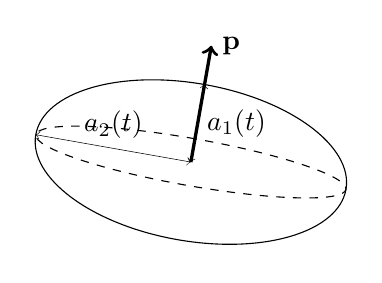
\begin{tikzpicture}[rotate=80]
        \draw(0,0) ellipse (1 cm and 2 cm);
        \draw[dashed](0,0) ellipse (0.3 cm and 2 cm);
        \draw[<->,very thin](0,0) --++ (1,0)node[midway,right]{$a_1(t)$};
        \draw[->,very thick](0,0) --++ (1.5,0)node[right]{$\textbf{p}$};
        \draw[<->,very thin](0,0) --++ (0,2)node[midway,above]{$a_2(t)$};
    \end{tikzpicture}
    \hfill
    \caption{Scheme of an  oblate spheroid oriented along the unit vector \textbf{p} with $a_1(t)$ and $a_2(t)$ the length of the semi axes of the spheroid.
    Note that when the drop is spherical we have $a_1=a_2=a$}
    \label{fig:scheme_spheroid}
\end{figure}
This shape might be described completely by the second moment of mass, $\textbf{M}_\alpha$.
In this context, each eigenvalue of the second moment of mass tensor is proportional to square semi axes of the particle. 
Indeed, by direct integration over the spheroidal particle volume we may find :
\begin{equation*}
    \textbf{M}_\alpha
    = \frac{m_\alpha a^2}{5}\left[
        \left(\frac{a_1}{a}\right)^2\textbf{pp}
        + \left(\frac{a_2}{a}\right)^2 (\textbf{I} - \textbf{pp}),
    \right] 
\end{equation*}
Additionally, note that due to the volume conservation condition we have : $ a_2^2 a_1 = a^3$. 
This means that : $M_1 = M_2^{-2}$, where the $M_i$ are the eigenvalues of the dimensionless tensor $\frac{m_\alpha a^2}{5}\textbf{M}_\alpha^* = \textbf{M}_\alpha$. 
Note that if we consider small deformations, meaning $M_1 - 1 \ll 1$ we have $M_1  = M_2^{-2} = 1 - 2 (M_2 - 1) + \mathcal{O}((M_2 -1)^2)$. 
Consequently, for small deformation the trace of the second moment of mass tensor reads :  $\frac{1}{3}\textbf{I}:\textbf{M}_\alpha = M_1 + 2M_2 = 1 - 2M_2 + 2M_2 = 1$. 
Therefore in the limit of small deformation the droplet shape is completely determined by one scalar value $M_1$ or $M_2$, and the orientation tensor $\textbf{p}$. 

Additionally, with this definition we can introduce the distance function  $\FF_\alpha$. 
It reads, 
\begin{equation*}
    \FF_\alpha(\textbf{x},t) = \textbf{rr}:\textbf{M}_\alpha^* -a^2.  
    \label{eq:distance_function}
\end{equation*}
The point on the surface of the particle are defined through $\FF_\alpha(\textbf{x}_I,t) = 0$. 
Being able to define the droplet's shape in such a rigorous way will find its use in the calculation of the surface tension stress. 
Using these definition makes the dimensionless  second moment of mass the same as the Cauchy green deformation tensor. 

\subsubsection*{The droplet's internal velocity}


We know that an isolated droplet in creeping flow with translating motion exhibit internal motion known as Hill vortexes, see \ref{fig:flowlines} (b). 
For a drop immersed in an unbounded linear flow, still in stokes flows, we can derive an analytical solution such that $\textbf{w}_2^0 \sim \textbf{rrr}$, see \ref{fig:flowlines} (a). 
If slightly more inertial effects are present one might find that the internal motion are close to hill's vortexes but with an overall oblate spheroidal shape, see \ref{fig:flowlines} (c). 
In these cases the droplet's internal velocity fields is a steady solution.
Nevertheless, for a droplet to go from case (b) to case (c) a deformation must occur. 

To account for this deformation in our case we assume that the secondary velocity field that is responsible for the deformation is purely a linear function of the position. 
The internal velocity field of a particle under homogeneous linear deformation can be described as such, $\textbf{w}_2^0 = \bm\Gamma_\alpha \cdot \textbf{r}$. 
We have introduced, $\bm\Gamma_\alpha$, the mean velocity gradient inside the particle, which symmetric part : $\textbf{E}_\alpha$, represents the rate of strain, and skew symmetric part : $\bm\Omega_\alpha$, represents the angular velocity. 

\begin{figure*}
    \centering
    \begin{tikzpicture}
        \node (img3) at (0.6\textwidth,0) {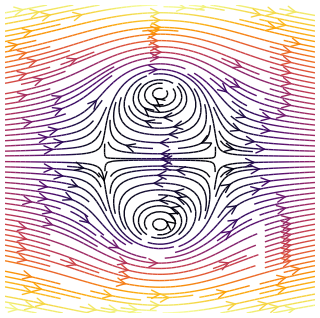
\includegraphics[width=0.3\textwidth,angle=270]{image/Rising_def_Stokes.png}};
        \node (img2) at (0.3\textwidth,0) {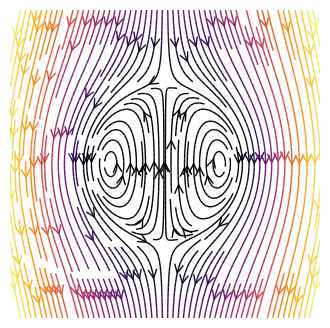
\includegraphics[width=0.3\textwidth]{image/Rising_Stokes.png}};
        % \draw (0.45\textwidth,0)node{$\rightarrow$};
        % \draw (0.45\textwidth,0.4cm)node{$\bm\Gamma_\alpha\cdot \textbf{r}$};
        \node (img1) at (0.0\textwidth,0) {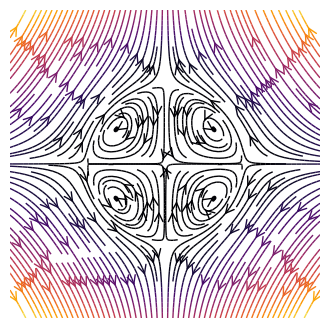
\includegraphics[width=0.3\textwidth]{image/Shear_Stokes.png}};
        \draw (img3.south)node{(c)};
        \draw (img2.south)node{(b)};
        \draw (img1.south)node{(a)};
    \end{tikzpicture}
    \caption{Three examples of steady state flow lines plots of an isolated droplet immersed into a viscous fluid. 
    (a) Rising sphere in uniform stokes flow (analytical solution in \ref{ap:Translating_sphere}). 
    (b) Fixed droplet in extensional flow (analytical solution in \ref{ap:Translating_sphere}).
    (c) Deformed droplet in rising motion (analytical solution of \citet{taylor1964deformation}). }
    \label{fig:flowlines}
\end{figure*}
To summarize, we assume that the inner velocity field of the drop can be decomposed into two distinct part. 
The first one is the steady state component, examples are : hill's vortex for spherical and oblate spheroidal drop in steady linear motion, the inner velocity field of a drop in steady linear flows, and so on. 
The second contribution is the inner velocity fields that alter the drop's shape, this field is assumed linear with the position and homogeneous, that is $\bm\Gamma\cdot \textbf{r}$. 
Adopting these definitions, the particle internal velocity is written, 
\begin{equation}
    \textbf{w}_{2,i}^0(\textbf{x}_\alpha)
    = \bm\Gamma_{\alpha,ik}(t) \cdot \textbf{r}_k
    + \textbf{w}^{s}_{2,i}(t,\textbf{r})
    =\bm{\Omega}_{\alpha,ik}\cdot \textbf{r}_k
    + \textbf{E}_{\alpha,ik} \cdot \textbf{r}_k
    + \textbf{w}^{s}_{2,i}(t,\textbf{r})
    \label{eq:def_vel}
\end{equation}
Where we introduced the vector $\textbf{w}^{s}_2(t,\textbf{r}) =\textbf{w}^{0}_{2,i}(t,\textbf{r})  - \bm\Gamma_{\alpha,ik}(t) \cdot \textbf{r}_k$ which represents all the internal motions that does not alter the drop's shape. 

An important consequence of this definition is that the integral on the RHS of \ref{eq:dt_S_alpha} is null when $\textbf{w}_{2,i}^0 = \textbf{w}_{2,i}^s$. 
This can be shown by re writting the second moment of mass equation with the use of the velocity decomposition.
This yields,
\begin{equation*}
    \ddt \textbf{M}_{\alpha,ik}
    = 
    \textbf{M}_{\alpha,ik} \cdot \bm\Gamma_{\alpha,kj}
    +  \bm\Gamma_{\alpha,ki} \cdot \textbf{M}_{\alpha,jk}
    +
    \intO{ 
        \textbf{w}_{2,i}^s\textbf{r}_j
        + \textbf{r}_i\textbf{w}_{2,j}^s
    }
\end{equation*}
In the cases where $\bm\Gamma = 0$, the droplet shape remains steady, in this case $\ddt \textbf{M}_\alpha = 0$ and $\intO{\textbf{w}^{s}_{2,i} \textbf{r}_j + \textbf{r}_i \textbf{w}_{2,i}^s} = 0$. 
In the case where $\bm\Gamma \neq 0$ the droplets deform according to the linear velocity fields $\bm\Gamma\cdot \textbf{r}$.
Since we assumed that no other source of deformation are present than the latter, we must have $\intO{\textbf{w}^{s}_{2,i} \textbf{r}_j + \textbf{r}_i \textbf{w}_{2,i}^s} = 0$ so that $\textbf{w}^{s}_{2,i} $ doesn't contribute to the deformation nor the rotation.
This, means that $\textbf{w}^{s}_{2,i}$ is a velocity fields determined in  part by the instantaneous shape of the droplet and its , that does not alter the shape of the drop. 
Additionally, the angular momentum is assumed to be entirely described by $\textbf{M}_\alpha \cdot \bm\Omega_\alpha$ meaning that, $\textbf{r} \textbf{w}_{2}^s$ plays no role at all in the total particle's moment of momentum.
This type of velocity fields is encountered in linear skew symmetric flows where the rotation is homogeneous and follow the carrier fluid vorticity. 
Anyhow, this velocity decomposition has the plaisent property that $\textbf{P}_\alpha = \bm\Gamma \cdot \textbf{M}_\alpha + \intO{\textbf{w}^{s}_{2,i} \textbf{r}_j} =  \bm\Gamma \cdot \textbf{M}_\alpha $ at all time, which will simplify the equaitons of motions. 

Now some constrain should apply on the tensor $\textbf{E}_\alpha$.
Indeed, the mass conservation inside the particle \ref{eq:dt_rho} impose $\div \textbf{u}_2^0 = \textbf{E}_\alpha : \textbf{I}= 0$, where it is assumed that $\div \textbf{w}_2^s =0$. 
Also, note that to preserve the spheroidal shape of the particle we must assume that the particle's rate of strain principal direction is the same as the droplet's shape principal axis. 
In other worlds, $\textbf{E}_\alpha$ must have the same eigenbasis as $\textbf{M}_\alpha$. 
Making up with these two constrain leads to the expression : $\textbf{E}_\alpha = -2 E_2 \textbf{pp} + E_2 (\textbf{I}- \textbf{pp})$, where $E_2$ is the second eigenvalue of $\textbf{E}_\alpha$. 


As it is demonstrated in \ref{ap:Translating_sphere} the internal motion of an isolated spherical drop, such as the one in \ref{eq:def_vel}, is entirely determined  from $\textbf{u}_1$,$\grad\textbf{u}_1$,$\textbf{u}_\alpha$ and so on. 
Therefore, it is reasonable to think that in a more general case, $\textbf{w}_2^s$ might be entirely determined by the carrier fluid and particles' properties, namely, $\textbf{u}_\alpha$ $\textbf{M}_\alpha$, $\textbf{u}_1$ $\grad\textbf{u}_1$ and for non-dilute flows we might have $\phi_2$ or more complicated functions. 
Thus, from now on we consider that the internal velocity $\textbf{w}^{s}_2(t,\textbf{r})$ is not part of the particle' unknown, but rather is a closure term. 
Consequently, in this problem a single droplet is described exhaustively by, $\textbf{x}_\alpha, \textbf{u}_\alpha, \textbf{M}_\alpha$ and $\bm\Gamma_\alpha$. 
This requires two additional equations one for $\textbf{M}_\alpha$ and another for $\bm\Gamma_\alpha$. 

\subsubsection*{The conservation equations}

The integrals appearing in \ref{eq:dt_M_alpha} and \ref{eq:dt_P_alpha} can be reformulated using the previous decomposition of the internal velocity field, and it reads, 
\begin{align}
    \intO{(\textbf{rw}_ 2^0 )_{ij}+ (\textbf{w}_2^0 \textbf{r})_{ij}} 
    = \textbf{M}_{\alpha,ik} \cdot \bm\Gamma_{\alpha,jk}
        +  \bm\Gamma_{\alpha,ik} \cdot \textbf{M}_{\alpha,jk}
    \\
    \intO{\rho_2 \textbf{w}_{2,i}^0\textbf{w}_{2,j}^0}
    = \bm\Gamma_{\alpha,jl}\bm\Gamma_{\alpha,ik} \textbf{M}_{\alpha,kl}  
        +\intO{\rho_2 \textbf{w}_{2,i}^s\textbf{w}_{2,j}^s}
    \\
    \intO{\bm\sigma_{2,ij}^0}
    =
    2 \mu_2 v_\alpha \textbf{E}_{\alpha,ij}
    - \intO{p_2^0} \textbf{I}_{ij}
    + \mu_2 \intS{(\textbf{n}_i \textbf{w}_{2,j}^s + \textbf{n}_j \textbf{w}_{2,i}^s)}
    \\
    \intS{\bm\sigma_{I,ij}^0}
    = \frac{\gamma v_\alpha }{a} \left[
        2\textbf{I}_{ij} 
        - \frac{4  }{5} (\textbf{M}_{\alpha,ij}^* - \textbf{I}_{\alpha,ij})
    \right]
    +\mathcal(O)((\textbf{M}_\alpha-\textbf{I})^2)\\
    % s_\alpha 
    % = 4\pi a^2 (1+\frac{\textbf{M}:\textbf{M}}{15})
\end{align}
The reformulation of the moment of momentum have already been treated above. 
The surface tension stress has been derived in the limit of small deformation. 
Note that our formula agree with the one derived by \citet{lhuillier1987phenomenology}. 
The detailed calculation of the surface tension stress tensor is given in appendix. 
We provide the exact results as well as the Taylor expansion of this formula for small deformation. 

Injecting these formulas inside \ref{eq:dt_M_alpha} and \ref{eq:dt_P_alpha} yields an equation for the deformation and the rate of strain of the drop. 
If we separate the skew-symmetric, symmetric and trace of the moment of momentum equation we obtain and equation for $\bm\Omega_\alpha$ and one fer  $\textbf E_\alpha$, namely,
\begin{align*}
    % \ddt \textbf{pp}_{\alpha,ij}
    % = \textbf{pp}_{\alpha,ik} \cdot \bm\Omega_{\alpha,jk}
    % +  \bm\Omega_{\alpha,ik} \cdot \textbf{pp}_{\alpha,jk}\\
    \ddt \textbf{M}_{\alpha,ij}
    = \textbf{M}_{\alpha,ik} \cdot \bm\Gamma_{\alpha,jk}
    +  \bm\Gamma_{\alpha,ik} \cdot \textbf{M}_{\alpha,jk}\\
    \ddt (\textbf{I}_{\alpha,ik}\bm\omega_{\alpha,k} )
    = 
    \intS{(\textbf{r}\times\bm\sigma_1^0\cdot \textbf{n})_i} \\
    \frac{1}{2}\ddt^2 \textbf{M}_{\alpha,ij}
    -  \bm\Gamma_{\alpha,jl}\bm\Gamma_{\alpha,ik} \textbf{M}_{\alpha,kl}  
    + \mu_2 v_\alpha 2\textbf{E}_{\alpha,ij}
    + \frac{\gamma v_\alpha }{a} \left[
    2\textbf{I}_{ij} 
    - \frac{4 }{5} (\textbf{M}_{\alpha,ij}^* - \textbf{I}_{\alpha,ij})
    \right]\\
    = 
    \frac{1}{2}\intS{(\textbf{r}\bm\sigma_1^0 + \bm\sigma_1^0\textbf{r})\cdot \textbf{n}} 
    + \intO{\rho_2 \textbf{w}_{2,i}^s\textbf{w}_{2,j}^s}
    + \intO{p_2^0} \textbf{I}_{ij}
    - \mu_2 \intS{(\textbf{n}_i \textbf{w}_{2,j}^s + \textbf{n}_j \textbf{w}_{2,i}^s)}\\
    % \frac{1}{2}\ddt^2 \textbf{M}_{\alpha,mm}
    % -  \bm\Gamma_{\alpha,ml}\bm\Gamma_{\alpha,mk} \textbf{M}_{\alpha,kl}  
    % + \frac{\gamma v_\alpha }{a} 
    % \left[
    % 2\textbf{I}_{mm} 
    % % - \frac{4 }{5 } (\textbf{M}_{\alpha,mm}^* - \textbf{I}_{\alpha,mm})
    % \right]
    % = 
    % \intS{\textbf{r}_m\cdot\bm\sigma_{1,mk}^0\cdot \textbf{n}_k} 
    % + \intO{\rho_2 \textbf{w}_{2,m}^s\cdot \textbf{w}_{2,m}^s}
    % + \intO{p_2^0} \textbf{I}_{mm}
\end{align*}
The second moment of mass \ref{eq:dt_Cs}, is consistent with the equation found by \citet{goddard1967nonlinear} and \citet{lhuillier1987phenomenology}. 
Following, \citet{goddard1967nonlinear}  terminology, the left-hand side of \ref{eq:dt_Cs} is referred as the \textit{convected} derivative of $\textbf{M}^*_\alpha$. 
Therefore, the \textit{convected} derivative of $\textbf{M}_\alpha$ is equal to the rate of strain of the particle. 
The skew-symmetric part of the first moment of momentum \ref{eq:dt2_C}, it is basically the angular momentum balance of a non-spherical object. 
The right-hands side accounting for the external torque contribution. 
The symmetric part however has the form of a non-linear forced harmonic oscillatory equation for the droplet deformation. 
Indeed, the first groups of terms on the left-hand side represent the inertial contribution of the droplet internal fluid. 
It is made of a second order derivative plus non-linear terms in $\bm\Gamma_\alpha$. 
The second groups of terms is internal viscous contribution that arise directly from the definition of the stress \ref{eq:sigma_2_def}. 
It vanishes for small viscosity ration and is linear in the first derivative of $\textbf{M}_\alpha$. 
The last term on the left-hand side is the elastic response from the interface which is negligible for high capillary number $Ca \to \infty$. 
Then on right-hand side of the equation we find the first moment of surface force, $\intS{(\textbf{r}\bm\sigma_1^0+ \bm\sigma_1^0\textbf{r})\cdot \textbf{n}}^*$ which has an unknown expression at this stage. 
\ref{eq:dt2_C} might be regarded as a second order harmonic equation with non-linear contributions. 
However, the unknown integrals $\intO{\rho_2 \textbf{w}_{2,i}^s\textbf{w}_{2,j}^s},
\intS{(\textbf{n}_i \textbf{w}_{2,j}^s + \textbf{n}_j \textbf{w}_{2,i}^s)}$ and $\intS{(\textbf{r}\bm\sigma_1^0+ \bm\sigma_1^0\textbf{r})\cdot \textbf{n}}^*$ are in general function of the shape of the particle so on $\textbf{M}_\alpha$ and its higher derivatives of $\textbf{M}_\alpha$.
These terms have to be seen as forcing terms. 
Therefore, at this stage it is impossible to predict the nature of the harmonic regime followed by the droplet. 
To conclude on this matter one must find an expression for all this closure as well as determinate the impact of the non-linear terms.



We now focus on the rate of strain equation. 
To better understand this equation we introduce the following dimensionless groups, 
\begin{align*}
    \intO{\rho_2 \textbf{w}_{2,i}^0\textbf{w}_{2,j}^0}
    \sim \frac{m_\alpha a^2}{\tau_u^2} \textbf{F}_{ww}^*
    \\
    - \intO{p_2^0\textbf{I}}
    + \mu_2 \intS{(\textbf{n}_i \textbf{w}_{2,j}^s + \textbf{n}_j \textbf{w}_{2,i}^s)}
    \sim \frac{v_\alpha \mu_2}{\tau_u} \textbf{F}_{e}^*
    \\
    \intS{\textbf r \bm\sigma_1^0 \cdot \textbf{n}}
    \sim 
    \frac{v_\alpha \mu_1}{\tau_u} \textbf{F}_{\sigma}^*
\end{align*} 
where we have assumed that the internal and external stress contribution followed a viscous scaling. 
The time $\tau_u$ represent the external solicitation time-scale. 
Which is in opposition to the droplets rate of strain and rotation time scale such that $\bm\Gamma = 1/\tau \bm\Gamma^*$. 
\begin{align*}
    \frac{\zeta Re}{5}\left[
        \beta^2 \frac{1}{2}\ddt^2 \textbf{M}_{\alpha,ij}
    -   \beta^2 \bm\Gamma_{\alpha,jl}\bm\Gamma_{\alpha,ik} \textbf{M}_{\alpha,kl}  
    - \textbf{F}_{ww}^*
    \right]
    + \lambda  \left[
        \beta 2\textbf{E}_{\alpha,ij}
    +  \textbf{F}_\sigma^*
    \right]
    + \frac{1}{Ca} \left[
    2\textbf{I}_{ij} 
    - \frac{4  }{5} (\textbf{M}_{\alpha,ij}^* - \textbf{I}_{\alpha,ij})
    \right]
    = 
    \frac{1}{2}
    \textbf{F}_{\sigma_1}^*
    % \intS{(\textbf{r}\bm\sigma_1^0 + \bm\sigma_1^0\textbf{r})\cdot \textbf{n}} 
    % + \intO{p_2^0} \textbf{I}_{ij}
\end{align*}
where we have defined the following dimensionless groups : 
\begin{align*}
    \beta = \frac{\tau_u}{\tau}
    && \zeta = \rho_2 /\rho_1
    && \lambda = \mu_1/\mu_2 
    && Re = \frac{\rho_1 a^2 }{ \mu_1 \tau_u}
    && Ca = \frac{a \mu_1}{\gamma \tau_u}
\end{align*}

We now examine the specific case studied by \citet{lamb1924hydrodynamics} where he considered no external contribution around the particle nor rotational motion.
Also, it is considered that the deformation within the particle are linear and small. 
Keeping only the trace of this equation yields the low deformation system of equation :
\begin{align*}
    \ddt \textbf{M}_{\alpha,ij} = \textbf{E}_{\alpha,ij}\\
    \frac{\zeta Re}{5}
        \beta^2 \frac{1}{2}\ddt^2 \textbf{M}_{\alpha,ij}
    % -   \beta^2 \bm\Gamma_{\alpha,jl}\bm\Gamma_{\alpha,ik} \textbf{M}_{\alpha,kl}  
    % - \textbf{F}_{ww}^*
    % \right]
    + \lambda 
        \beta 2\textbf{E}_{\alpha,ij}
    % +  \textbf{F}_\sigma^*
    % \right]
    - \frac{1}{Ca} 
     \frac{4  }{5} (\textbf{M}_{\alpha,ij}^* - \textbf{I}_{\alpha,ij})
    = 0
    % \frac{1}{2}
    % \textbf{F}_{\sigma_1}^*
    % \intS{(\textbf{r}\bm\sigma_1^0 + \bm\sigma_1^0\textbf{r})\cdot \textbf{n}} 
    % + \intO{p_2^0} \textbf{I}_{ij}
\end{align*}
Notice that this is a second order oscillatory equation. 
This is equivalent to  \citet{lamb1924hydrodynamics}. 
Therefore our model is somewhat more general. 

Lastly, as it will be usefull for latter let consider the cases wheer the timescale of the flow is much smaller that the one of the particle rate of strain, in this case $\beta \ll 1$. 
Making use of this fact makes the moment of momentum equation as, 
\begin{align*}
    - \frac{\zeta Re}{5}
     \textbf{F}_{ww}^*
    + \lambda  
    \textbf{F}_\sigma^*
    + \frac{1}{Ca} \left[
    2\textbf{I}_{ij} 
    + \frac{4  }{5} (\textbf{M}_{\alpha,ij}^* - \textbf{I}_{\alpha,ij})
    \right]
    = 
    \frac{1}{2}
    \textbf{F}_{\sigma_1}^*
    % \intS{(\textbf{r}\bm\sigma_1^0 + \bm\sigma_1^0\textbf{r})\cdot \textbf{n}} 
    % + \intO{p_2^0} \textbf{I}_{ij}
\end{align*}
This is the steady state equilibrium equation of the first moment of force. 
If the capillary number is low enough the last term  completely balance the external stress. 

Two distinct descriptions can be applied to the dispersed phase, while only one description is applicable to the fluid phase. 
In this section, we derive averaged equations for the dispersed phase using Lagrangian conservation laws. 
Following this, we  discuss the equivalence between the particle or lagrangian averaged equations for the dispersed phase and the averaged equations for the dispersed phase presented in \ref{sec:two-fluid}.


%Two different descriptions are possible for the dispersed phase while one is available for the fluid phase. 
%In this part we first derive averaged equations for the dispersed phase based on Lagrangian conservation laws. 
%Then we provide a complete discussion regarding the equivalence between the "lagrangian" averaged equations for the dispersed phase and the averaged equations governing the dispersed phase presented in \ref{sec:two-fluid}. 
%based on 
%the set of equations just derived and the averaged equations governing the dispersed phase presented in \ref{sec:two-fluid}. 

\subsection{Dispersed phase averaged equations}

In the preceding section, we have described the dispersed phase using a Lagrangian framework. 
However, to ensure consistency with the Eulerian conservation equations that describe the continuous phase, it is necessary to extend the Lagrangian equations to an Eulerian description. 
The approach presented here follows the methodology pioneered by \citep{lhuillier1992ensemble}.
%In the last section, we have described the dispersed phase within a Lagrangian framework.
%However, to be consistent with the Eulerian conservation equations used to describe the continuous phase, we need to extend the Lagrangian equations to an Eulerian description. 
%The strategy exposed here follow the approach pionnered by \citep{lhuillier1992ensemble}.
%In order to achieve this,
We introduce the function $\delta_\alpha$, which is defined as follows, 
\begin{align}
    \delta_\alpha(\textbf{x},\textbf{x}_\alpha(t,\FF)) 
    = \delta(\textbf{x}-\textbf{x}_\alpha(t,\FF)),
    \label{eq:delta_alpha}
\end{align}
where $\delta$ is the Dirac function.
Note that we explicitly note the arguments $(t,\FF)$ to highlight that the position of the particle $\alpha$ is a function of time and of the flow configuration $\FF$.
Applying the chain rule yields \citep{lhuillier1998}%we may write the partial time derivative of $\delta_\alpha$ can be written as
%\begin{equation}
%\frac{\partial \delta_\alpha(\textbf{x},\textbf{x}_\alpha(t,\FF))}{\partial t} 
%=  \frac{\partial \textbf{x}_\alpha}{\partial t} 
%\cdot \frac{\partial \delta_\alpha}{\partial \textbf{x}_\alpha}(\textbf{x},\textbf{x}_\alpha(t,\FF)) .
%\end{equation}
%This leads to the following expression, 
\begin{equation}
    \pddt \delta_\alpha
    + \div (\textbf{u}_\alpha  \delta_\alpha)
    =0,
    \label{eq:dt_delta_alpha}
\end{equation}
where we used the identity, $\frac{\partial \delta_\alpha}{\partial \textbf{x}_\alpha}  = -\grad \delta_\alpha$ and the fact that $\textbf{u}_\alpha(t,\FF)$ is not a function of $\textbf{x}$. 
\ref{eq:dt_delta_alpha} does not apply in scenarios where topological changes occur, such as break-up or coalescence events. 
In these cases, a source term can be introduced on the right-hand side of \ref{eq:dt_delta_alpha}, similar to the approach used in population balance equations, to account for the birth or death of particles \citep{randolph2012theory}.
%It should be noted that \ref{eq:dt_delta_alpha} is not applicable if changes in topology, such as break-up or coalescence events, occur.
%In such cases it is possible, as it is done in population balance equations, to include a source term on the RHS of \ref{eq:dt_delta_alpha} to account for particle birth or death. 
%Multiplying each Lagrangian quantities $\text q_\alpha$ by $\delta_\alpha$ yields the field $\text q_\alpha(t,\FF)\delta_\alpha(\textbf{x},t,\FF)$, which is defined over the entire domain $\Omega$.
%Likewise, for any derivative of Lagrangian quantities, such as $\ddt \text q_\alpha$, we define its corresponding Eulerian field by multiplying $\ddt \text q_\alpha$ with $\delta_\alpha$ and show that :
By multiplying each Lagrangian quantity $\text q_\alpha$​ by $\delta_\alpha$​, we obtain the field $\text q_\alpha(t,\FF)\delta_\alpha(\textbf{x},t,\FF)$, which is defined throughout the entire domain $\Omega$. 
Similarly, for any derivative of a Lagrangian quantity, such as $\ddt \text q_\alpha$​, the corresponding Eulerian field is defined by multiplying $\ddt \text q_\alpha$ with $\delta_\alpha$ 
%This can be expressed as
Given that $\text q_\alpha(t,\FF)$ and $\textbf{u}_\alpha(t,\FF)$ do not depend on \textbf{x}, and by using Equation \ref{eq:dt_delta_alpha}, we obtain
\begin{equation}
    \delta_\alpha \ddt \text q_\alpha
    = \pddt (\delta_\alpha \text q_\alpha)
    + \div (\delta_\alpha \text q_\alpha \textbf{u}_\alpha).
    \label{eq:dt_delta_alpha_q_alpha}
\end{equation}
%where we have used the fact that $\text q_\alpha(t,\FF)$ and $\textbf{u}_\alpha(t,\FF)$ are not function of \textbf{x}, and we made use of \ref{eq:dt_delta_alpha}.
%Now let us consider a domain containing $N$ particles.
%We define what we call the \textit{particle field} of a quantity $\text q_\alpha$, as the sum of the $\delta_\alpha \text q_\alpha$ over all particles in the flow, namely $\displaystyle\sum_{\alpha=0}^N \delta_\alpha \text q_\alpha$.
%Notice that \ref{eq:dt_delta_alpha_q_alpha} remains valid for a sum of fields since derivative and sum operators commute.
Consider a domain containing $N$ particles. We define the \textit{particle field} for a quantity $\text q_\alpha$​ as the sum of $\delta_\alpha \text q_\alpha$ over all particles within the domain, expressed by $\displaystyle\sum_{\alpha=0}^N \delta_\alpha \text q_\alpha$​. 
Note that the formula given by \ref{eq:dt_delta_alpha_q_alpha} remains valid for the sum of such fields, since the operations of differentiation and summation commute.
%In the objective of obtaining averaged equations for the dispersed phase, we introduce the average of $\text q_\alpha$ as  
To obtain the averaged equations for the dispersed phase, we define the particle average of $\text q_\alpha$​ as
\begin{equation}
     n_p \text q_p(\textbf{x},t) = \avg{\sum_\alpha\delta_\alpha \text q_\alpha},
     \label{eq:p_avg}
\end{equation}
where, $n_p(\textbf{x},t) = \avg{\sum_\alpha \delta_\alpha}$ is the probability density of finding a particle center of mass in the infinitesimal volume $d\textbf{x}$ around \textbf{x}, and $\text q_p(\textbf{x},t)$ is the average of $\text q_\alpha$ conditionally on the presence of a particle at \textbf{x} and time $t$. 
To simplify the notations, we consider the shorthand \citep{lhuillier1998},
\begin{equation*}
    \sum_\alpha \delta_\alpha \to \delta_p, 
\end{equation*}
such that $\pavg{\text q_\alpha}=\avg{\sum_\alpha \delta_\alpha \text q_\alpha}=n_p\text q_p$.
Note that we used the subscript $_p$ on $\text q_p$ to denote that this represents a particle-averaged field, initially derived from Lagrangian quantities. 
%Furthermore, in view of equation   
Additionally, in light of \ref{eq:def_fluctu} we define the fluctuating part of a particle field $\text q_p$ as
\begin{equation}
    \text q_\alpha' = \text q_\alpha - \text q_p. 
    \label{eq:def_fluc_p}
\end{equation}

To obtain the particle phase averaged equations one multiply \ref{eq:dt_q_alpha_tot} and \ref{eq:dt_Q_alpha_tot} by $\delta_\alpha$ and apply the ensemble average (\ref{eq:avg}), this yields
\begin{align}
    \pddt (n_p\text Q_p)
    + \div (n_p \text Q_p \textbf{u}_p + \pavg{\textbf{u}_\alpha' \text Q_\alpha'})
    = \pOavg{ s_d^0 }
    + \pSavg{ s_I^0 }\nonumber\\
    + \pSavg{ \left[\mathbf{\Phi}_f^0 + f_f^0 (\textbf{u}_\Gamma^0-\textbf{u}_f^0) \right] \cdot \textbf{n}_d },
    \label{eq:avg_dt_dq_alpha_tot}\\
    \pddt (n_p\textbf{Q}_p^{(1)})
    + \div \left(n_p \textbf{Q}_p^{(1)} \textbf{u}_p + \pavg{\textbf{u}_\alpha' \textbf{Q}_\alpha^{(1)'}}\right)
    =\pOavg{ \left(
        \textbf{r} s_d^0         
        + f_d^0  \textbf{w}_d^0 
        - \mathbf{\Phi}_d^0
    \right) }\nonumber\\
    + \pSavg{ \left(
        \textbf{r}s_\Gamma^0
        + f_\Gamma^0 \textbf{w}_\Gamma^0
        - \mathbf{\Phi}_{\Gamma||}^0
    \right) }
    + \pSavg{ \textbf{r} \left[
        \mathbf{\Phi}_f^0
        + f_f^0 (\textbf{u}_\Gamma^0-\textbf{u}_f^0)
    \right]\cdot \textbf{n}_d  }.
    \label{eq:avg_dt_dQ_alpha_tot}
\end{align}
The derivation of the higher moment particle-averaged equations is provided in \ref{ap:Moments_equations}.
The only fluxes appearing in \ref{eq:avg_dt_dq_alpha_tot} and \ref{eq:avg_dt_dQ_alpha_tot} are the fluctuation tensors $\pavg{\textbf{u}_\alpha' \text q_\alpha'}$ and $\pavg{\textbf{u}_\alpha' \textbf{Q}_\alpha'}$. 
Therefore, the non-convective fluxes $\bm\Phi_d^0$ and $\bm\Phi_I^0$ do not play the role of macroscopic fluxes, as it is the case in \ref{eq:avg_dt_chi_f} and \ref{eq:avg_dt_delta_f}. Instead, they act as source terms in the first moment and higher moment equations. 
This distinction is the main structural differences between the Kinetic-like model (\ref{eq:avg_dt_dq_alpha_tot} and \ref{eq:avg_dt_dQ_alpha_tot}) and the two-phase flow model (\ref{eq:avg_dt_chi_f} and \ref{eq:avg_dt_delta_f}). 
In this study, \ref{eq:avg_dt_chi_f} and \ref{eq:avg_dt_delta_f} are referred to as the phase-averaged equations, while \ref{eq:avg_dt_dq_alpha_tot} and \ref{eq:avg_dt_dQ_alpha_tot} are called the particle-averaged equations. 


 





\section{The hybrid model}
\label{sec:averaged_eq}
% \subsection{Phase average and particle averaged equations}
% Correspondingly, we take the average of the particle fields equations by using \ref{eq:avg} on \ref{eq:dt_dq_alpha_tot} and \ref{eq:dt_dQ_alpha_tot}, which gives, 
In the objective of obtaining coarse-grained level equations for the dispersed phase, one must apply an ensemble average operator on \ref{eq:avg_dt_dq_alpha_tot} and \ref{eq:avg_dt_dQ_alpha_tot} which is made possible since the particle fields $\delta_\alpha \ldots$ are now defined over the whole space $\Omega$ thanks to the Dirac delta functions $\delta_\alpha$.  
These equations yields,
\begin{align}
    \pddt \avg{\delta_\alpha  q_\alpha^\text{tot}}
    + \div \avg{\delta_\alpha\textbf{u}_\alpha q_\alpha^\text{tot}}
    &= \pOavg{ s_2^0 }
    + \pSavg{ s_I^0 }
    + \pSavg{ \left[\mathbf{\Phi}_1^0 + f_1^0 (\textbf{u}_I^0-\textbf{u}_1^0) \right] \cdot \textbf{n}_2 ,}
    \label{eq:avg_dt_dq_alpha_tot}\\
    \pddt \avg{\delta_\alpha \mathcal{Q}_\alpha^\text{tot}}
    + \div \avg{\delta_\alpha\textbf{u}_\alpha\mathcal{Q}_\alpha^\text{tot}}
    &=\pOavg{ \left(
        \textbf{r} s_2^0         
        + f_2^0  \textbf{w}_2^0 
        - \mathbf{\Phi}_2^0
    \right) }
    + \pSavg{ \left(
        \textbf{r}s_I^0
        + f_I^0 \textbf{w}_I^0
        - \mathbf{\Phi}_{I||}^0
    \right) }\nonumber\\
    &+ \pSavg{ \textbf{r} \left[
        \mathbf{\Phi}_1^0
        + f_1^0 (\textbf{u}_I^0-\textbf{u}_1^0)
    \right]\cdot \textbf{n}_2  }.
    \label{eq:avg_dt_dQ_alpha_tot}
\end{align}
In \ref{ap:Moments_equations} the derivation of the higher moment particle-averaged equations is provided. 
In this study,\ref{eq:avg_dt_chi_f} and \ref{eq:avg_dt_delta_f} are refereed to as the phase-averaged equations, while \ref{eq:avg_dt_dq_alpha_tot} and \ref{eq:avg_dt_dQ_alpha_tot} are denoted as the particle-averaged equation. 
In these expressions we kept a general notation yet. 
But note that, we can note the particle phase averaged quantity by,
\begin{equation}
     n_p q_p(\textbf{x},t) = \avg{\delta_\alpha q_\alpha}
     \label{eq:p_avg}
\end{equation}
where, $n_p(\textbf{x},t) = \avg{\delta_\alpha}$ is the probable number of finding a particle center of mass at $\textbf{x}$
and $q_p$ is the conditional average of $q_\alpha$ conditionally on the presence of a particle at \textbf{x}. 
Additionally, notice that it is possible to define the fluctuating parts of a property by, 
\begin{equation}
    q_\alpha' = q_\alpha - q_p
    % \;\;\;\;\;\;\text{and}
    % \;\;\;\;\;\;
\end{equation}
such that the particle average of a product can be rewritten, $\pavg{q_\alpha\textbf{u}_\alpha} = n_p q_p \textbf{u}_p + \pavg{q_\alpha' \textbf{u}_\alpha'}$. 
These notations will find their use in \ref{sec:averaged_eq}, but for now we keep the formulation rather generic as in \ref{eq:avg_dt_dQ_alpha_tot} and \ref{eq:avg_dt_dq_alpha_tot}

As remarked by \citet{jackson1997locally} for the angular momentum equations of solid spherical particles, and here in a more general case :\ref{eq:avg_dt_chi_f} and \ref{eq:avg_dt_dq_alpha_tot} may seem to be not coupled with the higher order moments equations, i.e. \ref{eq:avg_dt_dQ_alpha_tot}. 
Indeed, the first order moment $\mathcal{Q}_p^\text{tot}$ do not appear explicitly in either \ref{eq:avg_dt_chi_f} or \ref{eq:avg_dt_dq_alpha_tot}.
However, the exchange and source terms 
appearing in both \ref{eq:avg_dt_chi_f} and \ref{eq:avg_dt_dQ_alpha_tot} might depend on the higher order moments of the particles.
Indeed, in the momentum equation of the continuous phase, i.e. the ensemble average of \ref{eq:dt_rhou_k}, the exchange term corresponds to the averaged drag force, namely $\pSavg{\bm{\sigma}_1^0\cdot \textbf{n}_2}$. 
It is clear that $\pSavg{\bm{\sigma}_1^0\cdot \textbf{n}_2}$ has a strong dependency with $\textbf{u}_p$,$\mathcal{P}_p$ and $\mathcal{M}_p$ since the drag force is a function of both the particle's kinematic and its shape. 
Therefore, \ref{eq:avg_dt_dQ_alpha_tot} is linked to \ref{eq:avg_dt_chi_f} and \ref{eq:avg_dt_dq_alpha_tot} solely through the dependence of the exchange and source terms with the properties of the particles, e.g. $q_p,\mathcal{Q}_p$ and possibly the higher order moments. 
This reasoning applies for the energy equation and all kinds of conservation equation. 
Ultimately, the significance of the higher moments equations can be evaluated based on the dependency of the closure terms present in \ref{eq:avg_dt_chi_f} with the properties of the particle : $q_p, \mathcal{Q}_p$ and potentially the higher-order moments of the particles. 



%\subsubsection*{Equivalence between particle and continuous models}
\subsection{Equivalence between particle-averaged and phase-averaged equations}
\label{sec:equivalence}
%To model the dispersed phase we can either use \ref{eq:avg_dt_chi_f} with $k=d$, or the particle-averaged equations: \ref{eq:avg_dt_dq_alpha_tot}, \ref{eq:avg_dt_dQ_alpha_tot} and possibly the higher moments equations in \ref{ap:Moments_equations}. 
%Consequently, it is fair to address the question of the compatibility and differences between both formalisms. 
To model the dispersed phase, there are two distinct approaches. 
We can either use \ref{eq:avg_dt_chi_f} with $k=d$, or we can employ the particle-averaged equations \ref{eq:avg_dt_dq_alpha_tot}, \ref{eq:avg_dt_dQ_alpha_tot} and potentially the higher moments equations found in \ref{ap:Moments_equations}.
Consequently, it is important to address the compatibility between these two formalisms.
It has been demonstrated in various studies \citep{buyevich1979flow,lhuillier1992ensemble,jackson1997locally,zhang1994averaged}, that phase-averaged quantities can be expressed as a Taylor series expansion of particle-averaged quantities. 

The aforementioned studies used the single-particle conditionally averaged approach to demonstrate this equivalence.  
In this work we use instead the ``distributional'' approach of \citet{pahtz2023general} since, as shown below it yields more general and simpler formulation. 
The dispersed phase indicator function $\chi_d$ can be expressed as a sum of phase indicator function, $\chi_d(\textbf{x},t,\FF) = \sum_\alpha\chi_\alpha(\textbf{x},t,\FF)$ where $\chi_\alpha =1$ in the particle domain $\Omega_\alpha(\FF,t)$ and $0$ otherwise. 
Thus, any dispersed phase quantity pertaining to a single particle can be written as, 
\begin{equation}
   f^0_d \chi_\alpha(\textbf{x},t,\FF)
   = 
   \int_{\mathbb{R}^3} 
    f^0_d \chi_\alpha(\textbf{x}_\alpha + \textbf{r},t,\FF)\delta(\textbf{x} - \textbf{x}_\alpha - \textbf{r}) 
    d\textbf{r} 
   \label{eq:taylor_f_d}
\end{equation}
Likewise, we assume that the interface indicator function $\delta_\Gamma$ can be partitioned into $N$ interface indicator function such that $\delta_\Gamma =  \sum_\alpha  \delta_{\Gamma\alpha}$.
In that case any surface-averaged quantities may be written, 
\begin{equation}
    f_\Gamma^0 \delta_\Gamma(\textbf{x},t,\FF) = 
    \sum_\alpha 
    \int_{\mathbb{R}^3} 
     f_\Gamma^0 \delta_{\Gamma\alpha}(\textbf{x}_\alpha + \textbf{r},t,\FF)\delta(\textbf{x} - \textbf{x}_\alpha - \textbf{r}) 
     d\textbf{r}. 
    \label{eq:taylor_f_I}
\end{equation}
% Notice that \ref{eq:taylor_f_d} and \ref{eq:taylor_f_I} are well-defined in the distributional sense since the integral on the right-hand side of both equations correspond to a convolution product.
Notice that the integral on the right-hand side of \ref{eq:taylor_f_d} and \ref{eq:taylor_f_I} correspond to a convolution product.
Additionally, since the Dirac distribution $\delta(\textbf{x} - \textbf{x}_\alpha - \textbf{r})$, is the unit of convolution \ref{eq:taylor_f_d} is verified (see \citet[Chapter 9]{appel2007}).
The convolution product of the Dirac delta and the derivative of the Heaviside distribution is also well-defined, see \citet[Chapter 9]{appel2007}.
It follows that \ref{eq:taylor_f_d} and \ref{eq:taylor_f_I} are well-defined in the distributional sense. 
Upon using the Taylor expansion of the Dirac delta function $\delta(\textbf{x} - \textbf{x}_\alpha - \textbf{r})$ in the neighborhood of $\textbf{r}=0$ one obtain,
\begin{equation}
\delta(\textbf{x} - \textbf{x}_\alpha - \textbf{r})
= \delta(\textbf{x} - \textbf{x}_\alpha)
- \textbf{r}\cdot\grad \delta(\textbf{x} - \textbf{x}_\alpha)
+ \frac{\textbf{rr}}{2}:\grad\grad\delta(\textbf{x} - \textbf{x}_\alpha) 
- \ldots.
% + \ldots
\label{eq:exp_delta}
\end{equation}
Injecting \ref{eq:exp_delta} into \ref{eq:taylor_f_d} and \ref{eq:taylor_f_I}, and noticing that the indicator functions, $\chi_\alpha$ and $\delta_\Gamma$, reduce the domain of integration from $\mathbb{R}^3$ to, $\Omega_\alpha$ and $\Gamma_\alpha$, respectively,  yields: 
\begin{align}
    f^0_d \chi_d
    =\delta_p\intO{f^0_d}
    - \div\left(\delta_p\intO{\textbf{r} f^0_d}\right)
    + \frac{1}{2}\grad\grad :\left(\delta_p\intO{\textbf{rr} f^0_d}\right)
    \ldots 
    \label{eq:fd_asympt}
   \\
   f_\Gamma^0 \delta_\Gamma 
   =\delta_p\intS{f^0_\Gamma}
   - \div\left(\delta_p\intS{\textbf{r} f^0_\Gamma}\right)
   + \frac{1}{2}\grad\grad :\left(\delta_p\intS{\textbf{rr} f^0_\Gamma}\right)
   \ldots 
   \label{eq:fG_asympt}
%    \\
\end{align} 
Where we recognize the zeroth, first and second order moments of $f_d^0$ and $f_\Gamma^0$, into \ref{eq:fd_asympt} and \ref{eq:fG_asympt}, respectively. 
Notice that even before applying any kind of averaging procedure \ref{eq:fd_asympt} and \ref{eq:fG_asympt} illustrates the connection between the dispersed phase fields, of the form $\chi_d(\ldots)$ or $\delta_\Gamma(\ldots)$, and the particle fields of the form $\delta_p(\ldots)$. 
It is interesting to notice that these relations hold in a distributional sense at a local level. 


Applying similar considerations to the interface indicator function $\delta_\Gamma$, and averaging over all configurations, we obtain the general relations that link continuous-averaged and particle-averaged fields, namely \citep{lhuillier1992ensemble,lhuillier1998,lhuillier2000bilan}, 
\begin{align}
    \avg{\chi_df_d^0} 
    &=  \pavg{\text q_\alpha}
        - \div  
        \pavg{\textbf{q}_\alpha^{(1)}}        
        + \frac{1}{2} \grad\grad : \pavg{\textbf{q}_{\alpha}^{(2)}}
        + \ldots  \label{eq:f_exp_chi} \\
    \avg{\delta_\Gamma  f_\Gamma ^0} 
    &=  \pavg{\text q_{\Gamma \alpha}}        
        - \div \pavg{\textbf{q}_{\Gamma\alpha}^{(1)}}
        + \frac{1}{2} \grad\grad : \pavg{\textbf{q}_{\Gamma\alpha}^{(2)}}
        + \ldots  
    \label{eq:f_exp_delta}
\end{align}
%\JL{j'ai ajoute la sommes des contributions dans les particules et de surfaces}
Summing \ref{eq:f_exp_chi} and \ref{eq:f_exp_delta} we obtain
\begin{equation}
    \avg{\chi_df_d^0+\delta_\Gamma  f_\Gamma ^0} = \pavg{\text Q_\alpha}
    - \div  
    \pavg{\textbf{Q}_\alpha^{(1)}}        
    + \frac{1}{2} \grad\grad : \pavg{\textbf{Q}_{\alpha}^{(2)}}
    + \ldots  \label{eq:f_exp}
\end{equation}
When considering an infinite number of terms in \ref{eq:f_exp} one might eventually obtain a converged approximation of $\avg{\chi_d f_d^0+\delta_\Gamma  f_\Gamma ^0}$. 
However, it is important to note that Taylor series have what is known as a \textit{radius of convergence} beyond which adding more terms does not necessarily improve the approximation \citep[Chapter 1]{appel2007}. 
In particular, for distances beyond a certain limit \textbf{r} the series might diverges depending on the behavior of the function $\avg{\chi_d f_d^0+\delta_\Gamma  f_\Gamma ^0}$ near the point $\textbf{x}$. 
For the purposes of this article, we will assume that the Taylor series has an infinite radius of convergence, although this assumption warrants further investigation.%function $f_d^0$ evaluated at a point $\textbf{x}_\alpha$ is greater than the particle size, then \ref{eq:f_exp} might converges and provides a good approximation.
%\JL{j'ai vraiment raccourci cette partie, car meme si je la trouve pertinente il y a des elements que je trouvais peu claire:
%\begin{itemize}
%\item tu dis que "to assume that $f_d$ is slowly variying at the scale of the particle", justement je ne pense pas que l'on veuille cela car sinon a quoi serve les moments d'ordres superieurs.
%Par ailleurs pr moi (mais peut etre que je me trompe), le rayon de convergence dsun' serie de Taylor n'a rien a voir avec le fait que la fonction dont on cherche la serie varie peu à l'endroit du developpement
%Enfin sur cette idée de precision de la série, pr moi le developpement en série se fait dans l'hypothèse ou la grandeur d'interet (moyennée) varie peut sur l'échelle des grandeurs macroscopiques
%en gros un developpement limite en $a/L$ ou $L$ est la taille des echelles macro.
%\end{itemize}
%}

%In brief, high care must be taken when using these kind of taylor expansion especially in that context since we do not know the exact form of $f_d$.  
%Nevertheless it is reasonable to assume that $f_d$ is slowly variying at the scale of the particle with a radius of convergence sufficiently large, in this case \ref{eq:f_exp} might provide a good approximation, 
%and we might expect an error of $\mathcal{O}[(a/L)^{n}]$ when the highest moment of the series is of order $n-1$ with $L$ being a macroscopic length scale. 
%It is within the context of this assumption that the following disscussion takes place. 

% \JL{pour l'instant j'ai eneleve la partie applicative (meme si elle me semble tres interessante). 
% D'ailleurs pq le second terme du dvt pr les conservation de la masse est nul ? 
% Ce serait bien de donner de petites lois d'echelles pr evaluer les ordres de grandeurs de chacun des termes.}
%Particularly we note that if $f_d^0 = \rho_d$ and $f_d^0 = \rho_d \textbf{u}_d^0$ we obtain, 
%\begin{align}
%    \label{eq:f_exp_exe1}
%    \phi_d \rho_d
%    = m_p n_p 
%    + \frac{1}{2}\grad^2 : (n_p\textbf{M}_p)+\ldots,\\
%    \phi_d \rho_d \textbf{u}_d
%    = m_p n_p \textbf{u}_p 
%    - \div (n_p\textbf{P}_p)+\ldots,
%    \label{eq:f_exp_exe}
%\end{align}
%respectively. 
%Meaning that $\phi_d\rho_d$ is related to the shape of the particles, represented by $\textbf{M}_p$ through \ref{eq:f_exp_exe1}.
%Additionally, considering \ref{eq:f_exp_exe}, it becomes apparent that the phase-averaged velocity $\textbf{u}_d$ encompasses the first moment of momentum $\textbf{P}_p$, which as discussed (in \ref{sec:Lagrangian}) accounts for the rotational, dilatational, and stretching motions of the particles. 
%The second terms on the right-hand side of \ref{eq:f_exp_exe1} and \ref{eq:f_exp_exe} become negligible for homogeneous mixture, i.e. if $n_p$, $\textbf{M}_p$ and $\textbf{P}_p$ are not function of \textbf{x}. 
%Conversely, these terms might become significant if $n_p$, $\textbf{M}_p$ or $\textbf{P}_p$ are space-dependent.
%For example, close to solid boundaries of a macroscopic flow strong gradients of $n_p$ are present at the particle length scale, since at the exact location of the boundaries we must respect $n_p = 0$. 
%In \cite{prosperetti1995finite} they study the importance of these terms, especially their remark that the approximation $\phi \approx n_p v_p$ may have significant consequence on the hyperbolicity of a two-phase flow system. 

To demonstrate the equivalence between the two formalisms, we follow a strategy similar to \citep{lhuillier2000bilan,lhuillier2009rheology}. 
%\JL{j'ai simplifie la description}
%We take the Taylor expansion of each terms in \ref{eq:avg_dt_chi_f} with $k=d$ using the relation \ref{eq:f_exp_chi}. 
%A similar procedure is followed for  the surface transport equations.
%Since we made use of the surface transport equations in the particles phase equations : \ref{eq:avg_dt_dq_alpha_tot} and \ref{eq:avg_dt_dQ_alpha_tot}, we also consider \ref{eq:avg_dt_delta_f} to prove equivalence. 
%As the resulting expression can become quite cumbersome, we will adopt the following definition. 
Let $\mathcal{C}_d$ denote the phase-averaged equation of conservation (\ref{eq:avg_dt_chi_f} with $k=d$) and $\mathcal{C}_\Gamma $ the averaged surface transport equation (\ref{eq:avg_dt_delta_f}).
Specifically, they are defined as follows
\begin{align}
    \mathcal{C}_d
    &=
    - \pddt \avg{\chi_df_d^0}
    - \div \avg{\chi_d \mathbf{\Phi}_d^0 - \chi_df_d^0 \textbf{u}_d^0}
    + \avg{\chi_d s_d^0}
    + \avg{\delta_\Gamma \left[
        \mathbf{\Phi}_d^0
        + f_d^0
        \left(
            \textbf{u}_\Gamma ^0
            - \textbf{u}_d^0
        \right)
    \right]
    \cdot \textbf{n}_d},\\
    \mathcal{C}_\Gamma 
    &= 
    -\pddt \avg{\delta_\Gamma f_\Gamma ^0}
    -\div \avg{\delta_\Gamma  f_\Gamma ^0 \textbf{u}_\Gamma ^0-\delta_\Gamma  \mathbf{\Phi}_{I||}^0 }
    + \avg{\delta_\Gamma s_\Gamma ^0} 
    - \avg{\delta_\Gamma  \Jump{
     \mathbf{\Phi}_k^0+
    f_k^0 (\textbf{u}_\Gamma ^0 - \textbf{u}_k^0)
    } }. 
\end{align}
It should be noted from \ref{eq:avg_dt_chi_f} and \ref{eq:avg_dt_delta_f} that $\mathcal{C}_d\equiv 0$ and $\mathcal{C}_\Gamma  \equiv 0$.
By applying the Taylor expansion to each term of $\mathcal{C}_d+\mathcal{C}_\Gamma $ as described in \ref{eq:f_exp} yields
\begin{equation}
    \mathcal{C}_d 
    + \mathcal{C}_\Gamma  
    = \mathcal{M}^{(0)} - \div \mathcal{M}^{(1)} + \frac{1}{2} \grad\grad : \mathcal{M}^{(2)} \ldots = 0,
    \label{eq:scheme_equivalence}
\end{equation} 
where the expressions for $\mathcal{M}^{(0)}$ and $\mathcal{M}^{(1)}$ are given by 
\begin{align}
    &\mathcal{M}^{(0)}
    = 
    - \avg{\delta_p \ddt {\text Q_\alpha}}
    % -\avg{\delta_p\textbf{u}_\alpha q_\alpha^\text{tot}}
    + \pOavg{ s_d^0 }
    + \pSavg{ s_\Gamma ^0 }
    + \pSavg{ 
    \left[\mathbf{\Phi}_f^0 
    + f_f^0 (\textbf{u}_\Gamma ^0-\textbf{u}_f^0) \right] \cdot \textbf{n}_d },\\
    &\mathcal{M}^{(1)} =
    -  \avg{\delta_p \ddt {\textbf{Q}_\alpha^{(1)}}}
    % - \avg{\delta_p\textbf{u}_\alpha \textbf{Q}_\alpha^\text{tot}}
     + \pOavg{ \left(
        \textbf{r} s_d^0         
        + f_d^0  \textbf{w}_d^0 
        - \mathbf{\Phi}_d^0
    \right) }
    + \pSavg{ \left(
        \textbf{r}s_\Gamma ^0
        + f_\Gamma ^0 \textbf{w}_\Gamma ^0
        - \mathbf{\Phi}_{\Gamma||}^0
    \right) } \nonumber\\
    &+ \pSavg{ \textbf{r} \left[
        \mathbf{\Phi}_f^0
        + f_f^0 (\textbf{u}_\Gamma ^0-\textbf{u}_f^0)
    \right]\cdot \textbf{n}_d  }.
\end{align}
Using \ref{eq:scheme_equivalence}, we reach one of the main conclusion of this study. 
We observe that $\mathcal{M}^{(0)}$ and $\mathcal{M}^{(1)}$ correspond to the zeroth and first-order moment equations, respectively. 
Additionally, as demonstrated in \ref{ap:Moments_equations} the coefficient $\mathcal{M}^{(n)}$ in \ref{eq:scheme_equivalence} represents the $n^{th}$ order moment in the particle-averaged conservation equation. 
From \ref{eq:scheme_equivalence} we conclude that combining \ref{eq:avg_dt_chi_f} for $k=d$ and \ref{eq:avg_dt_delta_f} effectively captures the particle moment equations through a Taylor expansion around the particle center of mass. 
%Thus, it is evident that one can use an arbitrary order of particles moments equations to achieve an arbitrarily accurate description of the dispersed phase, regardless of the properties of the multiphase flow.
Therefore, it is clear that by considering an arbitrary order of particle moments equations, one can achieve a highly accurate description of the dispersed phase.


The particle-averaged equations ($\mathcal{M}^{(0)}$\ldots $\mathcal{M}^{(n)}$) form a system with $n$ equations, one for each moment. 
In contrast, the dispersed phase-averaged equations ($\mathcal{C}_d$ and $\mathcal{C}_\Gamma$) consist of only two equations, which aggregate all the particle-averaged equations. 
This indicates that the particle-averaged formalism provides more information since it yields a separate equation for each moment, as opposed to the phase-averaged equations, which are limited to just two. 
This enhanced level of detail is achieved by considering the topology of the dispersed phase as demonstrated in the previous sections.
%Therefore, the particle-averaged formalism encompasses more information since it provides one equation for each moment, in opposition to the phase averaged equations which are only two. 
%Note that this gain in information has been possible through the consideration of the topology of the dispersed phase. 




%In \ref{ap:Moments_equations} we provide the expression for each $\mathcal{M}_n$ as well as the complete derivation of \ref{eq:scheme_equivalence}. 

%Another approach is to notice that $\mathcal{M}_n=0$ for all $n$ since \ref{eq:dt_Q_n} holds for all $n$. 
%Thus, we can rewrite \ref{eq:scheme_equivalence} such that all moments equations vanish, except $\mathcal{M}_0$ (which is arbitrary), this gives, 
%\begin{equation}
%    \mathcal{C}_d 
%    + \mathcal{C}_\Gamma 
%    = \mathcal{M}^{(0)} = 0.
%    \label{eq:proof2}
%\end{equation}
%This implies that equation \ref{eq:avg_dt_chi_f} with the surface transport equation \ref{eq:avg_dt_delta_f} is rigorously equivalent to \ref{eq:avg_dt_dq_alpha_tot}.
%\citet[Appendix A]{zhang1997momentum} provided evidences that the particle-averaged momentum equation is as legitimate as the phase-averaged momentum equation, which is consistent with \ref{eq:proof2}. 
%Additionally, \citet[Appendix A]{nott2011suspension} derived a similar expression than \ref{eq:proof2}, also in the case of the averaged momentum equation for suspension of solid spherical particles.
%Thus, in light of \ref{eq:proof2}, we generalize the conclusion of these authors and demonstrated that this is also true for all conservation laws regardless of the dispersed phase nature.  
%Considering the Lagrangian equations derived in \ref{sec:Lagrangian} this conclusion is not surprising at all since the phase-averaged and particle-averaged equations are all built on \ref{eq:dt_f_k} and \ref{eq:dt_f_I}.
%However, if one does not consider a proper derivation of the lagrangian balance equations as it is done in \ref{sec:Lagrangian} it might not be as obvious, even if \ref{eq:proof2} should remain true as demonstrated by \citet{zhang1997momentum,nott2011suspension}.
%Nevertheless, it is important to note that the conclusion given by \ref{eq:proof2} is not entirely objective since following the same procedure we could show equally that $\mathcal{C}_d+\mathcal{C}_\Gamma  = -\div\mathcal{M}^{(1)}=0$ and $\mathcal{C}_d+\mathcal{C}_\Gamma  = \frac{1}{2}\grad\grad:\mathcal{M}^{(2)}=0$ and so on. 
%Thus, it is more appropriate to examine the problem from the perspective of \ref{eq:scheme_equivalence}. 
%Namely, the particle-averaged equations ($\mathcal{M}^{(1)}$\ldots $\mathcal{M}^{(n)}$) constitute a system of equations with $n$ equations, one equation for each moment, while the phase-averaged equations ($\mathcal{C}_d$ and $\mathcal{C}_\Gamma$) is a system of two equations made of all the particle-averaged equations.
%Therefore, the particle-averaged formalism encompasses more information since it provides one equation for each moment, in opposition to the phase averaged equations which are only two. 
%Note that this gain in information has been possible through the consideration of the topology of the dispersed phase. 




\subsection{Conservation equations}

Given that the aim of this work is not only to demonstrate the equivalence but also to establish a comprehensive framework for analyzing dispersed two-phase flows, we now present \textit{the hybrid} set of conservation equations.
%Let us assume that we are interested by a macroscopic quantity $f$ that follows \ref{dt_f} at the local scale, (here $f^0$ could be the mass, momentum, concentration of chemical species etc \ldots) . 
The system of equations governing a macroscopic quantity $f$ consists of one equation for the fluid phase, which ensures the conservation of $f_f$ and $n$ equations for the dispersed phase, representing the conservation of the quantities $\textbf{Q}_p^{(n)}$.  
In its most general form, the hybrid description of $f$ can be expressed as
%The system of equations for a macroscopic quantity $f$ is constituted from one equation describing the fluid phase, meaning the conservation of $f_f$ and $n$ equations describing the dispersed phase, i.e. the conservation of the $\textbf{Q}_p^{(n)}$.  
%In all its generality the hybrid description of $f$ may be written,
\begin{align}
    \pddt (\phi_f f_f)
    +\div (\phi_f f_f \textbf{u}_f + \mathbf{\Phi}_f^\text{eff})
    &= 
    \phi_f s_f
    - \pSavg{\left[
        \mathbf{\Phi}_f^0
        + f_f^0
        \left(
            \textbf{u}_\Gamma^0
            - \textbf{u}_f^0
        \right)
    \right]
    \cdot \textbf{n}_d} ,
    \label{eq:avg_hybrid_dt_chi_f}\\
        % \pddt \pavg{[\textbf{Q}_\alpha^{(n)}]_{i_1\ldots i_n}^\alpha}
        % + \div  \pavg{\textbf{u}_\alpha [\textbf{Q}_\alpha^{(n)}]_{i_1\ldots i_n}^\alpha}
        % = \sum_{e=1}^{n} 
        % \pOavg{
        %     \prod^{n}_{\substack{ m=1 \\m \neq e}} r_{i_m} [f_d^0\textbf{w}_d^0  - \bm\Phi_d^0]_{i_e}
        % }\nonumber\\
        % + \pOavg{ \pri{1}{n} (\textbf{s}_d^0)_k }
        % +     
        % \sum_{e=1}^{n} 
        % \pSavg{
        %     \prod^{n}_{\substack{ m=1 \\m \neq e}} r_{i_m} [f_\Gamma^0\textbf{w}_\Gamma^0 - \bm\Phi_{||\Gamma}^0]_{i_e}
        % }
        % + \pSavg{ \pri{1}{n} (\textbf{s}_\Gamma^0)_k }\nonumber\\
        % +\pSavg{ \pri{1}{n} ([\bm\Phi_f^0 + \textbf{f}_f^0 \left(\textbf{u}_\Gamma^0 - \textbf{u}_f^0\right)]\cdot \textbf{n}_d)_k }.
        \pddt (n_p\text Q_p)
        + \div (n_p \text Q_p \textbf{u}_p + \pavg{\textbf{u}_\alpha' \text Q_\alpha'})
        &= \pOavg{ s_d^0 }
        + \pSavg{ s_\Gamma^0 }\nonumber\\
        &+ \pSavg{ \left[\mathbf{\Phi}_f^0 + f_f^0 (\textbf{u}_\Gamma^0-\textbf{u}_f^0) \right] \cdot \textbf{n}_d },
        \label{eq:avg_hybrid_q}
        \\
        \pddt (n_p\textbf{Q}_p^{(1)})
        + \div (n_p \textbf{Q}_p^{(1)} \textbf{u}_p + \pavg{\textbf{u}_\alpha' (Q_\alpha^{(1)})'})
        &=\pOavg{ \left(
            \textbf{r} s_d^0         
            + f_d^0  \textbf{w}_d^0 
            - \mathbf{\Phi}_d^0
        \right) }\nonumber\\
        + \pSavg{ \left(
            \textbf{r}s_\Gamma^0
            + f_\Gamma^0 \textbf{w}_\Gamma^0
            - \mathbf{\Phi}_{I||}^0
        \right) }
        &+ \pSavg{ \textbf{r} \left[
            \mathbf{\Phi}_f^0
            + f_f^0 (\textbf{u}_\Gamma^0-\textbf{u}_f^0)
        \right]\cdot \textbf{n}_d  },
        \label{eq:avg_hybrid_q_1}
        \\\nonumber
        \vdots
\end{align}
where the effective continuous phase non-convective flux term reads 
\begin{align}
    \mathbf{\Phi}_f^\text{eff}
    = \avg{\chi_f f_f' \textbf{u}_f'}
    - \avg{\chi_f \bm\Phi_f^0}
    - \pSavg{\textbf{r}\left[
        \mathbf{\Phi}_f^0
        + f_f^0
        \left(
            \textbf{u}_\Gamma^0
            - \textbf{u}_f^0
        \right)
    \right]
    \cdot \textbf{n}_d}
    + \div[\ldots].
\end{align}
%and \eqref{eq:avg_hybrid_dt_chi_f} is that in
The only difference in the conservation equation for the continuous phase between \eqref{eq:avg_dt_chi_f} and \eqref{eq:avg_hybrid_dt_chi_f} is the expansion of the exchange term $\avg{\delta_\Gamma \left[
    \mathbf{\Phi}_f^0
    + f_f^0
    \left(
        \textbf{u}_\Gamma ^0
        - \textbf{u}_f^0
    \right)
\right]
\cdot \textbf{n}_d}$ into a Taylor series in a similar way to \ref{eq:f_exp_delta}. 
The presence of the terms $\div[\ldots]$ in the expression for  $\mathbf{\Phi}_f^\text{eff}$ suggests that higher-order moments of the interphase exchange term are involved.
Similarly, the ellipsis below \ref{eq:avg_hybrid_q_1} implies that an arbitrary number of dispersed phase moment equations can be introduced. In this format, it becomes evident that the exchange term on the right-hand side of \ref{eq:avg_hybrid_dt_chi_f} is identical to that on the right-hand side of \ref{eq:avg_hybrid_q}. 
Additionally, in the effective flux $\mathbf{\Phi}_f^\text{eff}$ the exchange term from  \ref{eq:avg_hybrid_q_1} appears, and this property continues for higher-order moments.  
Consequently, the zeroth order exchange term in the equation for $\text Q_\alpha^{(0)}$ plays the role of a source term for $f_f$, while the first and higher order exchange terms act as a source into the higher moment equations, and contribute to the effective non-convective fluxes for $f_f$. 



The system of equations presented here offers a clear understanding of the roles of the dispersed phase non-convective flux terms, $\bm\Phi_d$ and $\bm\Phi_\Gamma$, in the particle phase conservation equation. 
As evidenced in \ref{eq:avg_hybrid_q}, $\bm{\Phi}_d$ and $\bm{\Phi}_\Gamma$  do not influence the lowest order particle-phase averaged conservation equation, i.e. the equation of $n_p \text Q_p$. 
However, \ref{eq:avg_dt_chi_f} (for $k = d$) and \ref{eq:avg_dt_delta_f}, show that the phase-averaged quantities $f_d$ and $f_\Gamma$, are affected by the non-convective fluxes at the particle surface and internally, since $\bm{\Phi}_d$ and $\bm{\Phi}_\Gamma$ appear in these equations.
This may seem contradictory at first, but it is important to note that $\bm{\Phi}_d^0$ and $\bm{\Phi}_\Gamma^0$ serve as source terms in the conservation equations for higher moments such as $\textbf{Q}^{(1)}_p$ \ldots $\textbf{Q}^{(n)}_p$, which are related to $f_d$ and $f_\Gamma$ through \ref{eq:f_exp}.
In summary, the non-convective fluxes $\bm{\Phi}_d$ and $\bm{\Phi}_\Gamma$  are not explicitly related to $\text Q_p$, regardless of particle nature or volume fraction. 
Instead, their influence on $\text Q_p$ is mediated through the closure terms in equation \ref{eq:avg_hybrid_q}, which may depend on the higher moments $\textbf{Q}^{(1)}_p$ \ldots $\textbf{Q}^{(n)}_p$ or other higher-order particle-related moments.%\footnote{This is typically the configuration observed in dilute flows of axisymmetric fibers within the Stokes regime. In this regime, the force acting on the fiber (which represents the exchange term in the momentum equation) is dependent on the orientation tensor, which in turn is directly linked to the second-order moment of the mass distribution.}. 
These moments, in turn, explicitly depend on $\bm{\Phi}_d$ and $\bm{\Phi}_\Gamma$ as indicated by \ref{eq:avg_hybrid_q_1}. 
%Consequently, it must be understood that the kinetic-like equations (\ref{eq:avg_dt_dq_alpha_tot}) is formally exact and apply for any type of particle and particle volume fraction, as long as the closure terms are well modeled and that the Taylor expansion used in these expressions reaches a convergence on the scale of the particles as discussed below.
%The reader is invited to interpret this expression for the specific case of the momentum conservation law. 








\section{The bulk stress in dispersed multiphase flow}
\label{sec:symetric_stress}


One of the major questions in suspension dynamic raised by several authors, is the evaluation of the bulk stress or equivalent stress tensor of a suspension, see \citep{batchelor1970stress, prosperetti2006stress,zhang1997momentum,nadim1996concise} and more recently \citet{dolata2020heterogeneous}. 
Specifically, we seek to express the bulk stress in the suspension in terms of particle-averaged quantities. 
Only then it is possible to derive closures for the stress. 
Therefore, in this subsection we derive an expression for the bulk stress of an emulsion in terms of the Lagrangian particle quantities derived in the two previous sections. 
For the sake of generality in this section we consider that the flow is subjected to an arbitrary body force $\textbf{b}$. 

\subsection{The bulk stress formulation}

Before proceeding further, it is useful to clarify what we mean exactly by the \textit{bulk stress}.
The \textit{bulk stress} tensor is the force per unit of surface applied on the fluid and on the particles phases, having the form $\div \bm{\sigma}^\text{eq}_m$, which added to the total external force, balances exactly the material derivative of the mixture momentum, namely: $\pddt (\rho \textbf{u}_m) + \div (\rho \textbf{u}_m\textbf{u}_m)$. 
This definition of the bulk stress implies that the external body force term $\textbf{b}$ cannot be decomposed into a vector plus a divergence of a tensor, in which case the latter would just contribute to $\bm{\sigma}^\text{eq}$.
Thus, in this definition $\textbf{b}$ must be reformulated since $\textbf{b} = \phi_f \textbf{b}_f+\phi_d \textbf{b}_d$ and that the term $\phi_d \textbf{b}_d$ can be decomposed into a Taylor series according to \ref{eq:f_exp}. 
Therefore, the momentum equation is obtained by setting $\rho \textbf{g} = \textbf{b}$ in \ref{eq:dt_avg_rhou} and by reformulating the body force term accordingly we obtain,
\begin{align}
    \label{eq:momentum_bulk}
    \pddt (\rho^0 (\textbf{u}_m)_i)
    + \partial_j  [\rho (\textbf{u}_m \textbf{u}_m)_{ij}
    + (\bm\sigma_{m}^\text{eq})_{ij}]
    &= \left[\phi_f \textbf{b}_f + \pOavg{\textbf{b}}\right]_i
    % \epsilon_{ijk} \sigma_{jk}
    % &= 0 
    % \label{eq:angular_momentum_bulk}
\end{align}
% Indeed, in the averaged angular momentum equation we have assumed that no-body torque exist at the local scale making the skew-symmetric part of $\sigma_{jk}^0$ equal to $0$ \citet{leal2007advanced}. 
% Taking the average of the bulk momentum and angular momentum equation gives directly, 
Where we have defined the effective stress of the suspension as,
\begin{multline}
    \bm{\sigma}_m^\text{ed}
    = 
    \avg{\rho^0\textbf{u}_m'\textbf{u}'_m}
    + \phi_fp_f\bm\delta
    - 2\mu_f\textbf{e}
    - \phi_d(\bm{\sigma}_d - 2\mu_f \textbf{e}_d)
    - \phi_\Gamma \bm{\sigma}_\Gamma\\
    + \pOavg{\textbf{r}\textbf{b}_d^0}
    -\frac{1}{2} \div \pOavg{\textbf{rr}\textbf{b}_d^0} + \ldots
    \label{eq:sigma_bulk}
\end{multline}
% where we have used the relation 
The first term corresponds to the Reynolds stress, and the second third and fourth terms are obtained by noticing that 
$
    \phi_f \bm\sigma_f
    = -\phi_f p_f \bm\delta
    + 2\mu_f \textbf{e}
    - 2 \mu_f \phi_d \textbf{e}_d 
$
where $\phi_f p_f$ is the mean fluid pressure and $\textbf{e} = \grad \textbf{u} + ^\dagger(\grad \textbf{u})$ the averaged strain rate of the suspension. 
% The last two terms of \ref{eq:sigma_bulk} have been obtained by expanding the body force term $\phi_d \textbf{b}_d$ originally present on the right-hand side of \ref{eq:momentum_bulk} in a Taylor expansion according to \ref{eq:f_exp}. 
Additionally, we considered that the local angular momentum balance follows  $\epsilon_{ijk} \sigma_{jk}^0 = 0$. 
Due to the linearity of the ensemble average operator we deduce that the averaged stress also respects $\epsilon_{ijk} \sigma_{jk}$.
The interface stress also follows this condition since $\bm\sigma_I^0 = \gamma (\bm\delta - \textbf{nn})$ which is by definition symmetric.  
Thus, we can already conclude that the first five terms on the right-hand side of \ref{eq:sigma_bulk} are by definition symmetric since they are just averaged quantities of tensors which are by definition symmetric. 
Consequently, the only possible skew-symmetric contribution to the suspension stress must arise from the last two terms on the right-hand side of \ref{eq:sigma_bulk}.  
The discussion regarding the symmetry of $\bm\sigma^{eq}_m$ will be addressed in more detail at the end of this section. 

% The first moment contribution to the skew symmetric part is given by 
% \begin{equation}
%     \pOavg{\textbf{r}\textbf{b}_d^0 - \textbf{b}_d^0 \textbf{r}}. 
%     \label{eq:body_torque}
% \end{equation}
% This term corresponds to the averaged torque generated by the body force field $\textbf{b}^0$ on the particles. 
% Thus, all body force fields generating body torque will induce self toque in the suspension. 

% For the higher moment of body force the reasoning is slightly different.
% We use a methodology similar to \citep{lhuillier1992volume,lhuillier1996contribution} to re express the second and higher moment of the body force.  
% For convenience let us note 
% \begin{equation}
%     B_{ijk}
%     = \pOavg{\textbf{rr}\textbf{b}_d^0} - \frac{1}{3}\div \pOavg{\textbf{rrr}\textbf{b}_d^0} + \ldots
% \end{equation}
% % which represent the second plus the divergence of the higher order moment of the body forces. 
% Since this tensor is the sum of the second plus the higher moment it is not symmetric on any index. 

% We recall that the carrier fluid is a Newtonian fluid, therefore we may express the fluid phase stress as, 
Let us now present the bulk stress formulation in the \textit{hybrid} form, meaning in terms of particle-average quantities.  
The divergence of the dispersed phase stresses present in \ref{eq:momentum_bulk} through \ref{eq:sigma_bulk} may be expressed using \ref{eq:f_exp}, it gives
\begin{align}
    \label{eq:exp_e2}
    \partial_k (\phi_d \textbf{e}_d)_{ik} 
    &=  \partial_k\pSavg{ (\textbf e_d^0)_{ik} }
        -\frac{1}{2} \partial_k\partial_j \pSavg{ r_j (\textbf e_d^0)_{ik} +r_k (\textbf e_d^0)_{ij} }
        + \ldots  \\
    \label{eq:exp_sigma22}
    \partial_k (\phi_d \bm\sigma_d)_{ik}
    &=  \partial_k\pOavg{ (\bm\sigma_d^0)_{ik}}
    -\frac{1}{2} \partial_k\partial_j
    \pOavg{ r_j(\bm\sigma^0_d)_{ik} + r_k(\bm\sigma^0_d)_{ij}}
    + \ldots  \\
    \label{eq:exp_sigmaI2}
    \partial_k (\phi_\Gamma \bm\sigma_I)_{ik} 
    &=  \partial_k\pSavg{ (\bm\sigma_I^0)_{ik} }
        -\frac{1}{2} \partial_k\partial_j \pSavg{ r_j (\bm\sigma_I^0)_{ik} +r_k (\bm\sigma_I^0)_{ij} }
        + \ldots  
\end{align}
Note that we reformulated the second terms on the right-hand side of \ref{eq:exp_e2},\ref{eq:exp_sigma22} and \ref{eq:exp_sigmaI2} by retaining only their symmetric part since these terms must remain symmetric in the index $k$,$j$ due to the double contraction with the operator $\partial_k\partial_j$. 
Now we can use the first moment of momentum conservation \eqref{eq:dt_S_alpha} and the second moment of momentum equation (derived in \ref{ap:Moments_equations}, see \eqref{eq:second_momoent_of_momentum}) to reformulate the particle internal stresses, this yields,  
\begin{multline}
    \intS{ (\bm{\sigma}_\Gamma^0)_{ik}}
    +\intO{ (\bm{\sigma}_d^0)_{ik}}
    = 
    \intO{ \rho_d 
    (\textbf{w}_d^0\textbf{w}_d^0  )_{ik}
    }
    -\frac{1}{2}\left(\frac{d^2 \textbf{M}_\alpha}{dt^2} \right)_{ik}\\
    +\frac{1}{2}\intO{ \left[
        (\textbf{b}_d^0)_i
        r_k 
        + (\textbf{b}_d^0)_k
        r_i
    \right]}
    +
    \frac{1}{2}\intS{ \left[
        (\bm{\sigma}_1^0 \cdot \textbf{n}_d)_i r_k
        + (\bm{\sigma}_1^0 \cdot \textbf{n}_d)_k r_i
    \right]
    }
    \label{eq:dt_P1_alpha_bis}
\end{multline}
\begin{multline}
    \intO{ r_{j}(\bm{\sigma}^0_d)_{ik}+r_{k}(\bm{\sigma}^0_d)_{ji}}
    +\intS{ r_{j}(\bm{\sigma}^0_I)_{ik}+r_{k}(\bm{\sigma}_\Gamma^0)_{ji}}
    = 
    - \ddt\intO{ \rho_d (\textbf{u}_d^0)_i r_j r_k }
    \\
    + \intO{ \left[
        \rho_d (\textbf{u}^0_d\textbf{r}\textbf{w}_d^0)_{ijk} + \rho_d (\textbf{u}^0_d\textbf{r}\textbf{w}_d^0)_{kji}
    \right]}
    +\intS{  r_{k}r_{j} (\bm{\sigma}_1^0\cdot\textbf{n}_d)_i }
    + \intO{ r_{k}r_{j}  \rho_d (\textbf{b}_d^0)_i } 
    \label{eq:dt_P2_alpha_bis}
\end{multline}
By using an arbitrary order of moment of momentum equation (derived in \ref{ap:Moments_equations}) one can substitute any volume integral of the particle stress appearing in the expansion \ref{eq:exp_sigma22} into particles' kinematic properties plus the hydrodynamic moment of the fluid phase. 
Substituting \ref{eq:dt_P2_alpha_bis} and \ref{eq:dt_P1_alpha_bis} into \ref{eq:sigma_bulk} yields, 
\begin{multline}
    (\bm{\sigma}^\text{eq}_m)_{ik}
    = 
    \underbrace{
        % \left[
        \phi_f p_f 
        % + \frac{1}{3}\pOavg{\textbf{r}\cdot\bm{\sigma}_f^0 \cdot \textbf{n}_d} 
    % \right]
    \delta_{ik}
    - \mu_f e_{ik} 
    }_\text{Newtonian contribution}
    + \underbrace{\avg{\rho^0 \textbf{u}'_m\textbf{u}'_m}_{ik}}_\text{Bulk Reynolds stress}
    % + \mu_f \phi_2 e_{2,ik}. 
    + \underbrace{\epsilon_{ikj} \frac{1}{2}\pSavg{ (\textbf{b}_d^0 \times \textbf{r})_j}}_\text{Particles body torque}\\
    - \frac{1}{2}\underbrace{\pSavg{\left[
        (\bm{\sigma}_f^0 \cdot \textbf{n}_d)_kr_i  
        + (\bm{\sigma}_f^0 \cdot \textbf{n}_d)_i r_k
        % - \frac{2}{3}(\textbf{r}\cdot\bm{\sigma}_f^0 \cdot \textbf{n}_d)\delta_{ik}
    \right]}
    + 2 \mu_f \pOavg{(\textbf{e}_d^0)_{ik}}}_\text{Averaged Stresslet}\\
    - \underbrace{\pOavg{ \rho_d (\textbf{w}_d^0\textbf{w}_d^0  )_{ik}}
    + \pavg{\frac{d^2 \textbf{M}_{ik}}{dt^2}  }}_\text{particles inertia}
    + \underbrace{\frac{1}{2} (\div\bm{\Sigma})_{ik}}_\text{Inhomogeneous stresses}
    \label{eq:stress_bulk_explicit}
\end{multline}
with,
\begin{multline}
    \bm{\Sigma}
    = 
    - \pavg{\ddt\intO{ \rho_d (\textbf{u}_d^0)_i r_j r_k }}
    + \pOavg{ 
        \rho_d \left[
        (\textbf{u}^0_d\textbf{r}\textbf{w}_d^0)_{ijk} +  (\textbf{u}^0_d\textbf{r}\textbf{w}_d^0)_{kji}
    \right]
    }\\
    +\pSavg{  (\bm{\sigma}_f^0 \cdot \textbf{n}_d)_i r_{j}  r_{k}  }
    - 2 \mu_f \pOavg{[( \textbf{e}_d^0 \textbf{r})_{ikj}
    + ( \textbf{e}_d^0 \textbf{r})_{ijk}]} + \div[\ldots]
    \label{eq:Sigma_inhomo}
\end{multline}
We can note that the body force terms present in \ref{eq:sigma_bulk} and \ref{eq:dt_P2_alpha_bis} canceled each other in \ref{eq:Sigma_inhomo}. 
Under this form the different contributions to the suspension stress are explicit. 
The first contribution is the averaged continuous phase Newtonian stress. 
The second term is the  contribution from the total phase fluctuation to the suspension stress, including the particle internal fluctuation. 
The third term is the skew-symmetric part of the first moment of the body forces, in this study $\textbf{b}^0 = \rho^0 \textbf{g}$ thus this term vanishes for any kind of particles. 
The symmetric part of the hydrodynamic stresses together with the particle's internal shear rate form what is called: the Stresslet \citep{pozrikidis1992boundary}. 
Especially, we see in the next section that this term is related to the Einstein equivalent viscosity (see \ref{eq:fluid_phase_stress}). 
The first two terms on the third line of \ref{eq:stress_bulk_explicit} are the particle inertia contribution to the suspension stresses. 
This includes the second-order derivative of the particle shape represented by $\textbf{M}_\alpha$ and the internal particle motions. 
As discussed in the previous section this term is solely related to the inertia induced by change of orientation or deformation of the particles. 
Finally, the last term of the expression represents the contribution to the stress from all the higher moments related to the particles, it includes the moments related to the internal velocity or external hydrodynamic forces.  
Notice that since this term appears under the divergence operator it is non-zero only for Inhomogeneous suspension, therefore we call it the \textit{Inhomogeneous stresses}. 
The formulation of the bulk stress given by \ref{eq:stress_bulk_explicit} is formally equivalent to equation (8) and (12) of \citet{lhuillier1996contribution} and equation (8.2) of \citet{zhang1997momentum}.
The equivalence with \citet{zhang1997momentum} is not obvious as they use different decompositions for most of the terms. 
Although the relation \ref{eq:stress_bulk_explicit} is not new, the derivation presented here is original since the physical significance of all terms is explicit because it is derived in terms of particle-averaged quantities.

    
\subsection{Additional simplifications}

The averaged rate of strain, \textbf{e}, present in \ref{eq:stress_bulk_explicit} involves the averaged bulk velocity \textbf{u}. 
However, the momentum equation's purpose is to be solved for the Favre averaged velocity fields $\textbf{u}_m$. 
This means that two velocity fields are present in this equation meaning that a supplementary equation is needed to recover $\textbf{u}$ from $\textbf{u}_m$ and inversely. 
This inconsistency is easily fixed by noticing that, $\rho \textbf{u} = \sum_k \rho_k \phi_k \textbf{u}_k$, which implies that, 
\begin{equation}
    \textbf{u}=\rho \textbf{u}_m\sum_k \frac{1}{\rho_k \phi_k}
\end{equation}
Thus, we can recover the velocity field \textbf{u} needed in the expression of \textbf{e} through $\textbf{u}_m$ and the volume fractions. 

The only term in \ref{eq:stress_bulk_explicit} that is not expressed in terms of particle averaged quantities is the \textit{Reynolds stress} tensor, $\avg{\rho^0 \textbf{u}'_m\textbf{u}'_m}$. 
Indeed, the local field $\textbf{u}_m' = \textbf{u}^0 - \textbf{u}_m$ involves the local velocity fields within the particle.
From an experimental point of view, this quantity is difficult if not impossible to quantify.  
Therefore, it is interesting to reformulate this \textit{bulk Reynolds stress} in terms of continuous fluid phase averaged Reynolds stress and a stress related to particle averaged properties. 
This is easily done by noticing that, 
\begin{equation*}
    \avg{\rho^0 \textbf{u}'_m\textbf{u}'_m}
    = 
    \avg{\chi_f \rho_f \textbf{u}_f'\textbf{u}_f'}
    + \phi_f \rho_f \textbf{u}_f\textbf{u}_f
    - \rho \textbf{u}_m\textbf{u}_m
    + \avg{\chi_d \rho_d \textbf{u}_d^0\textbf{u}_d^0}
    \label{eq:u_mu_m}
\end{equation*}
We can notice that $\avg{\chi_f \rho_f \textbf{u}_f'\textbf{u}_f'}$ is the fluid phase Reynolds stress introduced in \ref{eq:dt_avg_rhou_k}. 
Regarding the last term of \ref{eq:u_mu_m} it can be reformulated as, 
\begin{equation*}
    \avg{\chi_d \rho_d \textbf{u}_d^0\textbf{u}_d^0}
    = 
    \pavg{ m_\alpha \textbf{u}_\alpha' \textbf{u}_\alpha' }
    + n_p m_p \textbf{u}_p\textbf{u}_p
    + \pOavg{\rho_d \textbf{w}_d^0 \textbf{w}_d^0}
    - \div [\ldots]
\end{equation*}
where we neglected the higher moments terms. 
Consequently, in \ref{eq:stress_bulk_explicit}, one can use the relation 
\begin{equation*}
    \avg{\rho^0 \textbf{u}'_m\textbf{u}'_m}
    - \pOavg{\rho_d \textbf{w}_d^0 \textbf{w}_d^0}
    \approx 
    \avg{\chi_f \rho_f \textbf{u}_f'\textbf{u}_f'}
    + \pavg{ m_\alpha \textbf{u}_\alpha'\textbf{u}_\alpha'}
    + \phi_f \rho_f \textbf{u}_f\textbf{u}_f
    + n_p m_p \textbf{u}_p\textbf{u}_p
    - \rho \textbf{u}_m\textbf{u}_m
\end{equation*}
to simplify the formulas. 
Using this formulation in \ref{eq:stress_bulk_explicit} one notices that the only quantity needed to express the bulk stress is the particle phase averaged quantities and $\textbf{u}_m$. 

\subsection{The symmetry of the bulk stress}

We now discuss the symmetry properties of $\bm\sigma^\text{eq}_m$ as it has been a subject of controversy over the past 20 years.
\citet{prosperetti2006stress} found that the equivalent stress of a non-inertial suspension of spherical particles possess a skew-symmetric contribution (excluding the torque or the body torque term). 
However, more recently \citet{zhou2020lamb} and \citet{dolata2020heterogeneous} claimed that the only skew-symmetric part present in the equivalent stress tensor \eqref{eq:stress_bulk_explicit} is the body torque term $\intO{\textbf{b}_d^0 \times \textbf{r}}$ in opposition to the conclusion of \citep{prosperetti2006stress}.
In support to the conclusion of  \citet{dolata2020heterogeneous} limited to non-inertial suspension, we propose here to revisit their proof extended to inertial suspension. 
\citet{lhuillier1996contribution} reached the same conclusion as \citet{dolata2020heterogeneous} but years before them, i.e. he concluded that the only skew-symmetric part present in the equivalent stress tensor is the body torque. 
Since it seems that the article by \citet{lhuillier1996contribution} went unnoticed we propose here to re-demonstrate his proof as this will introduce useful relations for the next section. 

From \ref{eq:sigma_bulk} it is clear that a skew-symmetric contribution arises from the body torque term $\intO{\textbf{b}_d^0 \times \textbf{r}}$. 
On the other hand, another contribution might arise due to the inhomogeneous stress tensor $\div \bm\Sigma_1$. 
So the challenge here is to prove that  $\div \bm\Sigma_1$ is either symmetric or skew-symmetric. 
Notice that due to the higher moments present in $\Sigma_{ijk}$ this tensor is arbitrary. 
Additionally, in the bulk moment of momentum conservation \eqref{eq:momentum_bulk} the tensor $\Sigma_{ijk}$ appears under the operator $\partial_j \partial_k$, therefore only the term $\partial_j \partial_k \Sigma_{ijk}$ is of physical significance. 
Thus, one can demonstrate that \citep{lhuillier1996contribution}
\begin{equation}
    \partial_j \partial_k \Sigma_{ijk}
    = \partial_j \partial_k \Sigma_{i(jk)}
    =
    \partial_j \partial_k \left[
        \Sigma_{i(jk)}
        + \Sigma_{j(ik)}
        - \Sigma_{k(ij)}
    \right],
    \label{eq:sym_proof}
\end{equation}
where $\Sigma_{i(jk)} = \frac{1}{2}[\Sigma_{ijk} + \Sigma_{ikj}]$ represents the symmetric part of $\Sigma_{ijk}$ over the index $jk$, as indicated by the parenthesis. 
The first equality is made possible by noting that $\partial_j \partial_k [\Sigma_{ijk} - \Sigma_{ikj}] = 0$.
The second equality is obtained by adding and subtracting $\partial_j \partial_k \Sigma_{j(ik)}$ from the expression and recognizing that $\partial_j \partial_k \Sigma_{j(ik)} = \partial_j \partial_k \Sigma_{k(ij)}$ since $j$ and $k$ are dummy indices. 
In \ref{eq:sym_proof} the first two terms $\partial_k(\Sigma_{i(jk)} + \Sigma_{j(ik)})$ form a symmetric stress tensor over the index $i$ and $j$, while the last term $\partial_k\Sigma_{k(ij)}$ is symmetric over $i$ and $j$ as indicated by the parenthesis. 
Thus, according to \ref{eq:sym_proof} only the symmetric part of $\bm\Sigma$ is significant when applying the double divergence operator $\grad\grad$. 
Therefore, while $\bm\Sigma$ might possess a skew-symmetric part, it vanishes under the application of the double divergence operator. 
Consequently, in the momentum equation only the symmetric part of the second and higher moments of body force are of physical significance.
Note that we could use \ref{eq:sym_proof} to reformulate $\div\bm\Sigma$ in \ref{eq:stress_bulk_explicit} to write explicitly the symmetric contribution. 
Therefore, for the situation where there is no local body torque, i.e. with symmetric local stresses,  the only contribution to the skew-symmetric part of the bulk stress is the body torque.
Thus, in the situation where the only body force is gravity, the bulk stress is symmetric even for inertial non-homogeneous suspension of arbitrary particles. 

Our conclusion might be in contradiction with the recent study of \cite{wolgemuth2023continuum}.
Indeed, they demonstrated that the effective stress tensor of a suspension of solid spherical particles could possess a skew-symmetric part. 
Among the terms in the effective stress (Equation (2.18) of \cite{wolgemuth2023continuum}) they obtained a term of the form $\grad \textbf{F}_0$ where they defined $\textbf{F}_0$ as the averaged body force on the particles. 
Still with our notation the effective stress of \citet{wolgemuth2023continuum} might be written, 
\begin{equation*}
    (\bm\sigma^\text{eq}_m)_{ij}
    = \partial_j(\phi F_i),
\end{equation*}
which can be reformulated as 
\begin{equation*}
    (\bm\sigma^\text{eq}_m)_{ij}
    = \partial_k(\phi F_i \delta_{jk}). 
\end{equation*}
Therefore, according to \ref{eq:sym_proof} the skew-symmetric part of $\partial_k(\phi F_i \delta_{jk})$ does not play a role in the momentum equation due to the divergence operator. 
Note that the term $\grad \textbf{F}$ in \citet{wolgemuth2023continuum} correspond to the second moment of the hydrodynamic force traction on the particle surface present in \ref{eq:Sigma_inhomo}. 




Now that we reached a clear understanding of the mathematical structures of the averaged two phase flow equation we start to expose the averaged set of equations which constitute the \textit{Hybrid model}. 
As, mentioned in \ref{sec:two-fluid} we consider the mass, momentum and energy for the particles and continuous phase. 
Additionally, to describe higher degree of freedom of the particle shape and momentum, one must consider the second moment of mass and first moment of momentum averaged equations. 
This, makes a total of 10 equations, 6 for the particle phase and 4 for the continuous phase.
This system involves numerous equations and closures terms, it is therefore important to consider in a second step a routine to simplify this system by the consideration of the physical particle degree of freedom.
This; is the subject of the next section.    

\subsection{Continuous phase equations}

The equations for the carrier are basically the same as in the classic to fluid model except that the interfacial terms must be modified in order to have the same form as the dispersed phase equations \citep{jackson1997locally,zhang1994averaged}. 
It is done through the use of \ref{eq:f_exp} which help us to convert the exchange terms of the form of $\avg{\delta_I \ldots }$ appearing in \ref{eq:avg_dt_chi_f} to a series expansion of particle phase  quantity : $\pSavg{\ldots} - \div (\ldots)$. 
Where the first term of this series corresponding to the particle averaged equations exchange term. 
Note that due to the expansion shape of \ref{eq:f_exp} we also see appear higher moments of surface in the fluid phase equations, they will be responsible for the additional fluxes in the fluid phase equation due to the presence particles. 
We start by exposing the . 
The continuous phase primary equations simply derived using the generic expression : \ref{eq:avg_dt_chi_f}, and applying the preceding remarks to the interfacial term. 
The mass, momentum and total energy of the continuous phase yield, 
\begin{align}
    \label{eq:dt_hybrid_rho}
    &\pddt (\phi_1 \rho_1)  
    + \div (
        \phi_1 \rho_1\textbf{u}_1
    )
    = 
    0\\
    \label{eq:dt_hybrid_rhou_1}
    &\pddt (\phi_1 \rho_1\textbf{u}_1)  
    + \div (
        \phi_1 \rho_1\textbf{u}_1\textbf{u}_1
        + \bm{\sigma}_1^\text{eq}
    )
    = 
    \phi_1 \rho_1 \textbf{g} 
    - \pSavg{{\bm{\sigma}_1^0 \cdot \textbf{n}_2}}
    % +\div  \pSavg{{\textbf{r}\bm{\sigma}_1^0 \cdot \textbf{n}_2}}
    \\
    \label{eq:dt_hybrid_rhoE_1}
    &\pddt (\phi_1\rho_1E_1)  
    + \div (
        \phi_1\rho_1E_1\textbf{u}_1
        + \bm{q}_1^\text{eq}
        + \textbf{u}_1 \cdot \bm{\sigma}_1^\text{eq}
        % - \textbf{u}_1^0 \cdot \bm{\sigma}_1^0 
        % + \textbf{q}_1^0
        )
    = 
    \phi_1 \rho_1\textbf{u}_1 \cdot \textbf{g} 
    - \textbf{u}_p \cdot \pSavg{{\bm{\sigma}_1^0 \cdot \textbf{n}_2}}\nonumber \\
    &- \pavg{ \textbf{u}_\alpha' \cdot \intS{  \bm{\sigma}_1^0 \cdot \textbf{n}_2}}
    - \pavg{ \intS{\textbf{w}_2^0 \cdot \bm{\sigma}_1^0 \cdot \textbf{n}_2}}
    + \pSavg{{\textbf{q}_1\cdot \textbf{n}_2}}
    % &\div [    
        % \textbf{u}_p \cdot \pSavg{{ \textbf{r}\bm{\sigma}_1^0 \cdot \textbf{n}_2}}
    % + \pavg{ \textbf{u}_\alpha' \cdot \intS{ \textbf{r} \bm{\sigma}_1^0 \cdot \textbf{n}_2}}
    % + \pavg{ \intS{\textbf{r}\textbf{w}_2^0 \cdot \bm{\sigma}_1^0 \cdot \textbf{n}_2}}
    % - \pavg{ \intS{\textbf{r}  \textbf{q}_1^0 \cdot \textbf{n}_2}}
    % ]
\end{align} 
where we defined the equivalent stress tensor $\bm{\sigma}_1^\text{eq}$ and energy flux $\textbf{q}^\text{eq}_1$ as,
\begin{align}
    \label{eq:sigma_eq_def}
    \bm{\sigma}_1^\text{eq}
    =& 
    \avg{\chi_1\rho_1\textbf{u}_1'\textbf{u}_1'}
    - \phi_1 \bm{\sigma}_1%- n_p \textbf{M}_p
    - \pSavg{{\textbf{r}\bm{\sigma}_1^0 \cdot \textbf{n}_2}}\\
    \textbf{q}_1^\text{eq}
    =&\textbf{q}_1^\text{e} +\textbf{q}_1^\text{k}  \nonumber\\
    \textbf{q}_1^\text{e}
    =& \rho_1 \avg{\chi_1 \textbf{u}_1' e_1'} 
    + \phi_1\textbf{q}_1 
    +\pSavg{{\textbf{r}\textbf{q}_1^0 \cdot \textbf{n}_2}} 
    \nonumber\\
    \textbf{q}_1^\text{k}
    =& \rho_1 \avg{\chi_1 \textbf{u}_1' k_1} 
    - \avg{\chi_1 \textbf{u}_1' \cdot \bm{\sigma}_1^0}
    + (\textbf{u}_1 - \textbf{u}_p)\cdot
    \pSavg{{\textbf{r}\bm{\sigma}_1^0 \cdot \textbf{n}_2}}
    \nonumber\\\nonumber
    &- \pavg{ \textbf{u}_\alpha' \cdot \intS{ \textbf{r} \bm{\sigma}_1^0 \cdot \textbf{n}_2}}
    - \pavg{ \intS{\textbf{r}\textbf{w}_2^0 \cdot \bm{\sigma}_1^0 \cdot \textbf{n}_2}}
\end{align}
It is clear that those equations yield essentially the same as the previous set of equations presented in \ref{sec:two-fluid}.
The only difference is the presence of additional fluxes inside $\bm{\sigma}^\text{eq}_1$ and $\textbf{q}^\text{eq}_1$. 
Especially, one can remark the presence of the first moments of external forces. 
In facts, according to \ref{eq:f_exp} an infinite number of moments is present however we chose to explicit only the first of the series. 

% \tb{introduce the exchange term explain the drag and first moments here, just recall that we already seen them}
% \tb{Insiste on the fact that this formulation is physical and NEW}
In this form of the averaged momentum equation we see appear the terms $\pSavg{\bm{\sigma}_1^0 \cdot \textbf{n}_2}$ which is the total components of the interphase drag force, including the mean pressure gradient of the fluid phase pressure. 
Likewise, $\pSavg{\textbf{r}\bm{\sigma}_1^0 \cdot \textbf{n}_2}$ is the total averaged first moment of force traction, which include the mean fluid phase pressure $p_1$. 
As discussed in \ref{sec:Lagrangian} this terms symmetric and skew symmetric part represent the averaged stresslet and torque on the particles, respectively.  
The latter is responsible for the Einstein viscosity computed in dilute stokes flow regime \citep{guazzelli2011}. 
The exchange term in \ref{eq:dt_avg_rhoE_k} have been decomposed into three exchange terms.
Indeed, after taking the Taylor expansion of $\avg{\delta_I (\textbf{u}^0_2 \cdot \bm{\sigma}_1^0 \cdot \textbf{n}_2)}$  we used the following decomposition on each of the moments :
\begin{align}
    \label{eq:exergysource}
    \pavg{ \intS{\textbf{u}^0_2 \cdot \bm{\sigma}_1^0 \cdot \textbf{n}_2}}
    &= 
    \textbf{u}_p \cdot \pSavg{{\bm{\sigma}_1^0 \cdot \textbf{n}_2}}
    + \pavg{ \textbf{u}_\alpha' \cdot \intS{  \bm{\sigma}_1^0 \cdot \textbf{n}_2}}
    + \pavg{ \intS{\textbf{w}_2^0 \cdot \bm{\sigma}_1^0 \cdot \textbf{n}_2}}\\
    \pavg{ \intS{\textbf{r}\textbf{u}^0_2 \cdot \bm{\sigma}_1^0 \cdot \textbf{n}_2}}
   &= 
    \textbf{u}_p \cdot \pSavg{{\bm{\sigma}_1^0 \cdot \textbf{n}_2}}
    + \pavg{ \textbf{u}_\alpha' \cdot \intS{\textbf{r}  \bm{\sigma}_1^0 \cdot \textbf{n}_2}}
    + \pavg{ \intS{\textbf{r}\textbf{w}_2^0 \cdot \bm{\sigma}_1^0 \cdot \textbf{n}_2}}
\end{align}
In this form the contribution to the energy exchange is now clear. 
The first term on the right hands side of \ref{eq:exergysource} represents the work done by the mean phase relative motion, the second term is the work made by the resultants of the forces and individual particles fluctuating velocity, the last term represent the work made by the local force traction on the particle surface with the surface velocity relative to the particle center of mass velocity.
Same comments can be made for the first order moments. 
The relative importance of these three contribution will be determined in the next section, especially we will see that  it depends highly on the particles' nature. 
To our knowledge, such a decomposition has not been seen in the literature except in \citep[Chapter 2]{scorsim2021particle} where they make similar consideration, but for solid spherical particles.
% It is mainly due to the facts that these equations are often used in the context of two-phase flow modeling, which disregard the equation of the dispersed phase energy. 
We recall that the stress integral $\pSavg{\bm{\sigma}_1^0 \cdot \textbf{n}_2}$ contains contact forces as well, making our model consistent with the latter study. 

As discussed previously, \ref{eq:dt_avg_uk2}, \ref{eq:dt_avg_kk} and \ref{eq:dt_avg_ek} need to be reformulated consistently with the dispersed phase exchange term. 
The mean kinetic energy, pseudo turbulent energy and internal energy equation can be reformulated as, 
\begin{align}
    \pddt (\phi_1 \rho_1u_1^2/2)  
    + \div (
        \phi_1 \rho_1\textbf{u}_1u_1^2/2
        + \textbf{u}_1 \cdot \bm{\sigma}_1^\text{eq}
    )
    = 
     \bm{\sigma}_1^\text{eq} : \grad \textbf{u}_1
    + \phi_1 \rho_1 \textbf{u}_1\cdot \textbf{g} 
    -  \textbf{u}_1\cdot 
        \pSavg{{\bm{\sigma}_1^0 \cdot \textbf{n}_2}} 
        % - \div 
        % \pSavg{{\textbf{r}\bm{\sigma}_1^0 \cdot \textbf{n}_2}} 
        \\
    \label{eq:dt_hybrid_k1}
    \pddt (\phi_1\rho_1k_1)  
    + \div (
        \phi_1\rho_1k_1\textbf{u}_1
        + \textbf{q}_1^\text{k} 
        )
    = 
    - \avg{\chi_1\bm{\sigma}_1^0 : \grad \textbf{u}_1^0}
    - \bm{\sigma}_1^\text{eq} : \grad \textbf{u}_1\nonumber
    - \pavg{ \textbf{u}_\alpha' \cdot \intS{  \bm{\sigma}_1^0 \cdot \textbf{n}_2}}\\
    + (\textbf{u}_1 - \textbf{u}_p)\cdot \pSavg{{\bm{\sigma}_1^0 \cdot \textbf{n}_2}} 
    - \pavg{ \intS{\textbf{w}_2^0 \cdot \bm{\sigma}_1^0 \cdot \textbf{n}_2}} 
    \\
    \label{eq:dt_hybrid_e1}
    \pddt (\phi_1\rho_1e_1)  
    + \div (
        \phi_1 \rho_1e_1\textbf{u}_1
        +
        \textbf{q}_1^\text{e} 
        )
    = 
    \avg{\chi_1\bm{\sigma}_1^0 : \grad \textbf{u}_1^0}
    + \pSavg{{\textbf{q}_1^0 \cdot \textbf{n}_2}} 
\end{align}
Our form of the pseudo turbulent energy equation is consistent with the one of former studies \citep[Chapter 7]{morel2015mathematical}\citep[Chapter 2]{scorsim2021particle}\citet{kataoka1989basic}. 
However, the  decomposition of the exchange term isn't present and the expression of $\textbf{q}_1^k$, which gather the first moments of the work, has not been exposed in the literature in such an explicit form.
The energy exchange between the macroscopic microscopic and internal averaged energy will be detailed in the following, as the energy exchange between phases will be discussed.   


\subsection{Dispersed phase equations}

% Now, we turn our attention to the particle phase equations. 
% \tb{Do i put the surface in or out}
% \subsubsection{Primary equations}

By applying straight ensemble averaging on \ref{eq:dt_m_alpha}, \ref{eq:dt_p_alpha} and \ref{eq:dt_E_alpha} we obtain the particle averaged mass, momentum and energy equation, namely, 
\begin{align}
    \label{eq:dt_hybrid_mp}
    \pddt \left(n_p m_p\right)
    + \div \left(n_pm_p\textbf{u}_p
    \right)
    = 
    0\\
    \label{eq:dt_hybrid_up}
    \pddt \left(n_p m_p \textbf{u}_p\right)
    + \div \left(n_p
    m_p \textbf{u}_p \textbf{u}_p 
    + \bm{\sigma}_p^\text{eq}
    \right)
    = 
    n_p m_p \textbf{g}
    + \pSavg{{\bm{\sigma}_1^0 \cdot \textbf{n}_2}},\\
    \label{eq:dt_hybrid_Ep}
    \pddt(m_p n_pE_p^\text{tot})
    + \div(m_pn_p E_p^\text{tot} \textbf{u}_p 
    + \textbf{q}_p^\text{eq} 
    + \textbf{u}_p \cdot \bm{\sigma}_p^\text{eq})
    =  n_p m_p \textbf{u}_p\cdot  \textbf{g}
    % +  n_p ( \textbf{u}'_1 \cdot \bm{\sigma}_1^0 \cdot \textbf{n}_2)_p^\Sigma
    -  \pSavg{\textbf{q}_1^0 \cdot \textbf{n}_2}\nonumber\\
    + \textbf{u}_p \cdot\pSavg{{\bm{\sigma}_1^0 \cdot \textbf{n}_2}}
    + \pavg{\textbf{u}_\alpha' \cdot\intS{\bm{\sigma}_1^0 \cdot \textbf{n}_2}}
    + \pSavg{{\textbf{w}_2^0 \cdot\bm{\sigma}_1^0 \cdot \textbf{n}_2}}
\end{align}
where we have defined, 
\begin{align*}
    &\bm{\sigma}_p^\text{eq}
    =  m_p\pavg{\textbf{u}_\alpha'\textbf{u}_\alpha'}
    &\textbf{q}_p^\text{eq}
    =\textbf{q}_p^\text{e} 
    +\textbf{q}_p^\text{k}  
    +\textbf{q}_p^\text{w}  
    \\
    &\textbf{q}_1^\text{e}
    = m_p \pavg{\textbf{u}_\alpha' e_\alpha'} 
    &\textbf{q}_p^\text{k}
    = m_p \pavg{\textbf{u}_\alpha' k_\alpha} 
    \\
    &\textbf{q}_p^\text{w}
    = 
     \pavg{\textbf{u}_\alpha'W_\alpha'}
    + \pavg{\textbf{u}_\alpha' s_\alpha' \gamma}.
\end{align*}
We have introduced the internal kinetic energy with $n_pW_p = \pOavg{{\rho_2  (w_2^0)^2/2}}$. 
We recognize that these equations posses indeed the exchange terms corresponding to the fluid phase averaged equations but with opposite sign. 
However, note that in opposition to the fluid phase averaged equations, the first order moments do not appear inside the fluxes of the particles equations. 
Consequently, only the fluctuating quantities plays the role of dissipative fluxes. 
It is noteworthy to mentions that in the total drag force term, $ \pSavg{{\bm{\sigma}_1^0 \cdot \textbf{n}_2}}$ the divergence of a stress is hidden, teh latter represent particles-particles contact forces, \citet{jackson1997locally,zhang1997momentum}. 
One may argue that this is not consistent since this stress would also appear on the fluid phase momentum equation upon the development of the term $\pSavg{\bm{\sigma}_1^0\cdot\textbf{n}_2}$. 
However, this is made consistent if one notice that contact force stress is also present in the first moment $\pSavg{\textbf{r}\bm{\sigma}_1^0\cdot\textbf{n}_2}$ but with opposed sign. 
Likewise, note that in some recent models it is possible to expands the momentum exchange terms, as the sum of a \textit{binary force} and the divergence of a stress accounting for particles' long range interaction forces \citep{zhang2021ensemble,nott2011suspension}. 
In opposition to the contact stress, this long range interaction stress, appears on the particle and carrier fluid momentum conservation equation. 
Eventhrougth, the latter stress has been shown to be indispensable to ensure the hypertonicity of the two phase flow equations\citep{fox2020hyperbolic}, we choose to not explicitly display this kind of stresses for succinctness. 

% \subsubsection{Secondary equations}

The particle averaged total energy can be decomposed in the similar way than the continuous averaged total energy \ref{eq:E_def}. 
The decomposition is somewhat more involving than the continuous phase and reads as, 
\begin{equation*}
    n_p m_p E_p(t) 
    = m_p n_p e_p 
    + n_p W_p
    % + n_p s_p \gamma
    + m_p n_p k_p
    + m_p n_p (u_p)^2/2
    \label{eq:E_p_def}
\end{equation*}
The total energy of the particle phase is made of the internal energy $e_p$, the internal kinetic energy $W_p$, the granular temperature $n_p k_p =\pavg{\textbf{u}_\alpha \cdot\textbf{u}_\alpha}/2$ and the kinetic energy of the mean particle phase velocity. 
The mean surface energy $n_p s_p \gamma$ is treated as a source terms in the following equations, that is why it doesn't appear in \ref{eq:E_p_def}.  
If one wish to solve for every component of the energy it is therefore needed to derive two supplementary equation. 
Applying the average procedure on \ref{eq:dt_e_alpha}, \ref{eq:dt_w2_alpha} and \ref{eq:dt_u2_alpha} one can derive an equation for the particle averaged internal energy, internal kinetic energy and mean kinetic energy, it yields, 
\begin{align}
    % &\pddt \left(n_p m_p u_p^2/ 2\right)
    % + \div \left(n_p
    % m_p u_p^2/ 2 \textbf{u}_p 
    % + \textbf{u}_p \cdot \bm{\sigma}_p^\text{eq}
    % \right)
    % = 
    % + \bm{\sigma}_p^\text{eq}  :\grad \textbf{u}_p
    % +  n_p v_p \textbf{u}_p \cdot 
    % \rho_2 \textbf{g}
    % + n_p \textbf{u}_p \cdot (\bm{\sigma}_1^0 \cdot \textbf{n}_2)^\Sigma_p,\\
    \label{eq:dt_hybrid_u2p}
    \pddt \left(n_p m_p (u_\alpha^2)_p/ 2\right)
    + \div \left(n_p
    m_p (u_\alpha^2)_p/ 2 \textbf{u}_p 
    + \textbf{q}^k_p
    + \textbf{u}_p \cdot \bm{\sigma}_p^\text{eq}
    \right)
    = 
    n_p m_p \textbf{u}_p \cdot
    \textbf{g}\nonumber\\  
    + \textbf{u}_p\cdot\pSavg{{\bm{\sigma}_1^0 \cdot \textbf{n}_2}}
    + \pavg{\textbf{u}_\alpha'\cdot\intS{\bm{\sigma}_1^0 \cdot \textbf{n}_2}}
    \\
    \label{eq:dt_hybrid_Wp}
    \pddt \left(n_p W_p\right)
    + \div 
    (n_p W_p
    \textbf{u}_p 
    +  \textbf{q}_p^\text{w}
    )
    = 
    - \pOavg{{\bm{\sigma}_2^0 : \grad\textbf{u}_2^0}}
    + \pSavg{{\textbf{w}_2^0 \cdot \bm{\sigma}_1^0 \cdot  \textbf{n}_2}}
    - \pavg{\dot{ s_\alpha}}
    \\
    \pddt \left(n_p m_p e_p\right)
    + \div \left(n_p
    m_p e_p \textbf{u}_p 
    +  \textbf{q}_p^\text{e}
    \right)
    = 
    + \pOavg{{\bm{\sigma}_2^0 : \grad\textbf{u}_2^0}}
    - \pSavg{{\textbf{q}_1^0\cdot \textbf{n}_2}}
    \label{eq:dt_hybrid_ep}
\end{align}
The center of mass kinetic energy can be further decomposed such as $\pavg{u_\alpha^2}/2 = n_p k_p + n_p u_p^2/2$. 
Then, to derive an equation for $k_p$ one must retrieve to \ref{eq:dt_hybrid_u2p} the dot product of \ref{eq:dt_hybrid_up} with $\textbf{u}_p$, which eventually yields an equation for the mean kinetic energy and another for the granular temperature $k_p$, namely,
\begin{align}
    \label{eq:dt_hybrid_up2}
\pddt \left(n_p m_p u_p^2/ 2\right)
    + \div \left(n_p
    m_p u_p^2/ 2 \textbf{u}_p 
    + \textbf{u}_p \cdot \bm{\sigma}_p^\text{eq}
    \right)
    = 
    \bm{\sigma}_p^\text{eq}  :\grad \textbf{u}_p
    +  n_p m_p \textbf{u}_p \cdot 
     \textbf{g}
    + \textbf{u}_p \cdot \pSavg{{\bm{\sigma}_1^0 \cdot \textbf{n}_2}},\\
    \label{eq:dt_hybrid_kp}
    \pddt \left(n_p m_p k_p\right)
    + \div \left(n_p
    m_p k_p \textbf{u}_p 
    + \textbf{q}^k_p
    % + \textbf{u}_p \cdot \bm{\sigma}_p^\text{eq}
    \right)
    = 
    - \bm{\sigma}_p^\text{eq}  :\grad \textbf{u}_p
    + \pavg{\textbf{u}_\alpha'\cdot\intS{\bm{\sigma}_1^0 \cdot \textbf{n}_2}},
\end{align}
respectively.
Since equation \ref{eq:dt_hybrid_Wp}, \ref{eq:dt_hybrid_ep} and \ref{eq:dt_hybrid_u2p} are discussed in \ref{sec:Lagrangian} let's focus in the granular temperature equation. 
The usual way to derive the granular temperature equations is by the use of kinetic theory, see \citet[Chapter 7 and 9]{rao2008introduction} equation (7.75). 
To bridge the usual formulation of the equation for $k_p$ with the kinetic theory and our model, we remark that the term $\pSavg {\bm{\sigma}_2^0 \cdot \textbf{n}_2}$ takes in account both hydrodynamic forces and particle interaction forces. 
Consequently, the second term on the right hands side of \ref{eq:dt_hybrid_kp} can be decomposed into a contribution due to particle-particle interactions and a contribution due to particle fluid interactions, the former is the dissipation term of see \citet[Chapter 7 and 9]{rao2008introduction} equation (7.75). 
Also, a term written as the divergence of a stress is in fact included in kinetic theory, it is supposed to account for fluxes of granular agitation due to particle-particle elastic interactions. 
This terms can be recovered from the exchange term $\pavg{\textbf{u}_\alpha'\cdot\intS{\bm{\sigma}_1^0 \cdot \textbf{n}_2}}$ with a similar procedure than the derivation of the contact stress tensor, see \citet{scorsim2021particle}. 
Consequently, if we Except that the particles-fluid interaction terms are disagreed such as in \citet{rao2008introduction} we obtain consistent results. 
Notice that we did not make any hypothesis so far, consequently, \ref{eq:dt_hybrid_kp} itself is valid regardless of the particles nature and concentration.
The hypothesis made in kinetic theory are in fact needed to derive the closure for the exchange term, $\pavg{\textbf{u}_\alpha'\cdot\intS{\bm{\sigma}_1^0 \cdot \textbf{n}_2}}$. 

\subsection{The energy exchanges}

One can verify that summing \ref{eq:dt_hybrid_ep}, \ref{eq:dt_hybrid_Wp} and \ref{eq:dt_hybrid_kp} and \ref{eq:dt_hybrid_up2} makes \ref{eq:dt_hybrid_Ep}.  
Under this form it is easy to observe the exchange terms which drive the energy transfer between each component of the total energy. 
Firstly, the source term $\bm{\sigma}_p^\text{Re} :\grad \textbf{u}_p$ appear in \ref{eq:dt_hybrid_up2} and \ref{eq:dt_hybrid_k1} with opposite sign. 
Consequently, macroscopic kinetic energy is transmitted to granular agitation through the macroscopic diffusion scalar : $\bm{\sigma}_p^\text{Re} :\grad \textbf{u}_p$. 
Then between \ref{eq:dt_hybrid_Wp} and \ref{eq:dt_hybrid_ep} we already observed that the source terms is the dissipation term,  $\pOavg{\bm{\sigma}_2^0:\grad \textbf{u}_2^0}$.
However, note that no common term is present between \ref{eq:dt_hybrid_kp} and \ref{eq:dt_hybrid_Wp} which implies that there is no direct transfer of energy between the center of mass velocity fluctuation quantified by $k_p$ and the internal velocity fluctuation energy $W_p$. 
However, notice that the transport equation for $k_1$, \ref{eq:dt_hybrid_k1}, contains the terms $\pavg{\textbf{u}_\alpha' \intS{\bm{\sigma}_1^0 \cdot \textbf{n}_2}}$ and $\pSavg{\textbf{w}_2^0 \cdot \bm{\sigma}_1^0 \cdot \textbf{n}_2}$ which are also present in \ref{eq:dt_hybrid_kp} and \ref{eq:dt_hybrid_Wp}. 
Consequently, the energy transfer from granular agitation $k_p$ and the internal kinetic energy $W_p$ is done through the fluid phase pseudo turbulent kinetic energy. 
To summarize this quite complicated energy cascade between both phases and the different scales we propose the following diagram \ref{fig:energy}. 
\begin{figure}[h!]
    \centering
    \tikzstyle{quadri}=[rectangle,draw]
    \begin{tikzpicture}[scale=1.2]
        \node[quadri] (u2) at (0,0){$(u_p)^2 / 2$};
        \node[quadri] (kp) at (4,0){$(k_p)$};
        \node[quadri] (Wp) at (8,0){$(W_p)$};
        \node[quadri] (ep) at (12,0){$(e_p)$};
        \node[quadri] (u12)at (0,-3){$\frac{\rho_1}{2}(u_1)^2$};
        \node[quadri] (k1) at (6,-3){$k_1$};
        \node[quadri] (e1) at (10,-3){$e_1$};
        \draw[->] (u2)--(kp)node[midway,above]{\footnotesize $\bm{\sigma}^\text{eq}_p:\grad \textbf{u}_1$};
        % \draw[<->,text width=2cm] (kp)--(u12) node[midway,left]{\footnotesize $+  n_p v_p \textbf{u}_p \cdot 
        % (\rho_2 \textbf{g} - \grad p_1)
        % + n_p \textbf{u}_p \cdot \textbf{f}_{pm} - \textbf{F}_\text{pfp}$};
        \draw[<->] (k1)--(u12) node[midway,above]{\footnotesize $\bm{\sigma}^\text{eq}_1:\grad \textbf{u}_1$}node[midway,below,sloped]{\footnotesize $\textbf{u}_1\cdot\pSavg{\bm{\sigma}_1^0\cdot \textbf{n}_2} $};
        \draw[<->] (k1)--(e1) node[midway,below]{\footnotesize $\avg{\chi_1 \bm{\sigma}_1^0 : \grad \textbf{u}_1^0}$};
        \draw[<->,sloped] (k1)--(kp) node[midway,above]{\footnotesize $\pavg{ \textbf{u}_\alpha'\cdot \intS{\bm{\sigma}_1^0\cdot\textbf{n}_2}}$};
        \draw[<->] (k1)--(u2) node[midway,below,sloped]{\footnotesize $\textbf{u}_p\cdot \pSavg{\bm{\sigma}_1^0 \cdot \textbf{n}_1}$};
        \draw[<->,sloped] (k1)--(Wp) node[midway,below]{\footnotesize $\pSavg{{\textbf{w}_2^0 \cdot \bm{\sigma}_1^0\cdot \textbf{n}_1}}$};
        % \draw[->] (kp)--(Wp)node[midway,above]{$(\textbf{u}_\alpha' \cdot \textbf{f}_\alpha')_p$};
        \draw[->] (Wp)--(ep)node[midway,above]{\footnotesize $\pOavg{\bm{\sigma}_2^0 : \grad \textbf{u}_2^0}$};
        \draw (e1)--(ep)node[midway,above,sloped]{\footnotesize $\pSavg{\textbf{q}_1^0 \cdot \textbf{n}_2}$};
    \end{tikzpicture}
    \caption{Energy exchange between the different components of energy in a dispersed two phase flow.
    Macroscopic kinetic energy of the particle phase, $u_p^2/2$, and of the carrier fluid $u_1^2/2$.
    $k_1$, Pseudo turbulent energy of the carrier fluid. 
    $k_p$, Pseudo turbulent energy of particle center of mass. 
     }
    \label{fig:energy}
\end{figure}
% Consequently, the energy gain due to internal dissipation stress $\pOavg{\bm{\sigma}_2^0:\grad \textbf{u}_2^0}$ comes from the internal velocity fluctuation equation. 
In the literature, it is said that the transfer terms between internal energy $e_p$ and the granular temperature $k_p$ is the \textit{dissipation rate} due to inelastic particle-particle collision present in \ref{eq:dt_hybrid_up2}, see for example \citet{fox2014multiphase,rao2008introduction}. 
However, in light of \ref{fig:energy} the energy gain due to  $\pOavg{\bm{\sigma}_2^0:\grad \textbf{u}_2^0}$ which is the \textit{dissipation rate} has no reason to be equal to the energy loss in \ref{eq:dt_hybrid_up2} represented by the term $\pavg{\textbf{u}_\alpha' \intS{\bm{\sigma}_1^0 \cdot \textbf{n}_2}}$. 
In fact some energy is first transmitted to the fluid phase $k_p$, then some of this energy is transmitted to the internal kinetic energy $W_p$, which will induce viscous dissipation within the particle. 
In short, the internal kinetic energy is transformed into internal energy but by no means the \textit{dissipation rate} $\pOavg{\bm{\sigma}_2^0:\grad \textbf{u}_2^0}$ makes the link between to the granular temperature $k_p$ and the internal energy of the particle phase $e_p$. 

\subsection{The first order momentum and mass equations}

As it is suggested in the previous section, the needs for higher moments equations arise if one of the closure terms present in the previous set of equation is highly dependent on one of the moments of the particles. 
In our case we suppose that the second order description of the averaged shape, i.e. $\mathcal{M}_p$, and a first order description of velocity distribution, i.e. $\mathcal{P}_p$,  is enough to express all closure terms. 
By applying the average operator on \ref{eq:dt_M_alpha},\ref{eq:dt_S_alpha} and \ref{eq:dt_mu_alpha}, one get the second order moment of mass, and first order moment of momentum symmetric and skew symmetric parts, namely, 
\begin{align}
    &\pddt \left(n_p \mathcal{M}_p\right)
    + \div \left(
        n_p \textbf{u}_p \mathcal{M}_p
    + \mathcal{M}_p^\text{Re}
    \right)
    =
    n_p2  \mathcal{S}_p
    \label{eq:dt_hybrid_Mp}
    \\
    % \label{eq:dt_hybrid_Pp}
    % \pddt \left(n_p \mathcal{P}_p\right)
    % + \div \left(
    %     n_p \textbf{u}_p \mathcal{P}_p
    % + \mathcal{P}_p^\text{Re}
    % \right)
    % &=
    % % -n_p v_p p_1 \textbf{I}
    % % + n_p \textbf{F}_p
    % \pSavg{
    %     \textbf{r} \bm{\sigma}_1^0 \cdot\textbf{n}_2
    % }
    % + \pOavg{
    %     \rho_2 \textbf{w}_2^0  \textbf{w}_2^0 
    %     - \bm{\sigma}_2'
    % }
    % -  \pSavg{\gamma (\textbf{I} - \textbf{nn})},\\
\label{eq:dt_hybrid_Sp}
&\pddt \left(n_p \mathcal{S}_p\right)
+ \div \left(
    n_p \textbf{u}_p \mathcal{S}_p
+ \mathcal{S}_p^\text{Re}
\right)
=
% -n_p v_p p_1 \textbf{I}
\pSavg{(\textbf{r}\bm\sigma_1^0+\bm\sigma_1^0\textbf{r})\cdot \textbf{n}_2}
% n_p  \mathscr{S}_p^*
% + \pSavg{
%     \textbf{r} \bm{\sigma}_1^0 \cdot\textbf{n}_2
% }
&+ \pOavg{
    \rho_2 \textbf{w}_2^0  \textbf{w}_2^0 
    - \bm{\sigma}_2
}
-  \pSavg{\gamma \textbf{I}_{||}},
\\
\label{eq:dt_hybrid_mup}
&\pddt \left(n_p \bm{\mu}_p\right)
+ \div \left(
n_p \textbf{u}_p \bm{\mu}_p
+ \bm{\mu}_p^\text{Re}
\right)
=
% n_p \textbf{t}_p
\pSavg{\textbf{r}\times(\bm\sigma_1^0\cdot \textbf{n}_2)}
% \label{eq:dt_hybrid_Dp}
% \pddt \left(n_p \mathcal{D}_p\right)
% + \div \left(
%     n_p \textbf{u}_p \mathcal{D}_p
% + \mathcal{D}_p^\text{Re}
% \right)
% &=
% + n_p \textbf{D}_p
% + \pOavg{
%     \rho_2 \textbf{w}_2^0 \cdot  \textbf{w}_2^0 
%     - \bm{\sigma}_2 : \textbf{I}
% }
% + 2 \pSavg{\gamma},
\end{align}
respectively, where we have defined the fluctuaiton terms as $
 \mathcal{M}_p^\text{Re}
 = \pavg{\mathcal{M}_\alpha' \textbf{u}_\alpha'} $,  $ 
 \mathcal{S}_p^\text{Re}
 = \pavg{\mathcal{P}_\alpha' \textbf{u}_\alpha'}$ and $ 
 \bm{\mu}_p^\text{Re}
 = \pavg{\bm{\mu}_\alpha' \textbf{u}_\alpha'}
$.
Note many comments can be made about these equations as they have been already treated in \ref{sec:Lagrangian}. 
However, it is interesting to discuss the case of infinitely rigid particles where the internal velocity is defined by $\textbf{w}_2^0 = \bm\Omega_\alpha \cdot \textbf{r}$ and the particle internal stress is undefined. 
In this case \ref{eq:dt_hybrid_Mp} and \ref{eq:dt_hybrid_mup} might be used to solve for the orientation and angular velocity of the particles. 
Therefore, \ref{eq:dt_hybrid_Sp} seems to be redundant and is in practice never used. 
In fact this equation can be used to determine the averaged stress, $\pOavg{\bm{\sigma}_2}$ in terms of the particles' kinetic properties. 
Knowing the internal stress of the particles, and the constitutive law of the solid material, one is able to compute the averaged deformation of the particle. 
Once the deformation is obtained, one is able to validate, or not, the assumption of infinitely rigid particles made at the origin. 



\subsection{The fluid phase equivalent stress}
\tb{This section can be shortened a lotsss }
% In this section we focus on the formulation of the averaged fluid phase equivalent stress tensor $\bm{\sigma}_1^\text{Re}$. 
For instance the stress appearing on the left hands side of the fluid phase momentum balance is of the form of \ref{eq:sigma_eq_def}. 
However, it is more convenient to express the equivalent stress as a Newtonian stress, plus a contribution arising due to the presence of the particles. 
We first reformulate $\bm{\sigma}_1$ by considering that the carrier fluid is Newtonian, therefore $\phi_1 \bm{\sigma}_1 = - \phi_1 p_1 + \phi_1 \mu_1 \textbf{e}_1$ where $\phi_1 \bm{e}_1 = \avg{\chi_1  (\grad \textbf{u}_1^0 + (\grad \textbf{u}_1^0)^T)}$. 
Additionally, we state that the fluid strain is equal to the bulk strain $\textbf{e} = \grad \textbf{u}+ (\grad \textbf{u})^T$, minus the particle averaged strain, i.e. $\phi_1 \mu_1 \textbf{e}_1 = \mu_1\textbf{e} - \mu_1 \phi_2 \textbf{e}_2$. 
Under this form we clearly remark that $\phi_2 \textbf{e}_2 = 0$ for solid particles, recovering the expression $\phi_1 \textbf{e}_1 = \textbf{e}$ of \citet{jackson1997locally}. 
Upon developing $\phi_2 \textbf{e}_2$ multipolar series, the equivalent stress of the fluid phase can be reformulated as, 
\begin{multline}
    \bm{\sigma}^\text{eq}_1 = 
    \rho_1\avg{\chi_1\textbf{u}_1'\textbf{u}_1'} 
    + \phi_1 p_1 \textbf{I} 
    - \mu_1 \textbf{e} 
    - \pSavg{\textbf{r}\bm{\sigma}_1^0\cdot \textbf{n}_2}
    + \mu_1 \pOavg{\textbf{e}_2^0}\\
    + \frac{1}{2} \div \left[
        \pSavg{\textbf{rr}\bm{\sigma}_1^0\cdot \textbf{n}_2}
        + 2\pOavg{\mu_1 \textbf{re}_2^0 }
        + \ldots
    \right]
    \label{eq:sigma_eq_0}
\end{multline} 
Already, we can see that the equivalent stress of the fluid phase is the made of the average fluid stress represented by the two first terms on the right hands side of \ref{eq:sigma_eq_0}. 
The first moment $\pSavg{\textbf{r}\bm{\sigma}_1^0 \cdot \textbf{n}_2}$ appearing in \ref{eq:sigma_eq_0} posses a skew-symmetric part and a symmetric part, the latter corresponding to the stresslet (see \ref{eq:stresslet_def}).
However, for non-solid particles \ref{eq:stresslet_def} is not entirely valid since in stokes theory the quantity referred as the stresslet is defined as \citet{pozrikidis1992boundary,kim2013microhydrodynamics},
\begin{equation}
    \label{eq:stresslet_def}
    n_p \mathscr{S}_{p,ki}
    = \frac{1}{2}
    \pSavg{
        x_k \sigma_{il}n_l + x_i \sigma_{kl}n_l 
        - \delta_{ik}
        \frac{2}{3}
        x_l \sigma_{lk}n_k
        - 2 \mu_f (u_k n_i+u_i n_i)
    }
\end{equation}
Likewise, we introduce the average skew symmetric part $\mathscr{L}_p$ and the average trace of the first moments $\mathscr{D}_p$ such as, 
\begin{align}
    \label{eq:torque_def}
    n_p \mathscr{L}_{p,ki}
    = \frac{1}{2}\pSavg{ x_k \sigma_{il}n_l - x_i \sigma_{kl}n_l }\\
    \label{eq:trace_def}
    n_p \mathscr{D}_{p,ij}
    = \frac{1}{3}\pSavg{ x_k (\sigma_{kl} + p_1 \delta_{kl})n_l } \delta_{ij}
    - n_p v_p p_1 \delta_{ij}
\end{align}
where we have retrieved the mean pressure from the trace of the first moments, so that we make appear the hydrostatic pressure  $n_p v_p p_1 \textbf{I}$ explicitely.  
Notice that the volume fraction $\phi_1$ is present in front of the averaged pressure terms in \ref{eq:sigma_eq_0}.  
In various study \citep{prosperetti2009computational,chu2016flux}, this term is shown to be problematic  since it might generate nonphysical flux of momentum. 
However, shown above and pointed out by  \citet{zhang1997momentum,jackson1997locally}, the first moment of hydrodynamic force tensor contains a part of the hydrostatic pressure.
With that contribution the total pressure in the fluid stress reach $\phi_1p_1 + n_p p_1 \approx p_1$ which is consistent.
Additionally, as seen in \ref{sec:two-fluid} the Reynolds stress is related to the pseudo turbulent kinetic energy through $\avg{\chi_1 \rho_1\textbf{u}_1'\textbf{u}_1'} : \textbf{I} = 2k_1$ . 
Therefore, we can write, $\avg{\chi_1 \rho_1\textbf{u}_1'\textbf{u}_1'} = 2 \rho_1 k_1 \textbf{I} + \avg{\textbf{u}_1'\textbf{u}_1'}^\text{dev}$ where the second term is the deviatoric part of the Reynolds stress. 

These remarks motivate us to rewrite the equivalent fluid phase stress under the general expression,  
\begin{multline*}
    \bm{\sigma}_1^\text{eq}
    = 
    \underbrace{p_1  \textbf{I}
    - \mu_1 \textbf{e} }_\text{Newtonian fluid stress}
    +  \underbrace{\phi_1 k_1 \textbf{I}
    + \rho_1 \avg{\chi_1\textbf{u}_1'\textbf{u}_1'}^\text{dev}}_\text{fluctuating stresses}
    - \underbrace{(n_p \mathscr{S}_p
    + n_p \mathscr{L}_p
    + n_p \mathscr{D}_p )}_\text{particles stresses}\\
    % + \mu_1  \pSavg{{\textbf{u}_1\textbf{n}_2 + \textbf{n}_2 \textbf{u}_1}}
    % - n_p \textbf{F}_\text{p}
    % + n_p \textbf{F}_\text{pfp} 
    + \frac{1}{2} \div \underbrace{\left[
        \pSavg{\textbf{rr}\bm{\sigma}_1^0\cdot \textbf{n}_2}
        + 2\pOavg{\mu_1 \textbf{re}_2^0 }
        + \ldots
        \right]
        }_\text{inhomogeneous particles stresses}
    \label{eq:sigma_eq1_def}
\end{multline*}
% with, 
% \begin{equation*}
%      \bm{\Sigma}
%     = 
%      \pMSavg{\textbf{rr} \bm{\sigma}_1^0\cdot \textbf{n}_2}
%      -\pMOavg{\mu_1 \textbf{r} \textbf{e}_2 }\\
% \end{equation*}
The contribution of the fluid phase equivalent pressure is made of,
the averaged $p_1$, the fluctuating part of the moment of force traction $\mathscr{D}_p$, and the fluid pseudo turbulent energy, $\phi_1 k_1$. 
The deviatoric part of the stress is constituted of the deviatoric part of the Reynolds stress $\avg{\chi_1\textbf{u}_1'\textbf{u}_1'}^\text{dev}$, the mean fluid shear rate $\mu_1 \textbf{e}$, the stresslet $\mathscr{S}_p$ and the hydrodynamic torque $\mathscr{L}_p$. 
The higher order moments found in $\bm{\Sigma}$ are not necessarily negligible, as shown in \citet{lhuillier1996contribution,jackson1997locally}, in fact they exhibit a different physical meaning. 
The first order moments will be function of the mean gradient of the fluid velocity while the other will be function of the background relative motion. 

It is known that the $n_p \mathscr{S}_p$ plays a significant role in the determination of the equivalent viscosity of the mixture. 
Therefore, it is of major importance to be able to measure it in DNS or experiment.
As, demonstrated by the expression of the ensemble averaged stress it is quite difficult to obtain such an information by experimental means, since it is mixed among other stresses.  
In DNS however we have access to pretty much any information, nevertheless surface integration of the stress can be shown to be inaccurate when performing volume of fluid method. 
Therefore, we propose the following formulas based on \ref{eq:dt_hybrid_Sp} which enable us to compute the stresslet by almost only volume integration,  
\begin{equation}
    n_p  \mathscr{S}_p
    =
    \pavg{\ddt{\mathcal{S}_\alpha}}
% -n_p v_p p_1 \textbf{I}
% + \pSavg{
%     \textbf{r} \bm{\sigma}_1^0 \cdot\textbf{n}_2
% }
- \pOavg{\rho_2 \textbf{w}_2^0  \textbf{w}_2^0 - \rho_2 \textbf{w}_2^0 \cdot  \textbf{w}_2^0 }
+ (1-\lambda)\pOavg{\bm{\tau}_2^0}
-  \gamma \pSavg{3\textbf{I} - \textbf{nn}},
\end{equation}
The last integral accounting for surface tension cannot be converted to volume integral. 
However, this integral is related only to the geometry of the interface. 
Besides, note that the pressure is absent as $\mathscr{S}_p$ is traceless. 






\section{Examples and applications}
% \section{Monodisperse emulsion of rising spherical droplets.}
\label{sec:Exemples}

% \section{Conditional average fields definition}

\subsection{Lagrangian fields}
The ensemble average of an arbitrary local lagrangian field $\textbf{q}_\alpha\delta_\alpha(\textbf{x},\CC,t)$ might be computed as,
\begin{equation*}
    \textbf{q}_pn_p(\textbf{x},t)
    = \int
    \sum_{\alpha=0}^N
    \delta(\textbf{x} - \textbf{x}_\alpha(\FF,t))
     \textbf{q}_\alpha(\CC,t) 
     d\PP. 
\end{equation*}
The pair probability density is defined by, 
\begin{equation*}
    P_2(\textbf{x},\textbf{y},t)
    = \int
    \sum_{\alpha}^N
    \delta(\textbf{x} - \textbf{x}_\alpha(\FF,t))
    \sum_{\beta\neq\alpha}^N
    \delta(\textbf{y} - \textbf{x}_\beta(\CC,t))
     d\PP. 
\end{equation*}
And the average of conditional particle pair property $\textbf{q}_{\alpha,\beta}(\CC,t)$ might be defined by, 
\begin{equation*}
    \textbf{q}_{p,2}(\textbf{x},\textbf{y},t) P_2(\textbf{x},\textbf{y},t)
    = \int
    \sum_{\alpha}^N
    \delta(\textbf{x} - \textbf{x}_\alpha(\FF,t))
    \sum_{\beta\neq\alpha}^N
    \delta(\textbf{y} - \textbf{x}_\beta(\CC,t))
    \textbf{q}_{\alpha,\beta}(\CC,t) 
     d\PP. 
\end{equation*}
It follows from basic probabilistic principles that, $P_2(\textbf{x},\textbf{y},t) = P_2(\textbf{x}|\textbf{y},t)P_1(\textbf{y})$. 
Assuming molecular chaos and dilute regime one can stipulate that $P_2(\textbf{x},\textbf{y},t) = P_2(\textbf{x},t)P_1(\textbf{y},t)$. 
Assuming the latter we can define a new relation for the particle averaged by integrating the former relation, namely, 
\begin{equation*}
    \textbf{q}_pn_p(\textbf{x},t)
    =
    \int_{\mathbb{R}^3}
    \textbf{q}_{p,2}(\textbf{x},\textbf{y},t) P_2(\textbf{x},\textbf{y},t)
    d\textbf{y}
    \approx
    P(\textbf{x},t)
    \int_{\mathbb{R}^3}
    \textbf{q}_{p,2}(\textbf{x},\textbf{y},t) P(\textbf{y},t)
    d\textbf{y}
\end{equation*}


\subsubsection*{\citet{batchelor1972sedimentation} and \citet{zhang1994ensemble} ensemble average statistics}

The probability density function $P(\CC^N)$ can be defined with the Dirac delta function as, 
\begin{equation*}
    P(\CC^N,t)
    =
    P(\textbf{x}_1,\ldots,\textbf{x}_N)
    = \int 
    \prod_{i=1}^{N}\sum_{\alpha}^{N}\delta(\textbf{x}_i - \textbf{x}_\alpha(\FF,t))
    d\PP,
\end{equation*}
The norm of this PDF can then be obtained by integrating over all $d\CC^N$ by noticing that we have by definition $\int d\PP = 1$, 
\begin{align*}
    \int_{\mathbb{R}^N} P(\CC^N,t) d\CC^N
    &= 
    \int 
    \int_{\mathbb{R}^N}
    \prod_{i=1}^{N}
    \sum_{\alpha}^{N}
    \delta(\textbf{x}_i - \textbf{x}_\alpha(\FF,t))
    d\CC^N
    d\PP,\\
    &= 
    \int 
    \prod_{i=1}^{N}\left[
    \sum_{\alpha}^{N}
    \int_{\mathbb{R}^3}
    \delta(\textbf{x}_i - \textbf{x}_\alpha(\FF,t))
    d\textbf{x}_i\right]
    d\PP,
\end{align*}
Then, $\int \delta(\textbf{x}_i - \textbf{x}_\alpha(\FF,t)) d\textbf{x}_i= 1$ by definition of the Dirac delta function. 
Thus, we have got 
\begin{align*}
    \int_{\mathbb{R}^N} P(\CC^N,t) d\CC^N
    &= 
    N^N
\end{align*}
It is however possible to exclude some non-physical event such has : a single particle cannot be at $\textbf{x}_1$ and $\textbf{x}_2$ at the same $\CC,t$. 
In which case all the product $\delta(\textbf{x}_i - \textbf{x}_\alpha)\delta(\textbf{x}_j - \textbf{x}_\alpha)\ldots  = 0$

which goes along with the fields' configuration average of a local quantity $\textbf{f}^0(\CC,x,t)$, namely, 
\begin{equation*}
    \textbf{f}(\textbf{x},t;\CC^N) P(\CC^N)
    = \int 
    \prod_{i=1}^{N}\sum_{\alpha}^{N}\delta(\textbf{x}_i - \textbf{x}_\alpha(\FF,t)) \textbf{f}^0(\textbf{x},t;\CC)
    d\PP,
\end{equation*}
for a Lagrangian quantity it is exactly the same but first multiply the Lagrangian quantity by its own Dirac delata function thus we average $\delta(\textbf{x}-\textbf{x}_\alpha(\FF,t)) \textbf{f}_\alpha$ instead, which yields, 
\begin{equation*}
    \textbf{f}_p(\textbf{x},t;\CC^N) P(\textbf{x},\CC^N)
    = \int 
    \prod_{i=1}^{N}\sum_{\alpha}^{N}\delta(\textbf{x}_i - \textbf{x}_\alpha(\FF,t)) 
    \delta(\textbf{x} - \textbf{x}_\alpha(\FF,t)) 
    \textbf{f}_\alpha(t,\CC)
    d\PP,
\end{equation*}
The difference is in the presence of the $\textbf{x}$ in the particle PDF function. 
That will make appear the number density function in the end. 
Notice that while $\CC^N$ represent the Eulerian fields of the position of the $N$ particle, the $\CC$ represent the complete configurations.
Besides $\alpha$ is the index of the $N$ lagrangian particles' posiiton and $i$ the index of the $N$ eulerian phase space.
Beside $P(\CC)$  might be set up as non-time dependent while $P(\CC^N,t)$ must be time dependent through the definition above contrary to what stated \citet{zhang1994ensemble}. 

Note that from the transport equation of each Dirac delta function, i.e. 
\begin{equation*}
    \pddt \delta(\textbf{x}_i - \textbf{x}_\alpha(\FF,t))
    + \textbf{u}_\alpha(\CC,t)\cdot\partial_{\textbf{x}_i}\delta(\textbf{x}_i-\textbf{x}_\alpha(\FF,t))
    =0 
\end{equation*}
it is easy to derive a Louville-like equation for the full PDF of $\CC^N$ by adding and multiply each Dirac delta function. 
Namely, 
\begin{equation*}
    \pddt \left[
        \prod_{i=1}^{N}\sum_{\alpha}^{N}\delta(\textbf{x}_i - \textbf{x}_\alpha(\FF,t)) 
    \right]
    + 
    \sum_{j=1}^N \partial_{\textbf{x}_j}\cdot\left[
        \prod_{i=1}^{N}\sum_{\alpha}^{N}\delta(\textbf{x}_i - \textbf{x}_\alpha(\FF,t)) \textbf{u}_\alpha(t,\CC) 
    \right]
    =0 
\end{equation*}
Integrating this equation for each flow configuration $d\PP$ leads us to, 
\begin{equation*}
    \pddt P(\CC^N)
    + 
    \sum_{j=1}^N \partial_{\textbf{x}_j} \cdot
    (\textbf{u}_p(\CC^N,t) P(\CC^N) )
    =0 
\end{equation*}


In \citet{batchelor1972sedimentation} they define the ensemble average by, 
\begin{equation*}
    \textbf{f}(\textbf{x},t)
    = \frac{1}{N^N} 
    \int_{\mathbb{R}^{3N}}
    \textbf{f}(\textbf{x},t;\CC^N)
    P(\CC^N,t)
    d\CC^N
    % = \int_{\mathbb{R}^{3N}}
    % \int 
    % \prod_{i=1}^{N}\sum_{\alpha}^{N}\delta(\textbf{x}_i - \textbf{x}_\alpha(\FF,t)) \textbf{f}^0(\textbf{x},t;\CC)
    % d\PP
    % d\CC^N
\end{equation*} 
This ultimately implies the norm, 
\begin{equation*}
    \int 
    P(\CC^N)
    d\CC^N
    = 1
\end{equation*}
which we consider true by definition of $P(\CC)$. 
One of the usefulness of this average is that we can derive an equation for the one particle averaged. 
\begin{equation*}
    \textbf{f}(\textbf{x},t)
    = \int_{\mathbb{R}^{3N}}
    \textbf{f}(\textbf{x},t;\CC^N)
    P(\CC^N,t)
    d\CC^N
    = 
    \int_{\mathbb{R}^{3}}
    \int_{\mathbb{R}^{3(N-1)}}
    \textbf{f}(\textbf{x},t;\CC^N)
    P(\CC^{N-1},t;\CC^1)
    d\CC^{N-1}
    P(\CC^1,t)
    d\CC^1
    % = \int_{\mathbb{R}^{3N}}
    % \int 
    % \prod_{i=1}^{N}\sum_{\alpha}^{N}\delta(\textbf{x}_i - \textbf{x}_\alpha(\FF,t)) \textbf{f}^0(\textbf{x},t;\CC)
    % d\PP
    % d\CC^N
\end{equation*} 
The terms within the second integration can in fact be regarded as the conditional average, 
\begin{equation*}
    \textbf{f}(\textbf{x},t;\CC^1)
    = 
    \int_{\mathbb{R}^{3(N-1)}}
    \textbf{f}(\textbf{x},t;\CC^N)
    P(\CC^{N-1},t;\CC^1)
    d\CC^{N-1}
\end{equation*}
Since it has been averaged over all other particles' configuration. 
Thus, we finally obtain the relation, 
\begin{equation*}
    \textbf{f}(\textbf{x},t)
    =
    \int_{\mathbb{R}^{3}}
    \textbf{f}(\textbf{x},t;\CC^1)P(\CC^1,t)
    d\CC^1
\end{equation*} 
Which reduce the ensemble average to the knowledge of the only one particle PDF 
$P(\CC^1,t)$ however the counterpart is teh apparition of the one particle conditionally averaged quantity $\textbf{f}(\textbf{x},t;\CC^1)$. 
Notice that under these notations $\CC^1 = \textbf{x}^1$. 
In terms of dirac delata funciton the latter quantity might be written as, 
\begin{equation*}
    \textbf{f}(\textbf{x},t;\CC^1)P(\CC^1,t)
    = \int_{\mathbb{R}^{3(N-1)}}
    \int 
    \prod_{i=1}^{N}\sum_{\alpha}^{N}\delta(\textbf{x}_i - \textbf{x}_\alpha(\FF,t)) \textbf{f}^0(\textbf{x},t;\FF)
    d\PP
    d\CC^{N-1}
    \label{eq:conditional_def}
\end{equation*}

So to carry out the derivation for the conditional averaged equation one must carry an operator such as it is defined above. 
$\mathscr{X}^N$

If the function $\textbf{f}(\textbf{x},t,\FF)$ turns out to be the PIF. 
Then for solid spherical particles $\textbf{f}(\textbf{x},t;\CC^N)$ contain as much as information as $\textbf{f}(\textbf{x},t,\FF)$ and can be described by a sum of Heaviside functions, 
\begin{equation}
    \chi_2(\textbf{x},t,\FF)
    = \sum_\alpha
    H(a - |\textbf{x} -\textbf{x}_\alpha(\FF,t)|)
\end{equation}
Therefore the ensemble average of $\chi_2$ can be expressed as, 
\begin{equation}
    \phi_2(\textbf{x},t)
    = \int \chi_2(\textbf{x},t;\FF) d\PP
\end{equation}
Or equally, as, 
\begin{equation}
    \phi_2(\textbf{x},t)
    =\frac{1}{N^N} \int_{\mathbb{R}^{3N}} \phi_2[\textbf{x},t;\CC^N] P(\CC^N) d\CC^N
\end{equation}
with, 
\begin{equation*}
    \phi_2[\textbf{x},t;\CC^N] P(\textbf{x},\CC^N)
    = 
    \int 
    \prod_{i=1}^{N}\sum_{\alpha}^{N}\delta(\textbf{x}_i - \textbf{x}_\alpha(\FF,t)) 
    \chi_2(\textbf{x},t,\FF)
    d\PP,
\end{equation*}

Then it is possible to reduce this statistical description to the single use of one particle. 
To do so we use the relation introduced latter, 
\begin{equation}
    \phi_2[\textbf{x},t]
    =\frac{1}{N} 
    \int_{\mathbb{R}^3} 
    \phi_2[\textbf{x},t;\CC^1]
    P(\CC^1)
    d\CC^1
\end{equation}
With, 
\begin{equation}
    \phi_2[\textbf{x},t;\CC^1]P(\CC^1)
    =     
    \frac{1}{N^{N-1}}
    \int_{\mathbb{R}^{3(N-1)}} 
    \phi_2[\textbf{x},t;\CC^N] P(\CC^{N-1}; \CC^1) 
    d\CC^{N-1}
\end{equation}

Injecting the expression of the PIF into the average procedure yields, 
\begin{multline*}
    \phi_2^N[\textbf{x},t;\CC^N] P(\textbf{x},\CC^N)
    = 
    \int 
    \prod_{i=1}^{N}
    \sum_{\alpha}^{N}\delta(\textbf{x}_i - \textbf{x}_\alpha(\FF,t)) 
    \sum_\beta
    H(a - |\textbf{x} -\textbf{x}_\beta(\FF,t)|)
    d\PP,\\
    \approx 
    \sum_i
    H(a - |\textbf{x} -\textbf{x}_i|)
\end{multline*}
In \citet{lundgren1972slow} they define directly, 
\begin{equation}
    \phi_2^N[\textbf{x},t;\CC^N]
    = \sum_i 
    H(a-|\textbf{x} - \textbf{x}_i|)
\end{equation}
This would imply that, 
\begin{equation*}
    H(a-|\textbf{x} - \textbf{x}_i|) P(\CC^N)
    = \int 
\prod_{i=1}^{N}
\sum_{\alpha}^{N}\delta(\textbf{x}_i - \textbf{x}_\alpha(\FF,t)) 
\sum_\beta
H(a - |\textbf{x} -\textbf{x}_\beta(\FF,t)|)
d\PP
\end{equation*}

It can then be re-averaged to yields the one particle average, 
\begin{equation}
    \phi_2[\textbf{x},t;\CC^1]P(\CC^1)
    =     
    \sum_\beta
    \frac{1}{N^{N-1}}
    \int_{\mathbb{R}^{3(N-1)}} 
    \int 
    \prod_{i=1}^{N}\sum_{\alpha}^{N}\delta(\textbf{x}_i - \textbf{x}_\alpha(\FF,t)) 
    H(a - |\textbf{x} -\textbf{x}_\beta(\FF,t)|)
    d\PP
    d\CC^{N-1}
\end{equation}
The domain of integration $\mathbb{R}^{3(N-1)}$ might be reduced due to the presence of the Heaviside function and the delta function. 
First, the delta function limit the integral to all point for which $\textbf{x}_i = \textbf{x}_\alpha(\FF,t)$ so that in the second sum the argument $\textbf{x}_\beta(\FF,t)$ can be replaced by $\textbf{x}_i$ since the crossed sum $\sum_\alpha\sum_\beta$ has good chance to reduce to $\sum_\alpha$ since it cancel out when $\alpha\neq\beta$. 
In fact it is easier to notice directly that the PIF is not a function of $\textbf{x}_2\ldots\textbf{x}_{N}$ thus it can be factor out of the integration, as well as the delta function of $\textbf{x}_1$ which end up with the basic definition, 
\begin{align*}
    \phi_2^1[\textbf{x},t;\CC^1]P(\CC^1)
    &=     
    \int 
    \sum_{\alpha}^{N}\delta(\textbf{x}_1 - \textbf{x}_\alpha(\FF,t)) 
    \sum_\beta
    H(a - |\textbf{x} -\textbf{x}_\beta(\FF,t)|)
    d\PP\\
    &\approx
    P(\CC^1) 
     H(a - |\textbf{x} - \textbf{x}_1|)
\end{align*}
We can extend this definition to ,
\begin{align*}
    f_2^1\phi_2^1[\textbf{x},t;\CC^1]P(\CC^1)
    &=     
    \int 
    \sum_{\alpha}^{N}\delta(\textbf{x}_1 - \textbf{x}_\alpha(\FF,t)) 
    f_2^0(\textbf{x},t;\FF)
    \sum_\beta 
    H(a - |\textbf{x} -\textbf{x}_\beta(\FF,t)|) 
    d\PP\\
    &
    \approx
    f^1_2[\textbf{x},t;\textbf{x}^1]
    P(\CC^1)  H(a - |\textbf{x} - \textbf{x}_j|)
\end{align*}
which is a direct consequence of the first formula. 

Finally, the ensemble average can be written,  
\begin{equation}
    f_2\phi_2[\textbf{x},t]
    =\frac{1}{N} 
    \int_{\mathbb{R}^3} 
    f^1_2\phi_2^1[\textbf{x},t;\CC^1]
    P(\CC^1)
    d\CC^1
    \approx
    \int_{|\textbf{x} - \textbf{x}^1| < a} 
    P(\CC^1)
    f_2^1[\textbf{x},t;\textbf{x}^1]
    d\CC^1
\end{equation}
The last approximation is done by considering that particles have the same contribution to the PDF. 

Therefore, the terms in the conditionally averaged equations reads, 
% \begin{equation*}
%     \grad_{\textbf{x}_1}\cdot \avg{\textbf{u}_\beta\delta_\beta f^0}
%     = \grad_{\textbf{x}_1}\cdot 
%     \int 
%     \sum_\beta \delta(\textbf{x}^1 - \textbf{x}_\alpha(\FF,t)) 
%     \textbf{u}_\beta(\FF,t)  f^0(\textbf{x},t;\FF) 
%     d\PP
% \end{equation*}
\begin{equation*}
    \div  \avg{\delta_\alpha \textbf f }
    = \div
    \int 
    \sum_\alpha \delta(\textbf{x}^1 - \textbf{x}_\alpha(\FF,t)) 
      \textbf f (\textbf{x},t;\FF) 
    d\PP
\end{equation*}
If \textbf{f} is a phase quantity we have, 
\begin{align*}
    \div  \avg{\delta_\alpha \textbf f \chi_2 }
    = \div
    \int 
    \sum_\alpha \delta(\textbf{x}^1 - \textbf{x}_\alpha(\FF,t)) 
      \textbf f \chi_2  (\textbf{x},t;\FF) 
    d\PP\\
    \approx \div
    \int_{|\textbf{x} - \textbf{x}^1| < a} 
    P(\CC^1)
    f_2^1[\textbf{x},t;\textbf{x}^1]
    d\CC^1
\end{align*}

\subsubsection*{The second definition of the PDF}
To exclude all product of the same Lagrangian particle such that pairs distribution concerns actual pairs of particles we must define the PDF as, 
\begin{equation*}
    P(\CC^N,t)
    = \int 
    \sum_{\alpha_1}^{N}\delta(\textbf{x}_1 - \textbf{x}_{\alpha_1}(\CC,t))
    \sum_{\alpha_2\neq\alpha_1}^{N}\delta(\textbf{x}_2 - \textbf{x}_{\alpha_2}(\CC,t))
    \ldots
    % \sum_{\alpha_N\neq\alpha_1\ldots\alpha_{N-1}}^{N}
    \delta(\textbf{x}_N - \textbf{x}_{\alpha_N}(\CC,t))
    d\PP,
\end{equation*}
This equation might be re-written, 
\begin{equation*}
    P(\CC^N,t)
    = \int 
    \prod_i^N
    \sum_{\alpha_i}^{N}\delta(\textbf{x}_i - \textbf{x}_{\alpha_i}(\FF,t))
    \prod_j^{i-1}\left[1 -  \delta(\alpha_i-\alpha_j)\right]
    d\PP,
\end{equation*}
Or alternatively, 
\begin{equation*}
    P(\CC^N,t)
    = \int 
    \prod_{i=1}^N
    \sum_{\alpha_i = i }^{N}\delta(\textbf{x}_i - \textbf{x}_{\alpha_i}(\FF,t))
    d\PP,
\end{equation*}

The terms in the product is equivalent to the term before except that it is equal to one only for $\prod_j^i  [1 - \delta(i-j)] \neq 0$ which happen if the particle $i\neq i$. 
This definition clearly gives a norm equal to $N!$. 
Thus, one might recover the definition of \citet{zhang1994averaged} by noticing that
\begin{equation*}
    P(\CC^N,t)
    = \frac{1}{N!}\int 
    \prod_i^N
    \sum_{\alpha_i}^{N}\delta(\textbf{x}_i - \textbf{x}_{\alpha_i}(\FF,t))
    \prod_j^{i-1}\left[1 -  \delta(\alpha_i-\alpha_j)\right]
    d\PP,
\end{equation*}
and 
\begin{equation*}
    P(\CC^{K},t)
    = \frac{1}{K!}\iint 
    \prod_i^N
    \sum_{\alpha_i}^{N}\delta(\textbf{x}_i - \textbf{x}_{\alpha_i}(\FF,t))
    \prod_j^{i-1}\left[1 -  \delta(\alpha_i-\alpha_j)\right]
    d\PP d\CC^{N - K},
\end{equation*}
we recover the previous def. 

Now it is interesting to investigate in what these statistical PDf are related to the more straightforward approach use by the new Zhang articles. 
\begin{equation}
    P(\textbf{x}_1,\textbf{x}_2)
    = \int 
    \sum_{\alpha_1}^N\delta(\textbf{x}_1 - \textbf{x}_{\alpha_1}(\CC,t))
    \sum_{\alpha_2\neq \alpha_1}^N\delta(\textbf{x}_2 - \textbf{x}_{\alpha_2}(\CC,t))
    d\PP
\end{equation}
This pdf has a norm of 
\begin{align*}
    \int_{\mathbb{R}^6} P(\textbf{x}_1,\textbf{x}_2) d\CC^2
    &= \int 
    \int_{\mathbb{R}^3}
    \sum_{\alpha_1}\delta(\textbf{x}_1 - \textbf{x}_{\alpha_1}(\CC,t))
    \int_{\mathbb{R}^3}
    \sum_{\alpha_2\neq \alpha_1}\delta(\textbf{x}_2 - \textbf{x}_{\alpha_2}(\CC,t))
    d\textbf{x}_2 d \textbf{x}_1 
    d\PP\\
    &= N(N-1)
\end{align*}
which makes sense. $P(\textbf{x}_1)$ is the number density so that $\int_{\mathbb{R}^3} P(\textbf{x}_1) d\textbf{x}_1$ is the number of particles. 
We now that,
\begin{equation*}
    \textbf{f}(\textbf{x,t})
    = \int_{\mathbb{R}}
    \textbf{f}(x,t;\CC^1) 
    P(\CC^1,t)
    d\CC^1
\end{equation*}
thus we might want to solve an equation for the conditional quantities, $\textbf{f}(x,t;\CC^1)$. 

For succinctness, we introduce the notation, 
\begin{equation*}
    N! P(\CC^N,t)
    =\int 
    \Pi(\CC^N, \CC,t)
    d\PP,
\end{equation*}
which represent the product of all delta function in a physical way. 

\subsubsection*{Conditional equaitons}

Following \citet{hinch1977averaged} consider the arbitrary single fluid formulation of the generic conservation law, 
\begin{equation*}
    \pddt f^0
    + \div 
    (f^0\textbf{u}^0
    - \bm\Phi^0)
    = s^0
\end{equation*}
We first multiply this equation by the Dirac delta function product 
\begin{multline*}
    \pddt \left[\Pi(\CC^N,\CC,t)f^0\right]
    + \div \left[\Pi(\CC^N,\CC,t)
    (f^0\textbf{u}^0
    - \bm\Phi^0)
    \right] \\
    +\sum_{j=1}^N \partial_{\textbf{x}_j}\cdot\left[
        \Pi(\CC^N,\CC,t) 
        \textbf{u}_\alpha(\CC,t)
        \textbf{f}^0(\textbf{x},\CC,t)
    \right]
    = \Pi(\CC^N,\CC,t) s^0
\end{multline*}
Then, we integrate on all flow configuration $d\PP$ yielding the $N^{th}$ particle conditional averaged equation, namely,
\begin{multline*}
    \pddt [f(\textbf{x},t;\CC^N)P(\CC^N,t)]
    + \div [
    (f^0\textbf{u}^0)(\textbf{x},t;\CC^N)P(\CC^N,t)
    - \bm\Phi(\textbf{x},t;\CC^N)P(\CC^N,t)
    ] \\
    +\sum_{j=1}^N \partial_{\textbf{x}_j}\cdot[
        (\textbf{u}_\alpha f^0)(\textbf{x},t;\CC^N)P(\CC^N)
    ]
    = s(\textbf{x},t,\CC^N) P(\CC^N)
\end{multline*}
This is the $N$ particle conditional averaged equation of conservation for the continuous local quantity $f^0$. 
It is now interesting to perform an average of the other particle configuration, the $N-1$ particles configuration, to be exact. 
Thus, let's apply the operation $\int \ldots d\CC^{N-1}$ on the previous equaiton, which gives,
\begin{multline*}
    \pddt [f(\textbf{x},t;\CC^1)P(\CC^1,t)]
    + \div [
    (f^0\textbf{u}^0)(\textbf{x},t;\CC^1)P(\CC^1,t)
    - \bm\Phi(\textbf{x},t;\CC^1)P(\CC^1,t)
    ] \\
    + \partial_{\textbf{x}_1}\cdot[
        (\textbf{u}_\alpha f^0)(\textbf{x},t;\CC^1)P(\CC^1)
    ]
    = s(\textbf{x},t,\CC^1) P(\CC^1)
\end{multline*} 
where the terms in $\partial_{\textbf{x}_j}$ vanished by the use of the divergence theorem and noticing that $\lim_{\textbf{x}_j\to\infty} P(\CC^N) =0$ for any $j$. 

We now derive the conditional average from the more straightforward approach (i.e. we multiply the equation by $\sum_\alpha^N \delta(\textbf{x}_1 - \textbf{x}_\alpha(\FF,t))$) which gives, 
\begin{equation*}
    \pddt (f^0\delta_\alpha)
    + \div 
    [f^0\textbf{u}^0\delta_\alpha
    - \bm\Phi^0\delta_\alpha]
    + \partial_{\textbf{x}_1}(\textbf{u}_\alpha f^0 \delta_\alpha)
    = s^0\delta_\alpha
\end{equation*}
And then we integrate over all $d\PP$, namely, 
\begin{multline*}
    \pddt (f(\textbf{x},t;\CC^1)P(\CC^1,t))
    + \div 
    [(f^0\textbf{u}^0)(\textbf{x},t;\CC^1)P(\CC^1,t)
    - \bm\Phi(\textbf{x},t;\CC^1)P(\CC^1,t)]\\
    + \partial_{\textbf{x}_1}((\textbf{u}_\alpha f^0)(\textbf{x},t;\CC^1)P(\CC^1,t))
    = s(\textbf{x},t;\CC^1)P(\CC^1,t)
\end{multline*}
This equation doesn't tells us much, actually. 
The relevant equation is in fact the two-fluid formulation without mass transfer; because we are looking for the conditional interphase term. 
\begin{equation*}
    \pddt (\chi_k f_k^0 \delta_{1\alpha})
    + \div (
        \chi_k f_k^0 \textbf{u}_k^0 \delta_{1\alpha}
        - \chi_k \mathbf{\Phi}_k^0  \delta_{1\alpha}
        )
    + \partial_{\textbf{x}_1}\cdot (\textbf{u}_\alpha f^0_k\chi_k\delta_\alpha)
    = 
    \chi_k s_k^0 \delta_{1\alpha}
    + \delta_I
         \mathbf{\Phi}_k^0
    \cdot \textbf{n}_k  \delta_{1\alpha},
\end{equation*}
Summing on all $\alpha$ and applying the ensemble average $\int\ldots d\PP$ gives, 
\begin{equation*}
    \pddt \avg{\chi_k f_k^0 \delta_{\alpha}}
    + \div 
        \avg{\chi_k f_k^0 \textbf{u}_k^0 \delta_{\alpha}
        - \chi_k \mathbf{\Phi}_k^0  \delta_{\alpha}}
    + \partial_{\textbf{x}_1}\cdot \avg{\textbf{u}_\alpha f^0_k\chi_k\delta_\alpha}
    = 
    \avg{\chi_k s_k^0 \delta_{\alpha}}
    + \avg{\delta_I
         \mathbf{\Phi}_k^0
    \cdot \textbf{n}_k  \delta_{\alpha}},
\end{equation*}
The conditional mass equation then reads as,  
\begin{equation*}
    \pddt \avg{\chi_k \rho_k \delta_{\alpha}}
    + \div 
        \avg{\chi_k \rho_k \textbf{u}_k^0 \delta_{\alpha}}
    + \partial_{\textbf{x}_1}\cdot \avg{\textbf{u}_\alpha \rho_k \chi_k\delta_\alpha}
    = 
    0,
\end{equation*}
\begin{equation*}
    \pddt \avg{\chi_k \textbf{u}_k^0 \delta_{\alpha}}
    + \div 
        \avg{\chi_k \textbf{u}_k^0 \textbf{u}_k^0 \delta_{\alpha}
        - \chi_k \bm\sigma_k^0  \delta_{\alpha}}
    + \partial_{\textbf{x}_1}\cdot \avg{\textbf{u}_\alpha f^0_k\chi_k\delta_\alpha}
    = 
    \avg{\chi_k s_k^0 \delta_{\alpha}}
    + \avg{\delta_I
         \mathbf{\Phi}_k^0
    \cdot \textbf{n}_k  \delta_{\alpha}},
\end{equation*}
or, 
\begin{equation*}
    \pddt [\phi_k^1(\textbf{x},\textbf{x}^1,t)]
    + \div[\phi_k^1(\textbf{x},\textbf{x}^1,t) \textbf{u}_k^1(\textbf{x},t;\textbf{x}^1)]
    + \partial_{\textbf{x}_1}\cdot \avg{\textbf{u}_p\phi_k^1}
    = 
    0
\end{equation*}



\subsubsection{DEcomposition of the Reynolds stressss}


Equally, it is possible to go one step further considering the two particle average, 
\begin{align*}
    f[\textbf{x},t]
    &= \int_{\mathbb{R}^3}
    f^2[\textbf{x},t;\CC^2]
    P(\CC^2)
    \frac{d\CC^2}{N(N-1)}
\end{align*}
with, 
\begin{equation*}
    f^1[\textbf{x},t;\CC^2] P(\CC^2)
    % = \avg{\delta_\alpha \delta_\beta f^0}[\textbf{x},t;\CC^2] 
    = 
    \int 
    \sum_\alpha^N \delta(\textbf{x} - \textbf{x}_\alpha(\FF,t))
    \sum_{\beta\neq\alpha}^N \delta(\textbf{x}^1 - \textbf{x}_\beta(\FF,t))
    f^0[\textbf{x},t;\FF]
    d\PP
\end{equation*}
with $P(\CC^2)$ the pair probability density function. 

For the Reynolds stress it is trickier since it is a product of velocity. 
Indeed, we have,
\begin{align*}
    \avg{\chi_1 \textbf{u}_1'\textbf{u}_1'}[\textbf{x},t]
    =
    \int \avg{\chi_k \delta_\alpha  \textbf{u}_1'\textbf{u}_1'}[\textbf{x},t;\textbf{x}^1]
    \frac{d\textbf{x}^1}{N}
\end{align*}
Then, how to relate the quadratic quantity : $\avg{\chi_k \delta_\alpha  \textbf{u}_1'\textbf{u}_1'}$ to the conditional velocity averaged fields $\textbf{u}^1_1[\textbf{x},t;\textbf{x}^1]$  that we might be able to compute ? 
For that we may define fluctuating conditional quantity such that : 
\begin{align*}
    \textbf{u}_1^{1'}[\textbf{x},t,\FF]
    &= 
    \textbf{u}_1^0[\textbf{x},t,\FF]
    - \textbf{u}_1^1[\textbf{x},t,\textbf{x}^1]\\
    &= 
    \textbf{u}_1^0[\textbf{x},t,\FF]
    - \textbf{u}_1[\textbf{x},t]
    + \textbf{u}_1[\textbf{x},t]
    - \textbf{u}_1^1[\textbf{x},t,\textbf{x}^1]\\
    &= 
    \textbf{u}_1'[\textbf{x},t,\FF]
    - (\textbf{u}_1^1-\textbf{u}_1)[\textbf{x},t,\textbf{x}^1]
\end{align*}
Or that, 
\begin{equation*}
    (\textbf{u}_1^1-\textbf{u}_1)[\textbf{x},t,\textbf{x}^1]
    = 
    \textbf{u}_1'[\textbf{x},t,\FF]
     -\textbf{u}_1^{1'}[\textbf{x},t,\FF]
\end{equation*}
where the left hands side term vanish under the operation, $\avg{\delta_\alpha \chi_1 \textbf{u}_1^{1'}} = 0$.
It represents the velocity that changes with respect to the conditionally averaged velocity. 
Which means that the Reynolds stress might in fact be written, 
\begin{align*}
    \avg{\chi_1 \textbf{u}_1'\textbf{u}_1'}[\textbf{x},t]
    + \textbf{u}_1\textbf{u}_1
    \phi_1[\textbf{x},t]
    =
    \int_{\mathbb{R}^3}
    \avg{\delta_\alpha 
    \textbf{u}_1^{1'}
    \textbf{u}_1^{1'}
    \chi_k} \frac{d\textbf{x}^1}{N}
    +
    \int_{\mathbb{R}^3} 
    \textbf{u}_1^1\textbf{u}_1^1
    \phi_1^1
    \frac{d\textbf{x}^1}{N}
\end{align*}
In the dilute regime it is known that for a droplet in stokes flow in translation it is not computable. 
Indeed, the velocity fields decay as $r^{-1}$ it is therefore not integrable. 
But know it is clear that the second contribution must correct that. 

To solve for the conditional averaged fields $\textbf{u}^1_k$, $p^1_k$ we must derive the conditional averaged mass and momentum equations. 
To do so one needs to apply the operator $\avg{\delta_\beta \chi_k \ldots}$ defined in\ref{eq:avg_cond_1} on the local scale equations, which gives for the mass and momentum single fluid formulation equation,
\begin{equation*}
    \pddt  0
\end{equation*}
\begin{equation*}
    \pddt (\rho \textbf{u})
\end{equation*}
\begin{equation*}
    \pddt (\rho_1\phi_k^1 )
    + \div 
        (\rho_k\phi_k^1 \textbf{u}_k^1)
    + \nabla_{\textbf{x}_k}\cdot \avg{\rho_k \textbf{u}_\beta \chi_k\delta_\beta}
    = 0
\end{equation*}
\begin{equation*}
    \pddt (\rho_k\phi_k^1 \textbf{u}_k^1)
    + \div [
        \rho_k\phi_k^1 \textbf{u}_k^1\textbf{u}_k^1
        - \phi_k^1\bm\sigma_k^1
        + \bm\sigma^{1,Re}_k
    ]
    + \nabla_{\textbf{x}_k}\cdot \avg{\rho_k \textbf{u}_\beta \textbf{u}_k^0 \chi_k\delta_\beta}
    = 
    \phi_k^1 \rho_k \textbf{g}
    + \avg{\delta_{\beta} \delta_I
         \bm\sigma_k^0
    \cdot \textbf{n}_k  },
\end{equation*}
These equations are exact 
The last term of this expression might be written, 
\begin{equation*}
    \avg{\delta_{\alpha} \delta_I
         \bm\sigma_k^0
    \cdot \textbf{n}_k  }
    = 
    \avg{\delta_{\beta} 
    \delta_\alpha
    \intS{\bm\sigma_k^0
   \cdot \textbf{n}_k }}
    - \div \avg{\delta_{\beta} 
    \delta_\alpha
    \intS{\textbf{r}\bm\sigma_k^0
   \cdot \textbf{n}_k }}
   + \ldots
\end{equation*}
where the first term $\avg{\delta_{\beta} 
\delta_\alpha
\intS{\bm\sigma_k^0
\cdot \textbf{n}_k }}[\textbf{x},t;\textbf{x}^1]$ is the mean particle force at $\textbf{x}$ knowing there is a particle $\beta$ in $\textbf{x}^1$. 
Note that this time $\alpha$ and $\beta$ can represent same indices, and it is in fact normal since $\avg{\delta_{\beta} 
\delta_\alpha
\intS{\bm\sigma_k^0
\cdot \textbf{n}_k }}[\textbf{x},t;\textbf{x}]$
must be equals to the drag for $\textbf{x}=\textbf{x}_1$. 
The last term on the left-hands side represent the convection term on $\textbf{x}_1$ along the averaged particle velocity at $\textbf{x}_1$. 

These equations are exact, and one can recover the original averaged equations by integrating these over $\int_{\mathbb{R}^3}\ldots d\textbf{x}_1$. 
Nevertheless, to solve this problem one need made some hypothesis to brings us back to a solvable problem. 

\tb{
    We must show how particle average is related to something like 
    \begin{equation*}
        \int_V P(x) s(s|x^1)
    \end{equation*}
    In such case the divergence transform into first moments etc. 
    We would like to be in a stokes problem of course. solving for the relative motion between the drops and fluid...
    }
\begin{equation}
    \pddt f^0[\textbf{x},t;\FF]
    + \div(f^0\textbf{u}^0[\textbf{x},t;\FF]
    - \bm\Phi[\textbf{x},t;\FF])
    = s^0[\textbf{x},t;\FF]
\end{equation}
If i take this equation time minus the particle transport equation, 
\begin{equation*}
    \pddt (\delta_\beta  q_\beta^\text{tot}[\textbf{x}_1,t;\FF])
    + \grad_{\textbf{x}_1} \cdot (\delta_\beta\textbf{u}_\beta q_\beta^\text{tot}[\textbf{x}_1,t;\FF])
    = \delta_\beta\intO{s_2^0}[\textbf{x}_1,t;\FF]
    + \delta_\beta\intS{\mathbf{\Phi}_1^0 \cdot \textbf{n}_2}[\textbf{x}_1,t;\FF]
\end{equation*}
If we want to solve the NS equaiton knowing a particle is present at $\textbf{x}_1$ for the relative property $f^0 -  q_\beta/v_\alpha$ we first need to multiply the one fluid form with $\delta_\beta$,  
\begin{equation}
    \pddt ((f^0 - q_\beta^\text{tot}/v_\alpha)\delta_\beta  )
    + \div(f^0\textbf{u}^0\delta_\beta
    - \bm\Phi^0 \delta_\beta)
    + \partial_{\textbf{x}_1}\cdot(\textbf{u}_\beta \delta_\beta (f^0 - q_\alpha/v_\alpha))
    = (s^0 - \intO{s_2^0}/v_\alpha)\delta_\beta 
    - \delta_\beta\intS{\mathbf{\Phi}_1^0 \cdot \textbf{n}_2}/v_\alpha
\end{equation}
applying to the mass and momentum equation, 
\begin{equation}
    \pddt ((\rho  - \rho_2)\delta_\beta  )
    + \div(\rho \textbf{u}^0\delta_\beta
    - \bm\sigma^0 \delta_\beta)
    + \partial_{\textbf{x}_1}\cdot(\textbf{u}_\beta \delta_\beta (\rho - \rho_2))
    = 0
\end{equation}
\begin{equation}
    \pddt ((\rho \textbf{u}^0 - \textbf{u}_\beta\rho_2)\delta_\beta  )
    + \div(\rho \textbf{u}^0\textbf{u}^0\delta_\beta
    - \bm\sigma^0 \delta_\beta)
    + \partial_{\textbf{x}_1}\cdot(\textbf{u}_\beta \delta_\beta (\rho \textbf{u}^0 - \textbf{u}_\beta\rho_2))
    = (\rho - \rho_2)\textbf{g}\delta_\beta 
    + \delta_\beta \intS{\bm\sigma_1^0 \cdot \textbf{n}_2}/v_\alpha
\end{equation}
These equation clearly indicate the problem to solve to determine the drag force term, present on the RHS of the equation. 
Namely, the resultant of the drag force is the force intensity which balance the relative inertial forces described on the left-hand side of the relative momentum equation.
In this way the closure problem is linked to a single point of force problem. 
If we assume $U\sim (\rho \textbf{u}^0 - \textbf{u}_\beta\rho_2)$ the velocity scale between both phases, it is easy to show that 

Another way is to consider the particle conditionally average phase equation for both phase, 
\begin{equation*}
    \pddt (\chi_1 f_1^0 \delta_{\beta})
    + \div (
        \chi_1 f_1^0 \textbf{u}_1^0 \delta_{\beta}
        - \chi_1 \mathbf{\Phi}_1^0  \delta_{\beta}
        )
    + \grad_{\textbf{x}_1}\cdot (\textbf{u}_\beta f^0_1\chi_1\delta_\beta)
    = 
    \chi_1 s_1^0 \delta_{\beta}
    - 
    \delta_I
    \mathbf{\Phi}_1^0
    \cdot \textbf{n}_2  \delta_{\beta},
\end{equation*}
\begin{equation*}
    \pddt (\chi_2 f_2^0 \delta_{\beta})
    + \div (
        \chi_2 f_2^0 \textbf{u}_2^0 \delta_{\beta}
        - \chi_2 \mathbf{\Phi}_2^0  \delta_{\beta}
        )
    + \grad_{\textbf{x}_1}\cdot (\textbf{u}_\beta f^0_2\chi_2\delta_\beta)
    = 
    \chi_2 s_2^0 \delta_{\beta}
    + 
    \delta_I
    \mathbf{\Phi}_2^0
    \cdot \textbf{n}_2  \delta_{\beta},
\end{equation*}
Upon subtracting the first equation with the second one obtain, 
\begin{multline*}
    \pddt ((\chi_1 f_1^0 -\chi_2 f_2^0) \delta_{\beta})
    + \div (
        (\chi_1 f_1^0\textbf{u}_1^0  -\chi_2 f_2^0\textbf{u}_2^0 ) \delta_{\beta}
        - (\chi_1 \mathbf{\Phi}_1^0-\chi_2 \mathbf{\Phi}_2^0)  \delta_{\beta}
        )\\
    + \grad_{\textbf{x}_1}\cdot (\textbf{u}_\beta (f^0_1\chi_1 - f^0_1\chi_2)\delta_\alpha)
    = 
    (\chi_1 s_1^0 - \chi_2 s_2^0) \delta_{\beta}
    - 2
    \delta_I
    \mathbf{\Phi}_1^0
    \cdot \textbf{n}_2  \delta_{\beta},
\end{multline*}
It gives for the mass and momentum, 
\begin{multline*}
    \pddt ((\chi_1 \textbf{u}_1^0\rho_1 -\chi_2 \textbf{u}_2^0 \rho_2) \delta_{\beta})
    + \div (
        (\chi_1 \textbf{u}_1^0 \textbf{u}_1^0\rho_1 
        - \chi_2 \textbf{u}_2^0 \textbf{u}_2^0\rho_2) \delta_{\beta}
        - (\chi_2\bm{\sigma}_1^0  -\chi_2\bm{\sigma}_2^0  )\delta_{\beta}
        )
    + \grad_{\textbf{x}_1}\cdot (\textbf{u}_\beta (f^0_1\chi_1 - f^0_1\chi_2)\delta_\alpha)
    = \\
    (\chi_1 s_1^0 - \chi_2 s_2^0) \delta_{\beta}
    - 2
    \delta_I
    \bm{\sigma}_1^0
    \cdot \textbf{n}_2  \delta_{\beta},
\end{multline*}



\subsection*{The closure problem}

In this section we seek for the closure of the momentum balance defined by \ref{eq:dt_hybrid_rhou_1}.
The exhaustive list of terms that must be closed is, 
\begin{align}
    \pSavg{\bm{\sigma}_1^0\cdot \textbf{n}_2}[\textbf{x},t],\\
    \pSavg{\textbf{rr}\bm{\sigma}_1^0\cdot \textbf{n}_2}[\textbf{x},t],\\
    \pOavg{\textbf{e}_2^0}[\textbf{x},t],\\
    \pOavg{\textbf{re}_2^0}[\textbf{x},t],\\
    \rho_1 \avg{\chi_1 \textbf{u}_1'\textbf{u}_1'}[\textbf{x},t].
    \label{eq:closures}
\end{align}
These are all ensemble averaged quantities. 
To introduce the closure problem we follow the procedure initiated by \citet{hinch1977averaged} and generalized in \citet[Appendix A]{zhang1994ensemble}. 
To do so, we must introduce the one particle conditional averaged definition. 
For example, we may write the average of an arbitrary local quantity $f^0(\textbf{x},t;\FF)$ such as, 
\begin{equation}
    f[\textbf{x},t]
    = \int_{\mathbb{R}^3}
    f^1[\textbf{x},t;\textbf{x}^1]
    P(\textbf{x}^1) d\textbf{x}^1
    \label{eq:avg_cond_1}
\end{equation}
with, 
\begin{equation*}
    f^1[\textbf{x},t;\textbf{x}^1] P(\textbf{x}^1)
    =
    \frac{1}{N} 
    \avg{\delta_\alpha f^0}[\textbf{x},t;\textbf{x}^1]
    = 
    \frac{1}{N}
    \int 
    \sum_\alpha^N \delta(\textbf{x}^1 - \textbf{x}_\alpha(\FF,t))
    f^0[\textbf{x},t;\FF]
    d\PP
\end{equation*}
Where the superscript $^1$ on $f^1 = \avg{\delta_\alpha f^0}[\textbf{x},t;\textbf{x}^1]$ indicate that $f^1$ is the value of $f^1$ at \textbf{x} conditionally on the presence of one particle center of mass at $\textbf{x}^1$ averaged over all the flow realization $\FF$. 

Our original objective was to seek closure for the term of the form $\pSavg{\ldots}$, $\pOavg{\ldots}$ and $\avg{\chi_1 \ldots}$.
Under this form it is difficult to make any physical interpretation and hypotheses, therefore to bring the problem into a more convenient form one might seek an expression of these closures, in terms of the one particle conditionally averaged quantities.
Indeed, as explained by \ref{eq:avg_cond_1} the space average of this sub averaged quantities will give us directly, the ensemble averaged quantity. 
The fluid phase quantity might be expressed directly through the use of $\ref{eq:avg_cond_1}$. 

At this point it is instructive to re demonstrate some formulas regarding conditional average. 
To aim will be to link ensemble average with surface or volume integrals of conditionally averaged quantities. 
To begin with we will consider only spherical particle of radius $a$ to demonstrate how to recover some relations already derived in the literature. 
In this particular case the phase indicator function can be written, $\chi_2[\textbf{x},t;\FF] = \sum_\alpha H(a - |\textbf{x} - \textbf{x}_\alpha|)$
We first consider the continuous phase average of an arbitrary quantity $f_2^0[\textbf{x},t;\FF]$. 
It yields, 
\begin{align}
    \avg{f_2^0 \chi_2}[\textbf{x},t;\FF]
    &= \int f_2^0 \sum_\alpha  H(a - |\textbf{x} - \textbf{x}_\alpha|) d\PP\\
    &= \int _{\mathbb{R}^3} \int f_2^0 \sum_\alpha  \delta(\textbf{x}^1 - \textbf{x}_\alpha(t;\FF)) H(a - |\textbf{x} - \textbf{x}^1|) d\PP d\textbf{x}^1\\
    &= \int _{|\textbf{x} - \textbf{x}^1| < a} \avg{ \delta_\alpha f_2^0}[\textbf{x},t;\textbf{x}^1] d\textbf{x}^1
\end{align} 
Therefore, in this case we integrate over all position pf the conditionally averaged particle. 
Regarding the particles averaged quantity we must perform a sightly different operation since they are in principle already particle conditionally averaged quantities.
To introduce the procedure we first consider spherical particle of radius $a$. 
\begin{align}
    \pSavg{\bm\sigma_1^0\cdot\textbf{n}_2}[\textbf{x}^1,t]
    &= \int \sum_{\alpha=1}^N \delta(\textbf{x}^1-\textbf{x}_\alpha(t; \FF))
    \int_{\Sigma_\alpha(t; \FF)}
    \bm\sigma_1^0\cdot\textbf{n}_2(\textbf{x},t;\FF)
    d\Sigma(\textbf{x}) d\PP\\
    &= 
    \int_{\mathbb{R}^3}
    \int
     \sum_{\alpha=1}^N \delta(\textbf{x}^1-\textbf{x}_\alpha(t; \FF))
    \delta(|\textbf{x} - \textbf{x}_{\alpha}(t;\FF)|-a)
    (\bm\sigma_1^0\cdot\textbf{n}_2)[\textbf{x},t;\FF]
    d\PP
    d\textbf{x}\\
    % &= 
    % \int_{\mathbb{R}^3}
    % \int
    %  \sum_{\alpha=1}^N \delta(\textbf{x}^1-\textbf{x}_\alpha(t; \FF))
    % \delta(|\textbf{x} - \textbf{x}_{\alpha}(t;\FF)|-a)
    % (\bm\sigma_1^0\cdot\textbf{n}_2)[\textbf{x},t;\FF]
    % d\PP
    % d\textbf{x}\\
    &=
    \int_{|\textbf{x}-\textbf{x}^1|=a}
    \avg{\delta_\alpha  \bm\sigma_1^0\cdot \textbf{n}_2}
    [\textbf{x},t;\textbf{x}^1]
    d\textbf{x}
    \label{eq:conditional_sphere}
\end{align}
To go from the second to third equality we considered that since $\delta(|\textbf{x} - \textbf{x}_{\alpha}(t;\FF)|-a)$ does not depend on other particles parameters, it could be switched in the integration to $\delta(|\textbf{x} - \textbf{x}^1|-a)$ which afterward reduced the domain of integration. 
As it will be presented this kind of simplification does not arise when the particles have different shape and parameters.  
The ensemble averaged term $\avg{\delta_\alpha \bm\sigma_2^0\cdot \textbf{n}_2}
[\textbf{x},t;\textbf{x}^1]$, is clearly the ensemble average of the surface traction force $(\bm\sigma_2^0\cdot \textbf{n}_2)[\textbf{x},t;\FF]$ evaluated at $\textbf{x}$ knowing there is a particle at $\textbf{x}^1$.
This formulation agree with the definitions given by \citet{hinch1977averaged} and \citet{zhang1994averaged}. 
Through this manipulation we reformulated an ensemble averaged term to an integral over the surface of a particle. 

As mentioned in \citet{hinch1977averaged}, if the particle surface or volume is particle dependent relation like \ref{eq:conditional_sphere} is not sufficient. 
In the continuity of the previous example we now consider spheroidal particles described by the Lagrangian conformation tensor $\textbf{C}_\alpha(t;\FF)$. 
Now, the geometry of the particles is described in space by their position $\textbf{x}_\alpha(t,\FF)$
and shape tensor, $\textbf{C}_\alpha(t,\FF)$, besides we recall that the equation for the surface of the particle $\alpha$ is described by the equation $\textbf{rr}:\textbf{C}^{-1}_\alpha - a^2 =0$. 
The internal coordinate of the properties $\textbf{C}_\alpha$ will be noted $\textbf{C}$ in the phase space, similarly as $\textbf{x}$ is liked to $\textbf{x}_\alpha$ in the Eularian frame.  
Using these properties, the ensemble average of the surface traction term might be reformulated as, 
\begin{align}
    &\pSavg{\bm\sigma_1^0\cdot\textbf{n}_2}[\textbf{x}^1,t]
    = \int \sum_{\alpha=1}^N \delta(\textbf{x}^1-\textbf{x}_\alpha(t; \FF))
    \int_{\Sigma_\alpha(t; \FF)}
    \bm\sigma_1^0\cdot\textbf{n}_2(\textbf{x},t;\FF)
    d\Sigma(\textbf{x}) d\PP\nonumber\\
    &= 
    \int_{\mathbb{R}^3}
    \int
     \sum_{\alpha=1}^N \delta(\textbf{x}^1-\textbf{x}_\alpha(t; \FF))
    \delta(\textbf{rr}: \textbf{C}_\alpha^{-1}(t,\FF) -a^2)
    (\bm\sigma_1^0\cdot\textbf{n}_2)[\textbf{x},t;\FF]
    d\PP
    d\textbf{x}\nonumber\\
    &= 
    \int_{\mathbb{R}^9}
    \int_{\mathbb{R}^3}
    \int
     \sum_{\alpha=1}^N 
     \delta(\textbf{x}^1-\textbf{x}_\alpha(t; \FF))
     \delta(\textbf{C}^1-\textbf{C}_\alpha(t; \FF))
     \delta(\textbf{rr}: (\textbf{C}^1)^{-1} -a^2)
    (\bm\sigma_1^0\cdot\textbf{n}_2)[\textbf{x},t;\FF]
    d\PP
    d\textbf{x}
    d\textbf{C}^1
    \nonumber\\
    % &= 
    % \int_{\mathbb{R}^3}
    % \int
    %  \sum_{\alpha=1}^N \delta(\textbf{x}^1-\textbf{x}_\alpha(t; \FF))
    % \delta(|\textbf{x} - \textbf{x}_{\alpha}(t;\FF)|-a)
    % (\bm\sigma_1^0\cdot\textbf{n}_2)[\textbf{x},t;\FF]
    % d\PP
    % d\textbf{x}\\
    &=
    \int_{\mathbb{R}^9}
    \int_{\textbf{rr}: (\textbf{C}^1)^{-1} = a^2}
    \avg{\delta_\alpha \delta_\textbf{C}  \bm\sigma_1^0\cdot \textbf{n}_2}
    [\textbf{x},t;\textbf{x}^1,\textbf{C}^1]
    d\textbf{x}d\textbf{C}^1
    \label{eq:conditional_spheroid}
\end{align}
where $\textbf{r} = \textbf{x} - \textbf{x}_{\alpha}(t;\FF)$ or $\textbf{x} - \textbf{x}^1$ due to the presence of $\delta(\textbf{x} - \textbf{x}^1)$. 
On the second line $\delta(\textbf{rr}: \textbf{C}_\alpha^{-1}(t,\FF) -a^2)$ permits us to extend the particle dependent domain of integration to $\mathbb{R}^3$. 
Finally, we introduced the notation, $\delta_\textbf{C} = \delta(\textbf{C}^1 - \textbf{C}_\alpha(t,\FF))$. 
We therefore reduced our ensemble average to a space average over the surface of a spheroid, and an integral over all $\textbf{C}$ meaning over all shape possible.
However, we now need to close the term $\avg{\delta_\alpha \delta_\textbf{C} \bm\sigma_2^0\cdot \textbf{n}_2}
[\textbf{x},t;\textbf{x}^1,\textbf{C}^1]$, which can be written alternatively $\avg{\delta_\alpha \delta_\textbf{C} \bm\sigma_2^0\cdot \textbf{n}_2}
[\textbf{x},t;\textbf{x}^1] = \avg{\bm\sigma_2^0\cdot \textbf{n}_2}^{1\textbf{C}}
[\textbf{x},t,\textbf{x}^1,\textbf{C}^1]$.
The first term can be thought as the averaged surface force evaluated at $\textbf{x}$ on the surface of a particle centered at $\textbf{x}^1$ with its shape described by $\textbf{C}$.
The second term is the probability density function $P_1(\textbf{x}^1,\textbf{C}^1)$ such that $P_1(\textbf{x}^1,\textbf{C}^1)d\textbf{x}d\textbf{C}$ si the probable number of particle center of mass at $\textbf{x}^1$ having a conformation tensor $\textbf{C}$. 

All the closure exposed above can therefore be expressed as volume or surface integral of the conditionally averaged quantities.
This means that instead of seeking for expression for the terms \ref{eq:closures}, one might look for the conditionally averaged fields, $\bm\sigma^1_1$, $\textbf{u}^1$, $p^1$ \ldots from which it is possible to reconstruct the ensemble averaged quantity through \ref{eq:avg_cond_1},\ref{eq:conditional_spheroid} and other relations. 
Indeed, notice that $\avg{\delta_\alpha \bm\sigma_1^0\cdot \textbf{n}_2}
= \avg{\delta_\alpha  (-p_2^0 \textbf{I} + \mu_1 (\grad \textbf{u}_2^0+\grad \textbf{u}_2^0))\cdot \textbf{n}_2}
= - n_p p_1^1 \textbf{I} + n_p \mu_1 (\grad \textbf{u}_1^1 + \grad \textbf{u}_1^1)\cdot \textbf{n}_2$ since the Dirac delta function is function of $\textbf{x}^1$ and not \textbf{x}. 
Consequently, from the conditional velocity and pressure fields of the fluid phase one might compute the stress. 

To find these conditional fields in a rigorous manner it is common to reduce the problem to a single particle conditional averaged equations \citep{hinch1977averaged}. 
To derive such an equation we multiply the single fluid formulation of the local conservation law \ref{eq:dt_f} by $\delta(\textbf{x}_1 -\textbf{x}_\beta)$ and apply the ensemble average operator, which yields
\begin{equation}
    \pddt (f^1n_p)
    + \div(
        \avg{f^0\textbf{u}^0\delta_\beta}
    - \bm\Phi^1n_p)
    + \grad_1 \cdot
        \avg{\textbf{u}_\beta\delta_\beta f^0}
    = s^1n_p
\end{equation}
for a generic conservation law. 
The mass and momentum conservation law thus read, 
\begin{equation}
    \pddt (\rho^1n_p)
    + \div \avg{\rho^0\textbf{u}^0\delta_\beta}
    + \grad_1 \cdot
    \avg{\textbf{u}_\beta\delta_\beta \rho^0}
    = 0
\end{equation}
\begin{equation}
    \pddt \avg{\delta_\beta \rho^0 \textbf{u}^0}
    + \div(
        \avg{\delta_\beta \rho^0 \textbf{u}^0 \textbf{u}^0 }
    - \avg{\delta_\beta\bm\sigma^0})
    + \grad_1 \cdot
        \avg{\textbf{u}_\beta\delta_\beta \rho^0 \textbf{u}^0}
    = \textbf{g} n_p \rho^1
\end{equation}
At the local scale the flow is not steady, every particle move, however at the averaged scale the flow might be considered steady since it is an average. 
Similarly, at the particle scale for $\textbf{x} - \textbf{x}^1 = \mathcal{O}(a)$ we consider that the inertial effect are negligible. 
Therefore, the conditional averaged momentum equations are reduced to, 
\begin{equation}
    \div \avg{\rho^0\textbf{u}^0\delta_\beta}
    = 0
\end{equation}
\begin{equation}
    \div(
    \avg{\delta_\beta\bm\sigma^0})
    + \textbf{g} n_p \rho^1
    = 0 
\end{equation}



In the two-fluid formulation, 
\begin{equation}
    \pddt (n_p \phi_k^1)
    +  \div (n_p\phi_k^1\textbf{u}_k^1)
    +  \grad_1 \cdot
    (n_p \textbf{u}_p\phi_k^1)
    = 0
\end{equation}
\begin{equation}
    \pddt \avg{\delta_\beta \rho_k \chi_k \textbf{u}_k^0 }
    + \div(
        \avg{\delta_\beta \rho_k \chi_k \textbf{u}_k^0 \textbf{u}^0_k  }
    - \avg{\delta_\beta\chi_k\bm\sigma^0_k})
    + \grad_1 \cdot
        \avg{\textbf{u}_\beta\delta_\beta \rho_k \chi_k \textbf{u}_k^0 \textbf{u}^0}
    = n_p  \rho_k \phi_k^1 \textbf{g} 
    + \avg{\delta_\beta\delta_I \bm\sigma_k^0 \cdot \textbf{n}_k}
\end{equation}
Notice that the number density is function of \textbf{y}. 
The sources term can be written, 
\begin{equation*}
    \avg{\delta_I\delta_\beta \bm\sigma_k^0 \cdot \textbf{n}_2}[\textbf{x},t;\textbf{x}^1]
    = \int_{|\textbf{x}-\textbf{x}^2| = a}
    \avg{\delta_\alpha\delta_\beta \bm\sigma_k^0 \cdot \textbf{n}_2}[\textbf{x},t;\textbf{x}^1,\textbf{x}^2] d\textbf{x}^2
\end{equation*}
Therefore solving for the one particle conditionally averaged Navier-stokes equation, needs a closure of the form of two-particles conditionally average. 
This process might be carried forever. 
\subsubsection*{Stokes equaiton}
The conditional phase average of the carrier fluid stress, $\avg{\delta_\beta\chi_2 \bm\sigma_2^0}$ might be written,
\begin{align*}
    \avg{\delta_\beta\chi_1 \bm\sigma_1^0}
    &= 
    \avg{\delta_\beta (-p_1^0 + \mu_1 \textbf{e}^0 )}
    - \avg{\delta_\beta\chi_2 \bm\sigma_1^0}\\
    &= 
    - n_p p_1^1 \textbf{I}
    + n_p \mu_1 (\grad \textbf{u}_1^1 + \grad \textbf{u}_1^1)
    - \avg{\delta_\beta\chi_2 \bm\sigma_1^0}[\textbf{x},t;\textbf{x}^1]\\
\end{align*}
where the second term is the contribution from the particles to the conditional stress. 
Note that it appear under the divergence sign in the Stokes, equation consequently it can be reformulated as\citet{hinch1977averaged}, 
\begin{equation*}
    \div \avg{\delta_\beta\chi_2 \bm\sigma_1^0}[\textbf{x},t;\textbf{x}^1]
    =\div\int_{|\textbf{x}-\textbf{x}^2| < a}
    \avg{\delta_\alpha\delta_\beta \bm\sigma_1^0}[\textbf{x},t;\textbf{x}^1,\textbf{x}^2] d\textbf{x}^2
\end{equation*}
noticing that, 
\begin{equation*}
    \avg{\delta_\alpha\delta_\beta \bm\sigma_1^0}[\textbf{x},t;\textbf{x}^1,\textbf{x}^2]
    = \int_{|\textbf{x}'-\textbf{x}^2|<a}
    \avg{\delta_\alpha\delta_\beta \bm\sigma_1^0}[\textbf{x}',t;\textbf{x}^1,\textbf{x}^2]
    \delta(\textbf{x}' - \textbf{x})
    d\textbf{x}'
\end{equation*}
we can re-write the first equality as, 
\begin{equation*}
    \div \avg{\delta_\beta\chi_2 \bm\sigma_1^0}[\textbf{x},t;\textbf{x}^1]
    =\div
    \int_{|\textbf{x}'-\textbf{x}^2|<a}
    \int_{|\textbf{x}'-\textbf{x}^2|<a}
    \avg{\delta_\alpha\delta_\beta \bm\sigma_1^0}[\textbf{x}',t;\textbf{x}^1,\textbf{x}^2]
    \delta(\textbf{x}' - \textbf{x})
    d\textbf{x}'
    d\textbf{x}^2
\end{equation*}
The stokes equation in a steady state non-inertial situation reads, 
\begin{equation}
    \div (\phi_k^1\textbf{u}_k^1)
    = 0
\end{equation}
\begin{equation}
    - n_p \grad (p_1^1)
    + \mu_1n_p \div (\grad \textbf{u}_1^1 + \grad \textbf{u}_1^1)
    + n_p  \rho_k \phi_k^1 \textbf{g} 
    + \avg{\delta_I\delta_\beta \bm\sigma_k^0 \cdot \textbf{n}_k}
    = 0 
\end{equation}
with the boundary at large distance from a particle, 
\begin{align*}
    \lim_{|\textbf{x}^1 - \textbf{x}| \to \infty} \phi_1^k[\textbf{x},t;\textbf{x}^1] = \phi_k[\textbf{x},t]\\
    \lim_{|\textbf{x}^1 - \textbf{x}| \to \infty} \textbf{u}_k^1[\textbf{x},t;\textbf{x}^1] = \textbf{u}_k[\textbf{x},t]\\
    \lim_{|\textbf{x}^1 - \textbf{x}| \to \infty} p_k^1[\textbf{x},t;\textbf{x}^1] = p_k[\textbf{x},t]
\end{align*}
The source terms $\avg{\delta_\beta\delta_\alpha \intS{\bm\sigma_k^0 \cdot \textbf{n}_2}}[\textbf{x},t;\textbf{x}^1]$ might be reformulated using the latter manipulation to yields, 
\begin{equation*}
    \div \avg{\delta_\beta\delta_\alpha \intS{\bm\sigma_k^0 \cdot \textbf{n}_2}}
    = 
    \int_{|\textbf{x}-\textbf{x}^2| = a}
    \avg{\delta_\alpha \delta_\beta \bm\sigma_1^0\cdot\textbf{n}_2}
    [\textbf{x}^2,t;\textbf{x},\textbf{x}^1]
    d\textbf{x}^2
\end{equation*}
which is the averaged value of the surface force $\bm\sigma_1^0\cdot\textbf{n}_2$ evaluated in $\textbf{x}^2$, where $\textbf{x}^2$ is a point of the surface of a particle located at $\textbf{x}$ knowing another particle is at $\textbf{x}^1$.
This term is therefore proportional to $n_p^2$.  
\begin{equation*}
    \avg{\delta_\beta\delta_\alpha \intS{\textbf{r}\bm\sigma_k^0 \cdot \textbf{n}_2}}
    = 
    \int_{|\textbf{x}-\textbf{x}^2| = a}
    \avg{\delta_\alpha \delta_\beta  \textbf{r}\bm\sigma_1^0\cdot\textbf{n}_2}
    [\textbf{x}^2,t;\textbf{x},\textbf{x}^1]
    d\textbf{x}^2
\end{equation*}








As mentioned in \citet{hinch1977averaged}, if the particle surface or volume is particle dependent relation like \ref{eq:conditional_sphere} is not sufficient. 
In the continuity of the previous example we now consider spheroidal particles described by the Lagrangian conformation tensor $\textbf{C}_\alpha(t;\FF)$. 
Now, the geometry of the particles is described in space by their position $\textbf{x}_\alpha(t,\FF)$
and shape tensor, $\textbf{C}_\alpha(t,\FF)$, besides we recall that the equation for the surface of the particle $\alpha$ is described by the equation $\textbf{rr}:\textbf{C}^{-1}_\alpha - a^2 =0$. 
The internal coordinate of the properties $\textbf{C}_\alpha$ will be noted $\textbf{C}$ in the phase space, similarly as $\textbf{x}$ is liked to $\textbf{x}_\alpha$ in the Eularian frame.  
Using these properties, the ensemble average of the surface traction term might be reformulated as, 
\begin{align}
    \pSavg{\bm\sigma_1^0\cdot\textbf{n}_2}[\textbf{x}^1,t]
    &=
    \int_{\mathbb{R}^9}
    \int_{\textbf{rr}: (\textbf{C}^1)^{-1} = a^2}
    \avg{\delta_\alpha \delta_\textbf{C}  \bm\sigma_1^0\cdot \textbf{n}_2}
    [\textbf{x},t;\textbf{x}^1,\textbf{C}^1]
    d\textbf{x}d\textbf{C}^1
    \label{eq:conditional_spheroid}
\end{align}
where $\textbf{r} = \textbf{x} - \textbf{x}_{\alpha}(t;\FF)$ or $\textbf{x} - \textbf{x}^1$ due to the presence of $\delta(\textbf{x} - \textbf{x}^1)$. 
On the second line $\delta(\textbf{rr}: \textbf{C}_\alpha^{-1}(t,\FF) -a^2)$ permits us to extend the particle dependent domain of integration to $\mathbb{R}^3$. 
Finally, we introduced the notation, $\delta_\textbf{C} = \delta(\textbf{C}^1 - \textbf{C}_\alpha(t,\FF))$. 
We therefore reduced our ensemble average to a space average over the surface of a spheroid, and an integral over all $\textbf{C}$ meaning over all shape possible.
However, we now need to close the term $\avg{\delta_\alpha \delta_\textbf{C} \bm\sigma_2^0\cdot \textbf{n}_2}
[\textbf{x},t;\textbf{x}^1,\textbf{C}^1]$, which can be written alternatively $\avg{\delta_\alpha \delta_\textbf{C} \bm\sigma_2^0\cdot \textbf{n}_2}
[\textbf{x},t;\textbf{x}^1] = \avg{\bm\sigma_2^0\cdot \textbf{n}_2}^{1\textbf{C}}
[\textbf{x},t,\textbf{x}^1,\textbf{C}^1]$.
The first term can be thought as the averaged surface force evaluated at $\textbf{x}$ on the surface of a particle centered at $\textbf{x}^1$ with its shape described by $\textbf{C}$.
The second term is the probability density function $P_1(\textbf{x}^1,\textbf{C}^1)$ such that $P_1(\textbf{x}^1,\textbf{C}^1)d\textbf{x}d\textbf{C}$ si the probable number of particle center of mass at $\textbf{x}^1$ having a conformation tensor $\textbf{C}$. 




The conditional phase average of the carrier fluid stress, $\avg{\delta_\beta\chi_2 \bm\sigma_2^0}$ might be written,
\begin{align*}
    \avg{\delta_\beta\chi_1 \bm\sigma_1^0}
    &= 
    \avg{\delta_\beta (-p_1^0 + \mu_1 \textbf{e}^0 )}
    - \avg{\delta_\beta\chi_2 \bm\sigma_1^0}\\
    &= 
    - n_p p_1^1 \textbf{I}
    + n_p \mu_1 (\grad \textbf{u}_1^1 + \grad \textbf{u}_1^1)
    - \avg{\delta_\beta\chi_2 \bm\sigma_1^0}[\textbf{x},t;\textbf{x}^1]\\
\end{align*}
where the second term is the contribution from the particles to the conditional stress. 
Note that it appear under the divergence sign in the Stokes, equation consequently it can be reformulated as\citet{hinch1977averaged}, 
\begin{equation*}
    \div \avg{\delta_\beta\chi_2 \bm\sigma_1^0}[\textbf{x},t;\textbf{x}^1]
    =\div\int_{|\textbf{x}-\textbf{x}^2| < a}
    \avg{\delta_\alpha\delta_\beta \bm\sigma_1^0}[\textbf{x},t;\textbf{x}^1,\textbf{x}^2] d\textbf{x}^2
\end{equation*}
we can re-write this equality as, 
\begin{align*}
    \div \avg{\delta_\beta\chi_2 \bm\sigma_1^0}[\textbf{x},t;\textbf{x}^1]
    =
    \int_{|\textbf{x} -\textbf{x}^2|<a}
    \int_{|\textbf{x}'-\textbf{x}^2|<a}
    \avg{\delta_\alpha\delta_\beta \bm\sigma_1^0}[\textbf{x}',t;\textbf{x}^1,\textbf{x}^2]
    \cdot \grad \delta(\textbf{x}' - \textbf{x})
    d\textbf{x}'
    d\textbf{x}^2\\
    =
    \int_{|\textbf{x}-\textbf{x}^2|<a}
    \int_{|\textbf{x}'-\textbf{x}^2|=a}
    \avg{\delta_\alpha\delta_\beta \bm\sigma_1^0}[\textbf{x}',t;\textbf{x}^1,\textbf{x}^2]
    \cdot  \textbf{n}(\textbf{x}') \delta(\textbf{x}' - \textbf{x})
    d\textbf{x}'
    d\textbf{x}^2\\
\end{align*}
which is the volume integral of the stresslet around the point \textbf{x}. 
The stokes equation in a steady state non-inertial situation reads, 
\begin{equation}
    \div (\phi_k^1\textbf{u}_k^1)
    = 0
\end{equation}
\begin{equation}
    - n_p \grad (p_1^1)
    + \mu_1n_p \div (\grad \textbf{u}_1^1 + \grad \textbf{u}_1^1)
    + n_p  \rho_k \phi_k^1 \textbf{g} 
    + \avg{\delta_I\delta_\beta \bm\sigma_k^0 \cdot \textbf{n}_k}
    = 0 
\end{equation}
with the boundary at large distance from a particle, 
\begin{align*}
    \lim_{|\textbf{x}^1 - \textbf{x}| \to \infty} \phi_1^k[\textbf{x},t;\textbf{x}^1] = \phi_k[\textbf{x},t]\\
    \lim_{|\textbf{x}^1 - \textbf{x}| \to \infty} \textbf{u}_k^1[\textbf{x},t;\textbf{x}^1] = \textbf{u}_k[\textbf{x},t]\\
    \lim_{|\textbf{x}^1 - \textbf{x}| \to \infty} p_k^1[\textbf{x},t;\textbf{x}^1] = p_k[\textbf{x},t]
\end{align*}
The source terms $\avg{\delta_\beta\delta_\alpha \intS{\bm\sigma_k^0 \cdot \textbf{n}_2}}[\textbf{x},t;\textbf{x}^1]$ might be reformulated using the latter manipulation to yields, 
\begin{equation*}
    \div \avg{\delta_\beta\delta_\alpha \intS{\bm\sigma_k^0 \cdot \textbf{n}_2}}
    = 
    \int_{|\textbf{x}-\textbf{x}^2| = a}
    \avg{\delta_\alpha \delta_\beta \bm\sigma_1^0\cdot\textbf{n}_2}
    [\textbf{x}^2,t;\textbf{x},\textbf{x}^1]
    d\textbf{x}^2
\end{equation*}
which is the averaged value of the surface force $\bm\sigma_1^0\cdot\textbf{n}_2$ evaluated in $\textbf{x}^2$, where $\textbf{x}^2$ is a point of the surface of a particle located at $\textbf{x}$ knowing another particle is at $\textbf{x}^1$.
This term is therefore proportional to $n_p^2$.  
\begin{equation*}
    \avg{\delta_\beta\delta_\alpha \intS{\textbf{r}\bm\sigma_k^0 \cdot \textbf{n}_2}}
    = 
    \int_{|\textbf{x}-\textbf{x}^2| = a}
    \avg{\delta_\alpha \delta_\beta  \textbf{r}\bm\sigma_1^0\cdot\textbf{n}_2}
    [\textbf{x}^2,t;\textbf{x},\textbf{x}^1]
    d\textbf{x}^2
\end{equation*}



\section*{Particle property conditional average. This is the only good way to fully close the problem. }

In fact, the only conditionally fields that we are able to close is the $f^1$ defined such that, 
\begin{equation}
    f[\textbf{x},t]
    = \int_{\mathbb{R}^3}
    f^1[\textbf{x},t;\CC^1]
    P(\CC^1) d\CC^1
    \label{eq:avg_cond_C1}
\end{equation}
with, 
\begin{equation*}
    f^1[\textbf{x},t;\CC^1] P(\CC^1)
    =
    \frac{1}{N} 
    \avg{\delta_\alpha f^0}[\textbf{x},t;\CC^1]
    = 
    \frac{1}{N}
    \int 
    \sum_\alpha^N \delta(\CC^1 - \CC_\alpha(\FF,t))
    f^0[\textbf{x},t;\FF]
    d\PP
\end{equation*}
where $\CC^1$ is the vector which contain all the particle properties needed to compute the drag in a certain scenario. 
Note that $\CC^1$ contain only the particles properties not those of his neighbors since it would require another definition for the average. 
That said it is easy to generalize \ref{eq:dt_delta_alpha} to, 
\begin{equation*}
    \pddt \delta(\CC^1 - \CC_\alpha(\FF,t))
    + \frac{d \CC_\alpha}{dt}
    \frac{\partial }{\partial \CC^1} \delta(\CC^1 - \CC_\alpha(\FF,t))
    = 0 
\end{equation*}
The particle properties could include acceleration shape and so on.
Let's focus on stokes inertialess partcile. 
Assuming the only internal properties required to compute the drag force is the center of mass position $\textbf{x}^1$ and velocity $\textbf{u}^1$ of the particle, then we have $\delta(\CC^1 - \CC_\alpha(\FF,t)) =\delta(\textbf{x}^1 - \textbf{x}_\alpha(\FF,t)) \delta(\textbf{u}^1 - \textbf{u}_\alpha(\FF,t)) = \delta_1 $ and it's transport equation reduce to, 
\begin{equation*}
    \pddt \delta_1
    + 
    \textbf{u}_\alpha \cdot \grad_{\textbf{x}_1} \delta_1
    + \textbf{f}_\alpha \cdot \grad_{\textbf{u}_1} \delta_1
    = 0 
\end{equation*}
where $\textbf{f}_\alpha = \frac{1}{m_\alpha}\int_{\Sigma_\alpha} \bm\sigma_1^0 \cdot \textbf{n} d\Sigma + \textbf{g}$.  
It is clear that this equation shear some similitude with Louville's equation. 

Until now we stayed pretty general. 
From now on we consider spherical solid particle.
It is good to recall that the term we are trying to formulate is the ensemble average  drag force term. 
This term can be formulated as, 
\begin{align}
    \pSavg{\bm\sigma_1^0\cdot\textbf{n}_2}[\textbf{x}^1,t]
    &=
    \int_{|\textbf{x}-\textbf{x}^1|=a}
    \avg{\delta_1  \bm\sigma_1^0\cdot \textbf{n}_2}
    [\textbf{x},t;\textbf{x}^1,\textbf{u}^1]
    d\textbf{x}
    d\textbf{u}^1
\end{align}
The stress, might be expressed following a Newtonian law, besides, we consider that the particle contribution to this stress is null such that we discard possible contact forces. 
Additionally, notice that the normal to the particle $\alpha$ is entirely determined by the position of the latter particle, therefore, $\textbf{n}_2 = f(\textbf{x},\textbf{x}^1)$ and can be taken out of the ensemble average operator. 
In this situation the fluid phase external stress might be written, 
\begin{equation*}
    \avg{\delta_1  \bm\sigma_1^0\cdot \textbf{n}_2}
    = 
    - \avg{\delta_1  p_1^0 }\textbf{n}_2^1
    + \mu_1 \avg{\delta_1  (\grad \textbf{u}_1^0 + \grad \textbf{u}_1^0)\cdot }\textbf{n}_2^1
    = 
    -   p_1^1 \textbf{n}_2^1
    + \mu_1  (\grad \textbf{u}_1^1 + \grad \textbf{u}_1^1) \cdot \textbf{n}_2^1. 
\end{equation*}
Without any further assumption we demonstrated that the conditional ensemble average operator applies directly through the velocity fields. 
Therefore, upon knowing $\textbf{u}_1^1$ and $p_1^1$ one can determine the ensemble drag force on the dispersed phase. 







To determine these variables we now proceed to the derivation of the conditionally averaged Navier-Stokes equation. 
In the two-fluid formulation we obtain in the most general case, 
\begin{equation}
    \pddt \avg{\delta_1 \chi_k \rho_k}
    +  \div \avg{\delta_1 \chi_k \rho_k \textbf{u}_k^0}
    +  \pddx_1 \cdot
    \avg{\delta_1 \textbf{u}_\alpha \chi_k \rho_k}
    +  \pddu_1 \cdot
    \avg{\delta_1  \textbf{f}_\alpha \chi_k \rho_k}
    = 0
\end{equation}
\begin{multline}
    \pddt \avg{\delta_1 \rho_k \chi_k \textbf{u}_k^0 }
    + \div(
        \avg{\delta_1 \rho_k \chi_k \textbf{u}_k^0 \textbf{u}^0_k  }
    - \avg{\delta_1\chi_k\bm\sigma^0_k})\\
    + \pddx_1 \cdot
        \avg{\textbf{u}_\beta\delta_1 \rho_k \chi_k \textbf{u}_k^0 }
    + \pddu_1 \cdot
        \avg{\textbf{f}_\beta\delta_1 \rho_k \chi_k \textbf{u}_k^0 }
    = n_p  \rho_k \phi_k^1 \textbf{g} 
    + \avg{\delta_1\delta_I \bm\sigma_k^0 \cdot \textbf{n}_k}
\end{multline}
As it is an unusual situation let's describe each of these terms. 

% Neglecting the fluctuating terms we get, 
% \begin{equation}
%     \pddt ( \phi_k^1 P_1)
%     +  \div (\phi_k^1\textbf{u}_k^1 P_1)
%     +  \pddx_1 \cdot
%     ( \textbf{u}^1\phi_k^1 P_1)
%     +  \pddu_1 \cdot
%     ( \textbf{f}^1() \phi_k^1 P_1)
%     = 0
% \end{equation}
% \begin{multline}
%     \pddt (\rho_k \phi_k^1 \textbf{u}_k^1 P_1 )
%     + \div(
%         \rho_k \phi_k^1 \textbf{u}_k^1\textbf{u}_k^1 P_1 
%     -  \phi_k^1 \bm\sigma_k^1 P_1 )\\
%     + \pddx_1 \cdot
%         (\textbf{u}^1 \rho_k \phi_k^1 \textbf{u}_k^1 P_1 )
%     + \pddu_1 \cdot
%         ( \textbf{f}^1 \rho_k \phi_k^1 \textbf{u}_k^1 P_1 )
%     = 
%     \rho_k \phi_k^1 \textbf{g} P_1 
%     + \avg{\delta_1\delta_I \bm\sigma_k^0 \cdot \textbf{n}_k}
% \end{multline}


The boundary condition for the velocity $\textbf{u}_k^1[\textbf{x},t;\textbf{x}^1,\textbf{u}^1]$ and the conditionally averaged volume fraction $\phi_k^1[\textbf{x},t;\textbf{x}^1,\textbf{u}^1]$ are then obvious, 
\begin{align*}
    \lim_{|\textbf{x}^1 - \textbf{x}| \to \infty} \phi^1_k[\textbf{x},t;\textbf{x}^1,\textbf{u}^1] =\phi_k[\textbf{x},t]
    \approx \phi_k[\textbf{x}_1,t] + (\textbf{x} - \textbf{x}_1)\cdot \grad \phi_k[\textbf{x}_1,t] + (\textbf{x} - \textbf{x}_1)^2: \grad^2 \phi_k[\textbf{x}_1,t] + \ldots\\
    \lim_{|\textbf{x}^1 - \textbf{x}| \to \infty} \textbf{u}_k^1[\textbf{x},t;\textbf{x}^1,\textbf{u}^1] = \textbf{u}_k[\textbf{x},t]
    \approx \textbf{u}_k[\textbf{x}_1,t] + (\textbf{x} - \textbf{x}_1)\cdot \grad \textbf{u}_k[\textbf{x}_1,t] + (\textbf{x} - \textbf{x}_1)^2: \grad^2 \textbf{u}_k[\textbf{x}_1,t] + \ldots 
\end{align*}
And close to the particle it must satisfy continuity. 
If we assume a non-roating particles then, 
\begin{align*}
    \textbf{u}_k^1[\textbf{x},t;\textbf{x}^1,\textbf{u}^1]
    = \textbf{u}^1
    \text{ at } \textbf{r} = a\\
    \phi_2^1 [\textbf{x},t;\textbf{x}^1,\textbf{u}^1] = 1 
    \text{ at } 
    r < a
\end{align*}
Note that hard sphere doesn't penetrate which gives us an additional condition for the volume fraction, 
\begin{equation*}
    \phi_2^1 [\textbf{x},t;\textbf{x}^1,\textbf{u}^1] = 0 
    \text{ at } 
    a< r < 2a
\end{equation*}
Then for $r > 2a$ the concentration fields of particle is considered unknown. 
\begin{remark}
    In the dilute case we consider that $\phi_1^1[\textbf{x},t;\textbf{x}^1,\textbf{u}^1] = 0$ for $r >a$. 
\end{remark}
\begin{remark}
    In the non-dilute, but completely random, homogeneous case 
    $\phi_1^1[\textbf{x},t;\textbf{x}^1,\textbf{u}^1] = \phi_1[\textbf{x}^1,t]$ for $r > 2a$
\end{remark}
\begin{remark}
    In the non-homogeneous but random case $\phi_1^1[\textbf{x},t;\textbf{x}^1,\textbf{u}^1] = \phi_1[\textbf{x}^1,t]+(\textbf{x}-\textbf{x}_1)\cdot\grad \phi_1[\textbf{x}_1,t]$ for $r > 2a$
\end{remark}
Also, if the particle is rotating it must be included in the conditional average. 
In conclusion, it is hard to estimate the phase space gradient terms $\pddx\ldots$ and the other $\pddu$. 
From this system it is not impossible that the final drag force end up to be function of $\grad\phi_k$ which is related to the migration force. 
These terms will be treated afterward, for now we focus on the formulation of the momentum exchange terms and drag force terms. 
The momentum exchange terms might be written, 
\begin{equation*}
    \avg{\delta_1 \delta_I
         \bm\sigma_k^0
    \cdot \textbf{n}_k  }[\textbf{x},t;\CC_1]
    = 
    \avg{\delta_1 
    \delta_\alpha
    \intS{\bm\sigma_k^0
   \cdot \textbf{n}_k }}[\textbf{x},t;\CC_1]
    - \div \avg{\delta_1 
    \delta_\alpha
    \intS{\textbf{r}\bm\sigma_k^0
   \cdot \textbf{n}_k }}[\textbf{x},t;\CC_1]
   + \ldots
\end{equation*}
Following the previous relation we might write, 
\begin{align}
    \pSavg{\delta_1\bm\sigma_1^0\cdot\textbf{n}_2}[\textbf{x},t;\CC_1]
    &=
    \int_{|\textbf{x}-\textbf{x}^2|=a}
    \pavg{\delta_1  \bm\sigma_1^0\cdot \textbf{n}_2}
    [\textbf{x}^2,t;\textbf{x},\textbf{x}^1,\textbf{u}^1]
    d\textbf{x}^2
    d\textbf{x}^1
    d\textbf{u}^1\\
    \pSavg{\delta_1\textbf{r}\bm\sigma_1^0\cdot\textbf{n}_2}[\textbf{x},t;\CC_1]
    &=
    \int_{|\textbf{x}-\textbf{x}^2|=a}
    \pavg{\delta_1  \textbf{r}\bm\sigma_1^0\cdot \textbf{n}_2}
    [\textbf{x}^2,t;\textbf{x},\textbf{x}^1,\textbf{u}^1]
    d\textbf{x}^2
    d\textbf{x}^1
    d\textbf{u}^1
\end{align}
Again these integrals require the conditionally averaged stress which can be written in terms of conditionally averaged velocity, but this time, conditioned on the presence of two particles.
Indeed, $\pavg{\delta_1  \bm\sigma_1^0\cdot \textbf{n}_2} =\bm\sigma_1^{1,2}\cdot \textbf{n}_2 =- p^{1,2}_1 \textbf{n}_2^{2} + \mu_1 (\grad \textbf{u}_1^{1,2}+\grad \textbf{u}_1^{1,2})$, therefore to express this term one must obtain these two-particle averaged velocity fields, which can be expressed using the two-particle averaged Navier-Stokes equation. 

Regarding the one-particle averaged fluid phase stress, it might be express in such a way, 
\begin{align*}
    \avg{\delta_1 \chi_1 \bm\sigma_1^0}
    = 
    \avg{\delta_1 \bm\sigma_1^0}
    - \avg{\delta_1 \chi_2 \bm\sigma_1^0}
    =
    - p_1^1 \textbf{I}
    +\mu_1  (\grad \textbf{u}_1^1+\grad \textbf{u}_1^1)
    - \avg{\delta_1 \chi_2 \bm\sigma_1^0}
\end{align*}
\tb{not exactly that but ok}
The volume integral of the particle interior stress might be expressed as a surface integral using the definition of the stress. 
Under these circumstances we might write the bulk stress of the one-particle conditionally averaged equation as, 
\begin{equation*}
    \bm\sigma_1^{1,eq}
    = \avg{\chi_1 \delta_1 \textbf{u}_1^{1'}\textbf{u}_1^{1'}}
    - p_1^1 \textbf{I}
    +\mu_1  (\grad \textbf{u}_1^1+\grad \textbf{u}_1^1)
    + \pSavg{\delta_1\textbf{r}\bm\sigma_1^0\cdot\textbf{n}_2}
    - \avg{\delta_1 \delta_\alpha \bm\sigma_1^0}
\end{equation*}
where we neglected the non-homogeneous terms. 
In short, the bulk stress present in the one-particle averaged momentum equation is the contribution from the stress let on particles minus the internal equivalent fluid stress evaluated at $\textbf{x}$ knowing a particle is present at $\textbf{x}^1$.
As witnessed by the presence of two Dirac delta function these terms are of order $\phi^2$, which at first order in $\phi$ is negligible.  
Regarding the fluctuating terms it represent the standard deviation of the one-particle averaged velocity which is also negligible. 

However, we still cannot neglect the rest of the terms these have different signification. 
Indeed, at $\mathcal{O}(\phi_1)$ the one-particle momentum equations readsd as, 
\begin{equation}
    \pddt (P_1\phi_1^1\rho_1)
    +  \div (P_1\phi_1^1\rho_1\textbf{u}_1^1)
    +  \pddx_1 \cdot
    (P_1\phi_1^1\rho_1 \textbf{u}_{1p})
    +  \pddu_1 \cdot
    (P_1\phi_1^1\rho_1 \textbf{f}_{1p})
    = 0
\end{equation}
\begin{multline}
    \pddt(P_1\phi_1^1 \textbf{u}_1^1)
    + \div(
        \phi_1^1 P_1 \textbf{u}_1^1\textbf{u}_1^1
        +\avg{\chi_1 \delta_1 \textbf{u}_1^{1'}\textbf{u}_1^{1'}}
        + p_1^1 \textbf{I}
        -\mu_1  (\grad \textbf{u}_1^1+\grad \textbf{u}_1^1)
    )\\
    + \pddx_1 \cdot
        (P_1\phi_1^1 \textbf{u}_1^1 \textbf{u}_{p,1})
    + \pddu_1 \cdot
        (P_1\phi_1^1 \textbf{u}_1^1 \textbf{f}_{p,1})
    = \avg{\delta_1 \rho_k \chi_k \textbf{g} }
    % + \avg{\delta_1\delta_I \bm\sigma_k^0 \cdot \textbf{n}_k}
\end{multline}
The $\pddx_1$ and $\pddu_1$ terms correspond to the flux of particles entering the phase space $\textbf{x}_1$ and $\textbf{u}_1$. 
So it is the fluid momentum carried by the velocity of particles entering in this phase space. 
The function $P_1(\textbf{x}_1,\textbf{u}_1)$ is a number density-like probability density function. 
It is the probable number of particle in the phase space $(\textbf{x}_1,\textbf{u}_1)$. 
This PDF increase because of two things, the particles flux through $\textbf{x}_1$ and $\textbf{u}_1$ witnessed by the divergence operators. 
We want to solve for the variable $P_1[\textbf{x}_1,\textbf{u}_1]\phi_1^1[\textbf{x},t;\textbf{x}_1,\textbf{u}_1]$. 
It is clear that we need an equation for $P_1$ first. 
It is given by averaging the transport equation of $\delta_1$ which gives, 
\begin{equation*}
    \pddt P_1
    + 
     \pddx_1\cdot(\textbf{u}_{p,1}  P_1)
    +\pddu_1\cdot(\textbf{f}_{p,1}  P_1)
    = 0 
\end{equation*}
Therefore, the p.d.f can be taken out the div in the last equation yielding, 
\begin{equation}
    \pddt (\phi_1^1\rho_1)
    +    \div (\phi_1^1\rho_1\textbf{u}_1^1)
    +   \textbf{u}_{1p} \cdot \pddx_1  (\phi_1^1\rho_1 )
    +   \textbf{f}_{1p} \cdot \pddu_1  (\phi_1^1\rho_1 )
    = 0
\end{equation}
\begin{multline}
    \pddt(P_1\phi_1^1 \textbf{u}_1^1)
    + \div(
        \phi_1^1 P_1 \textbf{u}_1^1\textbf{u}_1^1
        +\avg{\chi_1 \delta_1 \textbf{u}_1^{1'}\textbf{u}_1^{1'}}
        + p_1^1 \textbf{I}
        -\mu_1  (\grad \textbf{u}_1^1+\grad \textbf{u}_1^1)
    )\\
    + \pddx_1 \cdot
        (P_1\phi_1^1 \textbf{u}_1^1 \textbf{u}_{p,1})
    + \pddu_1 \cdot
        (P_1\phi_1^1 \textbf{u}_1^1 \textbf{f}_{p,1})
    = \avg{\delta_1 \rho_k \chi_k \textbf{g} }
    % + \avg{\delta_1\delta_I \bm\sigma_k^0 \cdot \textbf{n}_k}
\end{multline}
If we neglect the particle flux terms linked to the change in time of the momentum due to the change of $P_1$, then the particle volume fraction in the fluid appear as a gradient in front of the momentum which is logical. 
Maybe all of this study must be carried again. 
But thsi is for an other time. 
% \subsection{Dimensionless analysis}

\subsubsection*{A single particle translating}
From the particle momentum equation in stokes regime we define a particle relaxation time. 
We consider the relation, 
\begin{equation*}
    \ddt {\intO{\rho_2 \textbf{u}_2}}
    = \intS{\bm\sigma_1^0\cdot \textbf{n}_2}
    + \intO{\rho_2\textbf{g}}
\end{equation*}
Or in the stokes regime, 
\begin{equation*}
    \ddt\intO{\textbf{u}_2}
    = 
    - 6 \pi \mu_1 a /m_\alpha \textbf{u}_{pf}
\end{equation*}
Assuming a constant fluid velocity, this equation gives, 
\begin{equation*}
    \textbf{u}_\alpha(t)
    = u_0 e^{- 6 \pi \mu_1 a /m_\alpha t}
\end{equation*}
where $u_0$ is the initial fluid velocity. 
From this trivial solution it is clear that the particle relaxation time in stokes regime is, 
\begin{equation*}
    \frac{1}{\tau_a}
    = \frac{- 6 \pi \mu_1 a }{m_\alpha}
    = - \frac{9}{2} \frac{\rho_1}{\rho_2} \frac{ \nu_1 }{a^2}
\end{equation*}
The Dimensionless form of this equation is, 
\begin{equation*}
    \frac{\rho_2  a^3 U_r}{3\tau_a}\ddt\intO{\textbf{u}_2}^*
    \sim
    - \mu_1 a U_r \textbf{u}_{pf}^*
\end{equation*}
By identification we can find,  
\begin{equation*}
    \frac{1}{\tau_a}
    \sim
    - \frac{\rho_1 \nu_1}{a^2 \rho_2}
    = 
    - \frac{\mu_1}{a^2 \rho_2}
\end{equation*}

Now if we look at the particle moment of momentum equation, 
\begin{equation}
    \ddt \intO{\rho_2 \textbf{r} \textbf{w}^0_2}
    = \intO{\rho_2  \textbf{w}_2^0 \textbf{w}_2^0 - \bm{\sigma}_2^0}
    - \intS{\sigma \textbf{I}_{||}}
    + \intS{ \textbf{r}\bm{\sigma}_1^0\cdot \textbf{n}_2}. 
\end{equation}
To gain scaling arguments we must first assume that the particle internal stress follows a Newtonian law. 

\subsubsection*{A droplet in pure shear}
Similarly, we assume that the first moment of surface traction force, $\intS{ \textbf{r}\bm{\sigma}_1^0\cdot \textbf{n}_2}$, is a function of the rate of strain of the ambiant fluid $\textbf{E}$ which has a norm $|\textbf{E}| = \gamma$ in $s^{-1}$. 
We also assume a mean internal strain in the particle to be also equal to $\gamma$. 
Therefore, in dimensionless form this equation gives,
\begin{equation}
    \frac{\rho_2 a^5 \gamma}{\tau_a}
    \ddt \intO{\textbf{r} \textbf{w}^0_2}^*
    = \rho_2 \gamma^2 a^5 \intO{\rho_2  \textbf{w}_2^0 \textbf{w}_2^0}^*
    - \mu_2 \gamma a^3 \intO{\bm{\sigma}_2^0}^*
    - \sigma a^2 \intS{ \textbf{I}_{||}}^*
    + a^3 \mu_1 \gamma \intS{ \textbf{r}\bm{\sigma}_1^0\cdot \textbf{n}_2}^*. 
\end{equation}
We're dividing both side by $a^3 \mu_1 \gamma$ since we guessed the form of the stress let, then it gives, 
\begin{equation}
    \frac{\rho_2 a^2 }{\mu_1 \tau_a}
    \ddt \intO{\textbf{r} \textbf{w}^0_2}^*
    - \frac{\rho_2 \gamma a^2}{\mu_1} \intO{\rho_2  \textbf{w}_2^0 \textbf{w}_2^0}^*
    = 
    - \frac{\mu_2}{\mu_1}  \intO{\bm{\sigma}_2^0}^*
    - \frac{\sigma }{a \mu_1 \gamma} \intS{ \textbf{I}_{||}}^*
    + \intS{ \textbf{r}\bm{\sigma}_1^0\cdot \textbf{n}_2}^*. 
\end{equation}
We can now identify each of these constant to a particular number of dimension especially we have, 
\begin{equation}
    \beta_\gamma
    \ddt \intO{\textbf{r} \textbf{w}^0_2}^*
    - Re_\gamma \intO{\rho_2  \textbf{w}_2^0 \textbf{w}_2^0}^*
    = 
    - \lambda  \intO{\bm{\sigma}_2^0}^*
    - \frac{1}{Ca_\gamma} \intS{ \textbf{I}_{||}}^*
    + \intS{ \textbf{r}\bm{\sigma}_1^0\cdot \textbf{n}_2}^*. 
\end{equation}
Where, $\beta_\gamma = \frac{\rho_2 a^2 }{\mu_1 \tau_a} $ is the frequency parameter in the shearing condition.  
The relaxation time of the drop deformation can be defined according to these many sources. 
It is either $\frac{1}{\tau_a} = \frac{\mu_1}{Ca_\gamma \rho_2 a^2}$ if the capilary forces are dominant, or $\frac{1}{\tau_a} = \frac{\mu_1}{\rho_2 a^2}$ if the hydrodynamic forces are dominant. 
Or even, $\frac{1}{\tau_a} = \lambda \frac{\mu_1}{\rho_2 a^2}$ if the dominant term is the particle internal stress. 
Finally, if the inertial forces are the dominant parameter the inertial scale is, 
$\frac{1}{\tau_a} = \frac{\mu_1}{\rho_2 a^2}Re_\gamma$. 
Anyhow, count a time $\tau_a$ and the particle should return to its rest state (except for the capillary motion which tends to make oscillate the droplet). 

More generally, if our problem depends on a relative translating velocity, $U_r$, such as rising deformable droplets, then the problem takes the form, 
\begin{equation}
    \beta
    \ddt \intO{\textbf{r} \textbf{w}^0_2}^*
    - Re \intO{\rho_2  \textbf{w}_2^0 \textbf{w}_2^0}^*
    = 
    - \lambda  \intO{\bm{\sigma}_2^0}^*
    - \frac{1}{Ca} \intS{ \textbf{I}_{||}}^*
    + \intS{ \textbf{r}\bm{\sigma}_1^0\cdot \textbf{n}_2}^*. 
\end{equation}
Where the new dimensionless number are defined substituting $a\gamma \rightarrow U_r$. 

The particle second moment of mass equation, under dimensionless form yields, 
\begin{equation*}
    \frac{a}{U_r \tau_a}\ddt 
    \intO{\textbf{rr}}^*
    = \intO{\textbf{rw}_2^0+\textbf{w}_2^0 \textbf{r}}^*,
\end{equation*}
Injecting this expression into the symmetric part equation of the moment of momentum equaiton yields,
\begin{equation}
    {\beta_2}
    \ddt^2  \intO{\textbf{r} \textbf{r}}^*
    - Re \intO{\rho_2  \textbf{w}_2^0 \textbf{w}_2^0}^*
    = 
    - \lambda  \intO{\bm{\sigma}_2^0}^*
    - \frac{1}{Ca} \intS{ \textbf{I}_{||}}^*
    + \intS{ (\textbf{r}\bm{\sigma}_1^0+\bm\sigma_2^0\textbf{r})\cdot \textbf{n}_2}^*. 
\end{equation}
where $\beta_2 = \frac{\rho_2 a^3}{\mu_1 U_r \tau_a^2}$
At the first order it can be shown that $\frac{1}{Ca} \intS{ \textbf{I}_{||}}^* \sim (\intO{\textbf{r} \textbf{r}}^* - \textbf{I})$ since the surface tension tensor is directly linked to the deviatoric part of the deformation tensor.  
For a capillary dominated regime we can therefore say that, 
\begin{equation*}
    \intO{\textbf{rr}}^*,_{ik}(t) 
    = k_{1,ij} \sin(\sqrt{\beta_2/Ca} t)
    + k_{2,ij} \sin(\sqrt{\beta_2/Ca} t)
\end{equation*}
where $k_1$ and $k_2$ are related to the initial position and velocity such as
$\intO{\textbf{rr}}^*(0) = k_1+k_2 $ and $\ddt\intO{\textbf{rr}}^*(0) = k_1(Ca \beta)^{-1/2}-k_2(Ca \beta)^{-1/2} $. 

Now, let's assume that internal viscous force are not negligible such that $\lambda = \mathcal{O}(1/Ca)$. 
Then it is possible to write for Newtonian fluid that, $\lambda  \intO{\bm{\sigma}_2^0}^*\sim \lambda  \frac{a}{U_r \tau_a}\ddt \intO{\textbf{rr}}^*$. 
In the end we obtain a PDE of the form 
\begin{equation}
    {\beta_2}
    \ddt^2  \intO{\textbf{r} \textbf{r}}^*
    % - Re \intO{\rho_2  \textbf{w}_2^0 \textbf{w}_2^0}^*
    + \frac{a}{U_r \tau_a}\ddt \intO{\textbf{rr}}^*
    + \frac{1}{Ca} \intO{ \textbf{rr}}^*
    = 
    % + \intS{ (\textbf{r}\bm{\sigma}_1^0+\bm\sigma_2^0\textbf{r})\cdot \textbf{n}_2}^*. 
\end{equation}
Under this form it is clear that the three coefficient might be linked to the mass, dumping and the stiffness of a mass spring model. 
The solution wil be of the form $e^{-ct}(\sin \omega t+ \cos \omega t)$. 
This already tells us that the droplet as its whole posses a viscoelastic behavior.
If the internal Reynolds number is non-negligible then a term which scale as $(\ddt \intO{\textbf{rr}}^*)^2  \intO{\textbf{rr}}^*$ will go into the equation. 


\begin{align*}
    \ddt \textbf{C}_{\alpha,ij}'
    = 
    \textbf{C}_{\alpha,ik}' \cdot \bm\Gamma_{\alpha,kj}
    +  \bm\Gamma_{\alpha,ki} \cdot \textbf{C}_{\alpha,jk}',
    + \bm\Gamma_{\alpha,ij}
    +  \bm\Gamma_{\alpha,ji}
    \\
    \ddt( 
    \textbf{C}_{\alpha,ik}' \cdot \bm\Gamma_{\alpha,kj}
    -  \bm\Gamma_{\alpha,ki} \cdot \textbf{C}_{\alpha,jk}')
    + \ddt (\bm\Gamma_{\alpha,kj} -  \bm\Gamma_{\alpha,ki})
    = 
    \frac{5}{a^2 \rho_2 v_\alpha} (\textbf{M}_{ij} - \textbf{M}_{ji})\\
    \ddt^2 \textbf{C}_{\alpha,ik}'
    + \frac{5\mu_2}{a^2\rho_2} (
        \ddt \textbf{C}_{\alpha,ij}'
        - \textbf{C}_{\alpha,ik}' \cdot \bm\Gamma_{\alpha,kj}
        - \bm\Gamma_{\alpha,ki} \cdot \textbf{C}_{\alpha,jk}'
        )
    + \frac{4 \gamma v_\alpha }{5 a} \textbf{C}_{\alpha,ij}'
    - \bm\Gamma_{\alpha,lj}\bm\Gamma_{\alpha,ki} \textbf{C}_{\alpha,kl}'
    - \bm\Gamma_{\alpha,kj}\bm\Gamma_{\alpha,ki} 
    \\
    = 
    +\frac{2 \gamma v_\alpha }{a} \textbf{I}_{ij} 
    +\frac{5}{a^2 \rho_2 v_\alpha} \frac{1}{2}(\textbf{M}_{ij}+\textbf{M}_{ji} + 2f_{\textbf{ww},ij} + 2f_{\bm\sigma,ij})
    % \label{eq:dt2_C}
\end{align*}
\begin{align*}
    \ddt \textbf{C}_{\alpha,ij}'
    = 
    \textbf{C}_{\alpha,ik}' \cdot \bm\Gamma_{\alpha,kj}
    +  \bm\Gamma_{\alpha,ki} \cdot \textbf{C}_{\alpha,jk}',
    + \bm\Gamma_{\alpha,ij}
    +  \bm\Gamma_{\alpha,ji}
    \\
    \ddt( 
    \textbf{C}_{\alpha,ik}' \cdot \bm\Gamma_{\alpha,kj}
    -  \bm\Gamma_{\alpha,ki} \cdot \textbf{C}_{\alpha,jk}')
    + \ddt (\bm\Gamma_{\alpha,kj} -  \bm\Gamma_{\alpha,ki})
    = 
    \frac{5}{a^2 \rho_2 v_\alpha} (\textbf{M}_{ij} - \textbf{M}_{ji})\\
    \ddt^2 \textbf{C}_{\alpha,ik}'
    + \frac{5\mu_2}{a^2\rho_2} (
        \ddt \textbf{C}_{\alpha,ij}'
        - \textbf{C}_{\alpha,ik}' \cdot \bm\Gamma_{\alpha,kj}
        - \bm\Gamma_{\alpha,ki} \cdot \textbf{C}_{\alpha,jk}'
        )
    + \frac{4 \gamma v_\alpha }{5 a} \textbf{C}_{\alpha,ij}'
    - \bm\Gamma_{\alpha,lj}\bm\Gamma_{\alpha,ki} \textbf{C}_{\alpha,kl}'
    - \bm\Gamma_{\alpha,kj}\bm\Gamma_{\alpha,ki} 
    \\
    = 
    +\frac{2 \gamma v_\alpha }{a} \textbf{I}_{ij} 
    +\frac{5}{a^2 \rho_2 v_\alpha} \frac{1}{2}(\textbf{M}_{ij}+\textbf{M}_{ji} + 2f_{\textbf{ww},ij} + 2f_{\bm\sigma,ij})
    \label{eq:dt2_C}
\end{align*}


RAW momentum eq :
\begin{multline}    
    \frac{m_\alpha a^2}{10}\ddt^2 \textbf{C}_\alpha
    =  \frac{m_\alpha a^2}{5}[
    \bm\Gamma_{\alpha,lj}\bm\Gamma_{\alpha,ki} \textbf{C}_{\alpha,kl} + f_\textbf{ww}]
    - \mu_2 v_\alpha [(\bm \Gamma_{p,ij}+\bm \Gamma_{p,ji})
    + f_{\bm{\sigma}}]\\
        - \frac{2 \gamma v_\alpha }{a} \textbf{I}_{ij} 
        + \frac{4 \gamma v_\alpha }{5 a} (\textbf{C}_{ij} - \textbf{I}_{ij})
        + \intS{(\textbf{r}\bm\sigma_2^0+ \bm\sigma_2^0\textbf{r})\cdot \textbf{n}}
\end{multline}
Assuming $\bm\Gamma_\alpha'  = \frac{a}{U}\bm\Gamma$ and that  $\intS{(\textbf{r}\bm\sigma_2^0+ \bm\sigma_2^0\textbf{r})\cdot \textbf{n}} \sim v_\alpha \mu \tau$ where $\tau = [s^{-1}]$ is the inverse timescale.  
\begin{multline}    
    \frac{m_\alpha a^2 \tau_a^2}{5}\ddt^2_* \textbf{C}_\alpha
    =  \frac{m_\alpha a^2 \tau^2}{5}[
    \bm\Gamma_{\alpha,lj}^* \bm\Gamma_{\alpha,ki}^* \textbf{C}_{\alpha,kl} + f_\textbf{ww}]
    - \tau \mu_2 v_\alpha [(\bm \Gamma_{p,ij}^*+\bm \Gamma_{p,ji}^*)
    + f_{\bm{\sigma}}]\\
        - \frac{2 \gamma v_\alpha }{a} \textbf{I}_{ij} 
        + \frac{4 \gamma v_\alpha }{5 a} (\textbf{C}_{ij} - \textbf{I}_{ij})
        + v_\alpha \mu \tau\intS{(\textbf{r}\bm\sigma_2^0+ \bm\sigma_2^0\textbf{r})\cdot \textbf{n}}^*
\end{multline}
Now multipliyng both side by, $5/(m_\alpha a^2)$ gives
\begin{multline}    
    \tau_a^2 \ddt^2_* \textbf{C}_\alpha
    =  \tau^2[
    \bm\Gamma_{\alpha,lj}^* \bm\Gamma_{\alpha,ki}^* \textbf{C}_{\alpha,kl} + f_\textbf{ww}]
    - \frac{5 \tau \mu_2}{a^2 \rho_2} [(\bm \Gamma_{p,ij}^*+\bm \Gamma_{p,ji}^*)
    + f_{\bm{\sigma}}]\\
        - \frac{10 \gamma }{a^3\rho_2} \textbf{I}_{ij} 
        + \frac{4 \gamma }{a^3 \rho_2} (\textbf{C}_{ij} - \textbf{I}_{ij})
        + \frac{5  \mu_1 \tau}{\rho_2a^2} 
        \intS{(\textbf{r}\bm\sigma_2^0+ \bm\sigma_2^0\textbf{r})\cdot \textbf{n}}^*
\end{multline}
It is in fact better to divide both side by $v_\alpha \mu_1 \tau$, 
\begin{multline}    
    \frac{\rho_2 a^2 \tau_a^2}{5\mu_1 \tau}\ddt^2_* \textbf{C}_\alpha
    =  \frac{\rho_2 a^2 \tau^2}{5 \mu_1 \tau}[
    \bm\Gamma_{\alpha,lj}^* \bm\Gamma_{\alpha,ki}^* \textbf{C}_{\alpha,kl} + f_\textbf{ww}]
    - \frac{\mu_2}{\mu_1}  [(\bm \Gamma_{p,ij}^*+\bm \Gamma_{p,ji}^*)
    + f_{\bm{\sigma}}]\\
        - \frac{2 \gamma }{\mu_1 \tau a} \textbf{I}_{ij} 
        + \frac{4 \gamma }{5 a \mu_1 \tau} (\textbf{C}_{ij} - \textbf{I}_{ij})
        + \intS{(\textbf{r}\bm\sigma_2^0+ \bm\sigma_2^0\textbf{r})\cdot \textbf{n}}^*
\end{multline}
Now we substitute the matrix $\textbf{C}_\alpha$, 
\begin{multline}    
    \frac{\rho_2 a^2 \tau_a^2}{5\mu_1 \tau}\ddt^2_* \textbf{C}_\alpha^*
    =  \frac{\rho_2 a^2 \tau^2}{5 \mu_1 \tau}[
    \bm\Gamma_{\alpha,lj}^* \bm\Gamma_{\alpha,ki}^* \textbf{C}_{\alpha,kl}^* 
    + \bm\Gamma_{\alpha,kj}^* \bm\Gamma_{\alpha,ki}^* 
    + f_\textbf{ww}]\\
    - \frac{\mu_2}{\mu_1}  [
        \frac{\tau_a}{\tau}\ddt \textbf{C}_{\alpha,ij}^*
        - \textbf{C}_{\alpha,ik}^* \cdot \bm\Gamma_{\alpha,kj}^*
        -  \bm\Gamma_{\alpha,ki}^* \cdot \textbf{C}_{\alpha,jk}^*,
    + f_{\bm{\sigma}}]\\
    + \frac{4 \gamma }{5 a \mu_1 \tau} \textbf{C}_{ij}^*
        - \frac{2 \gamma }{\mu_1 \tau a} \textbf{I}_{ij} 
        + \intS{(\textbf{r}\bm\sigma_2^0+ \bm\sigma_2^0\textbf{r})\cdot \textbf{n}}^*
\end{multline}

\paragraph*{INTERTIAL REGIME}
\begin{multline}    
    \frac{m_\alpha a^2 \tau_a^2}{5}\ddt^2_* \textbf{C}_\alpha
    =  \frac{m_\alpha a^2 \tau^2}{5}[
    \bm\Gamma_{\alpha,lj}^* \bm\Gamma_{\alpha,ki}^* \textbf{C}_{\alpha,kl} + f_\textbf{ww}]
    - \tau \mu_2 v_\alpha (\bm \Gamma_{p,ij}^*+\bm \Gamma_{p,ji}^*)
    + v_\alpha a^2 \rho_2 \tau^2 f_{\bm{\sigma}}\\
        - \frac{2 \gamma v_\alpha }{a} \textbf{I}_{ij} 
        + \frac{4 \gamma v_\alpha }{5 a} (\textbf{C}_{ij} - \textbf{I}_{ij})
        + v_\alpha \rho_1 a^2 \tau^2 \intS{(\textbf{r}\bm\sigma_2^0+ \bm\sigma_2^0\textbf{r})\cdot \textbf{n}}^*
\end{multline}

\begin{multline}    
    \frac{\zeta \beta^2}{5}\ddt^2_* \textbf{C}_\alpha
    =  \frac{\zeta \beta^2}{5}[
    \bm\Gamma_{\alpha,lj}^* \bm\Gamma_{\alpha,ki}^* \textbf{C}_{\alpha,kl} + f_\textbf{ww}]
    - \frac{\lambda}{Re} (\bm \Gamma_{p,ij}^*+\bm \Gamma_{p,ji}^*)
    +\zeta f_{\bm{\sigma}}\\
        - \frac{2 }{We} \textbf{I}_{ij} 
        + \frac{4  }{5 We} (\textbf{C}_{ij} - \textbf{I}_{ij})
        +  \intS{(\textbf{r}\bm\sigma_2^0+ \bm\sigma_2^0\textbf{r})\cdot \textbf{n}}^*
\end{multline}
\begin{multline}    
    \frac{\zeta \beta^2}{5}\ddt^2_* \textbf{C}_\alpha^*
    =  \frac{\zeta \beta^2}{5}[
        \bm\Gamma_{\alpha,lj}^* \bm\Gamma_{\alpha,ki}^* \textbf{C}_{\alpha,kl}^* 
        + 
        \bm\Gamma_{\alpha,kj}^* \bm\Gamma_{\alpha,ki}^* 
        + f_\textbf{ww}]
    - \frac{\lambda}{Re} (
        \beta\ddt_* \textbf{C}_{\alpha,ij}^*
    - 
    \textbf{C}_{\alpha,ik}^* \cdot \bm\Gamma_{\alpha,kj}^*
    +  \bm\Gamma_{\alpha,ki}^* \cdot \textbf{C}_{\alpha,jk}^*
    )
    \\
    +\zeta f_{\bm{\sigma}}
        - \frac{2 }{We} \textbf{I}_{ij} 
        + \frac{4  }{5 We} \textbf{C}_{\alpha,ij}^*
        +  \intS{(\textbf{r}\bm\sigma_2^0+ \bm\sigma_2^0\textbf{r})\cdot \textbf{n}}^*
\end{multline}
\begin{multline}    
    \frac{\zeta \beta^2}{5}\ddt^2_* \textbf{C}_\alpha^*
    + \frac{\lambda}{Re} (
        \beta\ddt_* \textbf{C}_{\alpha,ij}^*
    - 
    \textbf{C}_{\alpha,ik}^* \cdot \bm\Gamma_{\alpha,kj}^*
    +  \bm\Gamma_{\alpha,ki}^* \cdot \textbf{C}_{\alpha,jk}^*
    )
    - \frac{4  }{5 We} \textbf{C}_{\alpha,ij}^*\\
    =  \frac{\zeta \beta^2}{5}[
        \bm\Gamma_{\alpha,lj}^* \bm\Gamma_{\alpha,ki}^* \textbf{C}_{\alpha,kl}^* 
        + 
        \bm\Gamma_{\alpha,kj}^* \bm\Gamma_{\alpha,ki}^* 
        + f_\textbf{ww}]
        +\zeta f_{\bm{\sigma}}
        - \frac{2 }{We} \textbf{I}_{ij} 
        +  \intS{(\textbf{r}\bm\sigma_2^0+ \bm\sigma_2^0\textbf{r})\cdot \textbf{n}}^*
\end{multline}


If we rearrange the terms weobtain 

\begin{align*}    
    \frac{\zeta}{5}\left[
        \beta^2\ddt^2_* \textbf{C}_\alpha^*
        - \bm\Gamma_{\alpha,lj}^* \bm\Gamma_{\alpha,ki}^* \textbf{C}_{\alpha,kl}^* 
        - \bm\Gamma_{\alpha,kj}^* \bm\Gamma_{\alpha,ki}^* 
        - f_\textbf{ww}
    \right]\\
    + \frac{\lambda}{Re} \left[
        \beta\ddt_* \textbf{C}_{\alpha,ij}^*
    - 
    \textbf{C}_{\alpha,ik}^* \cdot \bm\Gamma_{\alpha,kj}^*
    +  \bm\Gamma_{\alpha,ki}^* \cdot \textbf{C}_{\alpha,jk}^*
    \right]\\
    - \frac{1}{We}\left[
        \frac{4}{5}\textbf{C}_{\alpha,ij}^*
        - 2\textbf{I}_{ij}
    \right]
    = 
    +  \intS{(\textbf{r}\bm\sigma_2^0+ \bm\sigma_2^0\textbf{r})\cdot \textbf{n}}^*
\end{align*}
\paragraph*{Low viscosity bubbles regime }
\begin{equation}    
    - \frac{4  }{5 We} \textbf{C}_{\alpha,ij}^*\\
    =  
    - \frac{2 }{We} \textbf{I}_{ij} 
    +  \intS{(\textbf{r}\bm\sigma_2^0+ \bm\sigma_2^0\textbf{r})\cdot \textbf{n}}^*
\end{equation}
As a matter of fact a bubble in water oscillate. 
Therefore $\intS{(\textbf{r}\bm\sigma_2^0+ \bm\sigma_2^0\textbf{r})\cdot \textbf{n}}^*\sim \ddt^2_* \textbf{C}^*_{\alpha,ij}$

\paragraph*{The invicid case : }
\begin{multline}    
    \frac{\zeta \beta^2}{5}\ddt^2_* \textbf{C}_\alpha^*
    % + \frac{\lambda}{Re} (
    %     \beta\ddt_* \textbf{C}_{\alpha,ij}^*
    % - 
    % \textbf{C}_{\alpha,ik}^* \cdot \bm\Gamma_{\alpha,kj}^*
    % +  \bm\Gamma_{\alpha,ki}^* \cdot \textbf{C}_{\alpha,jk}^*
    % )
    - \frac{4  }{5 We} \textbf{C}_{\alpha,ij}^*\\
    =  \frac{\zeta \beta^2}{5}[
        \bm\Gamma_{\alpha,lj}^* \bm\Gamma_{\alpha,ki}^* \textbf{C}_{\alpha,kl}^* 
        + 
        \bm\Gamma_{\alpha,kj}^* \bm\Gamma_{\alpha,ki}^* 
        + f_\textbf{ww}]
        +\zeta f_{\bm{\sigma}}
        - \frac{2 }{We} \textbf{I}_{ij} 
        +  \intS{(\textbf{r}\bm\sigma_2^0+ \bm\sigma_2^0\textbf{r})\cdot \textbf{n}}^*
\end{multline}

\paragraph*{The high Weber case}
\begin{multline}    
     \frac{\zeta \beta^2}{5}\ddt^2_* \textbf{C}_\alpha^*
    +   \frac{\lambda}{Re} (
        \beta\ddt_* \textbf{C}_{\alpha,ij}^*
    - 
    \textbf{C}_{\alpha,ik}^* \cdot \bm\Gamma_{\alpha,kj}^*
    +  \bm\Gamma_{\alpha,ki}^* \cdot \textbf{C}_{\alpha,jk}^*
    )\\
    % - \frac{4  }{5} \textbf{C}_{\alpha,ij}^*\\
    =   \frac{\zeta \beta^2}{5}[
        \bm\Gamma_{\alpha,lj}^* \bm\Gamma_{\alpha,ki}^* \textbf{C}_{\alpha,kl}^* 
        + 
        \bm\Gamma_{\alpha,kj}^* \bm\Gamma_{\alpha,ki}^* 
         +f_\textbf{ww}]
        +\zeta f_{\bm{\sigma}}
        +  \intS{(\textbf{r}\bm\sigma_2^0+ \bm\sigma_2^0\textbf{r})\cdot \textbf{n}}^*
\end{multline}

In this section we get more specific and investigate three different applications all of which are derived in the dilute limit neglecting all terms of $\mathcal{O}(\phi_2^2)$ or above.
In the first two application we revisit the momentum and energy equations for spherical droplets.
The first application focus on the classic case of a dilute emulsion in the stokes regime. 
The second application discus the influence of the droplets' internal motions on the energy balance equations. 
In the last application we study the impact of slightly inertial translating droplets, on the suspension rheology. 


\subsection{Closure to the momentum equations for a dilute mono disperse emulsion of spherical droplets}
In this section we revisit the application of  \citet[Appendix A]{zhang1997momentum} by considering the case of spherical buoyant droplets immersed in an arbitrary stokes flow in the dilute limit. 
% After presenting the closure relations for the momentum equation, we observe how the internal motions due to the fluid nature of the particle phase impact the averaged equations. 
Under these hypotheses, the first moment of momentum, second moment of mass and energy equations, can be entirely disregarded since the shape and internal velocity will be entirely determined by the external flow properties. 

\subsubsection*{The closure problem. }


% In this section we seek for the closure of the momentum balance defined by \ref{eq:dt_hybrid_rhou_1}.
% The exhaustive list of terms that must be closed is, 
% \begin{align}
%     \pSavg{\bm{\sigma}_1^0\cdot \textbf{n}_2},
%     \ \ \ \pSavg{\textbf{rr}\bm{\sigma}_1^0\cdot \textbf{n}_2},
%     \ \ \ \pOavg{\textbf{e}_2^0},
%     \ \ \ \pOavg{\textbf{re}_2^0},
%     \ \ \ \rho_1 \avg{\chi_1 \textbf{u}_1'\textbf{u}_1'}.
%     \label{eq:closures}
% \end{align}
% These are all ensemble averaged quantities. 
% In \citep{jackson1997locally,zhang1997momentum} it is customary to relate the momentum equations closures such as the momentum exchange $\pSavg{\bm\sigma_1^0 \cdot \textbf{n}_2}$, to the drag on an isolated spherical particle in stokes flow. 
% Although, it might be intuitive to relate the stokes drag force to the ensemble averaged quantity $\pSavg{\bm\sigma_1^0 \cdot \textbf{n}_2}$ it is in principle not as obvious as it seems. 

In the objective of keeping a rigorous derivation, we introduce the closure problem following the procedure initiated by \citet{hinch1977averaged}. 
For this purpose we introduce the one particle conditional average of an arbitrary local quantity $f^0(\textbf{x},t;\FF)$ as, 
\begin{equation*}
    f^1[\textbf{x},t;\textbf{x}^1] P(\textbf{x}^1)
    =
    \frac{1}{N} 
    \avg{\delta_\alpha f^0}[\textbf{x},t;\textbf{x}^1]
    = 
    \frac{1}{N}
    \int 
    \sum_\alpha^N \delta(\textbf{x}^1 - \textbf{x}_\alpha(\FF,t))
    f^0[\textbf{x},t;\FF]
    d\PP
\end{equation*}
Where the superscript $^1$ on $f^1 = \avg{\delta_\alpha f^0}[\textbf{x},t;\textbf{x}^1]$ indicate that $f^1$ is the value of $f^0$ at \textbf{x} conditionally on the presence of a particle center of mass at $\textbf{x}^1$, averaged over all the flow realization $\FF$. 
From this definition it is then possible to re-write the ensemble average as, 
\begin{equation}
    f[\textbf{x},t]
    = \int_{\mathbb{R}^3}
    f^1[\textbf{x},t;\textbf{x}^1]
    P(\textbf{x}^1) d\textbf{x}^1. 
    \label{eq:avg_cond_1}
\end{equation}
This relation is the starting point to make the link between the isolated particle problem treated in \ref{ap:Translating_sphere} and the ensemble averaged closure. 

% Our original objective was to seek closure for the term of the form $\pSavg{\ldots}$, $\pOavg{\ldots}$ and $\avg{\chi_1 \ldots}$.
% Under this form it is difficult to make any physical interpretation and hypotheses, therefore to bring the problem into a more convenient form one might seek an expression of these closures, in terms of the one particle conditionally averaged quantities.
% Indeed, as explained by \ref{eq:avg_cond_1} the space average of this sub averaged quantities will give us directly, the ensemble averaged quantity. 
% The fluid phase quantity might be expressed directly through the use of $\ref{eq:avg_cond_1}$. 

\ref{eq:avg_cond_1} can be applied routinely for any kind of quantities. 
Nevertheless, for the particles averaged quantity we can perform a sightly different operation since it is in principle already conditionally average. 
Indeed, we can write
\begin{align}
    \pSavg{\bm\sigma_1^0\cdot\textbf{n}_2}[\textbf{x}^1,t]
    &=
    \int_{|\textbf{x}-\textbf{x}^1|=a}
    \avg{\delta_\alpha  \bm\sigma_1^0\cdot \textbf{n}_2}
    [\textbf{x},t;\textbf{x}^1]
    d\textbf{x}
    \label{eq:conditional_sphere}
\end{align}
Therefore, the ensemble averaged term $\avg{\delta_\alpha \bm\sigma_2^0\cdot \textbf{n}_2}
[\textbf{x},t;\textbf{x}^1]$, is clearly the ensemble average of the surface traction force $(\bm\sigma_2^0\cdot \textbf{n}_2)[\textbf{x},t;\FF]$ evaluated at $\textbf{x}$ knowing there is a particle at $\textbf{x}^1$.
This formulation agree with the definitions given by \citet{hinch1977averaged}. 
Through this manipulation we reformulated an ensemble averaged term to an integral over the surface of a particle. 
All the closure present in the momentum equation can therefore be expressed as volume or surface integral of the conditionally averaged quantities.
That is to say that instead of seeking for expression for the ensemble averaged terms, one might look for the conditionally averaged fields, $\bm\sigma^1_1$, $\textbf{u}^1$, $p^1$ \ldots from which it is possible to reconstruct the ensemble averaged quantity through \ref{eq:avg_cond_1}. 

An equation for the fields $\bm\sigma^1_1$, $\textbf{u}^1$, $p^1$ \ldots 
might be obtained multiplying \ref{eq:dt_avg_rhou_k} by $\delta(\textbf{x}_1 - \textbf{x}_\beta)$ and integrating overall configuration of the flow $\FF$. 
Assuming that at the scale of the particles the inertial effects are negligible, and that $\phi_1^1 = 1$ for $|\textbf{x}-\textbf{x}_1|>a$, we can write the one particle conditional averaged equation for the mass and momentum equation as, 
\begin{align}
    \div \textbf{u}^1_k[\textbf{x},t;\textbf{x}_1]=0\\
    -\grad p_k^1[\textbf{x},t;\textbf{x}_1] 
    + \mu_k \grad^2 \textbf{u}_k^1[\textbf{x},t;\textbf{x}_1]
    = 0
\end{align}
with the boundary condition $\Jump{\bm\sigma^1_k} = \div \bm\sigma_I^1$ at the surface of the test sphere centered in $\textbf{x}_1$.
Where we have assumed that $k=2$ for $|\textbf{x}-\textbf{x}_1|<a$ and $k=1$ for $|\textbf{x}-\textbf{x}_1|>a$.
This assumption has been made possible noticing that the conditional volume fraction $\phi_1^1 = 1$ for $|\textbf{x}-\textbf{x}_1|>a$ with an error of $\mathcal{O}((\phi_2)^2)$. 
The one particle averaged conditional velocity field $\textbf{u}_1^1$ must respect these conditions far form the particles, 
\begin{equation*}
    % \lim_{|\textbf{x}^1 - \textbf{x}| \to \infty} \phi_1^k[\textbf{x},t;\textbf{x}^1] = \phi_k[\textbf{x},t]\\
    \lim_{|\textbf{x}^1 - \textbf{x}| \to \infty} \textbf{u}_1^1[\textbf{x},t;\textbf{x}^1] = \textbf{u}_1[\textbf{x},t]
    \approx \textbf{u}_1[\textbf{x}_1,t] + (\textbf{x} - \textbf{x}_1)\cdot \grad \textbf{u}_1[\textbf{x}_1,t] + (\textbf{x} - \textbf{x}_1)(\textbf{x} - \textbf{x}_1): \grad\grad \textbf{u}_1[\textbf{x}_1,t] + \ldots 
\end{equation*}
The conditional effect of one particle at $\textbf{x}_1$ vanish at large distance when the evaluation point \textbf{x} is far enough which enable us to write the first equality. 
The second equality is simply a Taylor expansion series of the averaged quantity $\textbf{u}_1$ at the particle position $\textbf{x}_1$.  
Note that similar condition holds for the pressure field. 
Therefore, the conditionally averaged velocity and pressure fields follow the stokes equations, witch have as boundary conditions the ensemble average variable $\textbf{u}_1$ and $p_1$. 
It is only in this context that one is able to link the isolated particle problem, to the ensemble averaged unknown.
 

% \subsubsection*{Closure computation}

Then the computation for the closures are rather straightforward, we gathered the results in \ref{ap:Translating_sphere} and read, 
\begin{align}
    \pSavg{\bm{\sigma}_1^0\cdot \textbf{n}_2} = 
    - \phi_2 \grad p_1
    + \frac{3\phi_2\mu_1}{2 a^2} 
    \left(\frac{3\lambda+2}{\lambda+1}\right) \textbf{u}_{f p} 
    + \frac{3\phi_2\mu_1}{4} \left(\frac{\lambda}{\lambda+1}\right)\grad^2_0\textbf{u}^\infty\\
    \label{eq:first_mom}
    \pavg{\intS{\textbf{r}\bm{\sigma}_1^0 \cdot \textbf{n}_2} - \intO{\mu_1 \textbf{e}^0_2}} 
    = - \phi_2 p_1 + 
    \frac{\mu_1 \phi_2}{2} \left(\frac{2+5\lambda}{1+\lambda}\right)
    % \left[
    %     1+\frac{\lambda}{2(5\lambda +2)}\grad^2
    %     \right]_0
         \left(\grad \textbf{u}_1+ (\grad \textbf{u}_1)^T\right)
        \\
        \pavg{\intS{(\bm{\sigma}_1^0 \cdot \textbf{n}_2)_ir_kr_l}} =
        - \frac{\rho_1\phi_2 a^2}{5}
        \left(
            \delta_{ik} (\grad p_1)_l
            +\delta_{il} (\grad p_1)_k
            +\delta_{kl} (\grad p_1)_i
        \right)\nonumber\\
        + \frac{3\mu_1\phi_2}{10}\left(\frac{5\lambda+1}{\lambda+1}\right)u_{fp,i}\delta_{kl}
        + \frac{3\mu_1\phi_2}{5}\left(\frac{1}{\lambda+1}\right)(u_{fp,k}\delta_{il}+u_{fp,l}\delta_{ki})
        \nonumber \\
        \pOavg{{\mu(\textbf{e}_2^0)_{ik} r_l}} =
        \frac{\phi_2\mu_1}{10}\left(\frac{1}{\lambda+1}\right)
        \left(
            2\delta_{ik}u_{fp,l}
            -3\delta_{kl}u_{fp,i}
            -3\delta_{il}u_{fp,k}
        \right)
\end{align}
where we introduced the fluid particle relative velocity $\textbf{u}_{fp} = \textbf{u}_1-\textbf{u}_p$. 
We recall that since we have considered no torque on the particle the first moment of the surface force traction is purely symmetric. 
Notice that the second moment of momentum is present under the $\partial_k\partial_l$ operator in the moment of momentum equation, meaning that the skew-symmetic part of $\pavg{\intS{(\bm{\sigma}_1^0 \cdot \textbf{n}_2)_ir_kr_l}} $ and $\pSavg{{\mu(\textbf{e}_2^0)_{ik} r_l}}$ vanish in the momentum equation. 
Therefore, the second moment of surface traction force might be written, 
% \begin{equation*}
%     \pSavg{{\mu(\textbf{e}_2^0)_{ik} r_l}} 
%     % = \frac{4\mu \pi a^3}{15}\left(\frac{1}{\lambda+1}\right)
%     % \left(
%     %     2\delta_{ik}U_{l}
%     %     -3\delta_{kl}U_{i}
%     %     -3\delta_{il}U_{k}
%     % \right)
%     % + \frac{4\mu \pi a^3}{15}\left(\frac{1}{\lambda+1}\right)
%     % \left(
%     %     2\delta_{il}U_{k}
%     %     -3\delta_{lk}U_{i}
%     %     -3\delta_{ik}U_{l}
%     % \right)
%     = \frac{\mu_1\phi_2}{5}\left(\frac{1}{\lambda+1}\right)
%     \left(
%         6\delta_{kl}u_{fp,i}
%         + \delta_{ik}u_{fp,l}
%         + \delta_{il}u_{fp,k}
%     \right)
% \end{equation*}
% The difference between both terms that will appear in the equation is then, 
% \begin{multline*}
%     \frac{1}{2}\pavg{\intS{(\bm{\sigma}_1^0 \cdot \textbf{n}_2)_ir_kr_l}} -
%     \pSavg{{\mu(\textbf{e}_2^0)_{ik} r_l}} 
%     = \\
%     \frac{\mu_1\phi_2}{20}\left(\frac{15\lambda-21}{\lambda+1}\right)u_{fp,i}\delta_{kl}
%     +\frac{\mu_1\phi_2}{10}\left(\frac{1}{\lambda+1}\right)
%     \left(
%         \delta_{ik}u_{fp,l}
%         +\delta_{il}u_{fp,k}
%     \right)
% \end{multline*}
% Likewise, notice that what matter is the divergence of the stress $\partial_k \sigma_{1,ik}^0$ and not the stress alone, consequently, applying the operator $\partial_l$ (as it is in the momentum equation) gives us, 
\begin{multline*}
    \partial_l[\frac{1}{2}\pavg{\intS{(\bm{\sigma}_1^0 \cdot \textbf{n}_2)_ir_kr_l}} -
    \pSavg{{\mu(\textbf{e}_2^0)_{ik} r_l}} ]
    = \\
    \frac{3 \mu_1 }{20}\left(\frac{5\lambda+7}{\lambda+1}\right)
    [
        \partial_k(\phi_2 u_{fp,i})
        + \partial_i(\phi_2 u_{fp,k})
    ]
    - \frac{\mu_1}{20}\left(\frac{15\lambda+19}{\lambda+1}\right)
    \delta_{ik} \partial_l(\phi_2 u_{fp,l})
\end{multline*}
where we neglected the terms related to the pressure gradient for same reason as \citet{jackson1997locally}. 
% Additionaly, one can notice that the conditional average fluid velocity can be re write
% \begin{equation*}
%     \textbf{u}_1 
%     = 
%     \textbf{u}
%     +\phi_1 (
%         \textbf{u}_1
%         -\textbf{u}_2
%     )
%     \approx
%     \textbf{u}
%     +\phi_1 \textbf{u}_{fp}
% \end{equation*} 
% In such way the stress let  can be express as, 
% % \begin{equation}    
% %     \pavg{\intS{\textbf{r}\bm{\sigma}_1^0 \cdot \textbf{n}_2} - \intO{\mu_1 \textbf{e}^0_2}} =
% %     - \phi_2 p^\infty 
% %     + \frac{\mu_1 \phi_2}{2} \left(\frac{2+5\lambda}{1+\lambda}\right)
% %         \textbf{e}_{ik}
% %     + \frac{\mu_1 \phi_2}{2} \left(\frac{2+5\lambda}{1+\lambda}\right)
% %         \left(\partial_i {u}_{pf,j} + \partial_j u_{pf,i}\right)_0
% % \end{equation}
Before exposing the averaged equation it is important to understand that $\phi_2 = n_p v_p + \mathcal{O}(n_p^2)$ consequently, we will adopt this simplification in the following. 
Injecting every of these terms in the averaged momentum equations yields the fluid and particle phase averaged mass, and momentum equation system, 
\begin{align*}
    % \phi_1
    % +\phi_2 
    % = 
    \phi_1
    + n_pv_p + \frac{a^2 v_p}{10}\nabla n_p
    &= 1
    \\
    \pddt \phi_1
    + \div (
        \phi_1\textbf{u}_1
    )
    &= 
    0\\
    \pddt n_p
    + \div (
        n_p\textbf{u}_p
    )
    &= 
    0\\
    \pddt (\phi_1 \rho_1u_{1,i})  
    + \div (
        \phi_1 \rho_1u_{1,i}u_{1,k}
        + {\sigma}_{1,ik}^\text{eq}
    )
    &=  \rho_1 g_i 
    -  \frac{3\phi_2\mu_1}{2 a^2} 
    \left(\frac{3\lambda+2}{\lambda+1}\right) u_{f p,i} 
    - \frac{3\phi_2\mu_1}{4} \left(\frac{\lambda}{\lambda+1}\right)\grad^2u_{1,i}\\
    \pddt \left(\phi_2\rho_2 {u}_{p,i}\right)
    + \partial_{k} \left(\phi_2\rho_2 {u}_{p,i} {u}_{p,k} 
    + {\sigma}_{p,ik}^\text{eq}
    \right)
    &= 
    \phi_2(\rho_2 -\rho_1)g_i 
    + \frac{3\phi_2\mu_1}{2 a^2} 
    \left(\frac{3\lambda+2}{\lambda+1}\right) u_{f p,i} 
    + \frac{3\phi_2\mu_1}{4} \left(\frac{\lambda}{\lambda+1}\right)\grad^2u_{1,i}
\end{align*}
the equivalent stress tensor is then, 
% \begin{multline*}
%     - \mu_1 \textbf{e}_{ik} 
%     - \mu_1 \phi_2 \left(\frac{2+5\lambda}{2(1+\lambda)}\right)
%     \left(\partial_k u_{1,i}+\partial_i u_{1,k}\right)
%     = - \mu_1 \textbf{e}_{ik} \left[1 + \phi_2 \left(\frac{2+5\lambda}{2(1+\lambda)}\right)\right]\\
%     - \mu_1 \phi_2 \left(\frac{2+5\lambda}{2(1+\lambda)}\right)
%             \left(\partial_k u_{fp,i}+\partial_i u_{fp,k}\right)    
% \end{multline*}
\begin{align*}
    \bm{\sigma}^\text{eq}_{1,ik} =
    \rho_1\avg{\chi_1\textbf{u}_1'\textbf{u}_1'}_{ik} 
    + p_1 \delta_{ik}
    - 2 \mu_{Ein}(\phi_2) \textbf{e}\\
    + \mu_{Rel} \left[\grad (\phi_2\textbf{u}_{fp}) + ^t\grad (\phi_2\textbf{u}_{fp})\right]
    + \lambda_\text{Rel}
        \delta_{ik} \partial_l(\phi_2 u_{fp,l})\\
        % - \frac{\rho_1 a^2}{10}
        % \left(
        %     \delta_{ik} g_l
        %     +\delta_{il} g_k
        %     +\delta_{kl} g_i
        % \right)
        % \partial_l \phi_1
    \bm\sigma_p^\text{eq}
    = \pavg{m_\alpha\textbf{u}_\alpha'\textbf{u}_\alpha'}
\end{align*}
\tb{hyperbolicite du system ? }
% \begin{align}
%     \bm{\sigma}^\text{eq}_{1,ik} =& 
%     p_1 \delta_{ik}
%     + \rho_1\avg{\chi_1\textbf{u}_1'\textbf{u}_1'}_{ik} 
%     - \mu_1 \textbf{e}_{ik} \left[1 + \frac{\phi_2}{2} \left(\frac{2+5\lambda}{1+\lambda}\right)\right]
%     - \frac{\mu_1 \phi_2}{20} \left(\frac{35\lambda-1}{1+\lambda}\right)
%         \left(\partial_k u_{fp,i}+\partial_i u_{fp,k}\right)\nonumber \\
%         &+ \frac{3 \mu_1}{20}\left(\frac{5\lambda+7}{\lambda+1}\right)
%         [
%             u_{fp,i} \partial_k \phi_2
%             + u_{fp,k} \partial_i \phi_2 
%         ]
%         - \frac{\mu_1}{20}\left(\frac{15\lambda+19}{\lambda+1}\right)
%         \delta_{ik} \partial_l(\phi_2 u_{fp,l})
%         % - \frac{\rho_1 a^2}{10}
%         % \left(
%         %     \delta_{ik} g_l
%         %     +\delta_{il} g_k
%         %     +\delta_{kl} g_i
%         % \right)
%         % \partial_l \phi_1
%     % \bm\sigma_p^\text{eq}
%     % =& \pavg{m_\alpha\textbf{u}_\alpha'\textbf{u}_\alpha'}
% \end{align}
where we have reformulated the first moment of surface force in terms of bulk rate of strain $2\textbf{e} = \grad \textbf{u} +  ^t \grad \textbf{u}$ using the relation, $\textbf{u}_1 \approx \textbf{u} + \phi_2 (\textbf{u}_1 - \textbf{u}_2)$ in \ref{eq:first_mom} and noticing that the contribution of the relative velocity is of order $\mathcal{O}(\phi_2^2)$ and therefore negligible. 
The first component of the bulk stress is a macroscopic Newtonian stress, it is constituted with a pressure term $p_1 \textbf{I}$ independent of $\phi_2$, and an equivalent viscosity terms $\textbf{e}\mu_\text{Ein}(\phi_2)$, with $\mu_\text{Ein}(\phi_2) = \mu_1\left[1 + \frac{\phi_2}{2} \left(\frac{2+5\lambda}{1+\lambda}\right)\right]$ which is linear with the particle volume fraction. 
The second contribution relates the gradient of $\phi_2 \textbf{u}_{fp}$ to the stress via the second viscosity coefficient $\mu_\text{Rel} = \frac{3 \mu_1 }{20}\left(\frac{5\lambda+7}{\lambda+1}\right)$.
This stress is the contribution of either a gradient of particle concentration or strong gradient of particle relative phase velocity gradient. 
The last term is proportional to the divergence of the relative velocity, the coefficient $\lambda_\text{Rel}= - \frac{\mu_1}{20}\left(\frac{15\lambda+19}{\lambda+1}\right)$ can be assimilated to a compression related parameters on the fields $\phi_2\textbf{u}_{fp}$. 
Under this form it is clear that the bulk stress remain symmetric as long as no external torque is applied on the particles. 

One last remark that has been overlooked in the literature. 
The rate of strain \textbf{e} require for the bulk velocity \textbf{u} which is express at the first order in the volume fraction : $\textbf{u} = \textbf{u}_1 \phi_1 + \textbf{u}_pv_p - \div(n_p \mathcal{P}_p)$.
However, in this context, the moment of momentum  posses only a skew symmetric part since $\mathcal{S}_p = 0$. 
Nevertheless, in the momentum equation $\mathcal{P}_{li}$, appear under the operator $\partial_l\partial_i$ which cancel out its contribution. 
Therefore, under these conditions we might write $\partial_l\partial_i \mathcal{P}_{p,li} = \partial_l\partial_i (n_p \mathcal{S}_{p,li}) = 0$. 
Note that for non-spherical particles where $\mathcal{S}_p \neq 0$ have to keep this term. 

The last unclosed terms in these expressions are the Reynolds stress, although it is supposed to be negligible in the low Reynolds number regime it might not always be negligible due to collective motion of particles \citet{zhang1997momentum}. 
One way to close this term theoretically is to follow an approach similar than \citet{van1982bubble} for potential flow in which case we find that $\rho_1\avg{\chi_1\textbf{u}_1'\textbf{u}_1'} \sim \textbf{u}_pf\cdot \textbf{u}_pf$.
Therefore, the contribution of the relative velocity might appear explicitly in the stress. 
Nevertheless, this approach doesn't work in the case of stokes flow due to the problem of non-convergent integrals. 

\subsection{Influence of the droplets internal motion on the pseudo turbulent energy equations}

The Hill vortex shape that the internal velocity fields adopts in the stokes flow regime turns out to be valid for potential flow too. 
It is therefore reasonable to assume that the drops internal velocity fields can be described by a Hill vortex solution in the transient regime as long as the particle remain spherical. 
In the following we neglect other type of motion as our objective is to show the importance of such internal motion in the pseudo turbulent energy equations. 
The relative inner motion inside a spherical drop translating inside a carrier fluid can be written \ref{ap:Translating_sphere},
\begin{equation}
    \textbf{w}_2^0(\textbf{x}_\alpha + \textbf{r}) = 
    \frac{1}{2}\frac{1}{1+\lambda} \textbf{u}_{\alpha f}\cdot \left[
        (2\lambda+3)\textbf{I}
        - 2 \textbf{r}\cdot \textbf{r} \textbf{I}/a^2
        + \textbf{rr}/a^2
    \right] - \textbf{u}_{\alpha f}\\
    \label{eq:wa_def}
\end{equation}
with $\textbf{u}_{\alpha f} = \textbf{u}_\alpha - \textbf{u}_1$, where we evaluated the averaged fluid velocity at the location of the instantaneous position of the particle center of mass. 

Before, 
From the analytical expression \ref{ap:Translating_sphere}, the averaged internal kinetic energy and rate of dissipation of the particle phase can be directly computed, and yields, 
\begin{align*}
    n_p W_p 
    % =
    % \pOavg{\rho_2 \textbf{w}_2^0 \cdot \textbf{w}_2^0/2} 
    % =\frac{n_pm_p}{14 \left(\lambda +1\right)^2} \left[
    %     \frac{1}{2}(\textbf{u}_p - \textbf{u}_1)\cdot (\textbf{u}_p - \textbf{u}_1)
    %     +k_p
    % \right]
    =\frac{\phi_2\rho_2}{14 \left(\lambda +1\right)^2} 
    \left[
        \textbf{u}_{p f}\cdot \textbf{u}_{p f}/2+k_p
    \right],\\
    \pOavg{\bm{\sigma}_2^0:\grad \textbf{u}_2^0}
    = \frac{6 \mu_2 \phi_2}{a^2(1+\lambda)^2}
    [\textbf{u}_{p f}\cdot \textbf{u}_{p f} /2  
    +  k_p],
\end{align*}
It is interesting to remark that the inner energy of the droplet, and the heat transfer term both are proportional to $|\textbf{u}_{p f}|^2 /2 +  k_p$.
Making the total kinetic energy of the dispersed phase entirely determined the particle momentum and $k_p$.  
This, term is the contribution of the hill's vortex flows inside the particles to the generation of heat in the particle phase. 
It is reasonable to say that collisions and rotation of the particles might have an impact on the droplets internal motion and thus on the dissipation rate and internal energy. 
In fact particles collision will affect every exchange terms derived here. 
Nevertheless, due to the complexity of the problem the dilute limit is still assumed. 

Now let's turn our attention to the fluid phase pseudo turbulent equation. 
In  \ref{eq:dt_hybrid_k1} the exchange terms $\pSavg{\textbf{w}_2^0 \cdot \bm{\sigma}_1^0\cdot\textbf{n}_2}$ and  $\pSavg{\textbf{rw}_2^0 \cdot \bm{\sigma}_1^0\cdot\textbf{n}_2}$ involve explicitly the inner velocity of the drops.
Under the assumption of \ref{eq:wa_def} we are able to reformulate these terms keeping the external stress considered unknown.
% Therefore, we only suppose the form of the relative internal velocity evaluated at the surface points which yields : $\textbf{w}_2^0|_\Sigma =
% \frac{1}{2}\frac{1}{1+\lambda} \textbf{u}_{\alpha f}\cdot \left[
%     (2\lambda+1)\textbf{I}
%     + \textbf{n}_2\textbf{n}_2
% \right] - \textbf{u}_{\alpha f}$. 
% Upon substituting this expression in the exchange term one obtain,
\begin{multline*}
    \pSavg{\textbf{w}_2^0 \cdot \bm{\sigma}_1^0\cdot\textbf{n}_2}
    =  
    \left(\frac{2\lambda + 1}{2\lambda+2} - 1\right)\left[
        \textbf{u}_{p f}\cdot\pSavg{ \bm{\sigma}_1^0\cdot\textbf{n}_2}
        + \pavg{\textbf{u}_{\alpha}' \cdot \intS{ \bm{\sigma}_1^0\cdot\textbf{n}_2} }
    \right]
    + \\
    + \frac{1}{a^2}\frac{1}{2\lambda+2}\left[
        \textbf{u}_{p f} \cdot\pSavg{\textbf{n}_2\textbf{n}_2\cdot \bm{\sigma}_1^0\cdot\textbf{n}_2}
        +
        \pavg{\textbf{u}_{\alpha}' \cdot \intS{\textbf{n}_2\textbf{n}_2\cdot \bm{\sigma}_1^0\cdot\textbf{n}_2}}
    \right]
\end{multline*}
\tb{verifier le 2nd moment en stokes}
% Notice that for solid particles all the terms completely vanish.
% This come from the fact that we did not consider rotational motion as in the previous example. 
Injecting the expression of $\textbf{w}_2^0$ in to the pseudo turbulent energy equation, gives,
\begin{multline}
    \label{eq:dt_hybrid_k1_new}
    \pddt (\phi_1\rho_1k_1)  
    + \div (
        \phi_1\rho_1k_1\textbf{u}_1
        + \textbf{q}_1^\text{k} 
        )
    = 
    - \avg{\chi_1\bm{\sigma}_1^0 : \grad \textbf{u}_1^0}
    - \bm{\sigma}_1^\text{eq} : \grad \textbf{u}_1\\
    - \frac{2\lambda +1}{2\lambda +2} 
    \left[
        \textbf{u}_{pf}
        \cdot \pSavg{\bm{\sigma}_1^0 \cdot \textbf{n}_2}
        + \pavg{ \textbf{u}_\alpha' \cdot \intS{  \bm{\sigma}_1^0 \cdot \textbf{n}_2}}
    \right]\\
    - \frac{1}{2\lambda+2}\left[
        \textbf{u}_{p f} \cdot\pSavg{\textbf{n}_2\textbf{n}_2\cdot \bm{\sigma}_1^0\cdot\textbf{n}_2}
        +
        \pavg{\textbf{u}_{\alpha}' \cdot \intS{\textbf{n}_2\textbf{n}_2\cdot \bm{\sigma}_1^0\cdot\textbf{n}_2}}
    \right]
\end{multline}
\begin{multline*}
    \textbf{q}_1^\text{k}
    = \rho_1 \avg{\chi_1 \textbf{u}_1' k_1} 
    - \avg{\chi_1 \textbf{u}_1' \cdot \bm{\sigma}_1^0}
    - \frac{2\lambda +1}{2\lambda +2} 
    \left[
        \textbf{u}_{pf}
        \cdot \pSavg{\textbf{r}\bm{\sigma}_1^0 \cdot \textbf{n}_2}
        + \pavg{ \textbf{u}_\alpha' \cdot \intS{ \textbf{r} \bm{\sigma}_1^0 \cdot \textbf{n}_2}}
    \right]\\
    - \frac{1}{2\lambda+2}\left[
        \textbf{u}_{p f} \cdot\pSavg{\textbf{n}_2\textbf{n}_2\cdot \textbf{r}\bm{\sigma}_1^0\cdot\textbf{n}_2}
        +
        \pavg{\textbf{u}_{\alpha}' \cdot \intS{\textbf{n}_2\textbf{n}_2\cdot \textbf{r}\bm{\sigma}_1^0\cdot\textbf{n}_2}}
    \right]
\end{multline*}
If we compare this equation to the more general expression from \ref{eq:dt_hybrid_k1} we can see that the consideration of hill's vortexes add the coefficient $\frac{\lambda +\frac{1}{2}}{\lambda+1}$ in front of the drag force velocity correlation terms, and includes two terms related to the second higher moments surface traction. 
Besides, the first moments of surface traction forces appearing in the diffusive equivalent flux $\textbf{q}_1^k$ are also subject to these comments.  
By scaling arguments, it is fair to say that the term  $\textbf{u}_{pf} \cdot \pSavg{\textbf{r}\bm{\sigma}_1^0 \cdot \textbf{n}_2}$ is the greatest among all the terms on the RHS of \ref{eq:dt_hybrid_k1_new}. 
Consequently, the consideration of hill's vortex end up to add a coefficient in front of this exchange term which varies from $1$ to $1/2$ for respectively, solid particles and bubbles.  

As a matter of fact the hill's vortex have a very significant impact regarding the magnitude of the pseudo turbulent exchange terms when one is considering bubbly flow. 
The physical explanation of the decrease of the coefficient in front of the exchange terms for bubbles, can be due to the facts that the fluid slip on the bubbles or droplet's surface induce less work exchange than if the fluid followed the particle's surface as it is the case for solid particles. 

If one wish to pursue in a more general manner he might consider the effect the particle internal velocity under a mean shearing motion. 
Indeed, as suggested by the form of the internal velocity fields derived in \ref{ap:Translating_sphere} for droplet in linear shear flow we might expect that, 
$\pSavg{\textbf{w}_2^0 \cdot \bm{\sigma}_1^0\cdot\textbf{n}_2} \sim (\grad \textbf{u}_1 + (\grad \textbf{u}_1)^T) \cdot \pSavg{ \textbf{r} \bm{\sigma}_1^0\cdot\textbf{n}_2}$. 
In another context, if we consider rigid particle we might find the more common results, $\pSavg{\textbf{w}_2^0 \cdot \bm{\sigma}_1^0\cdot\textbf{n}_2} \sim \cdot \pavg{\bm\Omega_\alpha\cdot \intS{ \textbf{r} \bm{\sigma}_1^0\cdot\textbf{n}_2}}$. 
Once again the closure of this term is very problem dependent but is of a great importance and probably not negligible. 
This is what make the pseudo turbulent equation pretty hard. 
\subsection{
    The finite inertial effect on the Rheology of deformable droplets' emulsion.
    % phase relative velocity on the rheology of mono-disperse dilute emulsion of deformable droplets
    }

In this section we make use of the \textit{hybrid model} to demonstrate how to derive the minimal set of equation intended to model deformable droplets in a buoyant emulsion. 

Preceding studies have intended to model the rheology of dilute emulsion of neutrally buoyant deformable droplets, in stokes regime \citep{goddard1967nonlinear,lhuillier1987phenomenology,maffettone1998equation}.
More recently, researcher have been trying to include inertial effect in these models \citet{raja2010inertial,mwasame2018macroscopic}. 
However, these studies have been conducted in the objective of determining the equivalent shear stress of a neutrally buoyant suspension, i.e. they study the mean stress $\bm{\sigma}$ in terms of the imposed flow gradient $\textbf{e}$ for a given microstructure. 
Therefore, to the knowledge of the author all preceding study disregards the impact of relative motion on the suspension rheology. 

In this application, we focus on the Rheological behavior of an inertial emulsion of spheroidal deformable rising droplets with a finite phase relative velocity. 
Thus, we seek for an expression of the bulk stress $\bm{\sigma}$, in terms of the mean relative motions $\textbf{u}_{pf}$. 
As the purpose is to point out the effect of the translational motions on the stress, we consider that there is no mean shear within the emulsion, i.e. $\textbf{e} = 0$. 
Nevertheless, we want to be clear on the facts that of mean shear are present its contribution to the stress is certainly non-negligible. 

\subsubsection*{Determination of the shape and strain based on \citet{taylor1964deformation} theoretical results}

\begin{itemize}
    \item In the capillary dominant regime stresslet = shape and this is it 
    \item Iso-viscous low density bubbles (that might not existe) permitt to neglect these
    \item (1) In the prvious section we proposed an equation for shape and rate of strain of the particles
    \item (2) In taylor they provide direct closure for the shape in steady state regime, no need for an equation anymore
    \item (3) considering this relation we can in fact re formulate the  bulk stress in term of this shape direct closure
    \item (4) Also the fluid phase stress can be written as ww -p etc... In any case we now that the functional form of the stress will be proportional to $u u $ 
    \item (5) In inertial regime the stresslet will also be present 
    \item (6) Major  conclusion is that the stesslet is also function of uu and that is far from being negligible. 
\end{itemize}




In \citet{taylor1964deformation} they derive the shape and the drag force of a translating droplet at $\textbf{O}(Re^2)$ in a steady state situation. 
The derivation is done in the low but finite $Re$ and $Ca$. 
The dimensionless radius of the droplets can be express in the polar coordinate reference frame of the drop as, 
\begin{equation*}
    \frac{R_\text{taylor}(\theta)}{a} = 1 - \beta \textit{We} P_2(\cos\theta)
    + \mathcal{O}(We^2)
    \label{eq:taylor_solution}
\end{equation*}
where $Re = |\textbf{u}_{pf}| a /\nu_1$ with $|\textbf{u}_{pf}|$ the phase relative velocity, $P_2(\cos\theta)$ is the Legendre polynomial of degree two and $\kappa$ is a coefficient related to physical parameters given in \citet{taylor1964deformation}.  
This solution need to satisfy $\kappa Re \ll 1$ and $Re \ll 1$ to be valid. 
It is then possible to reformulate $\textbf{C}_\alpha$ in terms of the relative velocity $\textbf{u}_{pf}$, it yields, 
\begin{equation}
    \textbf{C}_\alpha =  \frac{ \rho_1 a \beta}{\gamma} \left[
        -  3
        (\textbf{u}_{\alpha f}\textbf{u}_{\alpha f})
        +   (\textbf{u}_{\alpha f}\cdot\textbf{u}_{\alpha f})\textbf{I}
    \right]
    % +\textbf{u}_{\alpha f}\cdot\textbf{u}_{\alpha f}\left(\frac{ \beta \rho_1 a}{\gamma}\right)^2
    % \left[
    %     \frac{3}{4}
    %     \textbf{u}_{p f}\textbf{u}_{p f}
    %     +
    %     \frac{1}{4}
    %     (\textbf{u}_{p f}\cdot\textbf{u}_{p f})
    %     \textbf{I}
    % \right]
    + \mathcal{O}(\textit{We}^2)
\end{equation}
where we have neglected terms of $\mathcal{O}(\textit{We}^2)$ as at this order the droplet shape isn't spheroidal anymore \citet{taylor1964deformation}. 
We now apply an average procedure on $\textbf{C}_\alpha$, and by noticing that, $\pavg{\textbf{u}_{\alpha f}\textbf{u}_{\alpha f}} = \textbf{u}_{pf}\textbf{u}_{pf} + \pavg{\textbf{u}_\alpha'\textbf{u}_\alpha'}$ we obtain the following expression 
for the averaged shape of the droplets, 
\begin{equation*}
    \textbf{C}_p  =  \frac{ \rho_1 a \beta}{\gamma} \left[
        -  3
        (\textbf{u}_{p f}\textbf{u}_{p f} + \avg{\textbf{u}_\alpha'\textbf{u}_\alpha'})
        +   (\textbf{u}_{p f}\cdot\textbf{u}_{p f}+2k_p)\textbf{I}
    \right]
    + \mathcal{O}(\textit{We}^2)
\end{equation*}
Under these quite restrictive assumption we have shown that the shape of the particle $\textbf{C}_p$ can be expressed with the relative phase velocity and particles fluctuating terms. 

Now that we have determined the mean deformation tensor within our suspension we use the second moment of mass equation to determine the strain rate and angular velocities of the particles. 
Averaging \ref{eq:dt_Cs} directly gives, 
\begin{equation}
    n_p 
    (\bm\Gamma_{p,ij}
    +  \bm\Gamma_{p,ji})
    + \textbf{C}_{p,ik}^* \cdot \bm\Gamma_{p,kj}
    + \bm\Gamma_{p,ki}^* \cdot \textbf{C}_{p,jk},
    = 
    % \pavg{\ddt \textbf{C}_{p,ij}^*}
    \pddt (n_p \textbf{C}_{p,ij}^*)
    + \div(n_p \textbf{u}_p \textbf{C}_{p,ij}^*)
\end{equation}
The fluctuations terms between the particles shape, $\textbf{C}_\alpha^*$ and the particle velocity $\textbf{u}_\alpha$, will in fact be fluctuations terms of third order in the particle velocity distribution.
Indeed, using \ref{C_def_with_u} eventually leads to $\pavg{\textbf{C}'_\alpha \textbf{u}_\alpha'} \sim \pavg{\textbf{u}_\alpha'\textbf{u}_\alpha' \textbf{u}_\alpha'}$. 
Regarding the rate of strain particle's velocity covariance we suppose that it is null as the rate of strain isn't a priori correlated with the latter property. 
Anyhow, at this stage of advancement we must suppose these terms negligible. 

\subsubsection*{Expression of the fluid phase equivalent stress}

We have seen that for spherical particle the relative velocity $\textbf{u}_{fp}$ is involved in the momentum equation through its presence via the drag force term and the second moment of the surface stress only.  
In this case we have shown that the averaged stresslet, is also a function of the relative velocity due to the inertial nature of the suspension. 

In the equivalent stress, the stress let contribution appear as, 

% Using \ref{eq:Stresslet_quasi_steay} 
% Therefore, the stress for the fluid phase can be re written, 
% \begin{align*}
%     \bm{\sigma}^\text{eq}_{1,ik} =
%     \rho_1\avg{\chi_1\textbf{u}_1'\textbf{u}_1'}_{ik} 
%     + p_1 \delta_{ik}
%     - 2 \mu_{Ein}(\phi_2) \textbf{e}\\
%     + \mu_{Rel}(Re) \left[\partial_k (\phi_2\textbf{u}_{fp,i}) + \partial_i (\phi_2\textbf{u}_{fp,k})\right]
%     + \lambda_\text{Rel}(Re)
%         \delta_{ik} \partial_l(\phi_2 u_{fp,l})
% \end{align*}
% where we have assumed that the second moment of the surface traction preserve its functional form but have an additional coefficient proportional to $Re$. 


The expression for equivalent bulk stress might be written in the most general way as, 
\begin{align*}
    \bm{\sigma}^\text{eq}
    = \avg{\textbf{u}'\textbf{u}'}
    - p \textbf{I}
    + \mu_1 \textbf{e}
    + \mu_1 \phi_2 \textbf{e}_2 (\lambda - 1)
    +\phi_I \bm{\sigma}_I 
\end{align*}
The integral of the internal stress is quite complicated. 
If we discard internal stresses we found, 
\begin{align*}
    \bm{\sigma}^\text{eq}
    = \avg{\textbf{u}'\textbf{u}'} 
    - p_1 \textbf{I}
    + \mu_1 \textbf{e}
    + \frac{\phi_2 \gamma}{a} \left[
        2 \textbf{I}_{ij} - \frac{4}{5} \textbf{C}_{p,ij}^*
    \right]
\end{align*}
where the function is the integral of the stress in the expression of \citet{taylor1964deformation}. 
In the quasi steady hypothesis the ratio of viscosity must respect $\lambda \to 0$. 
However, we keep it there since it doesn't bring any simplifications to the expression of the bulk stress. 
The unknown function $f_{\bm\sigma}$ can be determined from the velocity fields solution of \citet{taylor1964deformation} by integrating the stress over the volume of the spheroidal droplet. 
The expression obtained is determined by the relative phase velocities $\textbf{u}_{\alpha f}$, and will add a contribution to the stress due to the steady state internal velocity and pressure flied of the drops. 
Note that it is possible to give a similar expression for carrier fluid phase stress. 
The only difference with the former is that in the carrier fluid phase stress the coefficient $(\lambda - 1)$ becomes $1$. 
% \subsubsection*{The expression of the carrier fluid stress}
% Regarding the fluid phase stressit 
% As before we assume a homogeneous suspension yielding a fluid phase stress similar to \ref{eq:sigma_eq_0} but without the term under the divergence operator. 
% Substituting the first moment of the particle by \ref{eq:dt} 
\begin{multline*}
    \bm{\sigma}^\text{eq}_1 = 
    \rho_1\avg{\chi_1\textbf{u}_1'\textbf{u}_1'} 
    + \phi_1 p_1 \textbf{I} 
    - \mu_1 \textbf{e} 
    + \frac{1}{2}\ddt^2 \textbf{M}_{\alpha,ij}
    -  \bm\Gamma_{\alpha,jl}\bm\Gamma_{\alpha,ik} \textbf{M}_{\alpha,kl}  
    + \mu_2 v_\alpha 2\textbf{E}_{\alpha,ij}\\
    + \frac{\gamma v_\alpha }{a} \left[
    2\textbf{I}_{ij} 
    - \frac{4 }{5} (\textbf{M}_{\alpha,ij}^* - \textbf{I}_{\alpha,ij})
    \right]\\
    - \intO{\rho_2 \textbf{w}_{2,i}^s\textbf{w}_{2,j}^s}
    - \intO{p_2^0} \textbf{I}_{ij}
    + (\mu_2 - \mu_1)\intS{(\textbf{n}_i \textbf{w}_{2,j}^s + \textbf{n}_j \textbf{w}_{2,i}^s)}
    \label{eq:Steady_state_bubble}
\end{multline*} 
% where $f_{\textbf{e}}$ is the integral of the strain rate within the drop from the solution of \citet{taylor1964deformation}. 
As mentioned for small particle deformation and quasi steady state we have,  
\begin{multline*}
    \bm{\sigma}^\text{eq}_1 = 
    \rho_1\avg{\chi_1\textbf{u}_1'\textbf{u}_1'} 
    + \phi_1 p_1 \textbf{I} 
    - \mu_1 \textbf{e} 
    + \frac{\gamma v_\alpha }{a} \left[
    2\textbf{I}_{ij} 
    - \frac{4 }{5} (\textbf{M}_{\alpha,ij}^* - \textbf{I}_{\alpha,ij})
    \right]\\
    - \intO{\rho_2 \textbf{w}_{2,i}^s\textbf{w}_{2,j}^s}
    - \intO{p_2^0} \textbf{I}_{ij}
    + (\mu_2 - \mu_1)\intS{(\textbf{n}_i \textbf{w}_{2,j}^s + \textbf{n}_j \textbf{w}_{2,i}^s)}
\end{multline*} 
Note that in quasi steady state 
\begin{equation*}
    + \frac{\gamma v_\alpha }{a} 
    \left[
    2
    % - \frac{4 }{5 } (\textbf{M}_{\alpha,mm}^* - \textbf{I}_{\alpha,mm})
    \right]
    = 
    \frac{1}{3}\intS{\textbf{r}_m\cdot\bm\sigma_{1,mk}^0\cdot \textbf{n}_k} 
    + \frac{1}{3}\intO{\rho_2 \textbf{w}_{2,m}^s\cdot \textbf{w}_{2,m}^s}
    + \intO{p_2^0} \textbf{I}_{mm}
\end{equation*}
\tb{bulk pressure with laplace on the side why not, the problem is that all closure are related to $p_1$... That is not evident}
In summary the effect of relative motion on the bulk stress appear to be anisotropic due to the imbalance of the stresses at the surface of the droplet caused by inertial effect. 
The bulk stress can be determined by averaging the particle internal and surface stresses in terms of the relative drop velocity. 
The surface stress brings quadratic terms with respect to the relative phase velocity. 
In is in fact similar to the Reynolds stress in potential flows \citet{van1982bubble}. 
The internal stress has the form of a \textit{convected} derivative of the surface velocity plus contribution $f_{\bm\sigma} \sim \textbf{u}_{p 1}$. 

It must be understood that the anisotropic nature of the stress isn't solely due to the deformation of the particles but to the unbalenced surface traction on the surface of the drop which generate a first moment. 
Consequently, inertial spherical particle in translation in a fluid will also have a non-null first moment.  

These expressions remain true under very specific circonstencies.
Clearly, more work is needed on the determination of $f_{\bm\sigma}$, $f_{\textbf{ww}}$ and $\pSavg{\textbf r \bm\sigma_1^0 \textbf{n}_2}$.  
Nevertheless, we shown that a stress is present due to the non-spherical shape of particle which is itself due to the presence of relative velocity between phases in slightly inertial regime. 

% \section{The effect of phase relative velocity on the rheology of mono-disperse dilute emulsion}


In this section we make use of the \textit{hybrid model} to demonstrate how to derive the minimal set of equation intended to model deformable droplets in a buoyant emulsion. 

The preceding studies on the subject have intended to model the rheology of dilute emulsion of neutrally buoyant deformable droplets, in stokes regime \citep{goddard1967nonlinear,lhuillier1987phenomenology,maffettone1998equation}.
More recently, researcher have been trying to include inertial effect in these models \citet{raja2010inertial,mwasame2018macroscopic}. 
However, these studies have been conducted in the objective of determining the equivalent shear stress of a neutrally buoyant suspension, i.e. they study the mean stress $\bm{\sigma}(\textbf{E})$ due to an imposed flow gradient $\textbf{E}$ for a given microstructure. 
Therefore, to the knowledge of the author all preceding study disregards the impact of relative motion on the suspension rheology. 

In this application we therefore focus on the Rheological behavior of an inertial buoyant emulsion when the relative motion between phases $\textbf{U} = \textbf{u}_1 - \textbf{u}_2$ isn't null. 
This situation is present in most of the emulsion appearing in industrial processes. 
We seek therefore for an expression of the bulk stress of the form $\bm{\sigma}(\textbf{U},\textbf{E})$. 
Additionally, as it has been demonstrated by \citet{haber1971dynamics} the deformation of a droplet can lead to a lift force push the droplet outward a poiseuil flow.
It is therefor primordial to determine the averaged deformation of the drops. 

\subsubsection*{The spheroidal particle geometry}

For simplicity, and because it doesn't remove any of the arguments, we assume a spheroidal particle shape. 
Unlike \citet{goddard1967nonlinear,lhuillier1987phenomenology} and following \citet{maffettone1998equation,mwasame2017macroscopic} we describe the particle's shape with a second order dimensionless contravariant conformation tensor, $\textbf{C}_\alpha$.
\begin{figure}[h!]
    \centering
    \hfill
    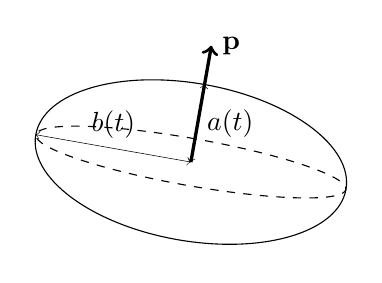
\begin{tikzpicture}[rotate=80]
        \draw(0,0) ellipse (1 cm and 2 cm);
        \draw[dashed](0,0) ellipse (0.3 cm and 2 cm);
        \draw[<->,very thin](0,0) --++ (1,0)node[midway,right]{$a(t)$};
        \draw[->,very thick](0,0) --++ (1.5,0)node[right]{$\textbf{p}$};
        \draw[<->,very thin](0,0) --++ (0,2)node[midway,above]{$b(t)$};
    \end{tikzpicture}
    \hfill
    \caption{Scheme of an  oblate spheroid oriented along the unit vector \textbf{p}.}
    \label{fig:scheme2}
\end{figure}
This tensor is defined such that its eigenvalues are the dimensionless square length of the semi-axis of the spheroid, such that $\textbf{C}_\alpha = a^2/r_0^2 \textbf{pp} + b^2 /r_0^2 (\textbf{I}-\textbf{pp})$ where $r$ is the radius of the sphere of same volume. 
This definition is convenient since it can be shown that $\textbf{C}_\alpha$ is equivalent to the Cauchy strain tensor well-defined in solid mechanics \citet{mwasame2017macroscopic}. 
Therefore, in a general coordinate system the point on the surface of the spheroid respect the equation, 
\begin{equation*}
    \textbf{r}\cdot\textbf{C}^{-1}\cdot\textbf{r} = r_0^2,
\end{equation*}
where $\textbf{C}$ is the inverse operator. 

Additionally, one can verify that the second order moment of mass of the particles is related to the conformation tensor through, $\textbf{M}_\alpha = \frac{m_\alpha  r_0^2}{5} \textbf{C}$. 
One can show that the constant volume constrain can be obtained by ensuring that $\text{det}(\textbf{C}) = (ab^2)^2 /(r_0^6) = 1$. 
It must be understood that at equilibrium the particle reach a spherical shape and therefore has $\textsc{C} = \textbf{I}$. 

\subsubsection*{The drop internal kinematic equation}



The evolution of $\textbf{C}_\alpha$ and $\bm\Gamma_\alpha$ will be described by the second moment of mass and first moment of momentum equation.
Consequently, we must reformulate the terms in \ref{eq:dt_M_alpha} and \ref{eq:dt_P_alpha} in terms of $\textbf{C}_\alpha$ and $\bm\Gamma_\alpha$. 
The integrals constitutive of these moments equations can be written, 
\begin{align}
    \intO{(\textbf{rw}_2^0 )_{ij}+ (\textbf{w}_2^0 \textbf{r})_{ij}} 
    = \textbf{C}_{\alpha,ik} \cdot \bm\Gamma_{\alpha,kj}
    +  \bm\Gamma_{\alpha,ki} \cdot \textbf{C}_{\alpha,jk}
    % +  \bm\Gamma_{\alpha,ij} + \bm\Gamma_{\alpha,ij}
    \\
    \intO{\rho_2 \textbf{w}_{2,i}^0\textbf{w}_{2,j}^0}
    = \frac{m_\alpha a^2}{5}
        \bm\Gamma_{\alpha,lj}\bm\Gamma_{\alpha,ki} \textbf{C}_{\alpha,kl} 
        % + \bm\Gamma_{\alpha,kj}\bm\Gamma_{\alpha,ki} 
        % + f_\textbf{ww}(\textbf{u}_\alpha,\textbf{C}_\alpha,\bm\Gamma_\alpha,\textbf{u}_1,\bm \Gamma_1,\phi_2)
        + \intO{\rho_2\textbf{w}^s_2\textbf{w}^s_2}
    \\
    \label{eq:sigma_2_def}
    \intO{\bm\sigma_{2,ij}^0}
    =
    % -\intO{p_2^0} \textbf{I}_{ij}
    \mu_2 v_\alpha (\bm\Gamma_{\alpha,ij} + \bm\Gamma_{\alpha,ij})
    + \mu_2 \intS{\textbf{w}^s_{2,i}\textbf{n}_{2,j}+ \textbf{w}^s_{2,j}\textbf{n}_{2,i}}
    + \textbf{I}_{ij}\intO{p_2^0} 
    \\
    \label{eq:sigma_I_def}
    \intS{\bm\sigma_{I,ij}^0}
    = \frac{2 \gamma v_\alpha }{a} \textbf{I}_{ij} - \frac{4 \gamma v_\alpha }{5 a} \textbf{C}_{\alpha,ij}
    +\mathcal(|\textbf{C}|^2)\\
    \intS{\textbf{r}\bm\sigma_1^0\cdot \textbf{n}_2}
    = 
    \frac{1}{2}\intS{(\textbf{r}\bm\sigma_1^0-\bm\sigma_1^0\textbf{r})\cdot \textbf{n}_2}
    + \frac{1}{2}\intS{(\textbf{r}\bm\sigma_1^0+\bm\sigma_1^0\textbf{r})\cdot \textbf{n}_2}
    % \textbf{M}(\textbf{u}_\alpha,\textbf{C}_\alpha,\bm\Gamma_\alpha,\textbf{u}_1,\bm \Gamma_1,\phi_2)
\end{align}
First, as discussed above only the deforming motion contribute to the symmetric part of the moment of momentum, we could therefore express it explicitly in terms of the particle unknown. 
Regarding the first moment of the surface tension, it has been computed analytically carrying a surface integral on the ellipsoidal surface of the droplet. 
Since, the droplets remain spheroidal under small deformation we choose to approximate $\intS{\bm\sigma_I^0}$ with its first order Taylor series in $\textbf{C}_\alpha$ without lost of generality.
Note that our expression of $\intS{\bm\sigma_I^0}$ is in agreement with \citet{lhuillier1987phenomenology} if one account for the slight difference of his definition of the deformation tensor which is half of $\textbf{C}_{\alpha}$. 
% in which our $\textbf{C}_\alpha$ is twice his, in the limit of small \textbf{C}_\alpha.
For the expression of $\intO{\rho_2 \textbf{w}_{2,i}^0\textbf{w}_{2,j}^0}$, $ \intO{\bm\sigma_{2,ij}^0}$ we had to introduce two unknown functions, $f_\textbf{ww}$, $f_{\bm{\sigma}}$, which vanish when $\textbf{w}^s_2 =0$. 
Therefore, these expressions are a sum of a function involving $\bm\Gamma_\alpha$ and an unknown part which depend on the parameters of the problem and need to be closed. 
The expression of $\intO{\rho_2 \textbf{w}_{2,i}^0\textbf{w}_{2,j}^0}$, $ \intO{\bm\sigma_{2,ij}^0}$ and $\intS{\textbf{r}\bm\sigma_1^0\cdot \textbf{n}_2}$ are very problem dependent. 
To provide a clearer example we computed these terms in \ref{ap:Translating_sphere} in the simplified scenario of an isolated droplet in a general linear flow. 
\begin{multline}    
    \frac{m_\alpha a^2}{10}\ddt^2 \textbf{C}_\alpha
    - \frac{m_\alpha a^2}{5}
    \bm\Gamma_{\alpha,lj}\bm\Gamma_{\alpha,ki} \textbf{C}_{\alpha,kl} 
    - \intO{\rho_2\textbf{w}^s_2\textbf{w}^s_2}\\
    + \mu_2 v_\alpha (\bm \Gamma_{p,ij}+\bm \Gamma_{p,ji})
    + \mu_2 \intS{\textbf{w}^s_{2,i}\textbf{n}_{2,j}+ \textbf{w}^s_{2,j}\textbf{n}_{2,i}}\\
    + \textbf{I}_{ij}\intO{p_2^0} 
    + \frac{2 \gamma v_\alpha }{a} \textbf{I}_{ij} 
    - \frac{4 \gamma v_\alpha }{5 a} (\textbf{C}_{ij} - \textbf{I}_{ij})
    =  
    + \frac{1}{2}\intS{(\textbf{r}\bm\sigma_2^0+ \bm\sigma_2^0\textbf{r})\cdot \textbf{n}}
\end{multline}
\begin{multline}    
    \frac{m_\alpha a^2}{10}\ddt^2 \textbf{C}_\alpha
    - \frac{m_\alpha a^2}{5}
    \bm\Gamma_{\alpha,lj}\bm\Gamma_{\alpha,ki} \textbf{C}_{\alpha,kl} 
    - \intO{\rho_2\textbf{w}^s_2\textbf{w}^s_2}\\
    + \mu_2 v_\alpha (
        \ddt \textbf{C}_{\alpha,ij}
         -(\textbf{C}_{\alpha,ik} - \textbf{I}_{ik}) \cdot \bm\Gamma_{\alpha,kj}
    -  \bm\Gamma_{\alpha,ki} \cdot (\textbf{C}_{\alpha,jk} - \textbf{I}_{\alpha,jk})
    )
    + \mu_2 \intS{\textbf{w}^s_{2,i}\textbf{n}_{2,j}+ \textbf{w}^s_{2,j}\textbf{n}_{2,i}}\\
    + \textbf{I}_{ij}\intO{p_2^0} 
    + \frac{2 \gamma v_\alpha }{a} \textbf{I}_{ij} 
    - \frac{4 \gamma v_\alpha }{5 a} (\textbf{C}_{ij} - \textbf{I}_{ij})
    =  
    + \frac{1}{2}\intS{(\textbf{r}\bm\sigma_2^0+ \bm\sigma_2^0\textbf{r})\cdot \textbf{n}}
\end{multline}
In the quasi steady regime all the derivative cancel out and $\bm\Gamma$ also,
\begin{multline}    
    % \frac{m_\alpha a^2}{10}\ddt^2 \textbf{C}_\alpha
    % - \frac{m_\alpha a^2}{5}
    % \bm\Gamma_{\alpha,lj}\bm\Gamma_{\alpha,ki} \textbf{C}_{\alpha,kl} 
    - \intO{\rho_2\textbf{w}^s_2\textbf{w}^s_2}
    + \mu_2 \intS{\textbf{w}^s_{2,i}\textbf{n}_{2,j}+ \textbf{w}^s_{2,j}\textbf{n}_{2,i}}\\
    + \textbf{I}_{ij}\intO{p_2^0} 
    + \frac{2 \gamma v_\alpha }{a} \textbf{I}_{ij} 
    - \frac{4 \gamma v_\alpha }{5 a} (\textbf{C}_{ij} - \textbf{I}_{ij})
    =  
    + \frac{1}{2}\intS{(\textbf{r}\bm\sigma_2^0+ \bm\sigma_2^0\textbf{r})\cdot \textbf{n}}
\end{multline}
Thus the stresslet might be computed upon known these integral but at this stage we could say ok just compute the stress let then. 
For bubbly flow we have the relation,
\begin{equation*}
+ \textbf{I}_{ij}\intO{p_2^0} 
+ \frac{2 \gamma v_\alpha }{a} \textbf{I}_{ij} 
- \frac{4 \gamma v_\alpha }{5 a} (\textbf{C}_{ij} - \textbf{I}_{ij})
=  
+ \frac{1}{2}\intS{(\textbf{r}\bm\sigma_2^0+ \bm\sigma_2^0\textbf{r})\cdot \textbf{n}}
\end{equation*}
In which case \textbf{C} is related to the pressure jump plus the stresslet while $\bm\Gamma$ isn't necessarily negligible. 

In this casethe stresslet appear to be, 
\begin{equation*}
    + \textbf{I}_{ij}\intO{p_2^0} 
    + \frac{2 \gamma v_\alpha }{a} \textbf{I}_{ij} 
    - \frac{4 \gamma v_\alpha }{5 a} (\textbf{C}_{ij} - \textbf{I}_{ij})
    - \mu_1 \intS{\textbf{w}^s_{2,i}\textbf{n}_{2,j}+ \textbf{w}^s_{2,j}\textbf{n}_{2,i}}
    - \mu_1 v_\alpha (\bm \Gamma_{p,ij}+\bm \Gamma_{p,ji})
    =  
    \intS{\textbf{r}\bm\sigma_2^0\cdot \textbf{n}}
    - \mu_1 \intO{e_2^0}
\end{equation*}
Then if we arrive to prove that $(\textbf{C}_{ij} - \textbf{I}_{ij}):\textbf{I}_{ij} = 0$ we recover a Laplace pressure like making $+ \textbf{I}_{ij}\intO{p_2^0} 
+ \frac{2 \gamma v_\alpha }{a} \textbf{I}_{ij} $ equal to the fluid pressure. 

At this point it wouldn't be wise trying to find an expression for each of these unknown functions in such a generality. 
Instead, we expose the unclosed set of equation of motions for spheroidal particles. 
In addition to the previously exposed equations (mass, momentum and energy equation) this system is constituted of three equations, one for $\textbf{C}_\alpha$ and two equation for the moment of momentum, the symmetric and skew-symmetric moment of momentum. 
% These read, 
% \begin{align*}
%     \ddt \textbf{C}_{\alpha,ij}
%     = \textbf{C}_{\alpha,ik} \cdot \bm\Gamma_{\alpha,kj}
%     +  \bm\Gamma_{\alpha,ki} \cdot \textbf{C}_{\alpha,jk},\\
%     \frac{a^2  m_\alpha}{5} \ddt( \textbf{C}_{ik} \cdot \bm\Gamma_{\alpha,kj}
%     -  \bm\Gamma_{\alpha,ki} \cdot \textbf{C}_{jk})
%     =  \intS{(\textbf{r}\bm\sigma_2^0- \bm\sigma_2^0\textbf{r})\cdot \textbf{n}}\\
%     \frac{m_\alpha a^2}{5}\ddt^2 \textbf{C}_\alpha
%     - \frac{m_\alpha a^2}{5}[
%     \bm\Gamma_{\alpha,lj}\bm\Gamma_{\alpha,ki} \textbf{C}_{\alpha,kl} + f_\textbf{ww}]
%     + \mu_2 v_\alpha [(\bm \Gamma_{p,ij}+\bm \Gamma_{p,ji})
%     + f_{\bm{\sigma}}]\\
%     + \frac{2 \gamma v_\alpha }{a} \textbf{I}_{ij} 
%     - \frac{4 \gamma v_\alpha }{5 a} (\textbf{C}_{ij} - \textbf{I}_{ij})
%     = \intS{(\textbf{r}\bm\sigma_2^0+ \bm\sigma_2^0\textbf{r})\cdot \textbf{n}}
%     % + \textbf{I}_{ij}\intO{p_2^0}
% \end{align*}
% Where we placed the unknown function at the right hands side of these equations. 
Now, we would like to propose a more intuitive interpretation of the mass and momentum equations.
To that end, we make the problem dimensionless by introducing, 
the \textit{Capillary number} $Ca= \frac{\mu_1 U}{\gamma}$, The viscosity ratio $\lambda = \mu_2/\mu_1$, the density ratio $\zeta = \rho_2/\rho_1$ and the Reynolds number $Re = \frac{a U \rho_1}{\mu_1}$, with $U$ as the velocity scale. 
%  such that  $\bm\Gamma_\alpha'  = \frac{a}{U}\bm\Gamma$, and $\tau_a$ the timescale related to the drop shape evolution.
In the low Reynolds regime the first moment of surface traction forces will be proportional to a viscous stress (see \ref{ap:Translating_sphere}), therefore :$\intS{\textbf{r}\bm\sigma_2^0\cdot \textbf{n}} =\mu_1  \tau v_\alpha \intS{\textbf{r}\bm\sigma_2^0\cdot \textbf{n}}^*$, with $\tau$ the inverse timescale of the external solicitation.
The ratio between the external flow scale $\tau$ and the drop timescale $\tau_a$ is noted $\beta$. 
With that in mind, \ref{eq:dt_M_alpha}, \ref{eq:dt_mu_alpha} and \ref{eq:dt_S_alpha} might be written :
\begin{align}
    \label{eq:dt_Cs}
    \beta \ddt \textbf{C}_{\alpha,ij}
    - \textbf{C}_{\alpha,ik} \cdot \bm\Gamma_{\alpha,kj}^*
    - \bm\Gamma_{\alpha,ki}^* \cdot \textbf{C}_{\alpha,jk},
    = 
    \bm\Gamma_{\alpha,ij}^*
    +  \bm\Gamma_{\alpha,ji}^*\\
    Re \zeta \beta \ddt( \textbf{C}_{\alpha,ik} \cdot \bm\Gamma_{\alpha,kj}^*
    -  \bm\Gamma_{\alpha,ki}^* \cdot \textbf{C}_{\alpha,jk}
    + \bm\Gamma_{\alpha,ji} - \bm\Gamma_{\alpha,ij})
    =  \intS{(\textbf{r}\bm\sigma_2^0- \bm\sigma_2^0\textbf{r})\cdot \textbf{n}}^*\\
    \zeta Re \frac{1}{5}  
    \left[
        \frac{1}{2}\beta^2 \ddt^2_* \textbf{C}_\alpha
        - \bm\Gamma_{\alpha,lj}^* \bm\Gamma_{\alpha,ki}^* \textbf{C}_{\alpha,kl}^* 
        - \bm\Gamma_{\alpha,kj}^* \bm\Gamma_{\alpha,ki}^* 
        - f_\textbf{ww}
    \right]\nonumber\\
    + \lambda \left[
        \beta \ddt \textbf{C}_{\alpha,ij}
        -\textbf{C}_{\alpha,ik} \cdot \bm\Gamma_{\alpha,kj}
        - \bm\Gamma_{\alpha,ki}^* \cdot \textbf{C}_{\alpha,jk},
        + f_{\bm{\sigma}}
    \right]\nonumber\\
    - \frac{1}{Ca}\left[
        \frac{4}{5} \textbf{C}_{\alpha,ij}
        +2 \textbf{I}_{ij} 
    \right]
    =
    \frac{1}{2}\intS{(\textbf{r}\bm\sigma_1^0+ \bm\sigma_1^0\textbf{r})\cdot \textbf{n}}^*
    \label{eq:dt2_C}
\end{align}







The drop internal velocity will be assumed to be linear and homogeneous such as if it was a solid deformable displacement. 
It must be said that due to the presence of surface tension and relative velocity this hypothesis isn't physical. 
Indeed, on one hand inhomogeneous stresses such as surface tension stress, might induce inhomogeneous internal flow \citep{goddard1967nonlinear}, and obviously the relative motion will evidently induce a Hill's vortex-like internal motions. 
Therefore, in a second step the modeling of internal flow will include quadratic terms but for ow we restrict our attention to linear internal flow fields. 
Taking into account this assumption the drop internal velocity field can be written,
\begin{equation}
    \textbf{w}_2^0(\textbf{x}_\alpha)
    = \bm\Gamma_\alpha \cdot \textbf{r}
    =\bm{\Omega}_\alpha\cdot \textbf{r}
    + \textbf{E}_\alpha \cdot \textbf{r}
    \label{eq:def_vel}
\end{equation}
where $\bm\Gamma_\alpha$, is the velocity gradient for any point inside the domain $\Omega_\alpha(t)$, and $\textbf{E}_\alpha$ represents the rate of strain or the symmetric part second order tensor, and $\bm\Omega_\alpha$ the angular velocity pseudo vector. 

The evolution of the internal kinematic of the droplet, i.e. the shape, will be described by the second moment of mass equation, to which we substitute the tensor $\mathcal{M}_\alpha$ by \textbf{C} to obtain an equation for the deformation. 
It yields, 
\begin{equation*}
    \ddt \textbf{C}_{ij}
    = \textbf{C}_{ik} \cdot \bm\Gamma_{\alpha,kj}
    +  \bm\Gamma_{\alpha,ki} \cdot \textbf{C}_{jk}.
    \label{eq:dt_C}
\end{equation*}
From this point one can relate $\bm\Gamma_{\alpha,kj}$ to the fluid mean kinematic properties. 
In pure shear flow for example, if one consider the problem of a slightly deformable droplet one can show that, $\bm\Gamma \sim \Gamma_1(\textbf{x}_\alpha)$ where $\bm\Gamma_1$ is the local fluid velocity gradient.
From this consideration one can find back the classical models such as the one of  \citet{maffettone1998equation,schowalter1968rheological}. 

In our current problem, rising inertial droplets, we must thus seek for an expression linking the drop internal velocity gradient $\bm\Gamma_\alpha$ with the relative motion $\textbf{u}_{pf}$. 
This is done through the consideration of the second moment of momentum equation. 

\subsubsection*{The dynamical droplet equations}

Objective : 
\begin{equation*}
    \bm\sigma 
    = 
    - \phi_1 p_1 \textbf{I}
    - \mu_1 \textbf{e}
    + \phi_2(\bm\sigma_2 - \bm\sigma_1)
    + \phi_I\bm\sigma_I
\end{equation*}

The dynamic of the droplet will be described by the use of the symmetric moment of momentum equation presented in \ref{sec:Lagrangian}.
We will therefore need constitutive equation for the particle internal and surface stress. 
The particle internal stress is described by a Newtonian behavior law yielding directly, 
\tb{hypothèse}
\begin{equation*}
    \intO{\bm\sigma_2^0}
    = - \intO{p_2^0} \delta_{ij}
    + v_\alpha \mu_2 \textbf{E}_{\alpha,ij}.
\end{equation*} 
Equally, if the particle were constituted of any other material one could include the adapted constitutive law in this term. 
Regarding the particle surface stress, it can be computed analytically since we assumed a spheroidal shape. 
% Indeed, all the points on the surface of the particle can describe by the equation, $\textbf{r}\cdot\textbf{C}^{-1}-1=0$ which mean that the normal vector at the surface can be express as $\textbf{n}_2 = 2\textbf{H}\cdot\textbf{r}$ and it follow the tensorial expression of the local stress. 
The details are not given here but the results at $\mathcal{O}(|\textbf{C}|^3)$  and $\mathcal{O}(|\textbf{C}|^2)$ accurate yield, 
\begin{align*}
    \pSavg{\bm\sigma_I^0}
    &= \frac{\gamma v 2}{r} \left[
        1  + \frac{1}{20 } (\textbf{C}_{-\textbf{I}}:\textbf{pp})^2 
        + \frac{4}{20 } [\textbf{C}_{-\textbf{I}}:(\textbf{I}-\textbf{pp})]^2\right] \textbf{I}\\
        &- \frac{\gamma v}{35 r} \left[ 28 \textbf{C}_{-\textbf{I}}
        + 4[\textbf{C}_{-\textbf{I}}\cdot \textbf{C}_{-\textbf{I}} + 15 (\textbf{C}_{-\textbf{I}}:\textbf{pp})^2\textbf{pp}]
        \right]
        +\mathcal{O}(|\textbf{C}|^3)\\
    &= \frac{\gamma v 2}{r} \textbf{I} - \frac{\gamma v 4}{5 r} (\textbf{C} - \textbf{I})
    +\mathcal(|\textbf{C}|^2)
\end{align*}
Notice that the first term of the first equality correspond to $\frac{2\gamma}{3}s_\alpha$, it is therefore $\frac{2}{3}$ of the surface energy which varies only at $\mathcal{O}(|\textbf{C}|^2)$. 
The second term account for the deviatoric part of the stress tensor which is of $\mathcal{O}(\textbf{C})$. 
The results at first order are agreements with \citet{lhuillier1987phenomenology} when accounting for the different definition of the conformation tensor \textbf{C} that he used.

The moment of momentum equation with an internal velocity such as it is described by \ref{eq:def_vel} is then given by the expression,
\begin{multline}
    \ddt (\textbf{C}_{\alpha,ik} \bm\Gamma_{\alpha,kj})
    -\bm\Gamma_{\alpha,lj}\bm\Gamma_{\alpha,ki} \textbf{C}_{\alpha,kl}
    = 
    % \intO{p_2^0} \delta_{ij}
    - \frac{5\mu_2}{a^2\rho_2}  \textbf{E}_{\alpha,ij}
    + \frac{\gamma 6 }{\rho_2 a^3} \textbf{I} 
    - \frac{\gamma 4}{\rho_2 a^3} \textbf{C}_{\alpha,ij} 
    +\frac{5}{a^2 \rho_2 v_\alpha} \pavg{\textbf{r}\bm\sigma_1^0\cdot\textbf{n}_2}_{ij},
    \label{eq:moment_of_momentum}
\end{multline}
Or its symmetric part,
\begin{multline}
    \ddt^2 (\textbf{C}_{\alpha,ik})
    - 2\bm\Gamma_{\alpha,lj}\bm\Gamma_{\alpha,ki} \textbf{C}_{\alpha,kl}
    = 
    % \intO{p_2^0} \delta_{ij}
    - 2\frac{5\mu_2}{a^2\rho_2}  \textbf{E}_{\alpha,ij}
    + 2\frac{\gamma 6 }{\rho_2 a^3} \textbf{I} 
    - 2\frac{\gamma 4}{\rho_2 a^3} \textbf{C}_{\alpha,ij} 
    + 2\frac{5}{a^2 \rho_2 v_\alpha} \pavg{\textbf{r}\bm\sigma_1^0\cdot\textbf{n}_2}_{ij},
    \label{eq:moment_of_momentum}
\end{multline}
\tb{The internal velocity is way more to complicated one must use Hill vortex}
\tb{The isotropic part might cancel the difference in pressure.}
where the only undetermined term is the first moment of the hydrodynamic forces. 
While deriving \ref{eq:moment_of_momentum} we made absolutely no hypothesis on the dilute nature of the flow nor on its potentially inertial effect.
Therefore, solely the first moment of hydrodynamic force might be able to take in account the effect of finite volume fraction, inertial effect, particle interaction\ldots
Therefore we introduce the function,
\begin{align*}
    \pavg{\textbf{r}\bm\sigma_1^0\cdot\textbf{n}_2}_{ij}
    = \textbf{f}_{1,ij}(\textbf{u}_\alpha - \textbf{u}_1,\bm\Gamma_\alpha - \bm\Gamma_1, \textbf{C}_{\alpha},Re,\phi) 
\end{align*}
which depends on the particles fluid relative properties, $(\textbf{u}_\alpha - \textbf{u}_1,\bm\Gamma_\alpha - \bm\Gamma_1)$ and problem dimensionless number $Re,\phi$. 
Such a relation have been found in \citet{goddard1967nonlinear}. 

In \citet{raja2010inertial} they consider a deformable drop in shearing inertial flow. 
Their expression (3.18) for the particle contribution to the suspension stress is in fact a combination of \ref{eq:moment_of_momentum} and \ref{eq:dt_C} where the first moment $\pavg{\textbf{r}\bm\sigma_1^0\cdot\textbf{n}_2}_{ij}$ have been solved analytically in terms of $\bm\Gamma_1$.

Therefore, in the continuity of their work we now wish to determine $\pavg{\textbf{r}\bm\sigma_1^0\cdot\textbf{n}_2}_{ij}$ in a pure translating motion with no mean shear. 
It is known from the singularity solution of stokes flow that $\pavg{\textbf{r}\bm\sigma_1^0\cdot\textbf{n}_2}_{ij} = 0$ for a non-inertial spherical droplet in pure translation. 
However, when finite inertia effects appear the first moments of surface traction is not null and the drop deform into a spheroid proportionally the relative velocity $\textbf{u}_{fp}$. 


\subsubsection*{Determination of the shape based on \citet{taylor1964deformation} theoretical results}

In the last section we assumed an arbitrary spheroidal drop within a suspension. 
Now we consider that the drop is only subject to a relative motion with the fluid. 
Our goal is still to express the stress within the suspension. 

In \citet{taylor1964deformation} they derive the shape and the drag force of a translating droplet at $\textbf{O}(Re^2)$ in a steady state situation. 
Although they did not directly derive the stress let they provide a formula for the shape as a function of the relative velocity. 
In \citet{taylor1964deformation} they give an explicit formula for the deformation in terms of the Reynolds number $Re$ based on the relative velocity fields, $\textbf{u}_\alpha - \textbf{u}_1$. 
The dimensionless radius of the droplets can be express in the polar coordinate reference frame of the drop as, 
\begin{equation*}
    \frac{R_\text{taylor}(\theta)}{a} = 1 - \beta \textit{We} P_2(\cos\theta)
    + \mathcal{O}(Re^3)
\end{equation*}
where $Re = |\textbf{u}_{pf}| a /\nu_1$, $P_2(\cos\theta)$ is the Legendre polynomial of degree two and $\kappa$ is a coefficient related to physical parameters given in \citet{taylor1964deformation}.  
This solution need to satisfy $\kappa Re \ll 1$ and $Re \ll 1$ to be valid. 
These, 
% \begin{center}
%     \begin{tikzpicture}[gradient arrow/.style={
%         insert path={coordinate[pos=#1,sloped,
%             above=\pgfkeysvalueof{/tikz/ga/above}]  (aux-1)
%            coordinate[pos=#1,sloped,
%             above=\pgfkeysvalueof{/tikz/ga/above}+\pgfkeysvalueof{/tikz/ga/length}] (aux-2)
%            (aux-1) edge[/tikz/ga/arrow] 
%            (aux-2)}},ga/.cd,
%            above/.initial=3pt,
%            length/.initial=12pt,
%            arrow/.style={-stealth,black,solid,thick}]
%          \begin{axis}[scale=0.85,xmin=-4,xmax=12, ymin=-4,ymax=4,x=1cm,y=1cm,at={(-4cm,-4cm)}]
%           \addplot +[no markers,name=contour,
%            raw gnuplot,
%            thick,dashed,
%            empty line = jump, % not strictly necessary, as this is the default behaviour in the development version of PGFPlots
%            ] gnuplot {
%                set contour base;
%                set cntrparam levels discrete -2,-1.1,-1.4;
%                unset surface;
%                set view map;
%                set isosamples 500;
%                set samples 500;
%                splot -2/sqrt((x-7.5)^2+y^2)-3/sqrt((x-0.5)^2+y^2);
%            } 
%         %    [pos segment=1]
%         %    [gradient arrow/.list={0.2,0.8}]
%         %    [pos segment=3,/tikz/ga/arrow/.append style={red},/tikz/ga/length=10pt]
%         %    [gradient arrow/.list={0.2,0.8}];
%          \end{axis}
%     \end{tikzpicture}
% \end{center}
Upon assuming a quasi steady state regime which correspond to a droplet response time $\frac{1}{\tau_a^2} \ll \frac{\mu_1 U \lambda }{a^3\rho_2} \approx \frac{\mu_1 U \lambda }{a^3\rho_2 Ca} \approx \frac{\mu_1 U \lambda }{a^3\rho_2}$ we can stipulate that the shape of the droplet is instantaneously correlated with the velocity. 
In this hypothesis it is clear that the shape of the droplet is correlated at any time with the local motion of the flow $\textbf{u}_{fp}$. 
The conformation tensor principal values, are related to \citet{taylor1964deformation} formula through,
\begin{align*}
    \textbf{C}(\textit{We})
    % = \left(\frac{R_\text{taylor}(0)}{a}\right)^2
    = (1 - \beta \textit{We} )^2 \textbf{pp}
    + 
     (1 + \beta \textit{We}/2  )^2 (\textbf{I}-\textbf{pp})
\end{align*}
where $\textit{We}$ is the \textit{Weber} number defined as $\textit{We} = \rho_1 a \textbf{u}_{\alpha f}\cdot\textbf{u}_{\alpha f}/\sigma$. 

Now that we obtained the shape as a function of the relative velocity, we aim to recover the rate of deformation of the drop through the second moment of mass equation. 
The droplet interior flow is a complex function of space and time. 
We assumed small deformation such that our spherical particle become a spheroid. 
Therefore, the velocity fields responsible for the shape change is a linear function of the position, thus $\textbf{w}_2^0 = f(\textbf{r}) + \bm\Gamma_\alpha(t,\FF) \cdot \textbf{r}$, where $f(\textbf{r})$ is the steady state internal motion and $\bm\Gamma_\alpha(t,\FF)$ is a time dependent matrix describing the homogeneous deformation of the droplets. 
The complex recirculation structure such as Hill vortexes-like doesn't contribute to the symmetric part of the moment of momentum as it is not changing the shape of the particle. 
The only contribution to the stretching of momentum is therefor the second term. 
Additionally, we always consider the drop deformation in the direction of the flow. 
Now that the drop shape is fully determined by the local Reynolds number the second order of mass equation can be use to determine the inner rate of strain of the drop,
\begin{equation*}
    \ddt \textbf{C}_{ij}
    = \textbf{C}_{ik} \cdot \bm\Gamma_{\alpha,kj}
    +  \bm\Gamma_{\alpha,ki} \cdot \textbf{C}_{jk}.
\end{equation*}
This equation must be solved for the $\Gamma_{ki}$ as $\textbf{C}$ is a known function of $\textbf{u}_{pf}$ and the physical parameters. 

As mentioned above the surface tension stress can be estimated to be an instantaneous function of \textbf{C}, namely, 
\begin{align*}
    \pSavg{\bm\sigma_I^0}
    = \frac{\gamma v 2}{r} \textbf{I} - \frac{\gamma v 4}{5 r} (\textbf{C} - \textbf{I})
    +\mathcal(|\textbf{C}|^2)
\end{align*}
At this stage the only remaining term to determine the contribution to the suspension stress is an expression of the particle stress tensor as a function of \textbf{C} ad $\bm\Gamma$. 
The symmetric part of the moment of momentum equation can be written,
\begin{equation*}
    \ddt^2\intO{\textbf{C}_{ij}}
    -\intO{\rho_2\textbf{w}_{2,i}^0\textbf{w}_{2,j}^0}
    + \intO{\bm\sigma_{2,ij}^0}
    + \intS{\bm\sigma_{I,ij}^0}
    = \intS{(\textbf{r}\bm\sigma_1^0+ \bm\sigma_1^0 \textbf{r})_{ijk}\cdot \textbf{n}_{2,k}}
\end{equation*}
At this stage we must either find the complete closure for $\textbf{w}_{2,i}^0$ which will enable us to find an expression for one of the two remaining terms.
And by solving this equation one might obtain the last one terms in terms of $\bm\Gamma$ and \textbf{C}. 
\tb{Either find the singularity sol or assume linear displacement}

We're assuming that the rate of strain is the only contribution to the stress, which might be justified by the fact that Hill's vortexes resultant vanish for spherical drops. 
Thus, the drop interior stress might be written, 
\begin{equation*}
    \pSavg{\bm\sigma_2^0}
    =-\pOavg{p_2^0} 
    + \mu_2 n_p (\bm\Gamma_{p,ij}+\bm\Gamma_{p,ji})
\end{equation*}
Then the set of equation needed to describe the rheology of a dilute suspension of inertial drops is, 
\begin{align*}
    \textbf{C}_p(\textit{We})
    % = \left(\frac{R_\text{taylor}(0)}{a}\right)^2
    = (1 - \beta \textit{We} )^2 \textbf{pp}
    + 
     (1 + \beta \textit{We}/2  )^2 (\textbf{I}-\textbf{pp})\\
    \pavg{\ddt \textbf{C}_{ij}}
    = \textbf{C}_{p,ik} \cdot \bm\Gamma_{p,kj}
    +  \bm\Gamma_{p,ki} \cdot \textbf{C}_{p,jk}.\\
    \bm\sigma^\text{dev}
    = 
    \mu_1 \textbf{e}_{ij}
    +  n_p (\mu_2 - \mu_1) (\bm\Gamma_{p,ij} + \bm\Gamma_{p,ji})
    + n_p \frac{\gamma  4}{5 r} (\textbf{C}_{p,ij} - \textbf{I}_{ij})
\end{align*}

Under this assumption it is observed that $\textbf{C}\sim U^2$ has the same form as the pseudo turbulence Reynolds stress computed in potential flow. 
Indeed, 
The deviatoric part of the conformation tensor can be written exactly as, 
\begin{equation*}
    \textbf{C} - \textbf{I}  = - 3 \beta \textit{We} \textbf{pp} +  \beta \textit{We} \textbf{I}
    + (\beta^2 \textit{We}^2 3/4) \textbf{pp} + \beta^2 \textit{We}^2/4 \textbf{I} 
\end{equation*}
We now stipulate that the deformation occur in the direction of the velocity difference such that the relative phase velocity of the particle $\alpha$ is written, $\textbf{u}_{\alpha f} = |\textbf{u}_{\alpha f}|\textbf{p}$, in this case the conformation tensor can be expressed, 
\begin{equation}
    \textbf{C}(\textbf{u}_{\alpha f}) - \textbf{I}  =  \frac{ \rho_1 a \beta}{\gamma} \left[
        -  3
        \textbf{u}_{\alpha f}\textbf{u}_{\alpha f}+   \textbf{u}_{\alpha f}\cdot\textbf{u}_{\alpha f}\textbf{I}
    \right]
    +\textbf{u}_{\alpha f}\cdot\textbf{u}_{\alpha f}\left(\frac{ \beta \rho_1 a}{\gamma}\right)^2
    \left[
        \frac{3}{4}
        \textbf{u}_{\alpha f}\textbf{u}_{\alpha f}
        +
        \frac{1}{4}
        \textbf{u}_{\alpha f}\cdot\textbf{u}_{\alpha f}
        \textbf{I}
    \right]
    \label{eq:C_def_with_u}
\end{equation}
This tensor is the particle confirmation tensor of the particle $\alpha$. 
We now apply an average procedure, and by that, $\pavg{\textbf{u}_{\alpha f}\textbf{u}_{\alpha f}} = \textbf{u}_{pf}\textbf{u}_{pf} + \pavg{\textbf{u}_\alpha'\textbf{u}_\alpha'}$ to gather with the assumption that the higher order fluctuation terms becomes negligible we obtain, 
\begin{multline*}
    \textbf{C}_p - \textbf{I}  =  \frac{ \rho_1 a \beta}{\gamma} \left[
        -  3
        \textbf{u}_{\alpha f}\textbf{u}_{\alpha f}
        +   (\textbf{u}_{\alpha f}\cdot\textbf{u}_{\alpha f})\textbf{I}
    \right]\\
    +\textbf{u}_{\alpha f}\cdot\textbf{u}_{\alpha f}\left(\frac{ \beta \rho_1 a}{\gamma}\right)^2
    \left[
        \frac{3}{4}
        \textbf{u}_{p f}\textbf{u}_{p f}
        +
        \frac{1}{4}
        (\textbf{u}_{p f}\cdot\textbf{u}_{p f})
        \textbf{I}
    \right]
    + \pavg{\textbf{C}(\textbf{u}_\alpha')}
\end{multline*}
where the last term correspond to \ref{eq:C_def_with_u} with $\textbf{u}_\alpha'$ is input velocity. 
Under these quite restrictive assumption we have shown that the surface tension contribution to the bulk stress have the same functional form as the Reynolds stress in potential flows \citet{van1982bubble}. 
% 
\subsection{Deformable rising droplets}

In a suspension of deformable particles it is known that the drag force is a function of the shapes of the drops.
To take in account such parameter in averaged models one usually use a force correlation function of the Capillary or Morton number. 
However, such models are valid in very specific scenario and flow condition. 
Another way to take in account the particles' deformation or aspect ratio, would be to solve an equation for the mean particle shapes. 
Then, one can create a drag force closure for various particles' aspect ratio. 

\begin{figure}[h!]
    \centering
    \hfill
    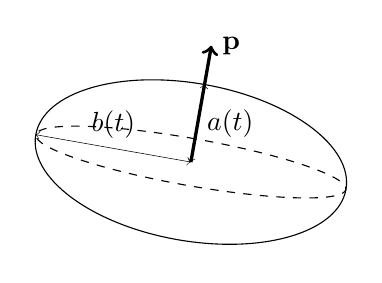
\begin{tikzpicture}[rotate=80]
        \draw(0,0) ellipse (1 cm and 2 cm);
        \draw[dashed](0,0) ellipse (0.3 cm and 2 cm);
        \draw[<->,very thin](0,0) --++ (1,0)node[midway,right]{$a(t)$};
        \draw[->,very thick](0,0) --++ (1.5,0)node[right]{$\textbf{p}$};
        \draw[<->,very thin](0,0) --++ (0,2)node[midway,above]{$b(t)$};
    \end{tikzpicture}
    \hfill
    \caption{Scheme of an  oblate spheroid oriented along the unit vector \textbf{p}.}
    \label{fig:scheme2}
\end{figure}
We consider in this problem an oblate spheroid with a time dependent aspect ratio $\chi = a(t)/b(t)$ oriented along the unit vector \textbf{p}, see \ref{fig:scheme2}.
In this context an equation describing the droplets surface can be found in the reference frame of the droplets, namely, 
\begin{equation}
    \mathscr{F}
    = \textbf{r}\cdot \textbf{H}\cdot \textbf{r} - a_0^2 = 0 
    \label{eq:F_def}
\end{equation}
where \textbf{H} is a symmetric traceless tensor such that $\textbf{H} = \textbf{pp} (a_0/a(t))^2 + (\textbf{I}- \textbf{pp})(a_0/b(t))^2$. 

We consider a mono disperse suspension of droplet with constant mass. 
The objective of this section is to derive constitutive equations to predict the mean orientation, and mean aspect ratio of the droplet. 

\subsubsection{Particle's internal motion}

In the first place we assume a linear homogeneous particle internal motion, such as, 
\begin{equation}
    \textbf{w}_2^0(\textbf{x}_\alpha+ \textbf{r})
    = 
    + \textbf{r} \cdot \textbf{D}_\alpha
    = 
    \bm{\omega}_\alpha \times \textbf{r} 
    + \textbf{r} \cdot \textbf{E}_\alpha
\end{equation}
where $\bm{\omega}_\alpha$ is the angular velocity of the particle, $\textbf{E}_\alpha$ is the mean deformation gradient. 
% Note that the second rank tensor $\textbf{U}_\alpha = \bm{\}$
To respect the mass conservation condition, i.e. $\div \textbf{w}_2^0 =0$, The mean gradient deformation $\textbf{E}_\alpha$ has to respect the conditions : $\textbf{E}_\alpha:\textbf{I}=0$. 
The assumption of linear internal motion is wrong for droplets and bubbles were we are clearly in presence of internal motions. 
However, for now these motions will be discarded. 

\subsubsection{Fundamental properties}

We now compute the mass, moment of mass and moment of momentum of this particle. 
The volume of an ellipsoid reads as, 
\begin{align}
    v_\alpha
    = \frac{4}{3}\pi a b^2
    = \frac{4}{3}\pi \chi  b^3
    \label{eq:volume_def}
\end{align}
Before going further we must say that the two radius $a(t)$ and $b(t)$ are actually dependent since one must preserve the total mass of the particle. 
We recall that we are in the context of mono disperse suspension such that the volume of the particles $v_\alpha$ is actually known, Thus, 
\begin{equation*}
    a(t) 
    = \frac{3 v_\alpha}{4 \pi b^2(t)}
    = \frac{r_0^3}{ b^2(t)}
    \Leftrightarrow
    b^2(t) 
    = \frac{r_0^3}{ a(t)}
\end{equation*}
Where $r_0$ is the radius of the sphere of same volume such as $v_\alpha = \frac{4}{3}\pi r_0^3$. 
Also, it might be useful to compute the relation between the derivative of the radius,  
\begin{equation*}
    \ddt v_\alpha 
    % = \ddt \frac{4}{3}\pi a b^2
    = \frac{4}{3}\pi \dot{a}(t) b^2(t)
    + \frac{8}{3} \pi {a}(t) b(t) \dot{b}(t)
    = 0 
    \Leftrightarrow
     \dot{a}(t)
    =  
    - 2 \frac{a(t)}{b(t)}  \dot{b}(t)
    % \Leftrightarrow
\end{equation*}
Which means that the derivative of both radius are related to twice the aspect ratio. 

The second moment of mass is somewhat more complicated to compute, we have, 
\begin{align*}
    \mathcal{M}_{\alpha,ij}
    = \int r_ir_j dxdydz
\end{align*}
At this stage we would like to compute the integral in spherical coordinate, thus we introduce the change of variables, 
\begin{align*}
    x' = x/a 
    && y' = y/b 
    && z' = z/b 
\end{align*}
By assuming that the spheroid is aligned with the $z$ axis and centered at the origin we get, 
\begin{align*}
    \mathcal{M}_{\alpha,zz}
    = a(t)^3 b(t)^2 \int z'z' dx'dy'dz'
\end{align*}
switching in spherical coordinate yields 
\begin{align*}
    \mathcal{M}_{\alpha,zz}
    = a(t)^3 b(t)^2 \int_0^1 \int_0^{2\pi}\int_0^\pi r^4 \cos^2\phi \sin\phi d\phi d\theta dr
    = a(t)^3 b(t)^2 \frac{1}{5}\frac{4}{3} \pi
    = v_\alpha \frac{a^2(t)}{5}\\
    \mathcal{M}_{\alpha,xx}
    = a(t) b(t)^4 \int_0^1 \int_0^{2\pi}\int_0^\pi r^4 \sin^3\phi\cos^2\theta d\phi d\theta dr
    = a(t) b(t)^4
    \frac{1}{5}
     \frac{4}{3}
     \pi
     =v_\alpha \frac{b^2(t)}{5}
\end{align*}
In a more general manner one can define the tensor $\mathcal{M}_\alpha$ in the laboratory reference frame using the orientation tensor \textbf{p}, such that, 
\begin{equation}
    5 \frac{\mathcal{M}_{\alpha,ij}}{v_\alpha}
    = p_i p_j 
    a^2(t) 
    + (\delta_{ij} - p_ip_j) b^2(t)
    = H_{ij}^{-1}
    \label{eq:M_alpha_def}
\end{equation} 
In light of \ref{eq:M_alpha_def}we reduced the description of any particle in our flow to four parameters, the 3 components of \textbf{p}, and the radius $a(t)$. 
It might be useful to make the inertia tensor dimensionless by dividing both sides by $r_0$, which gives, 
\begin{equation}
    5 \frac{\mathcal{M}_{\alpha,ij}}{v r_0^2}
    = p_i p_j 
    e_{||}^2(t) 
    + (\delta_{ij} - p_ip_j) 
    e_\bot^2(t) 
    \label{eq:M_alpha_def2}
\end{equation} 
Notice that since $ab^2 =r_0^3$ the deformation are related through $e_\bot = \frac{b}{a}r e_{||} =\frac{b^3}{r^2} e_{||} $


Now let's compute the first moment of momentum $\mathcal{P}_\alpha$, it reads, 
\begin{align*}
    \mathcal{P}_{\alpha,ij}
    = \int r_i w_{2,j}^0 d\Omega
    = D_{\alpha,jk} \mathcal{M}_{\alpha,ki}
    = \epsilon_{jkl} \omega_{\alpha,k} \mathcal{M}_{\alpha,il}
    +  E_{\alpha,jk} \mathcal{M}_{\alpha,ik}
\end{align*}
Taking the double contracted product with $\epsilon_{mij}$ of the moment of momentum yield the angular momentum equation, 
\begin{align*}
    \mu_{\alpha,m}
    = \epsilon_{mij}\mathcal{P}_{\alpha,ij}
    = \epsilon_{jmi} \epsilon_{jkl} \omega_{\alpha,k} \int r_i r_l  d\Omega
    +  \epsilon_{mij} E_{\alpha,jk} \int r_i r_k  d\Omega\\
    = (\delta_{mk}\mathcal{M}_{\alpha,ll} - \mathcal{M}_{\alpha,mk}) \omega_{\alpha,k}
    +  \epsilon_{mij} E_{\alpha,jk} \int r_i r_k  d\Omega\\
    = \mathcal{I}_{\alpha,mk} \omega_{\alpha,k}
    +  \epsilon_{mij} E_{\alpha,jk} \mathcal{M}_{\alpha,ik}\\
\end{align*}
The second contribution of the angular momentum would vanish if the particles where spherical. 
Lastly, the symmetric part of the moment of momentum reads, 
\begin{align*}
    2\mathcal{S}_{\alpha,ij}
    = \epsilon_{jkl} \omega_{\alpha,k} \mathcal{M}_{\alpha,il}
    + \epsilon_{ikl} \omega_{\alpha,k} \mathcal{M}_{\alpha,jl}
    +  E_{\alpha,jk} \mathcal{M}_{\alpha,ik}
    +  E_{\alpha,ik}  \mathcal{M}_{\alpha,jk}
\end{align*}

\subsubsection*{Evolution equation of a single particle shpae.}

We first start by the kinetic equations.  
In view of the previous expression the evolution equation of the momentum tensor is,  
\begin{equation*}
    \ddt {\mathcal{M}_{\alpha,ij}}
    + \epsilon_{jlk} \omega_{\alpha,k} \mathcal{M}_{\alpha,il}
    - \epsilon_{ikl} \omega_{\alpha,k} \mathcal{M}_{\alpha,jl}
     =  E_{\alpha,jk} \mathcal{M}_{\alpha,ik}
     +  E_{\alpha,ik}  \mathcal{M}_{\alpha,jk}
     \label{eq:dt_M_alpha_bis}
\end{equation*}
On the left-hands-side of \ref{eq:dt_M_alpha_bis} we clearly identify the Jaumann derivative rotating with the vorticity.
To close this equation one may relate the mean ambient flow variables to the particles angular rotation and stretching rate. 
This however this is only possible considering pure stokes flow.

\subsubsection*{Equation for the bulk stress}

The equivalent stress can be formulated as, 
\begin{equation*}
    \bm{\sigma}
    = 
    \phi_1 \bm{\sigma}_1
    + \phi_2 \bm{\sigma}_2
    + \phi_I \bm{\sigma}_I
    \label{eq:sigma_def}
\end{equation*}
The particle phase stress can be reduced to its first moment, $\phi_2 \bm{\sigma}_2 = \pOavg{\bm{\sigma}_2^0}$.
Additionally, we adopt the approximation of homogeneous deformation so that the rate of strain within the particle equal its mean deformation $\textbf{E}_\alpha$.
Thus, we can write 
\begin{equation*}
    \phi_2 \bm{\sigma}_2 
    = - \phi_2 p_2
    + \phi_2 \mu_2 \textbf{E}_p
\end{equation*}
The fluid phase stress can be formulated as $\phi_1 \bm{\sigma}_1 =  - \phi_1 p_1 + \mu_1 \textbf{e} - \mu_1 \phi_2 \textbf{e}_2$.
Likewise, since we considered a constant strain within the particles we can write $\phi_2\textbf{e}_2 = \phi_2 \textbf{E}_p$ in homogeneous medium.   
The previous expression of the averaged stress yields, 
\begin{equation*}
    \bm{\sigma}
    = 
    - p 
    + \mu_1 \textbf{e} 
    + (\mu_2 - \mu_1) \phi_2 \textbf{E}_p
    + \phi_I \bm{\sigma}_I
    \label{eq:sigma_def}
\end{equation*}
In the above stress equation $\bm{\sigma}_I$ is still unknown and must be closed. 
While the others parameters can be easily linked to our problem variable. 

We recall that in homogeneous flows, $\phi_I \bm{\sigma}_I \approx \gamma\pSavg{\textbf{I}-\textbf{nn}}$. 
Let decompose this tensor into an isotropic tensor i.e. $\gamma\pSavg{\textbf{I}-\textbf{nn}} : \textbf{I} \frac{1}{3}I = \gamma\pSavg{} \frac{2}{3} \textbf{I}$ and an anisotropic tensor which reads, $\phi_I \bm{\sigma}_I \approx \gamma\pSavg{\frac{1}{3}\textbf{I}-\textbf{nn}}$.  
Therefore, to close this term one must compute the curvature of the particles. 
The first moment of surface tension stress can be computed analytically following \citep{nadim1996concise} for the curvature computation.
The analytical expression of the ellipse surface will enable us to compute the curvature of each particle.  
Let $\mathscr{F}(\textbf{x},t) = 0$ be the equality representing the ellipsoidal shape of the particle. 
First, the normal pointing in the direction of positive $\mathscr{F}$ at the interface, can be computed as, 
\begin{equation*}
    \textbf{n} = \frac{\grad \mathscr{F}}{(\grad \mathscr{F}\cdot \grad \mathscr{F})^{1/2}} \;\;\text{ on }\;\; \mathscr{F} = 0.  
\end{equation*}
Noticing that $\grad \mathscr{F} = 2\textbf{H}\cdot \textbf{r}$ one obtain, 
\begin{equation*}
    \bm{\sigma}_I^0 =\gamma\left[
    \textbf{I} - \frac{ \textbf{HH} :  \textbf{rr}}{ (\textbf{H}\cdot  \textbf{H}\cdot \textbf{rr})} \right]
\end{equation*}
We recall that this quantity drives the stress jump at the interface. 
As it is expected this stress jump is axis symmetric around the particle main axis. 
Besides, it is maximum at the poles and minimum at the equator of the particle. 
It is then possible to compute the integral of the stress by direct integration in the reference frame of the ellipsoid principal axes. 
The exact result yields, 
\begin{equation*}
    \gamma\pSavg{\textbf{I}-\textbf{nn}}
    = \gamma \left[
        \frac{2}{3} s_\alpha \textbf{I}
        + S (\textbf{I}-\textbf{pp}) -2S\textbf{pp}
        \right]
\end{equation*}
where the first component correspond to the isotropic part of the surface stress, and the second component to the deviatoric part of the surface stress. 
Notice that the deviatoric part of this tensor is function of one unique coefficient, $S$ due to the axis symmetrical nature of the droplets. 
Exact solution can be given in terms of the small deformation parameter $e_\bot = b/r$. 
Then an approximation can be deduced for the $e -1 \ll 1$, it gives,
\begin{align*}
    s_\alpha 
    = 4\pi r^2 \left[\frac{e_\bot^2}{2} + \frac{\ln\left(\sqrt{{e_\bot^6}-1}+{e_\bot^3}\right)}{2e_\bot\sqrt{e_\bot^6-1}}\right]
    = 4 \pi r^2 + \frac{24 v }{5 r} (e_\bot-1)^2\\
    S = \frac{4}{3} \pi r^2 \left[
    \frac{\left( \frac{1}{4} - e_\bot^6\right)  \log{\left( \sqrt{e_\bot^6-1}+{e_\bot^3}\right) } }
    { e_\bot  \left( e_\bot^6- 1\right)^{3/2} }
    +  \frac{e_\bot^2\left( e_\bot^6+  \frac{1}{2}\right)}{2\left( e_\bot^6- 1\right)}  \right]
    \approx 
    \frac{8 v}{5 r}(e_\bot-1) + \frac{12 v }{35r}(e_\bot-1)^2 \ldots
\end{align*}
Regarding the expression of the surface of the spheroid, it can be noticed that the function within bracket tends to $1$ for $e=1$ leaving us with $s_\alpha = 4\pi r^2$ which is the surface of the sphere. 
Then, it slowly increases when $e$ is either superior or inferior to $1$. 

Equally, the results can be expressed in terms of the deformation parameter $e_{||} = a/r$ in which case the previous results give at the second order in $e_\bot-1$ the following expression, 
\begin{align*}
    s_\alpha 
    \approx 4 \pi r^2 + \frac{6 v }{5 r} (e_{||}-1)^2 \ldots\\
    S 
    \approx 
    - \frac{4 v}{5 r}(e_{||}-1) + \frac{24 v }{35r}(e_{||}-1)^2 \ldots
\end{align*}
Noticing that the Hooke strain tensor $\textbf{C} = (e_{||}-1) \textbf{pp} + (e_\bot-1)(\textbf{I}- \textbf{pp})$, thus one can finally write,
\begin{align*}
    \pSavg{\bm\sigma_I^0}
    = \frac{\gamma v 2}{r} \left[
        1  + \frac{1}{20 }\textbf{C}:\textbf{C}\right] \textbf{I}
        - \frac{\gamma v}{35 r} \left[ 28 \textbf{C}_{-\textbf{I}}
        + 4[\textbf{C}_{-\textbf{I}}\cdot \textbf{C}_{-\textbf{I}} + 15 (\textbf{C}_{-\textbf{I}}:\textbf{pp})^2\textbf{pp}]
        \right]
\end{align*}
This gives the surface stress tensor up to the second order terms in accuracy. 
To our knowledge this has never been proposed. 
Retaining only the first order terms this expression shows that the drop behave as stressed material. 
Indeed, at rest the Laplace pressure is still present. 

It might be interesting to relate teh inertia tensor $\mathcal{M}_\alpha$ and \textbf{C}. 
Indeed, it can be shown that, 
\begin{equation}
    \mathcal{M}_\alpha
     = \frac{v r^2}{5}\left(\textbf{C} + \textbf{I}\right)
\end{equation}
Or equally, 
\begin{equation}
    \textbf{C}
     = \frac{5}{vr^2}\mathcal{M}_\alpha - \textbf{I}
\end{equation}
It is now trivial to re derive \citet{goddard1967nonlinear} equations of motions. 


The only unknown is now the particle strain rate $\textbf{E}_p$ and orientation tensor $\textbf{pp}$ and particle strain tensor \textbf{C} which is only one scalar function. 
\begin{itemize}
    \item Give the Laplace law for elongated bubbles 
    \item \tb{introduce the drop strain from the local strain as it is defined in solid mechanics.}
    \item \tb{TRY TO GET THE SAME EQ as godard}
    \item \tb{DERIVE STRESS EQ WITH C}
    \item The conclusion will be that we could generalize the transport equations or C easli  however we cannot actually close the equaitons for now !! ! 
\end{itemize}

\subsubsection*{Equation for the particles strain}

Additionally, using the first moment of momentum expression one can obtain an other expression for the particles internal stress, 
\begin{equation}
    \intS{ (\bm{\sigma}_I)_{ik}}
    +\intO{ (\bm{\sigma}_2^0)_{ik}}
    = 
    \intO{ \rho_2 
    (\textbf{w}_2^0\textbf{w}_2^0  )_{ik}
    }
    -\ddt \intO{ r_i (\textbf{u}^0_2)_k }
    +\intS{ 
     r_i (\bm{\sigma}_1^0 \cdot \textbf{n}_2)_{k}
    }
\end{equation}

\subsubsection*{Equation for the particle angular momentum}
\begin{equation*}
    \ddt \mu_p = t_p
\end{equation*}
% % \section{Axis sym part}


We consider the internal motion of a solid particle as, 
\begin{equation*}
    w_a = \epsilon_{acd} \omega_c r_d
\end{equation*}
Let define the angular momentum such as, 
\subsection{angular momentum}
\begin{align*}
    \mathcal{P}_{ij}
    &= \int_{\omega_\alpha} w_{i} r_j d\Omega
    =  \epsilon_{iab} \omega_a \mathcal{V}_{bj} 
    =  \epsilon_{iab} \omega_a ( p_bp_j (V_\alpha^{||} - V_\alpha^\bot) + \delta_{bj} V_\alpha^\bot)\\
    &=  \epsilon_{iab} \omega_a 
    ( p_bp_j (V_\alpha^{||} - V_\alpha^\bot) + \delta_{bj} V_\alpha^\bot)
    =  \epsilon_{iab} \omega_a 
    p_bp_j (V_\alpha^{||} - V_\alpha^\bot) 
    + \epsilon_{iaj} \omega_a V_\alpha^\bot\\
    &=  \epsilon_{iab} \omega_a 
    p_bp_j (V_\alpha^{||} - V_\alpha^\bot) 
    + \epsilon_{iaj} \omega_a V_\alpha^\bot
\end{align*}
\begin{align*}
    2 \mathcal{S}_{ij}
    &=  \epsilon_{iab} \omega_a 
    p_bp_j (V_\alpha^{||} - V_\alpha^\bot) 
    + \epsilon_{iaj} \omega_a V_\alpha^\bot
    +  \epsilon_{jab} \omega_a 
    p_bp_i (V_\alpha^{||} - V_\alpha^\bot) 
    + \epsilon_{jai} \omega_a V_\alpha^\bot\\
    &= (V_\alpha^{||} - V_\alpha^\bot) \left(
        \epsilon_{iab} \omega_a 
        p_bp_j 
        +  \epsilon_{jab} \omega_a 
        p_bp_i 
    \right)
\end{align*}
\begin{align*}
    2 \mathcal{T}_{ij}
    &=  \epsilon_{iab} \omega_a 
    p_bp_j (V_\alpha^{||} - V_\alpha^\bot) 
    + \epsilon_{iaj} \omega_a V_\alpha^\bot
    -  \epsilon_{jab} \omega_a 
    p_bp_i (V_\alpha^{||} - V_\alpha^\bot) 
    - \epsilon_{iaj} \omega_a V_\alpha^\bot\\
    &= (V_\alpha^{||} - V_\alpha^\bot) \left(
        \epsilon_{iab} \omega_a p_bp_j 
        -  \epsilon_{jab} \omega_a p_bp_i 
        \right)
    + 2\epsilon_{jai} \omega_a V_\alpha^\bot\\
\end{align*}

\begin{align*}
    2 \mu_i / \rho_2
    &= \epsilon_{iab} \mathcal{T}_{ab}\\
    &= (V_\alpha^{||} - V_\alpha^\bot) \left(
        \epsilon_{iab}\epsilon_{acd} \omega_c p_dp_b 
        -  \epsilon_{iab}\epsilon_{bcd} \omega_c p_dp_a
        \right)
    + 2\epsilon_{iab}\epsilon_{bca} \omega_c V_\alpha^\bot\\
    &= (V_\alpha^{||} - V_\alpha^\bot) \left(
        \epsilon_{abi}\epsilon_{acd} \omega_c p_dp_b 
        -  \epsilon_{bia}\epsilon_{bcd} \omega_c p_dp_a
        \right)
    + 2\epsilon_{bia}\epsilon_{bca} \omega_c V_\alpha^\bot\\
    &= (V_\alpha^{||} - V_\alpha^\bot) \left(
        (\delta_{bc}\delta_{id} - \delta_{bd}\delta_{ic}) \omega_c p_dp_b 
        -  
        (\delta_{ic}\delta_{ad} - \delta_{id}\delta_{ac})\omega_c p_dp_a
        \right)
    + 2
    (\delta_{ic}\delta_{aa} - \delta_{ia}\delta_{ac}) \omega_c V_\alpha^\bot\\
    &= 
    + 2(\omega_a p_ip_a) (V_\alpha^{||} - V_\alpha^\bot)
    - 2\omega_i (V_\alpha^{||} - V_\alpha^\bot)
    + 4\omega_i V_\alpha^\bot\\
    &= 
    + 2(\omega_a p_ip_a) (V_\alpha^{||} - V_\alpha^\bot)
    - 2\omega_i (V_\alpha^{||} + V_\alpha^\bot)\\
\end{align*}
Trace of this tensor,
\begin{align*}
    3 D
    = \mathcal{P}_{ij}\delta_{ij} 
    =  \epsilon_{iab} \omega_a 
    p_bp_i (V_\alpha^{||} - V_\alpha^\bot) 
    = 0 
\end{align*}

\begin{align*}
    \mu_i / \rho_2
    &= \epsilon_{iab} \mathcal{P}_{ab}
    = \epsilon_{iab} \int_{\omega_\alpha} w_{a} r_b d\Omega
    = \epsilon_{iab} \epsilon_{acd} \omega_c \mathcal{V}_{db} \\
    &=  -\epsilon_{aib} \epsilon_{acd} \omega_c \mathcal{V}_{db} \\
    &=  -(\delta_{ic}\delta_{bd} - \delta_{id}\delta_{bc}) \omega_c \mathcal{V}_{db} \\
    &=  - \omega_i \mathcal{V}_{bb}  
    + \omega_b \mathcal{V}_{ib} \\
\end{align*}
we obtain, 
\begin{align*}
    \mu_i / \rho_2
    &=  - \omega_i \left[
        p_bp_b (V_\alpha^{||} - V_\alpha^\bot) + \delta_{bb} V_\alpha^\bot
        \right]
    + \omega_b \left[
        p_ip_b (V_\alpha^{||} - V_\alpha^\bot) + \delta_{ib} V_\alpha^\bot
    \right] \\
    &=  - \omega_i \left[
            (V_\alpha^{||} - V_\alpha^\bot) + 3 V_\alpha^\bot
        \right]
    + \omega_b 
        p_ip_b (V_\alpha^{||} - V_\alpha^\bot) 
    + \omega_i V_\alpha^\bot\\
    &=  - \omega_i (
            V_\alpha^{||} + V_\alpha^\bot
        )
    + \omega_b 
        p_ip_b (V_\alpha^{||} - V_\alpha^\bot) \\
    &=  \omega_i \left[
         p_ip_b (V_\alpha^{||} - V_\alpha^\bot) 
        - \delta_{ib} (V_\alpha^{||} + V_\alpha^\bot)
    \right]\\
\end{align*}

Since the balance of the angular momentum reads, 
\begin{align*}
    \ddt \mu_i
    &= t_i \\
    \ddt \left\{
       \omega_b \left[
            p_ip_b (V_\alpha^{||} - V_\alpha^\bot) 
           - \delta_{ib} (V_\alpha^{||} + V_\alpha^\bot)
       \right]
    \right\}
    &= \frac{1}{\rho_2}t_i \\
    (V_\alpha^{||} - V_\alpha^\bot) \ddt \left(
       \omega_b
            p_ip_b 
       \right)
    - (V_\alpha^{||} + V_\alpha^\bot) \delta_{ib}\ddt 
       \omega_b 
    &= \frac{1}{\rho_2}t_i 
\end{align*}
\begin{align*}
    \left[
        p_ip_b  (V_\alpha^{||} - V_\alpha^\bot) 
        - (V_\alpha^{||} + V_\alpha^\bot)\delta_{ib}
    \right]\ddt 
       \omega_b
    + \ddt \left[
        p_ip_b  (V_\alpha^{||} - V_\alpha^\bot) 
        - (V_\alpha^{||} + V_\alpha^\bot)\delta_{ib}
    \right] 
       \omega_b
    = \frac{1}{\rho_2}t_i \\
    \left[
        p_ip_b  (V_\alpha^{||} - V_\alpha^\bot) 
        - (V_\alpha^{||} + V_\alpha^\bot)\delta_{ib}
    \right]\ddt
       \omega_b
    +(V_\alpha^{||} - V_\alpha^\bot) (\epsilon_{iad} \omega_a 
    \omega_b
    p_dp_b 
    +  \epsilon_{bad} \omega_a 
    \omega_b
    p_dp_i ) 
    &= \frac{1}{\rho_2}t_i \\
\end{align*}
The last term cancel due to the triple dots product with the levi cita 
\begin{align*}
    \left[
        p_ip_b  (V_\alpha^{||} - V_\alpha^\bot) 
        - (V_\alpha^{||} + V_\alpha^\bot)\delta_{ib}
    \right]\ddt
       \omega_b
    +(V_\alpha^{||} - V_\alpha^\bot) (\epsilon_{iad} \omega_a 
    \omega_b
    p_dp_b) 
    &= \frac{1}{\rho_2}t_i \\
\end{align*}



\subsection{symmetric momentum}

\begin{equation}
    \ddt \mathcal{S}^\alpha_{ij}
    =  \int_{\Omega_\alpha} 
        \rho_2 w_i w_j
        d\Omega
        + \frac{1}{2} S^\alpha_{ij}
\end{equation}
let first compute the LHS
\begin{align*}
    2\mathcal{S}^\alpha_{ij} / \rho_2
    &= \int_{\omega_\alpha} (w_{i} r_j + r_i w_j)d\Omega 
    = \epsilon_{icd} \omega_c \mathcal{V}_{dj}
    + \epsilon_{jef} \omega_e \mathcal{V}_{fi}\\
    &= \epsilon_{icd} \omega_c (p_dp_j (V_\alpha^{||} - V_\alpha^\bot) + \delta_{dj} V_\alpha^\bot)
    + \epsilon_{jef} \omega_e (p_fp_i (V_\alpha^{||} - V_\alpha^\bot) + \delta_{fi} V_\alpha^\bot)\\
    &= (V_\alpha^{||} - V_\alpha^\bot)\left[
        \epsilon_{icd} \omega_c p_dp_j 
        + \epsilon_{jef} \omega_e p_fp_i
    \right]
    + V_\alpha^\bot \left[
        \epsilon_{icj} \omega_c 
        + \epsilon_{jei} \omega_e  
    \right]\\
    &= (V_\alpha^{||} - V_\alpha^\bot)\left[
        \epsilon_{icd} \omega_c p_dp_j 
        + \epsilon_{jef} \omega_e p_fp_i
    \right]\\
\end{align*}

Also form the first moment of mass equaiton, 
\begin{equation*}
    \ddt (p_ip_j)
    = 
    \epsilon_{icd} \omega_c p_dp_j 
    + \epsilon_{jef} \omega_e p_fp_i
\end{equation*}

the fluctuation term now, 
\begin{align*}
    \int_{\Omega_\alpha} 
    w_i w_j
    d\Omega
    &= 
    \int_{\Omega_\alpha} 
        \epsilon_{iab} \omega_a r_b  \epsilon_{jcd} \omega_c r_d
    d\Omega
    = 
    \epsilon_{iab} \epsilon_{jcd}
    \omega_a
    \omega_c
    \mathcal{V}_{bd} \\
    & = 
    \epsilon_{iab} \epsilon_{jcd}
    \omega_a
    \omega_c
    \left[p_bp_d (V_\alpha^{||} - V_\alpha^\bot) + \delta_{bd} V_\alpha^\bot\right] \\
    & = 
    \epsilon_{iab} \epsilon_{jcd}
    \omega_a
    \omega_c
    p_bp_d (V_\alpha^{||} - V_\alpha^\bot) 
    + \epsilon_{iab} \epsilon_{jcb}
    \omega_a
    \omega_c
     V_\alpha^\bot \\
    & = 
    \epsilon_{iab} \epsilon_{jcd}
    \omega_a
    \omega_c
    p_bp_d (V_\alpha^{||} - V_\alpha^\bot) 
    + (\delta_{ac}\delta_{ij} - \delta_{aj}\delta_{ic})
    \omega_a
    \omega_c
     V_\alpha^\bot \\
    & = 
    \epsilon_{iab} \epsilon_{jcd}
    \omega_a
    \omega_c
    p_bp_d (V_\alpha^{||} - V_\alpha^\bot) 
    + (\delta_{ij} 
    \omega_a
    \omega_a
     - \omega_i \omega_j)
     V_\alpha^\bot 
\end{align*}
    
    
then, 
\begin{multline}
        \int_{\Omega_\alpha} 
        w_i w_j
        - \delta_{ij}\frac{1}{3}w_k w_k
        d\Omega
        = 
        \epsilon_{iab} \epsilon_{jcd}
        \omega_a
        \omega_c
        p_bp_d (V_\alpha^{||} - V_\alpha^\bot) \\
        + (\delta_{ij} 
        \omega_a
        \omega_a
         - \omega_i \omega_j)
         V_\alpha^\bot 
         - \delta_{ij}\omega_c\omega_c V_\alpha^{||} 
         + \delta_{ij}\omega_d \omega_b p_dp_b (V_\alpha^{||} - V_\alpha^\bot)
\end{multline}
\begin{multline}
        \int_{\Omega_\alpha} 
        w_i w_j
        - \frac{1}{3}w_k w_k
        d\Omega
        = 
        \omega_c
        \omega_c
        p_bp_b (V_\alpha^{||} - V_\alpha^\bot) 
        - \omega_d
        \omega_b
        p_bp_d (V_\alpha^{||} - V_\alpha^\bot) \\
        + (\delta_{ij} 
        \omega_a
        \omega_a
         - \omega_i \omega_j)
         V_\alpha^\bot 
         - \omega_c\omega_c(V_\alpha^{||} + V_\alpha^\bot) 
         + \omega_d \omega_b p_dp_b (V_\alpha^{||} - V_\alpha^\bot)
\end{multline}


\subsection{Moment of momentum}
\begin{align*}
    \mathcal{P}^\alpha_{ij} / \rho_2 
    &= \int_{\Omega_\alpha} 
     w_i r_j
    d\Omega
    = \epsilon_{iab}\omega_a \mathcal{V}^\alpha_{bj}\\
    &= \epsilon_{iab}\omega_a 
    \left[p_bp_j (V_\alpha^{||} - V_\alpha^\bot) 
    + \delta_{bj} V_\alpha^\bot\right]\\
    &= \epsilon_{iab}\omega_a p_bp_j (V_\alpha^{||} - V_\alpha^\bot) 
    + \epsilon_{iaj}\omega_a V_\alpha^\bot\\
\end{align*}
Then the evolution equation of $\mathcal{P}_\alpha$ reads, 
\begin{equation}
    \ddt\mathcal{P}^\alpha_{ij}
    = \int_{\Omega_\alpha} 
        \rho_2 w_i w_j
        d\Omega
        + M^\alpha_{ij}
\end{equation}


yielding  
\begin{equation*}
    \epsilon_{iab}\ddt(\omega_a \mathcal{V}_{bj})
    = 
    \epsilon_{iab} \epsilon_{jcd}
    \omega_a
    \omega_c
    \mathcal{V}_{bd}
    + S^\alpha_{ij}
    + \epsilon_{iaj} t^\alpha_{a}
\end{equation*}
Symmetric part : 
\begin{equation*}
    \epsilon_{iab}\ddt(\omega_a \mathcal{V}_{bj})
    + \epsilon_{jab}\ddt(\omega_a \mathcal{V}_{bi})
    = 
    2 \epsilon_{iab} \epsilon_{jcd}
    \omega_a
    \omega_c
    \mathcal{V}_{bd}
    + S^\alpha_{ij}
\end{equation*}


using the previous relations 
\begin{multline*}
    (V_\alpha^{||} - V_\alpha^\bot)\epsilon_{iab}\ddt(\omega_a p_bp_j)
    + \epsilon_{iaj} V_\alpha^\bot \ddt \omega_a
    = 
    \epsilon_{iab} \epsilon_{jcd}
    \omega_a
    \omega_c
    p_bp_d (V_\alpha^{||} - V_\alpha^\bot) \\
    + (\delta_{ij} 
    \omega_a
    \omega_a
     - \omega_i \omega_j)
     V_\alpha^\bot 
    + M^\alpha_{ij}
\end{multline*}
also, 
\begin{align*}
    \ddt(\omega_a p_bp_j)
    &= p_bp_j \ddt\omega_a 
    + \omega_a \ddt( p_bp_j)\\
    &= p_bp_j \ddt\omega_a 
    + \omega_a (
        \epsilon_{bcd} \omega_c p_dp_j 
        + \epsilon_{jef} \omega_e p_fp_b
    )\\
\end{align*}
Finnaly, 
\begin{multline*}
    (V_\alpha^{||} - V_\alpha^\bot)\epsilon_{iab}
    \left[
        p_bp_j \ddt\omega_a 
        + \omega_a (
            \epsilon_{bcd} \omega_c p_dp_j 
            + \epsilon_{jef} \omega_e p_fp_b
        )
    \right]\\
    + \epsilon_{iaj} V_\alpha^\bot \ddt \omega_a
    = 
    \epsilon_{iab} \epsilon_{jcd}
    \omega_a
    \omega_c
    p_bp_d (V_\alpha^{||} - V_\alpha^\bot) \\
    + (\delta_{ij} 
    \omega_a
    \omega_a
     - \omega_i \omega_j)
     V_\alpha^\bot 
    + M^\alpha_{ij}
\end{multline*}
Again 
\begin{multline*}
    (V_\alpha^{||} - V_\alpha^\bot)\epsilon_{iab}p_bp_j \ddt\omega_a 
    + (V_\alpha^{||} - V_\alpha^\bot)\epsilon_{bia} \epsilon_{bcd} \omega_a\omega_c p_dp_j 
    + \epsilon_{iaj} V_\alpha^\bot \ddt \omega_a
    = \\
     (\delta_{ij} 
    \omega_a
    \omega_a
     - \omega_i \omega_j)
     V_\alpha^\bot 
    + M^\alpha_{ij}
\end{multline*}
\begin{multline*}
    \left[
        (V_\alpha^{||} - V_\alpha^\bot)\epsilon_{iab}p_bp_j 
        + \epsilon_{iaj} V_\alpha^\bot 
    \right]\ddt \omega_a
    = \\
    + (V_\alpha^{||} - V_\alpha^\bot)
    (
        \omega_a \omega_a p_ip_j 
        - 
        \omega_i \omega_d p_d p_j 
    )
     + (\delta_{ij} 
    \omega_a
    \omega_a
     - \omega_i \omega_j)
     V_\alpha^\bot 
    + M^\alpha_{ij}
\end{multline*}
where we recognize, 
\begin{multline*}
    \epsilon_{iab} \left[
        (V_\alpha^{||} - V_\alpha^\bot)p_bp_j 
        + \delta_{bj} V_\alpha^\bot 
    \right]\ddt \omega_a
    = 
    \omega_a \omega_a [(V_\alpha^{||} - V_\alpha^\bot)
     p_ip_j + \delta_{ij}V_\alpha^{\bot}] \\
     - \omega_i \omega_d[(V_\alpha^{||} - V_\alpha^\bot)
     p_dp_j + \delta_{dj}V_\alpha^{\bot}] 
    + M^\alpha_{ij}
\end{multline*}
\begin{equation*}
    \epsilon_{iab} \mathcal{V}_{bj}\ddt \omega_a
    = 
    \omega_a \omega_a \mathcal{V}_{ij} 
     - \omega_i \omega_d \mathcal{V}_{dj}
    + S^\alpha_{ij}
    + \epsilon_{iaj} t^\alpha_{a}
\end{equation*}
\begin{equation*}
    \frac{1}{2}(\epsilon_{iab} \mathcal{V}_{bj}+\epsilon_{jab} \mathcal{V}_{bi})\ddt \omega_a
    = 
    \omega_a \omega_a \mathcal{V}_{ij} 
     -  \omega_d (\omega_i\mathcal{V}_{dj}+
      \omega_j \mathcal{V}_{di})
    + S^\alpha_{ij}
\end{equation*}
multiplying by $P_{qb}^{-1} \ldots P_{je}$ gives,  
\begin{equation*}
    \epsilon_{iab} V_{je}\ddt \omega_a
    = 
    \omega_a \omega_a  P_{qb}^{-1} P_{ij} V_{je}
     - \omega_i \omega_d \mathcal{V}_{dj}
    + S^\alpha_{ij}
    + \epsilon_{iaj} t^\alpha_{a}
\end{equation*}
% 

The conservation equations of mass and momentum, derived using \ref{eq:avg_dt_dq_alpha_tot} and \ref{eq:hybrid_avg_dt_chif} yield the same as the classical hybrid models derived in previous studies such as \citet{jackson1997locally} and \citet{zhang1997momentum} among others.
Therefore, it will not be discussed further as it does not contribute any relevant information to the current study.
Instead, in the subsequent analysis, we consider as known quantities : the fluid phase fraction $\phi_1$;
the particle number density $n_p$; the continuous phase-averaged velocity $\oneavg{\textbf{u}}$; and particle-average velocity $\pnnavg{\textbf{u}_\alpha}$. 
Which implies that the equations of conservation of mass and momentum for both the continuous and dispersed phase have been solved a priori, providing the values of these variables as known quantities.
Additionally, it also implies that the closure terms in the momentum equation, such as the mean interphase drag force $\pnnavg{\textbf{f}_\alpha}$ and others terms must be closed. 
However, those terms might depend on the higher moments of the particle phase, in which case it is crucial to provide a first-order moment equation. 
Therefore, the primary objective of this section is to emphasize the significance of the first-moment equations derived from \ref{eq:avg_dt_dQ_alpha_tot}, as they are often overlooked and underutilized in the literature.
In this section we stay succinct while providing the minimum level of understanding of the problem at hand.
Hence, we will not entirely deal with the closure problem of these first-order moments equations, but rather we focus on their derivation and interpretation. 

\subsection{Solid axis symmetric particle suspension}

% Let's start by the second moment of mass averaged equation.
Let's examine the scenario of a mono-disperse axissymmetric suspension of solid particles, such as ellipsoid or cylinders.
Let the vector $\textbf{p}$ denote the unit vector representing the orientation of the particle along its main axis of inertia. 
Then, the second moment of mass can be written as $\mathcal{M}_\alpha =  \textbf{pp} (M_\alpha^{||} - M_\alpha^\bot) +  \textbf{I} M_\alpha^\bot$, where $M_{\bot}$ and $M_{||}$ represent the coefficients corresponding to the principal directions of the particles' mass distribution.
It is well-established that $\pnnavg{\textbf{f}_\alpha}$ exhibits a significant dependence on the orientation of the particle \citep{kim2013microhydrodynamics}.
Therefore, despite being a second-order moment, the particle field $\mathcal{M}_\alpha$ is indispensable to solve the mono-disperse axissymmetric suspension problem.

Averaging the second-order moment of mass yields, $\pnavg{\mathcal{M}_\alpha} =  \textbf{A} (M_\alpha^{||} - M_\alpha^\bot) +  \textbf{I} M_\alpha^\bot$ where $\textbf{A}$ is the orientation tensor defined as $\textbf{A} = \avg{\delta_\alpha\textbf{pp}} = \pnavg{\textbf{pp}}$.
Then, let's express the internal motion of a solid particle by : $\textbf{u}_2(\textbf{x}_\alpha) = \textbf{u}_\alpha + \textbf{r}\times \omega_\alpha$ where $\omega_\alpha$ represents the angular velocity of the particle.
It follows the expression of the stretching of momentum : $\mathcal{S}_\alpha = (M_\alpha^{||} - M_\alpha^\bot) \left(
    \omega_\alpha \times
    \textbf{pp}
    + \textbf{pp} \times \omega_\alpha
\right)$. 
Subsequently,  we can easily derive the transport equation for $\textbf{A}$ by averaging \ref{eq:dt_M_alpha} and using the previous expressions for $\mathcal{M}_\alpha$ and $\mathcal{S}_\alpha$.
The resulting equation is given by~:
\begin{equation}
    \pddt (n_p\textbf{A})
    + \div (
        \pnnavg{\textbf{u}_\alpha}\textbf{A}
        + \mathbf{\Sigma}
        )
    =
    \pnavg{\textbf{pp} \times \omega_\alpha}
    + \pnavg{\omega_\alpha \times \textbf{pp}},
    % + \pnavg{\textbf{pp}' \times \omega_\alpha'}
    % +\pnavg{\omega_\alpha' \times \textbf{pp}'}
    \label{eq:avg_dt_M_alpha}
\end{equation}
where $\mathbf{\Sigma} = \pnavg{\textbf{u}'_\alpha(\textbf{pp})'}$ is the covariance term between the fluctuation of the velocity and the orientation tensor.
We recall that the definition of the fluctuation notation is provided by the expression from \ref{eq:def_fluctu}.
At this stage we need to find closure for both terms on the RHS of \ref{eq:avg_dt_M_alpha}. 
Therefore, we assume torque free rigid particle in to Stokes flow, where we can utilize Jeffery's equation \citep{guazzelli2011}.
It reads,
\begin{equation}
    \omega_\alpha \times \textbf{p}
    = \mathbf{\Omega}\cdot\textbf{p}
    + \beta\left(
        \textbf{E}\cdot \textbf{p}
        - \textbf{E} : \textbf{ppp}
    \right),
    \label{eq:jefferey}
\end{equation}
with $\textbf{E}$ and $\mathbf{\Omega}$ being the symmetric and antisymmetric parts of the bulk velocity gradient, respectively, such that $\grad\avg{\textbf{u}}=\textbf{E}+\mathbf{\Omega}$.
The coefficient $\beta$  is a constant related to the aspect ratio of the particle.
Finally, by substituting the RHS terms of \ref{eq:avg_dt_M_alpha}, by using \ref{eq:jefferey}, we arrive at the closed form of the second moment of mass equation~:
\begin{equation}
    \pddt \textbf{A}
    + \div (
        \pnnavg{\textbf{u}_\alpha}\textbf{A}
    )
    =
    \mathbf{\Omega} \cdot \textbf{A}
    - \textbf{A} \cdot \mathbf{\Omega}
    + \beta\left[
        \textbf{E} \cdot \textbf{A}
        -\textbf{A} \cdot \textbf{E}
        - \textbf{E} : \mathbb{A}
    \right]
    - \div \mathbf{\Sigma}
    \label{eq:hybrid_avg_dt_pp}
\end{equation}
where the fourth-order tensor $\mathbb{A}$, is defined as $\mathbb{A} = \pnavg{\textbf{pppp}}$.
In \citet{wang2008objective} they derive \ref{eq:hybrid_avg_dt_pp} by the means of kinetic theory, based on \ref{eq:jefferey} and the fact that $\ddt \textbf{p} = \omega_\alpha \times \textbf{p}$ (Equation (3) of their article).
Their equation is similar to \ref{eq:hybrid_avg_dt_pp} except that their employ a phenomenological closure for the term, $\div \mathbf{\Sigma}$, which account for particles interactions.
Anyhow, we showed how it is possible to derive the orientation tensor conservation equation, commonly used in fiber field theory, from the second-order moments of mass's equation. 

\subsection{Contaminated bubbly flows}

Let's consider a mono-disperse rising bubbly flow without phase transfer made of spherical particles of radius $a$, that is contaminated by soluble surfactants.
We denote $c_1$ as the molar concentration of surfactant in the continuous phase, and $c_I$ as the surface molar concentration of surfactant on the bubbles' interface.
Additionally, we make the assumption that there is no transport of surfactant inside the dispersed phase. 
This assumption is reasonable in the case of air bubbles.
According to the Langmuir model \citep{pesci2018computational}, we have the relationship:
\begin{equation}
    \sigma
    = \sigma_0
    + RT c_I^\infty
    \ln\left(1-\frac{c_I}{c_I^\infty}\right)
    \label{eq:sigma_def}
\end{equation}
where $R$ is the universal gas constant, $T$ the absolute temperature, $c_I^\infty$ the saturated surfactant concentration, and $\sigma_0$ to the surface tension coefficient when the surfaces are completely clean.
On the other hand, as represented on \ref{fig:contaminated_bubbles}, during the rise of a bubble in the flow, the surfactants are transported along the droplets surface, which in turns create a stagnant cap in the opposite direction of the droplet velocity.
According to \ref{eq:sigma_def} the possibly inhomogeneous concentration field, $c_I$, generates a spatially non-constant surface tension coefficient $\sigma$.
Additionally, remark that the gradient of the surface tension generates additional Marangoni forces as represented in \ref{fig:contaminated_bubbles} and expressed by \ref{eq:surface_tension}.
These additional surface tension forces alter the flow behavior in the vicinity of the droplet's surface.
Therefore, this alteration in surface tension impacts the local hydrodynamic, but also induce a change in the shape of the particle through both, \ref{eq:dt_S_alpha} and \ref{eq:dt_M_alpha}.
As a result, the drag force and drift velocity experienced by a rising bubble or droplet are directly influenced by the surfactant concentration and its distribution over the surface \citep{pesci2018computational}.
Moreover, a recent study by \citet{kentheswaran2022direct} have demonstrated that the mean concentration and distribution of surfactants on the bubbles' surface also have a significant impact on the mass transfer rate between the dispersed and continuous phases.
Therefore, in this example we present an averaged hybrid model that aims to predict the evolution of the averaged surfactant concentration in the bulk $\oneavg{c}$, and the averaged surfactant on the surface of the particle, defined by, $C_{\alpha}= \frac{1}{s_\alpha}\int c_I d\Sigma$.
Additionally, we also provide the moment equation for the center of the distribution of $c_I$, which is defined as $\textbf{r}_\alpha = \frac{1}{s_\alpha C_\alpha}\int_{\Sigma_\alpha} \textbf{r}c_Id\Sigma$.
Notice that $\int_{\Sigma_\alpha} \textbf{r}c_Id\Sigma =  \frac{s_\alpha}{4 \pi}\int_{\Sigma_\alpha} \gradI (c_I) d\Sigma$, thus $\textbf{r}_\alpha$ can also be interpreted as the mean gradient of surfactant on a particle's surface.
Consequently, by the mean of \ref{eq:sigma_def}, $\textbf{r}_\alpha$ is also related to the resultant of Marangonie forces on a particle's surface.  
A graphical representation of $\textbf{r}_\alpha$ is given \ref{fig:contaminated_bubbles}.

\begin{figure}[h!]
    \centering
    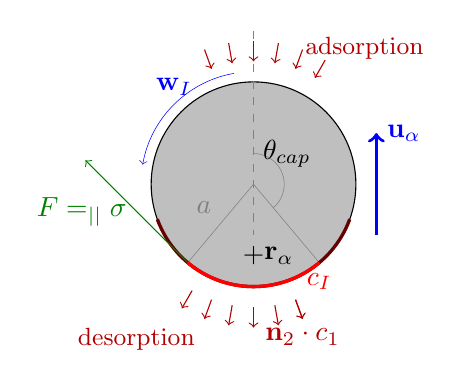
\begin{tikzpicture}[scale =1.3]
        \draw[fill=lightgray](0,0) circle (1);
        \draw[very thin,gray](230:1)--(0,0)node[midway,above left]{$a$}--(310:1);
        \draw[very thin,gray](0,0)++(310:0.3) arc (-50:90:0.3)node[right,black]{$\theta_\text{cap}$};
        \draw[very thin,blue,->](0,0)++(100:1.1) arc (100:170:1.1)node[midway,above]{$\textbf{w}_I$};
        \draw[very thick,red!40!black](0,0)++(200:1) arc (200:340:1);
        \draw[very thick,red](0,0)++(230:1) arc (230:310:1)node[below]{$c_I$};
        \draw[very thick,dashed](0,0)++(0,-0.7)node{$+$}node[right]{$\textbf{r}_\alpha$};
        \draw[very thick,blue,->](1.2,-0.5)--++(0,1)node[right]{$\textbf{u}_\alpha$};
        \draw[dashed,gray](0,1.5)--++(0,-2);
        \draw[red,->,green!50!black](230:1)--++(-1,1)node[midway,left]{$F = \grad_{||} \sigma$};
        \foreach \t in {110,100,90,80,60}{
            \draw[red!70!black, ->](\t:1.4)--++(\t:-0.2);
            \draw[red!70!black, ->](\t:-1.2)--++(\t:-0.2);
        }
        \draw[red!70!black, ->](70:1.4)--++(70:-0.2)node[above right]{\small adsorption};
        \draw[red!70!black, ->](70:-1.2)--++(70:-0.2)node[below left]{\small desorption};
        \draw[red!70!black, ->](110:-1.2)--++(110:-0.2)node[below]{$\textbf{n}_2 \cdot \grad c_1$};
    \end{tikzpicture}
    \hspace{2em}
    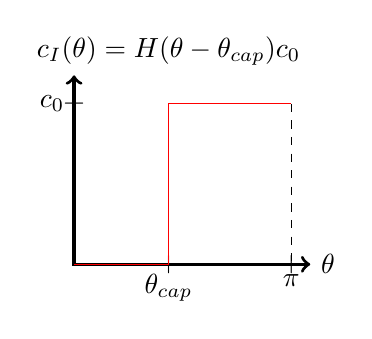
\begin{tikzpicture}[scale =1.2]
        \draw[very thick,<->](0,2)--(0,0)--(2.5,0)node[right]{$\theta$};
        \draw(1,0)node{$+$}node[below]{$\theta_{cap}$};
        \draw(1,2)node[above]{$c_I(\theta) = H(\theta- \theta_{cap}) c_0$};
        \draw[very thin,dashed](2.3,1.7)--(2.3,0);
        \draw[thin,red](0,0)--++(1,0)--++(0,1.7)--++(1.3,0);
        \draw(2.3,0)node{$+$}node[below]{$\pi$};
        \draw(0,1.7)node{$+$}node[left]{$c_0$};
    \end{tikzpicture}
    \caption{ (left) Scheme of the stagnant-cap regime of a rising contaminated bubble in a quiescent liquid. 
    (right) Hypothetical profile of the surface concentration $c_I$ in terms of the azimuthal coordinate $\theta$. }
    \label{fig:contaminated_bubbles}
\end{figure}


To derive the microscopic scale conservation equation of $c_I$ and $c_1$ we set $f_1 = c_1$ and $f_I = c_I$ in \ref{eq:dt_f_k} and \ref{eq:dt_f_I}, respectively.
Additionally, we assume that the  diffusive flux follow a Fick's law model, i.e.  $\mathbf{\Phi}_1 = D\grad c_1$ and $\mathbf{\Phi}_I = D_I\gradI c_I$,
where the constant,  $D$ and $D_I$ are the volumetric and surface diffusion coefficient, respectively.
Note that this diffusive model remains true under the assumption of dilute species concentration in both the liquid and at the interface.
\tb{The diffusive terms change in function of the regime : dilute concentration / saturated concentration, in which case $D\grad c_1 = f(c_I)$, it is worth going into that mush details ? no.}
Moreoverer, We do not consider chemical reaction or any other source term, i.e. $\textbf{S}_k = 0$ and $\textbf{S}_I=0$. 
Then, by injecting these terms in \ref{eq:dt_f_k} and \ref{eq:dt_f_I} we obtain these conservation equations : 
\begin{align}
    \pddt c_1
    + \div (\textbf{u}_1 c_1)
    &= \div (D \grad c_1)
    \;\;\; \text{in} \;\;\; \Omega_1,\\
    \pddt c_I
    + \divI (\textbf{u}_I c_I)
    &= \divI (D_I \gradI c_I)
    - (D \grad c_1)\cdot \textbf{n}_2
    \;\;\; \text{on} \;\;\; \Sigma,
    \label{eq:dt_c_I}
\end{align}
In agreement with \citet{pesci2018computational,manikantan2020surfactant}.
We recognize that the last term of \ref{eq:dt_c_I}, namely $D(\grad c_1 ) \cdot \textbf{n}_2$, turns out to be the \textit{Kinetically controlled sorption} boundary condition \citet{pesci2018computational,manikantan2020surfactant} which arise naturally in our model.
Specifically, it represents the adsorption and desorption flux between the bulk and the surface, as represented in \ref{fig:contaminated_bubbles}.
% For clarity remark that for exemple Equation (3.9) of \citet{manikantan2020surfactant} corresponds to the \textit{two-fluid} formulation of \ref{eq:dt_c_I} with a Fick's law model. 
Notice that this exchange term is reduced to a contribution from the continuous phase since we assume no surfactant into the dispersed phase. 
Now that we clearly derived the microscale equation in both phases, we can easily derive the averaged equations of conservation using the hybrid model presented \ref{sec:averaged_eq}.

For a better understanding of the following equations, we now describe the steady-state kinetics that can be reached for an isolated bubble in a contaminated flow, as illustrated on \ref{fig:contaminated_bubbles}.
This will serve as a reference for the subsequent discussion.
We first assume that the transport of surfactants on the surface, represented  by the term  $\textbf{w}_I c_I$, is much greater than the other diffusive processes, such as $D\grad c_1$ and $D_I\gradI c_I$ as well as the adsorption-desorption effects. 
In this regime, the concentration of surfactant that enters from the forward-surface, due to adsorption, is advected almost instantaneously to the downward region of the particle where some of it evaporates due to desorption. 
This form an accumulation of surfactant on the downward region of the particle's surface.
At a certain point of equilibrium, the adsorption and desorption flux balance each other, leading to the steady-state kinetic of $c_I$, and the stagnant cap is stabilized to a concentration $c_0$. 
In this situation, we can consider that $c_I$ follows a constant sharp distribution along the azimuthal coordinate of the particle's surface.
Specifically, we model $c_I(\theta) = H(\theta - \theta_{cap}) c_0$ where $H$ is the Heaviside function and $\theta_{cap}$ is the angle at which the stagnant cap is formed, see \ref{fig:contaminated_bubbles}.
This assumption might seem unrealistic, nevertheless in the steady-state regime, it is approximately consistent with the observations \citep{kentheswaran2022direct}.
% In these condition the physical meaning of the first moment, $\textbf{r}_\alpha$, becomes clearer. 
From the expression of $c_I$ we deduce : $C_\alpha = \frac{c_0}{2}(1+\cos\theta_{cap})$ and $\textbf{r}_\alpha = \frac{a}{2} (\cos\theta_{cap} -1)\textbf{e}$ where $\textbf{e}$ is the unit vector in the direction of the relative velocity between the particle and the continuous phase velocity.
Thus, the knowing $\textbf{r}_\alpha$ can leads use to $\theta_{cap}$. 
This is crucial information, since the drag forces term and mass transfer closure terms are usually derived in terms of $\theta_{cap}$, such as in the following studies : \citet{sadhal1983stokes} and \citet{kentheswaran2022direct}. 

Now that the problem has been properly formulated, we can begin the derivation of the averaged equations.
The phase-averaged conservation equation for the mean concentration of surfactant in the bulk $\oneavg{c}$, is derived using \ref{eq:avg_dt_chi_f}.
It reads as,
\begin{equation}
    \pddt (\phi_1 \oneavg{c})
    + \div (\phi_1 \oneavg{c} \oneavg{\textbf{u}_1})
    = D \grad^2 (\phi_1\oneavg{c})
    - \pnavg{j_\alpha}
    +  \div \mathbf{\Sigma}_c,
    \label{eq:hybrid_avg_dt_c_1}
\end{equation}
where $j_\alpha$ is the exchange term with the dispersed phase given by,
\begin{equation*}
    j_\alpha
    =\int_{\Sigma_\alpha}
    (D\grad c_1 )
\cdot \textbf{n}_2d\Sigma,
\end{equation*}
which corresponds to the resultant of the surfactant exchange including adsorption and desorption flux.  
In the steady-state regime, when the adsorption flux balance the desorption flux,  the surfactant on the surface of the bubble can be considered as globally insoluble since $j_\alpha=0$ even through $D(\grad c_1 ) \cdot \textbf{n}_2$ may not be locally zero. 
This \textit{globally insoluble} assumption has been used in numerous studies to neglect the adsorption-desorption fluxes. 
The vector $\mathbf{\Sigma}_c$ in \ref{eq:hybrid_avg_dt_c_1}, has the following expression,
\begin{equation}
    \mathbf{\Sigma}_c
    =
     \pnavg{\textbf{J}_\alpha}
    - \pnavg{\frac{D}{a}\int_{\Sigma_\alpha}  c_1 \textbf{r} d\Sigma}
    - \phi_1\oneavg{c'_1\textbf{u}_1'},
    \label{eq:B_def}
\end{equation}
where the higher order terms have been neglected. 
The first term on the RHS of \ref{eq:B_def} corresponds to the first moment of the surfactant flux, namely $\textbf{J}_\alpha = \int_{\Sigma_\alpha} \textbf{r}
(D\grad c_1)\cdot \textbf{n}_2d\Sigma$.
It can be interpreted as the vector representing the mean direction and magnitude of the surfactant flux going in and out the surface of the droplets.
In the stagnant cap regime, this term is therefore non-zero since a mean flux is still present even through its resultant is null, i.e. $j_\alpha=0$.
In the reference frame of the particles, $\textbf{J}_\alpha$ account for the mean flux of species concentration induced by the presence of the particles, due to adsorption and desorption phenomena. 
The second term of \ref{eq:B_def} comes from the inclusion of $\phi_1$ inside the Laplacian operator in \ref{eq:hybrid_avg_dt_c_1}.
It is the first moment of $c_1$ over the droplets surface, thus it is the mean position of the continuous phase surfactant concentration over the droplet surface.
For a constant distribution $c_1$ at the bubbles interface, this vector would be zero. 
Finally, The last term of \ref{eq:B_def}, $\phi_1\oneavg{c'_1\textbf{u}_1'}$, represents the diffusive term due to the correlation of $c'_1$ with $\textbf{u}_1'$.
Overall, $\mathbf{\Sigma}_c$ is a balance between the first moment of the fluxes and the first moment of the bulk concentration, minus a contribution from the fluctuations.
Notice that $\mathbf{\Sigma}_c$ appear under the divergence operator in \ref{eq:hybrid_avg_dt_c_1}, thus it will be relevant only in highly inhomogeneous cases. 
% At this stage of the research it is hard to predict the form of these closure terms. 
% Nevertheless, we know that the closure for $j_\alpha$ and $\mathbf{\Sigma}_c$ are function of the mean surface concentration $C_\alpha$ and its center of distribution $\textbf{r}_\alpha$.
% Indeed, the exchange term $\grad c_1$ which is function of the local concentration $c_I$ at surfactant saturation \citep{manikantan2020surfactant}. 
% Thus, an equation for $C_\alpha$ and a moment equation for $\textbf{r}_\alpha$ are needed. 

Regarding the equations dispersed phase, we start by the transport equation of the mean surface surfactant concentration $C_\alpha$.
From \ref{eq:avg_dt_dq_alpha_tot} the averaged conservation equation of $C_\alpha$ is straightforward to obtain and reads as,
\begin{equation}
    \pddt (\pnavg{C_\alpha})
    + \div (\pnavg{\textbf{u}_\alpha} \pnnavg{C_\alpha})
    =
    \frac{\pnavg{j_\alpha}}{s_\alpha}
    - \div (\pnavg{\textbf{u}_\alpha' C'_\alpha}).
    \label{eq:avg_dt_dC_alpha}
\end{equation}
As shown by this equation, the evolution of the mean concentration of surfactant on the particles' surface is driven by the exchange term $j_\alpha$ and the fluctuation term $\pnnavg{\textbf{u}_\alpha' C_\alpha'}$. 
The latter term is the covariance between the velocity of the particles and their mean surfactant concentration. 
It is known that the rising velocity of a bubble is greatly correlated with its mean surfactant concentration \citet{kentheswaran2022direct} thus it might be of a certain importance. 
Again, this term is under the divergence operator it will be therefore important only in non-homogeneous cases. 
Anyhow, this term must be further investigated.

We now derive an equation for the mean position of the surfactant, $\pnnavg{\textbf{r}_\alpha}$.
This is done by deriving the equation of the first moment, $s_\alpha C_\alpha \textbf{r}_\alpha$ using \ref{eq:dt_Q_alpha_tot}. 
Then, we reformulate the equation using  the relation, $\ddt (s_\alpha C_\alpha \textbf{r}_\alpha) = s_\alpha C_\alpha\ddt \textbf{r}_\alpha+ s_\alpha \textbf{r}_\alpha\ddt C_\alpha $ and  $\ddt C_\alpha = j_\alpha$. 
Finally,  we apply the average process which leads us to~:
\begin{multline}
    \pddt (\pnavg{\textbf{r}_\alpha})
    + \div (\pnavg{\textbf{u}_\alpha}\pnnavg{\textbf{r}_\alpha})
    =
    - \div (\pnavg{\textbf{u}'_\alpha\textbf{r}'_c})\\
    + \frac{n_p}{s_\alpha}\pnnavg{
        \frac{1}{C_\alpha}\left[
            \int_{\Sigma_\alpha} 
            \left[
                c_I \textbf{w}_I
                - D_I (\gradI c_I)
            \right] d\Sigma
            +\textbf{J}_\alpha
            - \textbf{r}_\alpha j_\alpha
        \right]
    }.
    \label{eq:avg_dt_dr_alpha_tot}
\end{multline}
The diffusive term $\pnavg{\textbf{u}'_\alpha\textbf{r}'_c}$ which represents the flux generated by the correlation between the mean surfactant distribution on the particles' surface and the velocity of the particles. 
Again, this term might be relevant since, as mentioned previously, the rising velocity is highly dependent on $\theta_{cap}$.
Then, the first term on the second line is the contribution of the averaged surface advection of $c_I$ along the particles' surface. 
The second term accounts for the diffusion of surfactants over the droplet surface, which acts against the formation of a sharp distribution of surfactants.
However, the contribution of this term is likely negligible based on the values of the diffusive surface coefficient, as discussed in \citet{valkovska2000determination}.
The third term of the second line, is the exchange term $\textbf{J}_\alpha$ which clearly impacts $\textbf{r}_\alpha$.
Indeed, this term accounts for the inward adsorption of concentration and downward desorption fluxes of surfactant, creating a significant disequilibrium. 
The last term, $\textbf{r}_\alpha j_\alpha$, is the contribution from the accumulation of species adsorption and desorption on the particle surface during the process driven by the three previous terms, i.e. adsorption, advection, diffusion and desorption. 
We may recognize that the latter fourth terms are being responsible for the equilibrium or not of the cap angle. 
Indeed, when all these terms are balanced, the system reaches a steady-state equilibrium for the surfactant distribution.
It is evident that in the closure of \ref{eq:avg_dt_dr_alpha_tot} one can include all properties linked to the physics of the bubbles' surface, which in turn creates a model for the surfactant distribution at first order. 

\tb{Dans cette partie il faut encore que je lise la bibliography qui existe peut etre sur ces dernière equaiton pour voir i le tout est bien coherent}

% \tb{Start : in the SSR the stagnat can is funciton of Re anfd Ma}
% Let assume that the timescale to reach the steady-state kinetic regime is much shorter than the variation of $\oneavg{c}$ seen by the particles. 
% In this situation the advection flux compensate the diffusive flux and adsorption-desorption source terms for all particles at all times.
% This equilibrium can be written :
% \begin{equation}
%     \int_{\Sigma_\alpha} 
%         c_I \textbf{w}_I
%         d\Sigma
%         - \int_{\Sigma_\alpha} 
%         D_I (\gradI c_I)
%          d\Sigma
%         +\textbf{J}_\alpha
%         = 0 
%         % - \textbf{r}_\alpha j_\alpha
%         \label{eq:steady_state_kinetic_regime}
% \end{equation}
% Nevertheless, due to a change of environment, $\oneavg{c}$ can change slowy inducing a non-zero $j_\alpha$, after what the particles reache instantaneously another steady-state kinetic regime. 
% In this situations the mean position of the surfactant is fully determined with the local concentration $\oneavg{c}$ or the local source $j_n$.
% Using the hypothesis \ref{eq:steady_state_kinetic_regime} in \ref{eq:avg_dt_dr_alpha_tot} gives the quasy steady conservation equaiton of $\textbf{r}_c$ with :
% \begin{equation}
%     \pddt (\pnavg{\textbf{r}_\alpha})
%     + \div (\pnavg{\textbf{u}_\alpha}\pnnavg{\textbf{r}_\alpha})
%     =
%     - \frac{n_p}{s_\alpha}\pnnavg{
%          \frac{\textbf{r}_\alpha j_\alpha}{C_\alpha}
%     }
%     - \div (\pnavg{\textbf{u}'_\alpha\textbf{r}'_c})
% \end{equation}
% where $\textbf{r}_\alpha$ is solely function on the local flux on the a the diffusive fluctuation term. 


As the objective of this study is not to provide a fully closed system, we will conclude the discussion on this point.
In short, this new system of equations can be used to determine the macroscopic variables $\pnnavg{C_\alpha}$ and $\pnnavg{\textbf{r}_\alpha}$, which are crucial for the closure of drag force and mass transfer in the macroscopic models.
Unfortunately, at the current state of the art, it is still challenging to derive exact closure terms for these equations, even in simplified regimes. 
However, we provided a clear methodology to derive a hybrid model tailored to the problem at hand, using the examples of surfactant transport and fiber suspension. 


% \section{Brouillion}
\subsection*{Fluid formulation meaningful exchange terms}


Using the generic formulation \ref{eq:hybrid_avg_dt_chif} and the local expression of the mass, momentum and total energy expression, i.e. : \ref{eq:dt_rho},\ref{eq:dt_rhou_1} and \ref{eq:dt_rhoE_1} we easily find the averaged form of these equations as, 

\begin{align}
    \pddt (\phi_1 \rho_1)  
    + \div (
        \phi_1 \rho_1\textbf{u}_1
    )
    &= 
    0\\
    \pddt (\phi_1 \rho_1\textbf{u}_1)  
    + \div (
        \phi_1 \rho_1\textbf{u}_1\textbf{u}_1
        + \bm{\sigma}_1^\text{eq}
    )
    &= 
    \phi_1 \rho_1 \textbf{g} 
    -  \avg{\delta_I \bm{\sigma}_1^0 \cdot \textbf{n}_2}\\
    \pddt (\phi_1\rho_1E_1)  
    + \div (
        \phi_1\rho_1E_1\textbf{u}_1
        + \bm{q}_1^\text{eq}
        + \textbf{u}_1 \cdot \bm{\sigma}_1^\text{eq}
        % - \textbf{u}_1^0 \cdot \bm{\sigma}_1^0 
        % + \textbf{q}_1^0
        )
    &= 
    \phi_1 \rho_1\textbf{u}_1 \cdot \textbf{g} 
    - \avg{\delta_I (\textbf{u}_1^0 \cdot \bm{\sigma}_1^0 - \textbf{q}_1^0)\cdot \textbf{n}_2}
\end{align} 
where we have defined, 
\begin{align*}
    &\bm{\sigma}_1^\text{eq}
    = \phi_1 (
        \rho_1\kavg{\textbf{u}_1'\textbf{u}_1'}
        - \bm{\sigma}_1%- n_p \textbf{M}_p
         )  
    &\textbf{q}_1^\text{eq}
    =\textbf{q}_1^\text{e} +\textbf{q}_1^\text{k}  \\
    &\textbf{q}_1^\text{e}
    = \phi_1\rho_1 \kavg{\textbf{u}_1' e_1'} 
    + \phi_1\textbf{q}_1 
    &\textbf{q}_1^\text{k}
    = \phi_1\rho_1 \kavg{\textbf{u}_1' k_1} 
    - \phi_1\kavg{\textbf{u}_1' \cdot \bm{\sigma}_1^0}
\end{align*}
Note that the phase averaged energy equation can be further decompose following, 
\begin{align*}
    E_1 = e_1 + k_1 + u_1^2/2
    \label{eq:E_def}
\end{align*}
where $K_1$ is the pseudo-turbulent kinetic energy defined such as, $\phi_1 k_1 = \avg{\chi_1 (u_1')^2/2}$. 
The Macroscopic kinetic energy equation can be obtain by taking the dot product with $\textbf{u}_1$. 
\begin{align}
    \pddt (\phi_1 \rho_1u_1^2/2)  
    + \div (
        \phi_1 \rho_1\textbf{u}_1u_1^2/2
        + \textbf{u}_1 \cdot \bm{\sigma}_1^\text{eq}
    )
    &= 
     \bm{\sigma}_1^\text{eq} : \grad \textbf{u}_1
    + \phi_1 \rho_1 \textbf{u}_1\cdot \textbf{g} 
    -  \textbf{u}_1\cdot \avg{\delta_I \bm{\sigma}_1^0 \cdot \textbf{n}_2}\\
    \pddt (\phi_1\rho_1k_1)  
    + \div (
        \phi_1\rho_1k_1\textbf{u}_1
        + \textbf{q}_1^\text{k} 
        )
    &= 
    - \avg{\chi_1\bm{\sigma}_1^0 : \grad \textbf{u}_1^0}
    - \bm{\sigma}_1^\text{eq} : \grad \textbf{u}_1
    - \avg{\delta_I \textbf{u}_1' \cdot \bm{\sigma}_1^0 \cdot \textbf{n}_2}\\
    \pddt (\phi_1\rho_1e_1)  
    + \div (
        \phi_1 \rho_1e_1\textbf{u}_1
        +
        \textbf{q}_1^\text{e} 
        )
    &= 
    \avg{\chi_1\bm{\sigma}_1^0 : \grad \textbf{u}_1^0}
    + \avg{\delta_I \textbf{q}_1^0 \cdot \textbf{n}_2} 
\end{align}


Let's decompose the exchange term $\avg{\delta_I \textbf{u}^0_1 \cdot \bm{\sigma}_1^0 \cdot \textbf{n}_2}$.
The first step is to make appear the drag force term 
\begin{align*}
    \avg{\delta_I \textbf{u}^0_1 \cdot \bm{\sigma}_1^0 \cdot \textbf{n}_2}
    = 
    \avg{\delta_I \textbf{u}^0_2 \cdot \bm{\sigma}_1^0 \cdot \textbf{n}_2}
    =
    \textbf{u}_p \cdot  \avg{\delta_I \bm{\sigma}_1^0 \cdot \textbf{n}_2}
    % + \avg{\delta_I (\textbf{u}_\alpha - \textbf{u}_p) \cdot \bm{\sigma}_1^0 \cdot \textbf{n}_2}
    + \avg{\delta_I (\textbf{u}^0_2 - \textbf{u}_p) \cdot \bm{\sigma}_1^0 \cdot \textbf{n}_2}
\end{align*}
Maybe it is not the good way. In fact let first do that : 
\begin{align*}
    \avg{\delta_I \textbf{u}^0_1 \cdot \bm{\sigma}_1^0 \cdot \textbf{n}_2}
    =
    \pavg{ \intS{\textbf{u}^0_2 \cdot \bm{\sigma}_1^0 \cdot \textbf{n}_2}}
    - \div\pavg{ \intS{\textbf{r}\textbf{u}^0_2 \cdot \bm{\sigma}_1^0 \cdot \textbf{n}_2}}
\end{align*}
The first term can then be written as, 
\begin{align*}
    \pavg{ \intS{\textbf{u}^0_2 \cdot \bm{\sigma}_1^0 \cdot \textbf{n}_2}}
    = 
    \textbf{u}_p \cdot \pavg{\intS{\bm{\sigma}_1^0 \cdot \textbf{n}_2}}
    + \pavg{ \textbf{u}_\alpha' \cdot \intS{  \bm{\sigma}_1^0 \cdot \textbf{n}_2}}
    + \pavg{ \intS{\textbf{w}_2^0 \cdot \bm{\sigma}_1^0 \cdot \textbf{n}_2}}
\end{align*}
\begin{align*}
    \pavg{ \intS{\textbf{r}\textbf{u}^0_2 \cdot \bm{\sigma}_1^0 \cdot \textbf{n}_2}}
    = 
    \textbf{u}_p \cdot \pavg{\intS{ \textbf{r}\bm{\sigma}_1^0 \cdot \textbf{n}_2}}
    + \pavg{ \textbf{u}_\alpha' \cdot \intS{ \textbf{r} \bm{\sigma}_1^0 \cdot \textbf{n}_2}}
    + \pavg{ \intS{\textbf{r}\textbf{w}_2^0 \cdot \bm{\sigma}_1^0 \cdot \textbf{n}_2}}
\end{align*}
Here we have a proper decomposition into surface work etc.. 


Using this formulation we can say that, 
\begin{align}
    \label{eq:dt_avg_rho}
    &\pddt (\phi_1 \rho_1)  
    + \div (
        \phi_1 \rho_1\textbf{u}_1
    )
    = 
    0\\
    \label{eq:dt_avg_rhou_1}
    &\pddt (\phi_1 \rho_1\textbf{u}_1)  
    + \div (
        \phi_1 \rho_1\textbf{u}_1\textbf{u}_1
        + \bm{\sigma}_1^\text{eq}
    )
    = 
    \phi_1 \rho_1 \textbf{g} 
    - \pavg{\intS{\bm{\sigma}_1^0 \cdot \textbf{n}_2}}
    +\div  \pavg{\intS{\textbf{r}\bm{\sigma}_1^0 \cdot \textbf{n}_2}}
    \\
    \label{eq:dt_avg_rhoE_1}
    &\pddt (\phi_1\rho_1E_1)  
    + \div (
        \phi_1\rho_1E_1\textbf{u}_1
        + \bm{q}_1^\text{eq}
        + \textbf{u}_1 \cdot \bm{\sigma}_1^\text{eq}
        % - \textbf{u}_1^0 \cdot \bm{\sigma}_1^0 
        % + \textbf{q}_1^0
        )
    = 
    \phi_1 \rho_1\textbf{u}_1 \cdot \textbf{g} \\
    &- \textbf{u}_p \cdot \pavg{\intS{\bm{\sigma}_1^0 \cdot \textbf{n}_2}}
    - \pavg{ \textbf{u}_\alpha' \cdot \intS{  \bm{\sigma}_1^0 \cdot \textbf{n}_2}}
    - \pavg{ \intS{\textbf{w}_2^0 \cdot \bm{\sigma}_1^0 \cdot \textbf{n}_2}}
    + \pavg{\intS{\textbf{q}_1\cdot \textbf{n}_2}}
    % &\div [    
        % \textbf{u}_p \cdot \pavg{\intS{ \textbf{r}\bm{\sigma}_1^0 \cdot \textbf{n}_2}}
    % + \pavg{ \textbf{u}_\alpha' \cdot \intS{ \textbf{r} \bm{\sigma}_1^0 \cdot \textbf{n}_2}}
    % + \pavg{ \intS{\textbf{r}\textbf{w}_2^0 \cdot \bm{\sigma}_1^0 \cdot \textbf{n}_2}}
    % - \pavg{ \intS{\textbf{r}  \textbf{q}_1^0 \cdot \textbf{n}_2}}
    % ]
\end{align} 
where we have defined, 
\begin{align*}
    &\bm{\sigma}_1^\text{eq}
    = \phi_1 (
        \rho_1\kavg{\textbf{u}_1'\textbf{u}_1'}
        -\bm{\sigma}_1%- n_p \textbf{M}_p
        )  
        - \pavg{\intS{\textbf{r}\bm{\sigma}_1^0 \cdot \textbf{n}_2}}\\
    &\textbf{q}_1^\text{eq}
    =\textbf{q}_1^\text{e} +\textbf{q}_1^\text{k}  \\
    &\textbf{q}_1^\text{e}
    = \phi_1\rho_1 \kavg{\textbf{u}_1' e_1'} 
    + \phi_1\textbf{q}_1 
    +\pavg{\intS{\textbf{r}\textbf{q}_1^0 \cdot \textbf{n}_2}} 
    \\
    &\textbf{q}_1^\text{k}
    = \phi_1\rho_1 \kavg{\textbf{u}_1' k_1} 
    - \phi_1\kavg{\textbf{u}_1' \cdot \bm{\sigma}_1^0}
    + (\textbf{u}_1 - \textbf{u}_p)\cdot
    \pavg{\intS{\textbf{r}\bm{\sigma}_1^0 \cdot \textbf{n}_2}}
    \\
    &+ \pavg{ \textbf{u}_\alpha' \cdot \intS{ \textbf{r} \bm{\sigma}_1^0 \cdot \textbf{n}_2}}
    + \pavg{ \intS{\textbf{r}\textbf{w}_2^0 \cdot \bm{\sigma}_1^0 \cdot \textbf{n}_2}}
\end{align*}
Let's re derive the Secondary equations, firstly the kinetic energy equaitons, 
\begin{align*}
    \pddt (\phi_1 \rho_1u_1^2/2)  
    + \div (
        \phi_1 \rho_1\textbf{u}_1u_1^2/2
        + \textbf{u}_1 \cdot \bm{\sigma}_1^\text{eq}
    )
    &= 
     \bm{\sigma}_1^\text{eq} : \grad \textbf{u}_1
    + \phi_1 \rho_1 \textbf{u}_1\cdot \textbf{g} 
    -  \textbf{u}_1\cdot 
        \pavg{\intS{\bm{\sigma}_1^0 \cdot \textbf{n}_2}} 
        % - \div 
        % \pavg{\intS{\textbf{r}\bm{\sigma}_1^0 \cdot \textbf{n}_2}} 
        \\
    \pddt (\phi_1\rho_1k_1)  
    + \div (
        \phi_1\rho_1k_1\textbf{u}_1
        + \textbf{q}_1^\text{k} 
        )
    &= 
    - \avg{\chi_1\bm{\sigma}_1^0 : \grad \textbf{u}_1^0}
    - \bm{\sigma}_1^\text{eq} : \grad \textbf{u}_1\\
    &+ (\textbf{u}_1 - \textbf{u}_p)
    \cdot \pavg{\intS{\bm{\sigma}_1^0 \cdot \textbf{n}_2}}\\
    &- \pavg{ \textbf{u}_\alpha' \cdot \intS{  \bm{\sigma}_1^0 \cdot \textbf{n}_2}}
    - \pavg{ \intS{\textbf{w}_2^0 \cdot \bm{\sigma}_1^0 \cdot \textbf{n}_2}} 
    \\
    \pddt (\phi_1\rho_1e_1)  
    + \div (
        \phi_1 \rho_1e_1\textbf{u}_1
        +
        \textbf{q}_1^\text{e} 
        )
    &= 
    \avg{\chi_1\bm{\sigma}_1^0 : \grad \textbf{u}_1^0}
    + \pavg{\intS{\textbf{q}_1^0 \cdot \textbf{n}_2}} 
\end{align*}
The second equality here, gives in a homogeneous medium, 
\begin{equation*}
    0 =
    - \avg{\chi_1\bm{\sigma}_1^0 : \grad \textbf{u}_1^0}
    % - \bm{\sigma}_1^\text{eq} : \grad \textbf{u}_1
    + (\textbf{u}_1 - \textbf{u}_p)
    \cdot \pavg{\intS{\bm{\sigma}_1^0 \cdot \textbf{n}_2}}
    - \pavg{ \textbf{u}_\alpha' \cdot \intS{  \bm{\sigma}_1^0 \cdot \textbf{n}_2}}
    - \pavg{ \intS{\textbf{w}_2^0 \cdot \bm{\sigma}_1^0 \cdot \textbf{n}_2}} 
\end{equation*}
\subsection*{Particle formulation meaningful exchange terms}

For the dispersed phase we initially have :
\begin{align*}
    \pddt \left(n_p m_p\right)
    + \div \left(n_pm_p\textbf{u}_p
    \right)
    = 
    0\\
    \pddt \left(n_p m_p \textbf{u}_p\right)
    + \div \left(n_p
    m_p \textbf{u}_p \textbf{u}_p 
    + \bm{\sigma}_p^\text{eq}
    \right)
    = 
    n_p v_p \rho_2 \textbf{g}
    + n_p (\bm{\sigma}_1^0 \cdot \textbf{n}_2)_p^\Sigma,\\
    \pddt(m_p n_pE_p^\text{tot})
    + \div(m_pn_p E_p^\text{tot} \textbf{u}_p 
    + \textbf{q}_p^\text{eq} 
    + \textbf{u}_p \cdot \bm{\sigma}_p^\text{eq})
    =  n_p v_p \rho_2 \textbf{u}_p\cdot  \textbf{g}\\
    % +  n_p ( \textbf{u}'_1 \cdot \bm{\sigma}_1^0 \cdot \textbf{n}_2)_p^\Sigma
    -  n_p (\textbf{q}_1^0 \cdot \textbf{n}_2)_p^\Sigma
    + \textbf{u}_p \cdot\pavg{\intS{\bm{\sigma}_1^0 \cdot \textbf{n}_2}}
    + \pavg{\intS{\textbf{u}_\alpha' \cdot\bm{\sigma}_1^0 \cdot \textbf{n}_2}}
    + \pavg{\intS{\textbf{w}_2^0 \cdot\bm{\sigma}_1^0 \cdot \textbf{n}_2}}
\end{align*}
where we have defined, 
\begin{align*}
    &\bm{\sigma}_p^\text{eq}
    =  m_p\pnavg{\textbf{u}_\alpha'\textbf{u}_\alpha'}
    &\textbf{q}_p^\text{eq}
    =\textbf{q}_p^\text{e} 
    +\textbf{q}_p^\text{k}  
    +\textbf{q}_p^\text{w}  
    \\
    &\textbf{q}_1^\text{e}
    = m_p \pnavg{\textbf{u}_\alpha' e_\alpha'} 
    &\textbf{q}_p^\text{k}
    = m_p \pnavg{\textbf{u}_\alpha' k_\alpha} 
    \\
    &\textbf{q}_p^\text{w}
    = 
    + \pnavg{\textbf{u}_\alpha'(\rho_2 (w^0_2)^2/2 )'_\Omega}
    + \gamma \pnavg{\textbf{u}_\alpha' s_\alpha'}
\end{align*}
and, 
The exchange term of the energy equation can be rewritten as, 
\begin{equation*}
    \pavg{\intS{\textbf{u}_1^0\cdot\bm{\sigma}_1^0 \cdot \textbf{n}_2}}
    = 
    \textbf{u}_p \cdot\pavg{\intS{\bm{\sigma}_1^0 \cdot \textbf{n}_2}}
    + \pavg{\intS{\textbf{u}_\alpha' \cdot\bm{\sigma}_1^0 \cdot \textbf{n}_2}}
    + \pavg{\intS{\textbf{w}_2^0 \cdot\bm{\sigma}_1^0 \cdot \textbf{n}_2}}
\end{equation*}
Also, 
\begin{align*}
    &\pddt \left(n_p m_p u_p^2/ 2\right)
    + \div \left(n_p
    m_p u_p^2/ 2 \textbf{u}_p 
    + \textbf{u}_p \cdot \bm{\sigma}_p^\text{eq}
    \right)
    = 
    + \bm{\sigma}_p^\text{eq}  :\grad \textbf{u}_p
    +  n_p v_p \textbf{u}_p \cdot 
    \rho_2 \textbf{g}
    + n_p \textbf{u}_p \cdot (\bm{\sigma}_1^0 \cdot \textbf{n}_2)^\Sigma_p,\\
    &\pddt \left(n_p m_p (u_\alpha^2)_p/ 2\right)
    + \div \left(n_p
    m_p (u_\alpha^2)_p/ 2 \textbf{u}_p 
    + \textbf{q}^k_p
    + \textbf{u}_p \cdot \bm{\sigma}_p^\text{eq}
    \right)
    = 
    n_p m_p \textbf{u}_p \cdot
    \textbf{g}
    + \textbf{u}_p\cdot\pavg{\intS{\bm{\sigma}_1^0 \cdot \textbf{n}_2}}\\
    &+ \pavg{\textbf{u}_\alpha'\cdot\intS{\bm{\sigma}_1^0 \cdot \textbf{n}_2}}
    \\
    &\pddt \left(n_p W_p\right)
    + \div 
    (n_p W_p
    \textbf{u}_p 
    +  \textbf{q}_p^\text{w}
    )
    = 
    - n_p (\bm{\sigma}_2^0 : \grad\textbf{u}_2^0)^\Omega_p
    + n_p (\textbf{w}_2^0 \cdot \bm{\sigma}_1^0 \cdot  \textbf{n}_2)^\Sigma_p
    \\
    &\pddt \left(n_p m_p e_p\right)
    + \div \left(n_p
    m_p e_p \textbf{u}_p 
    +  \textbf{q}_p^\text{e}
    \right)
    = 
    + n_p (\bm{\sigma}_2^0 : \grad\textbf{u}_2^0)^\Omega_p
    - n_p (\textbf{q}_1^0\cdot \textbf{n}_2)^\Sigma_p\\
\end{align*}
The equaiton for $k_p$ reads, 
\begin{equation*}
    \pddt \left(n_p m_p k_p\right)
    + \div \left(n_p
    m_p k_p \textbf{u}_p 
    + \textbf{q}^k_p
    % + \textbf{u}_p \cdot \bm{\sigma}_p^\text{eq}
    \right)
    = 
    - \bm{\sigma}_p^\text{eq}  :\grad \textbf{u}_p
    + \pavg{\textbf{u}_\alpha'\cdot\intS{\bm{\sigma}_1^0 \cdot \textbf{n}_2}}
\end{equation*}
In agreement with kinetic theory without source term. 


Under this form the NRJ cascade takes the form
\begin{center}
    \tikzstyle{quadri}=[rectangle,draw]
    \begin{tikzpicture}
        \node[quadri] (u2) at (0,0){$(u_p)^2 / 2$};
        \node[quadri] (kp) at (4,0){$(k_p)$};
        \node[quadri] (Wp) at (8,0){$(W_p)$};
        \node[quadri] (ep) at (12,0){$(e_p)$};
        \node[quadri] (u12) at (2,-3){$\frac{\rho_1}{2}(u_1)^2$};
        \node[quadri] (k1) at (6,-3){$k_1$};
        \node[quadri] (e1) at (10,-3){$e_1$};
        \draw[->] (u2)--(kp)node[midway,above]{\footnotesize $\bm{\sigma}^\text{eq}:\grad \textbf{u}_1$};
        \draw[<->] (u2)--(u12) node[midway,left]{\footnotesize $\textbf{f}_{p} $};
        % \draw[<->,text width=2cm] (kp)--(u12) node[midway,left]{\footnotesize $+  n_p v_p \textbf{u}_p \cdot 
        % (\rho_2 \textbf{g} - \grad p_1)
        % + n_p \textbf{u}_p \cdot \textbf{f}_{pm} - \textbf{F}_\text{pfp}$};
        \draw[<->] (k1)--(u12) node[midway,below]{\footnotesize $\bm{\sigma}^\text{eq}_1:\grad \textbf{u}_1$, $\textbf{f}_p$};
        \draw[<->] (k1)--(e1) node[midway,below]{\footnotesize $\textbf{d}_1$};
        \draw[<->,sloped] (k1)--(kp) node[midway,below]{\footnotesize $\pavg{\textbf{f}_\alpha\cdot \textbf{u}_\alpha'}$};
        \draw[<->] (k1)--(u2) node[midway,below]{\footnotesize $\textbf{f}_p$};
        \draw[<->,sloped] (k1)--(Wp) node[midway,below]{\footnotesize $\pavg{\intS{\textbf{w}_2^0\cdot \textbf{f}_1^0}}$};
        % \draw[->] (kp)--(Wp)node[midway,above]{$(\textbf{u}_\alpha' \cdot \textbf{f}_\alpha')_p$};
        \draw[->] (Wp)--(ep)node[midway,above]{$\textbf{d}_p$};
        \draw[->] (e1)--(ep)node[midway,above]{$\textbf{q}_p$};
    \end{tikzpicture}
\end{center}

Thus, from this graph it is clear that the only way to makes the link between $k_p$ and the NRJ dissipation is through the addition of $k_p$ and $W_p$. Which gives, 
\begin{multline*}
    \pddt \left(n_p (W_p+m_p k_p)\right)
    + \div 
    (n_p (W_p+m_p k_p)
    \textbf{u}_p 
    +  \textbf{q}_p^\text{w}
    +  \textbf{q}_p^\text{k}
    )\\
    = 
    - n_p (\bm{\sigma}_2^0 : \grad\textbf{u}_2^0)^\Omega_p
    + n_p (\textbf{w}_2^0 \cdot \bm{\sigma}_1^0 \cdot  \textbf{n}_2)^\Sigma_p
    - \bm{\sigma}_p^\text{eq}  :\grad \textbf{u}_p
    + \pavg{\textbf{u}_\alpha'\cdot\intS{\bm{\sigma}_1^0 \cdot \textbf{n}_2}}
\end{multline*}
Here we recover the transfer terms of with the higher scales and the lower scales plus the ones of the fluid continuous phase...
In kinetic theory we consider non-slipping spherical particles such that the internal motion are constant, and non rotation is present.
In this situation it yields 
\begin{equation}
    \pddt \left(n_p m_p k_p\right)
    + \div 
    (n_p m_p k_p
    \textbf{u}_p 
    % +  \textbf{q}_p^\text{w}
    +  \textbf{q}_p^\text{k}
    )
    = 
    - n_p (\bm{\sigma}_2^0 : \grad\textbf{u}_2^0)^\Omega_p
    + n_p (\textbf{w}_2^0 \cdot \bm{\sigma}_1^0 \cdot  \textbf{n}_2)^\Sigma_p
    - \bm{\sigma}_p^\text{eq}  :\grad \textbf{u}_p
    + \pavg{\textbf{u}_\alpha'\cdot\intS{\bm{\sigma}_1^0 \cdot \textbf{n}_2}}
\end{equation}
Indeed, we still consider deformation inside the particles since a source term of dissipation is constant. 



\subsection{Inclusion of long range interactions}
\subsubsection*{Fluid phase}

Using this formulation we can say that, 
\begin{align}
    \label{eq:dt_avg_rho}
    &\pddt (\phi_1 \rho_1)  
    + \div (
        \phi_1 \rho_1\textbf{u}_1
    )
    = 
    0\\
    \label{eq:dt_avg_rhou_1}
    &\pddt (\phi_1 \rho_1\textbf{u}_1)  
    + \div (
        \phi_1 \rho_1\textbf{u}_1\textbf{u}_1
        + \bm{\sigma}_1^\text{eq}
    )
    = 
    \phi_1 \rho_1 \textbf{g} 
    % +  \pavg{\intS{\bm{\sigma}_1^0 \cdot \textbf{n}_2}}
    - n_p (\textbf{f}_\text{pm} + v_p \grad p_1)
    % +\div  \pavg{\intS{\textbf{r}\bm{\sigma}_1^0 \cdot \textbf{n}_2}}
    \\
    \label{eq:dt_avg_rhoE_1}
    &\pddt (\phi_1\rho_1E_1)  
    + \div (
        \phi_1\rho_1E_1\textbf{u}_1
        + \bm{q}_1^\text{eq}
        + \textbf{u}_1 \cdot \bm{\sigma}_1^\text{eq}
        % - \textbf{u}_1^0 \cdot \bm{\sigma}_1^0 
        % + \textbf{q}_1^0
        )
    = 
    \phi_1 \rho_1\textbf{u}_1 \cdot \textbf{g} 
    +n_p\textbf{F}_\text{pfp}:\grad \textbf{u}_p\\
    &
    - n_p \textbf{u}_p \cdot (\textbf{f}_\text{pm} + v_p \grad p_1)
    % \pavg{\intS{\bm{\sigma}_1^0 \cdot \textbf{n}_2}}
    - \pavg{ \textbf{u}_\alpha' \cdot \intS{  \bm{\sigma}_1^0 \cdot \textbf{n}_2}}
    - \pavg{ \intS{\textbf{w}_2^0 \cdot \bm{\sigma}_1^0 \cdot \textbf{n}_2}}
    + \pavg{\intS{\textbf{q}_1\cdot \textbf{n}_2}}
    % &\div [    
        % \textbf{u}_p \cdot \pavg{\intS{ \textbf{r}\bm{\sigma}_1^0 \cdot \textbf{n}_2}}
    % + \pavg{ \textbf{u}_\alpha' \cdot \intS{ \textbf{r} \bm{\sigma}_1^0 \cdot \textbf{n}_2}}
    % + \pavg{ \intS{\textbf{r}\textbf{w}_2^0 \cdot \bm{\sigma}_1^0 \cdot \textbf{n}_2}}
    % - \pavg{ \intS{\textbf{r}  \textbf{q}_1^0 \cdot \textbf{n}_2}}
    % ]
\end{align} 
where we have defined, 
\begin{align*}
    &\bm{\sigma}_1^\text{eq}
    = \phi_1 (
        \rho_1\kavg{\textbf{u}_1'\textbf{u}_1'}
        -\bm{\sigma}_1%- n_p \textbf{M}_p
        )  
        - \pavg{\intS{\textbf{r}\bm{\sigma}_1^0 \cdot \textbf{n}_2}}
        + \textbf{F}_\text{pfp}\\
    &\textbf{q}_1^\text{eq}
    =\textbf{q}_1^\text{e} +\textbf{q}_1^\text{k}  \\
    &\textbf{q}_1^\text{e}
    = \phi_1\rho_1 \kavg{\textbf{u}_1' e_1'} 
    + \phi_1\textbf{q}_1 
    +\pavg{\intS{\textbf{r}\textbf{q}_1^0 \cdot \textbf{n}_2}} 
    \\
    &\textbf{q}_1^\text{k}
    = \phi_1\rho_1 \kavg{\textbf{u}_1' k_1} 
    - \phi_1\kavg{\textbf{u}_1' \cdot \bm{\sigma}_1^0}
    + (\textbf{u}_1 - \textbf{u}_p)\cdot[
    \pavg{\intS{\textbf{r}\bm{\sigma}_1^0 \cdot \textbf{n}_2}}
     - n_p \textbf{F}_\text{pfp}]
    \\
    &+ \pavg{ \textbf{u}_\alpha' \cdot \intS{ \textbf{r} \bm{\sigma}_1^0 \cdot \textbf{n}_2}}
    + \pavg{ \intS{\textbf{r}\textbf{w}_2^0 \cdot \bm{\sigma}_1^0 \cdot \textbf{n}_2}}
\end{align*}
Let's re derive the Secondary equations, firstly the kinetic energy equaitons, 
\begin{align*}
    \pddt (\phi_1 \rho_1u_1^2/2)  
    + \div (
        \phi_1 \rho_1\textbf{u}_1u_1^2/2
        + \textbf{u}_1 \cdot \bm{\sigma}_1^\text{eq}
    )
    &= 
     \bm{\sigma}_1^\text{eq} : \grad \textbf{u}_1
    + \phi_1 \rho_1 \textbf{u}_1\cdot \textbf{g} 
    -  n_p \textbf{u}_1\cdot 
    (\textbf{f}_\text{pm} + v_1\grad p_1)
        % \pavg{\intS{\bm{\sigma}_1^0 \cdot \textbf{n}_2}} 
        % - \div 
        % \pavg{\intS{\textbf{r}\bm{\sigma}_1^0 \cdot \textbf{n}_2}} 
        \\
    \pddt (\phi_1\rho_1k_1)  
    + \div (
        \phi_1\rho_1k_1\textbf{u}_1
        + \textbf{q}_1^\text{k} 
        )
    &= 
    - \avg{\chi_1\bm{\sigma}_1^0 : \grad \textbf{u}_1^0}
    - \bm{\sigma}_1^\text{eq} : \grad \textbf{u}_1
    + n_p \textbf{F}_\text{pfp} : \grad \textbf{u}_p
    \\
    &+ n_p (\textbf{u}_1 - \textbf{u}_p)
    \cdot (\textbf{f}_\text{pm} - v_p \grad p_1)\\
    &- \pavg{ \textbf{u}_\alpha' \cdot \intS{  \bm{\sigma}_1^0 \cdot \textbf{n}_2}}
    - \pavg{ \intS{\textbf{w}_2^0 \cdot \bm{\sigma}_1^0 \cdot \textbf{n}_2}} 
    \\
    \pddt (\phi_1\rho_1e_1)  
    + \div (
        \phi_1 \rho_1e_1\textbf{u}_1
        +
        \textbf{q}_1^\text{e} 
        )
    &= 
    \avg{\chi_1\bm{\sigma}_1^0 : \grad \textbf{u}_1^0}
    + \pavg{\intS{\textbf{q}_1^0 \cdot \textbf{n}_2}} 
\end{align*}
The homogeneous equilibrium stays the same. 
\subsection*{Particle phase with pfp and dumped pressure}
On the particle phase


For the dispersed phase we initially have :
\begin{align*}
    \pddt \left(n_p m_p\right)
    + \div \left(n_pm_p\textbf{u}_p
    \right)
    = 
    0\\
    \pddt \left(n_p m_p \textbf{u}_p\right)
    + \div \left(n_p
    m_p \textbf{u}_p \textbf{u}_p 
    + \bm{\sigma}_p^\text{eq}
    \right)
    = 
    n_p v_p \rho_2 \textbf{g}
    + n_p (\textbf{f}_\text{pm} + v_p \grad p_1),
    \\
    \pddt(m_p n_pE_p^\text{tot})
    + \div(m_pn_p E_p^\text{tot} \textbf{u}_p 
    + \textbf{q}_p^\text{eq} 
    + \textbf{u}_p \cdot \bm{\sigma}_p^\text{eq})
    =  n_p v_p \rho_2 \textbf{u}_p\cdot  \textbf{g}
    % +  n_p ( \textbf{u}'_1 \cdot \bm{\sigma}_1^0 \cdot \textbf{n}_2)_p^\Sigma
    -  n_p (\textbf{q}_1^0 \cdot \textbf{n}_2)_p^\Sigma\\
    - n_p \textbf{F}_\text{pfp} : \grad \textbf{u}_p
    + \textbf{u}_p \cdot (\textbf{f}_\text{pm} + v_p\grad p_1)
    + \pavg{\intS{\textbf{u}_\alpha' \cdot\bm{\sigma}_1^0 \cdot \textbf{n}_2}}
    + \pavg{\intS{\textbf{w}_2^0 \cdot\bm{\sigma}_1^0 \cdot \textbf{n}_2}}
\end{align*}
where we have defined, 
\begin{align*}
    &\bm{\sigma}_p^\text{eq}
    =  m_p\pnavg{\textbf{u}_\alpha'\textbf{u}_\alpha'}
    - n_p \textbf{F}_\text{pfp}
    &\textbf{q}_p^\text{eq}
    =\textbf{q}_p^\text{e} 
    +\textbf{q}_p^\text{k}  
    +\textbf{q}_p^\text{w}  
    \\
    &\textbf{q}_1^\text{e}
    = m_p \pnavg{\textbf{u}_\alpha' e_\alpha'} 
    &\textbf{q}_p^\text{k}
    = m_p \pnavg{\textbf{u}_\alpha' k_\alpha} 
    \\
    &\textbf{q}_p^\text{w}
    = 
    + \pnavg{\textbf{u}_\alpha'(\rho_2 (w^0_2)^2/2 )'_\Omega}
    + \gamma \pnavg{\textbf{u}_\alpha' s_\alpha'}
\end{align*}
Also, 
\begin{align*}
    &\pddt \left(n_p m_p u_p^2/ 2\right)
    + \div \left(n_p
    m_p u_p^2/ 2 \textbf{u}_p 
    + \textbf{u}_p \cdot \bm{\sigma}_p^\text{eq}
    \right)
    = 
    + \bm{\sigma}_p^\text{eq}  :\grad \textbf{u}_p
    +  n_p v_p \textbf{u}_p \cdot 
    \rho_2 \textbf{g}
    + n_p \textbf{u}_p \cdot (\textbf{f}_\text{pm} + v_p \grad p_1),\\
    &\pddt \left(n_p m_p (u_\alpha^2)_p/ 2\right)
    + \div \left(n_p
    m_p (u_\alpha^2)_p/ 2 \textbf{u}_p 
    + \textbf{q}^k_p
    + \textbf{u}_p \cdot \bm{\sigma}_p^\text{eq}
    \right)
    = 
    n_p m_p \textbf{u}_p \cdot
    \textbf{g}
    + \textbf{u}_p\cdot(\textbf{f}_\text{pm} + v_p \grad p_1)\\
    &- n_p \textbf{F}_\text{pfp} : \grad \textbf{u}_p
    + \pavg{\textbf{u}_\alpha'\cdot\intS{\bm{\sigma}_1^0 \cdot \textbf{n}_2}}
    \\
    &\pddt \left(n_p W_p\right)
    + \div 
    (n_p W_p
    \textbf{u}_p 
    +  \textbf{q}_p^\text{w}
    )
    = 
    - n_p (\bm{\sigma}_2^0 : \grad\textbf{u}_2^0)^\Omega_p
    + n_p (\textbf{w}_2^0 \cdot \bm{\sigma}_1^0 \cdot  \textbf{n}_2)^\Sigma_p
    \\
    &\pddt \left(n_p m_p e_p\right)
    + \div \left(n_p
    m_p e_p \textbf{u}_p 
    +  \textbf{q}_p^\text{e}
    \right)
    = 
    + n_p (\bm{\sigma}_2^0 : \grad\textbf{u}_2^0)^\Omega_p
    - n_p (\textbf{q}_1^0\cdot \textbf{n}_2)^\Sigma_p\\
\end{align*}
The equaiton for $k_p$ reads, 
\begin{equation*}
    \pddt \left(n_p m_p k_p\right)
    + \div \left(n_p
    m_p k_p \textbf{u}_p 
    + \textbf{q}^k_p
    % + \textbf{u}_p \cdot \bm{\sigma}_p^\text{eq}
    \right)
    = 
    - \pavg{\textbf{u}_\alpha'\textbf{u}_\alpha'} :\grad \textbf{u}_p
    + \pavg{\textbf{u}_\alpha'\cdot\intS{\bm{\sigma}_1^0 \cdot \textbf{n}_2}}
\end{equation*}
In agreement with kinetic theory without source term. 


Under this form the NRJ cascade takes the form
\begin{center}
    \tikzstyle{quadri}=[rectangle,draw]
    \begin{tikzpicture}
        \node[quadri] (u2) at (0,0){$(u_p)^2 / 2$};
        \node[quadri] (kp) at (4,0){$(k_p)$};
        \node[quadri] (Wp) at (8,0){$(W_p)$};
        \node[quadri] (ep) at (12,0){$(e_p)$};
        \node[quadri] (u12) at (2,-3){$\frac{\rho_1}{2}(u_1)^2$};
        \node[quadri] (k1) at (6,-3){$k_1$};
        \node[quadri] (e1) at (10,-3){$e_1$};
        \draw[->] (u2)--(kp)node[midway,above]{\footnotesize $\bm{\sigma}^\text{eq}:\grad \textbf{u}_1$};
        \draw[<->] (u2)--(u12) node[midway,left]{\footnotesize $\textbf{f}_{p} $};
        % \draw[<->,text width=2cm] (kp)--(u12) node[midway,left]{\footnotesize $+  n_p v_p \textbf{u}_p \cdot 
        % (\rho_2 \textbf{g} - \grad p_1)
        % + n_p \textbf{u}_p \cdot \textbf{f}_{pm} - \textbf{F}_\text{pfp}$};
        \draw[<->] (k1)--(u12) node[midway,below]{\footnotesize $\bm{\sigma}^\text{eq}_1:\grad \textbf{u}_1$, $\textbf{f}_p$};
        \draw[<->] (k1)--(e1) node[midway,below]{\footnotesize $\textbf{d}_1$};
        \draw[<->,sloped] (k1)--(kp) node[midway,below]{\footnotesize $\pavg{\textbf{f}_\alpha\cdot \textbf{u}_\alpha'}$};
        \draw[<->] (k1)--(u2) node[midway,below]{\footnotesize $\textbf{f}_p$};
        \draw[<->,sloped] (k1)--(Wp) node[midway,below]{\footnotesize $\pavg{\intS{\textbf{w}_2^0\cdot \textbf{f}_1^0}}$};
        % \draw[->] (kp)--(Wp)node[midway,above]{$(\textbf{u}_\alpha' \cdot \textbf{f}_\alpha')_p$};
        \draw[->] (Wp)--(ep)node[midway,above]{$\textbf{d}_p$};
        \draw[->] (e1)--(ep)node[midway,above]{$\textbf{q}_p$};
    \end{tikzpicture}
\end{center}

Thus, from this graph it is clear that the only way to makes the link between $k_p$ and the NRJ dissipation is through the addition of $k_p$ and $W_p$. Which gives, 
\begin{multline*}
    \pddt \left(n_p (W_p+m_p k_p)\right)
    + \div 
    (n_p (W_p+m_p k_p)
    \textbf{u}_p 
    +  \textbf{q}_p^\text{w}
    +  \textbf{q}_p^\text{k}
    )\\
    = 
    - n_p (\bm{\sigma}_2^0 : \grad\textbf{u}_2^0)^\Omega_p
    + n_p (\textbf{w}_2^0 \cdot \bm{\sigma}_1^0 \cdot  \textbf{n}_2)^\Sigma_p
    - \bm{\sigma}_p^\text{eq}  :\grad \textbf{u}_p
    + \pavg{\textbf{u}_\alpha'\cdot\intS{\bm{\sigma}_1^0 \cdot \textbf{n}_2}}
\end{multline*}
Here we recover the transfer terms of with the higher scales and the lower scales plus the ones of the fluid continuous phase...
In kinetic theory we consider non-slipping spherical particles such that the internal motion are constant, and non rotation is present.
In this situation it yields 
\begin{equation}
    \pddt \left(n_p m_p k_p\right)
    + \div 
    (n_p m_p k_p
    \textbf{u}_p 
    % +  \textbf{q}_p^\text{w}
    +  \textbf{q}_p^\text{k}
    )
    = 
    - n_p (\bm{\sigma}_2^0 : \grad\textbf{u}_2^0)^\Omega_p
    + n_p (\textbf{w}_2^0 \cdot \bm{\sigma}_1^0 \cdot  \textbf{n}_2)^\Sigma_p
    - \bm{\sigma}_p^\text{eq}  :\grad \textbf{u}_p
    + \pavg{\textbf{u}_\alpha'\cdot\intS{\bm{\sigma}_1^0 \cdot \textbf{n}_2}}
\end{equation}
Indeed, we still consider deformation inside the particles since a source term of dissipation is constant. 


% \Huge{ \tb{Brouillion}}\normalsize


\section{The ultimate model ?}
The main idea is to let the internal viscous term of particles : $\lambda \phi_2 \bm{\tau}_2$ within the divergence of the momentum equation to recover the proper Stresslet term, i.e $\mathscr{S}_p = n_p(\textbf{r} \bm{\sigma}_1^0 \cdot \textbf{n})_p^\Sigma -n_p(\textbf{r} \cdot \bm{\sigma}_1^0 \cdot \textbf{n})_p^\Sigma \textbf{I} - \lambda \phi_2 \bm{\tau}_2$. 
The trace of the stress let might be removed by the use of the averaged pressure $p_1$ present in the models below. 
How about the viscosity ratio part ? Well it can be show that, 
\begin{align*}
    n_p (\textbf{r} \bm{\sigma}_1'\cdot \textbf{n}_1)_p^\Sigma
    = 
    n_p (\textbf{r} \bm{\sigma}_1^0\cdot \textbf{n}_1)_p^\Sigma
    - n_p v_p \bm{\sigma}_1 
\end{align*}
From the formulas, 
\begin{align*}
    \bm{\sigma}_1 \phi_1
    &=- \phi_1 p_1 \textbf{I}
    + \mu_1 \textbf{e}
    - \lambda \phi_2 \bm{\tau}_2\\
    \bm{\sigma}_1 n_p v_p 
    &=- n_p v_p p_1 \textbf{I}
    + \frac{n_p v_p}{\phi_1}\mu_1 \textbf{e}
    - \lambda \frac{n_pv_p\phi_2}{\phi_1} \bm{\tau}_2
\end{align*}
we see that we hardly recover the real stresslet, because under this form the term related to the particle shear is lumped into the divergence at the other side of the equations. 
Therefore, the BEST model is the one were we throw $-p_1$ and $\textbf{q}_1$ on the Others side of the  equaiton. 
Note that the trace of $n_p(\textbf{r} \cdot (\bm{\sigma}_1^0 - p_1) \cdot \textbf{n})_p^\Sigma \textbf{I}$ is surely null since no pressure force form the normal viscous force is possible. 

In a shearing problem this might be not the best option because the mean shear isn't subtracted to the drag and first moment. 

\subsection*{Fluid phase}

Using the generic formulation \ref{eq:hybrid_avg_dt_chif} and the local expression of the mass, momentum and total energy expression, i.e. : \ref{eq:dt_rho},\ref{eq:dt_rhou_k} and \ref{eq:dt_rhoE_k} we easily find the averaged form of these equations as, 
\begin{align}
    \label{eq:dt_&vg_rho}
    \pddt (\phi_1 \rho_1)  
    + \div (
        \phi_1 \rho_1\textbf{u}_1
    )
    &= 
    0\\
    \label{eq:dt_&vg_rhou_1}
    \pddt (\phi_1 \rho_1\textbf{u}_1)  
    + \div (
        \phi_1 \rho_1\textbf{u}_1\textbf{u}_1
        + \bm{\sigma}_1^\text{eq}
    )
    &= 
    \phi_1 (\rho_1 \textbf{g} 
    - \grad p_1 ) 
    -  \avg{\delta_I \bm{\sigma}_1' \cdot \textbf{n}_2}\\
    \label{eq:dt_&vg_rhoE_1}
    \pddt (\phi_1\rho_1E_1)  
    + \div (
        \phi_1\rho_1E_1\textbf{u}_1
        + \bm{q}_1^\text{eq}
        + \textbf{u}_1 \cdot \bm{\sigma}_1^\text{eq}
        % - \textbf{u}_1^0 \cdot \bm{\sigma}_1^0 
        % + \textbf{q}_1^0
        )
    &= 
    \phi_1 [\rho_1\textbf{u}_1 \cdot \textbf{g} 
    - \div(\textbf{u}_1p_1 + \textbf{q}_1)]
    - \textbf{u}_1 \cdot\avg{\delta_I \bm{\sigma}_1'\cdot \textbf{n}_2}\nonumber\\
    &- \avg{\delta_I (\textbf{u}_1' \cdot \bm{\sigma}_1^0 )\cdot \textbf{n}_2}
    + \avg{\delta_I\textbf{q}_1'\cdot \textbf{n}_2}
\end{align} 
\begin{align*}
    &\bm{\sigma}_1^\text{eq}
    = \phi_1\rho_1\kavg{\textbf{u}_1'\textbf{u}_1'}
    - \bm{\tau}_1 \phi_1
    &\textbf{q}_1^\text{eq}
    =\textbf{q}_1^\text{e} +\textbf{q}_1^\text{k}  \\
    &\textbf{q}_1^\text{e}
    = \phi_1\rho_1 \kavg{\textbf{u}_1' e_1'} 
    &\textbf{q}_1^\text{k}
    = \phi_1\rho_1 \kavg{\textbf{u}_1' k_1} 
    - \phi_1\kavg{\textbf{u}_1' \cdot \bm{\sigma}_1^0}
\end{align*}
Applying the energy decomposition, 
\begin{align}
    \pddt (\phi_1 \rho_1u_1^2/2)  
    + \div (
        \phi_1 \rho_1\textbf{u}_1u_1^2/2
        + \textbf{u}_1 \cdot \bm{\sigma}_1^\text{eq}
    )
    &= 
    + \bm{\sigma}_1^\text{eq} : \grad \textbf{u}_1
    + \phi_1  \textbf{u}_1\cdot(\rho_1 \textbf{g} - \grad p_1) 
    -  \textbf{u}_1\cdot \avg{\delta_I \bm{\sigma}_1' \cdot \textbf{n}_2}\\
    \pddt (\phi_1\rho_1k_1)  
    + \div (
        \phi_1\rho_1k_1\textbf{u}_1
        + \textbf{q}_1^\text{k} 
        )
    &= 
    - \textbf{d}_1
    - (\phi_1 p_1 + \bm{\sigma}_1^\text{eq} ): \grad \textbf{u}_1
    - \avg{\delta_I \textbf{u}_1' \cdot \bm{\sigma}_1^0 \cdot \textbf{n}_2}\\
    \pddt (\phi_1\rho_1e_1)  
    + \div (
        \phi_1 \rho_1e_1\textbf{u}_1
        +
        \textbf{q}_1^\text{e} 
        )
    &= 
    \textbf{d}_1
    - \phi_1 \div \textbf{q}_1
    + \avg{\delta_I \textbf{q}_1' \cdot \textbf{n}_2} 
\end{align}
The interfacial terms in the momentum equation can be reformulated as,
\begin{align*}
    \avg{\delta_I \bm{\sigma}_1' \cdot \textbf{n}_2}
    = n_p \textbf{f}_\text{p} - \div (n_p \mathcal{F}_p)\\
    \avg{\delta_I (\textbf{u}_1' \cdot \bm{\sigma}_1^0)\cdot \textbf{n}_2}
    = n_p \textbf{c}_\text{p} - \div (n_p\mathcal{C}_p)\\
    \avg{\delta_I \textbf{q}_1 \cdot \textbf{n}_2}
    = n_p \textbf{q}_\text{p} - \div (n_p \mathcal{Q}_p)
\end{align*}
The new equations are then, 
\begin{align}
    \pddt (\phi_1 \rho_1)  
    + \div (
        \phi_1 \rho_1\textbf{u}_1
    )
    &= 
    0\\
    \pddt (\phi_1 \rho_1\textbf{u}_1)  
    + \div (
        \phi_1 \rho_1\textbf{u}_1\textbf{u}_1
        + \bm{\sigma}_1^\text{eq}
    )
    &= 
    \phi_1 (\rho_1 \textbf{g} 
    - \grad p_1 ) 
    -  n_p \textbf{f}_p\\
    \pddt (\phi_1\rho_1E_1)  
    + \div (
        \phi_1\rho_1E_1\textbf{u}_1
        + \bm{q}_1^\text{eq}
        + \textbf{u}_1 \cdot \bm{\sigma}_1^\text{eq}
        )
    &= 
    -n_p \mathcal{F}_p :\grad \textbf{u}_1
    +\phi_1 [\rho_1\textbf{u}_1 \cdot \textbf{g} 
    - \div(\textbf{u}_1p_1 + \textbf{q}_1)]\nonumber\\
    &- n_p \textbf{u}_1 \cdot \textbf{f}_p
    - n_p \textbf{c}_p
    + n_p \textbf{q}_p
\end{align} 
\begin{align*}
    &\bm{\sigma}_1^\text{eq}
    = \phi_1\rho_1\kavg{\textbf{u}_1'\textbf{u}_1'}
    - \bm{\tau}_1 \phi_1
    - n_p \mathcal{F}_p
    &\textbf{q}_1^\text{eq}
    =\textbf{q}_1^\text{e} +\textbf{q}_1^\text{k} \\
    &\textbf{q}_1^\text{e}
    = \phi_1\rho_1 \kavg{\textbf{u}_1' e_1'} + n_p \mathcal{Q}_p
    &\textbf{q}_1^\text{k}
    = \phi_1\rho_1 \kavg{\textbf{u}_1' k_1} 
    - \phi_1\kavg{\textbf{u}_1' \cdot \bm{\sigma}_1^0}
    - n_p \mathcal{C}_p 
\end{align*}
The energies equations can be written : 
\begin{align}
    \pddt (\phi_1 \rho_1u_1^2/2)  
    + \div (
        \phi_1 \rho_1\textbf{u}_1u_1^2/2
        + \textbf{u}_1 \cdot \bm{\sigma}_1^\text{eq}
    )
    &= 
    + \bm{\sigma}_1^\text{eq} : \grad \textbf{u}_1
    + \phi_1  \textbf{u}_1\cdot(\rho_1 \textbf{g} - \grad p_1) 
    - n_p \textbf{u}_1\cdot \textbf{f}_p\\
    \pddt (\phi_1\rho_1k_1)  
    + \div (
        \phi_1\rho_1k_1\textbf{u}_1
        + \textbf{q}_1^\text{k} 
        )
    &= 
    - \textbf{d}_1
    + \phi_1(\bm{\sigma}_1 - \rho_1 \oneavg{\textbf{u}_1'\textbf{u}_1'} ): \grad \textbf{u}_1
    - n_p \textbf{c}_p\\
    \pddt (\phi_1\rho_1e_1)  
    + \div (
        \phi_1 \rho_1e_1\textbf{u}_1
        +
        \textbf{q}_1^\text{e} 
        )
    &= 
    \textbf{d}_1
    - \phi_1 \div \textbf{q}_1
    + n_p \textbf{q}_p
\end{align}
It is interesting to notice that the first moment of hydrodynamic forces appear under inside the macroscopic sink term. 
Inside the kinetic energy only the higher moment of the exchange terms appear. 
And so on for the internal energy. 


\subsection*{Particules phase}
Regarding the dispersed phase we have  if we assume a certain error we obtain :
\begin{align*}
    \pddt \left(n_p m_p\right)
    + \div \left(n_pm_p\textbf{u}_p
    \right)
    = 
    0\\
    \pddt \left(n_p m_p \textbf{u}_p\right)
    + \div \left(n_p
    m_p \textbf{u}_p \textbf{u}_p 
    + \bm{\sigma}_p^\text{eq}
    \right)
    = 
    n_p v_p (\rho_2 \textbf{g}
    - \grad p_1)
    + n_p (\bm{\sigma}_1' \cdot \textbf{n}_2)_p^\Sigma,\\
    \pddt(m_p n_pE_p^\text{tot})
    + \div(m_pn_p E_p^\text{tot} \textbf{u}_p 
    + \textbf{q}_p^\text{eq} 
    + \textbf{u}_p \cdot \bm{\sigma}_p^\text{eq})
    =  n_p v_p [\rho_2 \textbf{u}_p\cdot  \textbf{g}
    - \div (\textbf{u}_1 p_1 + \textbf{q}_1)]\\
    % +  n_p ( \textbf{u}'_1 \cdot \bm{\sigma}_1^0 \cdot \textbf{n}_2)_p^\Sigma
    -  n_p (\textbf{q}_1' \cdot \textbf{n}_2)_p^\Sigma
    +  n_p (\textbf{u}_1 \cdot \bm{\sigma}_1' \cdot \textbf{n}_2)_p^\Sigma
    +  n_p (\textbf{u}_1' \cdot \bm{\sigma}_1^0\cdot \textbf{n}_2)_p^\Sigma
\end{align*}
\begin{align*}
    &\bm{\sigma}_p^\text{eq}
    = m_p\pnavg{\textbf{u}_\alpha'\textbf{u}_\alpha'}
    &\textbf{q}_p^\text{eq}
    =\textbf{q}_p^\text{e} 
    +\textbf{q}_p^\text{k}  
    +\textbf{q}_p^\text{w}  
    \\
    &\textbf{q}_1^\text{e}
    = m_p \pnavg{\textbf{u}_\alpha' e_\alpha'} 
    &\textbf{q}_p^\text{k}
    = m_p \pnavg{\textbf{u}_\alpha' k_\alpha} 
    \\
    &\textbf{q}_p^\text{w}
    = 
    + \pnavg{\textbf{u}_\alpha'(\rho_2 (w^0_2)^2/2 )'_\Omega}
    + \gamma \pnavg{\textbf{u}_\alpha' s_\alpha'}
\end{align*}
Following the energy decomposition : 
\begin{align*}
    \avg{\delta_I (\bm{\sigma}_1^0 ) \textbf{n}_2} - p_1 \grad \phi_1
    = 
    % \avg{\delta_I (\bm{\sigma}_1^0 + p_1)\cdot \textbf{n}_2}
    % = 
    \avg{\delta_I \bm{\sigma}_1'\cdot \textbf{n}_2}
    \\
    \avg{\delta_I (\textbf{u}_1^0 \cdot\bm{\sigma}_1^0 )} - \textbf{u}_1p_1\cdot \grad \phi_1
    % = \avg{\delta_I (\textbf{u}_1 \cdot \bm{\sigma}_1' + \textbf{u}_1' \cdot \bm{\sigma}_1^0 )\cdot \textbf{n}_2}
    = \textbf{u}_1 \cdot \avg{\delta_I \bm{\sigma}_1'\cdot \textbf{n}_2}
    + \avg{\delta_I (\textbf{u}_1' \cdot \bm{\sigma}_1^0 )\cdot \textbf{n}_2}
\end{align*}

The energy decomposition :
\begin{align*}
    E_1 = e_1 + k_1 + u_k^2/2
\end{align*}
\begin{equation*}
    n_p m_p E_p(t) 
    = m_p n_p e_p 
    + \pnavg{\int_{\Omega_\alpha(t)} \rho_2  (w_2^0)^2/2 d\Omega}
    + m_p n_p k_p
    + m_p n_p (u_p)^2/2
    + n_p s_p \gamma
    % + \textbf{u}_\alpha \cdot \int_{\Omega_\alpha(t)} \rho_2  \textbf{w}_2^0 d\Omega
\end{equation*}


we obtain the following system of equaiton 
\begin{align*}
    &\pddt \left(n_p m_p u_p^2/ 2\right)
    + \div \left(n_p
    m_p u_p^2/ 2 \textbf{u}_p 
    + \textbf{u}_p \cdot \bm{\sigma}_p^\text{eq}
    \right)
    = 
     \bm{\sigma}_p^\text{eq}  :\grad \textbf{u}_p
    +  n_p v_p \textbf{u}_p \cdot 
    (\rho_2 \textbf{g} - \grad p_1)
    + n_p \textbf{u}_p \cdot (\bm{\sigma}_1' \cdot \textbf{n}_2)^\Sigma_p,\\
    &\pddt \left(n_p m_p (u_\alpha^2)_p/ 2\right)
    + \div \left(n_p
    m_p (u_\alpha^2)_p/ 2 \textbf{u}_p 
    + \textbf{q}^k_p
    + \textbf{u}_p \cdot \bm{\sigma}_p^\text{eq}
    \right)
    = 
    n_p v_p \textbf{u}_p \cdot
    (\rho_2 \textbf{g} - \grad p_1)
    + n_p\textbf{u}_p\cdot (\bm{\sigma}_1' \cdot \textbf{n}_2)^\Sigma_p\\
    &+n_p(\textbf{u}_\alpha'\cdot(\bm{\sigma}_1^0 \cdot \textbf{n}_2)^\Sigma)_p
    \\
    &\pddt \left(n_p (\rho_2 w^2 )_p^\Omega+\gamma s_p n_p\right)
    + \div 
    (n_p (\rho_2 w^2 )_p^\Omega+\gamma s_p n_p
    \textbf{u}_p 
    +  \textbf{q}_p^\text{w}
    )
    = 
    - n_p (\bm{\sigma}_2^0 : \grad\textbf{u}_2^0)^\Omega_p
    % + n_p (\textbf{u}_1^0 \cdot \bm{\sigma}_1^0 \cdot  \textbf{n}_2)^\Sigma_p
    + n_p (\textbf{w}_1^0 \cdot \bm{\sigma}_1^0 \cdot  \textbf{n}_2)^\Sigma_p\\
    &\pddt \left(n_p m_p e_p\right)
    + \div \left(n_p
    m_p e_p \textbf{u}_p 
    +  \textbf{q}_p^\text{e}
    \right)
    = 
    + n_p (\bm{\sigma}_2^0 : \grad\textbf{u}_2^0)^\Omega_p
    - n_p v_p \div \textbf{q}_1
    - n_p (\textbf{q}_1'\cdot \textbf{n}_2)^\Sigma_p\\
\end{align*}


From the two first equations it is evident that the granular temperature equation is, 
\begin{multline*}
    \pddt(m_p n_pk_p)
    + \div(m_pn_p k_p \textbf{u}_p 
    + \textbf{q}_p^\text{k})
    = 
     - \bm{\sigma}_p^\text{eq}  :\grad \textbf{u}_p
     + n_p (\textbf{u}_\alpha' \cdot (\bm{\sigma}_1^0 \cdot  \textbf{n}_2)^\Sigma)_p
    \\
\end{multline*}

In the total NRJ equations can re express the terms 
\begin{multline*}
    n_p (\textbf{u}_1 \cdot \bm{\sigma}_1' \cdot  \textbf{n}_2)^\Sigma_p
    = 
    n_p (\textbf{u}_1(\textbf{x}_\alpha) \cdot \bm{\sigma}_1' \cdot  \textbf{n}_2)^\Sigma_p
    + n_p (\textbf{r}\grad\textbf{u}_1(\textbf{x}_\alpha) \cdot \bm{\sigma}_1' \cdot  \textbf{n}_2)^\Sigma_p
    =n_p \textbf{u}_1 \cdot \textbf{f}_p
    + n_p \mathcal{F}_p :\grad \textbf{u}_1
\end{multline*}
Besides notice that without mass transfert and with incompressible fluid the internal fluctuation source term yields,
\begin{multline*}
    (\textbf{w}_1^0 \cdot \bm{\sigma}_1^0 \cdot  \textbf{n}_2)^\Sigma_p
    =   
    (\textbf{w}_1^0 \cdot \bm{\sigma}_1' \cdot  \textbf{n}_2)^\Sigma_p
    =   
    (\textbf{u}_1^0 \cdot \bm{\sigma}_1^0 \cdot  \textbf{n}_2)^\Sigma_p
    - \textbf{u}_p \cdot (\bm{\sigma}_1^0 \cdot  \textbf{n}_2)^\Sigma_p
    - (\textbf{u}_\alpha' \cdot \bm{\sigma}_1^0 \cdot  \textbf{n}_2)^\Sigma_p\\
    =   
    (\textbf{u}_1 \cdot \bm{\sigma}_1^0 \cdot  \textbf{n}_2)^\Sigma_p
    + (\textbf{u}_1' \cdot \bm{\sigma}_1^0 \cdot  \textbf{n}_2)^\Sigma_p
    - \textbf{u}_p \cdot (\bm{\sigma}_1^0 \cdot  \textbf{n}_2)^\Sigma_p
    - (\textbf{u}_\alpha' \cdot \bm{\sigma}_1^0 \cdot  \textbf{n}_2)^\Sigma_p\\
    =   
    (\textbf{r}\bm{\sigma}_1^0 \cdot  \textbf{n}_2)^\Sigma_p : \grad \textbf{u}_1+
    (\textbf{u}_1 - \textbf{u}_p) \cdot (\bm{\sigma}_1^0 \cdot  \textbf{n}_2)^\Sigma_p
    + (\textbf{u}_1' \cdot \bm{\sigma}_1^0 \cdot  \textbf{n}_2)^\Sigma_p
    - (\textbf{u}_\alpha' \cdot \bm{\sigma}_1^0 \cdot  \textbf{n}_2)^\Sigma_p\\
    =   
    n_p(\mathcal{F}_p + v_p p_1): \grad \textbf{u}_1+
    (\textbf{u}_1 - \textbf{u}_p) \cdot [\textbf{f}_pn_p - n_pv_p\grad p_1]
    + \textbf{c}_p
    - (\textbf{u}_\alpha' \cdot \bm{\sigma}_1^0 \cdot  \textbf{n}_2)^\Sigma_p\\
\end{multline*}
From the particle balance eq, 
\begin{equation}
    (\textbf{w}_1^0 \cdot \bm{\sigma}_1^0 \cdot  \textbf{n}_2)^\Sigma_p
    =
    n_p(\mathcal{F}_p + v_p p_1): \grad \textbf{u}_1+
    (\textbf{u}_1 - \textbf{u}_p) \cdot ((\ddt \textbf{u}_\alpha m_\alpha)_p - m_\alpha \textbf{g})
    + \textbf{c}_p
    - (\textbf{u}_\alpha' \cdot \bm{\sigma}_1^0 \cdot  \textbf{n}_2)^\Sigma_p\\
\end{equation}

If we note $W_\alpha = (\textbf{w}_2^0\cdot \textbf{w}_2^0/2)^\Omega_\alpha+ s_\alpha\gamma$ then we have using its evolutin eq and the above relation,
\begin{equation}
    (\textbf{w}_1^0 \cdot \bm{\sigma}_1^0 \cdot  \textbf{n}_2)^\Sigma_p
    = 
    n_p (\dot{ W_\alpha})_p
    + n_p \textbf{d}_p
\end{equation}
which therefore equivalent to : 
\begin{equation}
     (\textbf{u}_\alpha' \cdot \bm{\sigma}_1^0 \cdot  \textbf{n}_2)^\Sigma_p
    =
    n_p(\mathcal{F}_p + v_p p_1 \textbf{I}): \grad \textbf{u}_1
    + \textbf{c}_p
    + (\textbf{u}_1 - \textbf{u}_p) \cdot (\textbf{f}_pn_p - n_pv_p\grad p_1)
    - n_p (\dot{ W_\alpha})_p
    - n_p \textbf{d}_p
\end{equation}
Finally, the transport equation for $k_p$ reads, 
\begin{multline*}
    \pddt(m_p n_pk_p)
    + \div(m_pn_p k_p \textbf{u}_p 
    + \textbf{q}_p^\text{k})
    = 
     - \bm{\sigma}_p^\text{eq}  :\grad \textbf{u}_p
     + 
     n_p(\mathcal{F}_p + v_p p_1 \textbf{I}): \grad \textbf{u}_1\\
     + \textbf{c}_p
    + (\textbf{u}_1 - \textbf{u}_p) \cdot (\textbf{f}_pn_p - n_pv_p\grad p_1)
    - n_p (\dot{ W_\alpha})_p
    - n_p \textbf{d}_p
    \\
\end{multline*}

\subsection*{Fluid phase with pfp}
The new equations are then, 
\begin{align}
    \pddt (\phi_1 \rho_1)  
    + \div (
        \phi_1 \rho_1\textbf{u}_1
    )
    &= 
    0\\
    \pddt (\phi_1 \rho_1\textbf{u}_1)  
    + \div (
        \phi_1 \rho_1\textbf{u}_1\textbf{u}_1
        + \bm{\sigma}_1^\text{eq}
    )
    &= 
    \phi_1 (\rho_1 \textbf{g} 
    - \grad p_1 ) 
    -  n_p \textbf{f}_\text{pm}\\
    \pddt (\phi_1\rho_1E_1)  
    + \div (
        \phi_1\rho_1E_1\textbf{u}_1
        + \bm{q}_1^\text{eq}
        + \textbf{u}_1 \cdot \bm{\sigma}_1^\text{eq}
        )
    &= 
    n_p (\mathcal{F}_{pfp}- \mathcal{F}_p) :\grad \textbf{u}_1
    +\phi_1 [\rho_1\textbf{u}_1 \cdot \textbf{g} 
    - \div(\textbf{u}_1p_1 + \textbf{q}_1)]\nonumber\\
    &- n_p \textbf{u}_1 \cdot \textbf{f}_\text{pm}
    - n_p \textbf{c}_p
    + n_p \textbf{q}_p
\end{align} 
\begin{align*}
    &\bm{\sigma}_1^\text{eq}
    = \phi_1\rho_1\kavg{\textbf{u}_1'\textbf{u}_1'}
    - \bm{\tau}_1 \phi_1
    + n_p (\mathcal{F}_{pfp} - \mathcal{F}_\text{p})
    &\textbf{q}_1^\text{eq}
    =\textbf{q}_1^\text{e} +\textbf{q}_1^\text{k} \\
    &\textbf{q}_1^\text{e}
    = \phi_1\rho_1 \kavg{\textbf{u}_1' e_1'} + n_p \mathcal{Q}_p
    &\textbf{q}_1^\text{k}
    = \phi_1\rho_1 \kavg{\textbf{u}_1' k_1} 
    - \phi_1\kavg{\textbf{u}_1' \cdot \bm{\sigma}_1^0}
    - n_p \mathcal{C}_p 
\end{align*}
The energies equations can be written : 
\begin{align}
    \pddt (\phi_1 \rho_1u_1^2/2)  
    + \div (
        \phi_1 \rho_1\textbf{u}_1u_1^2/2
        + \textbf{u}_1 \cdot \bm{\sigma}_1^\text{eq}
    )
    &= 
    + \bm{\sigma}_1^\text{eq} : \grad \textbf{u}_1
    + \phi_1  \textbf{u}_1\cdot(\rho_1 \textbf{g} - \grad p_1) 
    - n_p \textbf{u}_1\cdot \textbf{f}_p\\
    \pddt (\phi_1\rho_1k_1)  
    + \div (
        \phi_1\rho_1k_1\textbf{u}_1
        + \textbf{q}_1^\text{k} 
        )
    &= 
    - \textbf{d}_1
    + \phi_1(\bm{\sigma}_1 - \rho_1 \oneavg{\textbf{u}_1'\textbf{u}_1'} ): \grad \textbf{u}_1
    - n_p \textbf{c}_p\\
    \pddt (\phi_1\rho_1e_1)  
    + \div (
        \phi_1 \rho_1e_1\textbf{u}_1
        +
        \textbf{q}_1^\text{e} 
        )
    &= 
    \textbf{d}_1
    - \phi_1 \div \textbf{q}_1
    + n_p \textbf{q}_p
\end{align}
It is interesting to notice that the first moment of hydrodynamic forces appear under inside the macroscopic sink term. 
Inside the kinetic energy only the higher moment of the exchange terms appear. 
And so on for the internal energy. 

\subsection*{Particle phase with pfp}

Let's include the particle-fluid-particle stress into the particle phase equation as we know it doesn't play a role in the equations. 
We assume that the others exchange terms aren't correlated with the nearest neighbor. 
Regarding the dispersed phase we have  if we assume a certain error we obtain :
\begin{align*}
    \pddt \left(n_p m_p\right)
    + \div \left(n_pm_p\textbf{u}_p
    \right)
    = 
    0\\
    \pddt \left(n_p m_p \textbf{u}_p\right)
    + \div \left(n_p
    m_p \textbf{u}_p \textbf{u}_p 
    + \bm{\sigma}_p^\text{eq}
    \right)
    = 
    n_p v_p (\rho_2 \textbf{g}
    - \grad p_1)
    + n_p \textbf{f}_{pm},\\
    \pddt(m_p n_pE_p^\text{tot})
    + \div(m_pn_p E_p^\text{tot} \textbf{u}_p 
    + \textbf{q}_p^\text{eq} 
    + \textbf{u}_p \cdot \bm{\sigma}_p^\text{eq})
    = n_p (\mathcal{F}_p -\mathcal{F}_\text{pfp}): \grad \textbf{u}_1 \\
    + n_p v_p [\rho_2 \textbf{u}_p\cdot  \textbf{g}
    - \div (\textbf{u}_1 p_1 + \textbf{q}_1)]
    % +  n_p ( \textbf{u}'_1 \cdot \bm{\sigma}_1^0 \cdot \textbf{n}_2)_p^\Sigma
    -  n_p \textbf{q}_p
    +  n_p \textbf{u}_1 \cdot \textbf{f}_{pm}
    +  n_p \textbf{c}_p
\end{align*}
\begin{align*}
    &\bm{\sigma}_p^\text{eq}
    = m_p\pnavg{\textbf{u}_\alpha'\textbf{u}_\alpha'} 
    - n_p \mathcal{F}_\text{pfp} 
    &\textbf{q}_p^\text{eq}
    =\textbf{q}_p^\text{e} 
    +\textbf{q}_p^\text{k}  
    +\textbf{q}_p^\text{w}  
    \\
    &\textbf{q}_1^\text{e}
    = m_p \pnavg{\textbf{u}_\alpha' e_\alpha'} 
    &\textbf{q}_p^\text{k}
    = m_p \pnavg{\textbf{u}_\alpha' k_\alpha} 
    \\
    &\textbf{q}_p^\text{w}
    = 
    + \pnavg{\textbf{u}_\alpha'(\rho_2 (w^0_2)^2/2 )'_\Omega}
    + \gamma \pnavg{\textbf{u}_\alpha' s_\alpha'}
    - n_p (\textbf{u}_1 - \textbf{u}_p)\cdot \mathcal{F}_\text{pfp}
\end{align*}
Following the energy decomposition : 
\begin{align*}
    \avg{\delta_I (\bm{\sigma}_1^0 ) \textbf{n}_2} - p_1 \grad \phi_1
    = 
    % \avg{\delta_I (\bm{\sigma}_1^0 + p_1)\cdot \textbf{n}_2}
    % = 
    \avg{\delta_I \bm{\sigma}_1'\cdot \textbf{n}_2}
    \\
    \avg{\delta_I (\textbf{u}_1^0 \cdot\bm{\sigma}_1^0 )} - \textbf{u}_1p_1\cdot \grad \phi_1
    % = \avg{\delta_I (\textbf{u}_1 \cdot \bm{\sigma}_1' + \textbf{u}_1' \cdot \bm{\sigma}_1^0 )\cdot \textbf{n}_2}
    = \textbf{u}_1 \cdot \avg{\delta_I \bm{\sigma}_1'\cdot \textbf{n}_2}
    + \avg{\delta_I (\textbf{u}_1' \cdot \bm{\sigma}_1^0 )\cdot \textbf{n}_2}
\end{align*}

The energy decomposition :
\begin{align*}
    E_1 = e_1 + k_1 + u_k^2/2
\end{align*}
\begin{equation*}
    n_p m_p E_p(t) 
    = m_p n_p e_p 
    + \pnavg{\int_{\Omega_\alpha(t)} \rho_2  (w_2^0)^2/2 d\Omega}
    + m_p n_p k_p
    + m_p n_p (u_p)^2/2
    + n_p s_p \gamma
    % + \textbf{u}_\alpha \cdot \int_{\Omega_\alpha(t)} \rho_2  \textbf{w}_2^0 d\Omega
\end{equation*}


we obtain the following system of equaiton 
\begin{align*}
    &\pddt \left(n_p m_p u_p^2/ 2\right)
    + \div \left(n_p
    m_p u_p^2/ 2 \textbf{u}_p 
    + \textbf{u}_p \cdot \bm{\sigma}_p^\text{eq}
    \right)
    = 
     \bm{\sigma}_p^\text{eq}  :\grad \textbf{u}_p
    +  n_p v_p \textbf{u}_p \cdot 
    (\rho_2 \textbf{g} - \grad p_1)
    + n_p \textbf{u}_p \cdot \textbf{f}_{pm},\\
    &\pddt \left(n_p m_p (u_\alpha^2)_p/ 2\right)
    + \div \left(n_p
    m_p (u_\alpha^2)_p/ 2 \textbf{u}_p 
    + \textbf{q}^k_p
    + \textbf{u}_p \cdot \bm{\sigma}_p^\text{eq}
    \right)
    = 
    - \mathcal{F}_\text{pfp} : \nabla \textbf{u}_p
    + n_p v_p \textbf{u}_p \cdot
    (\rho_2 \textbf{g} - \grad p_1)\\
    &+ n_p\textbf{u}_p \cdot \textbf{f}_\text{pm}
    +n_p(\textbf{u}_\alpha'\cdot(\bm{\sigma}_1^0 \cdot \textbf{n}_2)^\Sigma)_p
    \\
    &\pddt \left(n_p (\rho_2 w^2 )_p^\Omega+\gamma s_p n_p\right)
    + \div 
    (n_p (\rho_2 w^2 )_p^\Omega+\gamma s_p n_p
    \textbf{u}_p 
    +  \textbf{q}_p^\text{w}
    )
    = 
    - n_p \textbf{d}_p
    - n_p \mathcal{F}_{pfp} \grad (\textbf{u}_1 - \textbf{u}_p) \\
    &+n_p(\mathcal{F}_p + v_p p_1): \grad \textbf{u}_1+
    (\textbf{u}_1 - \textbf{u}_p) \cdot [\textbf{f}_{pm}n_p - n_pv_p\grad p_1]
    + \textbf{c}_p
    - (\textbf{u}_\alpha' \cdot \bm{\sigma}_1^0 \cdot  \textbf{n}_2)^\Sigma_p\\
    &\pddt \left(n_p m_p e_p\right)
    + \div \left(n_p
    m_p e_p \textbf{u}_p 
    +  \textbf{q}_p^\text{e}
    \right)
    = 
    + n_p \textbf{d}_p
    - n_p v_p \div \textbf{q}_1
    - n_p \textbf{q}_p\\
\end{align*}


From the two first equations it is evident that the granular temperature equation is, 
\begin{multline*}
    \pddt(m_p n_pk_p)
    + \div(m_pn_p k_p \textbf{u}_p 
    + \textbf{q}_p^\text{k})
    = 
     - \bm{\sigma}_p^\text{Re} :\grad \textbf{u}_p
     + n_p (\textbf{u}_\alpha' \cdot (\bm{\sigma}_1^0 \cdot  \textbf{n}_2)^\Sigma)_p
    \\
\end{multline*}
Interestingly the pfp cancel out in the dissipation term. 

In the total NRJ equations can re express the terms 
\begin{multline*}
    n_p (\textbf{u}_1 \cdot \bm{\sigma}_1' \cdot  \textbf{n}_2)^\Sigma_p
    = 
    n_p (\textbf{u}_1(\textbf{x}_\alpha) \cdot \bm{\sigma}_1' \cdot  \textbf{n}_2)^\Sigma_p
    + n_p (\textbf{r}\grad\textbf{u}_1(\textbf{x}_\alpha) \cdot \bm{\sigma}_1' \cdot  \textbf{n}_2)^\Sigma_p
    =n_p \textbf{u}_1 \cdot \textbf{f}_p
    + n_p \mathcal{F}_p :\grad \textbf{u}_1
\end{multline*}
Besides notice that without mass transfert and with incompressible fluid the internal fluctuation source term yields,
\begin{multline*}
    (\textbf{w}_1^0 \cdot \bm{\sigma}_1^0 \cdot  \textbf{n}_2)^\Sigma_p
    =   
    (\textbf{w}_1^0 \cdot \bm{\sigma}_1' \cdot  \textbf{n}_2)^\Sigma_p
    =   
    (\textbf{u}_1^0 \cdot \bm{\sigma}_1^0 \cdot  \textbf{n}_2)^\Sigma_p
    - \textbf{u}_p \cdot (\bm{\sigma}_1^0 \cdot  \textbf{n}_2)^\Sigma_p
    - (\textbf{u}_\alpha' \cdot \bm{\sigma}_1^0 \cdot  \textbf{n}_2)^\Sigma_p\\
    =   
    \div [(\textbf{u}_1 - \textbf{u}_p) n_p \mathcal{F}_{pfp}]
    - n_p \mathcal{F}_{pfp} \grad (\textbf{u}_1 - \textbf{u}_p)
    +n_p(\mathcal{F}_p + v_p p_1): \grad \textbf{u}_1+\\
    (\textbf{u}_1 - \textbf{u}_p) \cdot [\textbf{f}_{pm}n_p - n_pv_p\grad p_1]
    + \textbf{c}_p
    - (\textbf{u}_\alpha' \cdot \bm{\sigma}_1^0 \cdot  \textbf{n}_2)^\Sigma_p\\
\end{multline*}

If we performe the reformulation we obtain : 

\begin{multline*}
    \pddt(m_p n_pk_p)
    + \div[m_pn_p k_p \textbf{u}_p 
    + \textbf{q}_p^\text{k}
    - (\textbf{u}_1 - \textbf{u}_p) n_p \mathcal{F}_{pfp}]
    = 
     - \bm{\sigma}_p^\text{eq}  :\grad \textbf{u}_p\\
     + 
     n_p(\mathcal{F}_p - \mathcal{F}_{pfp} + v_p p_1 \textbf{I}): \grad \textbf{u}_1  
     + \textbf{c}_p
    + (\textbf{u}_1 - \textbf{u}_p) \cdot (\textbf{f}_{pm}n_p - n_pv_p\grad p_1)
    - n_p (\dot{ W_\alpha})_p
    - n_p \textbf{d}_p
    \\
\end{multline*}


\section{Clear ones}
\subsection{Continuous phase}
Here we try to make appear only the gradient of pressure. 
We consider Newtonian fluid such that $\bm{\sigma}_k^0 = -p^0_k \textbf{I} + \bm{\tau}_k^0$. 

\begin{align}
    \label{eq:dt_&vg_rho}
    \pddt (\phi_1 \rho_1)  
    + \div (
        \phi_1 \rho_1\textbf{u}_1
    )
    &= 
    0\\
    \label{eq:dt_&vg_rhou_1}
    \pddt (\phi_1 \rho_1\textbf{u}_1)  
    + \div (
        \phi_1 \rho_1\textbf{u}_1\textbf{u}_1
        - \bm{\sigma}_1^\text{eq}
    )
    &= 
    \phi_1  (\rho_1\textbf{g} - \grad p_1 )
    -  \avg{\delta_I \bm{\sigma}_1' \cdot \textbf{n}_2}\\
    \label{eq:dt_&vg_rhoE_1}
    \pddt (\phi_1\rho_1E_1)  
    + \div (
        \phi_1\rho_1E_1\textbf{u}_1
        + \bm{q}_1^\text{eq}
        - \textbf{u}_1 \cdot \bm{\sigma}_1^\text{eq}
        % - \textbf{u}_1^0 \cdot \bm{\sigma}_1^0 
        % + \textbf{q}_1^0
        )
    &= 
    \phi_1 \textbf{u}_1 \cdot (\rho_1\textbf{g}
    - \grad p_1 
    )
    - \phi_1 p_1 \div \textbf{u}_1\\
    &- \avg{\delta_I (\textbf{u}_1' \cdot \bm{\sigma}_1^0 
    - \textbf{q}_1^0)\cdot \textbf{n}_2}
    - \textbf{u}_1 \cdot \avg{\delta_I ( \bm{\sigma}_1')\cdot \textbf{n}_2}
\end{align} 
\begin{align*}
    &\bm{\sigma}_1^\text{eq}
    = \phi_1 (
        \bm{\tau}_1%- n_p \textbf{M}_p
        - \rho_1\kavg{\textbf{u}_1'\textbf{u}_1'})  
    &\textbf{q}_1^\text{eq}
    =\textbf{q}_1^\text{e} 
    +\textbf{q}_1^\text{k}  \\
    &\textbf{q}_1^\text{e}
    = \phi_1\rho_1 \kavg{\textbf{u}_1' e_1'} 
    + \phi_1\textbf{q}_1 
    &\textbf{q}_1^\text{k}
    = \phi_1\rho_1 \kavg{\textbf{u}_1' k_1} 
    - \phi_1\kavg{\textbf{u}_1' \cdot \bm{\sigma}_1^0}
\end{align*}
In the above definition we wrote $\bm{\sigma}_1' =\bm{\sigma}_1^0 - p_1 \textbf{I}$. And we use the expressions, 
\begin{align*}
    \avg{\delta_I (\bm{\sigma}_1^0 ) \textbf{n}_2} - p_1 \grad \phi_1
    = 
    \avg{\delta_I (\bm{\sigma}_1^0 + p_1)\cdot \textbf{n}_2}
    = 
    \avg{\delta_I \bm{\sigma}_1'\cdot \textbf{n}_2}
    \\
    \avg{\delta_I (\textbf{u}_1^0 \cdot\bm{\sigma}_1^0 )} - \textbf{u}_1p_1\cdot \grad \phi_1
    % = \avg{\delta_I (\textbf{u}_1 \cdot \bm{\sigma}_1' + \textbf{u}_1' \cdot \bm{\sigma}_1^0 )\cdot \textbf{n}_2}
    = \textbf{u}_1 \cdot \avg{\delta_I \bm{\sigma}_1'\cdot \textbf{n}_2}
    + \avg{\delta_I (\textbf{u}_1' \cdot \bm{\sigma}_1^0 )\cdot \textbf{n}_2}
\end{align*}
The interfacial terms in the momentum equation can be reformulated as,
\begin{align*}
    \avg{\delta_I \bm{\sigma}_1' \cdot \textbf{n}_2}
    = n_p \textbf{f}_\text{pm} + \div (n_p \mathcal{F}_\text{pfp} - n_p \mathcal{F}_p)
\end{align*}
where $\mathcal{P}_\text{pfp}$ is the particle-fluid -particles interaction and $\mathcal{F}_p$ is the first hydrodynamical moments.
Regarding the energy equation transfer term it can be expressed as that,  
\begin{align*}
    \avg{\delta_I (\textbf{u}_1' \cdot \bm{\sigma}_1^0)\cdot \textbf{n}_2}
    = n_p \textbf{c}_\text{pm} + \div (n_p \mathcal{C}_\text{pfp} - \mathcal{C}_p)\\
    \avg{\delta_I \textbf{q}_1 \cdot \textbf{n}_2}
    = n_p \textbf{e}_\text{pm} + \div (n_p \mathcal{E}_\text{pfp} - \mathcal{E}_p)
\end{align*}
where we use similar definition as the drag force. 
With this consideration the above equations becomes, 

\begin{align}
    \pddt (\phi_1 \rho_1)  
    + \div (
        \phi_1 \rho_1\textbf{u}_1
    )
    &= 
    0\\
    \pddt (\phi_1 \rho_1\textbf{u}_1)  
    + \div (
        \phi_1 \rho_1\textbf{u}_1\textbf{u}_1
        - \bm{\sigma}_1^\text{eq}
    )
    &= 
    \phi_1  (\rho_1\textbf{g} - \grad p_1 )
    -  \textbf{f}_\text{pm}\\
    \pddt (\phi_1\rho_1E_1)  
    + \div (
        \phi_1\rho_1E_1\textbf{u}_1
        + \bm{q}_1^\text{eq}
        - \textbf{u}_1 \cdot \bm{\sigma}_1^\text{eq}
        % - \textbf{u}_1^0 \cdot \bm{\sigma}_1^0 
        % + \textbf{q}_1^0
        )
    &= 
    n_p (\mathcal{F}_\text{pfp} - \mathcal{F}_p):\grad \textbf{u}_1
    + \phi_1 \textbf{u}_1 \cdot (\rho_1\textbf{g}
    - \grad p_1 
    )\nonumber \\ 
    &- \phi_1 p_1 \div \textbf{u}_1
    - n_p \textbf{c}_\text{pm}
    + n_p \textbf{e}_\text{pm}
    - \textbf{u}_1 \cdot \textbf{f}_\text{pm}
\end{align} 
\begin{align*}
    &\bm{\sigma}_1^\text{eq}
    = \phi_1 (
        \bm{\tau}_1%- n_p \textbf{M}_p
        - \rho_1\kavg{\textbf{u}_1'\textbf{u}_1'}) 
        - n_p  (\mathcal{F}_{pfp} - \mathcal{F}_\text{p})
    &\textbf{q}_1^\text{eq}
    =\textbf{q}_1^\text{e} 
    +\textbf{q}_1^\text{k}  \\
    &\textbf{q}_1^\text{e}
    = \phi_1\rho_1 \kavg{\textbf{u}_1' e_1'} 
    + \phi_1\textbf{q}_1 
    - n_p (\mathcal{E}_\text{pfp} - \mathcal{E}_p)
    &\textbf{q}_1^\text{k}
    = \phi_1\rho_1 \kavg{\textbf{u}_1' k_1} 
    - \phi_1\kavg{\textbf{u}_1' \cdot \bm{\sigma}_1^0}
    + n_p (\mathcal{C}_\text{pfp} - \mathcal{C}_p)
\end{align*}
It is interesting to notice that the fluide-particle-fluide particle stress and the first moment (actually just the stress let) act as dissipative term in the equation of the total energy. 
In a recent study of \citet{boniou2023shock} they indeed include such term in the dissipation term. 
They claim that $\mathcal{F}_\text{pfp} : \grad \textbf{u}_1 $ is the work done by the pfp interaction on the particles.
to reduce their volume fraction. 
However, they omit the Stresslet and other probably important terms. 
The total averaged energy can be express as, 
\begin{equation*}
    E_1 = e_1 + k_1 + \frac{1}{2}u^2_1 
\end{equation*}
Taking the dot product of $\textbf{u}_1$ with the momentum equation one obtain an equation for $u^2_1$, it reads, 
\begin{align}
    \pddt (\phi_1 \rho_1u_1^2/2)  
    + \div (
        \phi_1 \rho_1\textbf{u}_1u_1^2/2
        - \textbf{u}_1 \cdot \bm{\sigma}_1^\text{eq}
    )
    &= 
    - \bm{\sigma}_1^\text{eq}  : \grad \textbf{u}_1
    + \phi_k \textbf{u}_1 \cdot (\textbf{g} \rho_k - \grad p_1 )
    -  n_p \textbf{u}_1\cdot \textbf{f}_\text{pm}\\
    \pddt (\phi_1\rho_1k_1)  
    + \div (
        \phi_1\rho_1k_1\textbf{u}_1
        + \textbf{q}_1^\text{k} 
        )
    &= 
    - \phi_1 \textbf{d}_1 
    +\phi_1 (\bm{\tau}_1 - \rho_1 \oneavg{\textbf{u}'_1\textbf{u}'_1} ) : \grad \textbf{u}_1
    - \phi_1 p_1  \div\textbf{u}_1
    -n_p  \textbf{c}_\text{pm}\\
    \pddt (\phi_1\rho_1e_1)  
    + \div (
        \phi_1 \rho_1e_1\textbf{u}_1
        +
        \textbf{q}_1^\text{e} 
        )
    &= 
    \phi_1 \textbf{d}_1 
    + n_p \textbf{e}_\text{pm}
\end{align}
It is interesting to notice that even through we considered particle fluid particle interactions the PFP stress do not impact the turbulent kinetic energy equations. 

\subsection{The dispersed phase equations}

Regarding the dispersed phase, we found the mass, momentum and total energy balance equations, 
\begin{align*}
    \pddt \left(n_p m_p\right)
    + \div \left(n_pm_p\textbf{u}_p
    \right)
    &= 
    0\\
    \pddt \left(n_p m_p \textbf{u}_p\right)
    + \div \left(n_p
    m_p \textbf{u}_p \textbf{u}_p 
    - \bm{\sigma}_p^\text{eq}
    \right)
    &= 
    n_p v_p  (  
    \rho_2 \textbf{g}
    - \grad p_1)
    + n_p \textbf{f}_\text{pm},\\
    \pddt(m_p n_pE_p^\text{tot})
    + \div(m_pn_p E_p^\text{tot} \textbf{u}_p 
    + \textbf{q}_p^\text{eq} - \textbf{u}_p \cdot \bm{\sigma}_p^\text{eq})
    &=  n_p v_p [\rho_2 \textbf{u}_p\cdot  \textbf{g} 
    - \textbf{u}_1 \cdot \grad p_1  -  p_1 \div \textbf{u}_1]\\
    + n_p (\mathcal{F}_p - \mathcal{F}_\text{pfp}):\grad \textbf{u}_1
    + n_p (\textbf{c}_\text{pm}
    - \textbf{e}_\text{pm})
    + n_p \textbf{u}_1 \cdot \textbf{f}_\text{pm}
\end{align*}
\begin{align*}
    &\bm{\sigma}_p^\text{eq}
    = -  m_p\pnavg{\textbf{u}_\alpha'\textbf{u}_\alpha'}
        + n_p \mathcal{F}_\text{pfp} 
    &\textbf{q}_p^\text{eq}
    =\textbf{q}_p^\text{e} 
    +\textbf{q}_p^\text{k}  
    +\textbf{q}_p^\text{w}  
    \\
    &\textbf{q}_1^\text{e}
    = m_p \pnavg{\textbf{u}_\alpha' e_\alpha'} 
    + n_p \mathcal{E}_\text{pfp} 
    &\textbf{q}_p^\text{k}
    = m_p \pnavg{\textbf{u}_\alpha' k_\alpha} 
    - n_p \mathcal{C}_\text{pfp} 
    \\
    &\textbf{q}_p^\text{w}
    = 
    + \pnavg{\textbf{u}_\alpha'(\rho_2 (w^0_2)^2/2 )'_\Omega}
    + \gamma \pnavg{\textbf{u}_\alpha' s_\alpha'}
    + n_p (\textbf{u}_p - \textbf{u}_1)\cdot \mathcal{F}_\text{pfp} 
\end{align*}
where we made use of the expression, 
\begin{align*}
    n_p (\bm{\sigma}_1^0 \cdot  \textbf{n}_2)^\Sigma_p
    &= 
    n_p ( \bm{\sigma}_1' \cdot  \textbf{n}_2)^\Sigma_p
    - n_p v_p \grad p_1\\
    n_p (\textbf{u}_1^0 \cdot \bm{\sigma}_1^0 \cdot  \textbf{n}_2)^\Sigma_p
    &= 
    n_p \textbf{u}_1 \cdot \textbf{f}_{pm}
    + n_p (\mathcal{F}_p - \mathcal{F}_\text{pfp}): \grad \textbf{u}_1
    + n_p \textbf{c}_\text{pm}
    + \div [n_p(\mathcal{C}_\text{pfp} + \textbf{u}_1 \cdot \mathcal{F}_\text{pfp})]
    - n_p v_p \div (\textbf{u}_1 p_1) \\
    n_p (\textbf{w}_1^0 \cdot \bm{\sigma}_1^0 \cdot  \textbf{n}_2)^\Sigma_p
    &= 
    n_p (\textbf{u}_1^0 \cdot \bm{\sigma}_1^0 \cdot  \textbf{n}_2)^\Sigma_p
    - n_p (\textbf{u}_\alpha \cdot \bm{\sigma}_1^0 \cdot  \textbf{n}_2)^\Sigma_p
    % n_p (\textbf{u}_1 \cdot \bm{\sigma}_1' \cdot  \textbf{n}_2)^\Sigma_p
    % + n_p (\textbf{u}_1' \cdot \bm{\sigma}_1^0 \cdot  \textbf{n}_2)^\Sigma_p
    % - n_p v_p \div (\textbf{u}_1 p_1) \\
\end{align*}
to express correctly the exchange term. 
Under this form it is clear that the diffusive source term $+ n_p (\mathcal{F}_p - \mathcal{F}_\text{pfp}):\grad \textbf{u}_1$ drive the exchange between both phase. 
The averaged total energy of the particle phase can be written,
The averaged particle energy $n_p E_p$ can be split into five components,
\begin{equation*}
    n_p m_p E_p(t) 
    = m_p n_p e_p 
    + n_p (\rho_2  (w_2^0)^2/2 )_p^\Omega
    + n_p s_p \gamma
    + m_p n_p k_p
    + m_p n_p (u_p)^2/2
    % + \textbf{u}_\alpha \cdot \int_{\Omega_\alpha(t)} \rho_2  \textbf{w}_2^0 d\Omega
\end{equation*}
The second term refer to other internal motion, \tb{take about the solely spining spheres}
Consequently, to derive an equation for $k_p$ one must derive an equation for all the components and subtract to the total energy equation. 
The macroscopic energy equation reads, 
\begin{align*}
    &\pddt \left(n_p m_p u_p^2/ 2\right)
    + \div \left(n_p
    m_p u_p^2 \textbf{u}_p /2
    - \textbf{u}_p \cdot \bm{\sigma}_p^\text{eq}
    \right)
    = 
    - \bm{\sigma}_p^\text{eq}  :\grad \textbf{u}_p
    +  n_p v_p \textbf{u}_p \cdot (
    \rho_2 \textbf{g}
    - \grad p_1 )
    + n_p \textbf{u}_p \cdot \textbf{f}_{pm},\\
    &\pddt \left(n_p m_p (u_\alpha^2)_p/ 2\right)
    + \div \left(n_p
    m_p (u_\alpha^2)_p/ 2 \textbf{u}_p 
    + \textbf{q}^k_p
    - \textbf{u}_p \cdot \bm{\sigma}_p^\text{eq}
    \right)
    = 
    n_p m_p \textbf{u}_p \cdot
    \textbf{g}
    + 
    (\textbf{u}_\alpha\cdot
    (\bm{\sigma}_1^0 \cdot \textbf{n}_2)^\Sigma)_p\\
    &\pddt \left(n_p (\rho_2 w^2 )_p^\Omega+\gamma s_p n_p\right)
    + \div 
    (n_p (\rho_2 w^2 )_p^\Omega+\gamma s_p n_p)
    \textbf{u}_p 
    +  \textbf{q}_p^\text{w}
    )
    = 
    - n_p \textbf{d}_p
    +  n_p (\textbf{u}_1 -\textbf{u}_p) \cdot  (\textbf{f}_{pm} - v_p \grad p_1)
    + n_p\textbf{c}_p\\
    &\pddt \left(n_p m_p e_p\right)
    + \div \left(n_p
    m_p e_p \textbf{u}_p 
    +  \textbf{q}_p^\text{e}
    \right)
    = 
    + n_p \textbf{d}_p
    + n_p \textbf{e}_{pm},\\
\end{align*}
Subtracting to the total energy the sum of these equations give an additional equation for the granular temperature. 
\begin{equation}
    \pddt(m_p n_pk_p)
    + \div(m_pn_p k_p \textbf{u}_p 
    + \textbf{q}_p^\text{k})
    = 
     -m_p \pnavg{\textbf{u}_\alpha'\textbf{u}_\alpha'} :\grad \textbf{u}_p
     + n_p (\textbf{u}_\alpha' \cdot (\bm{\sigma}_1' \cdot  \textbf{n}_2)^\Sigma)_p
    \\
\end{equation}
We see that we recover the classic equation of kinetic theory. 
Nevertheless, we obtain additional equation to describe internal energy within the particles. 


\subsection*{Second order moment equation}

If one need to solve for additional degree of freedom of the particle one can use the first order moment of momentum and first order moment of mass averaged equaiton which yields, 

\begin{align}
    \pddt \left(n_p \mathcal{M}_p\right)
    + \div \left(
        n_p \textbf{u}_p \mathcal{M}_p
    + \Sigma_p^\text{eq}
    \right)
    &=
    n_p \mathcal{S}_p\\
    \pddt \left(n_p \mathcal{P}_p\right)
    + \div \left(
        n_p \textbf{u}_p \mathcal{P}_p
    + \Sigma_p^\text{eq}
    \right)
    &=
    -n_p v_p p_1 \textbf{I}
    + n_p \mathcal{F}_p
    + \left(
        \rho_2 \textbf{w}_2^0  \textbf{w}_2^0 
        - \bm{\sigma}_2'
    \right)^\Omega_p
    - n_p (\gamma \textbf{I}_{||})^\Sigma_p,
\end{align}

\subsection{A note on the bulk stress equaiton}
The first closures appearing in this equation is the equivalent stress. 
\section*{Brouillons }

\subsection{Continuous phase}
Here we try to make appear only the gradient of pressure. 
We consider Newtonian fluid such that $\bm{\sigma}_k^0 = -p^0_k \textbf{I} + \bm{\tau}_k^0$. 

\begin{align}
    \label{eq:dt_&vg_rho}
    \pddt (\phi_1 \rho_1)  
    + \div (
        \phi_1 \rho_1\textbf{u}_1
    )
    &= 
    0\\
    \label{eq:dt_&vg_rhou_1}
    \pddt (\phi_1 \rho_1\textbf{u}_1)  
    + \div (
        \phi_1 \rho_1\textbf{u}_1\textbf{u}_1
        - \bm{\sigma}_1^\text{eq}
    )
    &= 
    \phi_1  (\rho_1\textbf{g} - \grad p_1 )
    +  \avg{\delta_I \bm{\sigma}_1' \cdot \textbf{n}_1}\\
    \label{eq:dt_&vg_rhoE_1}
    \pddt (\phi_1\rho_1E_1)  
    + \div (
        \phi_1\rho_1E_1\textbf{u}_1
        + \bm{q}_1^\text{eq}
        - \textbf{u}_1 \cdot \bm{\sigma}_1^\text{eq}
        % - \textbf{u}_1^0 \cdot \bm{\sigma}_1^0 
        % + \textbf{q}_1^0
        )
    &= 
    \phi_1 \textbf{u}_1 \cdot (\rho_1\textbf{g}
    - \grad p_1 
    )
    - \phi_1 p_1 \div \textbf{u}_1\\
    &+ \avg{\delta_I (\textbf{u}_1' \cdot \bm{\sigma}_1^0 
    - \textbf{q}_1^0)\cdot \textbf{n}_1}
    + \textbf{u}_1 \cdot \avg{\delta_I ( \bm{\sigma}_1')\cdot \textbf{n}_1}
\end{align} 
\begin{align*}
    &\bm{\sigma}_1^\text{eq}
    = \phi_1 (
        \bm{\tau}_1%- n_p \textbf{M}_p
        - \rho_1\kavg{\textbf{u}_1'\textbf{u}_1'})  
    &\textbf{q}_1^\text{eq}
    =\textbf{q}_1^\text{e} 
    +\textbf{q}_1^\text{k}  \\
    &\textbf{q}_1^\text{e}
    = \phi_1\rho_1 \kavg{\textbf{u}_1' e_1'} 
    + \phi_1\textbf{q}_1 
    &\textbf{q}_1^\text{k}
    = \phi_1\rho_1 \kavg{\textbf{u}_1' k_1} 
    - \phi_1\kavg{\textbf{u}_1' \cdot \bm{\sigma}_1^0}
\end{align*}
In the above definition we wrote $\bm{\sigma}_1' =\bm{\sigma}_1^0 - p_1 \textbf{I}$. 
Both transfer term can be reformulated using an expansion within the particle volume and inter particles distances. 
First of all, 
\begin{align*}
    \avg{\delta_I \bm{\sigma}_k' \cdot \textbf{n}_k}
    = n_p \textbf{f}_p - \div (n_p \mathcal{F}_p)
\end{align*}
Additionally $n_p \textbf{f}_p$ can be further decomposed using the nearest particle statistic decomposition, 
\begin{align*}
    \avg{\delta_I \bm{\sigma}_k' \cdot \textbf{n}_k}
    = n_p \textbf{f}_\text{pm} + \div (n_p \mathcal{F}_\text{pfp} - n_p \mathcal{F}_p)
\end{align*}
with the definition,
\begin{align*}
    n_p \mathcal{F}_p 
    = \pavg{\int_{\Sigma_\alpha}  \textbf{r} \bm{\sigma}_k' \cdot \textbf{n}_k d\Sigma }
    &&
    n_p \mathcal{F}_\text{pfp} 
    = \int \textbf{r} \pavg{ \delta_\beta  h_{\alpha\beta}\int_{\Sigma_\alpha} \bm{\sigma}_k' \cdot \textbf{n}_k d\Sigma } d\textbf{r}
\end{align*} 
and, 
\begin{equation*}
    n_p \textbf{f}_\text{pm} 
    = \frac{1}{2}\int \textbf{f}^\text{nst}P_\text{nst}(\textbf{x} - \textbf{r}/2, \textbf{r}) + \textbf{f}^\text{nst}P_\text{nst}(\textbf{x} + \textbf{r}/2,\textbf{r}) d\textbf{r}
\end{equation*}
Is the pure drag force components. 

using the same formalism we can show equally that, 
\begin{align*}
    \avg{\delta_I (\textbf{u}_k' \cdot \bm{\sigma}_k^0 + \textbf{u}_k \cdot \bm{\sigma}_k' - \textbf{q}_k^0)\cdot \textbf{n}_k}
    &= n_p \textbf{c}_\text{pm}^\text{tot} 
    + \div (n_p \mathcal{C}_\text{pfp}^\text{tot} - n_p \mathcal{C}_p^\text{tot})\\
    &=
    n_p \textbf{c}_\text{pm} 
    + n_p \textbf{e}_\text{pm} 
    + n_p \textbf{u}_k \cdot \textbf{f}_\text{pm}\\
    &+ \div [n_p \mathcal{C}_\text{pfp} - n_p \mathcal{C}_p + n_p \mathcal{E}_\text{pfp} - n_p \mathcal{E}_p + n_p \textbf{u}_k \cdot (\mathcal{F}_\text{pfp} - \mathcal{F}_p) ]
\end{align*}
with the following definitions
\begin{align*}
    n_p \textbf{c}_p^\text{tot}
    &= \int \pavg{\delta_\beta h_{\alpha\beta}\int_{\Sigma_\alpha}  (\textbf{u}_k' \cdot \bm{\sigma}_k^0 + \textbf{u}_k \cdot \bm{\sigma}_k' - \textbf{q}_k^0) d\cdot \textbf{n}_k d\Sigma }(\textbf{x}\pm \textbf{r}/2,\mp\textbf{r}) d\textbf{r}\\
    &= n_p \textbf{c}_{pm} 
    + n_p \textbf{e}_{pm} 
    + n_p \textbf{u}_k \cdot \textbf{f}_{pm} 
    \\
    n_p \mathcal{C}_p^\text{tot}
    &= \pavg{\int_{\Sigma_\alpha}  \textbf{r} (\textbf{u}_k' \cdot \bm{\sigma}_k^0 + \textbf{u}_k \cdot \bm{\sigma}_k' - \textbf{q}_k^0)\cdot \textbf{n}_k d\Sigma }\\
    &= n_p \mathcal{C}_p 
    + n_p \mathcal{E}_p 
    + n_p \textbf{u}_k \cdot \mathcal{F}_p 
    \\
    n_p \mathcal{C}_\text{pfp}^\text{tot} 
    &= \int \textbf{r} \pavg{ \delta_\beta  h_{\alpha\beta}\int_{\Sigma_\alpha} (\textbf{u}_k' \cdot \bm{\sigma}_k^0 + \textbf{u}_k \cdot \bm{\sigma}_k' - \textbf{q}_k^0)\cdot \textbf{n}_k d\Sigma } d\textbf{r} \\
    &= n_p \mathcal{C}_\text{pfp} 
    +n_p \mathcal{E}_\text{pfp} 
    + n_p \textbf{u}_k \cdot \mathcal{F}_\text{pfp} \\
\end{align*} 
But, we could have shown that,
\begin{align*}
    \avg{\delta_I (\textbf{u}_k' \cdot \bm{\sigma}_k^0 + \textbf{u}_k \cdot \bm{\sigma}_k' - \textbf{q}_k')\cdot \textbf{n}_k}
    &= 
    \avg{\delta_I (\textbf{u}_k' \cdot \bm{\sigma}_k^0 - \textbf{q}_k')\cdot \textbf{n}_k}
    + \avg{\delta_I \textbf{u}_k \cdot \bm{\sigma}_k'\cdot \textbf{n}_k}\\
    &=
    n_p \textbf{c}_\text{pm} 
    + \div [n_p \mathcal{C}_\text{pfp} - n_p \mathcal{C}_p]
    + \textbf{u}_k \cdot 
    [n_p \textbf{f}_\text{pm} + \div (n_p \mathcal{F}_\text{pfp} - n_p \mathcal{F}_p)]\\
\end{align*}
Consequently, we must deduce that, 
\begin{equation*}
    + \textbf{u}_k \cdot \div (n_p \mathcal{F}_\text{pfp} - n_p \mathcal{F}_p)
    = 
    + \div [ n_p \textbf{u}_k \cdot (\mathcal{F}_\text{pfp} - \mathcal{F}_p) ]
\end{equation*}
Meaning, $(n_p \mathcal{F}_\text{pfp} - n_p \mathcal{F}_p) :  \grad \textbf{u}_k = 0$
Using the generic formulation \ref{eq:hybrid_avg_dt_chif} and the local expression of the mass, momentum and total energy expression, i.e. : \ref{eq:dt_rho},\ref{eq:dt_rhou_1} and \ref{eq:dt_rhoE_1} we easily find the averaged form of these equations as, 

\begin{align}
    \pddt (\phi_1 \rho_1)  
    + \div (
        \phi_1 \rho_1\textbf{u}_1
    )
    &= 
    0\\
    \pddt (\phi_1 \rho_1\textbf{u}_1)  
    + \div (
        \phi_1 \rho_1\textbf{u}_1\textbf{u}_1
        - \bm{\sigma}_1^\text{eq}
    )
    &= 
    \phi_1  (\rho_1\textbf{g} - \grad p_1 )
    - n_p \textbf{f}_\text{pm}\\
    \pddt (\phi_1\rho_1E_1)  
    + \div (
        \phi_1\rho_1E_1\textbf{u}_1
        + \bm{q}_1^\text{eq}
        - \textbf{u}_1 \cdot \bm{\sigma}_1^\text{eq}
        )
    &= 
    \phi_1 \textbf{u}_1 \cdot [\rho_1 \textbf{g} 
    - \grad p_1 ] - \phi_1 p_1 \div \textbf{u}_1\\
    & - n_p (\textbf{c}_\text{pm}
    + \textbf{e}_\text{pm})
    - n_p \textbf{u}_1 \cdot \textbf{f}_\text{pm}
\end{align} 
\todo{Is this formulation usefull for the NRJ equaiton ? }
where we have defined, 
\begin{align*}
    &\bm{\sigma}_1^\text{eq}
    = \phi_1(
        \bm{\tau}_1%- n_p \textbf{M}_p
        - \rho_1 
        \kavg{\textbf{u}_1'\textbf{u}_1'})
        - n_p \mathcal{F}_\text{pfp} + n_p \mathcal{F}_p
    &\textbf{q}_1^\text{eq}
    =\textbf{q}_1^\text{e} 
    +\textbf{q}_1^\text{k}  
    \\
    &\textbf{q}_1^\text{e}
    = \phi_1\rho_1 \kavg{\textbf{u}_1' e_1'} 
    + \phi_1 \textbf{q}_1
    + n_p \mathcal{E}_\text{pfp} 
    - n_p \mathcal{E}_p 
    &\textbf{q}_1^\text{k}
    = \phi_1\rho_1 \kavg{\textbf{u}_1' k_1} 
    - \phi_1\kavg{\textbf{u}_1' \cdot \bm{\sigma}_1^0} 
    + n_p \mathcal{C}_\text{pfp} 
    - n_p \mathcal{C}_p 
\end{align*}
Note that the phase averaged energy equation can be further decompose following, 
\begin{align*}
    E_1 = e_1 + k_1 + u_1^2/2
\end{align*}
where $K_1$ is the pseudo-turbulent kinetic energy defined such as, $\phi_1 k_1 = \avg{\chi_1 (u_1')^2/2}$. 
The Macroscopic kinetic energy equation can be obtain by taking the dot product with $\textbf{u}_1$. 
\begin{align}
    \pddt (\phi_1 \rho_1u_1^2/2)  
    + \div (
        \phi_1 \rho_1\textbf{u}_1u_1^2/2
        - \textbf{u}_1 \cdot \bm{\sigma}_1^\text{eq}
    )
    &= 
    - \bm{\sigma}_1^\text{eq}  : \grad \textbf{u}_1
    + \phi_k \textbf{u}_1 \cdot (\textbf{g} \rho_k - \grad p_1 )
    -  n_p \textbf{u}_1\cdot \textbf{f}_\text{pm}\\
    \pddt (\phi_1\rho_1k_1)  
    + \div (
        \phi_1\rho_1k_1\textbf{u}_1
        + \textbf{q}_1^\text{k} 
        )
    &= 
    - \phi_1 \textbf{d}_1 
    + \bm{\sigma}_1^\text{eq} : \grad \textbf{u}_1
    - \phi_1 p_1  \div\textbf{u}_1
    -n_p  \textbf{c}_\text{pm}\\
    \pddt (\phi_1\rho_1e_1)  
    + \div (
        \phi_1 \rho_1e_1\textbf{u}_1
        +
        \textbf{q}_1^\text{e} 
        )
    &= 
    \phi_1 \textbf{d}_1 
    - n_p \textbf{e}_\text{pm}
\end{align}
where $\textbf{d}_1 = \oneavg{\bm{\sigma}_1^0 : \grad \textbf{u}_1^0}$ is the averaged dissipation tensor. 
\todo[inline]{check the cst }
\subsection{The dispersed phase equations simple try}

Regarding the dispersed phase, we found the mass, momentum and total energy balance equations, 
\begin{align*}
    \pddt \left(n_p m_p\right)
    + \div \left(n_pm_p\textbf{u}_p
    \right)
    = 
    0\\
    \pddt \left(n_p m_p \textbf{u}_p\right)
    + \div \left(n_p
    m_p \textbf{u}_p \textbf{u}_p 
    - \bm{\sigma}_p^\text{eq}
    \right)
    = 
    n_p v_p \rho_2 \textbf{g}
    + n_p (\bm{\sigma}_1^0 \cdot \textbf{n}_2)_p^\Sigma,\\
    \pddt(m_p n_pE_p^\text{tot})
    + \div(m_pn_p E_p^\text{tot} \textbf{u}_p 
    + \textbf{q}_p^\text{eq} - \textbf{u}_p \cdot \bm{\sigma}_p^\text{eq})
    =  n_p v_p \rho_2 \textbf{u}_p\cdot  \textbf{g}\\
    % +  n_p ( \textbf{u}'_1 \cdot \bm{\sigma}_1^0 \cdot \textbf{n}_2)_p^\Sigma
    -  n_p (\textbf{q}_1^0 \cdot \textbf{n}_2)_p^\Sigma
    +  n_p (\textbf{u}_1^0 \cdot \bm{\sigma}_1^0\cdot \textbf{n}_2)_p^\Sigma
\end{align*}
where we have defined, 
\begin{align*}
    &\bm{\sigma}_p^\text{eq}
    = -  m_p\pnavg{\textbf{u}_\alpha'\textbf{u}_\alpha'}
    &\textbf{q}_p^\text{eq}
    =\textbf{q}_p^\text{e} 
    +\textbf{q}_p^\text{k}  
    +\textbf{q}_p^\text{w}  
    \\
    &\textbf{q}_1^\text{e}
    = m_p \pnavg{\textbf{u}_\alpha' e_\alpha'} 
    &\textbf{q}_p^\text{k}
    = m_p \pnavg{\textbf{u}_\alpha' k_\alpha} 
    \\
    &\textbf{q}_p^\text{w}
    = 
    + \pnavg{\textbf{u}_\alpha'(\rho_2 (w^0_2)^2/2 )'_\Omega}
    + \gamma \pnavg{\textbf{u}_\alpha' s_\alpha'}
\end{align*}
Also, 
\begin{align*}
    &\pddt \left(n_p m_p u_p^2/ 2\right)
    + \div \left(n_p
    m_p u_p^2/ 2 \textbf{u}_p 
    - \textbf{u}_p \cdot \bm{\sigma}_p^\text{eq}
    \right)
    = 
    - \bm{\sigma}_p^\text{eq}  :\grad \textbf{u}_p
    +  n_p v_p \textbf{u}_p \cdot 
    \rho_2 \textbf{g}
    + n_p \textbf{u}_p \cdot (\bm{\sigma}_1^0 \cdot \textbf{n}_2)^\Sigma_p,\\
    &\pddt \left(n_p m_p (u_\alpha^2)_p/ 2\right)
    + \div \left(n_p
    m_p (u_\alpha^2)_p/ 2 \textbf{u}_p 
    + \textbf{q}^k_p
    - \textbf{u}_p \cdot \bm{\sigma}_p^\text{eq}
    \right)
    = 
    n_p m_p \textbf{u}_p \cdot
    \textbf{g}
    + 
    (\textbf{u}_\alpha\cdot
    \textbf{f}_\alpha)_p\\
    &\pddt \left(n_p (\rho_2 w^2 )_p^\Omega+\gamma s_p n_p\right)
    + \div 
    (n_p (\rho_2 w^2 )_p^\Omega+\gamma s_p n_p
    \textbf{u}_p 
    +  \textbf{q}_p^\text{w}
    )
    = \\
    &- n_p (\bm{\sigma}_2^0 : \grad\textbf{u}_2^0)^\Omega_p
    + n_p (\textbf{u}_1^0 \cdot \bm{\sigma}_1^0 \cdot  \textbf{n}_2)^\Sigma_p
    - n_p (\textbf{u}_\alpha \cdot \bm{\sigma}_1^0 \cdot  \textbf{n}_2)^\Sigma_p
    \\
    &\pddt \left(n_p m_p e_p\right)
    + \div \left(n_p
    m_p e_p \textbf{u}_p 
    +  \textbf{q}_p^\text{e}
    \right)
    = 
    + n_p (\bm{\sigma}_2^0 : \grad\textbf{u}_2^0)^\Omega_p
    - n_p (\textbf{q}_1^0\cdot \textbf{n}_2)^\Sigma_p\\
\end{align*}
Thus, it is in fact trivial to show, 
\begin{multline*}
    \pddt(m_p n_pk_p)
    + \div(m_pn_p k_p \textbf{u}_p 
    + \textbf{q}_p^\text{k})
    = 
     \bm{\sigma}_p^\text{eq}  :\grad \textbf{u}_p
     + n_p (\textbf{u}_\alpha' \cdot \bm{\sigma}_1^0 \cdot  \textbf{n}_2)^\Sigma_p
    \\
\end{multline*}
anyhow the pfp doesn't appear in this equation. 
This source term might be expressed as follow, 

\tb{The colision source term arise from the pair probability not the drag force so it cannot appear there unless we consider the expansion of the above term}

Then we can re expess the 
\begin{multline*}
    (\textbf{w}_1^0 \cdot \bm{\sigma}_1^0 \cdot  \textbf{n}_2)^\Sigma_p
    = 
    (\textbf{u}_1 \cdot \bm{\sigma}_1^0 \cdot  \textbf{n}_2)^\Sigma_p
    + (\textbf{u}_1' \cdot \bm{\sigma}_1^0 \cdot  \textbf{n}_2)^\Sigma_p
    - \textbf{u}_p \cdot (\bm{\sigma}_1^0 \cdot  \textbf{n}_2)^\Sigma_p
    - (\textbf{u}_\alpha' \cdot \bm{\sigma}_1^0 \cdot  \textbf{n}_2)^\Sigma_p\\
    =   
    n_p \mathcal{F}_p : \grad \textbf{u}_1
    + (\textbf{u}_1 - \textbf{u}_p) \cdot (\bm{\sigma}_1^0 \cdot  \textbf{n}_2)^\Sigma_p
    + (\textbf{u}_1' \cdot \bm{\sigma}_1^0 \cdot  \textbf{n}_2)^\Sigma_p
    - (\textbf{u}_\alpha' \cdot \bm{\sigma}_1^0 \cdot  \textbf{n}_2)^\Sigma_p\\
\end{multline*}
If we note $W_\alpha = (\textbf{w}_2^0\cdot \textbf{w}_2^0/2)^\Omega_\alpha+ s_\alpha\gamma$ then we have using its evolutin eq and the above relation,
\begin{equation}
    (\textbf{w}_1^0 \cdot \bm{\sigma}_1^0 \cdot  \textbf{n}_2)^\Sigma_p
    = 
    n_p (\dot{ W_\alpha})_p
    + n_p \textbf{d}_p
\end{equation}
which is therefore equivalent to : 
\begin{multline*}
    + (\textbf{u}_\alpha' \cdot \bm{\sigma}_1^0 \cdot  \textbf{n}_2)^\Sigma_p
    =\\
     (\textbf{u}_\alpha' \cdot \bm{\sigma}_1' \cdot  \textbf{n}_2)^\Sigma_p
    =
    n_p \mathcal{F}_p : \grad \textbf{u}_1
    + (\textbf{u}_1 - \textbf{u}_p) \cdot (\bm{\sigma}_1^0 \cdot  \textbf{n}_2)^\Sigma_p
    + (\textbf{u}_1' \cdot \bm{\sigma}_1^0 \cdot  \textbf{n}_2)^\Sigma_p
    - n_p (\dot{ W_\alpha})_p
    - n_p \textbf{d}_p
\end{multline*}
My new transport equation for $k_p$ now reads, 
\begin{multline*}
    \pddt(m_p n_pk_p)
    + \div(m_pn_p k_p \textbf{u}_p 
    + \textbf{q}_p^\text{k})
    = 
     \bm{\sigma}_p^\text{eq}  :\grad \textbf{u}_p
     + 
     n_p \mathcal{F}_p : \grad \textbf{u}_1
     + (\textbf{u}_1 - \textbf{u}_p) \cdot (\bm{\sigma}_1^0 \cdot  \textbf{n}_2)^\Sigma_p\\
     + (\textbf{u}_1' \cdot \bm{\sigma}_1^0 \cdot  \textbf{n}_2)^\Sigma_p
     - n_p (\dot{ W_\alpha})_p
     - n_p \textbf{d}_p
    \\
\end{multline*}

\subsection{The continuous phase easy}

Using the generic formulation \ref{eq:hybrid_avg_dt_chif} and the local expression of the mass, momentum and total energy expression, i.e. : \ref{eq:dt_rho},\ref{eq:dt_rhou_k} and \ref{eq:dt_rhoE_k} we easily find the averaged form of these equations as, 

\begin{align}
    \label{eq:dt_&vg_rho}
    \pddt (\phi_k \rho_k)  
    + \div (
        \phi_k \rho_k\textbf{u}_k
    )
    &= 
    0\\
    \label{eq:dt_&vg_rhou_k}
    \pddt (\phi_k \rho_k\textbf{u}_k)  
    + \div (
        \phi_k \rho_k\textbf{u}_k\textbf{u}_k
        - \bm{\sigma}_k^\text{eq}
    )
    &= 
    \phi_k \rho_k \textbf{g} 
    +  \avg{\delta_I \bm{\sigma}_k^0 \cdot \textbf{n}_k}\\
    \label{eq:dt_&vg_rhoE_k}
    \pddt (\phi_k\rho_kE_k)  
    + \div (
        \phi_k\rho_kE_k\textbf{u}_k
        + \bm{q}_k^\text{eq}
        - \textbf{u}_k \cdot \bm{\sigma}_k^\text{eq}
        % - \textbf{u}_k^0 \cdot \bm{\sigma}_k^0 
        % + \textbf{q}_k^0
        )
    &= 
    \phi_k \rho_k\textbf{u}_k \cdot \textbf{g} 
    + \avg{\delta_I (\textbf{u}_k^0 \cdot \bm{\sigma}_k^0 - \textbf{q}_k^0)\cdot \textbf{n}_k}
\end{align} 
\todo{Is this formulation usefull for the NRJ equaiton ? }
where we have defined, 
\begin{align*}
    &\bm{\sigma}_k^\text{eq}
    = \phi_k (
        \bm{\sigma}_k%- n_p \textbf{M}_p
        - \rho_k \kavg{\textbf{u}_k'\textbf{u}_k'})  
    &\textbf{q}_k^\text{eq}
    =\textbf{q}_k^\text{e} +\textbf{q}_k^\text{k}  \\
    &\textbf{q}_k^\text{e}
    = \phi_k\rho_k \kavg{\textbf{u}_k' e_k'} 
    + \phi_k\textbf{q}_k 
    &\textbf{q}_k^\text{k}
    = \phi_k\rho_k \kavg{\textbf{u}_k' k_k} 
    - \phi_k\kavg{\textbf{u}_k' \cdot \bm{\sigma}_k^0}
\end{align*}
Note that the phase averaged energy equation can be further decompose following, 
\begin{align*}
    E_1 = e_1 + k_1 + u_k^2/2
\end{align*}
where $K_1$ is the pseudo-turbulent kinetic energy defined such as, $\phi_1 k_1 = \avg{\chi_1 (u_1')^2/2}$. 
The Macroscopic kinetic energy equation can be obtain by taking the dot product with $\textbf{u}_k$. 
\begin{align}
    \pddt (\phi_k \rho_ku_k^2/2)  
    + \div (
        \phi_k \rho_k\textbf{u}_ku_k^2/2
        - \textbf{u}_k \cdot \bm{\sigma}_k^\text{eq}
    )
    &= 
    - \bm{\sigma}_k^\text{eq} : \grad \textbf{u}_k
    + \phi_k \rho_k \textbf{u}_k\cdot \textbf{g} 
    +  \textbf{u}_k\cdot \avg{\delta_I \bm{\sigma}_k^0 \cdot \textbf{n}_k}\\
    \pddt (\phi_k\rho_kk_k)  
    + \div (
        \phi_k\rho_kk_k\textbf{u}_k
        + \textbf{q}_k^\text{k} 
        )
    &= 
    - \avg{\chi_k\bm{\sigma}_k^0 : \grad \textbf{u}_k^0}
    + \bm{\sigma}_k^\text{eq} : \grad \textbf{u}_k
    + \avg{\delta_I \textbf{u}_k' \cdot \bm{\sigma}_k^0 \cdot \textbf{n}_k}\\
    \pddt (\phi_k\rho_ke_k)  
    + \div (
        \phi_k \rho_ke_k\textbf{u}_k
        +
        \textbf{q}_k^\text{e} 
        )
    &= 
    \avg{\chi_k\bm{\sigma}_k^0 : \grad \textbf{u}_k^0}
    - \avg{\delta_I \textbf{q}_k^0 \cdot \textbf{n}_k} 
\end{align}

\subsection{The continuous phase full flux for both}

Using the generic formulation \ref{eq:hybrid_avg_dt_chif} and the local expression of the mass, momentum and total energy expression, i.e. : \ref{eq:dt_rho},\ref{eq:dt_rhou_k} and \ref{eq:dt_rhoE_k} we easily find the averaged form of these equations as, 

\begin{align}
    \label{eq:dt_&vg_rho}
    \pddt (\phi_1 \rho_1)  
    + \div (
        \phi_1 \rho_1\textbf{u}_1
    )
    &= 
    0\\
    \label{eq:dt_&vg_rhou_1}
    \pddt (\phi_1 \rho_1\textbf{u}_1)  
    + \div (
        \phi_1 \rho_1\textbf{u}_1\textbf{u}_1
        + \bm{\sigma}_1^\text{eq}
    )
    &= 
    \phi_1 (\rho_1 \textbf{g} 
    + \div \bm{\sigma}_1 ) 
    +  \avg{\delta_I \bm{\sigma}_1' \cdot \textbf{n}_1}\\
    \label{eq:dt_&vg_rhoE_1}
    \pddt (\phi_1\rho_1E_1)  
    + \div (
        \phi_1\rho_1E_1\textbf{u}_1
        + \bm{q}_1^\text{eq}
        + \textbf{u}_1 \cdot \bm{\sigma}_1^\text{eq}
        % - \textbf{u}_1^0 \cdot \bm{\sigma}_1^0 
        % + \textbf{q}_1^0
        )
    &= 
    \phi_1 [\rho_1\textbf{u}_1 \cdot \textbf{g} 
    + \div(\textbf{u}_1 \cdot \bm{\sigma}_1 - \textbf{q}_1)]
    + \textbf{u}_1 \cdot\avg{\delta_I \bm{\sigma}_1'\cdot \textbf{n}_1}\nonumber\\
    &+ \avg{\delta_I (\textbf{u}_1' \cdot \bm{\sigma}_1^0 )\cdot \textbf{n}_1}
    - \avg{\delta_I\textbf{q}_1'\cdot \textbf{n}_1}
\end{align} 
\begin{align*}
    &\bm{\sigma}_1^\text{eq}
    = \phi_1\rho_1\kavg{\textbf{u}_1'\textbf{u}_1'}
    &\textbf{q}_1^\text{eq}
    =\textbf{q}_1^\text{e} +\textbf{q}_1^\text{k}  \\
    &\textbf{q}_1^\text{e}
    = \phi_1\rho_1 \kavg{\textbf{u}_1' e_1'} 
    &\textbf{q}_1^\text{k}
    = \phi_1\rho_1 \kavg{\textbf{u}_1' k_1} 
    - \phi_1\kavg{\textbf{u}_1' \cdot \bm{\sigma}_1^0}
\end{align*}
\tb{This formulation will separate the stresslet into two components in the momentum equation therefore it is not good}
\begin{align}
    \pddt (\phi_1 \rho_1u_1^2/2)  
    + \div (
        \phi_1 \rho_1\textbf{u}_1u_1^2/2
        + \textbf{u}_1 \cdot \bm{\sigma}_1^\text{eq}
    )
    &= 
    + \bm{\sigma}_1^\text{eq} : \grad \textbf{u}_1
    + \phi_1  \textbf{u}_1\cdot(\rho_1 \textbf{g} + \div \bm{\sigma}_1) 
    +  \textbf{u}_1\cdot \avg{\delta_I \bm{\sigma}_1' \cdot \textbf{n}_1}\\
    \pddt (\phi_1\rho_1k_1)  
    + \div (
        \phi_1\rho_1k_1\textbf{u}_1
        + \textbf{q}_1^\text{k} 
        )
    &= 
    - \textbf{d}_1
    + (\phi_1 \bm{\sigma}_1 - \bm{\sigma}_1^\text{eq} ): \grad \textbf{u}_1
    + \avg{\delta_I \textbf{u}_1' \cdot \bm{\sigma}_1^0 \cdot \textbf{n}_1}\\
    \pddt (\phi_1\rho_1e_1)  
    + \div (
        \phi_1 \rho_1e_1\textbf{u}_1
        +
        \textbf{q}_1^\text{e} 
        )
    &= 
    \textbf{d}_1
    - \phi_1 \div \textbf{q}_1
    - \avg{\delta_I \textbf{q}_1' \cdot \textbf{n}_1} 
\end{align}
\tb{The higher moment of surface and inter particular distance can then be extracted }


Regarding the dispersed phase we have  if we assume a certain error we obtain :
\begin{align*}
    \pddt \left(n_p m_p\right)
    + \div \left(n_pm_p\textbf{u}_p
    \right)
    = 
    0\\
    \pddt \left(n_p m_p \textbf{u}_p\right)
    + \div \left(n_p
    m_p \textbf{u}_p \textbf{u}_p 
    + \bm{\sigma}_p^\text{eq}
    \right)
    = 
    n_p v_p (\rho_2 \textbf{g}
    + \div \bm{\sigma}_1)
    + n_p (\bm{\sigma}_1' \cdot \textbf{n}_2)_p^\Sigma,\\
    \pddt(m_p n_pE_p^\text{tot})
    + \div(m_pn_p E_p^\text{tot} \textbf{u}_p 
    + \textbf{q}_p^\text{eq} 
    + \textbf{u}_p \cdot \bm{\sigma}_p^\text{eq})
    =  n_p v_p [\rho_2 \textbf{u}_p\cdot  \textbf{g}
    + \div (\textbf{u}_1 \cdot \bm{\sigma}_1 - \textbf{q}_1)]\\
    % +  n_p ( \textbf{u}'_1 \cdot \bm{\sigma}_1^0 \cdot \textbf{n}_2)_p^\Sigma
    -  n_p (\textbf{q}_1' \cdot \textbf{n}_2)_p^\Sigma
    +  n_p (\textbf{u}_1 \cdot \bm{\sigma}_1' \cdot \textbf{n}_2)_p^\Sigma
    +  n_p (\textbf{u}_1' \cdot \bm{\sigma}_1^0\cdot \textbf{n}_2)_p^\Sigma
\end{align*}
\begin{align*}
    &\bm{\sigma}_p^\text{eq}
    = m_p\pnavg{\textbf{u}_\alpha'\textbf{u}_\alpha'}
    &\textbf{q}_p^\text{eq}
    =\textbf{q}_p^\text{e} 
    +\textbf{q}_p^\text{k}  
    +\textbf{q}_p^\text{w}  
    \\
    &\textbf{q}_1^\text{e}
    = m_p \pnavg{\textbf{u}_\alpha' e_\alpha'} 
    &\textbf{q}_p^\text{k}
    = m_p \pnavg{\textbf{u}_\alpha' k_\alpha} 
    \\
    &\textbf{q}_p^\text{w}
    = 
    + \pnavg{\textbf{u}_\alpha'(\rho_2 (w^0_2)^2/2 )'_\Omega}
    + \gamma \pnavg{\textbf{u}_\alpha' s_\alpha'}
\end{align*}
Following the energy decomposition : 
\begin{align*}
    \avg{\delta_I (\bm{\sigma}_1^0 ) \textbf{n}_2} - p_1 \grad \phi_1
    = 
    % \avg{\delta_I (\bm{\sigma}_1^0 + p_1)\cdot \textbf{n}_2}
    % = 
    \avg{\delta_I \bm{\sigma}_1'\cdot \textbf{n}_2}
    \\
    \avg{\delta_I (\textbf{u}_1^0 \cdot\bm{\sigma}_1^0 )} - \textbf{u}_1p_1\cdot \grad \phi_1
    % = \avg{\delta_I (\textbf{u}_1 \cdot \bm{\sigma}_1' + \textbf{u}_1' \cdot \bm{\sigma}_1^0 )\cdot \textbf{n}_2}
    = \textbf{u}_1 \cdot \avg{\delta_I \bm{\sigma}_1'\cdot \textbf{n}_2}
    + \avg{\delta_I (\textbf{u}_1' \cdot \bm{\sigma}_1^0 )\cdot \textbf{n}_2}
\end{align*}

The energy decomposition :
\begin{align*}
    E_1 = e_1 + k_1 + u_k^2/2
\end{align*}
\begin{equation*}
    n_p m_p E_p(t) 
    = m_p n_p e_p 
    + \pnavg{\int_{\Omega_\alpha(t)} \rho_2  (w_2^0)^2/2 d\Omega}
    + m_p n_p k_p
    + m_p n_p (u_p)^2/2
    + n_p s_p \gamma
    % + \textbf{u}_\alpha \cdot \int_{\Omega_\alpha(t)} \rho_2  \textbf{w}_2^0 d\Omega
\end{equation*}


we obtain the follwoing system of equaiton 
\begin{align*}
    &\pddt \left(n_p m_p u_p^2/ 2\right)
    + \div \left(n_p
    m_p u_p^2/ 2 \textbf{u}_p 
    + \textbf{u}_p \cdot \bm{\sigma}_p^\text{eq}
    \right)
    = 
     \bm{\sigma}_p^\text{eq}  :\grad \textbf{u}_p
    +  n_p v_p \textbf{u}_p \cdot 
    (\rho_2 \textbf{g} + \div \bm{\sigma}_1)
    + n_p \textbf{u}_p \cdot (\bm{\sigma}_1' \cdot \textbf{n}_2)^\Sigma_p,\\
    &\pddt \left(n_p m_p (u_\alpha^2)_p/ 2\right)
    + \div \left(n_p
    m_p (u_\alpha^2)_p/ 2 \textbf{u}_p 
    + \textbf{q}^k_p
    + \textbf{u}_p \cdot \bm{\sigma}_p^\text{eq}
    \right)
    = 
    n_p v_p \textbf{u}_p \cdot
    (\rho_2 \textbf{g} + \div \bm{\sigma}_1)
    + n_p\textbf{u}_p\cdot (\bm{\sigma}_1' \cdot \textbf{n}_2)^\Sigma_p\\
    &+n_p(\textbf{u}_\alpha'\cdot(\bm{\sigma}_1^0 \cdot \textbf{n}_2)^\Sigma)_p
    \\
    &\pddt \left(n_p (\rho_2 w^2 )_p^\Omega+\gamma s_p n_p\right)
    + \div 
    (n_p (\rho_2 w^2 )_p^\Omega+\gamma s_p n_p
    \textbf{u}_p 
    +  \textbf{q}_p^\text{w}
    )
    = 
    - n_p (\bm{\sigma}_2^0 : \grad\textbf{u}_2^0)^\Omega_p
    % + n_p (\textbf{u}_1^0 \cdot \bm{\sigma}_1^0 \cdot  \textbf{n}_2)^\Sigma_p
    - n_p (\textbf{w}_1^0 \cdot \bm{\sigma}_1^0 \cdot  \textbf{n}_2)^\Sigma_p\\
    &\pddt \left(n_p m_p e_p\right)
    + \div \left(n_p
    m_p e_p \textbf{u}_p 
    +  \textbf{q}_p^\text{e}
    \right)
    = 
    + n_p (\bm{\sigma}_2^0 : \grad\textbf{u}_2^0)^\Omega_p
    - n_p v_p \div \textbf{q}_1
    - n_p (\textbf{q}_1'\cdot \textbf{n}_2)^\Sigma_p\\
\end{align*}
Thus, the granular temperature equation yields 
\begin{multline*}
    \pddt(m_p n_pk_p)
    + \div(m_pn_p k_p \textbf{u}_p 
    + \textbf{q}_p^\text{k})
    = 
     - \bm{\sigma}_p^\text{eq}  :\grad \textbf{u}_p
     + n_p (\textbf{u}_\alpha' \cdot (\bm{\sigma}_1^0 \cdot  \textbf{n}_2)^\Sigma)_p
    \\
\end{multline*}
Te last term of this equaiton can be written : 
\begin{multline*}
    n_p (\textbf{u}_\alpha' \cdot (\bm{\sigma}_1^0 \cdot  \textbf{n}_2)^\Sigma)_p
    = n_p (\textbf{u}_\alpha' \cdot (\bm{\sigma}_1' \cdot  \textbf{n}_2)^\Sigma)_p
    = n_p (\textbf{u}_\alpha' \cdot \textbf{f}_\alpha)_p
    = n_p (\textbf{u}_\alpha' \cdot \textbf{f}_\alpha')_p
    \\
\end{multline*}
which correspond to the covariance between the force acting on the particle $\alpha$ and its center of mass velocity. 


Now that we clearly displayed the equations the link between the fluid phase equation and the particle phase equation must be clearly displayed. 
On the fluid phase we have the exchange term : 
\begin{align*}
    \avg{\delta_I \bm{\sigma}_1'\cdot \textbf{n}_1}
    = n_p (\bm{\sigma}_1'\cdot \textbf{n}_1)_p^\Sigma
    + n_p (\textbf{r} \bm{\sigma}_1'\cdot \textbf{n}_1)_p^\Sigma
\end{align*}
Note that the last term can be written, 
\begin{align*}
    n_p (\textbf{r} \bm{\sigma}_1'\cdot \textbf{n}_1)_p^\Sigma
    = 
    n_p (\textbf{r} \bm{\sigma}_1^0\cdot \textbf{n}_1)_p^\Sigma
    - n_p v_p \bm{\sigma}_1 
\end{align*}
From the formulas, 
\begin{align*}
    \bm{\sigma}_1 \phi_1
    &=- \phi_1 p_1 \textbf{I}
    + \mu_1 \textbf{e}
    - \lambda \phi_2 \bm{\tau}_2\\
    \bm{\sigma}_1 n_p v_p 
    &=- n_p v_p p_1 \textbf{I}
    + \frac{n_p v_p}{\phi_1}\mu_1 \textbf{e}
    - \lambda \frac{n_pv_p\phi_2}{\phi_1} \bm{\tau}_2
\end{align*}

\begin{align*}
    \avg{\delta_I \textbf{u}_1' \cdot \bm{\sigma}_1' \cdot \textbf{n}_1}
    &= 
    \avg{\delta_I \textbf{u}_1^0 \cdot \bm{\sigma}_1' \cdot \textbf{n}_1}
    - \textbf{u}_1 \cdot \avg{\delta_I  \bm{\sigma}_1' \cdot \textbf{n}_1}\\
    &= 
    n_p( \textbf{u}_\alpha \cdot \bm{\sigma}_1' \cdot \textbf{n}_1)^\Sigma_p
    + n_p( \textbf{w}_1^0 \cdot \bm{\sigma}_1' \cdot \textbf{n}_1)^\Sigma_p
    + \div [n_p( \textbf{r}\textbf{u}_1^0 \cdot \bm{\sigma}_1' \cdot \textbf{n}_1)]^\Sigma_p
    - \textbf{u}_1 \cdot \avg{\delta_I  \bm{\sigma}_1' \cdot \textbf{n}_1} \\
    &= 
    n_p( \textbf{u}_\alpha' \cdot \bm{\sigma}_1' \cdot \textbf{n}_1)^\Sigma_p
    + n_p( \textbf{w}_1^0 \cdot \bm{\sigma}_1' \cdot \textbf{n}_1)^\Sigma_p
    + \div [n_p( \textbf{r}\textbf{u}_1^0 \cdot \bm{\sigma}_1' \cdot \textbf{n}_1)]^\Sigma_p
    + (\textbf{u}_p - \textbf{u}_1 )\cdot \avg{\delta_I  \bm{\sigma}_1' \cdot \textbf{n}_1} \\
\end{align*}
\tb{This is definitely worth it}
As we can see the first term exchange with the particle phase the second with the internal fluctuation and the las with the mean momentum phase. 

\subsubsection*{The collisions model for emulsion}

The force term can arise for two distinct reason.
Particle-fluid interaction can near contact forces. 


\subsubsection*{Zeroth attempt to model the fluctuating term}
Using the momentum balance of a signle particle we can rewrite the term, $n_p (\textbf{u}_\alpha' \textbf{f}_\alpha)^\Sigma_p$ as,  $n_p (\textbf{u}_\alpha' \ddt \textbf{u}_\alpha)^\Sigma_p$.
So this term is non-null if the particle is correlated with its own velocity. 
An other way to express this exchange term is, 
\begin{multline*}
    n_p (\textbf{u}_\alpha' \cdot (\bm{\sigma}_1^0 \cdot  \textbf{n}_2)^\Sigma)_p
    = n_p (\textbf{u}_\alpha \cdot (\bm{\sigma}_1' \cdot  \textbf{n}_2)^\Sigma)_p
    - n_p\textbf{u}_p \cdot ( (\bm{\sigma}_1' \cdot  \textbf{n}_2)^\Sigma)_p
    \\
\end{multline*}

\subsubsection*{First attempt to model the fluctuaiton terme}
Thus, if we assume that $\textbf{f}_\alpha \sim - C_p m_p  (\textbf{u}_\alpha - \textbf{u}_1)$ with $C_p $ the drag coefficient, both quantities are indeed correlated.
Indeed, we can write, $n_p (\textbf{u}_\alpha' \cdot \textbf{f}_\alpha' )_p = n_p A (\textbf{u}_\alpha' \cdot \textbf{u}_\alpha' )_p = - n_p m_p C_p k_p $

In an homogeneous unsteady regime such as homogeneous buoyant rising droplets, the transport equation for $k_p$ reads, 
\begin{multline*}
    \pddt(m_p n_pk_p)
    = 
    - n_p m_p C_p k_p
    \\
\end{multline*}
Thus, $k_p(t) = A_0 e^{- n_p m_p C_p t}$ with $A_0$ a constant depending on the initial condition. 
Consequently, unless $C_p = 0$, the kinetic energy of the particle phase will vanish at $t \rightarrow \infty$.  

However, $k_p$ can still decrease due to contact forces. 

However, if $\textbf{f}_\alpha$ contained the contact force between particles, $n_p (\textbf{u}_\alpha' \cdot \textbf{f}_\alpha')_p$ would still be $0$ since the contact force between particle isn't correlated with the velocity of the particles. 

Therefore, this equation lack of a  \textit{collision kernel}, or a source term representing the correlation between the force applied on the particle $\alpha$ and the position of its neighbors.
It could look like $(\textbf{r}' \textbf{f}_\alpha')$ where $\textbf{r}$ is teh position of the neighbor. 

In fact, this problem can be fix if we consider (Comme dans les papier de balachandar)
that the force $\textbf{f}_\alpha$ is function of the particle velocity, and the position and velocity of its nearest neighbor. 
Such that $\textbf{f}_\alpha(\textbf{u}_\alpha,\textbf{r})  = - C_p m_p  (\textbf{u}_\alpha - \textbf{u}_1) +  C_c(\textbf{u}_\alpha - \textbf{u}_\beta)\cdot(\textbf{x}_\alpha - \textbf{x}_\beta) \textbf{n}$ for smooth particles, where \textbf{n} is the normal vector in the direction of $\textbf{x}_\alpha - \textbf{x}_\beta$ and $C_p$ a coefficient relating the relative velocity to the collision force. 
Then, the source term of the equation for $k_p$ yields,
\begin{multline*}
    n_p (\textbf{u}_\alpha' \cdot \textbf{f}_\alpha)_p
    = - C_p m_p k_p
    +  C_c [\textbf{u}_\alpha' \cdot (\textbf{u}_\alpha - \textbf{u}_\beta)\cdot(\textbf{x}_\alpha - \textbf{x}_\beta) \textbf{n}]_p
    = - C_p m_p k_p
    +  C_c [\textbf{u}_\alpha'  \textbf{u}_\alpha' : (\textbf{x}_\alpha - \textbf{x}_\beta) \textbf{n}]_p
    \\
\end{multline*}
the last term correspond to the collision source term of kinetic theory. 
If we reformulate $(\textbf{x}_\alpha - \textbf{x}_\beta) \textbf{n} = r \textbf{n}\textbf{n}$ we get the desired results. 


is the force contribution due to a particle in $\textbf{r}$ (either solid collision or fluid mediated interaction). 
In this case the source term can be written ,
\section{The modeling of contact forces for spherical droplets}

The transfer term $(\bm{\sigma}_1' \cdot \textbf{n}_1)_p^\Sigma$ can be split in two components. 
Indeed, from \citet{zhang1997momentum}. 
\begin{equation}
    n_p (\bm{\sigma}_1' \cdot \textbf{n}_1)_p^\Sigma
    = \int_{\mathrm{R}^3} (\bm{\sigma}_1' \cdot \textbf{n}_1)_\text{nst}^\Sigma
    P_\text{nst}(\textbf{x},\textbf{r}) d\textbf{r}
    = \int_{|\textbf{r}| < a} (\bm{\sigma}_1' \cdot \textbf{n}_1)_\text{nst}^\Sigma
    P_\text{nst}(\textbf{x},\textbf{r})  d\textbf{r}
    + \int_{|\textbf{r}| > a} (\bm{\sigma}_1' \cdot \textbf{n}_1)_\text{nst}^\Sigma
    P_\text{nst}(\textbf{x},\textbf{r})  d\textbf{r}
\end{equation}
The first contribution is the averaged close contact forces. 
The second contribution is the fluide-particle-fluide mediated interaction or just hydrodynamical interaction or just hydrodynamic interaction. 
This decomposition is possible since the close particle or capillary interaction is just the contribution  from the contact pressure on the drops. 
\begin{figure}[h!]
    \centering
    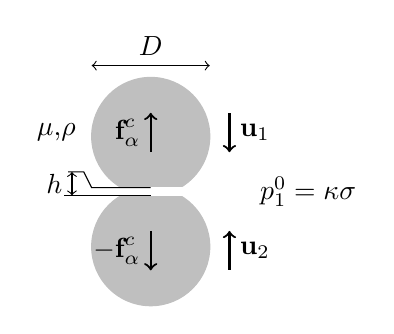
\begin{tikzpicture}
      \draw[lightgray,fill = lightgray] (0,0.7) circle (0.75);
      \draw[lightgray,fill = lightgray] (0,-0.7) circle (0.75);
      \draw[white,fill=white] (-0.75,-0.05) rectangle (0.75,0.05);
      \draw(0,0.05)--++(-0.75,0)--++(-0.1,0.2)--++(-0.2,0);
      \draw(0,-0.05)--++(-1.1,0);
      \draw[<->](-1,-0.05) --++ (0,0.3)node[midway,left]{$h$};
      \draw[<->](-0.75,1.6)--++(1.5,0)node[midway,above]{$D$};
      \node (para) at (-1.2,0.75){$\mu$,$\rho$};
      \node (pressure) at (2,0){$p_1^0 = \kappa \sigma$};
      \draw[->,thick](0,0.5)--++(0,0.5)node[midway,left]{$\textbf{f}_\alpha^\text{c}$};
      \draw[->,thick](0,-0.5)--++(0,-0.5)node[midway,left]{$-\textbf{f}_\alpha^\text{c}$};
      \draw[<-,thick](1,0.5)--++(0,0.5)node[midway,right]{$\textbf{u}_1$};
      \draw[<-,thick](1,-0.5)--++(0,-0.5)node[midway,right]{$\textbf{u}_2$};
    \end{tikzpicture}
    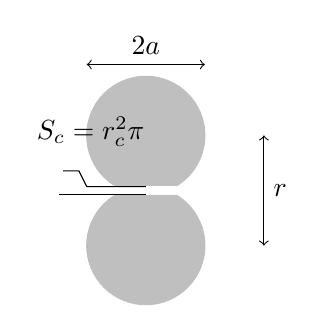
\begin{tikzpicture}
      \draw[lightgray,fill = lightgray] (0,0.7) circle (0.75);
      \draw[lightgray,fill = lightgray] (0,-0.7) circle (0.75);
      \draw[white,fill=white] (-0.75,-0.05) rectangle (0.75,0.05);
      \draw(0,0.05)--++(-0.75,0)--++(-0.1,0.2)--++(-0.2,0);
      \draw(0,-0.05)--++(-1.1,0);
      \draw[<->](-0.75,1.6)--++(1.5,0)node[midway,above]{$2 a$};
      \draw[<->](1.5,0.7)--++(0,-1.4)node[midway,right]{$r$};
      \node (para) at (-0.7,0.75){$S_c = r_c^2 \pi$};
    \end{tikzpicture}
    \caption{Scheme of two colliding droplets at close contact. Notice the null kurvature in the region of the interface close to the film leading to a capilary force $\textbf{f}_\alpha^\text{c} \approx - S_c \kappa \sigma \textbf{r}/|\textbf{r}|$. }
\end{figure}

Let use the following notation $(\bm{\sigma}_1' \cdot \textbf{n}_1)^\Sigma = \textbf{f}_\alpha = \textbf{f}_\alpha^\text{h}+\textbf{f}_\alpha^\text{c}$. 
It is clear, since the mean stress contribution $\div \bm{\sigma}_1$ isn't taken in account inside the drag force term, that the contribution $\textbf{f}_\alpha^\text{h}$ vanish or is negligible compared to $\textbf{f}_\alpha^\text{c}$ when the nearest particle is at a distance $|\textbf{r}| < a$ where $a$ is the.  Radius. 

If there is strong inhomogeneous structure in the flow the pure drag force term might be modified to yields the particle fluid particle stress. 
\begin{align*}
    n_p (\bm{\sigma}_1' \cdot \textbf{n}_1)_p^\Sigma
    &= 
    \int_{\mathrm{R}^3} (\bm{\sigma}_1' \cdot \textbf{n}_1)_\text{nst}^\Sigma
    P_\text{nst}(\textbf{x}\pm\textbf{r}/2,\mp\textbf{r}) d\textbf{r}
    +\div \int_{\mathrm{R}^3} \textbf{r} (\bm{\sigma}_1' \cdot \textbf{n}_1)_\text{nst}^\Sigma
    P_\text{nst}(\textbf{x},\textbf{r}) d\textbf{r}\\
\end{align*}
Which can be again decomposed into : 
\begin{align*}
    n_p (\bm{\sigma}_1' \cdot \textbf{n}_1)_p^\Sigma
    &= 
    \frac{1}{2}\int_{\mathrm{R}^3} \textbf{f}^h_\text{nst}P_\text{nst}(\textbf{x}\pm\textbf{r}/2,\mp\textbf{r}) d\textbf{r}
    + \frac{1}{2}\int_{\mathrm{R}^3} \textbf{f}^c_\text{nst}P_\text{nst}(\textbf{x}\pm\textbf{r}/2,\mp\textbf{r}) d\textbf{r} \\
    &
    +\div \int_{\mathrm{R}^3} \textbf{r} \textbf{f}_\text{nst}^\text{h} P_\text{nst}(\textbf{x},\textbf{r}) d\textbf{r}
    +\div \int_{\mathrm{R}^3} \textbf{r} \textbf{f}_\text{nst}^\text{c} P_\text{nst}(\textbf{x},\textbf{r}) d\textbf{r}\\
\end{align*}
The first term is the pure drag force components. 
The second terms is the pure contact force components which we will see to be null in the next section. 
Then, the third term is the particle-fluid-particle stress. 
And the last is the particle-film-particle stress. 


\subsubsection*{The contact forces}
In the same spirit as the classical surface force, as it is defined in \citet{jackson1997locally,zhang1997momentum,nott2011suspension} we can argue that the ensemble average of the close contact force cancel out. 
More precisely, the contact force on a single particle labeled $i$ due to the close contact with particle $j$ can be modeled by, 
\begin{equation*}
    \textbf{f}_{ij}^\text{c}
    = S_c \kappa \sigma \textbf{r}_{ij}/r_{ij}
    = \pi r_c^2 \kappa \sigma \textbf{r}_{ij}/r_{ij}
    = \pi (a^2 - r_{ij}^2/4) \kappa \sigma  \textbf{r}_{ij}/r_{ij}
\end{equation*} 
The resultants of these forces on the particle $i$ is therefore the sum of the contact with all particles except the $j^\text{th}$ particle, 
\begin{equation*}
    \textbf{f}_{i}^\text{c}
    = \sum_{j \neq i}\textbf{f}_{ij}
    = - \sum_{j \neq i} \pi (a^2 - r_{ij}^2/4) \kappa \sigma \textbf{r}_{ij}/r_{ij}
\end{equation*} 
The ensemble average of this force can be written using the classic point particle average,
\begin{align}    
\pavg{\textbf{f}_i^c}
&=
\int \sum_{i} \delta_i 
\textbf{f}_i^c d\PP 
= \int \sum_{i} \sum_{j \neq i} \delta(\textbf{x} - \textbf{x}_i) 
\textbf{f}_{ij}^c d\PP 
\\
\end{align}
Not that $\textbf{f}_{ij} = - \textbf{f}_{ji}$ however $\delta_i \textbf{f}_{ij} \neq - \delta_j\textbf{f}_{ji}$ thus the sum dosen't cancel drictly. 
Thus, following \citet{nott2011suspension,zhang1997momentum} we introduce the sum $\sum_j \delta(\textbf{x}-\textbf{x}_{ij}) \textbf{f}_{ij}^c =0$ where $\textbf{x}_{ij} = \textbf{x}_{ji} = (\textbf{x}_i+\textbf{x}_j)/2$.
Besides, notice that, 
\begin{equation*}
    \delta(\textbf{x} - \textbf{x}_{ij})
    = 
    \delta(\textbf{x} - \textbf{x}_i + ( \textbf{x}_{ij} - \textbf{x}_i))
    =
    \delta(\textbf{x} - \textbf{x}_i )
    - ( \textbf{x}_{ij} - \textbf{x}_i)\cdot \grad \delta(\textbf{x}-\textbf{x}_\alpha)
    +\frac{1}{2} (\textbf{x}_{ij} - \textbf{x}_i)(\textbf{x}_{ij} - \textbf{x}_i) : \grad\grad \delta(\textbf{x}-\textbf{x}_\alpha)
\end{equation*}
using both relation yields, 
\begin{align}    
    \pavg{\textbf{f}_i^c}
    &= \int \sum_{i} \sum_{j \neq i} [
        \delta(\textbf{x} - \textbf{x}_i)
        -\delta(\textbf{x} - \textbf{x}_{ij})]
    \textbf{f}_{ij}^c d\PP 
    \\
    &= \div \int \sum_{i} \sum_{j \neq i} \delta(\textbf{x}-\textbf{x}_i) (\textbf{x}_{ij} - \textbf{x}_i)
    \textbf{f}_{ij}^c d\PP 
    \\
    &= \frac{1}{2}\div \int \sum_{i} \sum_{j \neq i} \delta(\textbf{x}-\textbf{x}_i) (\textbf{x}_{j} - \textbf{x}_i)
    \textbf{f}_{ij}^c d\PP 
\end{align}
Using the formula for the contact force gives 
\begin{align}    
    \pavg{\textbf{f}_i^c}
    &= \frac{1}{2}\div \int \sum_{i} \sum_{j \neq i} \delta(\textbf{x}-\textbf{x}_i) 
    \textbf{r}\textbf{r}
    \pi (r^2/4 - a^2) /r \kappa \sigma d\PP 
    \\
\end{align}


\subsubsection*{Nearest stats for contacts forces in dilute case}
In the dilute case we consider only one conatc force so that, 
\begin{equation}
    n_p \textbf{f}^c_p = \iint 
    \sum_i 
    \delta(\textbf{x} -\textbf{x}_i)
    \sum_k 
    \textbf{f}_{k \to i}^\text{c} 
    \sum_{j\neq i}
    \delta(\textbf{x} + \textbf{r} -\textbf{x}_j) h_{ij}(t,\CC)
    d\PP d\textbf{r}\\
\end{equation}
Now we make use of a trick to cancel the pair particles forces by notticing that, 
\begin{equation}
    n_p \textbf{f}^c_p = \iint 
    \sum_k 
    \delta(\textbf{x} -\textbf{x}_k)
    \sum_i
    \textbf{f}_{i\to k}^\text{c} 
    \sum_{j\neq k}
    \delta(\textbf{x} + \textbf{r} -\textbf{x}_j) h_{kj}(t,\CC)
    d\PP d\textbf{r}\\
\end{equation}
So, we have, 
\begin{equation}
    n_p \textbf{f}^c_p = \frac{1}{2}\iint 
    \sum_i 
    \sum_k 
    \left[
        \sum_{j\neq i}
        \delta(\textbf{x} -\textbf{x}_i)
        \delta(\textbf{x} + \textbf{r} -\textbf{x}_j) h_{ij}
        \textbf{f}_{k \to i}^\text{c} 
        +
        \sum_{j\neq k}
        \delta(\textbf{x} -\textbf{x}_k)
        \delta(\textbf{x} + \textbf{r} -\textbf{x}_j) h_{kj}
        \textbf{f}_{i \to k}^\text{c} 
    \right]
    d\PP d\textbf{r}\\
\end{equation}
Note that the sums do not have the same restrictions. 
Nevertheless, this can be neglected since, if for example, $j=i$ we obtain $\delta(\textbf{x}-\textbf{x}_i)\delta(\textbf{x}+\textbf{r}-\textbf{x}_i) = 0$ thus the term cancel unless $\textbf{r}=0$ but let neglect that.
Besides, we must define manually that $h_{ii} = 0$ but it doesn't really matter.   
Or we get out these specifics case such as,
\begin{align}
    n_p \textbf{f}^c_p 
    &= \frac{1}{2}\iint 
    \sum_i 
    \sum_k 
    \sum_{j\neq k,i}
    \left[
        \delta(\textbf{x} -\textbf{x}_i)
        \delta(\textbf{x} + \textbf{r} -\textbf{x}_j) h_{ij}
        \textbf{f}_{k \to i}^\text{c} 
        +
        \delta(\textbf{x} -\textbf{x}_k)
        \delta(\textbf{x} + \textbf{r} -\textbf{x}_j) h_{kj}
        \textbf{f}_{i \to k}^\text{c} 
    \right]
    d\PP d\textbf{r}\\
    &+ \frac{1}{2}\iint 
    \sum_i 
    \sum_k 
    \left[
        \delta(\textbf{x} -\textbf{x}_i)
        \delta(\textbf{x} + \textbf{r} -\textbf{x}_k) h_{ik}
        \textbf{f}_{k \to i}^\text{c} 
        +
        \delta(\textbf{x} -\textbf{x}_k)
        \delta(\textbf{x} + \textbf{r} -\textbf{x}_i) h_{ki}
        \textbf{f}_{i \to k}^\text{c} 
    \right]
    d\PP d\textbf{r}\\
\end{align}

Now we must verify that this framework is coherent with the nearest particle statistics framework.
First we recall the definition of the pure drag term of the contact forces according to the neaerst particle statistics. 
\begin{align*}
    \pavg{\textbf{f}_i^\text{c}}
    &= \frac{1}{2}\int \nstavg{\textbf{f}_i^\text{c}} P_\text{nst}(\textbf{x}\pm\textbf{r}/2,\mp \textbf{r}) d\textbf{r}\\
    &=
    \frac{1}{2}\iint \sum_i \sum_{j\neq i}
    \delta(\textbf{x} \pm \textbf{r}/2 -\textbf{x}_i) 
    \delta(\textbf{x} \mp \textbf{r} -\textbf{x}_j) h_{ij}
    \textbf{f}_i^\text{c} 
    d\PP d\textbf{r}\\
    &=
    \frac{1}{2}\iint \sum_i \sum_{j\neq i}
    \delta(\textbf{x} \pm \textbf{r}/2 -\textbf{x}_i)
    \delta(\textbf{x} \mp \textbf{r} -\textbf{x}_j) h_{ij}
    \sum_{k} \textbf{f}_{ik}^\text{c} 
    d\PP d\textbf{r}\\
    &=
    \frac{1}{2}\iint \sum_i \sum_{j\neq i}
    \delta(\textbf{x} \pm \textbf{r}/2 -\textbf{x}_i)
    \delta(\textbf{x} \mp \textbf{r} -\textbf{x}_j) h_{ij}
     (\textbf{f}_{ij}^\text{c} + \sum_{k\neq i,j} \textbf{f}_{ik}^c)
    d\PP d\textbf{r}
\end{align*}
We must verify that both component of this integral cancel out. 
Changing teh integration sign we get,
\begin{equation*}
    \int \nstavg{\textbf{f}_i^\text{c}} P_\text{nst}(\textbf{x}, \textbf{r}) d\textbf{r}
    = \int \nstavg{\textbf{f}_i^\text{c}} P_\text{nst}(\textbf{x}, - \textbf{r}) d\textbf{r}
\end{equation*}
The drag force can alse, be written, 
\begin{equation*}
    \int [\textbf{f}^c_\text{eb}(\textbf{x}+\textbf{r}/2,\textbf{x} - \textbf{r}/2)+ \textbf{f}_\text{eb}^c(\textbf{x} -\textbf{r}/2,\textbf{x}+ \textbf{r}/2)]P_2(\textbf{x}\pm\textbf{r}/2,\textbf{x}\mp \textbf{r}/2) d\textbf{r}
    = \\
\end{equation*}
And since the contact force has only an antisymmetric contribution in average it is always true that in an averaged sense we have $\nstavg{\textbf{f}_i^\text{c}} P_\text{nst}(\textbf{x}, \textbf{r})  = - \nstavg{\textbf{f}_i^\text{c}} P_\text{nst}(\textbf{x}, - \textbf{r}) $, 
Additionally, 
\begin{align*}
    \pavg{\textbf{f}_\text{eb}^\text{c}}
    &=
    \frac{1}{2}\iint \sum_i \sum_{j\neq i}
    \delta(\textbf{x} + \textbf{r}/2 -\textbf{x}_i)
    \delta(\textbf{x} - \textbf{r}/2 -\textbf{x}_j) h_{ij}
    \sum_{k \neq i} \textbf{f}_{ik}^\text{c} 
    d\PP d\textbf{r}\\
    &=
    \frac{1}{2}\iint \sum_i \sum_{j\neq i}
    \delta(\textbf{x} + \textbf{r}/2 -\textbf{x}_i)
    \delta(\textbf{x} - \textbf{r}/2 -\textbf{x}_j) 
    h_{ij}
    \sum_{k \neq i} \textbf{f}_{ik}^\text{c} 
    d\PP d\textbf{r}\\
\end{align*}

\begin{align}    
\pavg{\textbf{f}_i^c}
&= \int_{|\textbf{r}|<a}
\int \sum_{i \neq j} \delta_i \sum_{j\neq i} \delta_j h_{ij}
\textbf{f}_i^c d\PP d\textbf{r}
= \int_{|\textbf{r}|<a}
\int \sum_{i \neq j} \delta_i \sum_{j\neq i} \delta_j h_{ij}
\sum_{k\neq i} \pi (r_{ik}^2/4 - a^2) \kappa \sigma \textbf{r}_{ik}/r_{ik} d\PP d\textbf{r}\\
&= \int_{|\textbf{r}|<a}
\int \sum_{i \neq j} \delta_i \sum_{j\neq i} \delta_j h_{ij}
\sum_{k\neq i} \pi (r_{ik}^2/4 - a^2) \kappa \sigma \textbf{r}_{ik}/r_{ik} d\PP d\textbf{r}
\\
\end{align}

Anyhow if we lake the assumption that this term indeed cancel we arrive at the expression: 
\begin{equation*}
    \int_{\mathrm{R}^3} \textbf{r} \textbf{f}_\text{nst}^\text{c} P_\text{nst}(\textbf{x},\textbf{r}) d\textbf{r}
    = 
\end{equation*}

\section{The dumping model}

Let decompose the drag force such that $\textbf{f}_\alpha = \textbf{f}_\alpha^h + \textbf{f}_\alpha^c$ with $^h$ being the hydrodynamical forces and $\textbf{f}^c_\alpha$ being the contatc forces. 
Let assume that the particle $\alpha$ interact with the particle $\beta$, where both particles has a radius $a$.
Let note $\textbf{r} = (\textbf{x}_\alpha - \textbf{x}_\beta) = \textbf{n} a$. 
Now let consider that the contact force can be modeled as a spring/dumping model with $k$ being the \textit{Raideur} and $c$ the dumping coefficient.
Then, the contact force between both particles can be written as, 
\begin{equation}
    \textbf{f}_\beta^c
    = \textbf{f}_{\alpha\beta}
    = (|\textbf{r}| - a) \textbf{n} k 
    + (\textbf{u}_\alpha - \textbf{u}_\beta) c
    \;\;\;\;\text{for} \;\;\; (|\textbf{r}| - a) < 0
\end{equation}
For smooth particle the second term can be reduced to the components along the normal vector \textbf{n}.  
Due to Newton's  law and since each interaction force cancel each other we have $\avg{\textbf{f}_\beta^c} \approx 0$. 
However, it is useful to notice that we have in the case of inhomogeneous scenario $\avg{\textbf{f}_\beta^c} \approx - \div \Sigma^c$.

Now let's focus on the source term of the granular temperature $\avg{\textbf{f}_\alpha\cdot \textbf{u}_\alpha'} = \avg{\textbf{f}_\alpha^h \cdot \textbf{u}_\alpha'} + \avg{\textbf{f}_\alpha^c\cdot \textbf{u}_\alpha'}$. 
The first source term $\avg{\textbf{f}_\alpha^h \cdot \textbf{u}_\alpha'} \sim k_p$ since $\textbf{f}_\alpha \sim \textbf{u}_\alpha$.

The part due to collision can be re written using the nearest averaged statistics formalism, 
\begin{align*}
    \avg{\textbf{f}_\alpha^c\cdot \textbf{u}_\alpha'}
    &= \int_{\textsc{R}^3}
    \int \sum_{\alpha \neq \beta} \delta_\alpha \delta_\beta h_{\alpha\beta}
    \textbf{u}'_\alpha \textbf{f}_\alpha^c d\PP d\textbf{r}\\
    &= \int_{\textsc{R}^3}
    \int \sum_{\alpha \neq \beta} \delta_\alpha \delta_\beta h_{\alpha\beta}
    \textbf{u}'_\alpha \cdot \textbf{n}
        (|\textbf{r}| - a) 
     d\PP d\textbf{r}
    + \int_{\textsc{R}^3}
    \int \sum_{\alpha \neq \beta} \delta_\alpha \delta_\beta h_{\alpha\beta}
    \textbf{u}'_\alpha 
         (\textbf{u}_\alpha - \textbf{u}_\beta) c
     d\PP d\textbf{r}\\
    &=k \int_{|\textbf{r}|<a}
    \nstavg{\textbf{u}'_\alpha \cdot \textbf{n}
        (|\textbf{r}| - a)   }
        P_{nst}(\textbf{x},\textbf{r})
     d\textbf{r}
    +c \int_{|\textbf{r}|<a}
        \nstavg{\textbf{u}'_\alpha 
         \cdot (\textbf{u}_\alpha - \textbf{u}_\beta)} P_\text{nst}(\textbf{x},\textbf{r})
     d\textbf{r}\\
\end{align*}
Elastic collisions are not dissipative therefore the first term cancel by definition. 
Thus, we are left with, 
\begin{align*}
    \avg{\textbf{f}_\alpha^c\cdot \textbf{u}_\alpha'}
    = c \int_{|\textbf{r}|<a}
        \nstavg{\textbf{u}'_\alpha 
         \cdot (\textbf{u}_\alpha - \textbf{u}_\beta)} P_\text{nst}(\textbf{x},\textbf{r})
     d\textbf{r} 
\end{align*}
\subsection{The dispersed phase equations}

Regarding the dispersed phase, we found the mass, momentum and total energy balance equations, 
\begin{align*}
    \pddt \left(n_p m_p\right)
    + \div \left(n_pm_p\textbf{u}_p
    \right)
    = 
    0\\
    \pddt \left(n_p m_p \textbf{u}_p\right)
    + \div \left(n_p
    m_p \textbf{u}_p \textbf{u}_p 
    - \bm{\sigma}_p^\text{eq}
    \right)
    = 
    n_p v_p  (  
    \rho_2 \textbf{g}
    - \grad p_1)
    + n_p (\bm{\sigma}_1'\cdot \textbf{n}_2)_p^\Sigma,\\
    \pddt(m_p n_pE_p^\text{tot})
    + \div(m_pn_p E_p^\text{tot} \textbf{u}_p 
    + \textbf{q}_p^\text{eq} - \textbf{u}_p \cdot \bm{\sigma}_p^\text{eq})
    =  n_p v_p [\rho_2 \textbf{u}_p\cdot  \textbf{g} 
    - \div (\textbf{u}_1 p_1)]\\
    +  n_p ( \textbf{u}'_1 \cdot \bm{\sigma}_1^0 \cdot \textbf{n}_2)_p^\Sigma
    -  n_p (\textbf{q}_1^0 \cdot \textbf{n}_2)_p^\Sigma
    +  n_p (\textbf{u}_1 \cdot \bm{\sigma}_1'\cdot \textbf{n}_2)_p^\Sigma
\end{align*}
where we have defined, 
\begin{align*}
    &\bm{\sigma}_p^\text{eq}
    = -  m_p\pnavg{\textbf{u}_\alpha'\textbf{u}_\alpha'}
    &\textbf{q}_p^\text{eq}
    =\textbf{q}_p^\text{e} 
    +\textbf{q}_p^\text{k}  
    +\textbf{q}_p^\text{w}  
    \\
    &\textbf{q}_1^\text{e}
    = m_p \pnavg{\textbf{u}_\alpha' e_\alpha'} 
    &\textbf{q}_p^\text{k}
    = m_p \pnavg{\textbf{u}_\alpha' k_\alpha} 
    \\
    &\textbf{q}_p^\text{w}
    = 
    + \pnavg{\textbf{u}_\alpha'(\rho_2 (w^0_2)^2/2 )'_\Omega}
    + \gamma \pnavg{\textbf{u}_\alpha' s_\alpha'}
\end{align*}

Now, subtracting each of these equations to the total NRJ equations yields, 


\tb{Think about doing a surface equation ? ? }
At the Lagrangian scale, 
\begin{equation*}
    \pavg{\ddt (m_\alpha E_\alpha + s_\alpha \gamma)}
    = 
     n_p (\rho_2 \textbf{u}_2^0  \cdot \textbf{g})^\Omega_p
    +n_p (\textbf{u}_1^0 \cdot \bm{\sigma}_1^0 \cdot  \textbf{n}_2)^\Sigma_p
    - n_p (\textbf{q}_1^0 \cdot \textbf{n}_2)^\Sigma_p
\end{equation*}
\begin{align}
    \pavg{\frac{1}{2}\ddt (m_\alpha u_\alpha^2)}
    &= 
    n_p (\rho_2 \textbf{u}_2^0 \cdot
    \textbf{g})_p^\Omega
    + 
    (\textbf{u}_\alpha\cdot
    \textbf{f}_\alpha)_p\\
    \pavg{\frac{1}{2}\ddt \left[\int_{\Omega_\alpha} \rho_2 (w_2^0)^2 d\Omega +s_\alpha \gamma\right] }
    &= (\textbf{w}_1^0 \cdot (\bm{\sigma}_1^0 \cdot \textbf{n}_2) )_p^\Sigma  
     - (\bm{\sigma}_2^0 : \grad\textbf{u}_2^0)_p^\Omega  
    \\
    \pavg{\ddt (m_\alpha e_\alpha )}
    &= 
     + n_p (\bm{\sigma}_2^0 : \grad\textbf{u}_2^0)^\Omega_p
    -  n_p (\textbf{q}_1^0 \cdot \textbf{n}_2 )_p^\Sigma
\end{align}
We first notice that, 
\begin{equation*}
    n_p\frac{1}{2}(m_\alpha u_\alpha^2)_p
    = n_p\frac{1}{2}m_p u_p^2
    +  k_p
\end{equation*}
Deriving the momentum kinetic NRJ equation for the particle phase and the above else we can have the following system of equations. 
\begin{align*}
    &\pddt \left(n_p m_p u_p^2/ 2\right)
    + \div \left(n_p
    m_p u_p^2/ 2 \textbf{u}_p 
    - \textbf{u}_p \cdot \bm{\sigma}_p^\text{eq}
    \right)
    = 
    - \bm{\sigma}_p^\text{eq}  :\grad \textbf{u}_p
    +  n_p v_p \textbf{u}_p \cdot (
    \rho_2 \textbf{g}
    - \grad p_1 )
    + n_p \textbf{u}_p \cdot (\bm{\sigma}'_1 \cdot \textbf{n}_2)^\Sigma_p,\\
    &\pddt \left(n_p (\rho_2 w^2 )_p^\Omega+\gamma s_p n_p\right)
    + \div 
    (n_p (\rho_2 w^2 )_p^\Omega+\gamma s_p n_p)
    \textbf{u}_p 
    +  \textbf{q}_p^\text{w}
    )
    = \\
    &- n_p (\bm{\sigma}_2^0 : \grad\textbf{u}_2^0)^\Omega_p
    + n_p (\textbf{u}_1 \cdot \bm{\sigma}_1' \cdot  \textbf{n}_2)^\Sigma_p
    + n_p (\textbf{u}_1' \cdot \bm{\sigma}_1^0 \cdot  \textbf{n}_2)^\Sigma_p
    -n_p v_p \grad (\textbf{u}_1p_1)
    - n_p (\textbf{u}_\alpha \cdot \bm{\sigma}_1^0 \cdot  \textbf{n}_2)^\Sigma_p
    \\
    &\pddt \left(n_p m_p e_p\right)
    + \div \left(n_p
    m_p e_p \textbf{u}_p 
    +  \textbf{q}_p^\text{e}
    \right)
    = 
    + n_p (\bm{\sigma}_2^0 : \grad\textbf{u}_2^0)^\Omega_p
    - n_p (\textbf{q}_1^0\cdot \textbf{n}_2)^\Sigma_p\\
\end{align*}

Now if we subtract these from the total NRJ equation one can show, 
\begin{multline*}
    \pddt(m_p n_pk_p)
    + \div(m_pn_p k_p \textbf{u}_p 
    + \textbf{q}_p^\text{k})
    = 
     \bm{\sigma}_p^\text{eq}  :\grad \textbf{u}_p
     + n_p v_p \textbf{u}_p \grad p_1
     + n_p (\textbf{u}_\alpha \cdot \bm{\sigma}_1^0 \cdot  \textbf{n}_2)^\Sigma_p
     - n_p \textbf{u}_p \cdot (\bm{\sigma}_1' \cdot  \textbf{n}_2)^\Sigma_p
    \\
\end{multline*}
Notice that, 















In order to be consistent with the fluid phase equations these terms must be written with $\textbf{f}_\text{pm} = n_p\textbf{u}_1 \cdot ((\bm{\sigma}_1^0 \cdot  \textbf{n}_2)^\Sigma_{nst}(\textbf{x} \pm \textbf{r}/2,\mp\textbf{r}) )_p$, and espetially  $\textbf{f}_\text{pm} = n_p ((\textbf{u}_1' \cdot\bm{\sigma}_1^0 \cdot  \textbf{n}_2)^\Sigma_{nst}(\textbf{x} \pm \textbf{r}/2,\pm\textbf{r}))_p$. Thus we need to reformulate. 
We use, 
\begin{align*}
    n_p (\bm{\sigma}_1^0 \cdot  \textbf{n}_2)^\Sigma_p
    = 
    n_p ( \bm{\sigma}_1' \cdot  \textbf{n}_2)^\Sigma_p
    - n_p (p_1   \textbf{n}_2)^\Sigma_p\\
    n_p (\textbf{u}_1^0 \cdot \bm{\sigma}_1^0 \cdot  \textbf{n}_2)^\Sigma_p
    = 
    n_p (\textbf{u}_1 \cdot \bm{\sigma}_1' \cdot  \textbf{n}_2)^\Sigma_p
    + n_p (\textbf{u}_1' \cdot \bm{\sigma}_1^0 \cdot  \textbf{n}_2)^\Sigma_p
    - n_p (\textbf{u}_1 p_1 \cdot  \textbf{n}_2)^\Sigma_p
\end{align*}
Notice that $\textbf{u}_1$ and $p_1$ varies slowly inside the volume of the particle.
Consequently we must use the relation, $\textbf{u}_1(\textbf{r}) = \textbf{u}_1(\textbf{x}_\alpha) + \textbf{r} \cdot\grad \textbf{u}_1(\textbf{x}_\alpha) \ldots$
and $p_1(\textbf{r}) = p_1(\textbf{x}_\alpha) + \textbf{r} \cdot\grad p_1(\textbf{x}_\alpha) \ldots$
to finnaly obtain, 
\begin{align*}
    n_p (\bm{\sigma}_1^0 \cdot  \textbf{n}_2)^\Sigma_p
    &= 
    n_p ( \bm{\sigma}_1' \cdot  \textbf{n}_2)^\Sigma_p
    - n_p v_p \grad p_1\\
    n_p (\textbf{u}_1^0 \cdot \bm{\sigma}_1^0 \cdot  \textbf{n}_2)^\Sigma_p
    &= 
    n_p (\textbf{u}_1 \cdot \bm{\sigma}_1' \cdot  \textbf{n}_2)^\Sigma_p
    + n_p (\textbf{u}_1' \cdot \bm{\sigma}_1^0 \cdot  \textbf{n}_2)^\Sigma_p
    - n_p v_p \div (\textbf{u}_1 p_1) \\
    &= 
    n_p \textbf{u}_1 \cdot( \bm{\sigma}_1' \cdot  \textbf{n}_2)^\Sigma_p
    + n_p (\textbf{r} \bm{\sigma}_1' \cdot  \textbf{n}_2)^\Sigma_p : \grad \textbf{u}_1
    + n_p (\textbf{u}_1' \cdot \bm{\sigma}_1^0 \cdot  \textbf{n}_2)^\Sigma_p
    - n_p v_p \div (\textbf{u}_1 p_1) \\
    &= 
    n_p \textbf{u}_1 \cdot \textbf{f}_{pm}
    + n_p (\mathcal{F}_p - \mathcal{F}_\text{pfp}): \grad \textbf{u}_1
    + n_p \textbf{c}_\text{pm}
    + \div [n_p(\mathcal{C}_\text{pfp} + \textbf{u}_1 \cdot \mathcal{F}_\text{pfp})]
    - n_p v_p \div (\textbf{u}_1 p_1) 
\end{align*}

\begin{align*}
    n_p (\textbf{w}_1^0 \cdot \bm{\sigma}_1^0 \cdot  \textbf{n}_2)^\Sigma_p
    &= 
    n_p (\textbf{u}_1^0 \cdot \bm{\sigma}_1^0 \cdot  \textbf{n}_2)^\Sigma_p
    - n_p (\textbf{u}_\alpha \cdot \bm{\sigma}_1^0 \cdot  \textbf{n}_2)^\Sigma_p\\
    n_p (\textbf{u}_\alpha \cdot \bm{\sigma}_1^0 \cdot  \textbf{n}_2)^\Sigma_p
    &=
    n_p (\textbf{u}_\alpha \cdot \bm{\sigma}_1' \cdot  \textbf{n}_2)^\Sigma_p
    - n_p (\textbf{u}_\alpha \cdot p_1 \cdot  \textbf{n}_2)^\Sigma_p
    % n_p (\textbf{u}_1 \cdot \bm{\sigma}_1' \cdot  \textbf{n}_2)^\Sigma_p
    % + n_p (\textbf{u}_1' \cdot \bm{\sigma}_1^0 \cdot  \textbf{n}_2)^\Sigma_p
    % - n_p v_p \div (\textbf{u}_1 p_1) \\
\end{align*}

In fact if we start back from the exact relation defined in the continuous pahse we can say that ,
\begin{align*}
    \avg{\delta_I (\bm{\sigma}_1^0 ) \textbf{n}_2} - p_1 \grad \phi_1
    = 
    % \avg{\delta_I (\bm{\sigma}_1^0 + p_1)\cdot \textbf{n}_2}
    % = 
    \avg{\delta_I \bm{\sigma}_1'\cdot \textbf{n}_2}
    \\
    \avg{\delta_I (\textbf{u}_1^0 \cdot\bm{\sigma}_1^0 )} - \textbf{u}_1p_1\cdot \grad \phi_1
    % = \avg{\delta_I (\textbf{u}_1 \cdot \bm{\sigma}_1' + \textbf{u}_1' \cdot \bm{\sigma}_1^0 )\cdot \textbf{n}_2}
    = \textbf{u}_1 \cdot \avg{\delta_I \bm{\sigma}_1'\cdot \textbf{n}_2}
    + \avg{\delta_I (\textbf{u}_1' \cdot \bm{\sigma}_1^0 )\cdot \textbf{n}_2}
\end{align*}

incoherence in teh exchange terms, 
\begin{align*}
    n_p (\textbf{u}_\alpha' \cdot \bm{\sigma}_1^0\cdot \textbf{n}_2)^\Sigma_p
    &= \int
    \sum_\alpha \delta_\alpha(\textbf{x} - \textbf{x}_\alpha)
    \textbf{u}_\alpha'(\CC,t)\cdot
    \left[\int_{\Sigma_\alpha} 
     (\bm{\sigma}_1^0 +p_1 \textbf{I})\cdot \textbf{n}_2
     d\textbf{r}
    - \int_{\Sigma_\alpha} 
     p_1  \textbf{n}_2
     d\textbf{r}\right]
     d\PP \\
    &= \int
    \sum_\alpha \delta_\alpha(\textbf{x} - \textbf{x}_\alpha)
    \textbf{u}_\alpha'(\CC,t)\cdot
    \left[\int_{\Sigma_\alpha} 
     \bm{\sigma}_1' +\cdot \textbf{n}_2
     d\textbf{r}
    - v_\alpha \grad p_1(\textbf{x}_\alpha)
    \right]
     d\PP \\
    &= n_p (\textbf{u}_\alpha' \cdot (\bm{\sigma}'_1\cdot \textbf{n}_2)^\Sigma )_p
    -  n_p (\textbf{u}_\alpha' v_p \cdot \grad p_1 )_p
     \\
    &= n_p (\textbf{u}_\alpha' \cdot (\bm{\sigma}'_1\cdot \textbf{n}_2)^\Sigma )_p
     \\
\end{align*}
Since $\textbf{u}_p$ is an Eulerian fields it must be evaluated at $\textbf{r}$ Therefore it must get out the 

Also, 
\begin{align*}
    n_p (\textbf{u}_1' \cdot \bm{\sigma}_1'\cdot \textbf{n}_2)^\Sigma_p
    &= \int
    \sum_\alpha \delta_\alpha(\textbf{x} - \textbf{x}_\alpha)
    \left[\int_{\Sigma_\alpha} 
    \textbf{u}_1'\cdot
    \bm{\sigma}_1^0\cdot \textbf{n}_2
    d\textbf{r}
    + \int_{\Sigma_\alpha} 
    \textbf{u}_1'\cdot
     p_1  \textbf{n}_2
     d\textbf{r}\right]
     d\PP \\
    &= n_p (\textbf{u}_1' \cdot \bm{\sigma}_1^0 \cdot \textbf{n}_2)^\Sigma_p
    -  n_p (\textbf{u}_1'[p_1  +  \textbf{r}\cdot \grad p_1 ]\cdot \textbf{n}_2 )_p^\Sigma
     \\
    &= n_p (\textbf{u}_1' \cdot \bm{\sigma}_1^0 \cdot \textbf{n}_2)^\Sigma_p
    -  n_p p_1  (\div \textbf{u}_1')_p^\Omega
    -  n_p (\textbf{u}_1'[p_1  +  \textbf{r}\cdot \grad p_1 ]\cdot \textbf{n}_2 )_p^\Sigma\\
    &= n_p (\textbf{u}_1' \cdot \bm{\sigma}_1^0 \cdot \textbf{n}_2)^\Sigma_p
    -  n_p\grad p_1\cdot ( \textbf{u}'_1)_p^\Omega
     \\
\end{align*}

Also, 
\begin{align*}
    n_p (\textbf{w}_2^0 \cdot \bm{\sigma}_1^0\cdot \textbf{n}_2)^\Sigma_p
    &= \int
    \sum_\alpha \delta_\alpha(\textbf{x} - \textbf{x}_\alpha)
    \cdot
    \left[\int_{\Sigma_\alpha} 
     \textbf{w}_2^0 (\bm{\sigma}_1^0 +p_1 \textbf{I})\cdot \textbf{n}_2
     d\textbf{r}
    - \int_{\Sigma_\alpha} 
     \textbf{w}_2^0 p_1  \textbf{n}_2
     d\textbf{r}\right]
     d\PP \\
    &= \int
    \sum_\alpha \delta_\alpha(\textbf{x} - \textbf{x}_\alpha)
    \left[\int_{\Sigma_\alpha} 
     \textbf{w}_2^0 \cdot \bm{\sigma}_1'\cdot \textbf{n}_2
     d\textbf{r}
    - \int_{\Sigma_\alpha} 
     \textbf{w}_2^0 (p_1 + \textbf{r}\grad p_1)   \textbf{n}_2
     d\textbf{r}\right]
     d\PP \\
     &= n_p (\textbf{w}_2^0 \cdot \bm{\sigma}_1' \cdot \textbf{n}_2)^\Sigma_p
    - n_p (p_1 \textbf{w}_2^0 \cdot \textbf{n}_2)^\Sigma_p\\
     &= n_p (\textbf{w}_2^0 \cdot \bm{\sigma}_1' \cdot \textbf{n}_2)^\Sigma_p
    - n_p (p_1 (\textbf{w}_2^0 \cdot \textbf{n}_2)^\Sigma)_p
    - n_p (\grad p_1\cdot ( \textbf{r} \textbf{w}_2^0 \cdot \textbf{n}_2)^\Sigma)_p\\
     &= n_p (\textbf{w}_2^0 \cdot \bm{\sigma}_1' \cdot \textbf{n}_2)^\Sigma_p
    - n_p (\grad p_1\cdot ( \div(\textbf{r} \textbf{w}_2^0))^\Omega)_p\\
     &= n_p (\textbf{w}_2^0 \cdot \bm{\sigma}_1' \cdot \textbf{n}_2)^\Sigma_p
    - n_p (\grad p_1\cdot ( \div\textbf{r} \textbf{w}_2^0)^\Omega)_p
    - n_p (\grad p_1\cdot ( \textbf{r} \div\textbf{w}_2^0)^\Omega)_p\\
     &= n_p (\textbf{w}_2^0 \cdot \bm{\sigma}_1' \cdot \textbf{n}_2)^\Sigma_p
\end{align*}







The averaged particle energy $n_p E_p$ can be split into five components,
\begin{equation*}
    n_p m_p E_p(t) 
    = m_p n_p e_p 
    + \pnavg{\int_{\Omega_\alpha(t)} \rho_2  (w_2^0)^2/2 d\Omega}
    + m_p n_p k_p
    + m_p n_p (u_p)^2/2
    + n_p s_p \gamma
    % + \textbf{u}_\alpha \cdot \int_{\Omega_\alpha(t)} \rho_2  \textbf{w}_2^0 d\Omega
\end{equation*}
where $k_p = \pavg{(u_\alpha')^2/2}$.
one equation for each is riquiered 
Using the mass balance and the momentum balance dotted with $\textbf{u}_p$ we obtain the particle kinetic energy balance, 
\begin{align*}
    \pddt \left(n_p m_p u_p^2/ 2\right)
    + \div \left(n_p
    m_p u_p^2/ 2 \textbf{u}_p 
    - \textbf{u}_p \cdot \bm{\sigma}_p^\text{eq}
    \right)
    = 
    - \bm{\sigma}_p^\text{eq}  :\grad \textbf{u}_p
    +  n_p v_p \textbf{u}_p \cdot (
    \rho_2 \textbf{g}
    - \grad p_1 )
    + n_p \textbf{u}_p \cdot \textbf{f}_{pm},\\
    \pddt \left(n_p (\rho_2 w^2 )_p^\Omega+\gamma s_p n_p\right)
    + \div 
    (n_p (\rho_2 w^2 )_p^\Omega+\gamma s_p n_p)
    \textbf{u}_p 
    +  \textbf{q}_p^\text{w}
    )
    = 
    - n_p \textbf{d}_p
    +  n_p (\textbf{u}_1 -\textbf{u}_p) \cdot  (\textbf{f}_{pm} - v_p \grad p_1)
    + n_p\textbf{c}_p\\
    \pddt \left(n_p m_p e_p\right)
    + \div \left(n_p
    m_p e_p \textbf{u}_p 
    +  \textbf{q}_p^\text{e}
    \right)
    = 
    + n_p \textbf{d}_p
    + n_p \textbf{e}_{pm},\\
\end{align*}
\tb{we remark that the collision tensor appear exactly at the same place as the pfp}
Subtracting all 3 equation to the total energy finally gives, 
\begin{align*}
    \pddt(m_p n_pk_p)
    + \div(m_pn_p k_p \textbf{u}_p 
    + \textbf{q}_p^\text{k})
    = 
    \bm{\sigma}_p^\text{eq} : \grad \textbf{u}_p
    % - n_p \textbf{d}_p
    - n_p v_p p_1 \div \textbf{u}_1
    + n_p (( \textbf{u}_\alpha' \cdot \bm{\sigma}_1^0 \cdot \textbf{n}_2)^\Sigma_\text{nst}(\textbf{x}\pm\textbf{r}/2,\mp\textbf{r}) )_p^r \\
\end{align*}
The transfer term of the internal droplets' fluctuation reads, 
\begin{align*}
    \int_{\Sigma_\alpha} \textbf{w}_1^0 \cdot (\bm{\sigma}_1^0 \cdot \textbf{n}_2) d\Sigma  
    = 
    (\textbf{u}_1 -\textbf{u}_\alpha) \cdot \int_{\Sigma_\alpha}  (\bm{\sigma}_1^0 \cdot \textbf{n}_2) d\Sigma  
    + \int_{\Sigma_\alpha} \textbf{u}_1' \cdot (\bm{\sigma}_1^0 \cdot \textbf{n}_2) d\Sigma  
    = (\textbf{u}_1 -\textbf{u}_\alpha) \cdot  (\textbf{f}_\alpha - \grad p_1)
    + \textbf{c}_\alpha
\end{align*}
\begin{align*}
    n_p (\textbf{w}_1^0 \cdot \bm{\sigma}_1^0 \cdot \textbf{n}_2)^\Sigma_p
    &= 
    n_p ((\textbf{w}_1^0 \cdot \bm{\sigma}_1^0 \cdot \textbf{n}_2)^\Sigma_\text{nst}(\textbf{x}\pm\textbf{r}/2,\mp\textbf{r}) )_p^r 
    + \div (n_p ( \textbf{r}(\textbf{w}_1^0 \cdot \bm{\sigma}_1^0 \cdot \textbf{n}_2)^\Sigma_\text{nst}(\textbf{x},\textbf{r}) )_p^r )\\
    &= 
    n_p (((\textbf{u}_1-\textbf{u}_\alpha) \cdot \bm{\sigma}_1^0 \cdot \textbf{n}_2)^\Sigma_\text{nst}(\textbf{x}\pm\textbf{r}/2,\mp\textbf{r}) )_p^r 
    +n_p ((\textbf{u}_1' \cdot \bm{\sigma}_1^0 \cdot \textbf{n}_2)^\Sigma_\text{nst}(\textbf{x}\pm\textbf{r}/2,\mp\textbf{r}) )_p^r \\
    &+ \div [n_p ( \textbf{r}((\textbf{u}_1 - \textbf{u}_\alpha) \cdot \bm{\sigma}_1^0 \cdot \textbf{n}_2)^\Sigma_\text{nst}(\textbf{x},\textbf{r}) )_p^r 
    + n_p ( \textbf{r}(\textbf{u}_1' \cdot \bm{\sigma}_1^0 \cdot \textbf{n}_2)^\Sigma_\text{nst}(\textbf{x},\textbf{r}) )_p^r ]\\
    &= 
    n_p (((\textbf{u}_1-\textbf{u}_\alpha) \cdot \bm{\sigma}_1^0 \cdot \textbf{n}_2)^\Sigma_\text{nst}(\textbf{x}\pm\textbf{r}/2,\mp\textbf{r}) )_p^r 
    +n_p \textbf{c}_{pm} \\
    &+ \div [n_p ( \textbf{r}((\textbf{u}_1 - \textbf{u}_\alpha) \cdot \bm{\sigma}_1^0 \cdot \textbf{n}_2)^\Sigma_\text{nst}(\textbf{x},\textbf{r}) )_p^r 
    + n_p \mathcal{C}_\text{pfp}]\\
\end{align*}
The remaining terms can be expressed as, 
\begin{align*}
    n_p (((\textbf{u}_1-\textbf{u}_\alpha) \cdot \bm{\sigma}_1^0 \cdot \textbf{n}_2)^\Sigma_\text{nst}(\textbf{x}\pm\textbf{r}/2,\mp\textbf{r}) )_p^r 
    &= 
    n_p (\textbf{u}_1 - \textbf{u}_p) \cdot (( \bm{\sigma}_1^0 \cdot \textbf{n}_2)^\Sigma_\text{nst}(\textbf{x}\pm\textbf{r}/2,\mp\textbf{r}) )_p^r \\
    &- n_p (( \textbf{u}_\alpha' \cdot \bm{\sigma}_1^0 \cdot \textbf{n}_2)^\Sigma_\text{nst}(\textbf{x}\pm\textbf{r}/2,\mp\textbf{r}) )_p^r \\
    &= 
    n_p (\textbf{u}_1 - \textbf{u}_p) \cdot(\textbf{f}_p - \grad p_1) \\
    &- n_p (( \textbf{u}_\alpha' \cdot \bm{\sigma}_1^0 \cdot \textbf{n}_2)^\Sigma_\text{nst}(\textbf{x}\pm\textbf{r}/2,\mp\textbf{r}) )_p^r \\
\end{align*}
The higher moments terms can be expressed as, 
\begin{align*}
    n_p (\textbf{r}((\textbf{u}_1-\textbf{u}_\alpha) \cdot \bm{\sigma}_1^0 \cdot \textbf{n}_2)^\Sigma_\text{nst})_p^r 
    &= 
    n_p (\textbf{u}_1 - \textbf{u}_p) \cdot (\textbf{r} ( \bm{\sigma}_1^0 \cdot \textbf{n}_2)^\Sigma_\text{nst} )_p^r 
    - n_p ( \textbf{r} ( \textbf{u}_\alpha' \cdot \bm{\sigma}_1^0 \cdot \textbf{n}_2)^\Sigma_\text{nst} )_p^r \\
    &= 
    n_p (\textbf{u}_1 - \textbf{u}_p)\cdot \mathcal{F}_\text{pfp} 
    - n_p (\textbf{r} ( \textbf{u}_\alpha' \cdot \bm{\sigma}_1^0 \cdot \textbf{n}_2)^\Sigma_\text{nst} )_p^r \\
\end{align*}
Alternatively, without the nearest particle formalism we obtain, 
\begin{align*}
    n_p (\textbf{w}_1^0 \cdot \bm{\sigma}_1^0 \cdot \textbf{n}_2)^\Sigma_p
    &= 
    n_p ((\textbf{w}_1^0 \cdot \bm{\sigma}_1^0 \cdot \textbf{n}_2)^\Sigma)_p 
\end{align*}

Averaging the microscopic 
\begin{align}
    \frac{1}{2}\ddt (m_\alpha u_\alpha^2)
    &= 
    \textbf{u}_\alpha\cdot
    \textbf{g}m_\alpha
    + 
    \textbf{u}_\alpha\cdot
    \textbf{f}_\alpha\\
    \frac{1}{2}\ddt \int_{\Omega_\alpha} \rho_2 (w_2^0)^2 d\Omega 
    + \ddt (s_\alpha \gamma) 
    &= 
    \int_{\Sigma_\alpha} \textbf{w}_1^0 \cdot (\bm{\sigma}_1^0 \cdot \textbf{n}_2) d\Sigma  
     - \int_{\Omega_\alpha} \bm{\sigma}_2^0 : \grad\textbf{u}_2^0 d\Omega  
    \\
    \ddt (m_\alpha e_\alpha )
    &= 
     \int_{\Omega_\alpha} \bm{\sigma}_2^0 : \grad\textbf{u}_2^0 d\Omega  
    -  s_\alpha \textbf{q}_\alpha  
\end{align}
Additionally, we can add an equation for the first moment of momentum, 
\begin{multline}
    \pddt \left(n_p \mathcal{P}_p\right)
    + \div \left(
        n_p \textbf{u}_p \mathcal{P}_p
    + \Sigma_p^\text{eq}
    \right)
    =
    n_p v_p \bm{\sigma}_1 
    + n_p \mathcal{F}_p\\
    +\pnavg{\int_{\Omega_\alpha} \left(
        \rho_2 \textbf{w}_2^0  \textbf{w}_2^0 
        - \bm{\sigma}_2^0
        \right) d\Omega}
        - \gamma  \pnavg{\int_{\Sigma_\alpha} \textbf{I}_{||} d\Sigma},
\end{multline}



\subsubsection{Modeling of collisions}

Even through we do not consider pure contact between interfaces it is still indispensable to define some kind of collision with the framework of the hybrid model. 
A contact mediated by the fluid is still different from near close contact, since in the latter case it is capillary pressure that drives the interaction forces. 

\subsection*{The drag force term}

The drag force term is easily closed by numerical method and some theoretical developments in the limiting case. 
Let now study the stokes 

\subsection*{Stress tensor for the continuous phase }
Regarding the fluid stress it can be reformulated considering Newtonian fluid,
\begin{equation}
    \phi_1 \bm{\sigma}_1 
    = - \phi_1 p_1 \textbf{I}
    + \mu_1 \phi_1 \textbf{e}_1
\end{equation}
with $\textbf{e}_1$ being the averaged shear rate. 
The first model is then, 
\begin{align*}
    \phi_1 \textbf{e}_1
    = \phi_1 (\nabla \textbf{u}_1+ (\grad \textbf{u}_1)^T)
    + \avg{[(\textbf{u}_1^0 - \textbf{u}_1)  \textbf{n}_1 +  \textbf{n}_1(\textbf{u}_1^0 - \textbf{u}_1 )]\delta_I}
\end{align*}
In \citet[chap 9]{ishii1975thermo} they assume,
\begin{equation}
    \avg{[(\textbf{u}_1^0 - \textbf{u}_1)  \textbf{n}_1 +  \textbf{n}_1(\textbf{u}_1^0 - \textbf{u}_1 )]\delta_I}\\
    = 
    (\textbf{u}_2 - \textbf{u}_1)  \grad \phi_1 +  \grad \phi_1(\textbf{u}_2 - \textbf{u}_1 )\\
\end{equation}
But I didn't find out where the derivation came from. 
Alternatively we can say that, 
\begin{align*}
    \phi_1 \textbf{e}_1
    = \nabla \textbf{u}+ (\grad \textbf{u})^T
    - \avg{\chi_2 (\grad\textbf{u}_2^0 + \grad(\textbf{u}_2^0 )^T)}
    = \textbf{e}
    - \phi_2 \textbf{e}_2
\end{align*}

More generally the stress within a suspension can be written,
\begin{align*}
    \bm{\sigma}_1 \phi_1
    &=- \phi_1 p_1 \textbf{I}
    + \mu_1 \textbf{e}
    - \lambda \phi_2 \bm{\tau}_2\\
    \bm{\sigma}_1 
    &= - \left(p_1 + \frac{\lambda \phi_2}{\phi_1} p_2\right) \textbf{I}
    + \frac{\mu_1}{\phi_1} \textbf{e}
    - \frac{\lambda \phi_2}{\phi_1} \bm{\sigma}_2\\
    \bm{\sigma}
    &= - \phi_1 p_1  \textbf{I}
    + \mu_1 \textbf{e}
    + \bm{\sigma}_2 \phi_2 
    +\phi_I \bm{\sigma}_I 
    - \lambda \phi_2 \bm{\tau}_2
\end{align*}
We can reformulate the last expression in the usual way using the first moment of momentum eq, 
\begin{equation}
    -  \dot{\mathcal{P}_p}
    +  \mathscr{S}_p^*
    +  \mathscr{L}_p
    + \frac{1}{3}(\bm{\sigma}_1^0 \cdot \textbf{n}_2 \cdot \textbf{r})_p^\Sigma \textbf{I}
    + n_p (\rho_2 \textbf{w}_2^0  \textbf{w}_2^0 )^\Omega
    =   (\bm{\sigma}_2^0)^\Omega
    + (\bm{\sigma}_I)^\Sigma,
\end{equation}
Or in stokes condition, 
\begin{equation}
    n_p \mathscr{S}_p^*
+ n_p \mathscr{L}_p
+ n_p\frac{1}{3}(\bm{\sigma}_1^0 \cdot \textbf{n}_2 \cdot \textbf{r})_p^\Sigma \textbf{I}
    = n_p \left(
        \bm{\sigma}_2^0
    \right)_p^\Omega
    +n_p (\bm{\sigma}_I)^\Sigma_p
\end{equation}
where we defined, 
\begin{align*}
    \mathscr{S}_p^* =\frac{1}{2} \pnavg{\int_{\Sigma_\alpha} \left(
        \textbf{r} \bm{\sigma}_1^0 \cdot \textbf{n}_2
        +  \bm{\sigma}_1^0 \cdot \textbf{n}_2\textbf{r}
        -
          \frac{2}{3}(\bm{\sigma}_1^0 \cdot \textbf{n}_2 \cdot \textbf{r})\textbf{I}
        \right)  d\Sigma}\\
    \mathscr{L}_p =\frac{1}{2} \pnavg{\int_{\Sigma_\alpha} \left(
        \textbf{r} \bm{\sigma}_1^0 \cdot \textbf{n}_2
        - \bm{\sigma}_1^0 \cdot \textbf{n}_2\textbf{r}
        \right) d\Sigma}
\end{align*}
Thus in homogeneous suspension without inertia we have, 
\begin{align*}
    \bm{\sigma}
    &= [- \phi_1 p_1 
    + n_p (\bm{\sigma}_1^0 \cdot \textbf{n}_2 \cdot \textbf{r})^\Sigma_p] \textbf{I}
    + \mu_1 \textbf{e}
    + n_p \mathscr{S}
    + n_p \mathscr{L}
\end{align*}
where the stress let is defined as $\mathscr{S} = \mathscr{S}_p^* - \lambda \phi_2 \bm{\tau}_2$. 
The equivalent stress in the fluid phase averaged equation can be reformulated as, 
\begin{align*}
    \bm{\sigma}_1^\text{eq}
    = \phi_1(
    \bm{\tau}_1%- n_p \textbf{M}_p
    - \rho_1 
    \kavg{\textbf{u}_1'\textbf{u}_1'})
    - n_p \mathcal{F}_\text{pfp} + n_p \mathcal{F}_p
    &= - (\phi_1 \rho_1  \kavg{\textbf{u}_1'\textbf{u}_1'}
        + n_p \mathcal{F}_\text{pfp})
        + \mu_1 \textbf{e} 
        - \lambda \phi_2 \bm{\tau}_2
         + n_p \mathcal{F}_p\\
    &= - (\phi_1 \rho_1  \kavg{\textbf{u}_1'\textbf{u}_1'}
        + n_p \mathcal{F}_\text{pfp})
        + \mu_1 \textbf{e} 
        - \lambda \phi_2 \bm{\tau}_2
         + n_p \mathscr{S}_p^*
         + n_p \mathscr{L}_p\\
    &= - (\phi_1 \rho_1  \kavg{\textbf{u}_1'\textbf{u}_1'}
        + n_p \mathcal{F}_\text{pfp})
        + \mu_1 \textbf{e} 
         + n_p \mathscr{S}_p
         + n_p \mathscr{L}_p
         + n_p (\bm{\sigma}_1^0 \cdot \textbf{n}_2 \cdot\textbf{r})_p^\Sigma \textbf{I}
\end{align*}
Thus, in the most general way the fluid phase stress can be written as that. 
But the last term must go into the equivalent pressure and that is a major founding. 
For netrally buoyant spherical particles : 
\begin{equation*}
    + n_p (\bm{\sigma}_1^0 \cdot \textbf{n}_2 \cdot\textbf{r})_p^\Sigma \textbf{I}
    = 
    n_p/a (p_1^0 )_p^\Sigma \textbf{I}
\end{equation*}
This, is definitely not trivial but if one wish to compute the first moment dynamical contribution to the suspension the formulas is given by 
\begin{align*}
    n_p \mathscr{S}_p
+ n_p \mathscr{L}_p
+ n_p\frac{1}{3}(\bm{\sigma}_1^0 \cdot \textbf{n}_2 \cdot \textbf{r})_p^\Sigma \textbf{I}
    &= 
    n_p \left(
        \bm{\sigma}_2^0
    \right)_p^\Omega
    +n_p (\bm{\sigma}_I)^\Sigma_p
    - \lambda \phi_2 \bm{\tau}_2\\
    &= 
    - n_p \left(
        p_2^0
    \right)_p^\Omega \textbf{I}
    +n_p (\bm{\sigma}_I)^\Sigma_p
    + n_p (1 - \lambda)\left(
        \mu_2 \textbf{e}_2^0
    \right)_p^\Omega 
\end{align*}
Let take the trace times $\frac{1}{3}$ of this equation, 
\begin{align*}
    \frac{1}{3} n_p(\bm{\sigma}_1^0 \cdot \textbf{n}_2 \cdot \textbf{r})_p^\Sigma 
    = 
    - n_p \left(
        p_2^0
    \right)_p^\Omega 
    +n_p \frac{1}{3}(\bm{\sigma}_I)^\Sigma_p : \textbf{I}
\end{align*}
Now let's substitute this equation into the former one, 
\begin{align*}
    n_p \mathscr{S}_p
+ n_p \mathscr{L}_p
=
    +n_p (\bm{\sigma}_I - \frac{1}{3}(\bm{\sigma}_I : \textbf{I})\text{I})^\Sigma_p
    + n_p (1 - \lambda)\left(
        \mu_2 \textbf{e}_2^0
    \right)_p^\Omega 
\end{align*}

If the particle is spherical, and that we remove the isotropic part on both sides of the equation we obtain 

In the spherical particle case the symmetric part reads, 
\begin{align*}
    n_p \mathscr{S}_p
    &= 
    + n_p (1 - \lambda)\left(
        \mu_2 \textbf{e}_2^0
    \right)_p^\Omega 
\end{align*}
which is false. 

\subsubsection{A translating sphere}
In the dilute stokes regime the disturbance velocity around a droplet can be written, 
\begin{align*}
    u_i^\text{Ext}(\textbf{r})
    = \left(\frac{\delta_{ik}}{r} + \frac{r_ir_k}{r^3}\right)  g_k
    + \left(-\frac{\delta_{ik}}{r^3} + \frac{3r_ir_k}{r^5}\right)  d_k\\
    u_i^\text{In}(\textbf{r})
    = c_i
    + \left(2 r^2 \delta_{ik} - r_ir_k\right) e_k\\
    e_{ik}
    = \mu(
        3 \delta_{ij} r_k 
        + 3 \delta_{kj} r_i
        -2 r_j \delta_{ki}
    )e_j 
\end{align*}
Applying the non deformation at the interface and other shear free condition we find the constant to be, 
\begin{align*}
    &\textbf{g} = \frac{1}{4}\left(\frac{3\lambda + 2}{\lambda +1}\right) a \textbf{U}
    &\textbf{d} = -\frac{1}{4}\left(\frac{\lambda}{\lambda +1}\right) a^3 \textbf{U}\\
    &\textbf{c} = \frac{1}{2}\left(\frac{3\lambda + 3}{\lambda +1}\right) \textbf{U}
    &\textbf{e} = -\frac{1}{2}\left(\frac{\lambda}{\lambda +1}\right) \frac{1}{a^2} \textbf{U}\\
\end{align*}
Let consider isolated particles immersed in a viscous flow in the case $\textbf{u}_1' = \textbf{u}^{Ext}$.

The averaged internal shear rate $\phi_2 \textbf{e}_2$ can be thus estimated through the integral, 
\begin{align*}
    \avg{\chi_2 (\textbf{e}_2^0)_{ik}}
    &= \pavg{\int_{\Omega} \mu(
        3 \delta_{ij} r_k 
        + 3 \delta_{kj} r_i
        -2 r_j \delta_{ki}
    )e_j d\Omega}
    = 0\\
    &+ \div \pavg{\int_{\Omega} \textbf{r}\mu(
        3 \delta_{ij} r_k 
        + 3 \delta_{kj} r_i
        -2 r_j \delta_{ki}
    )e_j d\Omega}
\end{align*}
Also, the stress fields for such a flow is given by, 
\begin{equation*}
    T^G_{ijl} 
    = -6\frac{r_ir_jr_k}{r^5}
\end{equation*}

What about the first moment of momentum of the droplets, 
\begin{align*}
    (\mathcal{P}_p)_{ij}
    = \int_{\Omega} 
    u_i^\text{In} r_j 
    d\Omega
    = \int_{\Omega} 
    (c_i r_j 
    + 2 r^2  r_j e_i - r_i r_k r_j e_k)
    d\Omega
    = 0 
\end{align*}
Where we considered spherical particle with no deformation so it is obviously zero.
\begin{align*}
    (\textbf{w}_2^0 \textbf{w}_2^0)_{ij}^\Omega
    = \int_{\Omega} 
    u_i^\text{In}u_j^\text{In}
    d\Omega
    = \int_{\Omega} 
    ( c_i + \left(2 r^2 \delta_{ik} - r_ir_k\right) e_k)
    ( c_j + \left(2 r^2 \delta_{jl} - r_jr_l\right) e_l)
    d\Omega\\
    = \int_{\Omega} 
    (c_i c_j + c_i e_l (2 r^2 \delta_{jl} - r_jr_l )
    + (2 r^2 \delta_{ik} - r_ir_k)c_j e_k
    +  (2 r^2 \delta_{ik} - r_ir_k)(2 r^2 \delta_{jl} - r_jr_l)e_ke_l
    )
    d\Omega\\
    = c_i c_j v_\alpha
    + e_l c_i (2 \mathcal{M}_{kk} \delta_{jl} - \mathcal{M}_{jl})
    + e_k c_j (2 \mathcal{M}_{kk} \delta_{ik} - \mathcal{M}_{ik})\\
    + e_ke_l (\mathcal{M}_{kkkk}\delta_{ik}\delta_{jl}
    -2\mathcal{M}_{kkjl}\delta_{ik}
    -2\mathcal{M}_{kkik}\delta_{jl}
    + \mathcal{M}_{ikjl}) 
\end{align*}
\tb{problem on the units ; Re compute those Acknowledging that the inertia tensor is in fact completely isotropic}

The iternal energy, 
\begin{align*}
    (\textbf{w}_2^0 \textbf{w}_2^0)_{ii}^\Omega
    = \int_{\Omega} 
    u_i^\text{In}u_i^\text{In}
    d\Omega
    = \int_{\Omega} 
    ( c_i + \left(2 r^2 \delta_{ik} - r_ir_k\right) e_k)
    ( c_i + \left(2 r^2 \delta_{il} - r_ir_l\right) e_l)
    d\Omega\\
    = \int_{\Omega} 
    (c_i c_i + c_i e_l (2 r^2 \delta_{il} - r_ir_l )
    + (2 r^2 \delta_{ik} - r_ir_k)c_i e_k
    +  (2 r^2 \delta_{ik} - r_ir_k)(2 r^2 \delta_{il} - r_ir_l)e_ke_l
    )
    d\Omega\\
    = c_i c_i v_\alpha
    + e_l c_i (2 \mathcal{M}_{kk} \delta_{il} - \mathcal{M}_{il})
    + e_k c_i (2 \mathcal{M}_{kk} \delta_{ik} - \mathcal{M}_{ik})\\
    + e_ke_l (\mathcal{M}_{kkkk}\delta_{ik}\delta_{il}
    -2\mathcal{M}_{kkil}\delta_{ik}
    -2\mathcal{M}_{kkik}\delta_{il}
    + \mathcal{M}_{ikil}) 
\end{align*}
\subsubsection{A drop in shear flow}

The functional form of the internal velocity fields for a droplet immersed in a shear flow is,
\begin{align*}
    u_i^\text{Ext}(\textbf{r})
    = \left(\frac{\delta_{ij} r_l - \delta_{il} r_j - \delta_{jl} r_i}{r^3} 
    + \frac{r_ir_jr_l}{r^5}\right)  d_{jl}\\
    + \left(-3 \frac{\delta_{ij} r_l + \delta_{il} r_j + \delta_{jl} r_i}{r^5} 
    + 15\frac{r_ir_jr_l}{r^7}\right)  p_{jl}\\
    u_i^\text{In}(\textbf{r})
    = \left(- 4 \delta_{ij} r_l  + \delta_{il} r_j + \delta_{jl} r_i\right) f_{jl}\\
    e_{ik}
    = \mu [
        \partial_i \left(- 4 \delta_{kj} r_l  + \delta_{kl} r_j + \delta_{jl} r_k\right) f_{jl} + \partial_k \left(- 4 \delta_{ij} r_l  + \delta_{il} r_j + \delta_{jl} r_i\right) f_{jl} 
    ]\\
    = \mu [
        \left(- 4 \delta_{kj} \delta_{li}  + \delta_{kl} \delta_{ji} + \delta_{jl} \delta_{ki}\right) f_{jl} + \left(- 4 \delta_{ij} \delta_{lk}  + \delta_{il} \delta_{kj} + \delta_{jl} \delta_{ki}\right) f_{jl} 
    ]\\
    = \mu [
        \left(- 4 f_{ki}  + f_{ik} + f_{jj}\delta_{ki}\right)  + \left(- 4 f_{ik}  + f_{ki} + f_{jj} \delta_{ki}\right)  
    ]\\
    = \mu [
        \left(- 3 f_{ki}  - 3 f_{ik} +2 f_{jj}\delta_{ki}\right) 
    ]
\end{align*}
\todo[inline]{include the 3rd order terms to describe the internal flow}
Here i know that, 
\begin{align*}
    \textbf{d}
    = - \frac{1}{6} \left(
        \frac{2+5\lambda}{1+\lambda}a^3 \textbf{E}
    \right)
    &&
    \textbf{p}
    = - \frac{1}{6} \left(
        \frac{\lambda(2+5\lambda)}{(1+\lambda)(5\lambda+2)}a^3 \textbf{E}
    \right)
\end{align*}
Integrating this functional over the volume of a droplet yields, 
\begin{equation}
    \avg{\chi_2 (\textbf{e}_2^0)_{ik}}
    = \pavg{\int_{\Omega} 
        \mu [
        \left(- 3 f_{ki}  - 3 f_{ik} +2 f_{jj}\delta_{ki}\right) 
    ] d\Omega}
    = n_pv_p(-3 (f_{ki}+ f_{ik}) + 2 f_{jj} \delta_{ki})
\end{equation}
The only remaining thing is to do determine the form of $f_{ik}$. 


\subsection*{Continuous phase fluctuation term}

The Reynolds stress $\oneavg{\textbf{u}_1'\textbf{u}_1'}$ can be described in the limit of dilute non interaction particles by the wake. 
Therefore, by direct integration of $\textbf{u}^\text{Ext}$ we should be able to find a first correction of the velocity correlation. 
In a homogeneous flow of isolated particle ensemble average is equivalent to volume average thus, 
\begin{align*}
    \oneavg{\textbf{u}_1' \textbf{u}_1' }
    = \int u_i^\text{Ext} u_j^\text{Ext}(\textbf{x},\textbf{r}) P_1(\textbf{r}) d\textbf{r}\\
    = \int [\left(\frac{\delta_{ik}}{r} + \frac{r_ir_k}{r^3}\right)  g_k
    + \left(-\frac{\delta_{ik}}{r^3} + \frac{3r_ir_k}{r^5}\right)  d_k]
    [ \left(\frac{\delta_{jl}}{r} + \frac{r_jr_l}{r^3}\right)  g_l
    + \left(-\frac{\delta_{jl}}{r^3} + \frac{3r_jr_l}{r^5}\right)  d_l] d\textbf{r}
\end{align*}
The expansion of the fluctuation velocity is, i
\begin{align*}
    (\textbf{u}'_1)_i 
    (\textbf{u}'_1)_j
    &=
    \frac{g_i g_j}{r^{2}} 
    - \frac{d_i g_j}{r^{4}} 
    - \frac{d_j g_i}{r^{4}} 
    + \frac{g_i g_l x_j x_l}{r^{4}} 
    + \frac{g_j g_k x_i x_k}{r^{4}} \\
    &+ \frac{d_i d_j}{r^{6}} 
    - \frac{d_i g_l x_j x_l}{r^{6}} 
    - \frac{d_j g_k x_i x_k}{r^{6}} 
    + \frac{3 d_k g_j x_i x_k}{r^{6}} 
    + \frac{3 d_l g_i x_j x_l}{r^{6}} 
    + \frac{g_k g_l x_i x_j x_k x_l}{r^{6}} \\
    &- \frac{3 d_i d_l x_j x_l}{r^{8}} 
    - \frac{3 d_j d_k x_i x_k}{r^{8}} 
    + \frac{3 d_k g_l x_i x_j x_k x_l}{r^{8}} 
    + \frac{3 d_l g_k x_i x_j x_k x_l}{r^{8}} \\
    &+ \frac{9 d_k d_l x_i x_j x_k x_l}{r^{10}} 
\end{align*}
Since we kwon that this flow is axissymetri ctit can acctually be computed such thta
\begin{align*}
    (\textbf{u}'_1)_k 
    (\textbf{u}'_1)_l
    &= 
    ((\textbf{u}'_1)_i 
    (\textbf{u}'_1)_j p_j p_i) p_k p_l 
    + 
    ((\textbf{u}'_1)_i 
    (\textbf{u}'_1)_j (\delta_{ij} - p_j p_i))(\delta_{kl} -  p_k p_l )\\
    &= 
    ((\textbf{u}'_1)_i 
    (\textbf{u}'_1)_j )_{||} p_k p_l 
    + 
    ((\textbf{u}'_1)_i 
    (\textbf{u}'_1)_j )_{\bot}(\delta_{kl} -  p_k p_l )
\end{align*} 
where \textbf{p} is the normalized vector in the direction of \textbf{U}. 

Each of these terms must be integrated from $a$ to $\infty$ in a spherical coordinate frame. 
In spherical coordinate $d\textbf{r} = r^2 \sin\theta dr d\theta d\phi$. 
In this frame we have $x_0 = r \sin \theta \cos\phi$, $x_1 = r \sin \theta \sin\phi$ and $x_2 = r \cos\theta$.
Therefore, the first integration reads, 
\begin{equation*}
    \int_0^{2\pi} 
    \int_0^{\pi} 
    \int_1^{\infty} 
    \frac{1}{r^2} 
    r^2 \sin\theta dr d\theta d\phi
    = 
    4\pi 
    \int_1^\infty dr
\end{equation*}
This integral diverges thus it is not possibly feasible to compute such thing,
however we can relate the ensemble average to nearest conditional average by the relation : 
\begin{multline*}
    \avg{\chi_k \textbf{u}'_k\textbf{u}'_k}(\textbf{x},t)
    + \phi_k \textbf{u}_k\textbf{u}_k
    = \\
    \underbrace{\int (\nstavg{\chi_k \textbf{u}^0_k}  \nstavg{\chi_k \textbf{u}^0_k} / (\nstavg{\chi_k})  P_{nst}(\textbf{x},t,\textbf{r}) d\textbf{r} }_\text{PWFs}
    +\underbrace{\int \nstavg{\chi_k \textbf{v}_k^0\textbf{v}_k^0}  P_{nst}(\textbf{x},t,\textbf{r}) d\textbf{r}}_\text{WIA}
    \label{eq:def_uu}
\end{multline*}
where, $\textbf{v}_k^0  = \textbf{u}_k^0 - \nstavg{\chi_k \textbf{u}^0_k} / \nstavg{\chi_k}$ 
for a dillute random distribution, $P_\text{nst}^\text{th}(\textbf{y}|\textbf{x}) = n_p e^{-4 \pi n_p (r^3 - a^3)/3}$,

If we consider a flow in the $x$ direction we obtain for the three term sthe following integrands,
\begin{align*}
    \iint (\textbf{u}_1'\textbf{u}_1')_{00} r^2 \sin\theta d\phi d\theta
    = e^{\frac{4 \pi a^{3}}{3}}n_{p} \pi \frac{16}{5}\left(\frac{7   g^{2}_0  }{3} 
    + \frac{2   d_0 g_0 }{3 r^{2}} 
    + \frac{   d^{2}_0 }{ r^{4}} \right)e^{- \frac{4 \pi r^{3}}{3}}\\
    \iint (\textbf{u}_1'\textbf{u}_1')_{11}  r^2 \sin\theta d\phi d\theta
    =e^{\frac{4 \pi a^{3}}{3}}n_{p}\pi\frac{4}{5}
    \left(
        \frac{  g^{2}_0}{3} 
        + \frac{2   d_0 g_0 }{ r^{2}} 
        + \frac{3   d^{2}_0 }{ r^{4}}
    \right)e^{- \frac{4 \pi r^{3}}{3}}
\end{align*}
The remaining things to compute are the integral with respect to $\textbf{r}$ of the exponential function. 
Acknowledging that : 
\begin{align*}
    \int_a^\infty \frac{e^{- \frac{4 \pi r^{3}}{3}}}{r^4} dr
    = \frac{e^{- \frac{4 \pi a^{3}}{3}}}{3a^3}
    - \frac{4}{9} \pi \Gamma\left(0,\frac{4a^3\pi}{3}\right)
    = \frac{e^{- \frac{4 \pi a^{3}}{3}}}{3a^3}
    - \frac{4}{9} \pi E_1\left(\frac{4a^3\pi}{3}\right)
    \\
    \int_a^\infty \frac{e^{- \frac{4 \pi r^{3}}{3}}}{r^2} dr
    = \frac{E_{4/3}(\frac{4\pi a^3}{3})}{3a}\\
    \int_a^\infty e^{- \frac{4 \pi r^{3}}{3}} dr
    = \frac{a \Gamma\left(\frac{1}{3},\frac{4 a^2 \pi}{3}\right)}
    {6^{2/3} a \pi^{1/3}}
    = \frac{a E_{2/3}\left(-\frac{4 a^3 \pi}{3}\right)}
    {6^{2/3} a \pi^{1/3}}
\end{align*}
According to \texttt{Maxima} it gives, 
\begin{align*}
    \int_a^\infty \frac{e^{- \frac{4 \pi r^{3}}{3}}}{r^4} dr
    = 
    \frac{4\pi}{9} \Gamma\left(-1,\frac{4a^3\pi}{3}\right)
    \\
    \int_a^\infty \frac{e^{- \frac{4 \pi r^{3}}{3}}}{r^2} dr
    = {{2^{{{2}\over{3}}}\,\pi^{{{1}\over{3}}}\,\Gamma\left(-{{1
    }\over{3}} , {{4\,\pi\,a^3}\over{3}}\right)}\over{3^{{{4
    }\over{3}}}}}\\
    \int_a^\infty e^{- \frac{4 \pi r^{3}}{3}} dr
    = {{\Gamma\left({{1}\over{3}} , {{4\,\pi\,a^3}\over{3}}\right)}\over{
        3^{{{2}\over{3}}}\,4^{{{1}\over{3}}}\,\pi^{{{1}\over{3}}}}}
\end{align*}
The final results gives, 
\begin{align*}
    \iint (\textbf{u}_1'\textbf{u}_1')_{00} r^2 \sin\theta d\phi d\theta
    = e^{\frac{4 \pi a^{3}}{3}}n_{p} \pi \frac{16}{5}\left(\frac{7   g^{2}_0  }{3} 
    + \frac{2   d_0 g_0 }{3 r^{2}} 
    + \frac{   d^{2}_0 }{ r^{4}} \right)e^{- \frac{4 \pi r^{3}}{3}}\\
    \iint (\textbf{u}_1'\textbf{u}_1')_{11}  r^2 \sin\theta d\phi d\theta
    =e^{\frac{4 \pi a^{3}}{3}}n_{p}\pi\frac{4}{5}
    \left(
        \frac{  g^{2}_0}{3} 
        + \frac{2   d_0 g_0 }{ r^{2}} 
        + \frac{3   d^{2}_0 }{ r^{4}}
    \right)e^{- \frac{4 \pi r^{3}}{3}}
\end{align*}

\section*{Particle phase fluctuation}
In the same spirti as before we set, 
\begin{multline*}
    \avg{\delta_\alpha \textbf{u}'_\alpha\textbf{u}'_\alpha}(\textbf{x},t)
    + \phi_\alpha \textbf{u}_\alpha\textbf{u}_\alpha
    = \
    \underbrace{\int \nstavg{\delta_\alpha \textbf{u}_\alpha}  \nstavg{\delta_\alpha \textbf{u}_\alpha} / (\nstavg{\delta_\alpha})  P_{nst}(\textbf{x},t,\textbf{r}) d\textbf{r} }_\text{PWFs}
    +\underbrace{\int \nstavg{\delta_\alpha \textbf{v}_\alpha^0\textbf{v}_\alpha^0}  P_{nst}(\textbf{x},t,\textbf{r}) d\textbf{r}}_\text{WIA}
\end{multline*}
where, $\textbf{v}_\alpha = \textbf{u}_\alpha - \nstavg{\delta_\alpha \textbf{u}_\alpha}/\nstavg{\delta_\alpha}$. 

The aim is to predict $\nstavg{\delta_\alpha \textbf{u}_\alpha}$ knowing that the fluid velocity at $\textbf{r}$ is $\nstavg{\chi_1\textbf{u}^0_1}/\nstavg{\chi_1}$.

The velocity of the particle is found from teh momentum equation, 
\begin{equation*}
    \ddt \textbf{u}_\alpha
    = m_\alpha \textbf{g} + \textbf{f}_\alpha
\end{equation*}
In a statistical sens $\nstavg{\ddt \textbf{u}_\alpha}$ can be simplified. 
Then the force can be estimated as,
\begin{equation*}
    \nstavg{\textbf{f}_\alpha}
    = 6\mu \pi a 
    [\nstavg{\textbf{u}_\alpha} - \nstavg{\textbf{u}^0_1} + \nstavg{\grad^2 \textbf{u}_1^0}]
\end{equation*}
if teh particles are force free,
\begin{equation*}
    0
    = m_\alpha \textbf{g} 
    [\nstavg{\textbf{u}_\alpha} - \nstavg{\textbf{u}^0_1} + \nstavg{\grad^2 \textbf{u}_1^0}]
\end{equation*}
Therefore, 
\begin{equation*}
    \nstavg{\textbf{u}_\alpha} 
    =  \nstavg{\textbf{u}^0_1}
\end{equation*}

\subsection*{Computation of the Reynolds stress for potential flow }



\subsubsection{A note on the second moment of momentum equation}
It is said that : "Le second moment de la quantité de mouvement est une quantité nécessaire si on veut décrire les effets de la vitesse relative sur les contraintes"
Here it is :
\begin{multline}
    (r_{j}(\bm{\sigma}^0_2)_{ki}+r_{k}(\bm{\sigma}^0_2)_{ji})^\Omega
    +  (r_{j}(\bm{\sigma}^0_I)_{ki}+r_{k}(\bm{\sigma}_I^0)_{ji})^\Sigma
    = \\
    - \ddt (\rho_2 (\textbf{u}_2^0)_i r_j r_k)^\Omega
    + [\rho_2 (r_{j} (\textbf{w}_2^0)_k (\textbf{u}^0_2)_i + r_k (\textbf{w}_2^0)_j (\textbf{u}^0_2)_i)]^\Omega\\
    +(r_{k}r_{j} (\bm{\sigma}_1^0)_{il} (\textbf{n}_2)_l )^\Sigma
    + ( r_{k}r_{j}  \rho_2 d\Omega g_i)
\end{multline}
using the decomposition for the velocity $(\textbf{rwu}_2^0)^\Omega = (\textbf{rw}^0_2\textbf{w}_2^0)^\Omega + \textbf{u}_\alpha \mathcal{P}_\alpha $. Since only the symmetric part remain on the euaiton it reduce to $\textbf{u}_\alpha\mathcal{S}_\alpha$. 
The surface tension terms can be expressed,
\begin{equation}
    (r_{j}(\bm{\sigma}^0_I)_{ki})^\Sigma
    = (r_{j} (\delta_{ki} - n_kn_i)\gamma)
    = (r_{j}\delta_{ki}  - r_jn_kn_i)\gamma)^\Sigma
\end{equation} 
for spherical droplets this term vanish.
\begin{equation*}
    - \ddt (\rho_2 (\textbf{u}_2^0)_i r_j r_k)^\Omega
    = 
    - \ddt (\rho_2 (\textbf{w}_2^0)_i r_j r_k)^\Omega
    - \ddt ( u^\alpha_i \mathcal{M}_\alpha)
\end{equation*}
and the last term, 
\begin{equation*}
    ( r_{k}r_{j}  \rho_2 d\Omega g_i)
    = \textbf{g}_i \mathcal{M}^\alpha_{kj}
\end{equation*}














\subsection*{title} 


% %\section{Droplet deformation in stokestain dilute emulsions}
\section{Averaged equations for dispersed fluid-fluid flows with surface tension}%Newtonian dispersed two-phase flows with constant surface tension and no interfacial transfer}
\label{sec:averaged_surface}

%We now consider a dilute mono-disperse suspension of spherical droplet of radius $a$ without mass transfer. 
%The dispersed  and continuous phases are considered Newtonian fluids defined by the constant viscosities $\mu_k$ and density $\rho_k$.
%Additionally, the surface tension coefficient at the interface between both fluids is noted $\gamma$. 
%Because we consider a small droplet Reynolds number, we assert that only the averaged mass and momentum equations are sufficient to describe the mixture. 

We consider a monodisperse fluid-fluid suspension of droplets (or bubbles) which are not necessarily spherical with volume \( v_p \), in the absence of mass transfer. 
Both the dispersed and continuous phases are treated as incompressible Newtonian fluids, characterized by constant viscosities \( \mu_k \) and densities \( \rho_k \). 
The surface tension at the interface between the two fluids is denoted by \( \gamma \) which is not necessarily constant.%and is not a constant although we do not specify yet its .
%Although we do not specify the % and is  to be constant. 
%\JL{je ne pense pas que c'est necessaire de supposer que la tension de surface est constante ici}
We only consider in the next section averaged mass and momentum conservation equations to describe the motions of the phases. 
% \JL{tu dis cela car on ne consideres pas lenergie cinetique ?}
\begin{table}
    \centering
    \begin{tabular}{|c|ccl|}\hline
    & Conservation law & mass & momentum \\ \hline
    Conserved quantity & $f_k^0$  & $\rho_k$ & $\rho_k \textbf{u}_k^0$ \\
    Source term & $s_k^0$  & $0$ & $\rho_k \textbf{g}$ \\
    Diffusive flux & $\Phi_k^0$ & 0 & $\bm\sigma_k^0 = -p_k^0 + \mu_k (\grad \textbf{u}_k^0 + \grad \textbf{u}_k^0)$ \\
    Surface diffusive flux & $\Phi_\Gamma^0$ & 0 & $\bm\sigma_\Gamma^0 = \gamma (\bm\delta - \textbf{nn})$ \\\hline
    \end{tabular}

    \caption{Definition of the physical quantities and local constitutive laws for phases $k$.}
    \label{tab:qte_Newtonian}
\end{table}
The conserved physical quantities  relevant to the problem are summarized in Table \ref{tab:qte_Newtonian}.


In the following, we consider the influence of Marangoni effects on the suspension dynamics. Surfactants and/or non-uniform temperature gradients typically cause variations in the surface tension coefficient at the droplet interfaces. 
One must solve a transport equation for either the temperature field or the surfactant concentration in order to determine the proper surface tension distribution on the droplet surface \citep{Subramanian_1985,leal2007advanced}. 
This can be done using the surface transport equations derived in \ref{sec:local_eq}. 
However, as these complexities fall outside the scope of this work, we assume that the surface tension coefficient is known in advance, having been determined from a separate problem solved a priori.



After presenting the higher-order mass and momentum moments required to describe the particle rotation and deformation we derive the averaged equations for mass, momentum and first moment of momentum for a fluid-fluid suspension.
The presentation is inspired by \citep{lhuillier2009rheology}, while extending it beyond the scope of solid particles.
Then we turn to the decomposition of stress within the moment formulation. 
The section concludes with a discussion of the symmetry properties of the effective stress tensor, employing arguments analogous to those presented by \citet{lhuillier1996contribution}.
%We finalize the section with a discussion on the symmetry of the effective stress tensor using arguments similar to \citep{lhuillier1996contribution}.

%In summary, we deal with the exact same scenario as 
%\citet[Appendix B]{zhang1997momentum}, i.e. dilute mono-disperse emulsion of inertialess droplets. 
%The goal of this section is not to demonstrate any new physical phenomenon, but rather to explain what is the meaning of the higher moment equations in this simple context, how they can be used to determine the droplets shapes, and how they are connected to the continuous phase averaged equations. 


\subsection{Higher-order mass and momentum moments}


% \tb{peut etre mettre les equaitons fluid non-moyenne}

%Note that $\textbf{M}_\alpha$ is analogous to the inertia tensor $\textbf{I}_\alpha$ in solid mechanics, $\textbf{M}_\alpha$ and $\textbf{I}_\alpha$ are related through the expression $\textbf{I}_\alpha = (\bm\delta : \textbf{M}_\alpha)\bm\delta - \textbf{M}_\alpha$.
%For a fluid with a constant density, the tensor $\textbf{M}_\alpha$ describes the second moment of the volume distribution around the particle center of mass.
%Likewise, the tensor $\textbf{P}_\alpha$ describes the first moment of the velocity distribution within the particle volume. 
%To provide a clearer physical interpretation of the moment of momentum tensor, we decompose $\textbf{P}_\alpha$ into three distinct parts, denoted as $\textbf{S}_\alpha$, $\textbf{T}_\alpha$ and $P_\alpha$ such that,
%$\textbf{P}_\alpha = \textbf{S}_\alpha+\textbf{T}_\alpha + P_\alpha\bm\delta$, where $\textbf{S}_\alpha = \frac{1}{2}(\textbf{P}_\alpha + \textbf{P}_\alpha^\dagger - \frac{2}{3}(\bm\delta:\textbf{P}_\alpha)\bm\delta)$ represents the symmetric traceless part of $\textbf{S}_\alpha$ and $\textbf{T}_\alpha = \frac{1}{2}(\textbf{P}_\alpha - \textbf{P}_\alpha^\dagger)$ is the antisymmetric part of $\textbf{P}_\alpha$.
%Then, the tensors $\textbf{S}_\alpha$ and $\textbf{T}_\alpha$ correspond respectively to the stretching and angular momentum of the particle $\alpha$. 
%The tensor $\textbf{S}_\alpha$ quantifies how fast and in which direction the particle gets elongated or flattened, in other words it represents the mean rate of deformation experienced by the particle.
%The tensor $\textbf{T}_\alpha$ is related to the angular momentum of the particle denoted by the pseudo vector $\bm\mu_\alpha = \intO{ \rho_d \textbf{r} \times \textbf{u}_d^0 }$. 
%Indeed, both  $\textbf{T}_\alpha$ and $\bm{\mu}_\alpha$ represent the angular momentum and are related through $(\bm{\mu}_\alpha)_i = \epsilon_{ijk} (\textbf{T}_\alpha)_{jk} = \epsilon_{ijk} (\textbf{P}_\alpha)_{jk}$, where $\bm\epsilon$ is the third order alternating unit tensor or Levi-Cita tensor. 
%Lastly, we also introduce the scalar $P_\alpha =\frac{1}{3}\bm\delta : \textbf{P}_\alpha$, which quantifies the rate at which the particle is being compressed or expanded.
%In our case $P_\alpha =0$ because the interior velocity field of a droplet is assumed divergence free. 
%To better explain the implication of these quantities on the particle kinematics   we provide in \ref{eq:scheme}, three plots representing possible inner velocity fields with their corresponding value of the moment of momentum tensor.

To describe the dispersed phase in addition to the quantities defined in \ref{sec:Lagrangian} we define the second-order moment of mass and the first-order moment of momentum as 
\begin{equation}
    \textbf{M}_\alpha 
    = \intO{ \rho_d \textbf{r} \textbf{r} }
    \;\;\;\text{and}\;\;\;
    \textbf{P}_\alpha 
    = \intO{ \rho_d \textbf{r} \textbf{u}_d^0 },
    \label{eq:first_moment_of_momentum_def}
\end{equation}
respectively. 
Note that the tensor $\textbf{M}_\alpha$ plays a role analogous to the inertia tensor $\textbf{I}_\alpha$ in solid mechanics. 
The two are related by the expression  $\textbf{I}_\alpha = (\bm\delta : \textbf{M}_\alpha)\bm\delta - \textbf{M}_\alpha$.
For a fluid of constant density, $\textbf{M}_\alpha$ represents the second moment of the mass distribution relative to the particle center of mass.
Similarly, the tensor $\textbf{P}_\alpha$ is the first moment of the momentum distribution within the particle volume. 
To offer a clearer physical interpretation of the moment of momentum tensor, we decompose $\textbf{P}_\alpha$ into three distinct components  
\begin{equation}
\textbf{P}_\alpha = \textbf{S}_\alpha + \textbf{T}_\alpha + P_\alpha \bm\delta,
\end{equation}
where $\textbf{S}_\alpha = \frac{1}{2}\left(\textbf{P}_\alpha + \textbf{P}_\alpha^\dagger - \frac{2}{3}(\bm\delta:\textbf{P}_\alpha)\bm\delta\right)$ is the symmetric traceless part, representing the  deformation or stretching of momentum,
$\textbf{T}_\alpha = \frac{1}{2}(\textbf{P}_\alpha - \textbf{P}_\alpha^\dagger)$ is the antisymmetric part, associated with the angular momentum,
and $P_\alpha = \frac{1}{3} \bm\delta : \textbf{P}_\alpha$ is a scalar that quantifies the rate of isotropic expansion or compression. 
The angular momentum of the particle can also be expressed as the pseudo-vector  
$\bm\mu_\alpha = \int_\Omega \rho_d\, \textbf{r} \times \textbf{u}_d^0 \, dV$,
and is related to $\textbf{T}_\alpha$ via $(\bm\mu_\alpha)_i = \epsilon_{ijk} (\textbf{T}_\alpha)_{jk}$ %= \epsilon_{ijk} (\textbf{P}_\alpha)_{jk},
where $\epsilon_{ijk}$ is the Levi-Civita symbol.
% Here, since the internal velocity field of a droplet is assumed to be divergence-free, we have $P_\alpha = 0$. 
To illustrate the physical significance of these tensors, we present in \ref{eq:scheme} three representative inner velocity fields, each with its corresponding moment of momentum tensor.
% Note that in \ref{eq:scheme} we explicit
\begin{figure}[h!]
    \centering
    \hfill
    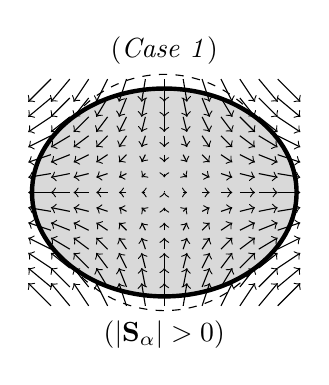
\begin{tikzpicture}[ultra thick,scale=0.6]
        \def\nRows{6}
        \def\nCols{6}
        \draw[dashed,thin] (0,0)circle(2.5);
        \draw[fill=gray!30] (0,0)ellipse(2.8 and 2.2);
        \foreach \x in {-\nRows,...,\nRows} {
            \foreach \y in {-\nCols,...,\nCols} {
                \pgfmathsetmacro\distance{veclen(\x*0.4, \y*0.4)};
                \pgfmathparse{\distance < 2.45 ? "blue" : "white"}
                \edef\colour{\pgfmathresult};
                \ifthenelse{\equal{\colour}{blue}}{                    
                    \draw[thin,->](\x*0.4,\y*0.4)--++(0.08*\x,-0.08*\y);
                }
            }
        }
        \node (txt) at (0,3){(\textit{Case 1})};
        \node (txt) at (0,-3){($|\textbf{S}_\alpha| > 0$)};
    \end{tikzpicture}
     \hfill
    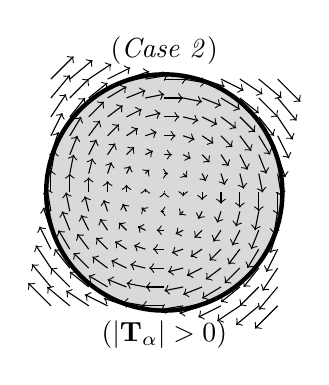
\begin{tikzpicture}[ultra thick,scale=0.6]
        \def\nRows{6}
        \def\nCols{6}
        \draw[fill=gray!30] (0,0)circle(2.5);
        \foreach \x in {-\nRows,...,\nRows} {
            \foreach \y in {-\nCols,...,\nCols} {
                \pgfmathsetmacro\distance{veclen(\x*0.4, \y*0.4)};
                \pgfmathparse{\distance < 2.5 ? "blue" : "white"}
                \edef\colour{\pgfmathresult};
                \ifthenelse{\equal{\colour}{blue}}{                    
                    \draw[thin,->](\x*0.4,\y*0.4)--++(0.08*\y,-0.08*\x);
                }
            }
        }
        \node (txt) at (0,3){(\textit{Case 2})};
        \node (txt) at (0,-3){($|\textbf{T}_\alpha| > 0$)};
    \end{tikzpicture}
    \hfill
    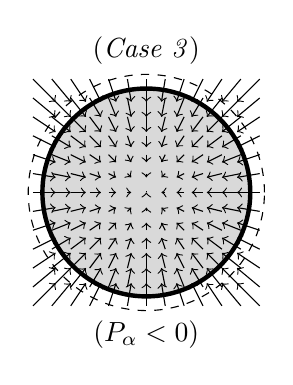
\begin{tikzpicture}[ultra thick,scale=0.6]
        \def\nRows{6}
        \def\nCols{6}
        \draw[dashed,thin] (0,0)circle(2.5);
        \draw[fill=gray!30] (0,0)circle(2.2);
        \foreach \x in {-\nRows,...,\nRows} {
            \foreach \y in {-\nCols,...,\nCols} {
                \pgfmathsetmacro\distance{veclen(\x*0.4, \y*0.4)};
                \pgfmathparse{\distance < 2.3 ? "blue" : "white"}
                \edef\colour{\pgfmathresult};
                \ifthenelse{\equal{\colour}{blue}}{                    
                    \draw[thin,->](\x*0.4,\y*0.4)--++(-0.08*\x,-0.08*\y);
                }
            }
        }
        \node (txt) at (0,3){(\textit{Case 3})};
        \node (txt) at (0,-3){($P_\alpha < 0$)};
    \end{tikzpicture}
    \hfill
    \caption{Graphical representation of the inner kinematics   of an arbitrary particle under three scenarios. 
        The arrows represent the velocity field inside the particle, $\textbf{w}_d^0$, with the corresponding value of the moment of momentum tensor indicated below. 
        The operator $|\ldots|$ refers to the norm of the tensors. 
        According to the inner velocity field:
        (\textit{Case 1}) The particle experiences a mean deformation, resulting in non-zero stretching of momentum along the principal axis of deformation;
        (\textit{Case 2}) The particle is rotating, leading to a non-zero angular momentum vector in the direction of rotation;
        (\textit{Case 3}) The particle undergoes compression, resulting in a negative trace of the moment of momentum.
    }
    \label{eq:scheme}
\end{figure}
Injecting, $f_d^0 = \rho_d$ in the second-order moment equation (derived in \ref{ap:Moments_equations}) we obtain,
%\JL{pq lequation du second moment de la masse ne fait pas intervenir la trace du premier moment de la qdm - cela semble incoherent ?}
\begin{equation}
    \ddt {\textbf{M}_\alpha}=2(\textbf{S}_\alpha+P_\alpha\bm\delta),
    \label{eq:dt_M_alpha}
\end{equation}
which is the second-order moment of mass conservation equation assuming that the fluid within the drop is divergence free. 
From \ref{eq:dt_M_alpha} we deduce that the evolution of the distribution of mass of a particle is solely determined by the  of momentum $\textbf{S}_\alpha$ and $P_\alpha$. 
This indicates that angular momentum does not influence the evolution of the second moment of mass, a consequence of the symmetry of the tensor $\textbf{M}_\alpha$, which must be preserved after differentiation with respect to time.
However, this does not imply that the particle angular velocity ($\bm\omega_\alpha$) does not appear in this equation. 
For instance, in the case of rigid body motion where $\textbf{w}_d^0 = \bm\omega_\alpha \times \textbf{r}$, we obtain the relation  $2(\textbf{S}_\alpha)_{ij} = \epsilon_{iab} (\bm\omega_\alpha)_a (\textbf{M}_\alpha)_{bj}+ 
\epsilon_{jab} (\bm\omega_\alpha)_a (\textbf{M}_\alpha)_{bi}  $. 

Now that we have described the kinematics   of the particle shape, let us proceed to derive an equation for the moment of momentum.
This equation is derived by injecting $\textbf{Q}_\alpha^{(1)} = \textbf{P}_\alpha$ in \ref{eq:dt_Q_alpha_tot}, it reads, 
\begin{equation}
    \ddt {\textbf{P}_\alpha}
    - \intO{ \rho_d  \textbf{w}_d^0 \textbf{w}_d^0 }
    = 
    - \intO{\bm{\sigma}_d^0}
    - \intS{ 
        \gamma (\bm\delta - \textbf{nn})
    }
    + \intS{ \textbf{r}\bm{\sigma}_f^0\cdot \textbf{n}}.
    \label{eq:dt_P_alpha}
\end{equation}
In the following sections the normal vector noted \textbf{n} always refer to $\textbf{n}_d$. 
The conservation equation of the angular momentum $\bm{\mu}_\alpha$ is obtained by taking the double contracted product of \ref{eq:dt_P_alpha} with $\bm\epsilon$, which directly gives
\begin{equation}
    \ddt\bm{\mu}_\alpha
    =  
    % \textbf{t}_\alpha.
    \intS{ \textbf{r} \times \bm{\sigma}_f^0\cdot \textbf{n} }
    \label{eq:dt_mu_alpha}
\end{equation}
Note that every term on the right-hand side of \ref{eq:dt_P_alpha} vanished due to their symmetric nature apart from the skew-symmetric part of the hydrodynamic stress, which is the hydrodynamic torque applied on the particle $\alpha$.
In particular, the surface tension terms do not appear in the angular momentum balance since the tensor $\bm\delta-\textbf{nn}$ is symmetric, which is consistent with the findings of \citet{hesla1993note}. 
As a consequence, the surface tension does not affect the angular momentum regardless of the particle shape. 
%In the literature, it is common to include the torque due to inter-particular interactions in the angular momentum balance, as is done in \citet{jackson1997locally} and \citet{zhang1997momentum}.
%In our case note that $\bm{\sigma}_f^0$ contains short-range hydrodynamic interaction forces. 

Taking the symmetric part of \ref{eq:dt_P_alpha}, and substrating the trace yields, 
\begin{align}
    &\ddt {\textbf{S}_\alpha}
    - \rho_d\intO{\left(\textbf{w}_d^0 \textbf{w}_d^0 -\frac{1}{3} (\textbf{w}_d^0 \cdot  \textbf{w}_d^0)\bm\delta\right)}
    = \nonumber \\
    &- 2\mu_d\intO{\textbf{e}_d^0}
    -  \intS{ \gamma
        \left( \frac{1}{3}\bm\delta - \textbf{nn} \right)
    }
    + \frac{1}{2}\intS{\left(\textbf{r}\bm\sigma_f^0+\bm\sigma_f^0\textbf{r}-\frac{2}{3}(\bm\sigma_f^0 \cdot \textbf{r})\bm\delta \right)\cdot \textbf{n}},
    \label{eq:dt_S_alpha}
\end{align}
%internal velocity kinetic energy. %$\intO{\rho_d\textbf{w}_d^0\textbf{w}_d^0 }$.
%On the left-hand side of \ref{eq:dt_S_alpha} we identify two inertial terms, i.e. the derivative of $\textbf{S}_\alpha$ and the stress induced by the product of internal velocity within the drop.
%The inertia of the particle is then balanced by the terms on the right-hand side of the equation, namely: 
%the volumic integral of the particle viscous stress; 
%the surface integral of the surface tension stress ; 
%and the first moment of the hydrodynamic stress tensor.
%A discussion regarding the physical implications of this equation is provided below. 
where we have introduced the rate of strain tensor for phase \( k \), defined as \( \mathbf{e}_k^0 = \frac{1}{2} (\grad \mathbf{u}_k^0 + ^\dagger \grad \mathbf{u}_k^0) \). 
Here $^\dagger$ represents the transpose operator. 
On the left-hand side of Equation~\ref{eq:dt_S_alpha}, two inertial contributions can be identified: the time derivative of $\mathbf{S}_\alpha$, and the stress arising from the product of internal velocity field within the droplet. 
These inertial effects are counterbalanced by the terms appearing on the right-hand side of the equation, which include: the volume integral of the particle viscous stress; the surface tension moment; and the first moment of the hydrodynamic force.
%\JL{a finaliser}
While surface tension effects do not influence the linear or angular momentum equations directly, they do impact the moment of momentum $\textbf{P}_\alpha$, specifically its symmetric part $\textbf{S}_\alpha$.
Consequently, surface tension influences the hydrodynamic behavior of a particle exclusively through its effect on $\textbf{S}_\alpha$, which is related to the shape of a particle represented by $\textbf{M}_\alpha$, via \ref{eq:dt_M_alpha}.
%Whether it is solid or fluid particles \ref{eq:dt_S_alpha} becomes particularly relevant for expressing the averaged stress within an inertial suspension in terms of Lagrangian properties, as discussed in the next chapter. 
%\JL{enlever la trace}
%Taking the symmetric part of \ref{eq:dt_P_alpha}, and making use of \ref{eq:dt_M_alpha}, yields a dynamical balance equation for $\textbf{M}_\alpha$, namely
Inserting \ref{eq:dt_S_alpha} in  \ref{eq:dt_M_alpha} yields,
%\JL{enlever la trace et reecrire la partie ci-dessous + donner la definition de $e_d$ qui n'est pas de defini avant.}
\begin{align}    
    &\frac{1}{2}\frac{d^2 (\textbf{M}_\alpha-\frac{1}{3}(\textbf{M}:\bm\delta)\bm\delta)}{dt^2}
    =  \rho_d\intO{\left(\textbf{w}_d^0 \textbf{w}_d^0 -\frac{1}{3} (\textbf{w}_d^0 \cdot  \textbf{w}_d^0)\right)}
    - 2\mu_d\intO{\textbf{e}_d^0} \nonumber\\
    &- \intS{\gamma  
        \left( \frac{1}{3}\bm\delta - \textbf{nn} \right)
    }
    + \frac{1}{2}\intS{\left(\textbf{r}\bm\sigma_f^0+\bm\sigma_f^0\textbf{r}-\frac{2}{3}(\bm\sigma_f^0 \cdot \textbf{r})\bm\delta \right)\cdot \textbf{n}}.
    \label{eq:dt2_M_alpha}
\end{align}
%On the left-hand side of \ref{eq:dt_S_alpha}, we recover the symmetric part of the inertial contributions. 
%In opposition to \ref{eq:dt_P_alpha} we could substitute the term $\ddt (\textbf{P}_\alpha+\textbf{P}_\alpha^\dagger)$ initially present in the equation by $\ddt^2 \textbf{M}_\alpha$ using \ref{eq:dt_M_alpha}. 
%\ref{eq:dt2_M_alpha} is a second-order partial differential equation for the second order mass moment characterizing the droplet shape.
%In other words, \ref{eq:dt2_M_alpha} must be interpreted as an equation for the shape of the particle, represented by the tensor $\textbf{M}_\alpha$. 
%Thus, on the right-hand side of \ref{eq:dt_S_alpha}, we identify the terms which favors deformation, including the inertia of the velocity field within the droplet as well as the traceless part of the first moment and the terms wwohc resis deformation incluidng the viscous resistance within the droplet and the surface tension.
\ref{eq:dt2_M_alpha} is a second-order differential equation governing the second-order mass moment that characterizes the droplet shape. 
In other words, it should be interpreted as an equation describing the droplet shape, represented by the traceless part of the tensor $\textbf{M}_\alpha$.
Accordingly, the right-hand side of \ref{eq:dt2_M_alpha} contains terms that promote deformation-such as the product of the internal velocity field and the traceless component of the first moment as well as terms that oppose deformation, including droplet internal viscous resistance and surface tension.
%One might also recognize that \ref{eq:dt2_M_alpha} is in fact an extension of \citet{batchelor1970stress} result, but with the consideration of the inertia of the particle.
\ref{eq:dt2_M_alpha} is particularly useful to compute the unknown internal stress within solid particles, in terms of surface integral, i.e. the first moment of the hydrodynamic force.
This relation plays a key role in expressing the bulk stress of a suspension and ultimately leads to the effective viscosity, once a closed-form expression for the average first moment is obtained \citep{batchelor1970stress}. 
In the inertial regime, and for solid particles, the tensors $\textbf{M}_\alpha$ and the internal velocity field $\textbf{w}_d^0$ are fully prescribed by the particle kinematics. 
As a result, in \ref{eq:dt2_M_alpha}, $\textbf{M}_\alpha$ and $\textbf{w}_d^0$ appear not as unknowns but rather as known source terms.
For spherical particles specifically, the inertial correction to the first force moment has been derived by \citet{hwang1989modeling} and  \citet{lhuillier1996contribution}.
%For the specific case of spherical particles \citet{hwang1989,lhuillier1996contribution} have derived this inertial correction.
%This relation is used to express the bulk stress of a suspension.
%It eventually leads to the computation of the famous Einstein equivalent viscosity, upon having a closed expression for the average of the first moment \citep{guazzelli2011}. 
%In the inertial case and for solid particle, the tensors $\textbf{M}_\alpha$ and the inner velocity field $\textbf{w}_d^0$ are fully determined by the particle kinematic, indicating that $\textbf{M}_\alpha$ and $\textbf{w}_d^0$ can be used in \ref{eq:dt_S_alpha} not as unknowns but as source terms. 
%Consequently, for solid particles, \ref{eq:dt_S_alpha} must be interpreted as a generalized equation for the undefined stress $\bm\sigma_d^0$ integrated on the volume of the particles.

%Note that if intead we had considered spherical particles composed of compressible fluid \ref{eq:dt2_M_alpha} transforms into the Rayleigh-Lamb-Plesset equation as demonstrated in \citep{danielcours}.


%In our case, only the external contribution $\intS{\textbf{r}\bm\sigma_f^0\cdot \textbf{n}}$ is responsible for the generation of angular momentum, see \ref{eq:dt_mu_alpha}.
%Taking the symmetric part of this tensor ultimately removes this contribution. 

%\begin{equation}
%    \intO{\bm{\sigma}_d^0}
%    + \intS{\gamma(\bm\delta - \textbf{nn})}
%    = \frac{1}{2}\intS{(\textbf{r}\bm\sigma_f^0+\bm\sigma_f^0\textbf{r})\cdot \textbf{n}},
%    \label{eq:Batchelor}
%\end{equation}

%In \ref{ap:Moments_equations} we show how to derive the higher-order moment of momentum equations, which can also be viewed as formulas for the higher moments of the internal particle stress distribution. 
%It is interesting to mention that in a recent study of \citet{dolata2021faxen} and \citet{zhou2020lamb} they make use of the first two moments of momentum equations hidden into another but equivalent form, valid in the Stokes flow regime. 








\subsection{Averaged momentum and mass conservation equations}



Let us now focus on the averaged momentum equation of the continuous phase. 
By applying \eqref{eq:dt_f_k} with $f_k = \rho_f$ and $\rho_f\textbf{u}_f$ we obtain the mass and momentum equation for the continuous phase under the two fluid formulation, 
\begin{align}
    (\pddt + \textbf{u}_f\cdot \grad)\textbf{u}_f&=-\phi_f \div \textbf{u}_f
    \label{eq:mass_init}\\
    \phi_f \rho_f(\pddt + \textbf{u}_f  \cdot \grad) \textbf{u}_f
    % +  \div \avg{\chi_f\rho_f \textbf{u}_f'\textbf{u}_f'}
    &= 
    \div [\phi_f \bm\sigma_f-  \avg{\chi_f\rho_f \textbf{u}_f'\textbf{u}_f'}]
    + \phi_f \rho_f \textbf{g}
    - \avg{\delta_\Gamma \bm\sigma_f\cdot \textbf{n}}.
    \label{eq:two_fluid_momentum_init}
\end{align} 
To obtain the hybrid formulation one can expand the final term on the right-hand side of \ref{eq:two_fluid_momentum_init} using the Taylor expansion provided in \ref{eq:f_exp}.  
However, before doing so, it is important to examine the term \( \phi_f \bm\sigma_f \), as it contains a non-closed contribution originating from the averaging of the strain rate tensor. %a contribution from the dispersed phase. 
Properly identifying and isolating this contribution is a necessary step prior to performing the Taylor expansion.
%Moreover, there

%one may use \ref{eq:f_exp} to taylor expand the last term on the right-hand side of \ref{eq:two_fluid_momentum_init}. 
%However, it is first important to discuss the form of the term $\phi_f\bm\sigma_f$ since a dispersed phase term, is hidden into it, hence it is important to identify this term before carrying out the Taylor expansion. 

%\subsection{Mean stress formulation and momentum transfer decomposition}
%\JL{bien expliquer quand et comment apparaissent les distinctions sur le choix de la contrainte moyenne. en particulier voir en dessous}

We begin by noting that $\phi_f\bm\sigma_f$ can be expressed in terms of the averaged fluid pressure $p_f$, and continuous phase averaged velocity ($\textbf{u}_f$), or bulk-averaged velocity ($\textbf{u} = \phi_f \textbf{u}_f + \phi_d \textbf{u}_d$).
Expressing $\bm\sigma_f$ as a function of $\textbf{u}_f$ instead of $\textbf{u}$ (or vice versa) leads to two distinct forms of the momentum equation, each associated with different formulations of the closure terms. 
We also review several alternative choices found in the literature (see also \citet{jackson2000, pahtz2025general} for an overview focused on solid particles), emphasizing that while all these formulations are mathematically equivalent, they give rise to different closure problems. 
We argue that one particular formulation is probably the most suitable, especially in light of the closure terms available in the literature for non-dilute flows.%especially in the context of existing closure models for non-dilute flows.
%Choosing to express $\bm\sigma_f$ as a function $\textbf{u}_f$ rather than $\textbf{u}$ and vice versa, results in two distinct forms of the momentum equation and two distinct formulations of the closure terms. 
%We also discuss the various other choice available on the literature (see also \citet{jackson2000,pathz2025} for a review for solid particles) explaining that there is all choice are perfectly equivalent but leads to a different closure problems.
%Our belief his that there is one formulation which is the most appropriate with respect to of the closure terms available in the litterature for non-dilute flow.
%Although this topic has been already discussed in the context of solid particles  we propose here to expose both formulations and discuss which of the two equivalent (but different) formulations is the most suited for multiphase flow modeling. 

%Because we believe this topic has not been discussed much for non-solid particles in the literature, we propose here to expose both formulations and discuss which of the two equivalent (but different) formulation is the most suited for multiphase flow modeling. 
%Because we believe this topic has not been discussed much in the literature for non-solid particles, 

First we introduce what we refer to as the \textit{mean Newtonian stress}, based either on the continuous phase averaged velocity $\textbf{u}_f$ or on the bulk velocity \textbf{u}, namely,
\begin{align}
    \bm\Sigma_f 
    &
    = -p_f \bm\delta + 2\mu_f \textbf{E}_f    
    %= -p_f \bm\delta + \mu_f [\grad \textbf{u}_f + (\grad \textbf{u}_f)^{\dagger}], 
    \label{eq:Sigma_f_average}
    \\
    \bm\Sigma &
    = -p_f\bm\delta + 2 \mu_f \textbf{E}
    %= -p_f \bm\delta + \mu_f [\grad \textbf{u} + (\grad \textbf{u})^{\dagger}],
    \label{eq:Sigma_average}
\end{align}
where $\textbf{E}_f = [\grad \textbf{u}_f + (\grad \textbf{u}_f)^{\dagger}]/2$ and $\textbf{E} =[\grad \textbf{u} + (\grad \textbf{u})^{\dagger}]/2$ represent the \textit{mean strain rate} tensor based either on $\textbf{u}_f$ or on \textbf{u}. 
Additionally the ensemble averaged stress $\phi_f \bm\sigma_f$ may be written as 
\begin{equation}
    \phi_f \bm\sigma_f = - \phi _f p_f \bm\delta + 2 \mu_ f \phi_f \textbf{e}_f
    \label{eq:sigma_average}
\end{equation}
where $\phi _f \textbf{e}_f = \avg{\chi _f \textbf{e}_f^0}$. 
%Moreover by definition the bulk stress tensor reads $\textbf{E} = \phi _f\textbf{e}_f + \phi_d \textbf{e}_d$.
Inserting \ref{eq:Sigma_f_average} and \ref{eq:Sigma_average} in  \ref{eq:sigma_average} yields
%Using the constitutive law of Newtonian fluids we find, 
\begin{align}
    \phi_f \bm\sigma_f 
    &=
    % - \phi_f p_f \bm\delta
    % + \phi_f \mu_f [\grad \textbf{u}_f  + (\grad \textbf{u}_f)^\dagger]
    % - \mu_f \avg{\delta_\Gamma( \textbf{u}_f'  \textbf{n} +  \textbf{n} \textbf{u}_f' )}
    % =
    \phi_f \bm\Sigma_f
    - \mu_f \avg{\delta_\Gamma( \textbf{u}_f'  \textbf{n} +  \textbf{n} \textbf{u}_f' )}
    \label{eq:stress_closure}\\
    \phi_f \bm\sigma_f 
    &=
    % - \phi_f p_f \bm\delta
    % + \mu_f [\grad \textbf{u}  + (\grad \textbf{u})^\dagger]
    % - 2\mu_f \phi_d \textbf{e}_d
    % =
    \phi_f \bm\Sigma
    - \avg{2\mu_f \chi_d \textbf{e}_d^*}
    \label{eq:stress_closure1}
\end{align}
where we have used the relations 
\begin{equation}
    \avg{\chi_f \grad \textbf{u}_f^0}
    = 
    \phi_f \grad  \textbf{u}_f
    + \avg{\delta_\Gamma \textbf{n}_f \textbf{u}_f'}
    \label{eq:first_rel}
\end{equation}
and
\begin{equation}
    %\avg{\chi_f \textbf{e}_f^0}
%    = 
%    \avg{\textbf{e}^0}
%    - \avg{\chi_d \textbf{e}_d^0}
\phi _f\textbf{e}_f
%    = 
%    \textbf{E}
%    - \avg{\chi_d \textbf{e}_d^0}
    = 
    \phi_f \textbf{E}
    - \avg{\chi_d \textbf{e}_d^*},
    \label{eq:sec_rel}
\end{equation}
to derive \ref{eq:stress_closure,eq:stress_closure1}, respectively. 
 %in most practical situations of interest.
%Note that \ref{eq:first_rel} remains true in the presence of non zero interfacial rate of strain, while \ref{eq:sec_rel} requires the condition that the bulk rate of strain reads $\textbf{E} = \phi _f\textbf{e}_f + \phi_d \textbf{e}_d$ \textit{i.e.} that there is no shear stress at the interface of the droplets, so that $\avg{\delta_\Gamma \textbf{e}_\Gamma^0}= 0$, which is true in most of the practical cases of interest. 
In \ref{eq:stress_closure1} we have introduced $\textbf{e}_d^* = \textbf{e}_d^0 - \textbf{E} = \grad (\textbf{u}_d^0-\textbf{u})+\grad (\textbf{u}_d^0-\textbf{u})^\dagger$ which is the droplet internal shear rate relative to the `bulk' shear rate \textbf{E}.
%While $\textbf{u}_f' = \textbf{u}_f^0 - \textbf{u}_f$ in \ref{eq:stress_closure}. 
It is worth noting that \ref{eq:first_rel} remains valid even when the interfacial rate of strain is nonzero. 
In contrast, \ref{eq:sec_rel} holds under the assumption that the bulk rate of strain satisfies $\textbf{E} = \phi_f \textbf{e}_f + \phi_d \textbf{e}_d$, \textit{i.e.} that $\avg{\delta_\Gamma \textbf{e}_\Gamma^0} = 0$. 
This condition is supposed to be met here because we did not consider interfacial viscosity\citep{nadim1996concise}.
%Before presenting the hybrid form of the continuous phase momentum equation, it is interesting to expose the classic two-fluid formulation using the stress formulation given by \ref{eq:stress_closure} in the first place. 
%Before introducing the hybrid form of the continuous phase momentum equation, it is useful to first present the classical two-fluid formulation, employing the stress formulation \ref{eq:stress_closure}.
The averaged momentum equation  employing the stress formulation \ref{eq:stress_closure} read, 
\begin{align}
    % (\pddt + \textbf{u}_f\cdot \grad)\textbf{u}_f&=-\phi_f \div \textbf{u}_f\\
    \phi_f \rho_f(\pddt + \textbf{u}_f  \cdot \grad) \textbf{u}_f
    % +  \div \avg{\chi_f\rho_f \textbf{u}_f'\textbf{u}_f'}
    &= \phi_f 
    \left(\div \bm{\Sigma}_f
    + \rho_f \textbf{g}\right)
    - \div 
    [\avg{\chi_f\rho_f \textbf{u}_f'\textbf{u}_f'}
    +\avg{\delta_\Gamma \mu_f( \textbf{u}_f'  \textbf{n} +  \textbf{n} \textbf{u}_f')}]
    - \avg{\delta_\Gamma \bm\sigma_f^{(1)}\cdot \textbf{n}},
    \label{eq:two_fluid_momentum}
\end{align}
where, $\bm\sigma_f^{(1)}=\bm\sigma_f^0 - \bm\Sigma_f$ which also reads %is the Newtonian stress evaluated at a point on an interface relative to the mean stress $\bm\Sigma_f$. 
\begin{equation}
\bm\sigma_f^{(1)} = -p_f'\bm\delta
+ \mu_f [
    \grad \textbf{u}_f'
    + ^\dagger \grad \textbf{u}_f']
    \label{eq:disturbance_stress1}
\end{equation} 
Likewise, using \ref{eq:stress_closure1} one may also derive another form of the momentum equation, namely,
\begin{equation}
    \phi_f \rho_f(\pddt + \textbf{u}_f  \cdot \grad) \textbf{u}_f
    % +  \div \avg{\chi_f\rho_f \textbf{u}_f'\textbf{u}_f'}
    = \phi_f 
    \left(\div \bm{\Sigma}
    + \rho_f \textbf{g}\right)
    - \div 
    [\avg{\chi_f\rho_f \textbf{u}_f'\textbf{u}_f'} + \avg{2\mu_f \chi_d \textbf{e}_d^*}]
    - \avg{\delta_\Gamma \bm\sigma_f^{(2)}\cdot \textbf{n}},
    \label{eq:two_fluid_momentum2}
\end{equation} 
where $\bm\sigma_f^{(2)}=\bm\sigma_f^0 - \bm\Sigma$. 
%This stress tensor corresponds to the Newtonian stress (relative to the mean pressure and velocity field) typically available in numerical or theoretical studies. 
It can be also expressed as, 
%Clearly, subtracting by $\bm\Sigma_f$ to the local stress at the interface leads to the expression 
\begin{equation}
    \bm\sigma_f^{(2)} 
    =
    -p_f'\bm\delta
    + \mu_f [
        \grad \textbf{u}_f^*
        + ^\dagger \grad \textbf{u}_f^*
    ]
    \label{eq:disturbance_stress2}
\end{equation}
where $\textbf{u}_f^*= \textbf{u}_f^0 - \textbf{u}$.
%which corresponds to the Newtonian stress at the surface of the droplets (relative to the mean pressure and velocity field) typically available in numerical or theoretical studies.
%Likewise, substituting the mean stress with $\bm\Sigma$ in \ref{eq:disturbance_stress} one obtain the same formula except than $\textbf{u}_f'\to \textbf{u}_f^0 - \textbf{u}$. 
%Hence, 
In both cases (\ref{eq:two_fluid_momentum} and \ref{eq:two_fluid_momentum2}) one has to compute the local stress relative to the averaged continuous phase motion or bulk phase motion. 
% Note that because $\div \textbf{u} = 0$ it may be more convenient to  
%Note the differences between the last term of formulation \ref{eq:stress_closure} and \ref{eq:stress_closure1}, is equal to, $\phi_f (\div \bm\Sigma_f - \div\bm\Sigma)$
%Hence, the transition from one formulation to the other is straightforward, it just requires adding or subtracting $\phi_f (\div \bm\Sigma_f - \div\bm\Sigma)$. 
%However it is worth noting the physicsical meaning og this term which also reads,
Note the difference between the last terms in formulations \ref{eq:stress_closure} and \ref{eq:stress_closure1}, which is given by $\phi_f \div (\bm\Sigma_f -\bm\Sigma)$.
The transition from one formulation to the other is straightforward and only requires the addition or subtraction of this term. 
However, it is important to recognize its physical significance.
This difference can be expressed explicitly as,
\begin{equation}
    \phi_f \div(\bm\Sigma_f - \bm\Sigma) = \mu_f \phi_f \div \left[\grad (\phi_d (\textbf{u}_f - \textbf{u}_d)) + \grad (\phi_d (\textbf{u}_f - \textbf{u}_d))^\dagger \right]
    \label{eq:diff_sigma1}
\end{equation}
where the decomposition 
\begin{equation}
\textbf{u} = \phi_f \textbf{u}_f + \phi_d \textbf{u}_d,
\label{eq:u_mean} 
\end{equation}
has been used in the derivation.
\ref{eq:diff_sigma1} reveals that the difference between the two formulations introduces a non-Newtonian stress term.
This non-Newtonian stress shares similarities with the second-order force moment closure \citep{jackson1997locally,zhang1997momentum}, and it is typically related to intrinsic convection in sedimentation processes \citep{lhuillier2022}.
Therefore, when addressing the closure problem, it is essential to treat each stress formulation carefully, as the inclusion or exclusion of this additional term can significantly impact the resulting model.
%Then, when considering the colsure problem one has to be carefull to properly consider each formulation of the stress differently as both formulation will resulst in adding or removing this term.
%between \ref{eq:def_sigma_eff_f} and \ref{eq:def_sigma_eff_f2}  plus the differences between the corresponding drag force terms, is exactly equal to, $\phi_f (\div \bm\Sigma_f - \div\bm\Sigma)$.
%\JL{il faut que tu m'expliques : quand je soustrais les forces j'obtiens $\phi (\div \bm\Sigma_f - \div\bm\Sigma)$. OK on soustrait juste le RHS par ailleurs je pense qu'il faut detailler cela, c'est un point important.}
%\JL{en particulier $\div \bm\Sigma_f - \div\bm\Sigma = \div \nabla u_f - u \propto u_r$  a expliciter en montrant le developpment limite}





%Even though, both stress decomposition and momentum formulations proposed here are equivalent, each formulation have advantages and drawback which we discuss below.  
Although the stress decomposition and momentum formulations proposed herein are mathematically equivalent, each presents distinct advantages and limitations, which we examine in detail below.
%Now let us discuss on the choic between $\bm\Sigma$ and $\bm\Sigma_f$. 
%At first sight, using \ref{eq:dt_uf} with the effective stress given by \ref{eq:def_sigma_eff_f}, seems more practical because we are solving for the field $\textbf{u}_f$ hence avoiding the need of \ref{eq:velocity_conservation}. 
First, we may observe that a simplification arises for \ref{eq:stress_closure1} in the case of solid particles, for which $\textbf{e}_d^0 = 0$.
As a result $\phi _f \bm \sigma _f = - \phi _f p_f \bm\delta + 2 \mu_ f \textbf{E}$ \citep{joseph1990ensemble,jackson2000}. %and $\avg{\chi_d \textbf{e}_d^*} = -\phi\bm\Sigma$. \JL{a montrer}
Owing to this simplification, the formulation based on $\bm\Sigma$ and the associated closure relation \eqref{eq:stress_closure1} makes it a good candidate to be used in practice for solid particles. %is frequently adopted in the literature \citep{jackson2000}, despite requiring the inclusion of the additional momentum conservation equation.
Second, employing \ref{eq:two_fluid_momentum} with \ref{eq:disturbance_stress1} may appear more convenient as the governing equations are directly formulated in terms of the fluid velocity field $\textbf{u}_f$, thereby circumventing the need to explicitly include an expansion for the bulk fluid velocity. %the following equation
%Because $\textbf{u}$ may be required by \ref{eq:stress_closure1}, one also need to solve the equation, 
%\eqref{eq:velocity_conservation}.
%On the other hand we note that for solid particles $\textbf{e}_d^0 = 0$ and $\avg{\chi_d \textbf{e}_d'} = -\bm\Sigma\phi$, because of this great simplification \ref{eq:stress_closure1} is often used \citep{jackson2000} even if it requires adding \ref{eq:velocity_conservation} in the system of equation.  
%\JL{Je comprends l'interet de cette simplification, mais il faur toujours avoir une exression pr $\textbf{E}$ donc pour $\textbf{u}$}
Third, there exists a conceptual reason for preferring the bulk stress $\bm\Sigma$ when deriving closure relations for non-dilute suspensions.  %involving the fluctuating stress $\bm\sigma_f'$. 
Specifically, because $\bm\sigma_f^{(2)}$ depends on the disturbance velocity $\textbf{u}_f^* = \textbf{u}_f^0 - \textbf{u}$, the averaged velocity $\textbf{u}$ naturally serves as the "far-field" or "undisturbed" velocity boundary condition in the conditionally averaged Navier-Stokes equations \citep{hinch1977averaged,fintzi2025}. %(as also emphasized in the context of this PhD study).
%But there is another reason for using the `bulk stress' $\bm\Sigma$ as a reference stress to compute the closure terms involving $\bm\sigma_f'$. 
%Indeed, since $\bm\sigma_f'$ requires $\textbf{u}_f' = \textbf{u}_f^0 - \textbf{u}$, then \textbf{u} becomes the `far field' or `undisturbed' velocity boundary condition far from the test particle in the conditionally averaged Navier-Stokes equations \tb{(+my phd)}.
%On another hand, one may note that all the available theoretical solutions considering the disturbance field of a particle embedded in a pure solvent or in an effective medium (which represents other particles' contribution) use a divergence free `background flow' as limiting condition \citep{kim1985modelling,hinch1977averaged}.
%Since $\div \textbf{u} =0$ we deduce that the velocity field used in most (if not all) theoretical problems correspond to \textbf{u}. 
%Therefore, the disturbance  stress computed in these problems is $\bm\sigma_f'= \bm\sigma_f^0 - \bm\Sigma$. 
Notably, most (if not all) existing theoretical solutions addressing the disturbance field generated by a particle embedded in a Newtonian solvent or in an effective medium - representing other particles contribution - use a divergence-free background velocity field as limiting boundary condition \citep{hinch1977averaged, kim1985modelling}. 
Since $\div \textbf{u} = 0$, it follows that the velocity field used in these theoretical study corresponds to $\textbf{u}$. 
Consequently, the disturbance stress derived in those studies is $\bm\sigma_f^{(2)} = \bm\sigma_f^0 - \bm\Sigma$.
In opposition, the stress decomposition based on $\bm\Sigma_f$, involves the fields $\textbf{u}_f$ which is not divergence free. 
Hence, this `far field' or `undisturbed' velocity boundary condition far from the test particle does not correspond to the usual boundary condition assumed in most of the theoretical problems. 
%In conclusion, it is important to note that \textbf{u} corresponds exactly to the `background velocity' fields used in most of the theoretical derivations.
%Hence, the resulting closure terms (drag forces, stresslet and higher moments) derived in these studies refer to the closures expressed in terms of $\bm\sigma_f^0 - \bm\Sigma$.
%In all case one can always express $\bm\Sigma_f$ in terms of $\bm\Sigma$ hence which formulation to use is not a fatality. 
%However, one must always be careful when asserting that a given formulation of the drag force, for example, is exactly equivalent to a closure term found in the literature, as there are multiple possible formulations  (either based on $\bm\Sigma_f$, $\bm\Sigma$, $\bm\sigma_f$ or even  $p_f \bm\delta$). 
%Note that the choices between $\bm\Sigma_f$ and $\bm\Sigma$ only matter if one consider a closure problem, in which $\phi \textbf{u}_f \neq \phi \textbf{u}$, hence accurate at $O(\phi^2)$ at least (such as in \citet{hinch1977averaged,kim1985modelling}). 
In conclusion, it is important to recognize that the vector field \(\textbf{u}\) corresponds precisely to the 'background velocity' typically employed in theoretical derivations. 
Consequently, the closure terms obtained in such analyses -such as the hydrodynamic forces, the stresslet, and higher-order moments- are formulated in terms of the difference \(\bm\sigma_f^0 - \bm\Sigma\).
Of course, it is always possible to express \(\bm\Sigma_f\) in terms of \(\bm\Sigma\) (see \ref{eq:diff_sigma1}), meaning that the choice of formulation remains free. 
Nevertheless, we must be cautious when claiming that a specific expression of, for example, the Faxen contribution to the force is exactly equivalent to a closure term reported in the literature especially for non-dilute suspension. 
%Multiple valid formulations exist, involving \(\bm\Sigma_f\), \(\bm\Sigma\), \(\bm\sigma_f\), or even the pressure tensor \(p_f \bm\delta\).
% It should also be noted that the distinction between $\bm\sigma_f^{(1)}$ and $\bm\sigma_f^{(2)}$ becomes relevant only in the context of closure problems accurate at \(O(\phi^2)\) or more\footnote{Indeed, because $\textbf{u} \phi = \textbf{u}_f\phi +O(\phi^2)$ the distinction between bulk or continuous phase averaged velocity field becomes irrelevant in the closure problem. }. 
% \JL{pas compris cette derniere phrase que je pense il faut enlever : on montre que la distinction joue deja pour le second moment des forces en regime dilue non ?}

% \JL{je n'ai pas compris le paragraphe suivant - je ne sais pas si il est necessaire desormais vu l'organisation actuelle ou on fait le developement en serie de Taylor plus tard}
% One can remark the similarities between the surface exchange terms expansion, and the multipole expansion used in microhydrodynamic that characterize the disturbance field caused by a body immersed in a stokes flow \citet{pozrikidis1992boundary,kim2013microhydrodynamics}. 
% Moreover, one can wonder which of the formulation, \ref{eq:def_sigma_eff_f2} or \ref{eq:def_sigma_eff_f}, contains what is called the `Stresslet' and the higher moments of force given by the multipole expansion used in microhydrodynamic ? \citep{pozrikidis1992boundary,kim2013microhydrodynamics}\footnote{Note that the first term in this expansion is the same whether we use \ref{eq:def_sigma_eff_f2} or \ref{eq:def_sigma_eff_f}}.   
% These moments are usually defined as the `extra stress above the value of the fluid law'\citep{hinch1977averaged}.
% Because we are not studying the `bulk' momentum equation this definition does not directly apply in our context. 
% However, note that \ref{eq:stress_closure1} involves the bulk velocity \textbf{u} which must be used in the bulk stress momentum equation.
% Hence, we can state that the resulting formulation based on \ref{eq:stress_closure1} and given by \ref{eq:def_sigma_eff_f2}, corresponds to the multipole expansion of microhydrodynamic. 
% \tb{not entirely sure but i think this is an important point }
% Thus, the symmetric part of the second term of \ref{eq:def_sigma_eff_f2} is exactly what is called the `Stresslet', while the skew-symmetric part represents the hydrodynamic torque applied on the droplets.
% The remaining terms of \ref{eq:def_sigma_eff_f2} represent the contribution of the second, third\ldots, and higher moments of hydrodynamic forces acted upon the droplets.  




%Additionally, because other stress decomposition have already been proposed in the literature we propose to discuss their advantages and draw back. 
%In the pioneering study of \citep{zhang1997momentum}, and in numerous articles that followed, the disturbance stress is defined as $\bm\sigma_f'= \bm\sigma_f^0 - \bm\sigma_f$ which is what we could call the ``intuitive'' definition. 
%However, note that using \ref{eq:stress_closure} one obtain that, 
Furthermore, given that various stress decomposition have already been introduced in the literature, we propose to examine their respective advantages and limitations. 
In the seminal work by \citet{zhang1997momentum}, as well as in numerous subsequent studies, the disturbance stress is defined as $\bm\sigma_f' = \bm\sigma_f^0 - \bm\sigma_f$, a formulation that may be regarded as the "intuitive" definition. 
However, it is important to note that, by employing Equation~\ref{eq:stress_closure}, one obtains
\begin{equation}
    \bm\sigma_f'
    = \bm \sigma _f ^{(1)}
%    -p_f'\bm\delta
%    + \mu_f [
%        \grad \textbf{u}_f'
%        + ^\dagger \grad \textbf{u}_f'
%    ]
    + \frac{\mu_f}{\phi_f} \avg{\delta_\Gamma( \textbf{u}_f'  \textbf{n} +  \textbf{n} \textbf{u}_f' )}
    \label{eq:stress_closure_zhang}
\end{equation}
%The first term on the rhight hand side of this expression correspond to the relative Newtonian stress usually integrated on the surface of a droplet or solid particle.
%The last term is a contribution related to the stress induced by the dispersed phase which normally appear in the effective stress expansion as shown below.
%To provide a better understanding of this term we assume that the suspension is made of solid particles $\textbf{e}_d = 0$.%for the following discussion 
The last term represents a contribution from the stress induced by the dispersed phase, as illustrated below. 
To better understand this term, we consider the case of a suspension composed of rigid solid particles, for which the strain rate tensor of the dispersed phase vanishes, i.e., $\textbf{e}_d = 0$.
%we remark that for solid particles . 
By subtracting \ref{eq:stress_closure} from \ref{eq:stress_closure1}, we directly obtain
\begin{equation}
    \avg{\delta_\Gamma (\textbf{n} \textbf{u}_f'+  \textbf{u}_f' \textbf{n})}
    = \textbf{E}_f - \textbf{E}
    - \phi_d \textbf{E}_f 
    =
    (\textbf{u}_f - \textbf{u}_d)\grad \phi_d + \grad \phi_d (\textbf{u}_f - \textbf{u}_d)   
    -  \phi [\grad \textbf{u}_d+ (\grad \textbf{u}_d)^\dagger ]. 
\end{equation} 
where we have used \ref{eq:u_mean}.
Therefore, at least in the case of solid particles, this term becomes non-zero whenever there are significant gradients in volume fraction and mean particle velocity. %, as in the recent study by \citet{wang2024effect}.
%Therefore, at least for solid particles, this term is non-zero as soon as there are non-negligible gradients of volume fraction and mean gradients of particle velocities as in the recent work of \citet{wang2024effect}. 
%This finding implies that, in the recent work of \citet{wang2024effect}, where decomposition is employed for the drag force, we assert that they have actually computed the integral of the first two terms of \ref{eq:sigma_explict}, while neglecting the final term. 
%We conclude that the commonly used decomposition of the drag force introduced by \citet{zhang1997momentum,jackson2000}, given by \ref{eq:general_partition}, requires adding the term  $\avg{\delta_\Gamma (\textbf{n} \textbf{u}_f'+  \textbf{u}_f' \textbf{n})}$ to the classical Newtonian stresses in the second term of \ref{eq:general_partition} and subtracting it in the mean drag force term (first term of \ref{eq:general_partition}). 
%Interestingly, \citet{wang2024effect}\footnote{
%    In this study the drag force is defined as the second term on the right-hand side of \ref{eq:drag_final} (see equation (3) of \citet{wang2024effect}).
%    They compute the drag force term using DNS by integrating $\bm\sigma_f^0$ over the particles surfaces, hence, assuming that $\bm\sigma_f=0$ (because there is no mean pressure gradient or velocity gradient).  
%    However, it is likely that the author overlooked the last term of \ref{eq:sigma_explict} which is non-zero \eqref{eq:closure_un_nu} in this specific scenario because $\grad \phi \neq 0$. 
%} specifically investigates the effect of the volume fraction gradient ($\grad \phi$) on the drag force. 
%\JL{a finaliser, rederiver la relation de Nico}
%Same comments apply if one consider \ref{eq:stress_closure1} in the above expression. 
%Hence, because $\bm\sigma_f$ already contains closure terms related to the dispersed phase, it appears to be prone to error to subtract the whole expression of $\bm\sigma_f$ from $\bm\sigma_f^0$.
The same observations hold if one considers expression \ref{eq:stress_closure1} in the analysis above. 
Since $\bm\sigma_f$ already includes closure contributions associated with the dispersed phase, directly subtracting the full expression of $\bm\sigma_f$ from $\bm\sigma_f^0$ can lead to inconsistencies unless the closure problem is handled with sufficient care. 
Note that the last term of \ref{eq:stress_closure_zhang} is proportional to the interface area concentration, hence it is at most of $O(\phi_d)$.
Thus, when integrating $\bm\sigma_f'$ on the interface of the droplets, the contribution from that term to the mean momentum exchange term is at most of $O(\phi_d^2)$. 
\JL{pas compris cette derniere phrase.}

Another commonly adopted approach in the literature is $\bm \sigma ^{(4)} = \bm \sigma _f ^0 - p_f\bm\delta$ \citep{simonin1996,lhuillier2009rheology,morel2015mathematical,guazzelli2018rheology}.
This definition leads to the expression
\begin{equation}
    \bm\sigma_f^{(4)}  = -p_f' \bm\delta + \mu_f (\grad \textbf{u}_f^0 + ^\dagger \grad \textbf{u}_f^0),
\end{equation}
which implies that the closure is based on the absolute local fluid velocity $\textbf{u}_f^0$, rather than the fluctuating component $\textbf{u}_f'$.
%Hence the closure are computed based on the absolute local velocity $\textbf{u}_f^0$ instead of $\textbf{u}_f'.
%or in the case with buoyant particles simply $\sigma ^{(4)} = \bm \sigma _f ^0 - \rho_f\bm\delta$ \citep{lhuillier}
%One may also consider using  instead of $\bm\sigma_f$, $\bm\Sigma_f$ or $\bm\Sigma$, as done in \citet{morel2015mathematical} (\tb{paper de daniel ou il fait ca ?}), in this case $\bm\sigma_f'  = -p_f' \bm\delta + \mu_f (\grad \textbf{u}_f^0 + ^\dagger \grad \textbf{u}_f^0)$, hence the closure are computed based on the absolute local velocity $\textbf{u}_f^0$ instead of $\textbf{u}_f'$.
Without going into the details, note that numerous closures are based on the reciprocal theorem formulation \citep{kim2013microhydrodynamics,stone2001inertial,raja2010inertial}. %, this includes the Faxen contribution to the drag force . %the expressions given by the famous Faxen laws. 
The closures (drag forces, stresslet etc... ) provided by the reciprocal theorem are by construction expressed in terms of the disturbance fields ($p_f'$,$\textbf{u}_f'$), because they must decay to zero far from the test particle. 
%Therefore, this last formulation may not be the most practical as well\footnote{
For example, the Faxen contribution to the drag force in the case of a spherical solid particle of radius $a$ is given by $\textbf{f} = \pi a^3 \mu_f \grad^2 \textbf{u}_f$. 
This formulation is obtained  by considering the contribution from the disturbance stress, $\bm\sigma ^{(1)}  = -p_f' \bm\delta + \mu_f (\grad \textbf{u}_f' + ^\dagger \grad \textbf{u}_f')$, which vanish far from the test particle. 
If one uses the formulation based on $\bm\sigma_f^{(4)}  = -p_f' \bm\delta + \mu_f (\grad \textbf{u}_f^0 + ^\dagger \grad \textbf{u}_f^0)$, the Faxen contribution to the drag force becomes $\textbf{f} = \pi a^3 \mu_f \grad^2 \textbf{u}_f + \frac{4\pi a^3}{3}\mu_f \grad^2 \textbf{u}_f$ where the second term is the contribution from the mean velocity field.
Although both formulations are equally valid, the second one appears to be less commonly used and could potentially lead to misinterpretations or inconsistencies if not carefully handled. 
%}. 



%Because of those remarks, we will use in the following the formulation based on $\bm \sigma^{(2)}$ i.e. \ref{eq:two_fluid_momentum2} since we believe this is a formulation less prone to errors when considering the closure problem. 
%Moreover this is the formulation used in the closure problem for non-dilute flows. 
%For simplicity we will denote $\bm \sigma^{(2)} = \bm \sigma ^{*}$ in the rest of the paper.
%since we are working at $O(\phi_d)$.
In light of these considerations, we adopt the formulation based on $\bm \sigma^{(2)}$-i.e., \ref{eq:two_fluid_momentum2}-for the remainder of this work, as it is less prone to errors when considering the closure problem. 
Furthermore, this formulation is commonly employed in the analysis of non-dilute flows. 
For simplicity, we will denote $\bm \sigma^{(2)}$ as $\bm \sigma^{*}$ throughout the rest of the paper.
%This will avoid the need for \ref{eq:velocity_conservation} in the system of equation. 
%\tb{on pourrait utiliser aussi lautre peut importe }
%\JL{finaliser la discussion sur le fait que $\Sigma$ est le moins prine to errors + more ealsily extendeable to non dilute fraction}
%The last two terms on the right-hand side of \ref{eq:two_fluid_momentum} can be further expanded into a Taylor series using \ref{eq:f_exp_delta}. 
%Doing so leads us to the hybrid formulation of the continuous phase momentum  equation %(i.e. \ref{eq:avg_hybrid_dt_chi_f} %with $f_f^0 = \textbf{u}_f^0\rho_f$), namely,
%This gives the hybrid formulation of the continuous phase momentum equation,
%\begin{align}
%    \phi_f \rho_f(\pddt + \textbf{u}_f  \cdot \grad) \textbf{u}_f
%    &= \phi_f 
%    \left(\div \bm{\Sigma}_f
%    + \rho_f \textbf{g}\right)
%    + \div \bm\sigma_f^{(1)\text{eff}}
%    - \pSavg{\bm\sigma_f^{(1)}\cdot \textbf{n}}, 
%    \label{eq:dt_uf}
%\end{align}
%where we introduced the effective stress, 
%\begin{align}
%    \bm{\sigma}^{(1)\text{eff}}_f 
%    &= 
%    - \avg{\chi_f\rho_f \textbf{u}_f'\textbf{u}_f'} 
%    + \pSavg{[\textbf{r}\bm\sigma^{(1)}_f\cdot \textbf{n} - \mu_f (\textbf{u}_f' \textbf{n} + \textbf{n} \textbf{u}_f')]}\nonumber\\
%    &- \div
%        \pSavg{[\frac{1}{2}\textbf{rr}\bm\sigma^{(1)}_f\cdot \textbf{n}- \mu_f\textbf{r} (\textbf{u}_f' \textbf{n} + \textbf{n} \textbf{u}_f')]}
%        + \grad\grad (\ldots)
%    \label{eq:def_sigma_eff_f}
%\end{align}
%\JL{a finaliser}
The last two terms on the right-hand side of \ref{eq:two_fluid_momentum2} can be further expanded into a Taylor series using \ref{eq:f_exp_delta}.
Doing so leads us to the hybrid formulation of the continuous phase momentum  equation, %a relation similar to \ref{eq:dt_uf} except that $\bm\Sigma_f$ is replaced by $\bm\Sigma$, $\pSavg{\bm\sigma_f^{(1)}\cdot \textbf{n}}$ by $\pSavg{\bm\sigma_f^{(2)}\cdot \textbf{n}}$ and the effective stress $\bm\sigma_f^\text{(1)eff}$ by the tensor
\begin{align}
    \phi_f \rho_f(\pddt + \textbf{u}_f  \cdot \grad) \textbf{u}_f
    &= \phi_f 
    \left(\div \bm{\Sigma}
    + \rho_f \textbf{g}\right)
    + \div \bm\sigma_f^{\text{eff}}
    - \pSavg{\bm\sigma_f^{*}\cdot \textbf{n}}, 
    \label{eq:dt_uf2}
\end{align}
where,
\begin{align}
    \bm{\sigma}^{\text{eff}} 
    &= 
    - \avg{\chi_f\rho_f \textbf{u}_f'\textbf{u}_f'} 
    + \pavg{\intS{\textbf{r}\bm\sigma^{*}_f\cdot \textbf{n}} - \delta_p\intO{2\mu_f\textbf{e}_d^*}}\nonumber\\
    &- \div
        \pavg{ \frac{1}{2}\intS{\textbf{rr}\bm\sigma^{*}_f\cdot \textbf{n}}
        - \delta_p\intO{2\mu_f \textbf{r} \textbf{e}_d^*}}
        + \grad\grad (\ldots). 
    \label{eq:def_sigma_eff_f2}
\end{align}
Under this form, the left-hand side of \ref{eq:dt_uf2} represents the total derivative of $\textbf{u}_f$, while on the right-hand side we find: (1) the mean Newtonian stress contribution based on the bulk velocity $\bm\Sigma$, (2) the mean buoyancy force, (3) the Reynolds stress term, and (4) the moments of momentum exchange terms, which are computed based on $\bm\sigma_f^*$.
The $(\ldots)$ refers to the higher order moments. 
% The last term correspond to the mean hydrodynamic force on the particles.
%\JL{il faut mettre les closure pr connaitre les ordres de grandeurs.}
%In this formulation it is implied that $\bm\sigma_f'$ is given by $\bm\sigma_f' = \bm\sigma_f^0 -\bm\Sigma$.

The averaged mass of droplets ($m_p$), the averaged center of mass velocity ($\textbf{u}_p$), the averaged second moment of mass ($\textbf{M}_p$), and the averaged first moment of momentum ($\textbf{P}_p$), 
% are defined as,
% \begin{align}
%     n_p m_p 
%     =
%     \pOavg{\rho_d},
%     && n_p m_p \textbf{u}_p  
%     =
%     \pOavg{\rho_d \textbf{u}_d^0}\\
%     n_p \textbf{M}_p  
%     =
%     \pOavg{\rho_d \textbf{rr} },
%     && n_p \textbf{P}_p  
%     =
%     \pOavg{\rho_d \textbf{r} \textbf{u}_d^0},
% \end{align} 
% respectively.
% All the quantities defined above 
obey conservation laws that are given according to \ref{eq:avg_hybrid_q}, \ref{eq:avg_hybrid_q_1} and \ref{eq:avg_hybrid_q_n} (for conservation laws at the local scale, refer to the previous section.).
They read, 
%\JL{pq lequation du second moment de la masse ne fait pas intervenir la trace du premier moment de la qdm - cela semble incoherent ? OK car on est en incompressible}
%\JL{attention il manque des primes sur certaines variables}
\begin{align}
    (\pddt + \textbf{u}_p \cdot \grad)n_p
    &=
    - n_p \div \textbf{u}_p\label{eq:mass_p}\\
    n_p (\pddt + \textbf{u}_p \cdot \grad) \textbf{M}_p
    +\div  \pavg{\textbf{u}_\alpha'\textbf{M}_\alpha}
    &=
    n_p2  (\textbf{S}_p+P_p\bm\delta)
    \label{eq:dt_hybrid_Mp}\\
    \label{eq:dt_hybrid_up}
    m_p n_p(\pddt + \textbf{u}_p \cdot \grad)\textbf{u}_p
    + \div \pavg{m_p \textbf{u}_\alpha'\textbf{u}_\alpha'}
    &=
    m_p n_p \textbf{g}
    %+ \pSavg{\bm\sigma_f^0 \cdot \textbf{n}}\\
    + \pSavg{\bm\sigma_f^* \cdot \textbf{n}} + \pSavg{\bm\Sigma \cdot \textbf{n}}\\
    \label{eq:dt_hybrid_mup}
    n_p (\pddt + \textbf{u}_p \cdot \grad) \bm{\mu}_p
    +\div  \pavg{\textbf{u}_\alpha'\bm\mu_\alpha}
    &=
    \pSavg{\textbf{r}\times(\bm\sigma_f^*\cdot \textbf{n})}
    \\
    % \color{red}
    n_p (\pddt + \textbf{u}_p \cdot \grad) \textbf{S}_p
    +\div  \pavg{\textbf{u}_\alpha'\textbf{S}_\alpha}
    &=
    \rho_d \pOavg{
        \textbf{w}_d^0  \textbf{w}_d^0 
        -\frac{1}{3} (\textbf{w}_d^0 \cdot  \textbf{w}_d^0) \bm\delta
    }
    - \pOavg{2 \mu_d\textbf{e}_d^*} \nonumber \\
    &+\pSavg{\frac{1}{2}(\textbf{r}\bm\sigma_f^*+^\dagger\textbf{r}\bm\sigma_f^*-\frac{2}{3}(\bm\sigma_f^* \cdot \textbf{r})\bm\delta)\cdot \textbf{n}}\nonumber\\
    &-  \pSavg{\gamma (\frac{1}{3}\bm\delta - \textbf{nn})}
     + (1-\lambda)\pOavg{2\mu_f\textbf{E}}\nonumber \\
     &+ \frac{1}{2}\pOavg{\textbf{r}(\div\bm\Sigma)+ (\div\bm\Sigma) \textbf{r}},
    \label{eq:dt_hybrid_Sp}
\end{align}
% \JL{j'ai mis la derniere equation en rouge car n'arrivant pas à la demontrer je ne suis pas sur du second membre. par ailleurs il y avait des petites coquilles dans les autres équations que j'ai corrigé. je te laisse regarder si jamais tu en vois d'autres}
%\JL{discuter du lien avec Curtiss (equations pour les particules non spheriques). en particlier ne ne pense pas que lequation de $S_p$ soit necessaire}
%The above system of equations is a generalization of the averaged equations for non-spherical particles \citep{curtiss1956kinetic}. 
%One may note that for solid particles \ref{eq:dt_hybrid_Sp} is useless as $\textbf{S}_p$ can be expressed  as a function of $\textbf{M}_p$ and $\bm{\mu}_p$ and correlation between their fluctutations. 
% where $\textbf{S}_p$ is the mean symmetric traceless part of $\textbf{P}_p $ and $\mu_p$ the mean angular momentum.% have respectively 
The presented system of equations extends the averaged equations developed for non-spherical solid particles \citep{curtiss1956kinetic}. 
It is worth noting that, in the case of solid particles, \ref{eq:dt_hybrid_Sp} becomes redundant, as the tensor $\textbf{S}_p$ can be expressed in terms of $\textbf{M}_p$, $\bm{\mu}_p$ or the mean angular velocity, and the correlations of their fluctuations.
In this case, \ref{eq:dt_hybrid_Sp} must be solved to determine the unknown internal stress of the solid particles. 
%In these equations we have introduced the rate of strain tensor $\textbf{e}_k^0 = 1/2 (\grad \textbf{u}_k^0 + \grad \textbf{u}_k^0)$. %as the local shear rate of phase $k$.
%It is now clear that if the surface tension forces play no role in the linear and angular momentum equation, however, it impacts the moment of momentum $\textbf{P}_\alpha$ or more specifically its symmetric part $\textbf{S}_\alpha$.
%Thus, the surface tension force impacts the hydrodynamic behavior of a particle solely through its action on $\textbf{S}_\alpha$, which is related to the shape of a particle represented by $\textbf{M}_\alpha$, through \ref{eq:dt_M_alpha}.
%In \ref{ap:Moments_equations} we show how to derive the higher-order moment of momentum equations, which can also be viewed as formulas for the higher moments of the internal particle stress distribution. 
%It is interesting to mention that in a recent study of \citet{dolata2021faxen} and \citet{zhou2020lamb} they make use of the first two moments of momentum equations hidden into another but equivalent form, valid in the Stokes flow regime. 
%Although surface tension effects do not directly influence the linear or angular momentum equations, they impact the moment of momentum \( \mathbf{P}_\alpha \), and more specifically, its symmetric component \( \mathbf{S}_\alpha \).
%Consequently, the impact of surface tension on the hydrodynamic behavior of a particle manifests exclusively through its contribution to \( \mathbf{S}_\alpha \). 
%This quantity is related to the particle shape, represented by \( \mathbf{M}_\alpha \), via \ref{eq:dt_M_alpha}.
In \ref{ap:Moments_equations}, we detail the derivation of higher-order moment of momentum equations, which can also be interpreted as expressions for the higher moments of particles internal stress distribution. 
% Notably, recent works by \citet{dolata2021faxen} and \citet{zhou2020lamb} have employed the first two moment equations in an alternative but equivalent form, valid in the Stokes flow regime.
% \JL{pas compris la comparaison avec les travaux de Dolata et Zhou qui pour moi considerent les moments des forces ?}
% In these expressions we partitioned the local hydrodynamic stress $\bm\sigma_f^0$ and $\bm\sigma_d^0$, into their fluctuating parts, $\bm\sigma_f'=\bm\sigma_f^0 - \bm\Sigma_f$,  $\bm\sigma_d' = \bm\sigma_d^0 + p_f\bm\delta - 2\mu_d \textbf{E}_f$ and mean parts $\bm\Sigma_f$ and $-p_f \bm\delta + 2\mu_d \textbf{E}_f$, respectively. 
% Note that one can also write these equations in terms of $\bm\Sigma$ and $\textbf{E}$, the only requirement being that the exchange terms of \ref{eq:dt_hybrid_Mp} to \ref{eq:dt_hybrid_Sp} must correspond to the exchange terms used in the continuous phase momentum conservation \eqref{eq:dt_uf} (with \ref{eq:def_sigma_eff_f} or \ref{eq:def_sigma_eff_f2}). 

The set of equations \ref{eq:mass_init}, \ref{eq:dt_uf2}, \ref{eq:mass_p}-\ref{eq:dt_hybrid_Sp} is completed by the following relations %condition on the total volume conservation which reads, 
\begin{align}
    \phi_f + \phi_d &= 
    \phi_f + \phi  + \frac{1}{2}\grad\grad : (\textbf{M}_p n_p) + \ldots = 1,
    \label{eq:volume_conservation}\\
    \textbf{u} &= \textbf{u}_f\phi_f + 
    \phi\textbf{u}_p - \frac{1}{\rho_d} \div  (\textbf{P}_p n_p) + \ldots
    \label{eq:velocity_conservation}
\end{align}
where we have introduced the notation $\phi = n_pv_p$. 
\ref{eq:velocity_conservation} is obtained by inserting expansion \ref{eq:f_exp_chi} in \ref{eq:u_mean}.

\subsection{Symmetry of the effective stress tensor}
%\JL{specifier que l'on parle bien des contraintes eqs cote fluide.}
We remark that the second moment and higher-order moments in \ref{eq:def_sigma_eff_f2} appear under two divergence operators in \ref{eq:dt_uf2}. 
Hence, if we note $\Sigma_{ijk}$ the third rank tensor that represent these moments, then only the vector $\partial_k \partial_j\Sigma_{ijk}$ is of physical significance in the momentum balance \eqref{eq:dt_uf2}.
Thus, one can demonstrate that \citep{lhuillier1996contribution}
\begin{equation}
    \partial_j \partial_k \Sigma_{ijk}
    = \partial_j \partial_k \Sigma_{i(jk)}
    =
    \partial_j \partial_k \left[
        \Sigma_{i(jk)}
        + \Sigma_{j(ik)}
        - \Sigma_{k(ij)}
    \right],
    \label{eq:sym_proof}
\end{equation}
where $\Sigma_{i(jk)} = \frac{1}{2}[\Sigma_{ijk} + \Sigma_{ikj}]$ represents the symmetric part of $\Sigma_{ijk}$ over the index $jk$, as indicated by the parenthesis (and so on for the other tensor). 
This expression is allowed because $\partial_j \partial_k (\Sigma_{ijk} - \Sigma_{ikj}) = 0$ and $\partial_j \partial_k (\Sigma_{j(ik)} - \Sigma_{k(ij)}) = 0$. 
This manipulation highlight the fact that the effective stress due to the second order moments remains symmetric over the indices $ij$, in all circumstances.
Hence, as already demonstrated by \citet{lhuillier1996contribution} only the hydrodynamic torque can induce skew-symmetric stresses in the effective stress of the averaged momentum equation. 



\section{Closure for dilute suspensions of droplets in viscous dominated flows}
\label{sec:closure}
We now consider the closures for a dilute, monodisperse suspension of spherical droplets with radius $a$ in Stokes flow. %, in the absence of mass transfer. 
Our analysis reproduces the results of \citet[Appendix B]{zhang1997momentum} concerning the form of the closure terms associated with relative motions between phases, ($\textbf{u}_p, \textbf{u}, \textbf{E}\ldots$). 
In addition, we provide explicit expressions for these closure terms in terms of $\grad\gamma$ and higher derivatives. 

The closure terms in the above set of equation are expressed in terms of $p_f'$ and $\textbf{u}_f^*$, therefore we are seeking for the disturbance velocity and pressure fields generated by a spherical droplet immersed in an arbitrary flow. 
Specifically, the fields $(\textbf{u}_f^*,p_f')$ correspond to the solution of the 
 \textit{single-particle conditionally averaged} Navier-Stokes equations \citep{hinch1977averaged,zhang1994averaged,fintzi2025}. 
Note that to obtain averaged equations accurate at $O(\phi)$, it is sufficient to consider a closure problem accurate at $O(1)$  in $\phi$ \citep{hinch1977averaged,zhang1994averaged}, hence neglecting droplets interactions.
Additionally, we neglect inertia in the closure problem, meaning that we neglect all the terms of $O(Re)$ in the closure problem, and all the term of $O(Re\phi)$ in the averaged equations. 
Finally, even though we consider surface tension gradient, we consider in the first place spherical droplets hence neglecting all the term of order $O(Ca)$ in the closure problem. 
Consequently, we consider an isolated spherical droplet translating in an arbitrary Stokes flow with stresses jumps at the interfaces.
The solution for this problem can be found in many studies in the literature, including \citet{
    Subramanian_1985,
    nadim1991motion,
    pozrikidis1992boundary,leal2007advanced,raja2010inertial,pozrikidis2011introduction,kim2013microhydrodynamics}, this will enable us to compute the closure terms.
For ease of understanding we have exposed the closure problem, and its solutions, in \ref{ap:singularity_solution}. 


Here, $L$ denotes the characteristic length scale over which the averaged quantities may vary \citep{jackson1997locally}. 
Each averaged property may possess a different variation length scale.
For instance, consider $\grad \textbf{u}$ which typically varies at the length scale of the process, whereas $\grad\gamma$ may vary over a smaller length scale. 
For example, if the gradient of surface tension is generated by the transport of surfactants, it typically varies over a length scale of the drop size. 
If $\gamma$ varies due to a non-constant temperature field, the length scale of variation will correspond to that of the temperature field, which is related to the process or macro scale. 
To simplify the problem, we assume that $\grad\gamma$, and $\grad \textbf{u}$ typically vary on the order of $\sim L$. 
Then, we consider all contributions proportional to $O(a^2/L^2)$ to be negligible in the averaged equations \citep{jackson1997locally,zhang1997momentum}. 


A summary of the dimensionless parameters is presented in \ref{tab:dimensionless_para}. 
% \tb{ 
% We also address the closure of the various covariance terms arising in the averaged equations.}


\subsection{Hydrodynamic stresses closures}


\begin{table}
    \centering
\begin{tabular}{|c|c|}\hline
    Velocity scale & $U$ \\
    Macroscopic length scale & $L$ \\
    Droplets radius & $a$ \\
    Reynolds number & $Re = \rho_f a U / \mu_f$   \\
    Capillary number & $Ca = \mu_f U / \gamma$ \\
    Marangoni number & $Ma =  a|\grad\gamma| / \mu_f U$ \\\hline
Viscosity ratio & $\lambda = \mu_d / \mu_f$ \\
Density ratio & $\zeta = \rho_d / \rho_f$ \\
\hline
    \end{tabular}
    \caption{Definition of physical quantities and dimensionless parameters.
    Note that the choice of velocity scales depends on the specific problem under consideration. 
    For example, in the case of sedimenting droplets in a quiescent fluid, the characteristic velocity is typically $U \sim |\textbf{u}_p|$.}
    \label{tab:dimensionless_para}
\end{table}



%\subsubsection{Hydrodynamic stresses closures at $O(\phi Re^0 Ca^0)$}
%\JL{pq la partie antisymetrique du premier moment est nulle ?}
In the first place we focus on the surface exchange terms. 
We may directly compute the following expressions from the singularity solutions and find\footnote{
    We follow the convention of \citet{happel2012low} for the transpose operator.
    For an arbitrary order tensor \textbf{A}, its transpose is denoted either as $^\dagger A_{ijkl\ldots} = A_{jikl\ldots}$ or as $ (A_{\ldots ijkl})^\dagger = A_{\ldots ijlk}$}, 
\begin{align}
    \pSavg{\bm\sigma_f^*\cdot \textbf{n}} &
    =
    \phi
    \frac{\mu_f}{a^2}
    \frac{3(2+3\lambda)}{2(1+\lambda)}\textbf{u}_r
    + \phi\mu_f  \frac{3\lambda}{4(\lambda +1)} \grad^2 \textbf{u}% \nonumber\\
    + \phi \frac{1}{a}\frac{1}{\lambda +1} \grad \gamma
    + \phi a \frac{1}{10(\lambda +1)}\grad^2(\grad\gamma)
    \label{eq:drag_forces}
    \\
    \pSavg{\textbf{r}\bm\sigma_f^*\cdot \textbf{n}} &
    = \mu_f \phi 
    \frac{3(5\lambda +2)}{5(\lambda +1)}\textbf{E}
    + \mu_f a^2 \phi \frac{3\lambda}{10(\lambda+1)}\grad^2  \textbf{E}
    + \phi a \frac{9}{25(\lambda +1)}(\grad\grad \gamma- \bm\delta\grad^2 \gamma/3)
    % - \phi a \frac{3}{25(\lambda +1)}\bm\delta\grad^2 \gamma
    \\
    \pSavg{\textbf{rr}\bm\sigma_f^*\cdot \textbf{n}} &
    =
    \mu_f \phi \frac{3}{5(\lambda +1)} (\textbf{u}_r \bm\delta + ^\dagger\textbf{u}_r\bm\delta )
    + \mu_f \phi \frac{3(5\lambda +2)}{10(\lambda+1)}\bm\delta \textbf{u}_r\nonumber\\
    &
    - \phi a\frac{2}{5(\lambda+1)}(\grad \gamma \bm\delta+  ^\dagger \grad \gamma\bm\delta)
    + \phi a\frac{3}{5(\lambda+1)} \bm\delta \grad \gamma
    % higher orders
    % &+ a^2 \mu_f \phi \frac{119\lambda^2+190\lambda-24}{140(\lambda+1)(\lambda+4)}(\grad\grad \textbf{u})_{jki}
    % + a^2\mu_f \phi \frac{7\lambda^2+190\lambda+88}{140(\lambda+1)(\lambda+4)}\grad(\grad \textbf{u}+\grad \textbf{u}^\dagger )_{ijk}\nonumber\\
    % &+a^2\mu_f \phi \frac{13\lambda - 4 }{14(\lambda+1)(\lambda+4)}\grad^2 ( \textbf{u}\bm\delta)_{ijk}
    % - a^2\mu_f \phi \frac{7\lambda^2 + 80 \lambda - 72}{140(\lambda+1)(\lambda+4)}\grad^2(\textbf{u}\bm\delta  + \textbf{u}_f \bm\delta)_{jki}\nonumber \\
    % \pSavg{\textbf{rrr}\bm\sigma_f'\cdot \textbf{n}} &
    % =
    % a^2\phi\frac{4}{105}\frac{21\lambda+2}{\lambda+1}
    % (\textbf{E}\bm\delta+\textbf{E}\bm\delta + \textbf{E}\bm\delta)
    % + 
    % a^2\phi \frac{64}{105(\lambda+1)}
    % (\bm\delta\textbf{E}+\bm\delta\textbf{E} + \bm\delta\textbf{E})
\end{align}
\begin{align}
    \pSavg{ 2\mu_f \textbf{e}_d^*}
    &=
    -  \mu_f \phi \frac{2(5\lambda +2)}{5(\lambda+1)}\textbf{E}
    -  a^2 \mu_f \phi \frac{3\lambda}{15(\lambda+1)}\grad^2  \textbf{E}
    - \phi a  \frac{6}{25(\lambda+1)} (\grad\grad \gamma- \bm\delta\grad^2 \gamma§/3)\\
    \pSavg{ 2 \mu_f \textbf{re}_d^* }
    &=
    \phi \frac{3\pi}{10(\lambda+1)}
    (\bm\delta \textbf{u}_r +  \bm\delta\textbf{u}_r^\dagger)
    -\phi \frac{\pi}{5(\lambda+1)}\textbf{u}_r\bm\delta \\
    % maragra
    &-\phi a\frac{1}{5(\lambda+1)} (\bm\delta \grad \gamma+ \bm\delta\grad\gamma^\dagger)
    + \phi a\frac{2}{15(\lambda+1)}\grad\gamma\bm\delta 
    % ohther
    % &-  a^2 \phi \frac{2(2\lambda+1)}{7(\lambda+1)(\lambda+4)}(\grad\grad \textbf{u}_f)_{ijk}
    % - a^2 \phi \frac{7\lambda^2+20\lambda+3}{35(\lambda+1)(\lambda+4)}\grad(\grad \textbf{u}_f+\grad \textbf{u}_f)_{kij}\nonumber\\
    % &+ a^2 \phi \frac{3\lambda-2}{14(\lambda+1)(\lambda+4)}\grad^2(\bm\delta\textbf{u}_f)_{ijk}
    % -  a^2 \phi \frac{14\lambda^2+75\lambda+6}{140(\lambda+1)(\lambda+4)}\grad^2 (\textbf{u}_f \bm\delta + \textbf{u}_f \bm\delta)_{ijk}\nonumber
    \label{eq:secondUN}
    % \pSavg{ \textbf{rr}_{mq}(\textbf{n} \textbf{u}_f' + \textbf{u}_f' \textbf{n})_{iv}}
    % &=
    % -\phi a^2 \frac{4(7\lambda+4)}{105(\lambda+1)}
    % (\textbf{E}_{im} \bm\delta_{qv}
    % +\textbf{E}_{iq}\bm\delta_{mv}
    % + \textbf{E}_{mv} \bm\delta_{iq}
    % + \textbf{E}_{qv}\bm\delta_{im}
    % )
    % \\
    % &
    % -\phi a^2 
    % \frac{16}{105(\lambda+1)}(\textbf{E}_{mq}\bm\delta_{iv})
    % -\phi a^2 \frac{8(7\lambda+2)}{105(\lambda+1)}\textbf{E}_{iv}\bm\delta_{mq}
    % \label{eq:thirsmom}
\end{align}
where we have introduced the relative velocity $\textbf{u}_r = \textbf{u} - \textbf{u}_p$, and the viscosity ratio $\lambda = \mu_d/\mu_f$. 
Most of the terms $\propto \textbf{E}$, or $\propto \textbf{u}_r$ in this expression are already well known and will not be discussed here.  
In \ref{eq:drag_forces} the third term represents the force induced by $\grad \gamma$, which drives the thermocapillary migration of droplets for example if one relates $\grad\gamma$ to temperature gradient.  
The last term of \ref{eq:drag_forces} corresponds to a ``Faxen-like'' contribution of the Marangoni forces and involves the third derivative $\gamma$.
It is worth noting that the first moments scale as $\propto \phi \grad\grad \gamma$, while the second moments scale as $\propto \phi \bm\delta \grad \gamma$.
These scaling could have been anticipated based on symmetry considerations. 
Note that we have neglected the terms proportional to $\grad^2 \textbf{E}$ in the first moment expression, and to $\grad\grad \textbf{u}$ or $\grad\grad\grad \gamma$ in the second moment expression, as they are of order $O(a^2/L^2)$ or smaller.
The complete expressions for the first and second moments, including these higher-order contributions, are provided in \ref{ap:singularity_solution}.

The above closure just provide the contribution from the disturbance fields, however in the dispersed phase relations \eqref{eq:dt_hybrid_up,eq:dt_hybrid_Sp} one need the contribution from the the total momentum exchange including the contribution of the mean stress $\bm\Sigma$. 
These terms can easliy be obtain following the procedure outlined in \citep{zhang1997momentum,morel2015mathematical}, and reads, 
\begin{align}
    \pSavg{\bm\Sigma\cdot \textbf{n}}
    &= \phi\div\bm\Sigma + O(a^2/L^2),\\
    \pOavg{\textbf{E}}
    &= \phi \textbf{E}+ O(a^2/L^2),\\
    \pSavg{\textbf{r}(\div \bm\Sigma)}
    &= O(a^2/L^2). 
    \label{eq:mean_contributions}
\end{align}
We have used the approximation of $\bm\Sigma_f(\textbf{x}+\textbf{r}) = \bm\Sigma_f(\textbf{x}) + \textbf{r}\cdot\grad \bm\Sigma_f|_{\textbf{r}=0} + \ldots$ and neglected the $O(a^2/L^2)$ terms. 


\subsection{Velocity variance and covariance closures}


The disturbance velocity field $\textbf{u}_f'$ is proportional to $\propto \textbf{u}_r$, $\grad\textbf{E}_f$ and $\grad\grad \textbf{u}_f$ depending on the problem at hand.
Additionally, the Reynolds stress tensor $\avg{\chi_f \textbf{u}_f'\textbf{u}_f'}$ is a symmetric second-order tensor. 
We deduce that the functional form of the Reynolds stress must be 
\begin{align}
    \avg{\chi_f \rho_f \textbf{u}_f' \textbf{u}_f'}
    =&
    C_{uu}^1(\phi,\lambda) \rho_f \textbf{u}_{r} \textbf{u}_{r}
    + C_{uu}^2(\phi,\lambda) \rho_f (\textbf{u}_{r}\cdot  \textbf{u}_{r})\bm\delta\\
    &+a^2 C_{EE}^1(\phi,\lambda) \rho_f\textbf{E}\cdot \textbf{E} 
    +  a^2 C_{EE}^2(\phi,\lambda) \rho_f (\textbf{E} : \textbf{E})\bm\delta.
    + \ldots
    \label{eq:Reynolds_stress_functional_form}
\end{align}
where the remaining terms indicated by the $\ldots$ represent linear combination of terms proportional to $a^4\grad\grad \textbf{u}_f:\grad\grad \textbf{u}_f$. 
%The exact values for the $C_{EE}$ can be found in \citet{raja2010inertial}, however as these terms are factors of $a^2$ they are of $O(a^2/L^2)$, hence only the first two terms of \ref{eq:Reynolds_stress_functional_form} are relevant in the momentum equation. 
%Because, the Reynolds stress term is an averaged quantity performed over the continuous phase domain ($\chi_f$), the disturbance fields $\textbf{u}_f'$ cannot be integrated to obtain the constant $C_{uu}^1$ and $C_{uu}^2$. 
%However, note that according to experimental measurements of \citet{cartellier2009induced}, particle resolved simulations of \citet{fintzi2025}, and theoretical results in tri-periodic domain\citep{hill2001first} we may expect the relations $C_{uu}^1,C_{uu}^2 \propto \phi^{2/3} \frac{(2+3\lambda)^2}{(\lambda+1)^2}$. 
However, since these terms are proportional to $a^2$, they scale as $O(a^2/L^2)$ in the averaged equations. 
As a result, only the first two terms in \ref{eq:Reynolds_stress_functional_form} are significant in the momentum equation\footnote{
    Note that since $\textbf{u}_f' \propto \frac{a \grad \gamma}{\mu_f}$ it follows that $\textbf{u}_f'\textbf{u}_f' \propto O(a^2/L^2)$ and is therefore negligible in the current modeling hypothesis. 
}.
The exact values of the coefficients $C_{EE}$ are provided in \citet{raja2010inertial}. 
Because the Reynolds stress is defined as an average over the continuous-phase domain (denoted by $\chi_f$), the disturbance velocity fields $\textbf{u}_f'$ cannot be directly integrated to determine the constants $C_{uu}^1$ and $C_{uu}^2$. 
Nonetheless, based on experimental measurements by \citet{cartellier2009induced}, particle-resolved simulations by \citet{fintzi2025}, and theoretical results in triply periodic domains by \citet{hill2001first}, it is reasonable to expect that these constants follow the scaling:
\begin{equation}
C_{uu}^1, C_{uu}^2 \propto \phi^{2/3} \frac{(2+3\lambda)^2}{(\lambda+1)^2}.
\end{equation}
%In the present context we neglected droplets interactions in the closure problem, hence we expect $\pavg{\textbf{u}_\alpha'\textbf{u}_\alpha'}=0$.
%However, using symmetry arguments, and experimental result from the literature \citep{guazzelli2011fluctuations}, we arrive at the conclusion that, 
In the present study, we have neglected droplet-droplet interactions in the closure problem, and therefore expect $\pavg{\textbf{u}_\alpha'\textbf{u}_\alpha'} = 0$. 
Nonetheless, by invoking symmetry arguments and drawing on experimental observations reported in the literature \citep{guazzelli2011fluctuations}, we conclude that:
\begin{equation}
    \pavg{m_p \textbf{u}_\alpha'\textbf{u}_\alpha'}
    =
    \rho_d C^1_{up}(\phi,\lambda)\textbf{u}_r\textbf{u}_r
    + \rho_d C^2_{up}(\phi,\lambda) \bm\delta(\textbf{u}_r\cdot \textbf{u}_r)
    \label{eq:upup}
\end{equation}
where $C_{up}^1$ and $C_{up}^2$ are unknown constants which are $\propto \phi^{2/3}$\citep{guazzelli2011fluctuations}. 
%This result shows that due to the long range interactions between the droplets, the particles' velocity variance, is non-zero even at $\mathcal{O(\phi)}$. 
%Finally, note that both $\pavg{m_p \textbf{u}_\alpha'\textbf{u}_\alpha'}$ and $\avg{\rho_f \textbf{u}_f'\textbf{u}_f'}$, are by construction inertial contributions.
%However, in dimensionless form both terms are $\propto O(Re \phi^{2/3})$. 
%Because,  $O(\phi^{2/3}Re) \gg O(Re\phi)$ in the limit of dilute flows we conclude that the velocity variance terms must be conserved if one want closure up to O(Re\phi).%even under the Stokes flow hypothesis in the averaged equations. 
This result indicates that, due to the long-range interactions between droplets, the velocity variance of the particles remains non-zero even at order $O(\phi)$.
It is important to note that both $\pavg{m_p \textbf{u}_\alpha'\textbf{u}_\alpha'}$ and $\avg{\rho_f \textbf{u}_f'\textbf{u}_f'}$ represent inertial contributions by construction.
However, when expressed in dimensionless form, both terms scale as $O(Re  \phi^{2/3})$.
Given that $O(\phi^{2/3}Re) \gg O(Re\phi)$ in the dilute limit, we conclude that these velocity variance terms must be retained to achieve closure at order $O(Re\phi)$.


The covariance terms appearing on the left-hand side of  \ref{eq:dt_hybrid_Mp} to \ref{eq:dt_hybrid_Sp}, reflect the correlation between the shape of the droplet ($\textbf{M}_\alpha$), its angular momentum ($\bm\mu_\alpha$), and its stretching of momentum ($\textbf{S}_\alpha$), with its center of mass velocity $\textbf{u}_\alpha$. 
%If one of these properties is independent to the center of mass velocity, then the corresponding covariance term will vanish. 
%In dilute Stokes regime, a purely translating spherical droplets remains spherical as the normal stresses on its surface are at equilibrium\citep{leal2007advanced}. 
%Likewise, a translating droplet does not undergo hydrodynamic torque, hence no angular momentum are produced by translation.
If any of these quantities is statistically independent of $\textbf{u}_\alpha$, the corresponding covariance term vanishes. 
In the dilute Stokes regime, a purely translating spherical droplet remains undeformed due to the balance of normal stresses at its surface \citep{leal2007advanced}. 
Similarly, translation of a spherical particles does not induce hydrodynamic torque, and thus no angular momentum is generated. 
Therefore, in the Stokes regime, the quantities  $\textbf{M}_\alpha$, $\textbf{P}_\alpha$ are uncorrelated with $\textbf{u}_\alpha$,  implying that the covariance terms $\pavg{\textbf{u}_\alpha' \textbf{M}_\alpha'},\pavg{\textbf{u}_\alpha' \bm\mu_\alpha'}$ and $\pavg{\textbf{u}_\alpha' \textbf{S}_\alpha'}$ equal zero. 
However, these conclusions no longer hold at finite inertia. 
In that case, the translational-rotational coupling \citep{rubinow1961transverse} leads to nonzero force on the particle, and the droplet can deform as a result of its motion relative to the surrounding fluid \citep{taylor1964deformation}. 
%At finite inertial effect these two statements are false, because of the well known translational rotational coupling effect \citep{rubinow1961transverse}, and because a spherical droplet undergo deformation due to its relative motion with the ambient fluid \citep{taylor1964deformation}.





\subsection{Closed form of the hybrid model}

Remark that at $O(1)$ in $Ca$ the linear momentum equations are not coupled with the dispersed phase moments ($\textbf{S}_p,\bm\mu_p$, and $\textbf{M}_p$).  
Consequently, in this approach \ref{eq:dt_hybrid_Sp,eq:dt_hybrid_Mp,eq:dt_hybrid_mup} are not needed to compute ($\textbf{u}_p,\textbf{u},\phi$).
Hence, one can simply inject \ref{eq:drag_forces} to \ref{eq:mean_contributions}, into  \ref{eq:dt_hybrid_up} and \ref{eq:dt_uf2} to obtain a closed form of the hybrid model, namely,  
\begin{align}
    \label{eq:firstSys}
    \phi_f + \phi &= 1\\
    \textbf{u}_f\phi_f + 
    \phi\textbf{u}_p&=\textbf{u}\\
    \div \textbf{u} &= 0\\
    (\pddt + \textbf{u} \cdot \grad)\phi
    &=
    \div (\phi \textbf{u}_r)\\
    \rho_d \phi (\pddt + \textbf{u}_p \cdot \grad)\textbf{u}_p
    % + \div \pavg{m_p \textbf{u}_\alpha'\textbf{u}_\alpha'}
    &=
    \phi(\div \bm\Sigma
    + \rho_d  \textbf{g})
    + \div \bm\sigma_p^\text{eff}
    + \textbf{F}
    \\
    \phi_f \rho_f(\pddt + \textbf{u}_f  \cdot \grad) \textbf{u}_f
    % - \div \avg{\chi_f\rho_f \textbf{u}_f'\textbf{u}_f'}
    &= \phi_f 
    \left(\div \bm\Sigma
    + \rho_f \textbf{g}\right)
    + \div \bm\sigma_f^\text{eff}
    -\textbf{F}
    \label{eq:lastSys}
\end{align}
\begin{align}
    \textbf{F}=&
    \phi
    \frac{\mu_f}{a^2}
    \frac{3(2+3\lambda)}{2(1+\lambda)}\textbf{u}_r
    + \phi\mu_f  \frac{3\lambda}{4(\lambda +1)} \grad^2 \textbf{u}
    + \phi \frac{1}{a}\frac{1}{\lambda +1} \grad \gamma
    + \phi a \frac{1}{10(\lambda +1)}\grad^2(\grad\gamma)\\
    \bm\sigma_p^\text{eff}
    =&
    -\rho_d C^1_{up}(\phi,\lambda) \textbf{u}_r \textbf{u}_r
    -\rho_d C^2_{up}(\phi,\lambda) (\textbf{u}_r \cdot \textbf{u}_r)\bm\delta\\
    % \bm\sigma_f^\text{eff}
    % =&
    % \bm\sigma_f^\text{eff-1}
    % + \mu_f a^2 \bm\sigma_f^\text{eff-2} \\
    \bm\sigma_f^\text{eff}
    =&
     \mu_f \phi \frac{5\lambda +2}{2(\lambda+1)} \textbf{E}
    - \mu_f \frac{3\lambda}{4(\lambda+1)} [
    \grad(\phi \textbf{u}_r)
    + \grad(\phi \textbf{u}_r)^\dagger]
    + \mu_f \frac{3\lambda - 2}{4(\lambda+1)} \div(\phi \textbf{u}_r)  \bm\delta\nonumber\\
    &+ a\phi \frac{3}{5(\lambda+1)}(\grad\grad\gamma-\bm\delta \grad^2\gamma/3)
    - a \frac{1}{(\lambda+1)}\grad (\phi \grad \gamma)
    - a \frac{5}{6(\lambda+1)}\div (\phi \grad \gamma)
    \nonumber \\
    &-\rho_f C^1_{uu}(\phi,\lambda)  \textbf{u}_r \textbf{u}_r
    -\rho_f C^2_{uu} (\phi,\lambda) (\textbf{u}_r \cdot \textbf{u}_r)\bm\delta
    \label{eq:sigma_feffff}
    % \bm\sigma_f^\text{eff-2}
    % =&
    % %FAXEN TERMES 
    % +  \phi \frac{\lambda}{2(\lambda+1)}\grad^2 \textbf{E}_f
    % +  \frac{8\lambda}{15(\lambda+1)}\grad^2(\phi \textbf{E}_f)
    % -  \frac{2(\lambda-2)}{15(\lambda+1)}\bm\delta \grad\grad : (\phi \textbf{E}_f)
    % \nonumber
    % \\
    % % THRID MOMENT CONTRIBUITON 
    % &
    % + \frac{2(3\lambda+2)}{15(\lambda+1)} 
    % [\grad\div(\phi \textbf{E}_f)
    % + \grad\div(\phi \textbf{E}_f)^\dagger]\nonumber\\
    % %Second moment contrib 
    % &+ \frac{(\lambda^2+25\lambda-16)}{15(\lambda+1)(\lambda+4)}\bm\delta \div (\phi  \grad^2\textbf{u}_f)
    % - \frac{2(\lambda^2+10\lambda-1)}{15(\lambda+1)(\lambda+4)} 
    % [\grad(\phi \grad^2\textbf{u}_f)
    % +\grad(\phi \grad^2\textbf{u}_f)^\dagger]
    % \nonumber\\
    % &
    % +\frac{(\lambda-4)(3\lambda+2)}{6(\lambda+1)(\lambda+4)} \grad_k (\phi \grad\grad \textbf{u}_f)_{ijk}
    % - \frac{5\lambda(\lambda+2)}{6(\lambda+1)(\lambda+4)}
    % \div [\phi \grad(\grad \textbf{u}_f+^\dagger\grad \textbf{u}_f)]
\end{align}
This system is constituted of 6 unknown ($\phi_f,\phi,\textbf{u},\textbf{u}_f,p_f,\textbf{u}_p$), and 6 equations (\ref{eq:firstSys} to \ref{eq:lastSys}).  
Upon the precise knowledge of $C^1_{up}, C^2_{up}, C^1_{uu}$ and $C^2_{uu}$ one may state that this system is closed accurate at $O(\phi)$. 

First note that most of the terms related to the phase relative motion (i.e. those $\propto \textbf{u}_r$ or $\textbf{E}$) are already presented in \citet[Appendix A]{zhang1997momentum}. 
As already noted in several studies the effect of $\grad \gamma$ contributes to the hydrodynamic forces on the droplets\citep{Subramanian_1985}, hence contributes as a source term in the equation of $\textbf{u}_f$. 
What is less obvious however is that terms of the form $\sim \grad\grad\gamma$ seem to induce stresses in the suspension as well.
At this stage, however, it is difficult to estimate the magnitude of these terms in a real industrial process relative to other contributions such as those proportional to $\sim \textbf{E}$ or $\sim \grad \textbf{u}_r$, as the second derivative of $\gamma$ is generally not well characterized.  


\subsection{Small droplet deformations}

The usual procedure to determine the droplet deformation is to use the normal stress balance \citep{nadim1991motion,nadim1996concise}. 
However, to point out the meaning of the first-moment of momentum equation we introduce an alternative approaches based on \ref{eq:dt_hybrid_Sp,eq:dt_hybrid_Mp,eq:dt_hybrid_mup}. 
% Now, we demonstrate how higher-order moments equations  can characterize droplet shapes and relate them to the averaged equations governing the continuous phase.
As we  see now, with closure terms accurate at $O(1)$ in $Ca$ one can use \ref{eq:dt_hybrid_Sp} to compute the droplet deformation at $O(Ca)$. 

Let us describe points lying in the droplet $\alpha$ using the parametric equation in the local spherical reference frame ($r,\theta,\varphi$),
\begin{equation}
    \textbf{r}(r,\varphi,\theta) = r [1+ Ca f_\alpha(\varphi,\theta)] \textbf{e},
    \label{eq:parametrization}
\end{equation}
where $0<r<a$ is the radial parameter, $\theta$ the polar angle, and $\varphi$ the azimutal angle. 
$f_\alpha(\theta,\varphi)$ is the shape function of the droplet, and $\textbf{e} = \cos\varphi\sin\theta \textbf{e}_x + \sin\varphi\sin\theta\textbf{e}_y+ \cos\theta \textbf{e}_z$ the radial unit vector. 
Using the parametrization given by \ref{eq:parametrization} one can eventually compute the volume $d\Omega$ and surface $d\Gamma$ element, in terms of $r,\varphi,\theta$ and the deformation function $f(\theta,\varphi)$.
The result are, $d\Gamma =a^2 (1+2Ca f_\alpha(\theta,\varphi)) \sin\theta d\theta d\varphi$ and $d\Omega = (1+3Ca f_\alpha(\theta,\varphi)) r^2\sin\theta drd\theta d\varphi$ at the leading order in $Ca$. 
Following, \citet{nadim1996concise,nadim1991motion} we then expand $f_\alpha(\varphi,\theta)$ in a series of surface harmonics centered at the droplet center of mass, namely 
% Then, one may just retain the second order term in this series\footnote{If we were to consider higher order terms, one would then need to consider the second and higher order moment of momentum equations, which is not done here.}, it reads,
\begin{equation}
    f_\alpha(\textbf{e}) = 
    \sum_{n=2}^\infty\textbf{S}^{(n)}:\textbf{H}_\alpha^{(n)},
    \label{eq:f_definition}
\end{equation} 
with $\textbf{S}^{(n)} = \frac{(-1)^n r^{n+1}}{1\cdot3\ldots(2n-1)}\grad^{(n)}(\frac{1}{r})|_{r=1}$ the $n^{th}$ order surface spherical harmonic, and the $\textbf{H}_\alpha^{(n)}$ are $n^{th}$ order symmetric and traceless tensors to be determined. 

 
Accurate at $O(Ca)$ the mass, second moment of mass, and the traceless part of the first moment of surface forces, can be computed and read as,
\begin{align}
    n_p m_p &= \rho_d \phi   
    \label{eq:volume}
    \\ 
    \label{eq:second_moment_of_mass}
    n_p \textbf{M}_p &= \phi \frac{a^2}{5}(\bm\delta+2Ca \textbf{H}_p^{(2)}) \\
    % &= \frac{4\pi a^5}{15}n_p\bm\delta + O(Ca)\\
    \label{eq:closure_surface_tension1}
    \pSavg{\gamma (\bm\delta/3 - \textbf{nn})} &=
      \pSavg{(\gamma|_\textbf{x}+\textbf{r}\cdot \grad \gamma|_\textbf{x}+\frac{1}{2}\textbf{rr}:\grad\grad\gamma|_\textbf{x}+\ldots) (\bm\delta/3 - \textbf{nn})} \\
    \label{eq:closure_surface_tension2}
    \gamma \pSavg{ (\bm\delta/3 - \textbf{nn})}  
    &=
    \frac{\gamma}{a}\frac{8}{5} Ca \phi \textbf{H}_p^{(2)}\\
    \grad\gamma \cdot \pSavg{\textbf{r} (\bm\delta/3 - \textbf{nn})}  
    &= Ca  \phi  \frac{6}{7}  \textbf{H}^{(3)}_p\cdot \grad\gamma
    \label{eq:closure_surface_tension3}\\
    \grad\grad\gamma : \pSavg{\textbf{rr} (\bm\delta/3 - \textbf{nn})}  
    &= -a Ca \phi \frac{4}{35} 
        (\grad\grad \gamma \cdot \textbf{H}_p^{(2)})^\text{sym}
    +
    a Ca \phi \frac{16}{35} \textbf{H}^{(4)} :\grad\grad \gamma
    \label{eq:closure_surface_tension4}
\end{align}
where we have used the shorthand,
\begin{equation}
    (\grad\grad \gamma \cdot \textbf{H}_p^{(2)})^\text{sym}_{ij}
    =
    (\grad\grad \gamma)_{ik} (\textbf{H}_p^{(2)})_{jk}
    + (\grad\grad \gamma)_{jk} (\textbf{H}_p^{(2)})_{ik}
    - 3 \grad^2 \gamma (\textbf{H}_p^{(2)})_{ij}
    -\frac{2}{3}(\grad\grad \gamma)_{kl} (\textbf{H}_p^{(2)})_{kl}\delta_{ij}
\end{equation}
which represents the symmetric traceless part of the second order tensor $\grad\grad \gamma \cdot \textbf{H}_p^{(2)}$. 
To derive \ref{eq:closure_surface_tension1} we made use of a taylor expansion of the surface tension coefficient, such that $\gamma = \gamma|_{\textbf{r}=0}+ \textbf{r}\cdot \grad\gamma|_{\textbf{r}=0}+ \ldots$, the higher order gradient are neglected. 
Then, to derive \ref{eq:closure_surface_tension2,eq:closure_surface_tension3,eq:closure_surface_tension4} we have used the approximation $\textbf{n} = \textbf{e} - Ca (\bm\delta - \textbf{e}\textbf{e})\cdot \grad f_\alpha + O(Ca^2)$ and injected the expression of $f_\alpha$ given by \ref{eq:f_definition}.  


Injecting the closures derived up to now into \ref{eq:dt_hybrid_Mp,eq:dt_hybrid_mup,eq:dt_hybrid_Sp} gives directly,
\begin{align}    
\textbf{S}_p &= 0 \label{eq:S_eq_zerp}\\
    n_p (\pddt + \textbf{u}_p \cdot \grad)\bm\mu_p &= 0\\
    \textbf{H}_p^{(2)}
    - \frac{a^2}{\gamma 5}(\textbf{H}_p^{(2)}\cdot\grad\grad \gamma)^\text{sym} 
    +
    \frac{30}{56}\frac{a}{\gamma}\grad\gamma\cdot \textbf{H}^{(3)}_p
    +\frac{a^2}{\gamma} \frac{2}{5}\textbf{H}_p^{(4)}:\grad\grad \gamma
    \nonumber
    &=
    \frac{19 \lambda + 16}{8 \left(\lambda + 1\right)}
    \left(\frac{a \mu_f}{\gamma Ca}\right)
    \textbf{E}\\
    % +
    % a^2\left(\frac{a \mu_f}{\gamma Ca}\right)
    % \frac{5\lambda+4}{8(\lambda+1)}\grad^2\textbf{E}\nonumber\\
    &+ 
    \frac{3}{40}\frac{(2\lambda +3)}{(\lambda+1)} 
    \frac{a^2}{Ca\gamma} 
    (\grad\grad\gamma-\grad^2\gamma\bm\delta/3)
    \label{eq:def_H2}
\end{align}
respectively. 
Note that at $O(1)$ in $Ca$ the derivative of $\textbf{M}_p$ are zero (we thus deduce \ref{eq:S_eq_zerp}), hence the droplet shape behave as if it was computed in a quasi-steady-state regime.
% Therefore, at $O(1)$ in $Ca$ we observe a ``one-way'' coupling between the droplet deformation, given by \ref{eq:last}, and the mass and momentum equations which drives $\textbf{u}_f$. 
Discarding the surface tension gradients one recover the original results of \citet{taylor1932viscosity,rallison1984deformation} and \citet{nadim1996concise} for the droplet deformation in pure linear flow\footnote{Note that the deformation of the droplets due to the mean cubic flow, ($\grad^2\textbf{E}$), could also be included here using Faxen relations on the first moments of hydrodynamic forces.
Nevertheless, this term is $O(a^2/L^2)$ higher than the other and thus negligible in this context }.  
Consequently, we deduce that the mean deformation $\textbf{H}_p$ is proportional to the mean shear rate of strain \textbf{E}, made dimensionless by the shear rate scale: $a \mu_f /(Ca \gamma)= a/U$.
% Note that the second term correspond to the ``Faxen''-like contribution to the deformation of the droplet, nevertheless as expected this term is $O(a^2/L^2)$ higher than the other and thus negligible in this context.  
However, gradients in surface tension introduce considerable complexity into the equation.
The first effect of surface tension gradient is that $\textbf{H}_p^{(3)}$ and $\textbf{H}^{(4)}_p$ appear on the left-hand side of \ref{eq:def_H2}, hence coupling the equation of $\textbf{H}_p^{(2)}$, $\textbf{H}_p^{(3)}$ and $\textbf{H}_p^{(4)}$. 
The second effect corresponds to the second term on the right-hand side of \ref{eq:def_H2}. 
This term represents the contribution from the hydrodynamic stress generated by $\grad\grad\gamma$. 


In the current modeling hypothesis one may neglect all the $O(a^2 / L^2)$  terms, hence \ref{eq:def_H2} reduces to
\begin{align}    
        \textbf{H}_p^{(2)}
        +
        \frac{30}{56}\frac{a}{\gamma}\grad\gamma\cdot \textbf{H}^{(3)}_p
        =
        \frac{19 \lambda + 16}{8 \left(\lambda + 1\right)}
        \left(\frac{a \mu_f}{\gamma Ca}\right)
        \textbf{E}. 
        \label{eq:H2_simplified}
\end{align}
To determine the values of $\textbf{H}^{(3)}$, one must use the second moment of momentum equation (see \ref{eq:second_mom}) and the closures for the second moment of hydrodynamic forces, as well as for the first moment of internal shear rate. 
As the calculation is quite lengthy the details are reported in appendix (see \ref{ap:singularity_solution}), and, because it doesn't yield any particular interest for the discussion we neglect the effects of buoyancy force in the following discussion. 
The result yields, 
\begin{multline}
    \label{eq:defH3}
    Ca \frac{8}{7} \gamma \textbf{H}_p^{(3)}
    + O(\grad\gamma\cdot \textbf{H}_p^{(4)})
    + O(\grad\gamma \textbf{H}_p^{(2)}) 
    + O(\grad\grad\gamma : \textbf{H}_p^{(3)}) + \ldots
    =\\
    % \frac{-10\lambda + 11\lambda}{120(1+\lambda)}(\frac{a^2\mu_f}{\gamma Ca})
    % (\grad\grad \textbf{u}_f)^\text{sym-dev}
    - \mu_f a^2 \frac{5\lambda+2}{21(\lambda+1)} (\bm\delta \grad^2 \textbf{u})_{ijk}
    + \mu_f a^2 \frac{2(\lambda-1)}{21(\lambda+1)} [
        (\bm\delta \grad^2 \textbf{u})_{ikj}
        + (\bm\delta \grad^2 \textbf{u})_{jki}
        ]  \\
    + \mu_f \frac{11\lambda+10}{21(\lambda+1)} [(\grad\grad \textbf{u})_{ijk}+(\grad\grad \textbf{u})_{ikj}+(\grad\grad \textbf{u})_{kji}] 
    + \frac{2(3\lambda+2)}{5(\lambda+1)}[
        (\bm\delta \textbf{u}_r)_{ikj}
        +(\bm\delta \textbf{u}_r)_{jki}
        - \frac{2}{3}(\bm\delta \textbf{u}_r)_{jki}
        ] \\
    +a^3\frac{4(16\lambda + 19)}{735(\lambda +1)}(\grad\grad\grad \gamma)_{ijk}
    +a^3\frac{2(66\lambda + 109)}{3675(\lambda +1)}
    [
        (\bm\delta \grad^2\grad \gamma)_{jki}
        + (\bm\delta \grad^2\grad \gamma)_{ikj}
    ] \\
    - a^3 \frac{8(73\lambda+102)}{11025(\lambda +1)} 
    (\bm\delta \grad^2\grad \gamma)_{ijk}
    % &
    -a \frac{8(2\lambda +3)}{45(\lambda +1)}  
    [
        (\bm\delta\grad \gamma)_{ijk}
        - \frac{2}{3}(\bm\delta\grad \gamma)_{jik}
        - \frac{2}{3}(\bm\delta\grad \gamma)_{jki}
    ]
\end{multline}
Note that on the left-hand side of \ref{eq:defH3} the tensor $\textbf{H}_p^{(4)}$, $\textbf{H}_p^{(3)}$ and  $\textbf{H}_p^{(2)}$ appear as factor of gradients of $\gamma$, however the exact expression as well as higher order gradients are omitted here.

At first sight, one can observe that $\textbf{H}^{(3)}$ mainly depend on $\grad\gamma, \textbf{u}_r, \grad\grad\grad\gamma$ and $\grad \grad \textbf{u}$. 
Nevertheless, it is clear that relative translation ($\textbf{u}_r$) does not induce deformation of the drop in Stokes flow \citep{nadim1991motion}, and neither should $\grad\gamma$. 
To make this clear, consider the  force balance on a droplet, then according to the momentum balance one may write,
\begin{equation}
    0 = 
    \frac{\mu_f}{a^2}
    \frac{3(2+3\lambda)}{2(1+\lambda)}\textbf{u}_r
    + \mu_f  \frac{3\lambda}{4(\lambda +1)} \grad^2 \textbf{u}
    +  \frac{1}{a}\frac{1}{\lambda +1} \grad \gamma
    +  a \frac{1}{10(\lambda +1)}\grad^2(\grad\gamma)
\end{equation} 
which can be used in \ref{eq:defH3} to find the final expression, 
\begin{multline}
    \textbf{H}_p^{(3)}
    + O(\grad\gamma\cdot \textbf{H}_p^{(4)})
    + O(\grad\gamma \textbf{H}_p^{(2)}) 
    + O(\grad\grad\gamma : \textbf{H}_p^{(3)}) + \ldots
    =\\
    \frac{a^2 \mu_f }{Ca\gamma}\frac{11\lambda+10}{24(\lambda+1)} [
        (\grad \grad \textbf{u})_{ijk}
        +(\grad \grad \textbf{u})_{ikj}
        +(\grad \grad \textbf{u})_{kji}
        - \frac{1}{5}(
            (\bm\delta \grad^2 \textbf{u})_{ijk}
            + (\bm\delta \grad^2 \textbf{u})_{ikj}
            + (\bm\delta \grad^2 \textbf{u})_{jki}
        )
        ]
    \\
    +\frac{a^3 }{Ca\gamma}\frac{(16\lambda +19)}{210(\lambda+1)}[
        (\grad\grad\grad\gamma)_{ijk}
        - \frac{1}{5}
        (
            (\bm\delta \grad^2\grad \gamma)_{jki}
            + (\bm\delta \grad^2\grad \gamma)_{ikj}
            + (\bm\delta \grad^2\grad \gamma)_{jik}
        )
    ]
\end{multline} 
Looking at the first line one may recognize the famous results of \citet{nadim1991motion} for the deformation of a force-free droplet in qudradic flow\footnote{Note that $- 15 \textbf{H}_p^{(3)}$ is equal to \citet{nadim1991motion}'s $\textbf{H}^{(3)}$, hence recovering the same result.  }.  
The terms on second line represents the effect of deformation due to third derivatives of surface tension gradient. 
Both of these contributions are of $O(a^2/L^2)$ in this equation. 
Hence, $\textbf{H}_p^{(3)}$ is at most of $O(a^2/L^2)$. 
Thus, at this order of accuracy one may neglect $\textbf{H}_p^{(3)}$ in \ref{eq:H2_simplified} and invert the equation for $\textbf{H}_p^{(2)}$ and find an explicit formula for the deformation in terms of \textbf{E}. 

To conclude, at $O(a/L)$ the effect of surface tension gradient seem negligible in the determination of the shape of the droplet, which is solely described by the tensor $\textbf{H}_p^{(2)}\sim \textbf{E}$. 
At, $O(a^2/L^2)$ the problem becomes considerably more complicated for two reasons: (1) new sources terms related to gradients of $\gamma$ appear, and (2) the equations for each $\textbf{H}_p^{(n)}$ becomes interconnected.  
For the perspectives, once the deformation are obtained with the moment of momentum equations, one may be able to derive the closure terms of the hybrid model in terms of the $\textbf{H}_p^{(n)}$ (see for example \citet{haber1971dynamics}) and obtain a hybrid-model accurate at $O(Ca)$. 



% \section{The equivalent stresses of an emulsion}

We consider a multiphase flow with no-mass transfer, i.e. $\textbf{u}_k=\textbf{u}_I$.
The interfaces have negligible weight and no interfacial viscosity. 

\subsection{Momentum equation}
The  continuous and particle averaged momentum equation of the continuous and dispersed phase now reads as, 
\begin{align*}
    \pddt (\rho_1\phi_1 \textbf{u}_1 )
    + \div (\rho_1\phi_1 \textbf{u}_1  \textbf{u}_1
    + \bm{\sigma}^\text{eff}_1 
    - \phi_1 \bm{\sigma}_1)
    &= 
    \phi_1 \textbf{b}_1
    - n_p \textbf{f}_p \\
    \pddt (n_p m_p \textbf{u}_p)
    + \div (
        n_p m_p \textbf{u}_p\textbf{u}_p
        + \bm{\sigma}^\text{eff}_p
        )
    &= 
     n_p v_p 
      \textbf{b}_2
    + n_p \textbf{f}_p ,
\end{align*}
Alternatively, they can be written as :
\begin{align*}
    \pddt (\rho_1\phi_1 \textbf{u}_1 )
    + \div (\rho_1\phi_1 \textbf{u}_1  \textbf{u}_1
    + \bm{\sigma}^\text{eff}_1 )
    &= 
    \phi_1( \textbf{b}_1  +\div  \bm{\sigma}_1)
    - n_p \textbf{f}_p \\
    \pddt (n_p m_p \textbf{u}_p)
    + \div (
        n_p m_p \textbf{u}_p\textbf{u}_p
        + \bm{\sigma}^\text{eff}_p
        )
    &= 
     n_p v_p (
      \textbf{b}_2
    + \div \bm{\sigma}_1 )
    + n_p \textbf{f}_p ,
\end{align*}
With the following definition, 
\begin{align*}
    \bm{\sigma}^\text{eff}_1
    &=\rho_1 \phi_1 \oneavg{\textbf{u}_1'\textbf{u}_1'}
    - n_p \textbf{M}_p 
    \\
    \bm{\sigma}^\text{eff}_2
    &= m_p \pnavg{ \textbf{u}_\alpha'\textbf{u}_\alpha'} 
\end{align*}
With the exchange terms function of teh relative or local stress $\bm{\sigma}_1'=\bm{\sigma}_1^0 - \bm{\sigma}_1$. 

Now we start by deriving each stress considering Newtonian fluid for the dispersed phase. 
\begin{align*}
    \bm{\sigma}_1 
    &= - p_1 \textbf{I}
    + \frac{\mu_1 }{\phi_1} \textbf{e}
    - \frac{\lambda \mu_2 \phi_2}{\phi_1} \textbf{e}_2\\
    \bm{\sigma}_1 
    &= - \left(p_1 + \frac{\lambda }{\phi_1}\phi_2 p_2\right) \textbf{I}
    + \frac{\mu_1}{\phi_1} \textbf{e}
    - \frac{\lambda }{\phi_1} \phi_2 \bm{\sigma}_2 \\
    \phi_1 \bm{\sigma}_1 
    &= - (\phi_1 p_1+ \lambda \phi_2 p_2) \textbf{I}
    + \mu_1 \textbf{e}
    - \lambda \phi_2 \bm{\sigma}_2\\
\end{align*}
Injecting this last equation onto the fluid phase formula gives, 
\begin{align*}
    \pddt (\rho_1\phi_1 \textbf{u}_1 )
    + \div (\rho_1\phi_1 \textbf{u}_1  \textbf{u}_1
    + \bm{\sigma}^\text{Re}_1 
    + \phi_1 p_1 \textbf{I}
    - \mu_1 \textbf{e}
    + \lambda \phi_2 \mu_2 \bm{e}_2)
    &= 
    \phi_1 \textbf{b}_1
    - \avg{\delta_I \bm{\sigma}_1 \cdot \textbf{n}_2} \\
\end{align*}
We can substitue the particle phase stress with it's respective momentum equation,
\begin{equation*}    
\div (\phi_2 \mu_2 \bm{e}_2)
=  
\grad (\phi_2 p_2 \textbf{I})
-\pddt (\phi_2\rho_2 \textbf{u}_2)
- \div (\phi_2\rho_2 \textbf{u}_2 \textbf{u}_2)
- \phi_2 \textbf{b}_2 
- \avg{\delta_I
    \bm{\sigma}_1^0
\cdot \textbf{n}_2}
- \div (\phi_I \bm{\sigma}_I) ,
\end{equation*}
Which gives, 
\begin{multline*}
    \pddt (\rho_1\phi_1 \textbf{u}_1 -\lambda \phi_2 \rho_2 \textbf{u}_2  )
    + \div (
        \rho_1\phi_1 \textbf{u}_1  \textbf{u}_1
        - \lambda\rho_2\phi_2 \textbf{u}_2  \textbf{u}_2
    + \bm{\sigma}^\text{Re}_1 - \lambda \bm{\sigma}^\text{Re}_2 \\
    + (\phi_1 p_1 + \phi_2 \lambda p_2) \textbf{I}
    - \mu_1 \textbf{e})
    = 
    \phi_1  \textbf{b}_1
    + \lambda \phi_2  \textbf{b}_2
    - (1-\lambda)\avg{\delta_I \bm{\sigma}_1 \cdot \textbf{n}_2}
    + \div (\phi_I \bm{\sigma}_I) \\
\end{multline*}


A more easy way to model these,
\begin{multline}
    \int_{\Omega_\alpha} 
    (\bm{\sigma}_2^0)_{ik}
    d\Omega
    = 
    - \int_{\Sigma_\alpha} 
    (\bm{\sigma}_I)_{ik}
    d\Sigma
    +  \int_{\Omega_\alpha} \rho_2 
    (\textbf{w}_2^0\textbf{w}_2^0  )_{ik}
    d\Omega
    -\ddt \int_{\Omega_\alpha} r_i (\textbf{u}^0_2)_k \Omega
    +\int_{\Sigma_\alpha} 
     r_i (\bm{\sigma}_1^0 \cdot \textbf{n}_2)_{k}
    d\Sigma
\end{multline}
Besides using the general formula \ref{eq:dt_Q_n} for $n = 2$ we obtained the relation, 
\begin{multline}
    \int_{\Omega_\alpha} (r_{j}(\bm{\sigma}^0_2)_{ki}+r_{k}(\bm{\sigma}^0_2)_{ji})d\Omega
    +\int_{\Sigma_\alpha} (r_{j}(\bm{\sigma}^0_I)_{ki}+r_{k}(\bm{\sigma}_I^0)_{ji})d\Sigma
    = \\
    - \ddt\int_{\Omega_\alpha} \rho_2 (\textbf{u}_2^0)_i r_j r_k d\Omega
    + \int_{\Omega_\alpha} \rho_2 (r_{j} (\textbf{w}_2^0)_k (\textbf{u}^0_2)_i + r_k (\textbf{w}_2^0)_j (\textbf{u}^0_2)_i)d\Omega\\
    +\int_{\Sigma_\alpha}  r_{k}r_{j} (\bm{\sigma}_1^0)_{il} (\textbf{n}_2)_l d\Sigma
    + \int_{\Omega_\alpha} r_{k}r_{j}  \rho_2 d\Omega g_i
\end{multline}
% \section{Examples and applications}




\section{Discussion and conclusion}
\begin{itemize}
\item We clarified the momentum stress components for dorps
\begin{itemize}
    \item The extra deformation tensor is acctually part of the stresslet definition.
\end{itemize}
\item The energy equaiton is derived for fluid particle
\begin{itemize}
    \item We make appear the source terms clearly.
    \item We distinguish the differents contributions. 
\end{itemize}
\item Special application to Hill vortecies
\item Mention of other applications
\end{itemize}
We provided a well-developed hybrid model for dispersed two phase flow made of \ref{eq:avg_dt_chi_f} for the continuous phase, and the moment equations \ref{eq:avg_dt_dq_alpha_tot} and \ref{eq:avg_dt_dQ_alpha_tot} for the particle phase. 
It is derived in the most general way based on volume and surface governing equations valid at the local scale, namely \ref{eq:dt_f_I} and \ref{eq:dt_f_k}. 
After averaging the equations that govern the dispersed phase using two distinct frameworks, namely, the phase-averaged and particle-averaged equations, we demonstrated the equivalence between both formalism by carrying out a series expansion. 
In light of \ref{eq:scheme_equivalence} we reached the major conclusion of that work, i.e.  the phase-averaged equation for the dispersed phase, is a series expansion of the particle averaged equations.  
As assumed by \citet{zhang1997momentum} it is possible to describe a particle with an arbitrary order of accuracy by deriving the moments equations of a particle. 
In this work we provided a general form of these equations together with a clear physical explanation. 
Acknowledging this fact we concluded that  any physical phenomenon could be modeled with the moments equations since they constitute the phase-averaged equation, i.e. \ref{eq:avg_dt_chi_f} for $k =2$. 
Overall, the main advancement of this model is its ability to incorporate the effects of the particles' surface and volume properties, and provide a framework for deriving particle-average equations tailored to any type of problem.
In addition, to the first order conservation laws we also derived the higher order moments equations. 

To illustrate our point all along the derivation of the hybrid model we treat the case of the momentum conservation equation. 
It is shown that the surface tension play no role on the linear and angular momentum, but it does  affect so-called stretching of momentum of a particle. 
In general any surface diffusive flux are not involved in the linear moment\ref{eq:avg_dt_dq_alpha_tot} but play as a source term in the first order moment balance equations. 

To give a more physical insight on these moments equations we end thie work by proposing some examples. 
First we showed and discus how from these moments equations we can find back already demonstrated laws, such as the Rayleigh-Pesslet equations or the orientation tensor equation in fiber suspension. 
Then, we propose a new case were we use the first moment equation of the surfactant distribution to derive a transport equation of the center of mass of surfactant along the surface of the particle. 

The main draw back of this work is that inter particles interactions are not included naturally in these models. 
It would be interested in a future studies to show how pair particles statistics can be unpacked from the phase-averaged equation. 

\tb{Discus the closure terms}
\tb{Insist on the flexibility of this model, it can be apply to any kind of particle nature, liquid, deformable  solid, solid etc..}
\tb{Do a bullet list conclusion}
\tb{INSIST On the fact that all physial phenom is included in the moments equation. 
This is teh cause of the equivalence priciple}


\section*{Acknowledgement}
We would like to express our sincere gratitude to Professor D. Lhuillier for his inspiring and insightful class, which has greatly influenced our work.
Also, the authors are grateful for many in-depth discussions with Professor St\'ephane Popinet from \textit{Institut Jean le Rond Alembert} as well. 
\bibliography{Bib/bib_bulles.bib}



\appendix

% \section{Singularity solution}

In this appendix we consider the calculation of the zeroth and second moment of force density around a spherical droplet translating with a relative velocity \textbf{U} in the carrier fluid and having a viscosity ratio $\lambda$. 
In \citet{kim2013microhydrodynamics,pozrikidis1992boundary} the velocity \textbf{u},$\hat{\textbf{u}}$ and pressure fields $p$,$\hat{p}$ inside and outside (denoted by a hat ) is given in the form, 
\begin{align*}
    u_i(\textbf{r})
    = G_{ij}(\textbf{r}) g_j 
    + D_{ij}(\textbf{r}) d_j 
    &\;\;\; p(\textbf{r})
    = 2 \mu \frac{x_j}{r^3}g_j
    & \sigma_{ij}^0 
    = \mu_1 ( T^G_{ijk} g_j + T^D_{ijk} d_j )\\
    \hat{u}_i(\textbf{r})
    = c_i 
    + E_{ij}(\textbf{r}) e_j 
    &\;\;\;\hat{p}(\textbf{r})
    = 10 \mu r_je_j
    & \hat\sigma_{ij}^0 
    = \mu_2 T^E_{ijk} e_j 
\end{align*}
Where the constant are defined such that,
\begin{align*}
    &\textbf{g} = \frac{1}{4}\left(\frac{3\lambda + 2}{\lambda +1}\right) a \textbf{U}
    &\textbf{d} = -\frac{1}{4}\left(\frac{\lambda}{\lambda +1}\right) a^3 \textbf{U}\\
    &\textbf{c} = \frac{1}{2}\left(\frac{3\lambda + 3}{\lambda +1}\right) \textbf{U}
    &\textbf{e} = -\frac{1}{2}\left(\frac{1}{\lambda +1}\right) \frac{1}{a^2} \textbf{U}\\
\end{align*}
And the functions follow decaying harmonics functions \textbf{G}(\textbf{r}) and \textbf{D}(\textbf{r}) reads, 
\begin{align*}
    G_{ij}(\textbf{r})
    = \frac{\delta_{ij}}{r}
    + \frac{r_ir_j}{r^3}
    && T^G_{ijk}
    = - 6 \frac{r_ir_jr_k}{r^5}\\
    D_{ij}(\textbf{r})
    = -\frac{\delta_{ij}}{r^3}
    + 3 \frac{r_ir_j}{r^5}
    &&
    T^D_{ijk}
    = 6\frac{\delta_{ij}r_k+\delta_{ik}r_j + \delta_{jk}r_i}{r^5}
    -30 \frac{r_ir_jr_k}{r^7}
\end{align*}
Lastly the growing harmonics \textbf{E}(\textbf{r}) reads, 
\begin{align*}
    E_{ij}(\textbf{r})
    = 2 r^2 \delta_{ij}
    - r_ir_j. 
    &&
    T^E_{ijk}(\textbf{r})
    = 3(-4\delta_{ik} r_j + \delta_{ij}x_k + \delta_{kj}x_i )
\end{align*}


The aim is now to compute the integrals of the form, 
\begin{align*}    
    \pMSavg{\textbf{r}\bm{\sigma}_1^0\cdot \textbf{n}_2}
    - \pMOavg{\mu_1 \textbf{e}_2 },
\end{align*}
in the case of a relative linear flow fields. 
Thus, one must compute the integrals, 
\begin{align*}
    \pSavg{\bm\sigma_1^0\cdot \textbf{n}_2}
    &&
    \pSavg{\textbf{rr}\bm\sigma_1^0\cdot \textbf{n}_2 - \mu_1 \textbf{r}\textbf{e}_2^0}
\end{align*}
Since the first order moment is identically zero. 
To do so we first recall that, 
\begin{equation}
    \bm\sigma_k^0
    = 
    - p_k \textbf{I}
    + \mu_1 \left(
        \frac{\partial u_{k,i}^0}{\partial x_j}
        + \frac{\partial u_{k,j}^0}{\partial x_i}
    \right)
\end{equation}
The exterior stress filed

\subsubsection*{The drag force}

\section{Derivation of the point velocity}
\label{ap:velocity_definition}
In this Appendix we derive the velocity of the center of mass of a particle $\alpha$. Consider a particle of center of mass $\textbf{y}_\alpha$ defined such as
\begin{equation*}
    m_\alpha(t) \textbf{y}_\alpha(t)
    = \int_{\Omega_\alpha} \rho_2 \textbf{y}_2 d\Omega,
\end{equation*}
where we empathize that both, $m_\alpha(t)$ and $\textbf{y}_\alpha(t)$ are function of time. 
The center of mass velocity is defined as the derivative of $\textbf{y}_\alpha(t)$ within time.
Yielding, 
\begin{align*}
    \frac{d}{dt} \textbf{y}_\alpha (t)
    &=
    \frac{d}{dt} \left(
        \frac{1}{m_\alpha} \int_{\Omega_\alpha} \rho_2 \textbf{y}_2 d\Omega
    \right)\\
    &= \frac{1}{m_\alpha}
    \frac{d}{dt} 
    \left(
        \int_{\Omega_\alpha} \rho_2 \textbf{y} d\Omega
    \right)
    - \frac{1}{m_\alpha^2} \frac{d}{dt} \int_{\Omega_\alpha} \rho_2 d\Omega \int_{\Omega_\alpha} \rho_2 \textbf{y}_2 d\Omega
    \\
    &= \frac{1}{m_\alpha}\int_{\Omega_\alpha} \left[
        \pddt (\rho_2 \textbf{y}) + \div\left(\rho_2 \textbf{y}\textbf{u}_2\right) 
    \right]d\Omega \\
    &+ \frac{1}{m_\alpha}\int_{\Sigma_\alpha} \textbf{y} \rho_2(\textbf{u}_I   - \textbf{u}_2) \cdot \textbf{n}_2 d \Sigma
    -  \frac{1}{m_\alpha^2} \int_{\Sigma_\alpha} \rho_2(\textbf{u}_I   - \textbf{u}_2) \cdot \textbf{n}_2 d\Sigma  \int_{\Omega_\alpha} \rho_2 \textbf{y}_2 d\Omega
    \\
    &= \frac{1}{m_\alpha}\int_{\Omega_\alpha} \textbf{y} \left[
    \pddt (\rho_2) + \div\left(\rho_2 \textbf{u}_2\right) 
    \right]d\Omega
    + \frac{1}{m_\alpha}\int_{\Omega_\alpha} \rho_2  \textbf{u}_2  \cdot \grad \textbf{y} d\Omega \\
    &+ \frac{1}{m_\alpha}\int_{\Sigma_\alpha} \textbf{y}_2 \rho_2 (\textbf{u}_I - \textbf{u}_2) \cdot \textbf{n}_2 d \Sigma
    - \frac{1}{m_\alpha}  \textbf{y}_\alpha \int_{\Sigma_\alpha} \rho_2(\textbf{u}_I   - \textbf{u}_2) \cdot \textbf{n}_2 d\Sigma
\end{align*}
By considering the mass conservation on a single fluid particle for the first term, noticing that $\grad \textbf{y} = \textbf{I}$ where $\textbf{I}$ is the identity tensor for the second term, and introducing $\mathbf{r} = \mathbf{y} - \mathbf{y}_\alpha$ for the last two terms gives, 
\begin{equation*}
    \textbf{u}_\alpha
    = \frac{1}{m_\alpha} \left(
        \int_{\Omega_\alpha} \rho_2 \textbf{u}_2 d\Omega
        +  \int_{\Sigma_\alpha} \rho_2 \textbf{r}  (\textbf{u}_I - \textbf{u}_2) \cdot \textbf{n}_2 d\Sigma
    \right).
    \label{eq:vel_def}
\end{equation*}

\section{Leibniz and Gauss divergence theorem for volume and surface integral}
\label{ap:math}

In this appendix we recall the form of the Leibnitz rules, Gauss integral rule and general Reynolds transport theorem. 
\subsubsection*{Volume integral over $\Omega_\alpha$}
For a surface integral over a closed surface the Gauss divergence theorem reads : 
\begin{equation}
    \int_{\Sigma_\alpha} \textbf{f} \cdot \textbf{n}_2 d\Sigma
    = \int_{\Omega_\alpha} \div \textbf{f}d\Omega
\end{equation}

To differentiate time varying integral we make use of the Reynolds transport theorem.
For a quantity $\textbf{f}$ of arbitrary tensorial order, it is defined  as follows in our notation, 
% \begin{equation}
%     \frac{d}{dt} \int_{\Omega_\alpha} \textbf{f} d\Omega
%     = \int_{\Omega_\alpha}\pddt \textbf{f}  d\Omega
%     + \int_{\Sigma_\alpha} \textbf{f} \textbf{u}_I \cdot \textbf{n}_2 d\Sigma,
% \end{equation}
% then by adding and subtracting  $\int_{\Sigma_\alpha} \textbf{f} \textbf{u}_2 \cdot \textbf{n}_2 d\Sigma$ on the RHS we arrive to the more practical expression,
\begin{equation}
    \frac{d}{dt} \int_{\Omega_\alpha} \textbf{f} d\Omega
    = \int_{\Omega_\alpha}\left[\pddt \textbf{f} + \div\left(\textbf{f}\textbf{u}_2\right) \right]d\Omega\\
    + \int_{\Sigma_\alpha} \textbf{f} (\textbf{u}_I-\textbf{u}_2)\cdot \textbf{n}_2 d\Sigma,
    \label{eq:Reynolds}
\end{equation}


\subsubsection*{Surface integral over $\Sigma_\alpha$}

In this work we are solely interested in closed surface topology. 
For a clear demonstration of the Reynolds transport and divergence theorem for interfaces we refer the reader to the work of \citet{nadim1996concise}. 
For closed surface integral the Gauss divergence theorem reads as :
\begin{equation}
    \int_{\Sigma_\alpha}  \divI \textbf{f} d\Sigma
    = 
    \int_{\Sigma_\alpha}  \textbf{f} \cdot \textbf{n}\divI\textbf{n} d\Sigma. 
    \label{eq:surf_div_theorem}
\end{equation}
Note that only the normal component of $\textbf{f}$ remain meaning that the integral any tangential tensor $\textbf f_{||}$ vanish. 
Additional, The time derivative of any surface integral can then be obtained using Leibniz rule, which reads as  
\begin{equation}
    \frac{d}{dt} \int_{\Sigma_\alpha} \textbf{f} d\Sigma 
    = \int_{\Sigma_\alpha} \left[
        \pddt \textbf{f} 
        +   \divI (\textbf{u}_I\textbf{f})
    \right]d\Sigma,
    \label{eq:Leibnitz}
\end{equation}
The formulation of \ref{eq:Leibnitz} is sometime preferred as the partial time derivative exist only on the surface. 

\section{A detailed derivation of the moments conservation equaitons}
\label{ap:moment_derivative}
In this appendix we propose a detailed derivation of the moments equations. 
The first moment or dipoles of any property $q_\alpha$ can be defined as,
\begin{equation*}
    \mathcal{Q}_\alpha 
    = \int_{\Omega_\alpha} \textbf{r} f_2 d\Omega
\end{equation*}
We use the Reynolds transport theorem to describe the evolution of $\mathcal{Q}_\alpha$ within time. 
It gives, 
\begin{align*}
    \frac{d}{dt} \mathcal{Q}_\alpha
      &=  \int_{\Omega_\alpha} \left[
        \pddt(\textbf{r}  f_2)
        + \div \left(f \textbf{r} \textbf{u}_2\right)
    \right]d\Omega + \int_{\Sigma_\alpha} \textbf{r}  f_2  (\textbf{u}_I-\textbf{u}_2)\cdot \textbf{n}_2  d\Sigma  \nonumber \\
    &=  \int_{\Omega_\alpha} \textbf{r}\left[
        \pddt f_2
        + \div \left(f_2 \textbf{u}_2\right)
    \right] d\Omega
    + \int_{\Omega_\alpha} f_2 \left[
        \pddt \textbf{r}
        +\textbf{u}_2 \grad \textbf{r}
    \right]d\Omega\\
    &+ \int_{\Sigma_\alpha} \textbf{r}  f_2 (\textbf{u}_I-\textbf{u}_2)\cdot \textbf{n}_2  d\Sigma,
\end{align*}
Using \ref{eq:dt_f_k} for the first term, and considering the relation,
$  \pddt \textbf{r}
+ \textbf{u}_2 \cdot \grad \textbf{r}
= - \frac{d}{dt} \textbf{y}_\alpha  + \textbf{u}_2 \cdot \textbf{I}
= \textbf{w}_2$,
for the second yields the relation,
\begin{align*}
    \frac{d}{dt} \mathcal{Q}_\alpha
    &= \int_{\Omega_\alpha} \textbf{r} \left[
         \textbf{S}_2 +  \div \mathbf{\Phi}_2
    \right]d\Omega
    +\int_{\Omega_\alpha} f_2  \textbf{w}_2 d\Omega
    + \int_{\Sigma_\alpha} \textbf{r}  f_2 (\textbf{u}_I-\textbf{u}_2)\cdot \textbf{n}_2  d\Sigma,\\
    &= \int_{\Omega_\alpha} \left( 
        \textbf{r} \textbf{S}_2 
        - \mathbf{\Phi}_2
        + f_2  \textbf{w}_2 
    \right) d\Omega
    + \int_{\Sigma_\alpha} \textbf{r} \left[
        \mathbf{\Phi}_2
        + f_2 (\textbf{u}_I-\textbf{u}_2)
    \right]\cdot \textbf{n}_2  d\Sigma.
\end{align*}
To pass from the first line to the second lines we noticed that $\int_{\Omega_\alpha} \textbf{r}  \div \mathbf{\Phi}_2 d\Omega
= \int_{\Sigma_\alpha} \textbf{r} \mathbf{\Phi}_2 \cdot \textbf{n}_2 d\Sigma
- \int_{\Omega_\alpha} \mathbf{\Phi}_2 d\Omega$. 
% \JL{Dans le corps du texte tu notes $d\Sigma$ et $d\Omega$ les differentielles des surfaces et des volumes. Merci de faire la meme chose en annexe. Par ailleurs je trouve qu'il manque des explications pour passser de 78 a 79 (j'imagine que tu utilises la conservation du moment d'ordre 0) et pour passer de 79 a 80 ou tu dois faire une integration part partie. Encore faut il le preciser ...}



\section{Arbitrary order moments equation}
\label{ap:Moments_equations}
In this appendix we extend the Lagrangian conservation laws to an arbitrary order moment equation. 
Let's first define the arbitrary moment of the Eulerian field $f_d^0$, in indices notation as, 
\begin{equation*}
    [\textbf{q}_\alpha^{(n)}]_{i_1\ldots i_n}
    = \intO{
    \pri{1}{n} f_d^0 
    }
\end{equation*}
we recall here that $r_{i_m} = x_{i_m} - (\textbf{x}_\alpha)_{i_m}$. 
Then by using the Reynolds transport theorem \ref{eq:reynolds_transport} we can equally show that :
\begin{equation}
    \ddt {[\textbf{q}_\alpha^{(n)}]_{i_1\ldots i_n}}
    =\intO{
        \left[ \partial_t \left(\pri{1}{n}f_d^0\right) 
    + \partial_k \left(u_k \pri{1}{n}f_d^0\right) \right]
    }
    +\intS{ \pri{1}{n} f_d^0 \left(\textbf{u}_\Gamma^0 - \textbf{u}_d^0\right)\cdot \textbf{n}_d }. 
\end{equation}
Using the product rule on the first integral derivatives yields the expression, 
\begin{multline*}
    \ddt {[\textbf{q}_\alpha^{(n)}]_{i_1\ldots i_n}}
    =\intO{ 
        f_d^0 \left[ \partial_t \left(\pri{1}{n}\right) 
        + (\textbf{u}_d^0\cdot \grad) \left( \pri{1}{n}\right) \right]
    }\\
    +\intO{ 
        \pri{1}{n} 
        \left[ \partial_t f_d^0
    +  \div \left(\textbf{u}_d^0 f_d^0 \right) \right]
    }
    +\intS{ \pri{1}{n} f_d^0 \left(\textbf{u}_\Gamma^0 - \textbf{u}_d^0\right)\cdot \textbf{n}_d }. 
\end{multline*}
Using the product rule of derivatives on the first integral, noticing that $\pddt r_{i_e} = w_{i_e}$, and using the conservation equation \ref{eq:dt_f_k} on the second integral leads us to, 
\begin{multline*}
    \ddt {[\textbf{q}_\alpha^{(n)}]_{i_1\ldots i_n}}
    = \sum_{e=1}^{n} \intO{ 
        f_d^0 \prod^{n}_{\substack{ m=1 \\   m \neq e}} r_{i_m} (\textbf{w}_d^0)_{i_e}
        }
    +\intO{\pri{1}{n} \div\bm{\Phi}_d^0}
    + \intO{ \pri{1}{n} s_d^0}\\
    +\intS{ \pri{1}{n} f_d^0 \left(\textbf{u}_\Gamma^0 - \textbf{u}_d^0\right)\cdot \textbf{n}_d }.
\end{multline*}
The second term of this equation can be reformulated following,
\begin{align*}
    \intO{ \pri{1}{n} \div\bm\Phi_d^0 }
    &= \intO{ \div \left(\pri{1}{n} \bm\Phi_d^0 \right)}
    - \intO{ \bm\Phi_d^0 \cdot \grad \left(\pri{1}{n} \right)}\\
    &= \intS{ \pri{1}{n} (\bm\Phi_d^0 \cdot \textbf{n}_d)}
    -\sum_{e=1}^{n} 
    \intO{ (\bm\Phi_d^0)_{i_e}  \prod^{n}_{\substack{ m=1 \\m \neq e}} r_{i_m}  }
\end{align*}
Including this relation into the former equation yields, 
\begin{multline}
    \ddt {[\textbf{q}_\alpha^{(n)}]_{i_1\ldots i_n}}
    = \sum_{e=1}^{n} 
    \intO{
        \prod^{n}_{\substack{ m=1 \\m \neq e}} r_{i_m} [f_d^0 \textbf{w}_d^0  - \bm\Phi_d^0]_{i_e}
    }
    % +\intS{ \pri{1}{n} (\bm\Phi_d^0 \cdot \textbf{n}_d)}\\
    + \intO{ \pri{1}{n} s_d^0 }\\
    +\intS{ \pri{1}{n} [\bm\Phi_d^0 + f_d^0 \left(\textbf{u}_\Gamma^0 - \textbf{u}_d^0\right)]\cdot \textbf{n}_d }.
    \label{eq:dt_q_n}
\end{multline}
which is the final form of the Lagrangian conservation for the $n^{th}$ order moment of the quantity $f_d^0$ inside the particle. 
For scalar quantity this expression shows that $\ddt \textbf{q}_\alpha^{(n)}$ is entirely symmetric since it involve only product of the $r_{i_n}$ with scalar quantity. 
Regarding the seemingly non-symmetric terms involving $\textbf{w}_d^0$ and $\bm\Phi_d^0$ one can notice that due to the presence of the summation these terms turns out to be symmetric. 
% Notice that if $f_d^0$ is a vector quantity, let say of index $k$ we obtain, 
% \begin{multline}
%     \ddt {[\textbf{q}_\alpha^{(n)}]_{k i_1\ldots i_n}}
%     = \sum_{e=1}^{n} 
%     \intO{
%         \prod^{n}_{\substack{ m=1 \\m \neq e}} r_{i_m} [\textbf{f}_d^0\textbf{w}_d^0  - \bm\Phi_d^0]_{ki_e}
%     }
%     + \intO{ \pri{1}{n} (\textbf{s}_d^0)_k }\\
%     +\intS{ \pri{1}{n} ([\bm\Phi_d^0 + \textbf{f}_d^0 \left(\textbf{u}_\Gamma^0 - \textbf{u}_d^0\right)]\cdot \textbf{n}_d)_k }.
% \end{multline}
% As an example this relation can be directly applied with $f_d^0 = \rho_d \textbf{u}_d^0$ to obtain the moment of momentum conservation. 


Regarding the surface property conservation equations the derivation is similar and will not be displayed here. 
The results yield, 
\begin{multline}
    \ddt {[\textbf{q}_{\alpha\Gamma}^{(n)}]_{i_1\ldots i_n}}
    = \sum_{e=1}^{n} 
    \intS{
        \prod^{n}_{\substack{ m=1 \\m \neq e}} r_{i_m} [f_\Gamma^0\textbf{w}_\Gamma^0 - \bm\Phi_{||\Gamma}^0]_{i_e}
    }
    + \intS{ \pri{1}{n} (\textbf{s}_\Gamma^0)_k }
    \\
    +\intS{ \pri{1}{n} \Jump{\bm\Phi_k^0 + f_k^0 \left(\textbf{u}_\Gamma^0 - \textbf{u}_k^0\right)\cdot \textbf{n}_d}}.
    \label{eq:dt_Qgamma_n}
\end{multline}
From the two conservation laws above 
Summing the equation for $\textbf{q}_{\alpha\Gamma}^{(n)}$ and $\textbf{q}_{\alpha\Gamma}^{(n)}$ one obtain the equation for the total $n^{th}$ order moment,  namely, 
\begin{multline}
    \ddt {[\textbf{Q}_{\alpha}^{(n)}]_{i_1\ldots i_n}}
    = 
    \sum_{e=1}^{n} 
    \intO{
        \prod^{n}_{\substack{ m=1 \\m \neq e}} r_{i_m} [f_d^0\textbf{w}_d^0  - \bm\Phi_d^0]_{i_e}
    }
    + \intO{ \pri{1}{n} (\textbf{s}_d^0)_k }\\
    +     
    \sum_{e=1}^{n} 
    \intS{
        \prod^{n}_{\substack{ m=1 \\m \neq e}} r_{i_m} [f_\Gamma^0\textbf{w}_\Gamma^0 - \bm\Phi_{||\Gamma}^0]_{i_e}
    }
    + \intS{ \pri{1}{n} (\textbf{s}_\Gamma^0)_k }
    \\
    +\intS{ \pri{1}{n} ([\bm\Phi_f^0 + \textbf{f}_f^0 \left(\textbf{u}_\Gamma^0 - \textbf{u}_f^0\right)]\cdot \textbf{n}_d)_k }. 
    \label{eq:dt_Q_n}
\end{multline}


% The symmetric part of $[\textbf{q}_\alpha^{(n)}]_{i_0 i_1\ldots i_n}$ is, 
% \begin{equation*}
%     [\textbf{q}_\alpha^{(n)}]_{(i_0 i_1\ldots i_p \ldots i_n )}
% = \frac{1}{n+1}
% \sum_{p=0}^{n} [\textbf{q}_\alpha^{(n)}]_{i_p (i_1\ldots i_0\ldots i_n)}
% \end{equation*}
% where the parenthesis indicates the symmetric index, and it must be understood that this is permutation of the indices.  
% Therefore, the fully symmetric part of the preceding momentum balance can be obtained by summing every permutation of the index $k$ with all other index and dividing by $n$, namely,
% \begin{multline}
%     \ddt {[\textbf{q}_\alpha^{(n)}]_{(i_0 i_1\ldots i_n) }}
%     = \frac{1}{n+1}
%     \sum_{p=0}^{n}
%     \sum_{\substack{ e=0 \\   e \neq i_p}}^{n} \int_{\Omega_\alpha} 
%     \prod^{n}_{\substack{ m=0 \\   m \neq e}} r_{i_m} (w_{i_e}f_{i_p}  - \bm\Phi_{i_p i_e})d\Omega\\
%     +\frac{1}{n+1}
%     \sum_{p=0}^{n}
%     \int_{\Sigma_\alpha} \prod^{n}_{\substack{ m=0 \\   m \neq i_p}} r_{i_m}
%     (\bm\Phi \cdot \textbf{n})_{i_p}d\Sigma
%     + \int_{\Omega_\alpha} 
%     \prod^{n}_{\substack{ m=0 \\   m \neq i_p}} r_{i_m}
%     \textbf{S}_{i_p} d\Omega
% \end{multline}
% It appears that this equation is the fully symmetric parts of the moments equations. 
% The skew symmetric parts will be written, 
% \begin{multline}
%     \frac{d}{dt} (
%     [\textbf{q}_\alpha^{(n)}]_{i_0 i_1\ldots i_n} 
%     - [\textbf{q}_\alpha^{(n)}]_{(i_0 i_1\ldots i_n) }
%     )
%     = 
%     \sum_{e=1}^{n} \int_{\Omega_\alpha} \prod^{n}_{\substack{ m=1 \\   m \neq e}} r_{i_m} (w_{i_e}f_{i_0}  - \bm\Phi_{i_0 i_e})d\Omega
%     -
%     \frac{1}{n+1}
%     \sum_{p=0}^{n}
%     \sum_{\substack{ e=0 \\   e \neq i_p}}^{n} \int_{\Omega_\alpha} 
%     \prod^{n}_{\substack{ m=0 \\   m \neq e}} r_{i_m} (w_{i_e}f_{i_p}  - \bm\Phi_{i_p i_e})d\Omega\\
%     +\int_{\Sigma_\alpha} \pri{1}{n} (\bm\Phi \cdot \textbf{n})_{i_0}d\Sigma
%     -
%     \frac{1}{n+1}
%     \sum_{p=0}^{n}
%     \int_{\Sigma_\alpha} \prod^{n}_{\substack{ m=0 \\   m \neq i_p}} r_{i_m}
%     (\bm\Phi \cdot \textbf{n})_{i_p}d\Sigma
%     + \int_{\Omega_\alpha} \pri{1}{n} \textbf{S}_{i_0} d\Omega
%     -
%     \int_{\Omega_\alpha} 
%     \prod^{n}_{\substack{ m=0 \\   m \neq i_p}} r_{i_m}
%     \textbf{S}_{i_p} d\Omega
% \end{multline}
% It is known that the non-convective fluxes vanish at the order one of this equation. 
% We would like to make appear this property explicitly. 
% \begin{multline*}
%     \sum_{e=1}^{n} \int_{\Omega_\alpha} \prod^{n}_{\substack{ m=1 \\   m \neq e}} r_{i_m} \bm\Phi_{i_0 i_e} d\Omega
%     -
%     \frac{1}{n+1}
%     \sum_{p=0}^{n}
%     \sum_{\substack{ e=0 \\   e \neq i_p}}^{n} \int_{\Omega_\alpha} 
%     \prod^{n}_{\substack{ m=0 \\   m \neq e}} r_{i_m}  \bm\Phi_{i_p i_e}d\Omega\\
%     =
%     \sum_{e=1}^{n} \int_{\Omega_\alpha} \prod^{n}_{\substack{ m=1 \\   m \neq e}} r_{i_m} \bm\Phi_{i_0 i_e}d\Omega
%     -
%     \frac{1}{n+1}
%     \sum_{p=0}^{n}
%     \sum_{\substack{ e=0 \\   e \neq i_p}}^{n} \int_{\Omega_\alpha} 
%     \prod^{n}_{\substack{ m=0 \\   m \neq e}} r_{i_m}  \bm\Phi_{i_p i_e}d\Omega\\
%     =
%     \frac{- 1}{n+1}
%     \sum_{p=1}^{n}
%     \sum_{\substack{ e=1 \\   e \neq i_p}}^{n} \int_{\Omega_\alpha} 
%     \prod^{n}_{\substack{ m=1 \\   m \neq e}} r_{i_m}  \bm\Phi_{i_p i_e}d\Omega
% \end{multline*}
% Which makes a non-vanishing parts for the integral of the stress. 
% Instead, we rather derive the moments' equation antisymmetric in the indices $i_e$ $i_0$ by subtracting the permuted equation
% \begin{multline}
%     \ddt{ [\textbf{q}_\alpha^{(n)}]_{i_0 i_1\ldots i_n }}
%     = \sum_{e=1}^{n} \int_{\Omega_\alpha} \prod^{n}_{\substack{ m=1 \\   m \neq e}} r_{i_m} (w_{i_e}f_{i_0}  - \bm\Phi_{i_0 i_e})d\Omega
%     +\int_{\Sigma_\alpha} \pri{1}{n} (\bm\Phi \cdot \textbf{n})_{i_0}d\Sigma
%     + \int_{\Omega_\alpha} \pri{1}{n} \textbf{S}_{i_0} d\Omega
% \end{multline}

% As an example we give the two first order moments for particles without mass transfer: 
% If $n=1$ : 
% \begin{equation}
%     \ddt{ [\textbf{q}_\alpha^{(n)}]_{i_1}}
%     = \int_{\Omega_\alpha} (w_{i_1}f  - \bm\Phi_{i_1})d\Omega
%     +\int_{\Sigma_\alpha} r_{i_1}\bm\Phi \cdot \textbf{n}d\Sigma
%     + \int_{\Omega_\alpha}r_{i_1} \textbf{S} d\Omega
% \end{equation}
% and for $n=2$ : 
% \begin{multline}
%     \label{eq:moment_n2}
%     \ddt {[\textbf{q}_\alpha^{(n)}]_{i_1 i_2}}
%     = 
%     \int_{\Omega_\alpha} r_{i_2} (w_{i_1}f  - \bm\Phi_{i_1})d\Omega
%     +\int_{\Omega_\alpha} r_{i_1} (w_{i_2}f  - \bm\Phi_{i_2})d\Omega
%     +\int_{\Sigma_\alpha}  r_{i_1}r_{i_2} \bm\Phi \cdot \textbf{n}d\Sigma\\
%     + \int_{\Omega_\alpha} r_{i_1}r_{i_2}  \textbf{S} d\Omega
% \end{multline}
% For the momentum equation we obtain : 
% \begin{equation}
%     \ddt{ \mathcal{P}_{ij}}
%     = \int_{\Omega_\alpha} (w_{i}w_j \rho_2  - \bm{\sigma}_{ij})d\Omega
%     +\int_{\Sigma_\alpha} r_{i} \sigma_{jk} \cdot n_k d\Sigma
%     + \int_{\Omega_\alpha}r_{i} \rho_d g_j d\Omega
% \end{equation}
% \begin{multline}
%     \ddt{ \mathcal{P}_{i j k}}
%     = 
%     \int_{\Omega_\alpha} r_{j} (w_{i} w_k\rho_2 - \sigma_{ik})d\Omega
%     +\int_{\Omega_\alpha} r_{i} (w_{j} w_k\rho_2 - \sigma_{jk})d\Omega
%     +\int_{\Sigma_\alpha}  r_{i}r_{j} \sigma_{kl} n_l d\Sigma\\
%     + \int_{\Omega_\alpha} r_{i}r_{j}  \rho_2 g_k d\Omega
%     \label{eq:second_momoent_of_momentum}
% \end{multline}

% \section{Averaged moments equations}
Then, we obtain the particle averaged equation for $\pavg{\textbf{Q}_\alpha^{(n)}}$ by averaging \ref{eq:dt_Q_n},
% it is possible from this equation to carry out a particle-average, which directly yield the $n^{th}$ order moment equation : 
\begin{multline*}
    \pddt \pavg{[\textbf{Q}_\alpha^{(n)}]_{i_1\ldots i_n}^\alpha}
    + \div  \pavg{\textbf{u}_\alpha [\textbf{Q}_\alpha^{(n)}]_{i_1\ldots i_n}^\alpha}
    = \sum_{e=1}^{n} 
    \pOavg{
        \prod^{n}_{\substack{ m=1 \\m \neq e}} r_{i_m} [f_d^0\textbf{w}_d^0  - \bm\Phi_d^0]_{i_e}
    }\\
    + \pOavg{ \pri{1}{n} (\textbf{s}_d^0)_k }
    +     
    \sum_{e=1}^{n} 
    \pSavg{
        \prod^{n}_{\substack{ m=1 \\m \neq e}} r_{i_m} [f_\Gamma^0\textbf{w}_\Gamma^0 - \bm\Phi_{||\Gamma}^0]_{i_e}
    }
    + \pSavg{ \pri{1}{n} (\textbf{s}_\Gamma^0)_k }\\
    +\pSavg{ \pri{1}{n} ([\bm\Phi_f^0 + \textbf{f}_f^0 \left(\textbf{u}_\Gamma^0 - \textbf{u}_f^0\right)]\cdot \textbf{n}_d)_k }. 
\end{multline*}

\section{Arbitrary order equivalence}
\label{sec:demo}
In this appendix we provide a general proof of \ref{eq:scheme_equivalence} between particle-averaged and phase-avergaed equation for the dispersed phase. 
Let's begin by re-writing the phase averaged equation
\begin{equation}
        \pddt \avg{\chi_d f_d^0}
        = \div \avg{\chi_d \bm\Phi_d^0 - \chi_d f_d^0 \textbf{u}_d^0}
        + \avg{\chi_d s_d^0}
        + \avg{\delta_\Gamma\left[
            \bm\Phi_d^0
            + f_d^0
            \left(
                \textbf{u}_\Gamma^0
                - \textbf{u}_d^0
            \right)
        \right]
        \cdot \textbf{n}_d} 
        \label{eq:dt_f_d_O}
\end{equation}
Our objective here is to demonstrate in the first place how \ref{eq:dt_f_d_O} is related to the Lagrangian moments equations given by \ref{eq:dt_q_n}. 
The first step is to expand each term of \ref{eq:dt_f_d_O} using the relation \ref{eq:f_exp} which gives directly,
\begin{align*}
        0 &=
        - \pddt \expo{f_d^0} \\
        &+\div \expo{(\bm\Phi_d^0  - f_d^0 \textbf{u}_d^0)}\\
        &+ \expo{ s_d^0}\\
        &+ \expoS{\left[
            \bm\Phi_d^0
            + f_d^0
            \left(
                \textbf{u}_\Gamma^0
                - \textbf{u}_d^0
            \right)
        \right]
        \cdot \textbf{n}_d} \\
\end{align*}
The third term can be reformulated using the decomposition : $\textbf{u}_d^0 = \textbf{u}_\alpha + \textbf{w}_d^0$, which gives,
\begin{multline}
    \expo{f_d^0 \textbf{u}_d^0}\\
    =     \expoU{f_d^0 }\\
    +     \expo{f_d^0 \textbf{w}_d^0}
\end{multline}
Injecting this formulation in the former equation yields,
\begin{align}
    & \pddt \expo{f_d^0} \\
    &+ \div \expoU{f_d^0}\\
    &= \div \expo{(\bm\Phi_d^0 - f_d^0 \textbf{w}_d^0)}\\
    &+ \expo{ s_d^0}\\
    &+ \expoS{\left[
        \bm\Phi_d^0
        + f_d^0 
        \left(
            \textbf{u}_I^0
            - \textbf{u}_d^0
        \right)
    \right]
    \cdot \textbf{n}_d} \\
    \label{eq:nearly_done}
\end{align}
Then, notice that the first term on the right-hand side can be re-written, when evaluated at the order $n-1$, as follows,
\begin{multline*}
    \div \expo[(n-1)]{(\bm\Phi_d^0 - f_d^0 \textbf{w}_d^0)}
    = \\
    \frac{(-1)^{n}}{{(n)}!} \partialp{1}{n}  n \pOavg{ \pri{1}{n-1}(f_d^0 \textbf{w}_d^0 - \bm\Phi_d^0)_{i_{n}} }
\end{multline*} 
Upon using that expression in \ref{eq:nearly_done} we can factor out the gradient operators, i.e. the $\frac{(-1)^n}{n!} \partialp{1}{n}$, which gives, 
\begin{multline}
    0 = \frac{(-1)^n}{n!}
    \partialp{1}{n}
    \left[
        - \partial_t
        \pavg{[\textbf{q}_\alpha^{(n)}]_{i_1\ldots i_n}}
        - \div \pavg{\textbf{u}_\alpha [\textbf{q}_\alpha^{(n)}]_{i_1\ldots i_n}}
    \right.\\\left.
        +n\pavg{\int_{\Omega_\alpha} \pri{1}{n-1} (f_d^0 \textbf{w}_d^0-\bm\Phi_d^0) d\Omega}
        +\pavg{\int_{\Omega_\alpha} \pri{1}{n} s_d^0 d\Omega}
        \right.\\\left.
        +\pavg{\int_{\Omega_\alpha} \pri{1}{n} \left[
            \bm\Phi_d^0
            + f_d^0
            \left(
                \textbf{u}_I^0
                - \textbf{u}_d^0
            \right)
        \right]
        \cdot \textbf{n}_d d\Omega}
    \right].
    \label{eq:exp_f_d_O}
\end{multline}
At this stage one might immediately recognize \ref{eq:dt_q_n} in the square bracket, however notice that the third term of \ref{eq:exp_f_d_O} differ with the second term of \ref{eq:dt_q_n}. 
Indeed, 
\begin{equation*}
    n\pavg{\int_{\Omega_\alpha} \pri{1}{n-1} ( f_d^0 \textbf{w}_d^0-\bm\Phi_d^0)_{i_n} d\Omega}
    \neq
    \sum_{e=1}^{n} 
    \avg{
        \intO{
        \prod^{n}_{\substack{ m=1 \\m \neq e}} r_{i_m} [f_d^0 \textbf{w}_d^0  - \bm\Phi_d^0]_{i_e}
        }
    }. 
    \label{eq:ineq_which_does_not_make_sens}
\end{equation*}
Even if the above inequality holds as it is, it must be understood that what's matter in \ref{eq:exp_f_d_O} is the gradient of that term. 
Additionally, the contraction of either of these term with the gradient operator $\partialp{1}{n}$ makes the skew-symmetric part of these tensors (in the indices $i_1\ldots i_n$) having a vanishing contribution to the expression.
% Moreover, if one apply the operator $\partialp{1}{n}$ on each side of \ref{eq:ineq_which_does_not_make_sens} he eventually finds that, 
Thus, one might apply the operator $\partialp{1}{n}$ on each side of \ref{eq:ineq_which_does_not_make_sens} and notice that the skew-symmetric part of the LHS term of \ref{eq:ineq_which_does_not_make_sens} vanish leading to, 
\begin{equation*}
    \partialp{1}{n}\left[
        n\pavg{\int_{\Omega_\alpha} \pri{1}{n-1} ( f_d^0 \textbf{w}_d^0-\bm\Phi_d^0)_{i_n} d\Omega}
        \right]
    =
    \partialp{1}{n}\left[
    \sum_{e=1}^{n} 
    \avg{
        \intO{
        \prod^{n}_{\substack{ m=1 \\m \neq e}} r_{i_m} [f_d^0 \textbf{w}_d^0  - \bm\Phi_d^0]_{i_e}
        }
    }
    \right]. 
    \label{eq:it_make_sens_again}
\end{equation*}
Injecting this last equality in \ref{eq:exp_f_d_O} and using \ref{eq:dt_Qgamma_n} to reformulate the exchange term gives directly, 
\begin{multline}
    0 = \frac{(-1)^n}{n!}
    \partialp{1}{n}
    \left[
        - \pddt \pavg{[\textbf{Q}_\alpha^{(n)}]_{i_1\ldots i_n}^\alpha}
        - \div  \pavg{\textbf{u}_\alpha [\textbf{Q}_\alpha^{(n)}]_{i_1\ldots i_n}^\alpha}
        =+\sum_{e=1}^{n} 
        \pOavg{
            \prod^{n}_{\substack{ m=1 \\m \neq e}} r_{i_m} [f_d^0\textbf{w}_d^0  - \bm\Phi_d^0]_{i_e}
        }\right.\\\left.
        + \pOavg{ \pri{1}{n} (\textbf{s}_d^0)_k }
        +     
        \sum_{e=1}^{n} 
        \pSavg{
            \prod^{n}_{\substack{ m=1 \\m \neq e}} r_{i_m} [f_\Gamma^0\textbf{w}_\Gamma^0 - \bm\Phi_{||\Gamma}^0]_{i_e}
        }
        + \pSavg{ \pri{1}{n} (\textbf{s}_\Gamma^0)_k } \right.\\\left.
        +\pSavg{ \pri{1}{n} ([\bm\Phi_f^0 + \textbf{f}_f^0 \left(\textbf{u}_\Gamma^0 - \textbf{u}_f^0\right)]\cdot \textbf{n}_d)_k }. 
    \right],
\end{multline}
which finally proves \ref{eq:scheme_equivalence} in all of its generality.


\section{Ellipsoidal surface tension stress}
\label{ap:surface_tension}
\tb{METTRE A JOUR LES FORMULES}
In this section we provide the detailed calculation of te surface tension stress tensor for ellipsoidal particles. 

In indices notation,  
\begin{equation*}
    \sigma_{I,ij}^0 =\gamma\left[
    \delta_{ij} - \frac{ H_{ik} H_{jl} :  r_kr_l}{  H_{ab}  H_{ac} r_br_c} \right]
\end{equation*}
Integrating this over a surface will eventually leads to an elliptic integral due to the elliptical surface. 

If the spheroid is aligned with the principal axes $\textbf{H} = \textbf{e}_1\textbf{e}_1 / a^2(t) + (\textbf{e}_2\textbf{e}_2+ \textbf{e}_3\textbf{e}_3)/b^2(t)$.
Thus, $\textbf{H}\cdot \textbf{r} = H_{ij} r_j = {e}_{1,i}{e}_{1,j}r_j / a^2(t) + ({e}_{2,i}{e}_{2,j} + {e}_{3,i}{e}_{3,j})r_j/b^2(t) $ which gives, the vector, 
$\textbf{H}\cdot \textbf{r} = \textbf{e}_{1} x/ a^2(t) + (\textbf{e}_{2}y + \textbf{e}_{3}z)/b^2(t)  = \textbf{e}_i r_i /a_i^2$
Consequently, the second term of the last equality reads in a main axis as, 
\begin{equation*}
    \frac{ H_{ik} H_{jl} :  r_kr_l}{  H_{ab}  H_{ac} r_br_c} 
    = \textbf{e}_i \textbf{e}_j \frac{ r_i r_j /(a_i a_j)^2 }
    {\frac{z^2}{a^4}+\frac{y^2+x^2}{b^4}}
\end{equation*}
To dealt with this ellipsoid integral we may employ the following change of variable :
\begin{align*}
    x = b \sin \theta \cos \phi\\
    y = b \sin \theta \sin \phi\\
    z = a \cos \theta 
\end{align*}
with $\theta \in [0,\pi]$ and $\phi \in [0,2\pi]$. 
The point on the ellipsoid surface can then be written as $\textbf{v} = [x(\theta,\phi),y(\theta,\phi),z(\theta,\phi)]$. 
Now let's first consider the surface calculation, in our coordinate system we have, 
\begin{equation*}
    \iint_S dS
    = 
    \int_{0}^{2\pi}
    \int_{0}^{\pi}
    \left|\frac{\partial \textbf{v}}{\partial \theta} 
    \times 
    \frac{\partial \textbf{v}}{\partial \phi} \right|
    d\theta
    d\phi
\end{equation*}
The partial derivative reads, 
\begin{align*}
    \frac{\partial \textbf{v}}{\partial \theta}
    = 
    b \cos \theta \cos \phi \textbf{e}_x
    + b \cos \theta \sin \phi\textbf{e}_y
    - a \sin \theta \textbf{e}_z
    \\
    \frac{\partial \textbf{v}}{\partial \phi}
    = 
    - b \sin \theta \sin \phi \textbf{e}_x
    + b \sin \theta \cos \phi\textbf{e}_y
\end{align*}
Taking the norm of the above vector cross product yields the relation : 
$dS = \left|\frac{\partial \textbf{v}}{\partial \theta} 
\times 
\frac{\partial \textbf{v}}{\partial \phi} \right| d\theta d\phi = b \sin\theta (a^2\sin^2\theta+ b^2 \cos^2\theta)^{1/2}d\theta d\phi$. 

Injecting these coordinate into the previous integrand formula for the dyadic normal reads, 
\begin{equation*}
    \frac{ H_{ik} H_{jl} :  r_kr_l}{  H_{ab}  H_{ac} r_br_c} 
    = \textbf{e}_i \textbf{e}_j \frac{ r_i r_j /(a_i a_j)^2 }
    {\frac{1}{a^2}\cos^2 \theta+\frac{1}{b^2}\sin^2 \theta (\cos^2 \phi+ \sin^2 \phi)}
    = \textbf{e}_i \textbf{e}_j \frac{ r_i r_j}
    {\frac{(a_i a_j)^2}{a^2}\cos^2 \theta+\frac{(a_i a_j)^2}{b^2}\sin^2 \theta }
\end{equation*}
Due to symmetry consideration the crossed terms are all null thus the remaining terms to evaluate are just the diagonal terms. 
The first term of the surface stress, that we call $S_1$ is the surface energy, i.e. the surface of the ellipsoid times the surface tension coefficient $\gamma$. 
\begin{equation*}
    (S_1)_{ij} 
    = \delta_{ij} 2\pi 
    \int_0^\pi 
    b \sin\theta (a^2\sin^2\theta+ b^2 \cos^2\theta)^{1/2} d\theta 
    = 2\pi b \left[\frac{a^2}{\sqrt{b^2-a^2}} \text{asinh}\left(\frac{\sqrt{b^2-a^2}}{a}\right)+b\right]
\end{equation*} 
where $\text{asinh}$ is the Hyperbolic Arc Sine function.
Note that the surface can be reformulated as,  
\begin{equation*}
    s_\alpha
    = 2\pi b \left[\frac{a^2}{\sqrt{b^2-a^2}} \text{ln}\left(\frac{b + \sqrt{b^2-a^2}}{a}\right)+b\right]
\end{equation*} 
which is more convenient. 
This expression is consistent with the classic ex pression of an ellipsoid surface. 
Now let's compute the integral $S_{2,zz}$ it reads, 
\begin{align*}
    S_{||}
    = 
    \gamma\int_0^{2\pi}\int_0^{\pi}\left[
        \frac{\cos^2\theta}{\cos^2 \theta+\frac{a^2}{b^2}\sin^2 \theta }
    \right]
    b \sin\theta (a^2\sin^2\theta+ b^2 \cos^2\theta)^{1/2} d\theta d\phi\\
    = 
    \gamma\int_0^{2\pi}\int_0^{\pi}\left[
        \frac{\cos^2\theta}{b^2\cos^2 \theta+a^2\sin^2 \theta }
    \right]
    b^3 \sin\theta (a^2\sin^2\theta+  b^2\cos^2\theta)^{1/2} d\theta d\phi\\
    = 
    \gamma 2\pi \int_0^{\pi}
    b^3 \cos^2\theta\sin\theta (a^2\sin^2+  b^2\cos^2\theta)^{-1/2} d\theta\\
    = \gamma 2\pi  b^3\,\left({{2\,b}\over{2\,b^2-2\,a^2}}-{{a^2\,{\rm asinh}\; \left(
    {{\sqrt{b^2-a^2}}\over{a}}\right)}\over{\left(b^2-a^2\right)^{{{3
    }\over{2}}}}}\right)
\end{align*}
Now let's see for the perpendicular components, namely, 
\begin{align*}
    S_{\bot}
    = 
    b a^2\gamma\int_0^{2\pi}\sin^2\phi d\phi 
    \int_0^{\pi}
        \sin^2\theta
    \sin\theta (a^2\sin^2\theta+ b^2 \cos^2\theta)^{-1/2} d\theta \\
    = 
    b a^2\gamma \pi
    \int_0^{\pi}
    \sin^3\theta (a^2\sin^2\theta+ b^2 \cos^2\theta)^{-1/2} d\theta \\
\end{align*}

The final results is the following, 
The surface tension stress can be written in terms of the two principal axis of the ellipsoid in the laboratory reference frame with, 
\begin{equation*}
    \intS{\bm{\sigma}_I^0}
    = \frac{2}{3} s_\alpha \gamma \textbf{I} + \textbf{pp} (-2 S)  + (\textbf{I} - \textbf{pp}){S}
\end{equation*}
where the first term is the isotropic part consisting into the surface energy and the second and third terms correspond to the components of anisotropy of the surface stress, namely, 
\begin{align*}
    S
    = 
    {{\left(\pi\,a^4\,b-4\,\pi\,a^2\,b^3\right)\,\log \left({{\sqrt{b^2
    -a^2}+b}\over{a}}\right)+\sqrt{b^2-a^2}\,\left(2\,\pi\,b^4+\pi\,a^2
    \,b^2\right)}\over{\sqrt{b^2-a^2}\,\left(3\,b^2-3\,a^2\right)}}
\end{align*}
We recall that this quantity drives the stress jump at the interface. 
As it is expected this stress jump is axis symmetric around the particle main axis. 
Besides, it is maximum at the poles and minimum at the equator of the particle. 
It is then possible to compute the integral of the stress by direct integration in the reference frame of the ellipsoid principal axes. 
The exact result yields, 
\begin{equation*}
    \gamma\pSavg{\textbf{I}-\textbf{nn}}
    = \gamma \left[
        \frac{2}{3} s_\alpha \textbf{I}
        + S (\textbf{I}-\textbf{pp}) -2S\textbf{pp}
        \right]
\end{equation*}
where the first component correspond to the isotropic part of the surface stress, and the second component to the deviatoric part of the surface stress. 
Notice that the deviatoric part of this tensor is function of one unique coefficient, $S$ due to the axis symmetrical nature of the droplets. 
Exact solution can be given in terms of the small deformation parameter $e_\bot = b/r$. 
Then an approximation can be deduced for the $e -1 \ll 1$, it gives,
\begin{align*}
    s_\alpha 
    = 4\pi r^2 \left[\frac{e_\bot^2}{2} + \frac{\ln\left(\sqrt{{e_\bot^6}-1}+{e_\bot^3}\right)}{2e_\bot\sqrt{e_\bot^6-1}}\right]
    = 4 \pi r^2 + \frac{24 v }{5 r} (e_\bot-1)^2\\
    S = \frac{4}{3} \pi r^2 \left[
    \frac{\left( \frac{1}{4} - e_\bot^6\right)  \log{\left( \sqrt{e_\bot^6-1}+{e_\bot^3}\right) } }
    { e_\bot  \left( e_\bot^6- 1\right)^{3/2} }
    +  \frac{e_\bot^2\left( e_\bot^6+  \frac{1}{2}\right)}{2\left( e_\bot^6- 1\right)}  \right]
    \approx 
    \frac{8 v}{5 r}(e_\bot-1) + \frac{12 v }{35r}(e_\bot-1)^2 \ldots
\end{align*}
\tb{METTRE A JOUR LES FORMULES}
Regarding the expression of the surface of the spheroid, it can be noticed that the function within bracket tends to $1$ for $e=1$ leaving us with $s_\alpha = 4\pi r^2$ which is the surface of the sphere. 
Then, it slowly increases when $e$ is either superior or inferior to $1$. 

Equally, the results can be expressed in terms of the deformation parameter $e_{||} = a/r$ in which case the previous results give at the second order in $e_\bot-1$ the following expression, 
\begin{align*}
    s_\alpha 
    \approx 4 \pi r^2 + \frac{6 v }{5 r} (e_{||}-1)^2 \ldots\\
    S 
    \approx 
    - \frac{4 v}{5 r}(e_{||}-1) + \frac{24 v }{35r}(e_{||}-1)^2 \ldots
\end{align*}
Noticing that the strain tensor $\textbf{C} = (e_{||}-1) \textbf{pp} + (e_\bot-1)(\textbf{I}- \textbf{pp})$ one can finally write,
\begin{align*}
    \gamma\pSavg{\textbf{I}-\textbf{nn}}
    = \frac{\gamma v}{r} \left[
        2  + \frac{1 }{15 } (\textbf{C}:\textbf{C})\right] \textbf{I}\\
        + \frac{\gamma v}{r} \left[ \frac{8}{5} \textbf{C}
        + \frac{12}{35}[\textbf{C}\cdot \textbf{C}- 6 (\textbf{C}:\textbf{pp})^2\textbf{pp}]
        \right]
\end{align*}
This gives the surface stress tensor up to the second order terms in accuracy. 
To our knowledge this has never been proposed. 
\tb{check in better details}

\section{A translating spherical droplet in stokes}
\label{ap:Translating_sphere}
In this appendix we expose the velocity fields solution for the stokes flow past a spherical drop. 
In a second step, we compute the form of the moment of momentum closure mentioned in \ref{sec:Lagrangian} in terms of the fluid properties and the drop fluid relative velocity.

We consider a drop of radius $a$ translating with the velocity $\textbf{u}_\alpha$ in a stokes flow with undisturbed velocity $\textbf{u}_1$.
The relative velocity between the droplet and the fluid is defined as $\textbf{u}_{\alpha 1}= \textbf{u}_\alpha - \textbf{u}_1(\textbf{x}_\alpha)$ where $\textbf{u}_1(\textbf{x}_\alpha)$ is the undisturbed averaged fluid velocity at the position $\textbf{x}_\alpha$. 
In these conditions, the local fluid phase velocity $\textbf{u}_1^0$, the local particle interior velocity $\textbf{u}_2^1$ and the local stress fields $\bm\sigma_2^0$ within the particle phase, might be written as\citet{pozrikidis1992boundary}\footnote{The solution of this problem is derived in the above cited book p .207.  However, the author made a slight mistakes on the constant $\textbf{c}$ which we corrected here. }, 
\begin{align*}
    u_{1,i}^0
    = \left(\frac{\delta_{ik}}{r} + \frac{r_ir_k}{r^3}\right)  g_k
    + \left(-\frac{\delta_{ik}}{r^3} + \frac{3r_ir_k}{r^5}\right)  d_k\\
    u_{2,i}^0
    = c_i
    + \left(2 r^2 \delta_{ik} - r_ir_k\right) e_k\\
    % e_{2,ik}^0
    % = \mu(
    %     3 \delta_{ij} r_k 
    %     + 3 \delta_{kj} r_i
    %     -2 r_j \delta_{ki}
    % )e_j 
    \sigma_{2,ik}^0
    = \mu 3(
        - 4 \delta_{ik} r_j
        + \delta_{ij} r_k
        + r_i \delta_{kj}
    )e_j 
\end{align*}
with, 
\begin{align*}
    &\textbf{g} = a\frac{1}{4}\left(\frac{3\lambda + 2}{\lambda +1}\right) \textbf{u}_{\alpha 1},
    &\textbf{d} = -a^3\frac{1}{4}\left(\frac{\lambda}{\lambda +1}\right) \textbf{u}_{\alpha 1},\\
    &\textbf{c} = \frac{1}{2}\left(\frac{2\lambda + 3}{\lambda +1}\right) \textbf{u}_{\alpha 1},
    &\textbf{e} = -\frac{1}{a^2}\frac{1}{2}\left(\frac{1}{\lambda +1}\right)  \textbf{u}_{\alpha 1}.\\
\end{align*}

Now that we have an explicit solution for the internal flow and stress one can compute the terms appearing in the energy and moment of momentum balance equations. 
The integral involving the particle internal motion in the equation exposed in \ref{sec:Lagrangian} are evaluated exhaustively and yield, 
\begin{equation*}
    \intO{\rho_2(\textbf{w}_2^0)_i (\textbf{w}_2^0)_j}
    = \frac{m_\alpha}{140 (\lambda +1)^2}
    (7 (\textbf{u}_{\alpha 1})_i(\textbf{u}_{\alpha 1})_j + (\textbf{u}_{\alpha 1}\cdot \textbf{u}_{\alpha 1})\delta_{ij})
\end{equation*} 
\begin{equation*}
    \intO{\rho_2(\textbf{w}_2^0)_k (\textbf{w}_2^0)_k}
    = \frac{m_\alpha}{14 (\lambda +1)^2}
     (\textbf{u}_{\alpha 1})_k(\textbf{u}_{\alpha 1})_k
\end{equation*} 
\begin{equation*}
    \intO{\rho_2(\textbf{w}_2^0)_i (\textbf{w}_2^0)_j}^\text{dev}
    = \frac{m_\alpha}{20 (\lambda +1)^2}
    ((\textbf{u}_{\alpha 1})_i(\textbf{u}_{\alpha 1})_j + (\textbf{u}_{\alpha 1}\cdot \textbf{u}_{\alpha 1})\delta_{ij})
\end{equation*} 
\begin{equation*}
    \intO{\bm\sigma_2^0}
    = 0 
\end{equation*}
\begin{equation*}
    \intO{\bm{\sigma}_2^0:\grad \textbf{u}_2^0}
    = 2\mu_2 \intO{\textbf{e}_2^0: \textbf{e}_2^0 }
    = 
    \frac{6 \mu_2 v_p}{a^2(1+\lambda)^2}
    (\textbf{u}_{\alpha 1}\cdot \textbf{u}_{\alpha 1})
\end{equation*}
\begin{align*}
    \intO{\textbf{r}\textbf{u}_2^0}
    = 0 
\end{align*}
\begin{equation*}
    \intS{\bm\sigma_1^0\cdot \textbf{n}_2}
    = - \frac{3v_\alpha\mu_1}{2 a^2} 
    \left(\frac{3\lambda+2}{\lambda+1}\right) 
    \textbf{u}_{\alpha 1}
\end{equation*}
\begin{equation*}
    \intS{\textbf{r}\bm\sigma_2^0\cdot \textbf{n}_2}
    = 0 
\end{equation*}
\begin{equation*}
    \intS{(\bm\sigma_2^0\cdot \textbf{n}_2)_i r_kr_l}
    = \frac{3\mu_1\phi_2}{10}\left(\frac{5\lambda+1}{\lambda+1}\right)u_{1 \alpha,i}\delta_{kl}
    + \frac{3\mu_1\phi_2}{5}\left(\frac{1}{\lambda+1}\right)(u_{1 \alpha,k}\delta_{il}+u_{1 \alpha,l}\delta_{ki})
\end{equation*}
\begin{equation*}
    \intO{\mu(\textbf{e}_2^0)_{ik} r_l} =
    \frac{\phi_2\mu_1}{10}\left(\frac{1}{\lambda+1}\right)
    \left(
        2\delta_{ik}u_{1 \alpha , l}
        -3\delta_{kl}u_{1 \alpha , i}
        -3\delta_{il}u_{1 \alpha , k}
    \right)
\end{equation*}
We can notice that now all these quantities are determined by the relative velocity.  
While the hill vortex is a solution valid in potential and stokes flow, the solution for the exterior flow is limited to stoke flow. 
Consequently, the zero, first and second moment of surface force are limited to stokes flow. 

\section{A translating oblate spheroidal droplet in stokes}

In this appendix we expose the velocity fields solution for the stokes flow past a spherical drop. 
In a second step, we compute the form of the moment of momentum closure mentioned in \ref{sec:Lagrangian} in terms of the fluid properties and the drop fluid relative velocity.

We consider a drop of radius $a$ translating with the velocity $\textbf{u}_\alpha$ in a stokes flow with undisturbed velocity $\textbf{u}_1$.
The relative velocity between the droplet and the fluid is defined as $\textbf{u}_{\alpha 1}= \textbf{u}_\alpha - \textbf{u}_1(\textbf{x}_\alpha)$ where $\textbf{u}_1(\textbf{x}_\alpha)$ is the undisturbed averaged fluid velocity at the position $\textbf{x}_\alpha$. 
In these conditions, the local fluid phase velocity $\textbf{u}_1^0$, the local particle interior velocity $\textbf{u}_2^1$ and the local stress fields $\bm\sigma_2^0$ within the particle phase, might be written as linear combinaison of spherical harmonique proportional to $\textbf{u}_{1\alpha} = U$ thus
\begin{align*}
    u_{1,i}^0
    = \left(\frac{\delta_{ik}}{r} + \frac{r_ir_k}{r^3}\right)  g U_k
    + \left(-\frac{\delta_{ik}}{r^3} + \frac{3r_ir_k}{r^5}\right)  d U_k\\
    p_1^0 = 
    \mu g U_j 2\frac{r_j}{r^3}\\
    u_{2,i}^0
    = c U_i
    + \left(2 r^2 \delta_{ik} - r_ir_k\right) e U_k\\
    p_2^0 
    = 10\mu e U_j r_j
\end{align*}
The stress is express as, 
\begin{align*}
    \sigma_{2,ij}^0 
    = - p_2^0 \delta_{ij}
    +\mu_2 (\partial_i u_{2,j}^0 + \partial_j u_{2,i}^0)
\end{align*}

\section{A droplet in shear flow}

We consider an infinite linear flow $\textbf{u}^\infty = \bm\Gamma\cdot \textbf{r} =(\bm\Omega + \textbf{E})\cdot \textbf{r} $ such that the undisturbed flow around the sphere is $\textbf{u}^\infty = \bm\Gamma\cdot\textbf{r}$.
The disturbance flow in this case might be determined following the method outlined in \citep{leal2007advanced}, we obtain  :
\begin{align*}
    \textbf{u}^0_1
    = \bm\Gamma\cdot\textbf{r}
    -\frac{\lambda}{(\lambda + 1)r^5} \textbf{E}\cdot\textbf{r}
    - \left(\frac{5\lambda +2}{2(\lambda +1 )r^5} - \frac{5\lambda}{2(\lambda+1)r^7}\right) \textbf{r}(\textbf{E}:\textbf{rr})\\
    p_1^0 
    = -\frac{(5\lambda+2)}{(\lambda+1)r^5}\textbf{E}:\textbf{rr}\\
% \end{align*}
% \begin{align*}
    \textbf{u}^0_2
    = \bm\Omega\cdot\textbf{r}
    + \frac{5r^2- 3}{2(\lambda + 1)} 
    \textbf{E}\cdot\textbf{r}
    -\frac{1}{\lambda+1} \textbf{r}(\textbf{E}:\textbf{rr})\\
    p_2^0 
    = \frac{21\lambda}{2(\lambda+1)}
    \textbf{E}:\textbf{rr}
\end{align*}

With that we are able to compute the following integrals,
\begin{equation*}
    \intO{\rho_2(\textbf{w}_2^0)_i (\textbf{w}_2^0)_j}
    = \frac{4\pi}{15}\bm\Omega\cdot\bm\Omega
    + \frac{4\pi}{945(\lambda+1)^2}
    (2\textbf{E}:\textbf{EI} + 15 \textbf{E}\cdot \textbf{E})
\end{equation*}
\begin{equation*}
    \intO{\rho_2(\textbf{w}_2^0)_k (\textbf{w}_2^0)_k}
    = \frac{4\pi}{15}\bm\Omega:\bm\Omega
    + \frac{4\pi}{45(\lambda+1)^2}
    \textbf{E}:\textbf{E} 
\end{equation*} 
\begin{equation*}
    \intO{\bm\sigma_2^0}
    = \frac{8\pi}{5(\lambda+1)}
    \textbf{E}
\end{equation*}
\begin{equation*}
    \intO{\textbf{e}_2^0}
    = \frac{8\pi}{3(\lambda+1)}
    \textbf{E}
\end{equation*}
\begin{equation*}
    \intO{\bm{\sigma}_2^0:\grad \textbf{u}_2^0}
    = 2\mu_2 \intO{\textbf{e}_2^0: \textbf{e}_2^0 }
    = 
    \frac{4\pi}{(\lambda+1)^2}\textbf{E}:\textbf{E}
\end{equation*}
\begin{align*}
    \intO{\textbf{r}\textbf{u}_2^0}
    = 0 
\end{align*}
\begin{equation*}
    \intS{\bm\sigma_1^0\cdot \textbf{n}_2}
    = 0
\end{equation*}
\begin{equation*}
    \intS{\textbf{r}\bm\sigma_1^0\cdot \textbf{n}_2}
    = \frac{4\pi}{5}\frac{5\lambda+2}{\lambda+1}\textbf{E} 
\end{equation*}
\begin{equation*}
    \intS{(\bm\sigma_2^0\cdot \textbf{n}_2)_i r_kr_l}
    = 0
\end{equation*}
\begin{equation*}
    \intO{\mu(\textbf{e}_2^0)_{ik} r_l} =
    0
\end{equation*}

\end{document}
